% Options for packages loaded elsewhere
% Options for packages loaded elsewhere
\PassOptionsToPackage{unicode}{hyperref}
\PassOptionsToPackage{hyphens}{url}
\PassOptionsToPackage{dvipsnames,svgnames,x11names}{xcolor}
%
\documentclass[
  chinese,
  a4paper,
  UTF8,
  12pt,
  oneside,
  openany]{ctexbook}
\usepackage{xcolor}
\usepackage{amsmath,amssymb}
\setcounter{secnumdepth}{3}
\usepackage{iftex}
\ifPDFTeX
  \usepackage[T1]{fontenc}
  \usepackage[utf8]{inputenc}
  \usepackage{textcomp} % provide euro and other symbols
\else % if luatex or xetex
  \usepackage{unicode-math} % this also loads fontspec
  \defaultfontfeatures{Scale=MatchLowercase}
  \defaultfontfeatures[\rmfamily]{Ligatures=TeX,Scale=1}
\fi
\usepackage{lmodern}
\ifPDFTeX\else
  % xetex/luatex font selection
\fi
% Use upquote if available, for straight quotes in verbatim environments
\IfFileExists{upquote.sty}{\usepackage{upquote}}{}
\IfFileExists{microtype.sty}{% use microtype if available
  \usepackage[]{microtype}
  \UseMicrotypeSet[protrusion]{basicmath} % disable protrusion for tt fonts
}{}
\usepackage{setspace}
\makeatletter
\@ifundefined{KOMAClassName}{% if non-KOMA class
  \IfFileExists{parskip.sty}{%
    \usepackage{parskip}
  }{% else
    \setlength{\parindent}{0pt}
    \setlength{\parskip}{6pt plus 2pt minus 1pt}}
}{% if KOMA class
  \KOMAoptions{parskip=half}}
\makeatother
% Make \paragraph and \subparagraph free-standing
\makeatletter
\ifx\paragraph\undefined\else
  \let\oldparagraph\paragraph
  \renewcommand{\paragraph}{
    \@ifstar
      \xxxParagraphStar
      \xxxParagraphNoStar
  }
  \newcommand{\xxxParagraphStar}[1]{\oldparagraph*{#1}\mbox{}}
  \newcommand{\xxxParagraphNoStar}[1]{\oldparagraph{#1}\mbox{}}
\fi
\ifx\subparagraph\undefined\else
  \let\oldsubparagraph\subparagraph
  \renewcommand{\subparagraph}{
    \@ifstar
      \xxxSubParagraphStar
      \xxxSubParagraphNoStar
  }
  \newcommand{\xxxSubParagraphStar}[1]{\oldsubparagraph*{#1}\mbox{}}
  \newcommand{\xxxSubParagraphNoStar}[1]{\oldsubparagraph{#1}\mbox{}}
\fi
\makeatother


\usepackage{longtable,booktabs,array}
\newcounter{none} % for unnumbered tables
\usepackage{calc} % for calculating minipage widths
% Correct order of tables after \paragraph or \subparagraph
\usepackage{etoolbox}
\makeatletter
\patchcmd\longtable{\par}{\if@noskipsec\mbox{}\fi\par}{}{}
\makeatother
% Allow footnotes in longtable head/foot
\IfFileExists{footnotehyper.sty}{\usepackage{footnotehyper}}{\usepackage{footnote}}
\makesavenoteenv{longtable}
\usepackage{graphicx}
\makeatletter
\newsavebox\pandoc@box
\newcommand*\pandocbounded[1]{% scales image to fit in text height/width
  \sbox\pandoc@box{#1}%
  \Gscale@div\@tempa{\textheight}{\dimexpr\ht\pandoc@box+\dp\pandoc@box\relax}%
  \Gscale@div\@tempb{\linewidth}{\wd\pandoc@box}%
  \ifdim\@tempb\p@<\@tempa\p@\let\@tempa\@tempb\fi% select the smaller of both
  \ifdim\@tempa\p@<\p@\scalebox{\@tempa}{\usebox\pandoc@box}%
  \else\usebox{\pandoc@box}%
  \fi%
}
% Set default figure placement to htbp
\def\fps@figure{htbp}
\makeatother


% definitions for citeproc citations
\NewDocumentCommand\citeproctext{}{}
\NewDocumentCommand\citeproc{mm}{%
  \begingroup\def\citeproctext{#2}\cite{#1}\endgroup}
\makeatletter
 % allow citations to break across lines
 \let\@cite@ofmt\@firstofone
 % avoid brackets around text for \cite:
 \def\@biblabel#1{}
 \def\@cite#1#2{{#1\if@tempswa , #2\fi}}
\makeatother
\newlength{\cslhangindent}
\setlength{\cslhangindent}{1.5em}
\newlength{\csllabelwidth}
\setlength{\csllabelwidth}{3em}
\newenvironment{CSLReferences}[2] % #1 hanging-indent, #2 entry-spacing
 {\begin{list}{}{%
  \setlength{\itemindent}{0pt}
  \setlength{\leftmargin}{0pt}
  \setlength{\parsep}{0pt}
  % turn on hanging indent if param 1 is 1
  \ifodd #1
   \setlength{\leftmargin}{\cslhangindent}
   \setlength{\itemindent}{-1\cslhangindent}
  \fi
  % set entry spacing
  \setlength{\itemsep}{#2\baselineskip}}}
 {\end{list}}
\usepackage{calc}
\newcommand{\CSLBlock}[1]{\hfill\break\parbox[t]{\linewidth}{\strut\ignorespaces#1\strut}}
\newcommand{\CSLLeftMargin}[1]{\parbox[t]{\csllabelwidth}{\strut#1\strut}}
\newcommand{\CSLRightInline}[1]{\parbox[t]{\linewidth - \csllabelwidth}{\strut#1\strut}}
\newcommand{\CSLIndent}[1]{\hspace{\cslhangindent}#1}

\ifLuaTeX
\usepackage[bidi=basic,shorthands=off,provide=*]{babel}
\else
\usepackage[bidi=default,shorthands=off,provide=*]{babel}
\fi
\ifLuaTeX
  \usepackage{selnolig} % disable illegal ligatures
\fi


\setlength{\emergencystretch}{3em} % prevent overfull lines

\providecommand{\tightlist}{%
  \setlength{\itemsep}{0pt}\setlength{\parskip}{0pt}}



 


% ===== 书名命令 =====
% 书名单点定义于此，与 _quarto.yml 的 book.title 保持一致（书名页、PDF 元数据
% 由 Quarto 从 yml 生成，页眉与封面由 \bookname 生成，两处须同步修改）。
% 用 \providecommand 以兼容"单章独立编译"（单行本 qmd 无冲突风险）。
\providecommand{\bookname}{理论测量的边界}

% ===== 抑制 Quarto 默认 \maketitle（自定义封面代行）=====
\let\maketitle\relax
\AtBeginDocument{\let\maketitle\relax}
% ===== 粗体数学 =====
% 注意：不要加载 bm 宏包！bm 会重定义 \boldsymbol，且与 unicode-math 的
% OpenType 数学字体不兼容，编译时报 "Improper alphabetic constant"。
% 统一使用 amsmath 的 \boldsymbol{X}（KaTeX/MathJax/xelatex 三方兼容）。
% ===== 中文段落：段首空两字、统一设置 =====
\setlength{\parindent}{2em}    % 段首缩进 2 个汉字宽
\setlength{\parskip}{0pt}      % 段间不留额外垂直空白（中文书传统）
\usepackage{indentfirst}       % 让 \chapter 后的第一段也跟着缩进
\usepackage[a4paper, inner=2.5cm, outer=2.0cm, top=2.5cm, bottom=2.5cm]{geometry}
\usepackage{setspace}
\setstretch{1.35}
% ===== 书籍样式页眉页脚 =====
\usepackage{fancyhdr}
\usepackage{xcolor}
\usepackage{titlesec}
\pagestyle{fancy}
\usepackage{amsthm}
% 公理/定义环境已改用 Quarto 原生定理 div（::: {#prp-*} / ::: {#def-*}），
% 其 LaTeX 环境由 Quarto 自动定义，此处不再 \newtheorem，避免重复定义冲突。
\fancyhf{}
\fancyhead[L]{\small\textit{\bookname}}
\fancyfoot[C]{\thepage}
\renewcommand{\headrulewidth}{0.4pt}
\renewcommand{\footrulewidth}{0pt}
\fancypagestyle{plain}{
    \fancyhf{}
    \fancyfoot[C]{\thepage}
    \renewcommand{\headrulewidth}{0pt}
    \renewcommand{\footrulewidth}{0pt}
}
% ===== 章节标题美化 =====
% 强制全局使用阿拉伯数字编号（第1章）
\CTEXsetup[
    name={第,章},
    number=\arabic{chapter}
]{chapter}
% 章号自动改为"第N章"（ctexbook 内置），并按 display 样式居中。
\titleformat{\chapter}
    {\Huge\bfseries\color{blue!50!black}\centering}
    {第\thechapter 章}{1em}{}

\titleformat{\section}
    {\Large\bfseries\color{blue!40!black}}
    {\thesection}{1em}{}

\titleformat{\subsection}
    {\large\bfseries\color{blue!30!black}}
    {\thesubsection}{0.8em}{}

\titleformat{\subsubsection}
    {\normalsize\bfseries\color{blue!20!black}}
    {\thesubsubsection}{0.6em}{}

% ===== 5、6 级标题（段落头 + runin）：必须补齐，
%        否则一旦文档里出现 ##### ###### 就会报
%        "Package titlesec Error: No format for this command." =====
\titleformat{\paragraph}[runin]
    {\normalsize\bfseries}{}{0pt}{}
\titleformat{\subparagraph}[runin]
    {\normalsize\itshape}{}{0pt}{}
\makeatletter
\@ifpackageloaded{bookmark}{}{\usepackage{bookmark}}
\makeatother
\makeatletter
\@ifpackageloaded{caption}{}{\usepackage{caption}}
\AtBeginDocument{%
\ifdefined\contentsname
  \renewcommand*\contentsname{目录}
\else
  \newcommand\contentsname{目录}
\fi
\ifdefined\listfigurename
  \renewcommand*\listfigurename{图索引}
\else
  \newcommand\listfigurename{图索引}
\fi
\ifdefined\listtablename
  \renewcommand*\listtablename{表索引}
\else
  \newcommand\listtablename{表索引}
\fi
\ifdefined\figurename
  \renewcommand*\figurename{图}
\else
  \newcommand\figurename{图}
\fi
\ifdefined\tablename
  \renewcommand*\tablename{表}
\else
  \newcommand\tablename{表}
\fi
}
\@ifpackageloaded{float}{}{\usepackage{float}}
\floatstyle{ruled}
\@ifundefined{c@chapter}{\newfloat{codelisting}{h}{lop}}{\newfloat{codelisting}{h}{lop}[chapter]}
\floatname{codelisting}{列表}
\newcommand*\listoflistings{\listof{codelisting}{列表索引}}
\usepackage{amsthm}
\theoremstyle{plain}
\newtheorem{lemma}{引理}[chapter]
\theoremstyle{definition}
\newtheorem{definition}{定义}[chapter]
\theoremstyle{plain}
\newtheorem{theorem}{定理}[chapter]
\theoremstyle{plain}
\newtheorem{proposition}{命题}[chapter]
\theoremstyle{plain}
\newtheorem{corollary}{推论}[chapter]
\theoremstyle{plain}
\newtheorem{conjecture}{公理}[chapter]
\theoremstyle{remark}
\AtBeginDocument{\renewcommand*{\proofname}{证明}}
\newtheorem*{remark}{注记}
\newtheorem*{solution}{解}
\newtheorem{refremark}{注记}[chapter]
\newtheorem{refsolution}{解}[chapter]
\makeatother
\makeatletter
\makeatother
\makeatletter
\@ifpackageloaded{caption}{}{\usepackage{caption}}
\@ifpackageloaded{subcaption}{}{\usepackage{subcaption}}
\makeatother
\usepackage{bookmark}
\IfFileExists{xurl.sty}{\usepackage{xurl}}{} % add URL line breaks if available
\urlstyle{same}
% fallback for those not using the hyperref driver hyperxmp:
\makeatletter
\@ifundefined{xmpquote}{\newcommand{\xmpquote}[1]{#1}}{}
\makeatother
\hypersetup{
  pdftitle={理论测量的边界},
  pdfauthor={杨国梁},
  pdflang={zh-CN},
  pdfsubject={理论物理 · 相对论},
  pdfkeywords={\xmpquote{相对论}, \xmpquote{洛伦兹变换}, \xmpquote{伽利略变换}, \xmpquote{同时性}, \xmpquote{恒速群}, \xmpquote{对称双生子}, \xmpquote{固有时}, \xmpquote{麦克斯韦方程组}},
  colorlinks=true,
  linkcolor={blue!50!black},
  filecolor={Maroon},
  citecolor={blue!50!black},
  urlcolor={blue!50!black},
  pdfcreator={LaTeX via pandoc}}


\title{理论测量的边界}
\author{杨国梁}
\date{}
\begin{document}
\frontmatter
\maketitle

% ===== 封面（titlepage） =====
\begin{titlepage}
    \thispagestyle{empty}
    \begin{center}
    \vspace*{2cm}
    {\Huge\bfseries\color{blue!50!black} \bookname}\\[0.6cm]
    \rule{\linewidth}{0.6pt}\\[1cm]
    {\Large 杨国梁}\\[1cm]
    \rule{\linewidth}{0.6pt}\\[2cm]
    \vfill
    {\large 版本 1.0}\\[0.5cm]
    \end{center}
\end{titlepage}
\cleardoublepage
\frontmatter

\renewcommand*\contentsname{目录}
{
\setcounter{tocdepth}{2}
\tableofcontents
}
\listoffigures
\listoftables

\setstretch{1.5}
\mainmatter
\bookmarksetup{startatroot}

\chapter*{前言}\label{preface}
\addcontentsline{toc}{chapter}{前言}

\markboth{前言}{前言}

倘若宇宙是全息的，那么任何一种理论都只能是对宇宙的降维描述。这意味着，理论固然存在走向统一的趋势，但也必然保留着无法被统一规律所囊括的残差。我们不能将理论误认为宇宙的本体，这正是本书定名为《理论测量的边界》的初衷。

\begin{itemize}
\tightlist
\item
  章节~\ref{sec-symmetric-twins}：设计一个完全镜像对称的双生子实验，以对称性约束检验``钟慢效应''的测量解释与随身时钟物理过程之间的区分；
\item
  章节~\ref{sec-transform-derivation}：不预设``光''这一具体物理对象，仅从线性性、不变对象的存在与群结构三条弱前提出发，严格导出伽利略变换与洛伦兹变换；
\item
  章节~\ref{sec-invariant-speed-group}：保留第
  章节~\ref{sec-transform-derivation}
  章的全部算式，仅更换其解读方式------把伽利略变换与洛伦兹变换不看作两个并列理论，而看作同一个以恒速
  \(K\in(0,\infty]\) 为参数的群族的两个退化端点，并给出
  \(K\to\infty\)（伽利略）与
  \(K\to0\)（Carroll）两个极限，最后指出「事件视界」意义上的黑洞只在
  \(K\) 有限时存在；
\item
  章节~\ref{sec-invariant-speed-field-group}：把常数 \(K\)
  升级为时空上的恒速场
  \(K(p)\)，证明逐点的群仍在而跨点的复合失效（需要额外的联络）；在受限的对角约定下算出
  Ricci 标量 \(R=2\Delta K/K\)
  与真空解，同时给出两条硬边界（\(G_{00}\equiv0\)、自由度
  \(1<6\)），并说明「质量」这个参数只在 \(K=\infty\)
  一端是李代数的中央荷；
\item
  章节~\ref{sec-invariant-speed-dynamics}：放弃刚性的空间度规，改用
  tetrad 约定 \(g_{\mu\nu}=K^{2}\eta_{\mu\nu}\)，严格算出 Christoffel
  闭式、Ricci 标量 \(R=-6\Box_\eta K/K^{3}\) 与非零的
  \(G_{00}=\frac{3(\partial_tK)^{2}+\lvert\vec\nabla K\rvert^{2}}{K^{2}}-\frac{2\nabla^{2}K}{K}\)，给出正能量密度的球对称例子；同时给出波动力学一端的结果------变系数
  Klein--Gordon 方程，以及「非相对论极限只在 \(\vec\nabla K=0\)
  处存在」这一严格结论；
\item
  章节~\ref{sec-invariant-speed-geometry}：把恒速场 \(K\)
  从「唯一的几何自由度」降为完备标架中的一个约束参数------先证明「标架
  \(=K\times\) 局部洛伦兹变换」必然给出共形平坦度规、Weyl
  张量恒为零（因而装不下黑洞），再补上拖曳 \(\beta^{i}\) 与空间度规
  \(h_{ij}\)，达到 \(1+3+6=10\) 个自由度的完备分解；在含非对角拖曳项
  \(g_{03}=-r^{2}s^{2}\Omega\) 的计算族中列出全部 \(15\) 个 Christoffel
  符号、\(5\) 个 Ricci 分量、Ricci 标量、\(5\) 个 Einstein 分量与 \(6\)
  个 Weyl 分量；以 Schwarzschild
  特化完成硬证明------\(R_{\mu\nu}=0\)、\(G_{\mu\nu}=0\)、\(C_{abcd}C^{abcd}=48M^{2}/r^{6}\)；真空方程直接给出
  \(K^{2}=1-2M/r\)，视界由 \(K=0\) 定出为 \(r_s=2M\)；最后声明
  \(\vec\nabla K\neq0\)
  时非相对论极限不存在，量子力学与引力是两个相态而非需要捏合的对象；
\item
  章节~\ref{sec-quantum-phase}：只走纯量子相态------取定
  \(K\to\infty\)、\(\vec\nabla K=0\)，从恒速群出发，经李代数收缩、射影表示与中央扩张推出量子力学的核心骨架：静能
  \(mK^{2}\) 的发散与结构常数 \(1/K^{2}\)
  的消失相抵，产生唯一的中央扩张（\(H^{2}(\mathfrak{gal},\mathbb R)=\mathbb R\)，代表元
  \(c(\hat B_i,\hat P_j)=\delta_{ij}\)），中央荷即质量
  \(m\)（中心元素而非 Casimir 本征值，由此得质量超选择），位置算符定义为
  boost 生成元每单位质量，解出
  \([\hat q_i,\hat P_j]=i\hbar\delta_{ij}\)；再由
  Casimir、不变波动方程的相位抽取、德布罗意色散关系三条独立路线生成薛定谔方程；最后以反证法收口------Jacobi
  恒等式要求中央扩张存在当且仅当 \(\vec\nabla K=0\)，且
  \(\vec\nabla K\neq0\) 时相位抽取的残留项按 \(K_0^{2}\)
  发散并破坏幺正性，量子力学与引力是定义域不相交的两个相态；
\item
  章节~\ref{sec-maxwell-equations}：将麦克斯韦方程组改写为四维张量形式，逐分量验证其与三维矢量方程的对应关系，证明其在洛伦兹变换下的协变性，并导出电场与磁场的变换关系；
\item
  章节~\ref{sec-galilean-electrodynamics}：为一个假想的伽利略世界构造一套自洽的场方程组，回答``能否构造一组在伽利略变换下形式不变的偏微分方程、且当补偿速度取零时退化为标准麦克斯韦方程组''这一纯数学问题；
\item
  章节~\ref{sec-two-source-field}：在静系中由球面前沿唯一确定演化算子，经傅里叶变换导出
  Kirchhoff 公式与推迟积分，对静止源与运动源分别解出推迟时间与 Jacobian
  因子，给出两源同时发出瞬时扰动时的总场表达式，并证明总场在运动系中仍由同一线性方程支配；
\item
  章节~\ref{sec-flat-space-gravity}：在平直时空上取一个对称二阶张量场
  \(h_{\mu\nu}\)，完整分类满足``常系数、至多二阶导、洛伦兹协变、规范不变''的线性算子，解出谐和规范下的达朗贝尔方程与两个独立模式，证明算子左端恒等地无散度并讨论线性理论的非线性完备化，最后给出
  \((\eta,h)\) 与 \(g=\eta+h\)
  两套表述的等价定理，以及破坏该等价的四类修改；
\item
  章节~\ref{sec-clock-coupling}：在给定的背景场下，把``多类演化系统的速率如何由一族响应函数给出''拆成若干彼此独立的层次，逐层给出定义、可判定的命题与该层尚缺的数据，并判定这一框架与量子力学的相容性；
\item
  章节~\ref{sec-twins-comparison}：回到第 章节~\ref{sec-symmetric-twins}
  章的实验，对同一个问题（A 的钟走一小段时 B
  的钟走多少）分别用对称、伽利略变换、洛伦兹变换各算一遍，把三个答案并排对照，并指出全部差别来自两条变换第一式之差
  \(t'=t\) 与 \(t'=\gamma_u(t-ux/c^{2})\)；
\item
  章节~\ref{sec-twins-noninertial}：把坐标换成沿曲线 A（或
  B）自身建立的非惯性坐标，在 \(K=c\) 与 \(K=\infty\) 两支下分别画出 A
  视角与 B 视角的时空图，给出坐标映射为单射的条件；再用以 \(O\)、\(M\)
  为心的校验线把三段结构（惯性段---转向段---惯性段）切开，逐段比较两侧读数------两段惯性段对读数之差的贡献恒为
  \(0\)，与切割位置和速率无关；物理诠释：在对称双生子实验中，惯性运动部分不会造成任何实质性的时间变慢。
\end{itemize}

本项研究的逻辑推演、代数验证、格式整理与内容校验，均得到了 WorkBuddy 与
DeepSeek 的深度协助，特此致谢。同时需要声明的是，鉴于 AI
工具参与的深度，书中的数学推导过程尚未完全经过人工细致核验，敬请读者在阅读时留意，并欢迎批评指正。

\textbf{作者}：杨国梁 · 济南

\textbf{时间}：2026年10月

\textbf{联系方式}：

\begin{itemize}
\item
  邮箱：\href{mailto:guoliang-yang@hotmail.com}{\nolinkurl{guoliang-yang@hotmail.com}}
\item
  网址：\href{https://github.com/GuoliangYang1985/document/tree/main/physics/relativity/_book/理论测量的边界.pdf}{https://github.com/GuoliangYang1985/document/tree/main/physics/relativity/\_book/理论测量的边界.pdf}
\end{itemize}

\newpage

\mainmatter

\bookmarksetup{startatroot}

\chapter{对称双生子实验}\label{sec-symmetric-twins}

本章设计一个完全镜像对称的双生子实验，检验``钟慢效应''这一测量结果与随身时钟物理过程之间的关系。

\section{实验过程}\label{ux5b9eux9a8cux8fc7ux7a0b}

\begin{definition}[实验对象]\protect\hypertarget{def-experiment-object}{}\label{def-experiment-object}

设惯性参考系 \(S\) 中存在两个质点 \(A\) 和 \(B\)。在时空原点 \(O\)
处，\(A\) 与 \(B\) 相遇并完成时钟对表。设此时 \(S\) 系的坐标时
\(t=0\)，两者的随身时钟时（携带的时钟读数）分别记为 \(\tau_{A}\) 和
\(\tau_{B}\)，且设 \(\tau_{A} = \tau_{B} = 0\)。

\end{definition}

\begin{definition}[路径分段]\protect\hypertarget{def-path-segments}{}\label{def-path-segments}

从 \(O\) 点出发，\(A\) 和 \(B\)
分别沿两条完全镜像对称的空间路径运动，在时空点 \(M\)
再次相遇。其路径分为两个阶段：

\begin{enumerate}
\def\labelenumi{\arabic{enumi}.}
\tightlist
\item
  \textbf{弧线段 \(O \rightarrow P\) 与 \(O \rightarrow Q\)}：\(A\)
  经过弧线到达点 \(P\)，\(B\) 经过完全镜像的弧线到达点
  \(Q\)。这两段过程包含了加速与转向。
\item
  \textbf{直线段 \(P \rightarrow M\) 与 \(Q \rightarrow M\)}：设 \(A\)
  到达 \(P\) 点后，从点 \(P\) 开始以恒定速度 \(v\) 沿直线向 \(M\)
  运动，\(B\) 到达 \(Q\) 点后，从点 \(Q\) 开始以恒定速度 \(-v\) 沿直线向
  \(M\) 运动。
\end{enumerate}

\end{definition}

\begin{figure}

\centering{

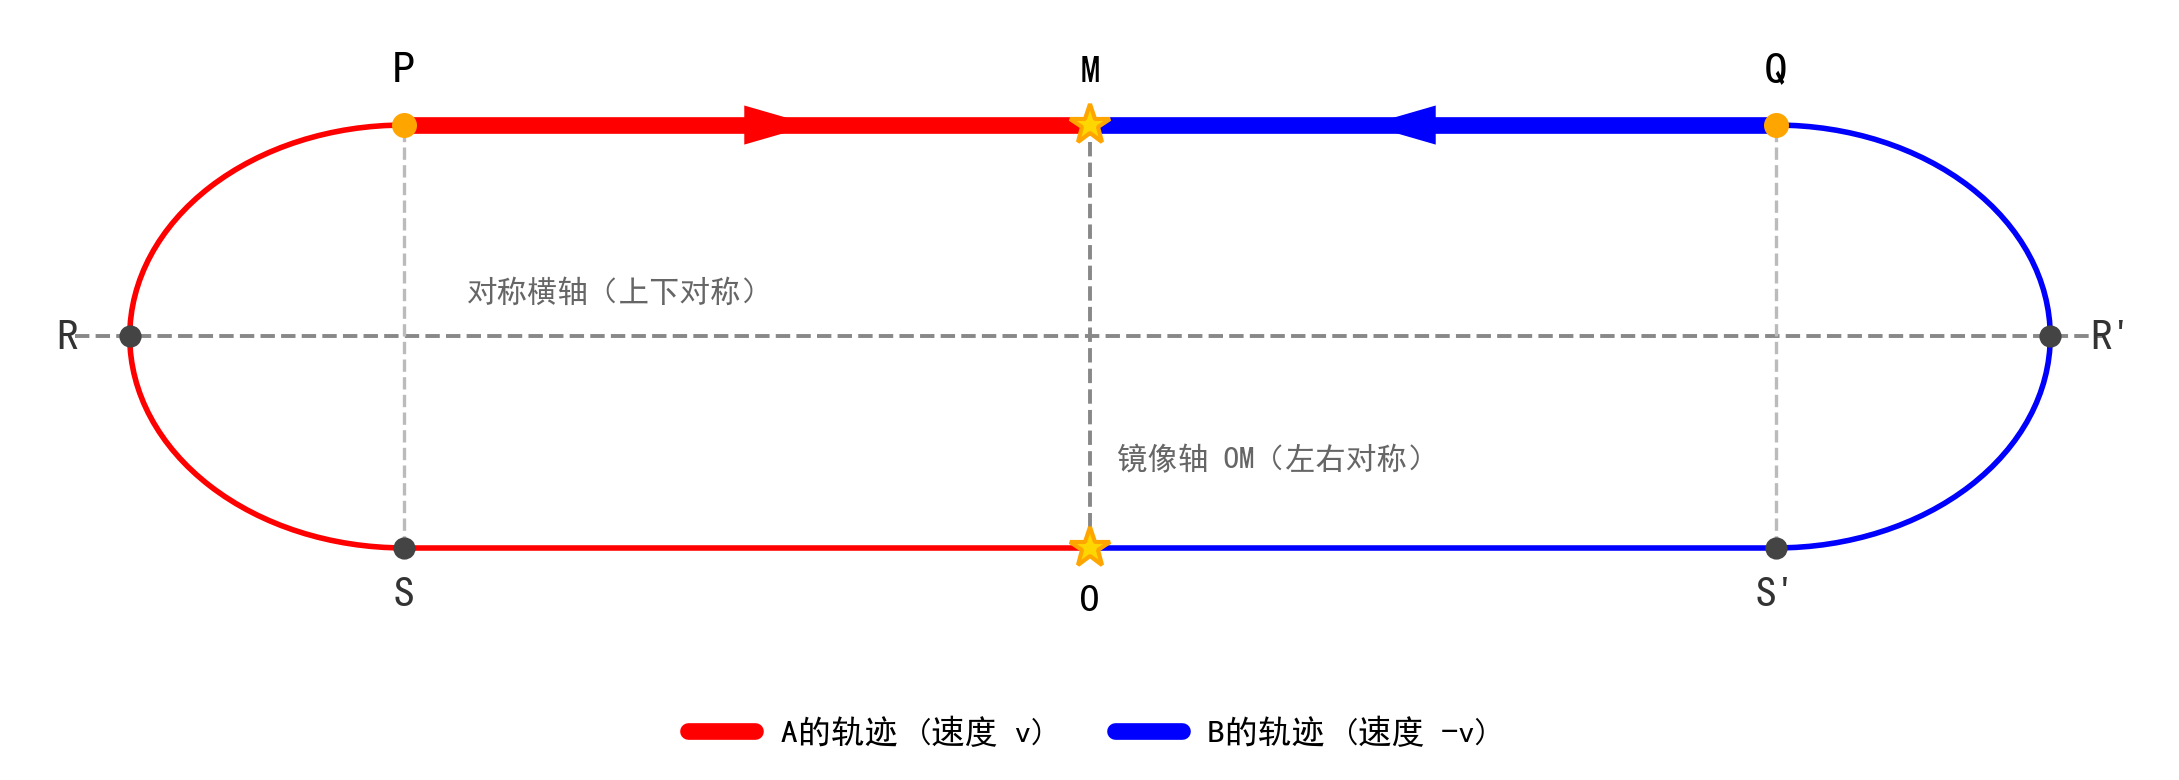
\includegraphics[width=0.95\linewidth,height=\textheight,keepaspectratio]{chapters/images/symmetric.png}

}

\caption{\label{fig-twins}对称双生子实验}

\end{figure}%

\begin{conjecture}[对称性公理]\protect\hypertarget{cnj-symmetry}{}\label{cnj-symmetry}

根据实验设定，路径 \(O \rightarrow P \rightarrow M\) 与
\(O \rightarrow Q \rightarrow M\) 关于中心轴 \(OM\)
完美镜像对称。即：\(A\) 和 \(B\)
的物理经历在空间几何与动力学上完全等价。这一对称性在逻辑上确立了 \(A\)
与 \(B\) 的身份平等与可互换性。

\end{conjecture}

\section{钟慢效应}\label{ux949fux6162ux6548ux5e94}

本章只研究路径分段（定义~\ref{def-path-segments}）中第 2
阶段直线段的惯性运动过程。

在 \(A\) 的静止参考系 \(S_A\) 中，\(B\) 以相对速度 \(v_{B/A}\)
运动。按洛伦兹变换\textsuperscript{{[}\citeproc{ref-einstein1905}{1}{]}}（推导见
章节~\ref{sec-transform-derivation}），\(A\) 测量 \(B\) 的时间会发生膨胀
式~\ref{eq-time-dilation-A}。

\begin{equation}\protect\phantomsection\label{eq-time-dilation-A}{
\Delta t_A = \gamma \left( \Delta t_B + \frac{v_{B/A} \Delta x_B}{c^2} \right)
\quad \Longrightarrow \quad
\Delta t_B = \frac{1}{\gamma} \Delta t_A
}\end{equation}

在 式~\ref{eq-time-dilation-A} 中，\(B\) 在其自身静止系 \(S_B\)
中位置不变，故 \(\Delta x_B = 0\)；\(\Delta t_B\) 是 \(A\) 在 \(S_A\)
系中由洛伦兹变换算出的 \(B\) 的时间，它表明 \(A\) 测得的 \(B\)
的时间流逝更慢。同理，在 \(B\) 的静止系 \(S_B\) 中，\(B\) 也会得出 \(A\)
的时间流逝更慢的结论。

\section{对称性约束}\label{ux5bf9ux79f0ux6027ux7ea6ux675f}

根据 公理~\ref{cnj-symmetry}（对称性公理），\(A\) 和 \(B\)
经历了完全镜像对称的物理过程。在 \(M\)
点相遇时，两者随身时钟的读数相等，即 式~\ref{eq-AQB}。

\begin{equation}\protect\phantomsection\label{eq-AQB}{
\tau_{A} = \tau_{B}
}\end{equation}

\section{实验结论}\label{ux5b9eux9a8cux7ed3ux8bba}

在满足洛伦兹变换的条件的前提下，洛伦兹变换测量得到的``时间不一致''，对称性确定的``随身时钟时相等''。这说明：洛伦兹变换测量出的时间差异，并不等同于物理上时钟实际经历的差异。``钟慢效应''是特定理论下的测量结果，它不等同于随身时钟读数的物理过程的真实发生。

\bookmarksetup{startatroot}

\chapter{伽利略变换与洛伦兹变换的推导}\label{sec-transform-derivation}

\section{公理设定}\label{ux516cux7406ux8bbeux5b9a}

本章的全部结果都从三条前提推出：坐标变换的线性性、一个``不变对象''的存在，以及变换集合的群结构。前两条与群结构为两种变换所共有；真正决定结论的，是``不变对象''取什么------它把推导分成两支，一支给出伽利略变换，一支给出洛伦兹变换。这条不预设光速不变、仅由时空均匀性、各向同性与群结构导出变换的路线，在文献中已有系统论述\textsuperscript{{[}\citeproc{ref-levyleblond1976}{2},\citeproc{ref-berzigorini1969}{3}{]}}。

\textbf{关于本章与第 章节~\ref{sec-invariant-speed-group} 章的分工。}
本章采用``两条第三公理并列、二选一''的叙述：先给出两条候选公理，再分别推出一种变换。第
章节~\ref{sec-invariant-speed-group}
章保留本章的全部算式，改用另一种叙述：把``存在不变对象''换成``存在恒速
\(K\)''，于是两支不再是并列的两个理论，而是同一个以 \(K\)
为参数的群族的两个端点；``不变时间''也随之由独立公理降为 \(K=\infty\)
处的推论。两种叙述的算式完全相同，差别只在解读方式；本章不预设哪一种，第
章节~\ref{sec-invariant-speed-group} 章给出后一种的完整论证。

\textbf{公共公理}

\begin{conjecture}[均匀性假设（线性变换）]\protect\hypertarget{cnj-homogeneity}{}\label{cnj-homogeneity}

空间是均匀的，时间是均匀的。因此，两个惯性系 \(S\) 和 \(S'\)
之间的坐标变换必须是线性变换（齐次线性变换加平移，这里取原点重合的齐次部分）。

\end{conjecture}

\begin{conjecture}[协变性（群结构）]\protect\hypertarget{cnj-covariance}{}\label{cnj-covariance}

所有的空间方向是对称的（各向同性），且变换构成的集合必须形成``群''：即连续做两次变换等于做一次变换，且存在逆变换回到原坐标系。

\end{conjecture}

\textbf{第三条公理：不变对象（二选一）}

\begin{conjecture}[存在不变时间（绝对同时性）]\protect\hypertarget{cnj-invariant-time}{}\label{cnj-invariant-time}

存在一个在所有惯性系中取值相同的时间刻度，即同时性与参考系无关，等时面在变换下不变。形式地：若
\(t = 0\)，则在 \(S'\) 中必有 \(t' = 0\)。

\end{conjecture}

\begin{conjecture}[存在不变速度]\protect\hypertarget{cnj-invariant-speed}{}\label{cnj-invariant-speed}

存在一个恒定的特征速度 \(c\)，在任何参考系中，沿任意方向测量该速度都恒为
\(c\)。形式地：若 \(x = ct\)，则在 \(S'\) 中必有 \(x' = ct'\)；若
\(x = -ct\)，则 \(x' = -ct'\)。

\end{conjecture}

两条第三公理在本章被并列看待，可视为互为对偶：一条把\textbf{时间轴}定为不变量，另一条把\textbf{速度轴}定为不变量。至于二者是``并列的两个前提''还是``同一条陈述的两个取值''，本章不作判断，留给第
章节~\ref{sec-invariant-speed-group} 章。

\begin{longtable}[]{@{}
  >{\raggedright\arraybackslash}p{(\linewidth - 4\tabcolsep) * \real{0.3333}}
  >{\raggedright\arraybackslash}p{(\linewidth - 4\tabcolsep) * \real{0.3333}}
  >{\raggedright\arraybackslash}p{(\linewidth - 4\tabcolsep) * \real{0.3333}}@{}}
\caption{第三条公理的两种取法}\label{tbl-axiom-duality}\tabularnewline
\toprule\noalign{}
\begin{minipage}[b]{\linewidth}\raggedright
\end{minipage} & \begin{minipage}[b]{\linewidth}\raggedright
公理~\ref{cnj-invariant-time}（→ 伽利略）
\end{minipage} & \begin{minipage}[b]{\linewidth}\raggedright
公理~\ref{cnj-invariant-speed}（→ 洛伦兹）
\end{minipage} \\
\midrule\noalign{}
\endfirsthead
\toprule\noalign{}
\begin{minipage}[b]{\linewidth}\raggedright
\end{minipage} & \begin{minipage}[b]{\linewidth}\raggedright
公理~\ref{cnj-invariant-time}（→ 伽利略）
\end{minipage} & \begin{minipage}[b]{\linewidth}\raggedright
公理~\ref{cnj-invariant-speed}（→ 洛伦兹）
\end{minipage} \\
\midrule\noalign{}
\endhead
\bottomrule\noalign{}
\endlastfoot
不变对象 & 等时面 \(t = 0\) & 特征射线 \(x = ct\) \\
形式条件 & \(t = 0 \Rightarrow t' = 0\) &
\(x = ct \Rightarrow x' = ct'\) \\
直观说法 & 不存在有限的不变速度 & 存在有限的不变速度 \(c\) \\
\end{longtable}

\section{建立一般线性变换形式}\label{ux5efaux7acbux4e00ux822cux7ebfux6027ux53d8ux6362ux5f62ux5f0f}

设 \(S'\) 系相对于 \(S\) 系以速度 \(v\) 沿 \(x\)
轴正向运动，两系对应的坐标轴两两平行，且在 \(t = t' = 0\)
时原点重合。两系的几何关系如图 图~\ref{fig-lorentz-frames} 所示。

\begin{figure}

\centering{

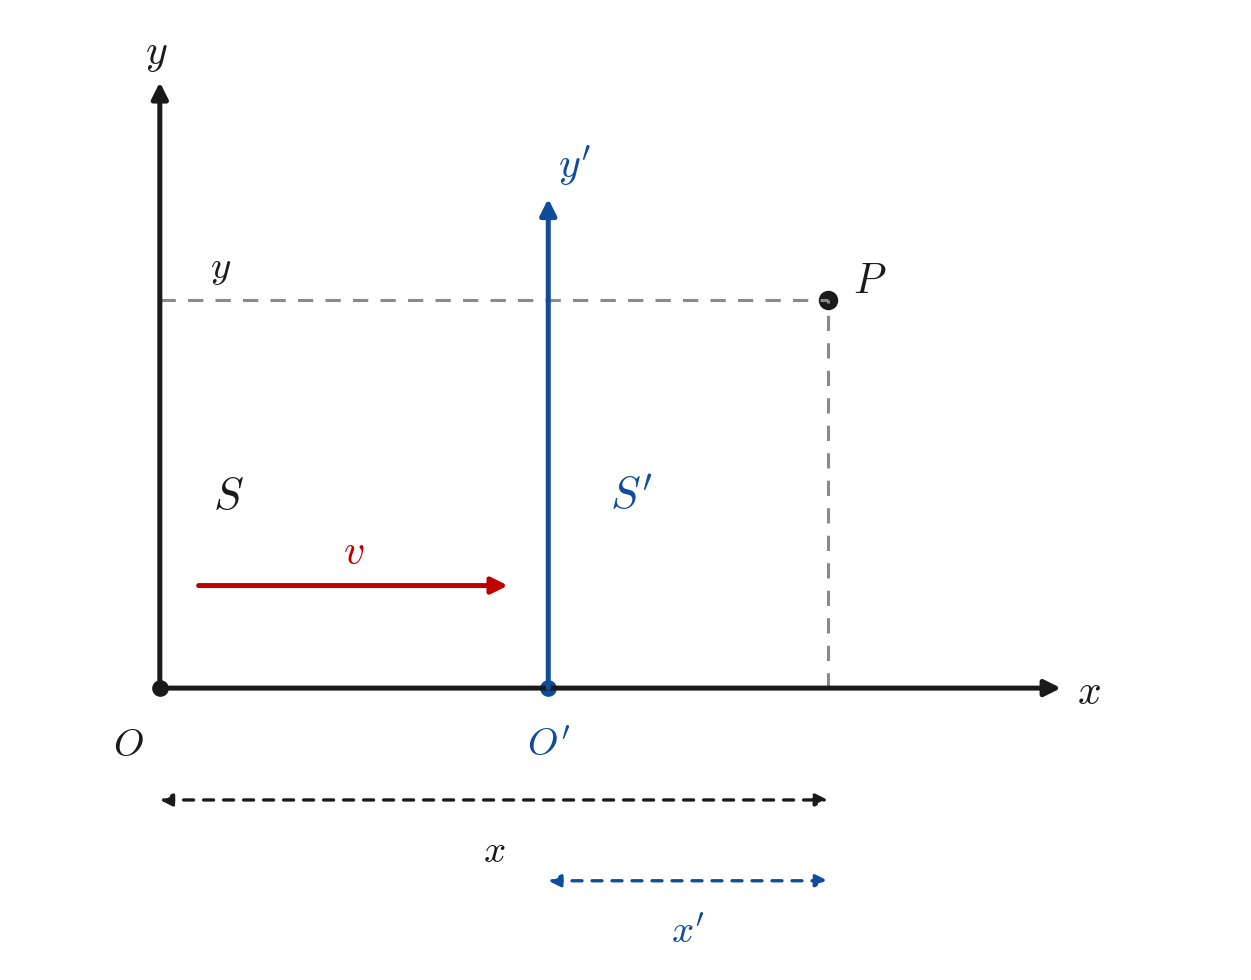
\includegraphics[width=0.6\linewidth,height=\textheight,keepaspectratio]{chapters/images/lorentz-frames.png}

}

\caption{\label{fig-lorentz-frames}两惯性系的坐标变换示意：惯性系 \(S\)
与 \(S'\) 坐标轴对应平行，\(S'\) 系以速度 \(v\) 沿 \(x\) 轴正向相对
\(S\) 系运动，同一事件 \(P\) 在两系中的横坐标分别为 \(x\) 与
\(x'\)，纵坐标 \(y' = y\)}

\end{figure}%

本节的坐标列向量\textbf{统一按 \((t, x)\)
排列}：时间分量在前、空间分量在后，与 小节~\ref{sec-lorentz-4d}
的四维顺序 \((t, x, y, z)\) 完全一致。由
公理~\ref{cnj-homogeneity}，\((t, x)\) 平面内的线性变换必为

\begin{equation}\protect\phantomsection\label{eq-lambda}{
\begin{pmatrix} t' \\ x' \end{pmatrix}
=
\begin{pmatrix} A & B \\ C & D \end{pmatrix}
\begin{pmatrix} t \\ x \end{pmatrix}
}\end{equation}

即

\begin{equation}\protect\phantomsection\label{eq-lin-t}{
t' = A t + B x
}\end{equation}

\begin{equation}\protect\phantomsection\label{eq-lin-x}{
x' = C t + D x
}\end{equation}

其中 \(A, B, C, D\) 是只依赖于 \(v\) 与 \(c\) 的待定常数。

接下来的推导是\textbf{四步消参}：线性性留下四个待定常数，下面四条约束各消去一个。前两条约束只用到``\(S'\)
以速度 \(v\) 相对 \(S\)
运动''这一几何设定，与第三条公理无关，因此两种变换共享；分歧只出现在后两条。

\begin{longtable}[]{@{}llll@{}}
\caption{四步消参：两条公共约束，两条分支约束}\label{tbl-roadmap}\tabularnewline
\toprule\noalign{}
步骤 & 依据 & 伽利略 & 洛伦兹 \\
\midrule\noalign{}
\endfirsthead
\toprule\noalign{}
步骤 & 依据 & 伽利略 & 洛伦兹 \\
\midrule\noalign{}
\endhead
\bottomrule\noalign{}
\endlastfoot
约束 1 & \(S'\) 的原点 & \(C = -Dv\) & \(C = -Dv\) \\
约束 2 & 相对速度 & \(D = A\) & \(D = A\) \\
约束 3 & 不变对象 & \(B = 0\) & \(B = -Av/c^{2}\) \\
约束 4 & 群结构 & \(A = 1\) & \(A = \gamma\) \\
\end{longtable}

\section{公共约束}\label{ux516cux5171ux7ea6ux675f}

\subsection{\texorpdfstring{约束 1：追踪 \(S'\)
的原点}{约束 1：追踪 S\textquotesingle{} 的原点}}\label{ux7ea6ux675f-1ux8ffdux8e2a-s-ux7684ux539fux70b9}

\(S'\) 的原点满足 \(x' = 0\)，它在 \(S\) 系中对应 \(x = vt\)。代入
\(x' = Ct + Dx\)：

\begin{equation}\protect\phantomsection\label{eq-constraint-origin}{
0 = C t + D(vt) = (C + Dv)\,t
\quad \Longrightarrow \quad
C = -Dv
}\end{equation}

于是 式~\ref{eq-lambda} 收缩为

\begin{equation}\protect\phantomsection\label{eq-after-origin}{
\begin{aligned}
t' &= A t + B x \\
x' &= D(x - vt)
\end{aligned}
}\end{equation}

\subsection{约束
2：相对速度}\label{ux7ea6ux675f-2ux76f8ux5bf9ux901fux5ea6}

由相对性原理（公理~\ref{cnj-covariance}），\(S\) 系在自己看来静止，而在
\(S'\) 系中必须以速度 \(-v\) 退行，即其原点 \(x = 0\) 满足
\(x' = -v t'\)。

在 式~\ref{eq-after-origin} 中令 \(x = 0\)，得
\(t' = A t\)、\(x' = -Dv\,t\)，于是 \(x'/t' = -Dv/A\)。要求它等于
\(-v\)（\(v \neq 0\)；\(v = 0\) 时变换退化为恒等，\(A = D = 1\)
自动成立）：

\begin{equation}\protect\phantomsection\label{eq-constraint-velocity}{
-\frac{Dv}{A} = -v
\quad \Longrightarrow \quad
D = A
}\end{equation}

至此两种变换共有一个形式，只剩 \(A\)、\(B\) 两个参数：

\begin{equation}\protect\phantomsection\label{eq-matrix-form}{
\Lambda = \begin{pmatrix} A & B \\ -Av & A \end{pmatrix}
}\end{equation}

分岔点就在 \(B\) 与 \(A\) 上：\(B\) 由第三条公理定，\(A\)
由群结构配合它定。

\section{伽利略变换}\label{ux4f3dux5229ux7565ux53d8ux6362}

\subsection{约束
3G：不变时间}\label{ux7ea6ux675f-3gux4e0dux53d8ux65f6ux95f4}

由 公理~\ref{cnj-invariant-time}，\(t = 0 \Rightarrow t' = 0\)。在
式~\ref{eq-lin-t} 中令 \(t = 0\)，得 \(t' = Bx\)；要求它对一切 \(x\)
为零，故

\begin{equation}\protect\phantomsection\label{eq-constraint-time}{
B = 0
}\end{equation}

于是变换进一步收缩为
\(t' = A t\)、\(x' = A(x - vt)\)------这是一个\textbf{保时}的变换。

\subsection{约束 4G：群结构}\label{ux7ea6ux675f-4gux7fa4ux7ed3ux6784}

由 公理~\ref{cnj-covariance}，变换集合构成群，故速度为 \(v\)
的变换与速度为 \(-v\) 的变换互逆：\(\Lambda(v)\,\Lambda(-v) = I\)。

把 \(v \to -v\) 代入 式~\ref{eq-matrix-form}（此时
\(B = 0\)）；由各向同性，\(A\) 只依赖速率大小而与此方向无关，故
\(A(-v) = A(v) \equiv A\)：

\[
\Lambda(-v) = \begin{pmatrix} A & 0 \\ Av & A \end{pmatrix}
\]

两者相乘，非对角元两两相消，对角元给出 \(A^{2}\)：

\begin{equation}\protect\phantomsection\label{eq-galilean-product}{
\Lambda(v)\,\Lambda(-v)
=
\begin{pmatrix} A & 0 \\ -Av & A \end{pmatrix}
\begin{pmatrix} A & 0 \\ Av & A \end{pmatrix}
=
A^{2} I
}\end{equation}

要求乘积为单位阵，得 \(A^{2} = 1\)。再由 \(v \to 0\)
时变换必须连续地退化为恒等变换（\(A \to 1\)），取正根：

\begin{equation}\protect\phantomsection\label{eq-galilean-a}{
A = 1
}\end{equation}

\subsection{结果}\label{ux7ed3ux679c}

将 \(A = 1\)、\(B = 0\) 代回 式~\ref{eq-lambda}：

\begin{equation}\protect\phantomsection\label{eq-galilean-t}{
t' = t
}\end{equation}

\begin{equation}\protect\phantomsection\label{eq-galilean-x}{
x' = x - vt
}\end{equation}

写成矩阵形式

\begin{equation}\protect\phantomsection\label{eq-galilean-mat}{
\begin{pmatrix} t' \\ x' \end{pmatrix}
=
\begin{pmatrix} 1 & 0 \\ -v & 1 \end{pmatrix}
\begin{pmatrix} t \\ x \end{pmatrix}
}\end{equation}

这就是伽利略变换：时间绝对（\(t' = t\)），空间坐标按 \(x' = x - vt\)
随参考系平移。

\textbf{一致性检验。}
两次同向伽利略变换应当等于一次合成变换，\(\Lambda(v_{1})\,\Lambda(v_{2}) = \Lambda(v_{1} + v_{2})\)。直接相乘：

\[
\begin{pmatrix} 1 & 0 \\ -v_{1} & 1 \end{pmatrix}
\begin{pmatrix} 1 & 0 \\ -v_{2} & 1 \end{pmatrix}
=
\begin{pmatrix} 1 & 0 \\ -(v_{1} + v_{2}) & 1 \end{pmatrix}
\]

速度按算术相加，群结构闭合。

\section{洛伦兹变换}\label{ux6d1bux4f26ux5179ux53d8ux6362}

爱因斯坦以``光速不变原理''为前提\textsuperscript{{[}\citeproc{ref-einstein1905}{1}{]}}；本节的推导不引入任何具体物理对象，只用
公理~\ref{cnj-invariant-speed} 这一条关于变换形式的约束。

\subsection{约束
3L：不变速度}\label{ux7ea6ux675f-3lux4e0dux53d8ux901fux5ea6}

由 公理~\ref{cnj-invariant-speed}，要求
\(x = ct \Rightarrow x' = ct'\)。取满足 \(x = ct\) 的事件；由
式~\ref{eq-constraint-velocity} 有 \(D = A\)，故
式~\ref{eq-after-origin} 给出 \(x' = A(x - vt)\)。用它和
式~\ref{eq-lin-t} 构造组合 \(x' - ct'\)：

\[
x' - c t'
= A(ct - vt) - c\,(At + Bct)
= -\left(Av + Bc^{2}\right)t
\]

要求该组合恒为零，即得

\begin{equation}\protect\phantomsection\label{eq-constraint-light}{
Av + Bc^{2} = 0
\quad \Longrightarrow \quad
B = -\frac{Av}{c^{2}}
}\end{equation}

对满足 \(x = -ct\) 的事件，同样构造 \(x' + ct'\)，得到的是同一个约束
\(Av + Bc^{2} = 0\)，不产生新的限制。

\subsection{约束 4L：群结构}\label{ux7ea6ux675f-4lux7fa4ux7ed3ux6784}

与伽利略一支同样的理由（公理~\ref{cnj-covariance}）：\(\Lambda(v)\,\Lambda(-v) = I\)。由各向同性，\(A(-v) = A(v) \equiv A\)，故

\[
\Lambda(v) = \begin{pmatrix} A & -Av/c^{2} \\ -Av & A \end{pmatrix},
\qquad
\Lambda(-v) = \begin{pmatrix} A & Av/c^{2} \\ Av & A \end{pmatrix}
\]

两者相乘，非对角元两两相消，对角元给出
\(A^{2}\left(1 - v^{2}/c^{2}\right)\)：

\begin{equation}\protect\phantomsection\label{eq-boost-product}{
\begin{aligned}
\Lambda(v) \Lambda(-v) &= \begin{pmatrix} A & -Av/c^2 \\ -Av & A \end{pmatrix} \begin{pmatrix} A & Av/c^2 \\ Av & A \end{pmatrix} \\
&= \begin{pmatrix} A^2 \left(1 - \frac{v^2}{c^2}\right) & 0 \\ 0 & A^2 \left(1 - \frac{v^2}{c^2}\right) \end{pmatrix} \\
&= A^2 \left(1 - \frac{v^2}{c^2}\right) I
\end{aligned}
}\end{equation}

要求乘积为单位阵，得

\begin{equation}\protect\phantomsection\label{eq-gamma-def}{
A^{2}\left(1 - \frac{v^{2}}{c^{2}}\right) = 1
\quad \Longrightarrow \quad
A = \frac{1}{\sqrt{1 - v^{2}/c^{2}}} \equiv \gamma
}\end{equation}

根号取正号：\(v \to 0\) 时变换必须连续地退化为恒等变换，\(A \to 1\)。

\subsection{结果}\label{ux7ed3ux679c-1}

\begin{equation}\protect\phantomsection\label{eq-final-t}{
t' = \gamma\left( t - \frac{v}{c^{2}}x \right)
}\end{equation}

\begin{equation}\protect\phantomsection\label{eq-final-x}{
x' = \gamma(x - vt)
}\end{equation}

写成矩阵形式 式~\ref{eq-final-matrix}：

\begin{equation}\protect\phantomsection\label{eq-final-matrix}{
\begin{pmatrix} t' \\ x' \end{pmatrix}
=
\begin{pmatrix} \gamma & -\gamma v/c^{2} \\ -\gamma v & \gamma \end{pmatrix}
\begin{pmatrix} t \\ x \end{pmatrix}
}\end{equation}

\textbf{一致性检验。}
两次同向洛伦兹变换同样应当等于一次合成变换。直接相乘得

\[
\begin{aligned}
\Lambda(v_1)\Lambda(v_2) &= \begin{pmatrix} \gamma_1 & -\gamma_1 v_1/c^2 \\ -\gamma_1 v_1 & \gamma_1 \end{pmatrix} \begin{pmatrix} \gamma_2 & -\gamma_2 v_2/c^2 \\ -\gamma_2 v_2 & \gamma_2 \end{pmatrix} \\
&= \begin{pmatrix} \gamma_1\gamma_2 \left(1 + \frac{v_1v_2}{c^2}\right) & -\frac{\gamma_1\gamma_2}{c^2}(v_1 + v_2) \\ -\gamma_1\gamma_2(v_1 + v_2) & \gamma_1\gamma_2 \left(1 + \frac{v_1v_2}{c^2}\right) \end{pmatrix} \\
&= \gamma_1\gamma_2 \left(1 + \frac{v_1v_2}{c^2}\right) \begin{pmatrix} 1 & -\frac{v_1+v_2}{c^2(1 + v_1v_2/c^2)} \\ -\frac{v_1+v_2}{1 + v_1v_2/c^2} & 1 \end{pmatrix}
\end{aligned}
\]

根据速度合成定理，令 \(V\) 为：

\[
V = \frac{v_1 + v_2}{1 + v_1v_2/c^2}
\]

最终将 \(V\) 代入上式，得到结果：

\[
\Lambda(v_1)\Lambda(v_2) = \gamma_1\gamma_2 \left(1 + \frac{v_1v_2}{c^2}\right) \begin{pmatrix} 1 & -V/c^2 \\ -V & 1 \end{pmatrix}
\]

而
\(\gamma_{1}\gamma_{2}\left(1 + v_{1}v_{2}/c^{2}\right) = \gamma(V)\)：

\[
\begin{aligned}
\gamma(V) &= \frac{1}{\sqrt{1 - V^2/c^2}} \\
&= \frac{1}{\sqrt{1 - \frac{1}{c^2} \left( \frac{v_1 + v_2}{1 + v_1v_2/c^2} \right)^2}} \\
&= \frac{1}{\sqrt{\frac{c^2(1 + v_1v_2/c^2)^2 - (v_1 + v_2)^2}{c^2(1 + v_1v_2/c^2)^2}}}
\end{aligned}
\]

将分子部分展开，进行代数化简：

\[
\begin{aligned}
&c^2(1 + v_1v_2/c^2)^2 - (v_1 + v_2)^2 \\
&= c^2 \left( 1 + 2\frac{v_1v_2}{c^2} + \frac{v_1^2v_2^2}{c^4} \right) - (v_1^2 + 2v_1v_2 + v_2^2) \\
&= \left( c^2 + 2v_1v_2 + \frac{v_1^2v_2^2}{c^2} \right) - v_1^2 - 2v_1v_2 - v_2^2 \\
&= c^2 - v_1^2 - v_2^2 + \frac{v_1^2v_2^2}{c^2} \\
&= c^2 \left( 1 - \frac{v_1^2}{c^2} - \frac{v_2^2}{c^2} + \frac{v_1^2v_2^2}{c^4} \right) \\
&= c^2 \left( 1 - \frac{v_1^2}{c^2} \right) \left( 1 - \frac{v_2^2}{c^2} \right)
\end{aligned}
\]

\[
\begin{aligned}
\gamma(V) &= \frac{1}{\sqrt{\frac{c^2 \left( 1 - \frac{v_1^2}{c^2} \right) \left( 1 - \frac{v_2^2}{c^2} \right)}{c^2(1 + v_1v_2/c^2)^2}}} \\
&= \frac{1 + v_1v_2/c^2}{\sqrt{1 - v_1^2/c^2} \cdot \sqrt{1 - v_2^2/c^2}} \\
&= \gamma_1 \gamma_2 \left( 1 + \frac{v_1v_2}{c^2} \right)
\end{aligned}
\]

故乘积恰为
\(\Lambda(V)\)：速度按相对论加法合成，群结构同样闭合，只是合成律不再是算术相加。

\section{两种变换的关系}\label{ux4e24ux79cdux53d8ux6362ux7684ux5173ux7cfb}

\textbf{1. 逐项对照}

\begin{longtable}[]{@{}
  >{\raggedright\arraybackslash}p{(\linewidth - 4\tabcolsep) * \real{0.3333}}
  >{\raggedright\arraybackslash}p{(\linewidth - 4\tabcolsep) * \real{0.3333}}
  >{\raggedright\arraybackslash}p{(\linewidth - 4\tabcolsep) * \real{0.3333}}@{}}
\caption{两种变换的逐项对照}\label{tbl-comparison}\tabularnewline
\toprule\noalign{}
\begin{minipage}[b]{\linewidth}\raggedright
\end{minipage} & \begin{minipage}[b]{\linewidth}\raggedright
伽利略（式~\ref{eq-galilean-t}、式~\ref{eq-galilean-x}）
\end{minipage} & \begin{minipage}[b]{\linewidth}\raggedright
洛伦兹（式~\ref{eq-final-t}、式~\ref{eq-final-x}）
\end{minipage} \\
\midrule\noalign{}
\endfirsthead
\toprule\noalign{}
\begin{minipage}[b]{\linewidth}\raggedright
\end{minipage} & \begin{minipage}[b]{\linewidth}\raggedright
伽利略（式~\ref{eq-galilean-t}、式~\ref{eq-galilean-x}）
\end{minipage} & \begin{minipage}[b]{\linewidth}\raggedright
洛伦兹（式~\ref{eq-final-t}、式~\ref{eq-final-x}）
\end{minipage} \\
\midrule\noalign{}
\endhead
\bottomrule\noalign{}
\endlastfoot
时间 & \(t' = t\) & \(t' = \gamma\left(t - vx/c^{2}\right)\) \\
空间 & \(x' = x - vt\) & \(x' = \gamma(x - vt)\) \\
矩阵 & \(\begin{pmatrix} 1 & 0 \\ -v & 1 \end{pmatrix}\) &
\(\begin{pmatrix} \gamma & -\gamma v/c^{2} \\ -\gamma v & \gamma \end{pmatrix}\) \\
不变量 & \(\Delta t\)（绝对时间） &
\(c^{2}\Delta t^{2} - \Delta x^{2}\)（时空间隔） \\
速度合成 & 算术相加 \(v_{1} + v_{2}\) & 相对论加法 \\
\end{longtable}

\textbf{2. \(c \to \infty\) 的极限}

把洛伦兹变换中的 \(c\)
取无穷：\(\gamma \to 1\)，\(\gamma v/c^{2} \to 0\)，式~\ref{eq-final-t}
与 式~\ref{eq-final-x} 逐项退化为 式~\ref{eq-galilean-t} 与
式~\ref{eq-galilean-x}。也就是说，

\begin{quote}
\textbf{伽利略变换是洛伦兹变换在 \(c \to \infty\) 下的极限。}
\end{quote}

这与两条第三公理的对偶性一致：\(c\) 取有限值对应``存在不变速度''，\(c\)
取无穷则意味着不存在有限的不变速度------那正是
公理~\ref{cnj-invariant-time}
所陈述的内容。所以两条公理并非两个互不相干的前提，而是同一条陈述在有限与无限两处的取值。

\textbf{3. 群结构}

两支各自闭合（合成律见各自的一致性检验）。在群论上，伽利略群是洛伦兹群在
\(c \to \infty\) 下的 Inönü--Wigner
收缩；单就群本身而言，洛伦兹群是``更大''的那一个，伽利略群是它在收缩极限下的退化结果。

\section{推广到四维时空}\label{sec-lorentz-4d}

前面的推导在 \((t, x)\)
平面内完成，对两种变换同样适用。本节补齐四维图景：先由对称性证明横向坐标
\(y\)、\(z\) 在变换下不变，再分别给出四维形式的伽利略变换与洛伦兹变换。

\subsection{横向坐标不变：对称性论证}\label{ux6a2aux5411ux5750ux6807ux4e0dux53d8ux5bf9ux79f0ux6027ux8bbaux8bc1}

设两系坐标轴对应平行。\(y\)、\(z\) 坐标的一般线性变换可写为
式~\ref{eq-yz-general}（系数只依赖于 \(v\) 与 \(c\)）：

\begin{equation}\protect\phantomsection\label{eq-yz-general}{
\begin{aligned}
y' &= p\,y + q\,z + \alpha x + \eta t \\
z' &= r\,y + s\,z + \mu x + \nu t
\end{aligned}
}\end{equation}

\textbf{第一步（\(x\) 轴映到 \(x'\) 轴）。} 由各向同性，\(x\)
轴在变换下必须映到 \(x'\) 轴：位于 \(x\) 轴上的点（\(y = z = 0\)）在
\(S'\) 系中的横向坐标必须为零。于是对任意 \(x\)、\(t\) 有
\(\alpha x + \eta t = 0\) 与 \(\mu x + \nu t = 0\)，故

\[
\alpha = \eta = \mu = \nu = 0
\]

\textbf{第二步（反射对称性）。} 将两系的 \(y\)
轴同时反向（\(y \to -y\)，\(y' \to -y'\)），物理情境不变，变换形式应保持不变。在反射后的坐标下
\(-y' = -py + qz\)，即 \(y' = py - qz\)，与原式 \(y' = py + qz\) 比较得
\(q = 0\)；同理，由 \(z \to -z\) 的反射对称性得 \(r = 0\)。于是

\[
y' = p\,y, \qquad z' = s\,z
\]

\textbf{第三步（确定横向比例因子）。} 由 \(y\)、\(z\)
两个横向方向的等价性，\(p = s\)，记为 \(a(v)\)。

\begin{itemize}
\tightlist
\item
  一方面，对上式求逆（即把 \(v\) 换成 \(-v\) 的变换）得
  \(y = a(-v)\,y'\)，故
\end{itemize}

\[
a(v)\,a(-v) = 1
\]

\begin{itemize}
\tightlist
\item
  另一方面，考虑两个由相对性原理（公理~\ref{cnj-covariance}）联系起来的实验：\(S'\)
  系测量静止于 \(S\) 系的横向标尺，由于 \(y'\) 只依赖于
  \(y\)（与同时性无关），测得长度为原来的 \(a(v)\) 倍；\(S\)
  系测量静止于 \(S'\) 系的同一根标尺，测得长度为原来的 \(a(-v)\)
  倍。两个实验的物理地位完全对等（交换两系即可互换），比例因子必须相同，故
  \(a(v) = a(-v)\)。
\end{itemize}

于是 \(a(v)^{2} = 1\)；再由 \(v \to 0\)
时变换连续地退化为恒等变换（\(a \to 1\)），得

\begin{equation}\protect\phantomsection\label{eq-yz-invariant}{
y' = y, \qquad z' = z
}\end{equation}

即\textbf{横向坐标在变换下不变}------这一论证既不涉及 \(B\) 也不涉及
\(A\)，因此对伽利略与洛伦兹两种变换同时成立。于是四维变换在 \((t, x)\)
与 \((y, z)\) 子空间上是分块对角的，前几节在 \((t, x)\)
平面内的推导对四维变换完全充分。

\subsection{四维伽利略变换}\label{ux56dbux7ef4ux4f3dux5229ux7565ux53d8ux6362}

综合 式~\ref{eq-galilean-t}、式~\ref{eq-galilean-x} 与
式~\ref{eq-yz-invariant}，得到四维伽利略变换（变量按 \((t, x, y, z)\)
的顺序排列）：

\begin{equation}\protect\phantomsection\label{eq-galilean-4d}{
\left\{\begin{aligned}
& t' = t \\
& x' = x - vt \\
& y' = y \\
& z' = z
\end{aligned} \right.
}\end{equation}

其矩阵形式为

\begin{equation}\protect\phantomsection\label{eq-galilean-4d-mat}{
\begin{pmatrix}
t' \\ x' \\ y' \\ z'
\end{pmatrix}
=
\begin{pmatrix}
1 & 0 & 0 & 0 \\
-v & 1 & 0 & 0 \\
0 & 0 & 1 & 0 \\
0 & 0 & 0 & 1
\end{pmatrix}
\begin{pmatrix}
t \\ x \\ y \\ z
\end{pmatrix}
}\end{equation}

\subsection{四维洛伦兹变换}\label{ux56dbux7ef4ux6d1bux4f26ux5179ux53d8ux6362}

综合 式~\ref{eq-final-t}、式~\ref{eq-final-x} 与
式~\ref{eq-yz-invariant}，得到四维洛伦兹变换：

\begin{equation}\protect\phantomsection\label{eq-lorentz-4d}{
\left\{\begin{aligned}
& t' = \gamma\left(t - \frac{v}{c^{2}}x \right) \\
& x' = \gamma(x - vt) \\
& y' = y \\
& z' = z
\end{aligned} \right.
}\end{equation}

其矩阵形式为 式~\ref{eq-lorentz-4d-mat}。

\begin{equation}\protect\phantomsection\label{eq-lorentz-4d-mat}{
\begin{pmatrix}
t' \\ x' \\ y' \\ z'
\end{pmatrix}
=
\begin{pmatrix}
\gamma & -\gamma v/c^{2} & 0 & 0 \\
-\gamma v & \gamma & 0 & 0 \\
0 & 0 & 1 & 0 \\
0 & 0 & 0 & 1
\end{pmatrix}
\begin{pmatrix}
t \\ x \\ y \\ z
\end{pmatrix}
}\end{equation}

取 \(x^{0} = ct\) 并记
\(\beta = v/c\)，四个分量具有相同的长度量纲，式~\ref{eq-final-matrix} 的
\(2 \times 2\) 块化为对称形式 式~\ref{eq-lorentz-4d-beta}。

\begin{equation}\protect\phantomsection\label{eq-lorentz-4d-beta}{
\begin{pmatrix}
ct' \\ x' \\ y' \\ z'
\end{pmatrix}
=
\begin{pmatrix}
\gamma & -\gamma\beta & 0 & 0 \\
-\gamma\beta & \gamma & 0 & 0 \\
0 & 0 & 1 & 0 \\
0 & 0 & 0 & 1
\end{pmatrix}
\begin{pmatrix}
ct \\ x \\ y \\ z
\end{pmatrix}
}\end{equation}

\subsection{时空间隔不变性}\label{ux65f6ux7a7aux95f4ux9694ux4e0dux53d8ux6027}

定义两事件之间的时空间隔（以下取原点重合的事件，即
\(\Delta t = t\)、\(\Delta x = x\) 等）

\begin{equation}\protect\phantomsection\label{eq-interval}{
s^{2} = c^{2}\Delta t^{2} - \Delta x^{2} - \Delta y^{2} - \Delta z^{2}
}\end{equation}

由 式~\ref{eq-lorentz-4d-beta} 读出
\(ct' = \gamma(ct - \beta x)\)、\(x' = \gamma(x - \beta ct)\)，以及
\(y' = y\)、\(z' = z\)。直接计算

\begin{equation}\protect\phantomsection\label{eq-interval-verify}{
\begin{aligned}
c^{2}t'^{2} - x'^{2}
&= \gamma^{2}\left[(ct - \beta x)^{2} - (x - \beta ct)^{2}\right] \\
&= \gamma^{2}(c^{2}t^{2} + \beta^{2}x^{2} - x^{2} - \beta^{2}c^{2}t^{2}) \\
&= \gamma^{2}\left((1 - \beta^{2})c^{2}t^{2} - (1 - \beta^{2}) x^{2}\right)\\
&= \gamma^{2}\left(1 - \beta^{2}\right)\left(c^{2}t^{2} - x^{2}\right) \\
&= c^{2}t^{2} - x^{2}
\end{aligned}
}\end{equation}

末步用了
\(\gamma^{2}\left(1 - \beta^{2}\right) = 1\)（式~\ref{eq-gamma-def}）。横向分量不参与运算（\(y' = y\)、\(z' = z\)），故
式~\ref{eq-interval} 整体不变：

\begin{equation}\protect\phantomsection\label{eq-interval-invariance}{
c^{2}t'^{2} - x'^{2} - y'^{2} - z'^{2}
=
c^{2}t^{2} - x^{2} - y^{2} - z^{2}
}\end{equation}

\section{讨论}\label{ux8ba8ux8bba}

本章的两种变换出自\textbf{同一套推导}。线性性给出 \(A, B, C, D\)
四个待定常数；\(S'\)
的原点与相对速度各消去一个（公共约束）；第三条公理消去 \(B\)；群结构定下
\(A\)。两支的差别全部集中在第三条公理：

\begin{itemize}
\tightlist
\item
  取``存在不变时间''：\(B = 0\)、\(A = 1\)，得\textbf{伽利略变换}；
\item
  取``存在不变速度
  \(c\)''：\(B = -Av/c^{2}\)、\(A = \gamma\)，得\textbf{洛伦兹变换}。
\end{itemize}

整个推导只使用了三条公理------线性性、不变对象的存在与群结构------而未借助电磁学或光的任何具体性质；``不变速度''在此只是一条关于变换形式的约束，与任何具体物理对象无关。

\newpage

\bookmarksetup{startatroot}

\chapter{恒速群}\label{sec-invariant-speed-group}

\section{本章的范围}\label{sec-isg-scope}

第 章节~\ref{sec-transform-derivation}
章从三条弱前提出发，同时导出了伽利略变换与洛伦兹变换。本章保留那套推导的全部算式，但更换其\textbf{解读方式}：把两条变换不看作两个并列的理论，而看作\textbf{同一个参数化群族的两个端点}。

\section{两种解读方式}\label{sec-isg-two-views}

\subsection{原解读}\label{ux539fux89e3ux8bfb}

存在不变对象。取「存在不变时间」得伽利略变换；取「存在不变速度
\(c\)」得洛伦兹变换。

\subsection{新解读}\label{ux65b0ux89e3ux8bfb}

存在恒速 \(K\)（\(K\) 为待定参数）。由此得一个参数化的群族。取 \(K\)
有限，得洛伦兹型变换；取 \(K=\infty\)，得伽利略变换。

\subsection{差在哪里}\label{ux5deeux5728ux54eaux91cc}

两种解读的算式\textbf{完全相同}，差别只在于：\textbf{「不变时间」是一条独立公设，还是
\(K=\infty\) 的推论单参数族}

新解读取消了这一冲突：\textbf{唯一公设是「存在恒速 \(K\)」，\(K\)
是参数；\(K=\infty\) 时，不变时间作为极限性质自动出现。}

这是本章要落笔的第一条：

\begin{proposition}[单参数族]\protect\hypertarget{prp-isg-one-param}{}\label{prp-isg-one-param}

在下述公设 (A1)---(A4) 下，变换构成以 \(K\in(0,\infty]\) 为参数的群族
\(G_K\)；\(t'=t\)（不变时间）是 \(K=\infty\) 情形的推论。

\end{proposition}

\section{公设}\label{sec-isg-axioms}

\textbf{(A1) 线性性。} 两个惯性系之间的坐标变换是线性的。

\textbf{(A2) 空间各向同性。} 空间旋转不改变变换的形式；特别地，沿 \(+x\)
方向速度为 \(v\) 的变换与沿 \(-x\) 方向速度为 \(v\)
的变换之间由空间反射联系。

\textbf{(A3) 群结构。} 变换的集合对复合封闭，含恒等元，每个元素可逆。

\textbf{(A4) 存在恒速 \(K\)。} 存在常数 \(K>0\)，使得：若某物在 \(S\)
系中沿 \(x\) 方向速度为 \(K\)，则其在 \(S'\) 系中沿 \(x'\) 方向速度亦为
\(K\)。

\textbf{说明}：本章不预设 \(K\) 的具体数值。\(K\) 是一个待定参数，公设
(A4) 只断言其存在。

\section{推导}\label{sec-isg-derivation}

限于 1+1 维（\(t,x\)）。由 (A1)，变换写成矩阵形式

\begin{equation}\protect\phantomsection\label{eq-isg-mat}{
\begin{pmatrix} t'\\ x' \end{pmatrix}
=
\begin{pmatrix} A & B\\ C & D \end{pmatrix}
\begin{pmatrix} t\\ x \end{pmatrix}
}\end{equation}

其中 \(A,B,C,D\) 为相对速度 \(v\) 的函数。以下逐步定出它们。

\subsection{\texorpdfstring{第一步：\(S'\) 原点在 \(S\)
中的轨迹}{第一步：S\textquotesingle{} 原点在 S 中的轨迹}}\label{ux7b2cux4e00ux6b65s-ux539fux70b9ux5728-s-ux4e2dux7684ux8f68ux8ff9}

\(S'\) 的原点满足 \(x'=0\)。设其在 \(S\) 系中速度为 \(v\)，即
\(x=vt\)。由 式~\ref{eq-isg-mat} 第二行：

\begin{equation}\protect\phantomsection\label{eq-isg-C}{
C\,t+D\,(vt)=0\quad\Longrightarrow\quad C=-vD
}\end{equation}

\subsection{\texorpdfstring{第二步：\(S\) 原点在 \(S'\)
中的轨迹}{第二步：S 原点在 S\textquotesingle{} 中的轨迹}}\label{ux7b2cux4e8cux6b65s-ux539fux70b9ux5728-s-ux4e2dux7684ux8f68ux8ff9}

\(S\) 的原点满足 \(x=0\)。由 (A2)（空间反射对称），其在 \(S'\)
系中速度为 \(-v\)：

\begin{equation}\protect\phantomsection\label{eq-isg-S-origin}{
x'=-v\,t'
}\end{equation}

把 \(x=0\) 代入 式~\ref{eq-isg-mat}：

\[
t'=A\,t,\qquad x'=C\,t
\]

代入 式~\ref{eq-isg-S-origin}：

\begin{equation}\protect\phantomsection\label{eq-isg-C2}{
C\,t=-v\,(A\,t)\quad\Longrightarrow\quad C=-vA
}\end{equation}

\subsection{\texorpdfstring{第三步：由第一步与第二步得
\(A=D\)}{第三步：由第一步与第二步得 A=D}}\label{ux7b2cux4e09ux6b65ux7531ux7b2cux4e00ux6b65ux4e0eux7b2cux4e8cux6b65ux5f97-ad}

比较 式~\ref{eq-isg-C} 与 式~\ref{eq-isg-C2}（\(v\neq0\) 时）：

\begin{equation}\protect\phantomsection\label{eq-isg-AD}{
-vD=-vA\quad\Longrightarrow\quad D=A
}\end{equation}

代回 式~\ref{eq-isg-C}：

\begin{equation}\protect\phantomsection\label{eq-isg-C3}{
C=-vA
}\end{equation}

至此，式~\ref{eq-isg-mat} 化为

\begin{equation}\protect\phantomsection\label{eq-isg-form}{
t'=A\,(t+\beta x),\qquad x'=A\,(x-vt)
}\end{equation}

其中记 \(B=:A\beta\)，\(\beta\) 为待定函数。

\subsection{\texorpdfstring{第四步：由恒速的存在定
\(\beta\)}{第四步：由恒速的存在定 \textbackslash beta}}\label{ux7b2cux56dbux6b65ux7531ux6052ux901fux7684ux5b58ux5728ux5b9a-beta}

设某物在 \(S\) 系中速度为 \(K\)：\(x=Kt\)。由 式~\ref{eq-isg-form}：

\[
t'=A\,(t+\beta K t)=A\,t\,(1+\beta K)
\]

\[
x'=A\,(Kt-vt)=A\,t\,(K-v)
\]

由 (A4)，其在 \(S'\) 系中速度亦为 \(K\)：

\[
\frac{x'}{t'}=K
\quad\Longrightarrow\quad
\frac{A\,t\,(K-v)}{A\,t\,(1+\beta K)}=K
\]

消去 \(A\,t\)（\(A\neq0,\ t\neq0\)）：

\[
K-v=K\,(1+\beta K)=K+\beta K^{2}
\]

\begin{equation}\protect\phantomsection\label{eq-isg-beta}{
-v=\beta K^{2}
\quad\Longrightarrow\quad
\beta=-\frac{v}{K^{2}}
}\end{equation}

代回 式~\ref{eq-isg-form}，得变换的\textbf{形式}

\begin{equation}\protect\phantomsection\label{eq-isg-family}{
t'=A(v)\Bigl(t-\frac{v\,x}{K^{2}}\Bigr),\qquad
x'=A(v)\,(x-vt)
}\end{equation}

其中 \(A(v)\) 尚未定出，由 (A3)（群结构）确定。

\subsection{\texorpdfstring{第五步：由群结构定
\(A(v)\)}{第五步：由群结构定 A(v)}}\label{ux7b2cux4e94ux6b65ux7531ux7fa4ux7ed3ux6784ux5b9a-av}

把 式~\ref{eq-isg-family} 写成矩阵：

\begin{equation}\protect\phantomsection\label{eq-isg-Lambda}{
\Lambda(v)=A(v)
\begin{pmatrix}
1 & -\dfrac{v}{K^{2}}\\[6pt]
-v & 1
\end{pmatrix}
}\end{equation}

\textbf{复合两个变换。} 先算矩阵部分（记
\(M(v):=\begin{pmatrix}1&-v/K^{2}\\-v&1\end{pmatrix}\)）：

\[
M(v)\,M(u)=
\begin{pmatrix}
1 & -\dfrac{v}{K^{2}}\\[4pt]
-v & 1
\end{pmatrix}
\begin{pmatrix}
1 & -\dfrac{u}{K^{2}}\\[4pt]
-u & 1
\end{pmatrix}
\]

逐项相乘：

\[
=\begin{pmatrix}
1\cdot1+\Bigl(-\dfrac{v}{K^{2}}\Bigr)(-u) &
1\cdot\Bigl(-\dfrac{u}{K^{2}}\Bigr)+\Bigl(-\dfrac{v}{K^{2}}\Bigr)\cdot1\\[10pt]
(-v)\cdot1+1\cdot(-u) &
(-v)\Bigl(-\dfrac{u}{K^{2}}\Bigr)+1\cdot1
\end{pmatrix}
\]

\[
=\begin{pmatrix}
1+\dfrac{uv}{K^{2}} &
-\dfrac{u+v}{K^{2}}\\[10pt]
-(u+v) &
1+\dfrac{uv}{K^{2}}
\end{pmatrix}
=\Bigl(1+\frac{uv}{K^{2}}\Bigr)
\begin{pmatrix}
1 & -\dfrac{w}{K^{2}}\\[6pt]
-w & 1
\end{pmatrix}
\]

其中

\begin{equation}\protect\phantomsection\label{eq-isg-w}{
w:=\frac{u+v}{1+\dfrac{uv}{K^{2}}}
}\end{equation}

即 \(M(v)M(u)=\Bigl(1+\frac{uv}{K^{2}}\Bigr)M(w)\)。

由 (A3)，\(\Lambda(v)\Lambda(u)\) 必须仍属于此族，即

\[
\Lambda(v)\Lambda(u)=\Lambda(w)
\]

\[
A(v)A(u)\Bigl(1+\frac{uv}{K^{2}}\Bigr)M(w)=A(w)M(w)
\]

比较系数：

\begin{equation}\protect\phantomsection\label{eq-isg-func}{
A(v)\,A(u)\Bigl(1+\frac{uv}{K^{2}}\Bigr)=A(w)
}\end{equation}

取 \(u=-v\)，则 \(w=0\)，且 \(A(0)=1\)（恒等变换），代入
式~\ref{eq-isg-func}：

\begin{equation}\protect\phantomsection\label{eq-isg-func2}{
A(v)\,A(-v)\Bigl(1-\frac{v^{2}}{K^{2}}\Bigr)=1
}\end{equation}

由 (A2)（空间反射），\(A(-v)=A(v)\)，故

\begin{equation}\protect\phantomsection\label{eq-isg-A}{
A(v)^{2}=\frac{1}{1-\dfrac{v^{2}}{K^{2}}}
\quad\Longrightarrow\quad
A(v)=\frac{1}{\sqrt{1-\dfrac{v^{2}}{K^{2}}}}
}\end{equation}

（取正根，使 \(v\to0\) 时 \(A\to1\)。)

\subsection{结果：恒速群}\label{ux7ed3ux679cux6052ux901fux7fa4}

把 式~\ref{eq-isg-A} 代入 式~\ref{eq-isg-family}，得

\begin{equation}\protect\phantomsection\label{eq-isg-final}{
\boxed{
t'=\frac{t-\dfrac{v\,x}{K^{2}}}{\sqrt{1-\dfrac{v^{2}}{K^{2}}}},\qquad
x'=\frac{x-vt}{\sqrt{1-\dfrac{v^{2}}{K^{2}}}}}
}\end{equation}

由 式~\ref{eq-isg-w}，相对速度的合成律为

\begin{equation}\protect\phantomsection\label{eq-isg-composition}{
w=\frac{u+v}{1+\dfrac{uv}{K^{2}}}
}\end{equation}

\textbf{式~\ref{eq-isg-final} 只含一个自由参数 \(K\)。}

\section{不变量与群律}\label{sec-isg-invariants}

\subsection{\texorpdfstring{不变量随 \(K\)
而变}{不变量随 K 而变}}\label{ux4e0dux53d8ux91cfux968f-k-ux800cux53d8}

对任意有限 \(K\)，由 式~\ref{eq-isg-final} 可直接验证二次型

\[
Q_K(t,x):=K^{2}t^{2}-x^{2}
\]

在变换下不变。逐项写出：

\[
Q_K(t',x')
=K^{2}t'^{2}-x'^{2}
=\frac{K^{2}\left(t-\dfrac{vx}{K^{2}}\right)^{2}-(x-vt)^{2}}{1-\dfrac{v^{2}}{K^{2}}}
\]

分子展开（逐项）：

\[
\begin{aligned}
&K^{2}\left(t^{2}-2\frac{vtx}{K^{2}}+\frac{v^{2}x^{2}}{K^{4}}\right)-\left(x^{2}-2vtx+v^{2}t^{2}\right)\\[4pt]
&=\left(K^{2}t^{2}-2vtx+\frac{v^{2}x^{2}}{K^{2}}\right)-x^{2}+2vtx-v^{2}t^{2}\\[4pt]
&=K^{2}t^{2}+\frac{v^{2}x^{2}}{K^{2}}-x^{2}-v^{2}t^{2}\\[4pt]
&=(K^{2}-v^{2})\,t^{2}-\left(1-\frac{v^{2}}{K^{2}}\right)x^{2}\\[4pt]
&=\left(1-\frac{v^{2}}{K^{2}}\right)\left(K^{2}t^{2}-x^{2}\right)
\end{aligned}
\]

代回：

\[
Q_K(t',x')
=\frac{\left(1-\dfrac{v^{2}}{K^{2}}\right)\left(K^{2}t^{2}-x^{2}\right)}{1-\dfrac{v^{2}}{K^{2}}}
=K^{2}t^{2}-x^{2}
=Q_K(t,x)
\]

即 \(Q_K\) 不变。

\subsection{\texorpdfstring{\(K=\infty\)
时的不变量}{K=\textbackslash infty 时的不变量}}\label{kinfty-ux65f6ux7684ux4e0dux53d8ux91cf}

取 \(K\to\infty\)，由 式~\ref{eq-isg-galilei} 有
\(t'=t\)，故任意两事件的时间差满足

\[
\Delta t'=\Delta t
\]

此时不变对象不再是二次型，而是\textbf{时间差本身}（以及空间长度
\(\lvert\Delta x\rvert\)）。

\subsection{两支的不变对象不是同一个东西}\label{ux4e24ux652fux7684ux4e0dux53d8ux5bf9ux8c61ux4e0dux662fux540cux4e00ux4e2aux4e1cux897f}

{\def\LTcaptype{none} % do not increment counter
\begin{longtable}[]{@{}lll@{}}
\toprule\noalign{}
\(K\) & 不变对象 & 类型 \\
\midrule\noalign{}
\endhead
\bottomrule\noalign{}
\endlastfoot
有限 & \(Q_K=K^{2}t^{2}-x^{2}\) & 二次型 \\
\(\infty\) & \(\Delta t\)、\(\lvert\Delta x\rvert\) & 一次量 \\
\(0\) & 退化 & ------ \\
\end{longtable}
}

\textbf{这是两支``底层不同''的精确数学表述}：它们不是同一个不变量的两个取值，而是\textbf{不变量的阶不同}------一个是二次型，一个为一次量。有限
\(K\) 的二次型在 \(K\to\infty\) 时不收敛到 \(\Delta t\)，而是发散（因为
\(K^2t^2\) 项无界）。

\subsection{群律}\label{ux7fa4ux5f8b}

由 式~\ref{eq-isg-composition}，两个变换的合成对应速度

\[
w=\frac{u+v}{1+\dfrac{uv}{K^{2}}}
\]

且合成后的变换仍在族内（推导见 小节~\ref{sec-isg-derivation}
第五步）。恒等元对应 \(v=0\)，逆元对应 \(v\to-v\)。故 \(G_K\)
对复合封闭，构成群。

\textbf{\(K\) 与群的关系}：\(K\) 是群族的参数，不是群的元素参数。每个
\(K\) 值给出一个确定的群 \(G_K\)；不同 \(K\) 值给出不同构的群（\(K\)
有限者彼此同构，\(K=\infty\) 与 \(K=0\) 为两种退化情形）。

\subsection{李代数层面的对照}\label{sec-isg-lie}

对 式~\ref{eq-isg-final} 在 \(v=0\) 处求导，得 boost 生成元
\(B=-\frac{x}{K^{2}}\partial_t-t\,\partial_x\)。与两个平移生成元
\(H=\partial_t\)、\(P=\partial_x\) 一起，唯一的非常数结构括号为

\[
[B,H]=P,\qquad [B,P]=\frac{1}{K^{2}}\,H
\]

\textbf{\(K\) 在李代数中只出现在结构常数 \(1/K^{2}\) 的位置上}：\(K\)
有限时 \([B,P]\neq0\)（庞加莱型），\(K=\infty\) 时
\([B,P]=0\)（伽利略型）。\textbf{两支的李代数不同构}------这是「两支底层不同」在李代数层面的证明，而群收缩就是一句
\(1/K^{2}\to0\)。逐项推导见第 章节~\ref{sec-invariant-speed-field-group}
章。

\section{\texorpdfstring{参数 \(K\)
的取值}{参数 K 的取值}}\label{sec-isg-K}

\subsection{\texorpdfstring{\(K\) 有限}{K 有限}}\label{k-ux6709ux9650}

此时 式~\ref{eq-isg-final} 给出洛伦兹型变换。特取 \(K=c\)
时，即狭义相对论中的洛伦兹变换。

\textbf{注意}：\(c\) 是 \(K\) 的一个\textbf{取值}，不是 \(K\)
本身。在恒速群的框架里，\(K=c\) 与 \(K=2c\) 或 \(K=0.5c\)
在结构上是平权的------它们都给出同构的群，只是单位尺度不同。

\subsection{\texorpdfstring{\(K=\infty\)：伽利略变换}{K=\textbackslash infty：伽利略变换}}\label{kinftyux4f3dux5229ux7565ux53d8ux6362}

在 式~\ref{eq-isg-final} 中取极限 \(K\to\infty\)：

\[
\sqrt{1-\frac{v^{2}}{K^{2}}}\longrightarrow 1,\qquad
\frac{v}{K^{2}}\longrightarrow 0
\]

故

\begin{equation}\protect\phantomsection\label{eq-isg-galilei}{
t'=t,\qquad x'=x-vt
}\end{equation}

\textbf{这就是伽利略变换。} 相应地，式~\ref{eq-isg-composition} 变为
\(w=u+v\)。

\textbf{命题~\ref{prp-isg-one-param} 的第二部分在此得到验证}：不变时间
\(t'=t\) 是 \(K=\infty\) 的推论。它是 式~\ref{eq-isg-final}
在这一参数值下的极限形式。

\subsection{\texorpdfstring{\(K\to0\)：Carroll
极限}{K\textbackslash to0：Carroll 极限}}\label{kto0carroll-ux6781ux9650}

这是另一个退化端。由于 式~\ref{eq-isg-final} 中根号要求
\(1-v^{2}/K^{2}>0\)，即 \(|v|<K\)，当 \(K\to0\) 时允许的速度范围收缩到
\(\{0\}\)：变换退化为恒等。

但存在一个非平凡的极限：重新参数化，令 \(v=K^{2}\beta\) 并让 \(\beta\)
保持有限，\(K\to0\)。此时

\[
\frac{v^{2}}{K^{2}}=K^{2}\beta^{2}\longrightarrow0,\qquad
\sqrt{1-\frac{v^{2}}{K^{2}}}\longrightarrow1
\]

\[
\frac{v\,x}{K^{2}}=\frac{K^{2}\beta\,x}{K^{2}}=\beta x,\qquad
vt=K^{2}\beta t\longrightarrow0
\]

代入 式~\ref{eq-isg-final}：

\begin{equation}\protect\phantomsection\label{eq-isg-carroll}{
\boxed{t'=t-\beta x,\qquad x'=x}
}\end{equation}

\textbf{式~\ref{eq-isg-carroll} 是 Carroll
变换}：空间坐标不变，时间坐标依位置平移。

在这个极限下，特征速度趋于零，光锥退化为时间轴方向，不同空间点之间不再有传播联系。

\textbf{须说明，\(K\to\infty\) 与 \(K\to0\) 并不对称。} \(K\to\infty\)
时，式~\ref{eq-isg-final} 逐项收敛到
式~\ref{eq-isg-galilei}，群的李代数维数不变，是正常的群收缩；而
\(K\to0\) 时，原参数化下的式子发散，必须先作 \(v=K^{2}\beta\)
的重新参数化，极限才存在，且其不变量退化得更彻底。

因此，下文把二者并列为''两个端点''，只是排列上的对仗，不表示二者在数学上对称。

\subsection{三个端点并排}\label{ux4e09ux4e2aux7aefux70b9ux5e76ux6392}

\begin{longtable}[]{@{}
  >{\raggedright\arraybackslash}p{(\linewidth - 6\tabcolsep) * \real{0.2500}}
  >{\raggedright\arraybackslash}p{(\linewidth - 6\tabcolsep) * \real{0.2500}}
  >{\raggedright\arraybackslash}p{(\linewidth - 6\tabcolsep) * \real{0.2500}}
  >{\raggedright\arraybackslash}p{(\linewidth - 6\tabcolsep) * \real{0.2500}}@{}}
\caption{参数 \(K\) 的三个端点}\label{tbl-isg-ends}\tabularnewline
\toprule\noalign{}
\begin{minipage}[b]{\linewidth}\raggedright
\(K\) 的取值
\end{minipage} & \begin{minipage}[b]{\linewidth}\raggedright
变换
\end{minipage} & \begin{minipage}[b]{\linewidth}\raggedright
速度合成
\end{minipage} & \begin{minipage}[b]{\linewidth}\raggedright
特征
\end{minipage} \\
\midrule\noalign{}
\endfirsthead
\toprule\noalign{}
\begin{minipage}[b]{\linewidth}\raggedright
\(K\) 的取值
\end{minipage} & \begin{minipage}[b]{\linewidth}\raggedright
变换
\end{minipage} & \begin{minipage}[b]{\linewidth}\raggedright
速度合成
\end{minipage} & \begin{minipage}[b]{\linewidth}\raggedright
特征
\end{minipage} \\
\midrule\noalign{}
\endhead
\bottomrule\noalign{}
\endlastfoot
有限（含 \(K=c\)） & 式~\ref{eq-isg-final} &
\(w=\dfrac{u+v}{1+\dfrac{uv}{K^{2}}}\) & 不变速度有限，同时性随系改变 \\
\(\infty\) & \(t'=t,\ x'=x-vt\) & \(w=u+v\) & 同时性不随系改变 \\
\(0\) & \(t'=t-\beta x,\quad x'=x\) & 退化 & 无传播联系（Carroll
极限） \\
\end{longtable}

\subsection{函数图像}\label{ux51fdux6570ux56feux50cf}

\begin{figure}

\centering{

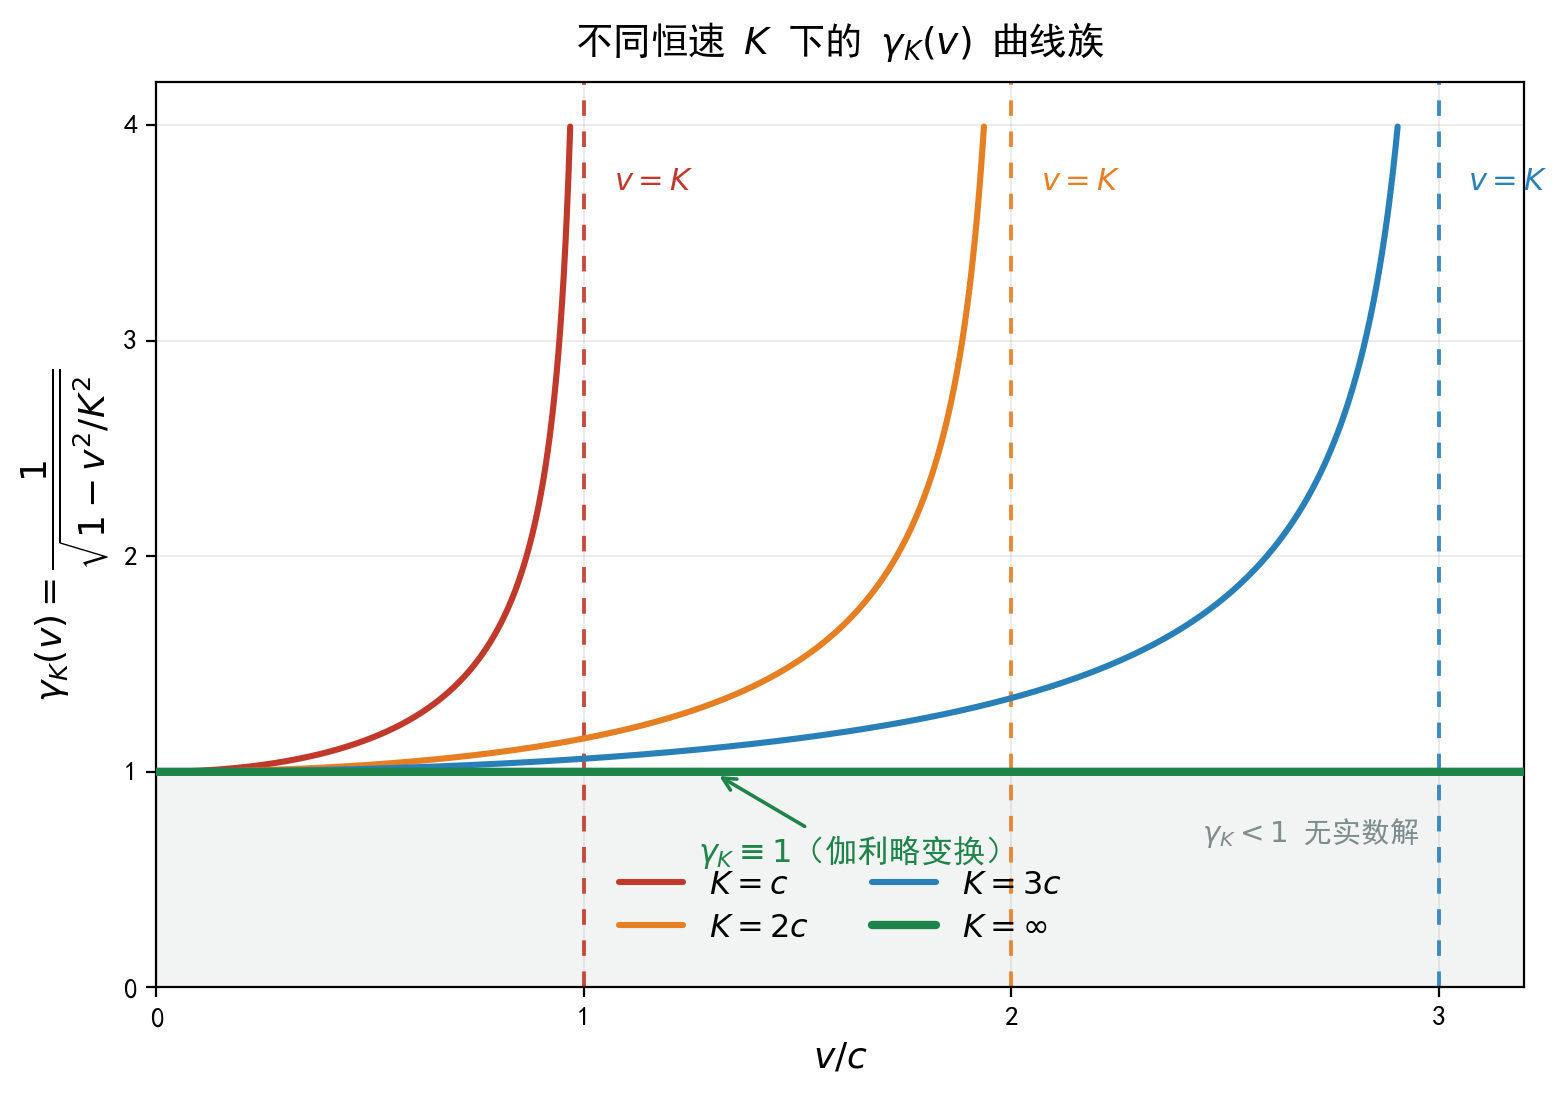
\includegraphics[width=0.86\linewidth,height=\textheight,keepaspectratio]{chapters/images/invariant-speed.png}

}

\caption{\label{fig-invariant-speed}不同 \(K\) 取值下的 \(\gamma_K(v)\)
曲线族}

\end{figure}%

图~\ref{fig-invariant-speed} 的横轴为 \(v/c\)，纵轴为
\(\gamma_K(v)\)，三条虚线分别标出三个有限 \(K\) 的发散位置
\(v=K\)。从图中可以直接读出三件事：

\begin{enumerate}
\def\labelenumi{\arabic{enumi}.}
\tightlist
\item
  \textbf{\(K=\infty\) 是水平线 \(\gamma_K\equiv1\)}，即伽利略变换；
\item
  \textbf{\(K\) 有限的曲线在 \(v\to K\) 处发散}，且 \(K\)
  越小，发散位置越靠左；
\item
  \textbf{\(K\)
  越小，曲线起翘越早}------即偏离伽利略行为的程度在更低的速度上就显现出来；反之
  \(K\) 越大，曲线在越宽的速度范围内贴近 \(1\)。
\end{enumerate}

\textbf{须说明}：该图只是 式~\ref{eq-isg-final}
的图像，不含超出该式的内容；它给出的是 \(\gamma\) 随 \(v/K\)
的变化，不涉及 \(K\) 应当取什么值。

\section{恒速群与狭义洛伦兹变换的关系}\label{sec-isg-not-same}

\subsection{形状相同，含义不同}\label{ux5f62ux72b6ux76f8ux540cux542bux4e49ux4e0dux540c}

式~\ref{eq-isg-final} 在 \(K=c\)
时，与狭义相对论中的洛伦兹变换\textbf{公式形状相同}。但二者不是同一个数学对象：

{\def\LTcaptype{none} % do not increment counter
\begin{longtable}[]{@{}
  >{\raggedright\arraybackslash}p{(\linewidth - 4\tabcolsep) * \real{0.3333}}
  >{\raggedright\arraybackslash}p{(\linewidth - 4\tabcolsep) * \real{0.3333}}
  >{\raggedright\arraybackslash}p{(\linewidth - 4\tabcolsep) * \real{0.3333}}@{}}
\toprule\noalign{}
\begin{minipage}[b]{\linewidth}\raggedright
\end{minipage} & \begin{minipage}[b]{\linewidth}\raggedright
恒速群 \(G_K\)
\end{minipage} & \begin{minipage}[b]{\linewidth}\raggedright
狭义洛伦兹变换
\end{minipage} \\
\midrule\noalign{}
\endhead
\bottomrule\noalign{}
\endlastfoot
对象 & 一族群，以 \(K\) 为参数 & 一个群，\(K\) 取定值 \(c\) \\
\(K\) 的地位 & 自由参数，取值待定 & 固定为 \(c\) \\
\(\infty\) 的处理 & \(K=\infty\) 是真取的极限 & \(c\) 有限，不取
\(\infty\) \\
\(t\) 的地位 & 随 \(K\) 而定：\(K<\infty\) 时随系变，\(K=\infty\) 时不变
& 随系改变 \\
\end{longtable}
}

\textbf{恒速群是一个族，狭义洛伦兹变换是这个族中的一个点。} 取 \(K=c\)
得到那个点；取 \(K=\infty\) 得到另一个点。

\subsection{为什么不能说「恒速群就是洛伦兹变换」}\label{ux4e3aux4ec0ux4e48ux4e0dux80fdux8bf4ux6052ux901fux7fa4ux5c31ux662fux6d1bux4f26ux5179ux53d8ux6362}

因为：

\begin{enumerate}
\def\labelenumi{\arabic{enumi}.}
\tightlist
\item
  \textbf{族不等于它的一个元素。} \(G_K\) 在 \(K=c\)
  处的值才是狭义洛伦兹变换。
\item
  \textbf{\(K=\infty\) 是真的取 \(\infty\)}，不是「把 \(c\)
  当作无穷」。这是两个完全不同的操作：一个是参数取极限，一个是把一个有限常数近似看作无穷。前者改变群的结构（庞加莱群收缩为伽利略群），后者只是一种数值近似。
\item
  \textbf{因此恒速群同时包含了两种时空结构的可能}，它在 \(K\)
  未定时，既不是纯粹的相对时空，也不是纯粹的绝对时空；选定 \(K\)
  之后才塌缩到其中一种。
\end{enumerate}

\textbf{这就是本章的核心命题：}

\begin{proposition}[恒速群是族，不是族中的一点]\protect\hypertarget{prp-isg-superposition}{}\label{prp-isg-superposition}

恒速群 \(G_K\) 是一个以 \(K\in(0,\infty]\) 为参数的群族，其中：

\begin{itemize}
\tightlist
\item
  \(K\) 有限（含 \(K=c\)）对应相对时空结构；
\item
  \(K=\infty\) 对应绝对时空结构（同时性不随系改变）；
\item
  \(K\to0\) 对应 Carroll 退化结构。
\end{itemize}

在 \(K\) 未取定之前，族本身不偏向其中任何一种

\end{proposition}

\section{与其他结构的对接}\label{sec-isg-others}

以下只陈述数学上的对应关系，不涉及物理判断。

\subsection{与波动力学方程}\label{ux4e0eux6ce2ux52a8ux529bux5b66ux65b9ux7a0b}

同一族群的表示论给出不同协变性要求的方程：

{\def\LTcaptype{none} % do not increment counter
\begin{longtable}[]{@{}
  >{\raggedright\arraybackslash}p{(\linewidth - 4\tabcolsep) * \real{0.3333}}
  >{\raggedright\arraybackslash}p{(\linewidth - 4\tabcolsep) * \real{0.3333}}
  >{\raggedright\arraybackslash}p{(\linewidth - 4\tabcolsep) * \real{0.3333}}@{}}
\toprule\noalign{}
\begin{minipage}[b]{\linewidth}\raggedright
\(K\)
\end{minipage} & \begin{minipage}[b]{\linewidth}\raggedright
协变性要求
\end{minipage} & \begin{minipage}[b]{\linewidth}\raggedright
相应的一阶／二阶方程
\end{minipage} \\
\midrule\noalign{}
\endhead
\bottomrule\noalign{}
\endlastfoot
\(K=c\) & 洛伦兹协变 & 克莱因--戈登方程、狄拉克方程 \\
\(K=\infty\) & 伽利略协变 & 薛定谔方程（严格表述用 Bargmann
群，即伽利略群的中央扩张）及 Lévy-Leblond 旋量方程 \\
\end{longtable}
}

\textbf{所以：量子力学的两类动力学方程可以纳入同一个参数化框架}，分别对应
\(K=\infty\) 与 \(K=c\) 两端，并通过群收缩相联系。

\subsection{与引力理论}\label{ux4e0eux5f15ux529bux7406ux8bba}

{\def\LTcaptype{none} % do not increment counter
\begin{longtable}[]{@{}
  >{\raggedright\arraybackslash}p{(\linewidth - 2\tabcolsep) * \real{0.5000}}
  >{\raggedright\arraybackslash}p{(\linewidth - 2\tabcolsep) * \real{0.5000}}@{}}
\toprule\noalign{}
\begin{minipage}[b]{\linewidth}\raggedright
\(K\)
\end{minipage} & \begin{minipage}[b]{\linewidth}\raggedright
几何结构
\end{minipage} \\
\midrule\noalign{}
\endhead
\bottomrule\noalign{}
\endlastfoot
\(K=c\) & 洛伦兹几何，爱因斯坦场方程 \\
\(K=\infty\) & Newton--Cartan
几何（退化度规：时间一形式与空间度规分离） \\
\end{longtable}
}

两者同样由收缩相联系。\(K=\infty\) 一端并非空缺，而是有对应的几何构造。

\subsection{与黑洞：不兼容}\label{ux4e0eux9ed1ux6d1eux4e0dux517cux5bb9}

黑洞的现代定义是\textbf{事件视界}：时空因果结构中的单向膜，即光锥向内倾斜到不存在任何向外的未来方向的区域。

这个定义\textbf{直接依赖特征速度有限}：

\begin{itemize}
\tightlist
\item
  逃逸速度 \(v_{\text{esc}}=\sqrt{2GM/r}\)；
\item
  令 \(v_{\text{esc}}=K\)，得临界半径 \(r=2GM/K^{2}\)；
\item
  当 \(K=c\) 时，即 \(r_s=2GM/c^{2}\)，其内侧为事件视界。
\end{itemize}

\textbf{取 \(K=\infty\) 时}：

\begin{itemize}
\tightlist
\item
  允许的速度无上限（\(|v|<K\to\infty\)），任何有限速度都能逃逸；
\item
  光锥不再界定因果可达范围；
\item
  \textbf{不存在单向膜，因而不存在事件视界}。
\end{itemize}

需要区分两层：

{\def\LTcaptype{none} % do not increment counter
\begin{longtable}[]{@{}
  >{\raggedright\arraybackslash}p{(\linewidth - 2\tabcolsep) * \real{0.5000}}
  >{\raggedright\arraybackslash}p{(\linewidth - 2\tabcolsep) * \real{0.5000}}@{}}
\toprule\noalign{}
\begin{minipage}[b]{\linewidth}\raggedright
黑洞的定义
\end{minipage} & \begin{minipage}[b]{\linewidth}\raggedright
与 \(K=\infty\) 的关系
\end{minipage} \\
\midrule\noalign{}
\endhead
\bottomrule\noalign{}
\endlastfoot
逃逸速度 \(\ge c\) 的天体（暗星） &
\textbf{可以存在}（若另行规定光以有限速率 \(c\) 传播） \\
事件视界（因果结构中的单向膜） & \textbf{不存在} \\
\end{longtable}
}

前者的障碍是\textbf{动力学}的（光跑得不够快，被引力拉回，像抛出的球）；后者的障碍是\textbf{因果结构}的（时空本身不提供向外的未来方向）。\textbf{\(K=\infty\)
的框架只容得下前者。}

（顺带一句：这正是第 章节~\ref{sec-two-source-field} 章公设 A1+A2
所处的情形------坐标变换取伽利略式（\(K=\infty\)），同时另行规定光在静系以有限速率
\(c\) 传播。）

\subsection{汇总}\label{ux6c47ux603b}

\begin{longtable}[]{@{}
  >{\raggedright\arraybackslash}p{(\linewidth - 8\tabcolsep) * \real{0.2000}}
  >{\raggedright\arraybackslash}p{(\linewidth - 8\tabcolsep) * \real{0.2000}}
  >{\raggedright\arraybackslash}p{(\linewidth - 8\tabcolsep) * \real{0.2000}}
  >{\raggedright\arraybackslash}p{(\linewidth - 8\tabcolsep) * \real{0.2000}}
  >{\raggedright\arraybackslash}p{(\linewidth - 8\tabcolsep) * \real{0.2000}}@{}}
\caption{\(K\)
的取值与具体结构的对照}\label{tbl-isg-applications}\tabularnewline
\toprule\noalign{}
\begin{minipage}[b]{\linewidth}\raggedright
\(K\)
\end{minipage} & \begin{minipage}[b]{\linewidth}\raggedright
协变性要求
\end{minipage} & \begin{minipage}[b]{\linewidth}\raggedright
波动力学
\end{minipage} & \begin{minipage}[b]{\linewidth}\raggedright
引力几何
\end{minipage} & \begin{minipage}[b]{\linewidth}\raggedright
事件视界
\end{minipage} \\
\midrule\noalign{}
\endfirsthead
\toprule\noalign{}
\begin{minipage}[b]{\linewidth}\raggedright
\(K\)
\end{minipage} & \begin{minipage}[b]{\linewidth}\raggedright
协变性要求
\end{minipage} & \begin{minipage}[b]{\linewidth}\raggedright
波动力学
\end{minipage} & \begin{minipage}[b]{\linewidth}\raggedright
引力几何
\end{minipage} & \begin{minipage}[b]{\linewidth}\raggedright
事件视界
\end{minipage} \\
\midrule\noalign{}
\endhead
\bottomrule\noalign{}
\endlastfoot
\(c\) & 洛伦兹协变 & 克莱因--戈登、狄拉克 & 洛伦兹几何（GR） &
有（\(r_s=2GM/c^{2}\)） \\
有限且 \(\neq c\) & 以 \(K\) 为不变速度的协变 & 同族方程（\(c\) 替换为
\(K\)） & 同族几何 & 有（\(r=2GM/K^{2}\)） \\
\(\infty\) & 伽利略协变 & 薛定谔（Bargmann 群） & Newton--Cartan &
\textbf{无} \\
\(0\) & Carroll 型 & 退化 & 退化 & 无 \\
\end{longtable}

\section{结论}\label{sec-isg-conclusion}

\begin{longtable}[]{@{}
  >{\raggedright\arraybackslash}p{(\linewidth - 2\tabcolsep) * \real{0.5000}}
  >{\raggedright\arraybackslash}p{(\linewidth - 2\tabcolsep) * \real{0.5000}}@{}}
\caption{各命题及其依据}\label{tbl-isg-conclusion}\tabularnewline
\toprule\noalign{}
\begin{minipage}[b]{\linewidth}\raggedright
命题
\end{minipage} & \begin{minipage}[b]{\linewidth}\raggedright
依据
\end{minipage} \\
\midrule\noalign{}
\endfirsthead
\toprule\noalign{}
\begin{minipage}[b]{\linewidth}\raggedright
命题
\end{minipage} & \begin{minipage}[b]{\linewidth}\raggedright
依据
\end{minipage} \\
\midrule\noalign{}
\endhead
\bottomrule\noalign{}
\endlastfoot
变换构成以 \(K\) 为参数的群族 & A1---A4（式~\ref{eq-isg-final}） \\
\(t'=t\) 是 \(K=\infty\) 的推论 & 式~\ref{eq-isg-galilei} \\
\(K=\infty\) 是真取 \(\infty\)，不是拿 \(c\) 充当无穷 & \(\gamma\to1\)
与 \(v/K^{2}\to0\) 同时成立 \\
恒速群是族，狭义洛伦兹变换是族中一点 &
命题~\ref{prp-isg-superposition} \\
量子力学的两类方程分别对应 \(K=\infty\) 与 \(K=c\) & 群表示与收缩 \\
\(K=\infty\) 下无事件视界 & 光锥退化，无单向膜 \\
\end{longtable}

\textbf{一句话}：把「存在恒速
\(K\)」作为唯一公设，得到的不是某一种时空结构，而是\textbf{一族时空结构}；伽利略变换是这族在
\(K=\infty\) 处的极限（不变时间随之作为推论出现），狭义洛伦兹变换是
\(K=c\) 处的取值。族本身在 \(K\) 未定时不偏向任何一端。

\bookmarksetup{startatroot}

\chapter{恒速场群}\label{sec-invariant-speed-field-group}

\section{本章的范围}\label{sec-ifg-scope}

\textbf{一句话}：本章把第 章节~\ref{sec-invariant-speed-group} 章的常数
\(K\) 换成时空上的函数
\(K(p)\)，然后问三个问题------逐点的群还在不在、跨点的复合还在不在、它究竟能给出多少几何与表示论。

本章只讨论数学对象之间的对应关系。

三个问题的答案先列出，下文逐一给出依据：

{\def\LTcaptype{none} % do not increment counter
\begin{longtable}[]{@{}
  >{\raggedright\arraybackslash}p{(\linewidth - 4\tabcolsep) * \real{0.3333}}
  >{\raggedright\arraybackslash}p{(\linewidth - 4\tabcolsep) * \real{0.3333}}
  >{\raggedright\arraybackslash}p{(\linewidth - 4\tabcolsep) * \real{0.3333}}@{}}
\toprule\noalign{}
\begin{minipage}[b]{\linewidth}\raggedright
问题
\end{minipage} & \begin{minipage}[b]{\linewidth}\raggedright
答案
\end{minipage} & \begin{minipage}[b]{\linewidth}\raggedright
依据
\end{minipage} \\
\midrule\noalign{}
\endhead
\bottomrule\noalign{}
\endlastfoot
逐点的群还在不在 & 在。每点一个 \(G_{K(p)}\) &
小节~\ref{sec-ifg-fiber} \\
跨点的复合还在不在 & 不在，需要额外的联络 & 小节~\ref{sec-ifg-cross} \\
能给出多少几何 & 在受限约定下能给出曲率，但给不出一般度规 &
小节~\ref{sec-ifg-gr} \\
\end{longtable}
}

\section{恒速场}\label{sec-ifg-field}

\subsection{定义}\label{ux5b9aux4e49}

\begin{definition}[恒速场]\protect\hypertarget{def-ifg-field}{}\label{def-ifg-field}

设 \(M\) 是一个 \(n+1\) 维光滑流形。称函数

\[
K:M\longrightarrow(0,\infty]
\]

为 \(M\) 上的\textbf{恒速场}。

\end{definition}

在每点 \(p\in M\)，把 \(K(p)\) 的值代入第
章节~\ref{sec-invariant-speed-group} 章的
式~\ref{eq-isg-final}，得到一个作用在切空间 \(T_pM\)
上的线性变换群，记为 \(G_{K(p)}\)。

\subsection{这不是一个群}\label{ux8fd9ux4e0dux662fux4e00ux4e2aux7fa4}

\textbf{这一点必须说清楚}：把所有点上的 \(G_{K(p)}\)
放在一起，得到的\textbf{不是}一个群。

理由是：群的运算（复合）要求两个元素作用在同一个集合上。\(\Lambda\in G_{K(p)}\)
作用在 \(T_pM\) 上，\(\Lambda'\in G_{K(q)}\) 作用在 \(T_qM\) 上。当
\(p\neq q\) 时这是两个不同的向量空间，\(\Lambda'\circ\Lambda\)
没有定义。

数学上这类对象的名字是\textbf{群丛}（逐点指定的群所构成的丛）。为避免与其他领域的同名用法混淆，本章称它为\textbf{恒速场群}。

\subsection{逐点的三个端点}\label{ux9010ux70b9ux7684ux4e09ux4e2aux7aefux70b9}

第 章节~\ref{sec-invariant-speed-group} 章的三个端点现在逐点化：

{\def\LTcaptype{none} % do not increment counter
\begin{longtable}[]{@{}lll@{}}
\toprule\noalign{}
\(K(p)\) 的取值 & \(p\) 点处的群 & 该点特征 \\
\midrule\noalign{}
\endhead
\bottomrule\noalign{}
\endlastfoot
有限（含 \(K=c\)） & 洛伦兹型 & 该点有有限的不变速度 \\
\(\infty\) & 伽利略型 & 该点时间分量不变 \\
\(\to0\) & Carroll 型 & 该点空间分量不变（需重新参数化） \\
\end{longtable}
}

\textbf{注意}：\(K\) 场可以在不同点取不同类型的端点值。这是常数 \(K\)
情形下不存在的新现象，见 小节~\ref{sec-ifg-interface}。

\section{纤维内：逐点闭合}\label{sec-ifg-fiber}

\subsection{命题}\label{ux547dux9898}

\begin{proposition}[逐点群]\protect\hypertarget{prp-ifg-fiber}{}\label{prp-ifg-fiber}

对每一点 \(p\)，\(G_{K(p)}\) 是群。

\end{proposition}

\textbf{证明}：第 章节~\ref{sec-invariant-speed-group} 章推导
式~\ref{eq-isg-final} 的每一步，只用到了「该点的 \(K\)
值」这一个信息，没有用到「\(K\) 在所有点相同」。逐步核对：

\begin{enumerate}
\def\labelenumi{\arabic{enumi}.}
\tightlist
\item
  第一步至第三步（定出
  \(C=-vA\)、\(D=A\)）：只用到线性性与空间反射，不含 \(K\)；
\item
  第四步（定出 \(\beta=-v/K^{2}\)）：只用到 \(p\) 点处速度为 \(K(p)\)
  的变换行为；
\item
  第五步（定出 \(A(v)=1/\sqrt{1-v^{2}/K^{2}}\)）：只用到同一个 \(K\)
  值下的群闭合。
\end{enumerate}

因此把 \(K\) 换成 \(K(p)\)，全部推导逐字成立：在 \(p\) 点，\(G_{K(p)}\)
对复合封闭、含恒等元、每个元素可逆。

\textbf{此命题的适用范围}：只限于\textbf{同一根纤维内}（同一切空间上）的复合。跨纤维的复合见
小节~\ref{sec-ifg-cross}。

\subsection{齐次群与非齐次群}\label{ux9f50ux6b21ux7fa4ux4e0eux975eux9f50ux6b21ux7fa4}

第 章节~\ref{sec-invariant-speed-group} 章的 \(G_K\) 只含 boost（参数
\(v\)），是\textbf{齐次}的------它保持原点不动。要谈完整的李代数结构，还需把平移纳入。

加入时间平移 \(a\) 与空间平移 \(b\)，得\textbf{非齐次恒速群}
\(IG_K\)，作用于 \((t,x)\)：

\[
t'=A(v)\Bigl(t-\frac{v\,x}{K^{2}}\Bigr)+a,\qquad
x'=A(v)\,(x-vt)+b
\]

在 1+1 维、\(K\) 常数时，这是 \(3\) 参数群。

\subsection{\texorpdfstring{生成元与结构常数（\(K\)
常数）}{生成元与结构常数（K 常数）}}\label{ux751fux6210ux5143ux4e0eux7ed3ux6784ux5e38ux6570k-ux5e38ux6570}

对 \(v\) 在 \(v=0\) 处求导。由 式~\ref{eq-isg-final} 记
\(A(v)=\bigl(1-v^{2}/K^{2}\bigr)^{-1/2}\)，有
\(A(0)=1\)、\(A'(0)=0\)（\(A\) 是 \(v\) 的偶函数），故

\[
\left.\frac{\partial t'}{\partial v}\right|_{v=0}=-\frac{x}{K^{2}},\qquad
\left.\frac{\partial x'}{\partial v}\right|_{v=0}=-t
\]

即 boost 生成元为向量场

\[
B=-\frac{x}{K^{2}}\,\partial_t-t\,\partial_x
\]

另两个生成元为平移：\(H=\partial_t\)、\(P=\partial_x\)。

\textbf{逐项计算李括号}（记
\(B^{t}=-x/K^{2}\)、\(B^{x}=-t\)；\(H^{t}=1\)、\(H^{x}=0\)；\(P^{t}=0\)、\(P^{x}=1\)）：

\emph{\([B,H]\) 的时间分量}：

\[
[B,H]^{t}=B^{j}\partial_j H^{t}-H^{j}\partial_j B^{t}
=0-\partial_t\!\left(-\frac{x}{K^{2}}\right)=0
\]

（\(K\) 为常数，故 \(\partial_t(x/K^{2})=0\)。）

\emph{\([B,H]\) 的空间分量}：

\[
[B,H]^{x}=B^{j}\partial_j H^{x}-H^{j}\partial_j B^{x}
=0-\partial_t(-t)=1
\]

故

\begin{equation}\protect\phantomsection\label{eq-ifg-BH}{
[B,H]=P
}\end{equation}

\emph{\([B,P]\) 的时间分量}：

\[
[B,P]^{t}=B^{j}\partial_j P^{t}-P^{j}\partial_j B^{t}
=0-\partial_x\!\left(-\frac{x}{K^{2}}\right)=\frac{1}{K^{2}}
\]

\emph{\([B,P]\) 的空间分量}：

\[
[B,P]^{x}=B^{j}\partial_j P^{x}-P^{j}\partial_j B^{x}
=0-\partial_x(-t)=0
\]

故

\begin{equation}\protect\phantomsection\label{eq-ifg-BP}{
[B,P]=\frac{1}{K^{2}}\,H
}\end{equation}

另有显然的 \([H,P]=0\)。

\subsection{由此得到的一个硬结论}\label{ux7531ux6b64ux5f97ux5230ux7684ux4e00ux4e2aux786cux7ed3ux8bba}

\textbf{\(K\) 在李代数中只出现在结构常数 \(1/K^{2}\) 的位置上。} 于是：

{\def\LTcaptype{none} % do not increment counter
\begin{longtable}[]{@{}lll@{}}
\toprule\noalign{}
\(K\) & \([B,P]\) & 李代数 \\
\midrule\noalign{}
\endhead
\bottomrule\noalign{}
\endlastfoot
有限 & \(\dfrac{1}{K^{2}}H\neq0\) & 庞加莱型 \\
\(\infty\) & \(0\) & 伽利略型 \\
\end{longtable}
}

\textbf{这两个李代数不同构}------一个有非零结构常数，一个为零。这是第
章节~\ref{sec-invariant-speed-group}
章「两支底层不同」这句话在李代数层面的证明；而群收缩在李代数层面就是一句

\[
\frac{1}{K^{2}}\longrightarrow 0\qquad (K\to\infty)
\]

\subsection{结构常数变场}\label{ux7ed3ux6784ux5e38ux6570ux53d8ux573a}

把 \(K\) 换成 \(K(p)\)，由 式~\ref{eq-ifg-BH} 与
式~\ref{eq-ifg-BP}，每点的结构常数为

\[
[B,P]_{p}=\frac{1}{K(p)^{2}}\,H
\]

\textbf{结构常数成为时空上的函数。}
这个对象的数学名字是\textbf{李代数丛}：每根纤维上是一个李代数，不同纤维上的李代数由不同的结构常数刻画。

\section{跨纤维：复合失效}\label{sec-ifg-cross}

\subsection{内禀的论证}\label{ux5185ux7980ux7684ux8bbaux8bc1}

\(\Lambda\in G_{K(p)}\) 与 \(\Lambda'\in G_{K(q)}\)
作用在\textbf{不同的向量空间}上。要让它们复合，必须先指定一个把 \(T_qM\)
搬到 \(T_pM\) 的线性同构------这就是\textbf{联络}。

\textbf{联络不是由 \(K\) 场给出的。} \(K\)
场只说「每点用哪个群」，不说「各点之间怎么缝合」。这是两个互相独立的结构。

\subsection{坐标下的显式演示}\label{ux5750ux6807ux4e0bux7684ux663eux5f0fux6f14ux793a}

上面的论证是定性的。要看出「失效」具体是什么形状，可以在一个坐标卡里做显式计算。

\textbf{须说明这一步的坐标依赖性}：下面把逐点的生成元当作向量场来用，这只有在取定坐标卡、使「位置向量」有意义时才成立，因此它不是内禀的。它的作用只是把失效的量显式写出来。

取 1+1 维，坐标 \((t,x)\)。把 \(B\) 的分量中的 \(K\) 换成 \(K(t,x)\)：

\[
B^{t}=-\frac{x}{K(t,x)^{2}},\qquad B^{x}=-t
\]

重算括号。

\emph{\([B,H]\) 的时间分量}：

\[
[B,H]^{t}=0-\partial_t\!\left(-\frac{x}{K^{2}}\right)
=x\,\partial_t\!\left(K^{-2}\right)
=x\cdot\left(-2K^{-3}\,\partial_tK\right)
=-\frac{2x}{K^{3}}\,\partial_tK
\]

空间分量同前为 \(1\)，故

\begin{equation}\protect\phantomsection\label{eq-ifg-BH-field}{
[B,H]=P-\frac{2x\,\partial_tK}{K^{3}}\,H
}\end{equation}

\emph{\([B,P]\) 的时间分量}：

\[
[B,P]^{t}=0-\partial_x\!\left(-\frac{x}{K^{2}}\right)
=\partial_x\!\left(x\,K^{-2}\right)
=K^{-2}+x\left(-2K^{-3}\,\partial_xK\right)
\]

空间分量同前为 \(0\)，故

\begin{equation}\protect\phantomsection\label{eq-ifg-BP-field}{
[B,P]=\left(\frac{1}{K^{2}}-\frac{2x\,\partial_xK}{K^{3}}\right)H
}\end{equation}

\subsection{两个后果}\label{ux4e24ux4e2aux540eux679c}

\textbf{后果一：不再闭合。} 式~\ref{eq-ifg-BP-field} 的右端是「函数」乘
\(H\)，而不是「常数」乘 \(H\)。因此在实常系数下由 \(\{H,P,B\}\) 张成的
\(3\) 维空间，对李括号\textbf{不封闭}：

\begin{itemize}
\tightlist
\item
  \(K\) 常数时，右端系数为 \(1/K^{2}\)，是常数，闭合；
\item
  \(K\) 非常数时，右端系数含 \(\partial_xK\)，不是常数，漏出这个 \(3\)
  维空间。
\end{itemize}

\textbf{后果二：多出来的项正比于 \(\partial K\)。} 由
式~\ref{eq-ifg-BH-field} 与 式~\ref{eq-ifg-BP-field}，两个多出项都形如

\[
\frac{x\,\partial_\mu K}{K^{3}}
=\frac{\partial_\mu K}{K}\cdot\frac{x}{K^{2}}
\]

即都正比于 \(\partial_\mu K/K\)。

\textbf{这一点很关键}：小节~\ref{sec-ifg-connection}
将算出，在对角约定下 Levi-Civita 联络的 Christoffel 符号恰好是
\(\partial_\mu K/K\) 型。也就是说，\textbf{联络所做的正是吸收这一类项}。

\section{联络：从群丛到几何}\label{sec-ifg-connection}

\subsection{补上联络之后}\label{ux8865ux4e0aux8054ux7edcux4e4bux540e}

一旦补上联络，就可以谈曲率。但联络有无穷多种选法，\(K\)
场并不挑出其中任何一种。

\textbf{本节做一件事}：取一个\textbf{约定}（下文的「对角约定」），使联络由度规唯一确定，从而把联络也用
\(K\) 场表达出来。这样得到一个可以完整算到底的例子。这个约定的局限在
小节~\ref{sec-ifg-gr} 中说明。

\subsection{对角约定}\label{ux5bf9ux89d2ux7ea6ux5b9a}

\begin{definition}[对角约定]\protect\hypertarget{def-ifg-diagonal}{}\label{def-ifg-diagonal}

在 \(n+1\) 维流形上取度规

\begin{equation}\protect\phantomsection\label{eq-ifg-metric}{
\mathrm{d}s^{2}=K^{2}\,\mathrm{d}t^{2}-\delta_{ij}\,\mathrm{d}x^{i}\mathrm{d}x^{j}
}\end{equation}

其中 \(K=K(t,x^{1},\dots,x^{n})\) 即恒速场，\(\delta_{ij}\) 为欧氏度规。

\end{definition}

\textbf{与第 章节~\ref{sec-invariant-speed-group} 章的一致性检验}：\(K\)
为常数时，式~\ref{eq-ifg-metric} 的二次型正是
\(Q_K=K^{2}t^{2}-\lvert\mathbf{x}\rvert^{2}\)，即该章的不变量。

度规分量及其逆：

\[
g_{00}=K^{2},\qquad g_{ij}=-\delta_{ij},\qquad g_{0i}=0
\]

\[
g^{00}=\frac{1}{K^{2}},\qquad g^{ij}=-\delta^{ij},\qquad g^{0i}=0
\]

\textbf{注意 \(g_{ij}=-\delta_{ij}\) 是常数}，故
\(\partial_\mu g_{ij}=0\)；唯一的非零导数是
\(\partial_\mu g_{00}=2K\,\partial_\mu K\)。这是下面所有计算得以大幅简化的原因。

\subsection{Christoffel
符号（逐项）}\label{christoffel-ux7b26ux53f7ux9010ux9879}

\[
\Gamma^{\rho}_{\mu\nu}=\frac{1}{2}g^{\rho\sigma}
\bigl(\partial_\mu g_{\nu\sigma}+\partial_\nu g_{\mu\sigma}-\partial_\sigma g_{\mu\nu}\bigr)
\]

逐项代入（\(\rho=0\) 时求和只剩 \(\sigma=0\)；\(\rho=k\) 时只剩
\(\sigma=l\)）。

\textbf{(a) \(\Gamma^{0}_{00}\)}

\[
\Gamma^{0}_{00}=\frac{1}{2}g^{00}\bigl(\partial_0g_{00}+\partial_0g_{00}-\partial_0g_{00}\bigr)
=\frac{1}{2}\cdot\frac{1}{K^{2}}\cdot\bigl(2K\,\partial_0K\bigr)
=\frac{\partial_0K}{K}
\]

\textbf{(b) \(\Gamma^{0}_{0i}=\Gamma^{0}_{i0}\)}

\[
\Gamma^{0}_{0i}=\frac{1}{2}g^{00}\bigl(\partial_0g_{i0}+\partial_ig_{00}-\partial_0g_{i0}\bigr)
=\frac{1}{2}\cdot\frac{1}{K^{2}}\cdot\bigl(2K\,\partial_iK\bigr)
=\frac{\partial_iK}{K}
\]

\textbf{(c) \(\Gamma^{0}_{ij}\)}

\[
\Gamma^{0}_{ij}=\frac{1}{2}g^{00}\bigl(\partial_ig_{j0}+\partial_jg_{i0}-\partial_0g_{ij}\bigr)=0
\]

（前两项含 \(g_{i0}=0\)，第三项含 \(\partial_0g_{ij}=0\)。）

\textbf{(d) \(\Gamma^{k}_{00}\)}

\[
\Gamma^{k}_{00}=\frac{1}{2}g^{kl}\bigl(\partial_0g_{0l}+\partial_0g_{0l}-\partial_lg_{00}\bigr)
=\frac{1}{2}\bigl(-\delta^{kl}\bigr)\bigl(-2K\,\partial_lK\bigr)
=K\,\partial_kK
\]

\textbf{(e) \(\Gamma^{k}_{0i}\) 与 \(\Gamma^{k}_{ij}\)}

\[
\Gamma^{k}_{0i}=\frac{1}{2}g^{kl}\bigl(\partial_0g_{il}+\partial_ig_{0l}-\partial_lg_{0i}\bigr)=0
\]

\[
\Gamma^{k}_{ij}=\frac{1}{2}g^{kl}\bigl(\partial_ig_{jl}+\partial_jg_{il}-\partial_lg_{ij}\bigr)=0
\]

\textbf{汇总}（其余为零）：

\begin{equation}\protect\phantomsection\label{eq-ifg-christoffel}{
\Gamma^{0}_{00}=\frac{\partial_0K}{K},\qquad
\Gamma^{0}_{0i}=\Gamma^{0}_{i0}=\frac{\partial_iK}{K},\qquad
\Gamma^{k}_{00}=K\,\partial_kK
}\end{equation}

\textbf{关键观察}：所有非零 Christoffel 符号都形如
\(\partial_\mu K/K\)，与 小节~\ref{sec-ifg-cross} 中「多出来的项」同型。

\subsection{Ricci 张量（逐项）}\label{ricci-ux5f20ux91cfux9010ux9879}

\[
R_{\sigma\nu}=\partial_\rho\Gamma^{\rho}_{\nu\sigma}
-\partial_\nu\Gamma^{\rho}_{\rho\sigma}
+\Gamma^{\rho}_{\rho\lambda}\Gamma^{\lambda}_{\nu\sigma}
-\Gamma^{\rho}_{\nu\lambda}\Gamma^{\lambda}_{\rho\sigma}
\]

记
\(\lvert\nabla K\rvert^{2}:=\sum_k(\partial_kK)^{2}\)，\(\Delta K:=\sum_k\partial_k\partial_kK\)（空间拉普拉斯），\(K_0:=\partial_0K\)。

\textbf{(a) \(R_{00}\)} 的四项分别为：

\emph{第一项}：

\[
\partial_\rho\Gamma^{\rho}_{00}
=\partial_0\Gamma^{0}_{00}+\partial_k\Gamma^{k}_{00}
=\partial_0\!\left(\frac{K_0}{K}\right)+\partial_k\bigl(K\,\partial_kK\bigr)
\]

\[
=\left(\frac{\partial_0^{2}K}{K}-\frac{K_0^{2}}{K^{2}}\right)+\lvert\nabla K\rvert^{2}+K\,\Delta K
\]

\emph{第二项}：

\[
\partial_0\Gamma^{\rho}_{\rho0}
=\partial_0\bigl(\Gamma^{0}_{00}+\Gamma^{k}_{k0}\bigr)
=\partial_0\!\left(\frac{K_0}{K}+0\right)
=\frac{\partial_0^{2}K}{K}-\frac{K_0^{2}}{K^{2}}
\]

\emph{第三项}（\(\lambda\) 取 \(0\) 与 \(i\) 两类）：

\[
\Gamma^{\rho}_{\rho\lambda}\Gamma^{\lambda}_{00}
=\frac{K_0}{K}\cdot\frac{K_0}{K}
+\sum_i\frac{\partial_iK}{K}\cdot\bigl(K\,\partial_iK\bigr)
=\frac{K_0^{2}}{K^{2}}+\lvert\nabla K\rvert^{2}
\]

\emph{第四项}（\((\rho,\lambda)\) 的四种组合
\((0,0)\)、\((0,i)\)、\((k,0)\)、\((k,i)\)）：

\[
\Gamma^{\rho}_{0\lambda}\Gamma^{\lambda}_{\rho0}
=\frac{K_0}{K}\cdot\frac{K_0}{K}
+\frac{\partial_iK}{K}\cdot\bigl(K\,\partial_iK\bigr)
+\bigl(K\,\partial_kK\bigr)\cdot\frac{\partial_kK}{K}
+0
=\frac{K_0^{2}}{K^{2}}+2\lvert\nabla K\rvert^{2}
\]

\emph{四项相减}（第一项 − 第二项 + 第三项 − 第四项）：

\[
R_{00}=\bigl[\lvert\nabla K\rvert^{2}+K\,\Delta K\bigr]
+\bigl[\lvert\nabla K\rvert^{2}\bigr]
-\bigl[2\lvert\nabla K\rvert^{2}\bigr]
=K\,\Delta K
\]

其中含 \(\partial_0^{2}K\) 与 \(K_0^{2}\)
的项在第一、二项之间精确抵消。故

\[
\boxed{R_{00}=K\,\Delta K}
\]

\textbf{(b) \(R_{ij}\)} 的四项分别为：

第一项 \(\partial_\rho\Gamma^{\rho}_{ij}=0\)（因
\(\Gamma^{0}_{ij}=\Gamma^{k}_{ij}=0\)）；第三项
\(\Gamma^{\rho}_{\rho\lambda}\Gamma^{\lambda}_{ij}=0\)（因
\(\Gamma^{\lambda}_{ij}=0\)）。

\emph{第二项}：

\[
\partial_j\Gamma^{\rho}_{\rho i}
=\partial_j\!\left(\frac{\partial_iK}{K}\right)
=\frac{\partial_i\partial_jK}{K}-\frac{\partial_iK\,\partial_jK}{K^{2}}
\]

\emph{第四项}（只有 \((\rho,\lambda)=(0,0)\) 非零）：

\[
\Gamma^{\rho}_{j\lambda}\Gamma^{\lambda}_{\rho i}
=\Gamma^{0}_{j0}\,\Gamma^{0}_{0i}
=\frac{\partial_jK}{K}\cdot\frac{\partial_iK}{K}
\]

\emph{四项相减}：

\[
R_{ij}
=0-\left(\frac{\partial_i\partial_jK}{K}-\frac{\partial_iK\,\partial_jK}{K^{2}}\right)
+0-\frac{\partial_iK\,\partial_jK}{K^{2}}
=-\frac{\partial_i\partial_jK}{K}
\]

\[
\boxed{R_{ij}=-\frac{\partial_i\partial_jK}{K}}
\]

\textbf{(c) \(R_{0i}\)} 的四项分别为：

\[
\partial_\rho\Gamma^{\rho}_{0i}
=\partial_0\!\left(\frac{\partial_iK}{K}\right)
=\frac{\partial_0\partial_iK}{K}-\frac{\partial_iK\,K_0}{K^{2}}
\]

\[
\partial_i\Gamma^{\rho}_{\rho0}
=\partial_i\!\left(\frac{K_0}{K}\right)
=\frac{\partial_0\partial_iK}{K}-\frac{K_0\,\partial_iK}{K^{2}}
\]

\[
\Gamma^{\rho}_{\rho\lambda}\Gamma^{\lambda}_{0i}=\frac{K_0}{K}\cdot\frac{\partial_iK}{K},\qquad
\Gamma^{\rho}_{i\lambda}\Gamma^{\lambda}_{\rho0}=\frac{\partial_iK}{K}\cdot\frac{K_0}{K}
\]

四项相减时，两类项两两精确抵消：

\[
\boxed{R_{0i}=0}
\]

\subsection{Ricci 标量}\label{ricci-ux6807ux91cf}

\[
R=g^{00}R_{00}+g^{ij}R_{ij}
=\frac{1}{K^{2}}\bigl(K\,\Delta K\bigr)
+\bigl(-\delta^{ij}\bigr)\left(-\frac{\partial_i\partial_jK}{K}\right)
\]

\[
=\frac{\Delta K}{K}+\frac{\delta^{ij}\partial_i\partial_jK}{K}
=\frac{\Delta K}{K}+\frac{\Delta K}{K}
\]

\begin{equation}\protect\phantomsection\label{eq-ifg-R}{
\boxed{R=\frac{2\,\Delta K}{K}}
}\end{equation}

\textbf{这个结果与空间维数 \(n\) 无关。}

\textbf{自检}：\(K\) 为常数 ⟹ \(\Delta K=0\) ⟹ \(R=0\)，平坦。✓

\textbf{一个直接的推论}：\(R\) 只含\textbf{空间}二阶导数，不含
\(\partial_0^{2}K\)。也就是说，在这个约定下 \(K\)
场的时间依赖不产生曲率。这与一件可以直接验证的事一致：若 \(K=K(t)\)
只依赖 \(t\)，作坐标变换 \(\tilde t=\int^{t}K(s)\,\mathrm{d}s\)，则
\(K^{2}\mathrm{d}t^{2}=\mathrm{d}\tilde t^{2}\)，式~\ref{eq-ifg-metric}
化为 Minkowski 度规。

\subsection{Einstein 张量}\label{einstein-ux5f20ux91cf}

\[
G_{\mu\nu}=R_{\mu\nu}-\frac{1}{2}R\,g_{\mu\nu}
\]

逐项代入：

\[
G_{00}=K\,\Delta K-\frac{1}{2}\cdot\frac{2\,\Delta K}{K}\cdot K^{2}
=K\,\Delta K-K\,\Delta K=0
\]

\[
G_{0i}=0-\frac{1}{2}R\cdot 0=0
\]

\begin{equation}\protect\phantomsection\label{eq-ifg-G}{
G_{ij}=-\frac{\partial_i\partial_jK}{K}
-\frac{1}{2}\cdot\frac{2\,\Delta K}{K}\cdot\bigl(-\delta_{ij}\bigr)
=\frac{\Delta K\,\delta_{ij}-\partial_i\partial_jK}{K}
}\end{equation}

\[
\boxed{G_{00}=0,\qquad G_{0i}=0,\qquad
G_{ij}=\frac{\Delta K\,\delta_{ij}-\partial_i\partial_jK}{K}}
\]

\subsection{真空解}\label{ux771fux7a7aux89e3}

由 式~\ref{eq-ifg-G}，真空要求 \(G_{ij}=0\)，即

\[
\partial_i\partial_jK=\Delta K\,\delta_{ij}
\]

对 \(i=j\) 求和（\(n\) 个空间维，\(\delta_{ii}=n\)）：

\[
\Delta K=\Delta K\cdot n
\quad\Longrightarrow\quad
(n-1)\,\Delta K=0
\]

当 \(n\geq2\) 时得 \(\Delta K=0\)，代回得
\(\partial_i\partial_jK=0\)。故 \(K\) 对空间坐标是\textbf{仿射}的：

\begin{equation}\protect\phantomsection\label{eq-ifg-vacuum}{
\boxed{K(t,\mathbf{x})=a(t)+b_i(t)\,x^{i}}
}\end{equation}

即：在对角约定下，真空解只允许 \(K\) 在空间上线性（其系数可依赖
\(t\)）。

\section{与广义相对论：能给出什么，给不出什么}\label{sec-ifg-gr}

\subsection{能给出：曲率}\label{ux80fdux7ed9ux51faux66f2ux7387}

由 式~\ref{eq-ifg-R}，\(K\)
场在对角约定下\textbf{确实产生曲率}。这是正面结果：

\[
R=\frac{2\,\Delta K}{K}
\]

\(K\) 为常数 ⟹ \(R=0\)；\(K\) 对空间非线性 ⟹
\(R\neq0\)。换句话说，\textbf{在这一约定下，恒速场的不均匀性就是曲率}。

图~\ref{fig-invariant-speed-field} 给出一个一维截面的例子。

\begin{figure}

\centering{

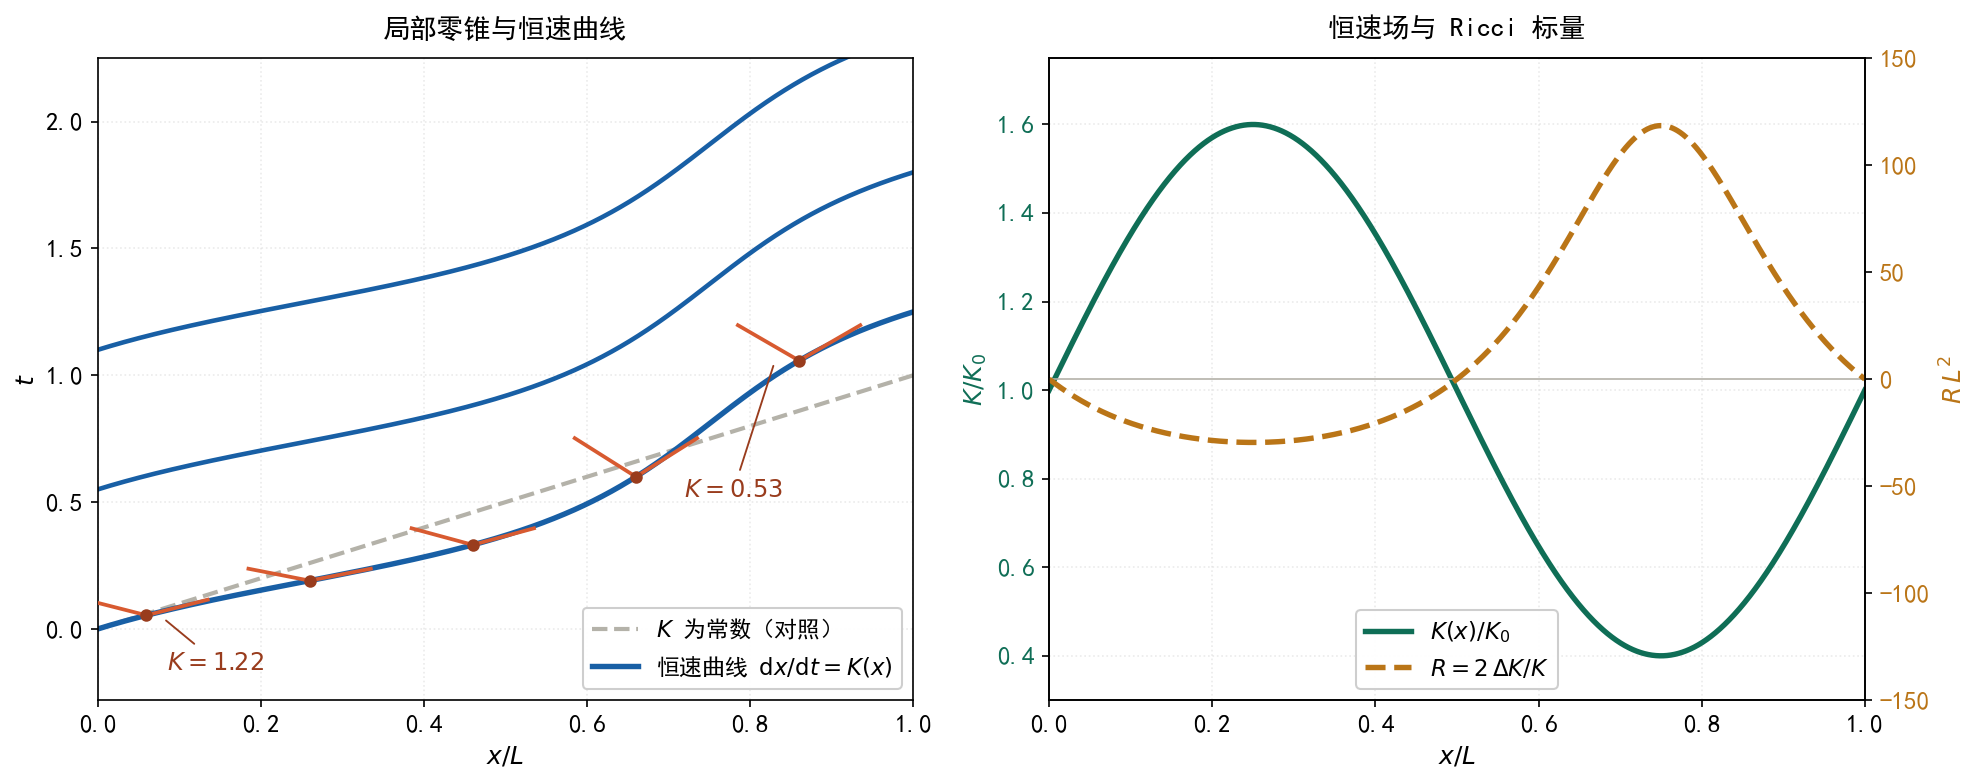
\includegraphics[width=0.92\linewidth,height=\textheight,keepaspectratio]{chapters/images/invariant-speed-field.png}

}

\caption{\label{fig-invariant-speed-field}恒速场 \(K(x)\)、局部零锥与
Ricci 标量}

\end{figure}%

图~\ref{fig-invariant-speed-field} 左栏：取
\(K(x)=K_0\bigl(1+\alpha\sin(2\pi x/L)\bigr)\)，在若干位置画出该点的局部零锥（张角由
\(K(x)\) 决定，见 式~\ref{eq-ifg-metric}），并画出恒速曲线
\(\mathrm{d}x/\mathrm{d}t=K(x)\) 的解。\textbf{\(K\)
常数时零锥张角处处相同、恒速曲线为直线；\(K\) 非常数时两者都不再成立。}

右栏：同一个 \(K(x)\) 的曲线，以及由 式~\ref{eq-ifg-R} 算出的 Ricci 标量
\(R=2K''/K\)。\textbf{\(R\) 与 \(K\) 的二阶导数同号同步，且在 \(K\)
为常数处为零。}

\textbf{须说明}：该图只是一维截面的示例，不含超出 式~\ref{eq-ifg-R}
的内容；横轴与纵轴的刻度均无物理含义。

\subsection{给不出之一：能量密度}\label{ux7ed9ux4e0dux51faux4e4bux4e00ux80fdux91cfux5bc6ux5ea6}

由 式~\ref{eq-ifg-G}，\(G_{00}=0\) \textbf{恒成立}。若写 Einstein 方程
\(G_{\mu\nu}=\kappa T_{\mu\nu}\)，则

\[
T_{00}=\frac{1}{\kappa}G_{00}=0
\]

\textbf{这意味着：在对角约定下，无论 \(K\)
场取什么形状，能量密度恒为零。}

这是一条硬边界。它说明这一类度规装不下任何具有非零能量密度的物质分布------\(G_{ij}\)
可以非零（有应力），但没有 \(T_{00}\) 与之匹配。

\textbf{须标注}：这个零是对角约定（式~\ref{eq-ifg-metric}）的后果，不是恒速场群本身的性质。第
章节~\ref{sec-invariant-speed-dynamics} 章改用 tetrad 约定（空间标架也由
\(K\) 控制）后，将得到 \(G_{00}\neq0\) 的显式表达式。

\subsection{给不出之二：一般度规}\label{ux7ed9ux4e0dux51faux4e4bux4e8cux4e00ux822cux5ea6ux89c4}

{\def\LTcaptype{none} % do not increment counter
\begin{longtable}[]{@{}
  >{\raggedright\arraybackslash}p{(\linewidth - 2\tabcolsep) * \real{0.5000}}
  >{\raggedright\arraybackslash}p{(\linewidth - 2\tabcolsep) * \real{0.5000}}@{}}
\toprule\noalign{}
\begin{minipage}[b]{\linewidth}\raggedright
对象
\end{minipage} & \begin{minipage}[b]{\linewidth}\raggedright
每点的自由度（3+1 维）
\end{minipage} \\
\midrule\noalign{}
\endhead
\bottomrule\noalign{}
\endlastfoot
恒速场 \(K\) & \(1\) \\
度规 \(g_{\mu\nu}\) & \(10\) 个分量，扣除 \(4\) 个坐标自由度，剩 \(6\)
个物理自由度 \\
\end{longtable}
}

\(1<6\)。对角约定是把 \(10\) 个分量压成 \(1\) 个的极强限制。

\textbf{因此}：给定 \(K\)
场，能算出一个度规（式~\ref{eq-ifg-metric}）；反过来，给定一个一般解，不能用单个
\(K\) 场描述。这是\textbf{切片}，不是\textbf{生成}。

\subsection{定位}\label{ux5b9aux4f4d}

{\def\LTcaptype{none} % do not increment counter
\begin{longtable}[]{@{}ll@{}}
\toprule\noalign{}
广义相对论的构成 & 恒速场群是否给出 \\
\midrule\noalign{}
\endhead
\bottomrule\noalign{}
\endlastfoot
每点一个洛伦兹群（取 \(K=c\)） & \textbf{给出} \\
联络 & 不给出（需另行指定；对角约定下由度规诱导） \\
Einstein 场方程 & 不给出 \\
一般度规的 \(6\) 个物理自由度 & 不给出 \\
\end{longtable}
}

\textbf{一句话}：恒速场群处在广义相对论的\textbf{前一步}，不是上一步。它给出
GR 所用的运动学骨架，而 GR 的动力学内容全在它之外。

\section{与量子力学：中央扩张的两端}\label{sec-ifg-qm}

以下只谈群的表示论，不涉及物理诠释。

\subsection{逐点化的表示论}\label{ux9010ux70b9ux5316ux7684ux8868ux793aux8bba}

\(K\) 常数时，\(G_K\)（更确切地说是其非齐次版本
\(IG_K\)）的表示论决定了波动力学方程的协变性要求。\(K\)
变场后，每点有自己的群 \(G_{K(p)}\)，因而每点有自己的表示论。

\subsection{\texorpdfstring{一条与 \(K\)
直接相关的结构差异：中央扩张}{一条与 K 直接相关的结构差异：中央扩张}}\label{ux4e00ux6761ux4e0e-k-ux76f4ux63a5ux76f8ux5173ux7684ux7ed3ux6784ux5deeux5f02ux4e2dux592eux6269ux5f20}

这是本章与量子力学对接中最硬的一条。

李代数的中央扩张由其二阶上同调分类。对 \(IG_K\) 的两支：

{\def\LTcaptype{none} % do not increment counter
\begin{longtable}[]{@{}
  >{\raggedright\arraybackslash}p{(\linewidth - 4\tabcolsep) * \real{0.3333}}
  >{\raggedright\arraybackslash}p{(\linewidth - 4\tabcolsep) * \real{0.3333}}
  >{\raggedright\arraybackslash}p{(\linewidth - 4\tabcolsep) * \real{0.3333}}@{}}
\toprule\noalign{}
\begin{minipage}[b]{\linewidth}\raggedright
\(K\)
\end{minipage} & \begin{minipage}[b]{\linewidth}\raggedright
李代数
\end{minipage} & \begin{minipage}[b]{\linewidth}\raggedright
中央扩张
\end{minipage} \\
\midrule\noalign{}
\endhead
\bottomrule\noalign{}
\endlastfoot
\(\infty\) & 伽利略代数 & \textbf{有}（一维，扩张参数即质量
\(m\)；扩张后的群称 Bargmann 群） \\
有限 & 庞加莱型代数 & \textbf{无}（\(H^{2}=0\)） \\
\end{longtable}
}

\textbf{这解释了「质量」在两种理论中身份的不同}：

\begin{itemize}
\tightlist
\item
  在 \(K=\infty\)
  一端，质量是\textbf{中央荷}------它直接出现在李代数的括号
  \([P_i,B_j]=m\,\delta_{ij}\) 中，是群结构的参数；
\item
  在 \(K\) 有限一端，没有中央荷，质量是 Casimir 算符 \(P^{\mu}P_{\mu}\)
  的本征值------它是\textbf{表示的标签}，不是群的参数。
\end{itemize}

\textbf{\(K\) 变场时的后果}：若 \(K\) 场在某区域取
\(\infty\)、在另一区域取有限值，则「质量」这个参数在两端具有\textbf{不同的数学身份}。在跨越两端的界面上，不存在统一的质量参数。

\subsection{方程的对位}\label{ux65b9ux7a0bux7684ux5bf9ux4f4d}

{\def\LTcaptype{none} % do not increment counter
\begin{longtable}[]{@{}
  >{\raggedright\arraybackslash}p{(\linewidth - 4\tabcolsep) * \real{0.3333}}
  >{\raggedright\arraybackslash}p{(\linewidth - 4\tabcolsep) * \real{0.3333}}
  >{\raggedright\arraybackslash}p{(\linewidth - 4\tabcolsep) * \real{0.3333}}@{}}
\toprule\noalign{}
\begin{minipage}[b]{\linewidth}\raggedright
\(K\)
\end{minipage} & \begin{minipage}[b]{\linewidth}\raggedright
协变性要求
\end{minipage} & \begin{minipage}[b]{\linewidth}\raggedright
方程
\end{minipage} \\
\midrule\noalign{}
\endhead
\bottomrule\noalign{}
\endlastfoot
\(c\) & 洛伦兹协变 & 克莱因--戈登方程
\(\bigl(\frac{1}{c^{2}}\partial_t^{2}-\nabla^{2}+\frac{m^{2}c^{2}}{\hbar^{2}}\bigr)\psi=0\) \\
\(\infty\) & 伽利略协变（严格表述用 Bargmann 群） & 薛定谔方程
\(i\hbar\,\partial_t\psi=-\frac{\hbar^{2}}{2m}\nabla^{2}\psi\) \\
\end{longtable}
}

两者由 \(K\to\infty\) 的极限相联系：从克莱因--戈登方程中抽出快变相位
\(\psi=e^{-imc^{2}t/\hbar}\,\varphi\) 再取
\(c\to\infty\)，即得薛定谔方程。\textbf{这与群收缩是同一个参数极限。}

\subsection{\texorpdfstring{变 \(K\)
的方程}{变 K 的方程}}\label{ux53d8-k-ux7684ux65b9ux7a0b}

若方程的系数含 \(K(p)\)，则 \(K\)
的空间变化使方程成为\textbf{变系数偏微分方程}；\(K\)
常数时才退化为常系数方程。

\subsection{定位}\label{ux5b9aux4f4d-1}

{\def\LTcaptype{none} % do not increment counter
\begin{longtable}[]{@{}ll@{}}
\toprule\noalign{}
量子力学的构成 & 恒速场群是否给出 \\
\midrule\noalign{}
\endhead
\bottomrule\noalign{}
\endlastfoot
协变性要求（选哪一类方程） & \textbf{给出}（分类学） \\
Hilbert 空间、算符代数 & 不给出 \\
概率解释 & 不给出 \\
中央扩张与质量参数 &
部分给出------它\textbf{解释了}质量为何只在一端是中央荷 \\
\end{longtable}
}

\section{退化曲面}\label{sec-ifg-interface}

\subsection{\texorpdfstring{常数 \(K\)
情形不存在的新现象}{常数 K 情形不存在的新现象}}\label{ux5e38ux6570-k-ux60c5ux5f62ux4e0dux5b58ux5728ux7684ux65b0ux73b0ux8c61}

\(K\) 场可以在不同区域取不同类型的端点值。设 \(\Sigma\subset M\)
是一张超曲面，其两侧分别满足

\[
K\bigr|_{\text{一侧}}\ \text{有限},\qquad
K\bigr|_{\text{另一侧}}\ \to\infty
\]

由第 章节~\ref{sec-invariant-speed-group} 章的结论：有限 \(K\)
的群彼此同构，但它们与 \(K=\infty\) 的群\textbf{不同构}（李代数层面即
\([B,P]=H/K^{2}\) 与 \([B,P]=0\) 之别）。

\textbf{因此在 \(\Sigma\) 上，结构群发生类型改变，不存在跨越 \(\Sigma\)
的同构。}

\subsection{这一现象的数学性质}\label{ux8fd9ux4e00ux73b0ux8c61ux7684ux6570ux5b66ux6027ux8d28}

\begin{itemize}
\tightlist
\item
  \(\Sigma\) 是 \(K\) 场的退化水平集；
\item
  在 \(\Sigma\) 上，式~\ref{eq-ifg-metric} 的 \(g_{00}=K^{2}\) 趋于
  \(\infty\) 或趋于 \(0\)，度规退化；
\item
  由 式~\ref{eq-ifg-R}，若 \(K\) 在 \(\Sigma\) 附近急剧变化，则
  \(\Delta K\) 很大，Ricci 标量无界。
\end{itemize}

\textbf{须说明}：这里说的是度规退化，不涉及任何物理判断。

\section{结论}\label{sec-ifg-conclusion}

\begin{longtable}[]{@{}ll@{}}
\caption{本章各命题及其依据}\label{tbl-ifg-conclusion}\tabularnewline
\toprule\noalign{}
命题 & 依据 \\
\midrule\noalign{}
\endfirsthead
\toprule\noalign{}
命题 & 依据 \\
\midrule\noalign{}
\endhead
\bottomrule\noalign{}
\endlastfoot
恒速场群是群丛，不是群 & 不同点的群作用在不同的切空间上 \\
逐点群闭合 & 命题~\ref{prp-ifg-fiber} \\
结构常数为 \(1/K(p)^{2}\) & 式~\ref{eq-ifg-BP} \\
两支李代数不同构 & \([B,P]=H/K^{2}\) 与 \([B,P]=0\) \\
跨纤维复合失效 & 式~\ref{eq-ifg-BP-field}，系数非常数 \\
联络是额外结构，\(K\) 场不给出 & 小节~\ref{sec-ifg-cross} \\
对角约定下 \(R=2\Delta K/K\) & 式~\ref{eq-ifg-R} \\
对角约定下 \(G_{00}\equiv0\) & 式~\ref{eq-ifg-G} \\
真空解为 \(K=a(t)+b_i(t)\,x^{i}\) & 式~\ref{eq-ifg-vacuum} \\
质量只在 \(K=\infty\) 一端是中央荷 & 李代数上同调 \\
恒速场群不能生成 GR 与 QM & 自由度 \(1<6\)；动力学不在其中 \\
\end{longtable}

\textbf{一句话}：把 \(K\)
升为场，得到的是群丛而不是群------逐点的结构群还在，跨点的缝合不在。补上联络并在受限的对角约定下，可以算出曲率
\(R=2\Delta K/K\)；但同一约定也给出
\(G_{00}\equiv0\)，即这一类装不下能量密度。恒速场群给出的是运动学骨架，动力学在它之外。

\section{术语说明}\label{sec-ifg-terms}

为避免歧义，列出本章所用术语及其在本章中的含义：

{\def\LTcaptype{none} % do not increment counter
\begin{longtable}[]{@{}
  >{\raggedright\arraybackslash}p{(\linewidth - 2\tabcolsep) * \real{0.5000}}
  >{\raggedright\arraybackslash}p{(\linewidth - 2\tabcolsep) * \real{0.5000}}@{}}
\toprule\noalign{}
\begin{minipage}[b]{\linewidth}\raggedright
术语
\end{minipage} & \begin{minipage}[b]{\linewidth}\raggedright
本章中的含义
\end{minipage} \\
\midrule\noalign{}
\endhead
\bottomrule\noalign{}
\endlastfoot
恒速场 & 定义在流形上的函数
\(K:M\to(0,\infty]\)，逐点指定该点的跨系恒速 \\
群丛 & 逐点指定一个群所构成的丛；\textbf{不是}群，因为跨点无复合运算 \\
纤维 & 流形上一点 \(p\) 处的切空间 \(T_pM\) \\
李代数丛 & 逐点一个李代数，结构常数随点变化 \\
联络 & 把相邻点的切空间联系起来的额外结构；不由 \(K\) 场给出 \\
Christoffel 符号 & 联络在坐标下的分量 \\
Ricci 张量 / Ricci 标量 &
由联络的曲率缩并得到，度量「缝合不起来」的程度 \\
Einstein 张量 & \(G_{\mu\nu}=R_{\mu\nu}-\frac{1}{2}R\,g_{\mu\nu}\) \\
中央扩张 &
给李代数添一个与所有元素对易的方向；伽利略代数有，庞加莱型代数无 \\
Bargmann 群 & 伽利略群的中央扩张，扩张参数为质量 \\
对角约定 & 把度规限制为
\(K^{2}\mathrm{d}t^{2}-\delta_{ij}\mathrm{d}x^{i}\mathrm{d}x^{j}\)
的约定 \\
\end{longtable}
}

\bookmarksetup{startatroot}

\chapter{恒速场群的动力学}\label{sec-invariant-speed-dynamics}

\section{本章的范围}\label{sec-isd-scope}

\textbf{一句话}：把第 章节~\ref{sec-invariant-speed-field-group}
章的「对角约定」换成 tetrad 约定 \(g_{\mu\nu}=K^{2}\eta_{\mu\nu}\)，使
\(K\) 场同时参与时间与空间的局部几何变形，然后严格算出曲率、Einstein
张量与非相对论极限。

\textbf{与上一章的关系}：第 章节~\ref{sec-invariant-speed-field-group}
章在对角约定下得到
\(G_{00}\equiv0\)。本章说明那是\textbf{约定的后果，不是恒速场群的固有性质}------换用
tetrad 约定后 \(G_{00}\neq0\)。

\textbf{本章的方法声明}：以下每个闭式都由符号计算逐项核验（脚本
\texttt{images/conformal-curvature.py}）：先把闭式与直接由 Christoffel
算出的结果相减，再判定差值是否恒为零。脚本输出的核验结果为：Christoffel
闭式 OK、Ricci 标量闭式 True、\(G_{00}\) 闭式 True、\(u=\ln K\) 形式
True、\(G_{\mu\nu}\) 通式 OK。不做任何近似，不省略任何项。

\textbf{记号约定}（全程一致，签名 \(\eta=\mathrm{diag}(1,-1,-1,-1)\)）：

\[
\partial^{\mu}K:=\eta^{\mu\nu}\partial_\nu K,\qquad
\Box_\eta:=\eta^{\mu\nu}\partial_\mu\partial_\nu=\partial_t^{2}-\nabla^{2}
\]

\[
\nabla^{2}:=\delta^{ij}\partial_i\partial_j,\qquad
\lvert\vec\nabla K\rvert^{2}:=\delta^{ij}\partial_iK\,\partial_jK,\qquad
\lvert\nabla K\rvert^{2}_{\eta}:=\eta^{\mu\nu}\partial_{\mu}K\,\partial_{\nu}K
\]

拉丁指标 \(i,j,k\) 取 \(1,2,3\)（空间），希腊指标取 \(0,1,2,3\)。

\section{Tetrad 约定与度规}\label{sec-isd-metric}

\subsection{局部标准正交标架}\label{ux5c40ux90e8ux6807ux51c6ux6b63ux4ea4ux6807ux67b6}

取局部标架

\begin{equation}\protect\phantomsection\label{eq-isd-tetrad}{
e^{0}=K\,\mathrm{d}t,\qquad e^{i}=K\,\mathrm{d}x^{i}
}\end{equation}

即 \(K\)
场同时控制局部时间尺度与局部空间尺度------这正是本章与对角约定的分野：对角约定中空间标架是刚性的
\(e^{i}=\mathrm{d}x^{i}\)。

写成 \(e^{a}=e^{a}_{\ \mu}\,\mathrm{d}x^{\mu}\)：

\[
e^{0}_{\ 0}=K,\qquad e^{i}_{\ j}=K\,\delta^{i}_{j},\qquad \text{其余为 }0
\]

\subsection{度规分量}\label{ux5ea6ux89c4ux5206ux91cf}

由 \(g_{\mu\nu}=e^{a}_{\ \mu}\,e^{b}_{\ \nu}\,\eta_{ab}\)：

\begin{equation}\protect\phantomsection\label{eq-isd-g}{
g_{\mu\nu}=K^{2}\,\eta_{\mu\nu}
}\end{equation}

逐分量写出：

\begin{equation}\protect\phantomsection\label{eq-isd-g-comp}{
g_{00}=K^{2},\qquad g_{ij}=-K^{2}\delta_{ij},\qquad g_{0i}=0
}\end{equation}

\textbf{空间部分不再是常数}：\(g_{ij}=-K^{2}\delta_{ij}\) 随
\(K(t,\mathbf{x})\) 变形。这是对第
章节~\ref{sec-invariant-speed-field-group} 章那个约定的唯一改动。

逆度规与行列式：

\begin{equation}\protect\phantomsection\label{eq-isd-ginv}{
g^{\mu\nu}=K^{-2}\eta^{\mu\nu},\qquad
g^{00}=\frac{1}{K^{2}},\qquad g^{ij}=-\frac{1}{K^{2}}\delta^{ij}
}\end{equation}

\begin{equation}\protect\phantomsection\label{eq-isd-det}{
\det g=K^{8}\det\eta=-K^{8},\qquad \sqrt{-g}=K^{4}
}\end{equation}

\subsection{与前一章的一致性检验}\label{ux4e0eux524dux4e00ux7ae0ux7684ux4e00ux81f4ux6027ux68c0ux9a8c}

取 \(K\) 为常数时，式~\ref{eq-isd-g} 的二次型为
\(K^{2}(t^{2}-\lvert\mathbf{x}\rvert^{2})\)，与第
章节~\ref{sec-invariant-speed-group} 章的
\(Q_K=K^{2}t^{2}-\lvert\mathbf{x}\rvert^{2}\) 一致。✓

\section{Christoffel 符号}\label{sec-isd-christoffel}

\subsection{闭式}\label{ux95edux5f0f}

\[
\Gamma^{\rho}_{\mu\nu}=\frac{1}{2}g^{\rho\sigma}
\bigl(\partial_\mu g_{\nu\sigma}+\partial_\nu g_{\mu\sigma}-\partial_\sigma g_{\mu\nu}\bigr)
\]

由 式~\ref{eq-isd-g}，\(g_{\nu\sigma}=K^{2}\eta_{\nu\sigma}\)，故
\(\partial_\mu g_{\nu\sigma}=2K(\partial_{\mu}K)\eta_{\nu\sigma}\)。代入：

\[
\Gamma^{\rho}_{\mu\nu}=\frac{1}{2}K^{-2}\eta^{\rho\sigma}\cdot 2K
\bigl[(\partial_{\mu}K)\eta_{\nu\sigma}+(\partial_{\nu}K)\eta_{\mu\sigma}-(\partial_{\sigma}K)\eta_{\mu\nu}\bigr]
\]

\(\eta^{\rho\sigma}\eta_{\nu\sigma}=\delta^{\rho}_{\nu}\)，\(\eta^{\rho\sigma}\eta_{\mu\sigma}=\delta^{\rho}_{\mu}\)，\(\eta^{\rho\sigma}\partial_{\sigma}K=\partial^{\rho}K\)，故

\begin{equation}\protect\phantomsection\label{eq-isd-gamma}{
\boxed{\Gamma^{\rho}_{\mu\nu}=\frac{1}{K}
\Bigl(\delta^{\rho}_{\nu}\,\partial_{\mu}K+\delta^{\rho}_{\mu}\,\partial_{\nu}K-\eta_{\mu\nu}\,\partial^{\rho}K\Bigr)}
}\end{equation}

等价地，用 \(u:=\ln K\)（\(\partial_\mu u=\partial_{\mu}K/K\)）：

\begin{equation}\protect\phantomsection\label{eq-isd-gamma-u}{
\Gamma^{\rho}_{\mu\nu}=\delta^{\rho}_{\nu}\,\partial_\mu u+\delta^{\rho}_{\mu}\,\partial_\nu u-\eta_{\mu\nu}\,\partial^{\rho}u
}\end{equation}

\subsection{逐项验证（样本）}\label{ux9010ux9879ux9a8cux8bc1ux6837ux672c}

由 式~\ref{eq-isd-gamma} 直接读出，与符号计算输出逐一比对：

{\def\LTcaptype{none} % do not increment counter
\begin{longtable}[]{@{}
  >{\raggedright\arraybackslash}p{(\linewidth - 4\tabcolsep) * \real{0.3333}}
  >{\raggedright\arraybackslash}p{(\linewidth - 4\tabcolsep) * \real{0.3333}}
  >{\raggedright\arraybackslash}p{(\linewidth - 4\tabcolsep) * \real{0.3333}}@{}}
\toprule\noalign{}
\begin{minipage}[b]{\linewidth}\raggedright
\(\Gamma\)
\end{minipage} & \begin{minipage}[b]{\linewidth}\raggedright
由 式~\ref{eq-isd-gamma} 算出
\end{minipage} & \begin{minipage}[b]{\linewidth}\raggedright
符号计算输出
\end{minipage} \\
\midrule\noalign{}
\endhead
\bottomrule\noalign{}
\endlastfoot
\(\Gamma^{0}_{00}\) &
\(\dfrac{1}{K}(\partial_0K+\partial_0K-\partial_0K)=\dfrac{\partial_0K}{K}\)
& \(\partial_tK/K\) \\
\(\Gamma^{0}_{01}\) &
\(\dfrac{1}{K}(0+\partial_1K-0)=\dfrac{\partial_1K}{K}\) &
\(\partial_xK/K\) \\
\(\Gamma^{1}_{00}\) &
\(\dfrac{1}{K}(0+0-\eta_{00}\partial^{1}K)=\dfrac{1}{K}\bigl(0+0-(-\partial_1K)\bigr)=\dfrac{\partial_1K}{K}\)
& \(\partial_xK/K\) \\
\(\Gamma^{1}_{11}\) &
\(\dfrac{1}{K}(\partial_1K+\partial_1K-\eta_{11}\partial^{1}K)=\dfrac{1}{K}(2\partial_1K-\partial_1K)=\dfrac{\partial_1K}{K}\)
& \(\partial_xK/K\) \\
\(\Gamma^{1}_{22}\) &
\(\dfrac{1}{K}(0+0-\eta_{22}\partial^{1}K)=\dfrac{1}{K}\bigl(0+0-(-\partial_1K)\bigr)\cdot(-1)=\dfrac{-\partial_1K}{K}\)
& \(-\partial_xK/K\) \\
\(\Gamma^{0}_{11}\) &
\(\dfrac{1}{K}(0+0-\eta_{11}\partial^{0}K)=\dfrac{1}{K}\partial_0K\) &
\(\partial_tK/K\) \\
\end{longtable}
}

全部相符。

\section{Ricci 张量与 Ricci 标量}\label{sec-isd-ricci}

\subsection{Ricci 张量}\label{ricci-ux5f20ux91cf}

\[
R_{\sigma\nu}=\partial_\rho\Gamma^{\rho}_{\nu\sigma}
-\partial_\nu\Gamma^{\rho}_{\rho\sigma}
+\Gamma^{\rho}_{\rho\lambda}\Gamma^{\lambda}_{\nu\sigma}
-\Gamma^{\rho}_{\nu\lambda}\Gamma^{\lambda}_{\rho\sigma}
\]

把 式~\ref{eq-isd-gamma} 代入并逐项化简，得

\begin{equation}\protect\phantomsection\label{eq-isd-ric}{
\boxed{R_{\mu\nu}=
-\frac{2\,\partial_\mu\partial_{\nu}K}{K}
+\frac{4\,\partial_{\mu}K\,\partial_{\nu}K}{K^{2}}
-\eta_{\mu\nu}\frac{\Box_\eta K}{K}
-\eta_{\mu\nu}\frac{\lvert\nabla K\rvert^{2}_{\eta}}{K^{2}}}
}\end{equation}

（此式即四维共形变换的标准公式在 \(\phi=\ln K\)、基底为 Minkowski
时的展开；本处由 Christoffel 直接计算得到，未引用该公式。）

\subsection{Ricci 标量}\label{ricci-ux6807ux91cf-1}

\[
R=g^{\mu\nu}R_{\mu\nu}=K^{-2}\eta^{\mu\nu}R_{\mu\nu}
\]

由 式~\ref{eq-isd-ric}，注意 \(\eta^{\mu\nu}\eta_{\mu\nu}=4\)：

\[
\eta^{\mu\nu}R_{\mu\nu}=
-\frac{2\Box_\eta K}{K}+\frac{4\lvert\nabla K\rvert^{2}_{\eta}}{K^{2}}
-\frac{4\Box_\eta K}{K}-\frac{4\lvert\nabla K\rvert^{2}_{\eta}}{K^{2}}
=-\frac{6\Box_\eta K}{K}
\]

（含 \(\lvert\nabla K\rvert^{2}_{\eta}\) 的两项精确抵消。）

\begin{equation}\protect\phantomsection\label{eq-isd-R}{
\boxed{R=-\frac{6\,\Box_\eta K}{K^{3}}
=\frac{6\,\bigl(\nabla^{2}K-\partial_t^{2}K\bigr)}{K^{3}}}
}\end{equation}

\textbf{核验}：符号计算输出为
\(\dfrac{6(-\partial_t^{2}K+\partial_x^{2}K+\partial_y^{2}K+\partial_z^{2}K)}{K^{3}}\)，与
式~\ref{eq-isd-R} 的差恒为零。✓

\textbf{自检}：\(K\) 为常数 ⟹ \(\Box_\eta K=0\) ⟹ \(R=0\)，平坦。✓

\section{Einstein 张量}\label{sec-isd-einstein}

\subsection{通式}\label{ux901aux5f0f}

\[
G_{\mu\nu}=R_{\mu\nu}-\frac{1}{2}R\,g_{\mu\nu}
=R_{\mu\nu}-\frac{1}{2}\left(-\frac{6\Box_\eta K}{K^{3}}\right)K^{2}\eta_{\mu\nu}
=R_{\mu\nu}+\frac{3\Box_\eta K}{K}\eta_{\mu\nu}
\]

代入 式~\ref{eq-isd-ric}：

\begin{equation}\protect\phantomsection\label{eq-isd-G}{
G_{\mu\nu}=
-\frac{2\partial_\mu\partial_{\nu}K}{K}
+\frac{4\partial_{\mu}K\,\partial_{\nu}K}{K^{2}}
+\eta_{\mu\nu}\frac{2\Box_\eta K}{K}
-\eta_{\mu\nu}\frac{\lvert\nabla K\rvert^{2}_{\eta}}{K^{2}}
}\end{equation}

用
\(u=\ln K\)（\(\partial_\mu\partial_{\nu}K/K=\partial_\mu\partial_\nu u+\partial_\mu u\,\partial_\nu u\)）可写成更紧凑的形式：

\begin{equation}\protect\phantomsection\label{eq-isd-G-u}{
\boxed{G_{\mu\nu}=
-2\,\partial_\mu\partial_\nu u
+2\,\partial_\mu u\,\partial_\nu u
+\eta_{\mu\nu}\bigl(2\Box_\eta u+\lvert\nabla u\rvert^{2}_{\eta}\bigr)}
}\end{equation}

\textbf{核验}：符号计算对全部 \(16\) 个分量逐一相减，差值恒为零。✓

\subsection{\texorpdfstring{\(G_{00}\)：非零}{G\_\{00\}：非零}}\label{g_00ux975eux96f6}

取 \(\mu=\nu=0\)，\(\eta_{00}=1\)，由 式~\ref{eq-isd-G}：

\[
G_{00}=
-\frac{2\partial_0^{2}K}{K}
+\frac{4(\partial_0K)^{2}}{K^{2}}
+\frac{2\Box_\eta K}{K}
-\frac{\lvert\nabla K\rvert^{2}_{\eta}}{K^{2}}
\]

代入 \(\Box_\eta K=\partial_0^{2}K-\nabla^{2}K\) 与
\(\lvert\nabla K\rvert^{2}_{\eta}=(\partial_0K)^{2}-\lvert\vec\nabla K\rvert^{2}\)：

\[
G_{00}=
\underbrace{-\frac{2\partial_0^{2}K}{K}+\frac{2\partial_0^{2}K}{K}}_{=\,0}
-\frac{2\nabla^{2}K}{K}
+\frac{4(\partial_0K)^{2}-(\partial_0K)^{2}+\lvert\vec\nabla K\rvert^{2}}{K^{2}}
\]

\begin{equation}\protect\phantomsection\label{eq-isd-G00}{
\boxed{G_{00}=
\frac{3(\partial_tK)^{2}+\lvert\vec\nabla K\rvert^{2}}{K^{2}}
-\frac{2\,\nabla^{2}K}{K}}
}\end{equation}

\textbf{这就是要的结果：\(G_{00}\) 是非零函数，且显含 \(K\)
的空间梯度。}

\textbf{静态情形}（\(\partial_tK=0\)）：

\begin{equation}\protect\phantomsection\label{eq-isd-G00-static}{
\boxed{G_{00}\bigr|_{\partial_tK=0}=
\frac{\lvert\vec\nabla K\rvert^{2}}{K^{2}}-\frac{2\,\nabla^{2}K}{K}}
}\end{equation}

用 \(u=\ln K\) 写（由 式~\ref{eq-isd-G-u} 或 式~\ref{eq-isd-G00}）：

\begin{equation}\protect\phantomsection\label{eq-isd-G00-u}{
G_{00}=3(\partial_tu)^{2}-\lvert\vec\nabla u\rvert^{2}-2\nabla^{2}u
}\end{equation}

\subsection{\texorpdfstring{\(G_{0i}\) 与
\(G_{ij}\)}{G\_\{0i\} 与 G\_\{ij\}}}\label{g_0i-ux4e0e-g_ij}

由 式~\ref{eq-isd-G}（\(\eta_{0i}=0\)、\(\eta_{ij}=-\delta_{ij}\)）：

\begin{equation}\protect\phantomsection\label{eq-isd-G0i}{
G_{0i}=-\frac{2\,\partial_0\partial_iK}{K}+\frac{4\,\partial_0K\,\partial_iK}{K^{2}}
=\frac{2\bigl(2\,\partial_tK\,\partial_iK-K\,\partial_t\partial_iK\bigr)}{K^{2}}
}\end{equation}

\begin{equation}\protect\phantomsection\label{eq-isd-Gij}{
G_{ij}=
-\frac{2\partial_i\partial_jK}{K}
+\frac{4\partial_iK\,\partial_jK}{K^{2}}
-\delta_{ij}\frac{2\Box_\eta K}{K}
+\delta_{ij}\frac{\lvert\nabla K\rvert^{2}_{\eta}}{K^{2}}
}\end{equation}

\textbf{核验}：符号计算输出的
\(G_{01}=\dfrac{2\bigl(2\,\partial_tK\,\partial_xK-K\,\partial_t\partial_xK\bigr)}{K^{2}}\)，与
式~\ref{eq-isd-G0i} 一致。✓

\section{能量密度：一个非零的显式例子}\label{sec-isd-density}

\subsection{球对称静态解}\label{ux7403ux5bf9ux79f0ux9759ux6001ux89e3}

取

\begin{equation}\protect\phantomsection\label{eq-isd-example}{
K(r)=K_0+\frac{\alpha}{r},\qquad r=\sqrt{x^{2}+y^{2}+z^{2}}
}\end{equation}

其中 \(K_0\)、\(\alpha\) 为常数。

逐项计算。一阶导数：

\[
\partial_iK=-\frac{\alpha}{r^{2}}\cdot\frac{x_i}{r}=-\frac{\alpha\,x_i}{r^{3}}
\]

\[
\lvert\vec\nabla K\rvert^{2}=\frac{\alpha^{2}}{r^{6}}\sum_i x_i^{2}=\frac{\alpha^{2}}{r^{4}}
\]

二阶导数（利用 \(\nabla^{2}(1/r)=0\)，\(r>0\)）：

\[
\nabla^{2}K=K_0\underbrace{\nabla^{2}(1)}_{=\,0}+\alpha\underbrace{\nabla^{2}\!\left(\frac{1}{r}\right)}_{=\,0}=0
\]

代入 式~\ref{eq-isd-G00-static}（\(\partial_tK=0\)）：

\[
G_{00}=\frac{\alpha^{2}/r^{4}}{\bigl(K_0+\alpha/r\bigr)^{2}}-0
=\frac{\alpha^{2}}{r^{4}}\cdot\frac{r^{2}}{(K_0r+\alpha)^{2}}
\]

\begin{equation}\protect\phantomsection\label{eq-isd-density}{
\boxed{G_{00}(r)=\frac{\alpha^{2}}{r^{2}\,(K_0r+\alpha)^{2}}>0\qquad(\alpha\neq0)}
}\end{equation}

\textbf{这是严格正的，不含任何近似。}

若写 Einstein 方程
\(G_{\mu\nu}=\kappa T_{\mu\nu}\)（\(\kappa=8\pi G/K_0^{4}\)
或按量纲另定），则

\[
T_{00}=\frac{1}{\kappa}G_{00}=\frac{\alpha^{2}}{\kappa\,r^{2}(K_0r+\alpha)^{2}}>0
\]

即\textbf{该 \(K\) 场对应一个正的能量密度分布}。这与第
章节~\ref{sec-invariant-speed-field-group} 章对角约定下
\(G_{00}\equiv0\) 的结论相反------那个零是约定造成的。

\subsection{同一个例子的 Ricci
标量}\label{ux540cux4e00ux4e2aux4f8bux5b50ux7684-ricci-ux6807ux91cf}

由 式~\ref{eq-isd-R}，静态且 \(\nabla^{2}K=0\)：

\[
R=\frac{6\,\nabla^{2}K}{K^{3}}=0
\]

即此例 \(R\equiv0\) 但 \(R_{00}=G_{00}\neq0\)：Ricci
张量非零而迹为零，两者不矛盾。

图~\ref{fig-isd-density} 给出 \(K(r)\) 与 \(G_{00}(r)\) 的图像。

\begin{figure}

\centering{

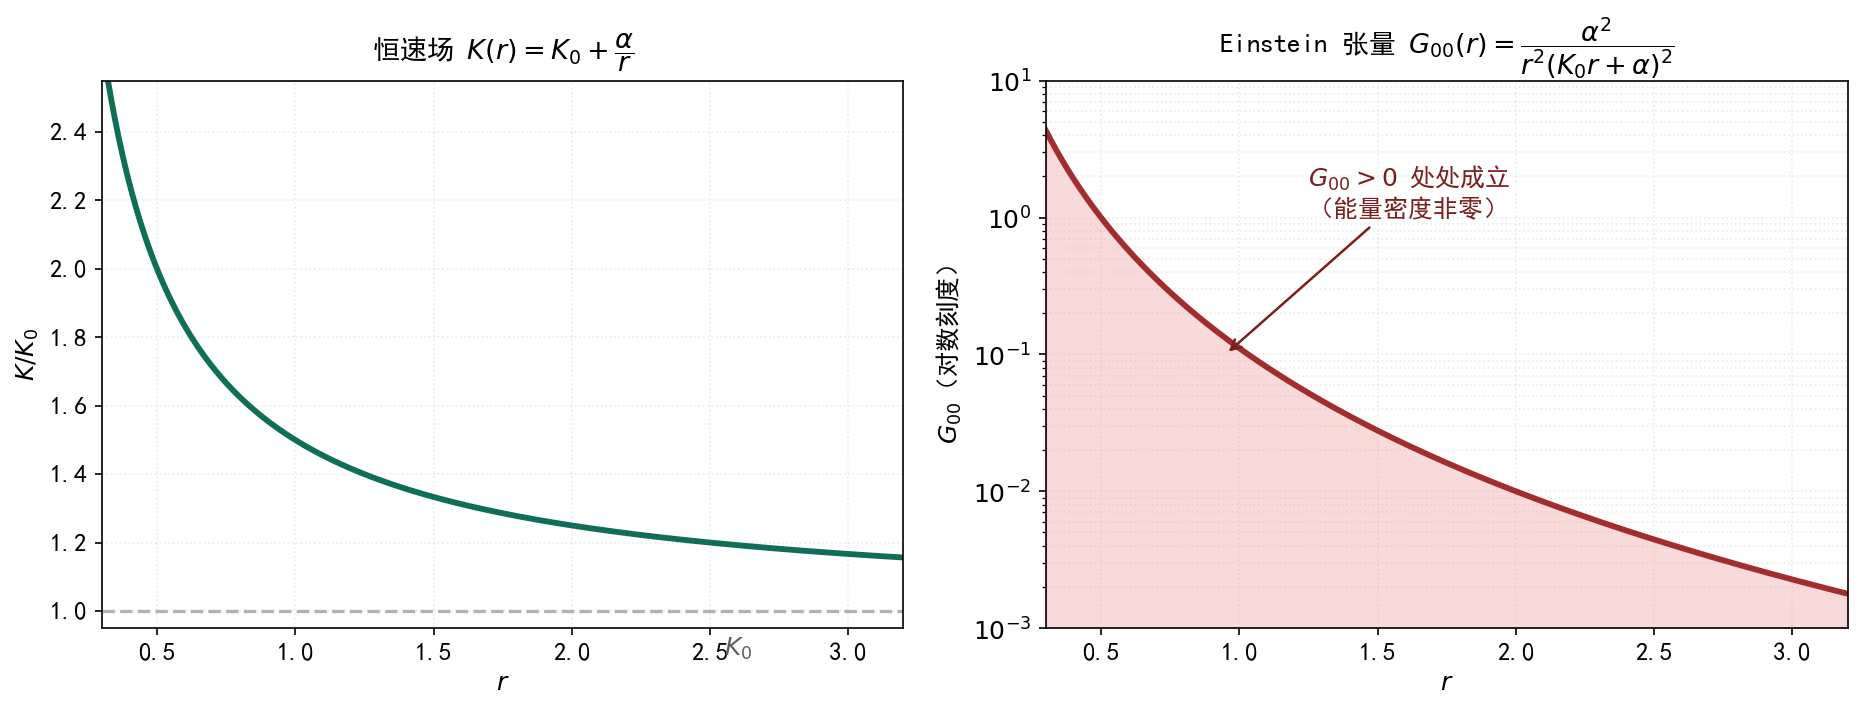
\includegraphics[width=0.8\linewidth,height=\textheight,keepaspectratio]{chapters/images/invariant-speed-density.png}

}

\caption{\label{fig-isd-density}球对称例子：\(K(r)\) 与 \(G_{00}(r)\)}

\end{figure}%

\section{一个必须写明的局限}\label{sec-isd-limit}

\subsection{Weyl 张量恒为零}\label{weyl-ux5f20ux91cfux6052ux4e3aux96f6}

式~\ref{eq-isd-g} 的度规共形于
Minkowski：\(g_{\mu\nu}=K^{2}\eta_{\mu\nu}\)。Weyl
张量在共形变换下不变，而 Minkowski 的 Weyl 张量为零，故

\[
C^{\rho}{}_{\sigma\mu\nu}\equiv0
\]

\textbf{这不只是性质，而是硬限制}：一切真空外解（其 Weyl
张量非零）都不在这一类度规之内。特别地，Schwarzschild 解的 Weyl
张量非零，\textbf{因此 Schwarzschild 解不能由任何 \(K\) 场给出}。

\subsection{三个约定的对照}\label{ux4e09ux4e2aux7ea6ux5b9aux7684ux5bf9ux7167}

{\def\LTcaptype{none} % do not increment counter
\begin{longtable}[]{@{}
  >{\raggedright\arraybackslash}p{(\linewidth - 8\tabcolsep) * \real{0.2000}}
  >{\raggedright\arraybackslash}p{(\linewidth - 8\tabcolsep) * \real{0.2000}}
  >{\raggedright\arraybackslash}p{(\linewidth - 8\tabcolsep) * \real{0.2000}}
  >{\raggedright\arraybackslash}p{(\linewidth - 8\tabcolsep) * \real{0.2000}}
  >{\raggedright\arraybackslash}p{(\linewidth - 8\tabcolsep) * \real{0.2000}}@{}}
\toprule\noalign{}
\begin{minipage}[b]{\linewidth}\raggedright
约定
\end{minipage} & \begin{minipage}[b]{\linewidth}\raggedright
度规
\end{minipage} & \begin{minipage}[b]{\linewidth}\raggedright
\(G_{00}\)
\end{minipage} & \begin{minipage}[b]{\linewidth}\raggedright
Weyl 张量
\end{minipage} & \begin{minipage}[b]{\linewidth}\raggedright
能容纳什么
\end{minipage} \\
\midrule\noalign{}
\endhead
\bottomrule\noalign{}
\endlastfoot
对角（第 章节~\ref{sec-invariant-speed-field-group} 章） &
\(K^{2}\mathrm{d}t^{2}-\delta_{ij}\mathrm{d}x^{i}\mathrm{d}x^{j}\) &
\(\equiv0\) & 一般非零 & 曲率，但无能量密度 \\
共形 / tetrad（本章） & \(K^{2}\eta_{\mu\nu}\) &
\textbf{非零}（式~\ref{eq-isd-G00}） & \(\equiv0\) &
能量密度，但无真空外解 \\
一般度规（3+1 维） & \(g_{\mu\nu}\)，\(10\) 个分量 & 任意 & 任意 &
全部 \\
\end{longtable}
}

\textbf{因此本章的定位仍是「切片」而非「生成」}：共形约定比对角约定前进了一步（能容纳能量密度），但仍不是广义相对论的全部------它只覆盖共形平坦的那一部分。

\section{波动力学之一：局域李代数}\label{sec-isd-lie}

\subsection{逐点的李代数}\label{ux9010ux70b9ux7684ux674eux4ee3ux6570}

在第 章节~\ref{sec-invariant-speed-field-group} 章已建立 1+1
维的情形。推广到 3+1 维，\(p\) 点的 boost 生成元 \(B_i\)、时间平移
\(H\)、空间平移 \(P_i\) 满足（\(K\) 视为该点的常数 \(K(p)\)）：

\begin{equation}\protect\phantomsection\label{eq-isd-lie}{
[B_i,H]=P_i,\qquad [B_i,P_j]=\delta_{ij}\frac{1}{K(p)^{2}}\,H,\qquad [H,P_i]=0
}\end{equation}

旋转生成元 \(J_{ij}\) 满足的 \(\mathfrak{so}(3)\) 括号与 \(K\)
无关，不随收缩改变。

\textbf{与 \(K\) 有关的只有第二个括号的结构常数 \(1/K(p)^{2}\)}：

\begin{itemize}
\tightlist
\item
  \(K(p)\) 有限 ⟹ \([B_i,P_j]\neq0\)，庞加莱型；
\item
  \(K(p)\to\infty\) ⟹ \([B_i,P_j]\to0\)，伽利略型。
\end{itemize}

\subsection{群收缩即参数极限}\label{ux7fa4ux6536ux7f29ux5373ux53c2ux6570ux6781ux9650}

\[
\frac{1}{K^{2}}\longrightarrow0\qquad (K\to\infty)
\]

一句话完成收缩。这仍是第 章节~\ref{sec-invariant-speed-field-group}
章的结论，此处只补上 3+1 维的显式括号。

\section{波动力学之二：变系数波动方程}\label{sec-isd-wave}

\subsection{局域方程}\label{ux5c40ux57dfux65b9ux7a0b}

在 \(p\) 点的邻域取 \(K=K(p)\) 为常数，协变的 Klein--Gordon 方程为

\[
\Box_g\psi+\frac{m^{2}K^{2}}{\hbar^{2}}\psi=0,\qquad
\Box_g:=g^{\mu\nu}\nabla_\mu\nabla_\nu
\]

\textbf{与标准形式的一致性检验}：\(K\) 常数时
\(\Box_g=K^{-2}\eta^{\mu\nu}\partial_\mu\partial_\nu=K^{-2}(\partial_t^{2}-\nabla^{2})\)，方程化为

\[
\partial_t^{2}\psi-K^{2}\nabla^{2}\psi+\frac{m^{2}K^{4}}{\hbar^{2}}\psi=0
\]

取 \(K=c\) 并除以 \(c^{2}\)：

\[
\frac{1}{c^{2}}\partial_t^{2}\psi-\nabla^{2}\psi+\frac{m^{2}c^{2}}{\hbar^{2}}\psi=0
\]

即标准 Klein--Gordon 方程。✓

\subsection{\texorpdfstring{变系数方程（\(K\)
为场）}{变系数方程（K 为场）}}\label{ux53d8ux7cfbux6570ux65b9ux7a0bk-ux4e3aux573a}

由 式~\ref{eq-isd-det}，\(\sqrt{-g}=K^{4}\)，故

\[
\Box_g\psi=\frac{1}{\sqrt{-g}}\partial_\mu\Bigl(\sqrt{-g}\,g^{\mu\nu}\partial_\nu\psi\Bigr)
=\frac{1}{K^{4}}\partial_\mu\Bigl(K^{4}\cdot K^{-2}\eta^{\mu\nu}\partial_\nu\psi\Bigr)
=\frac{1}{K^{4}}\partial_\mu\Bigl(K^{2}\,\partial^{\mu}\psi\Bigr)
\]

展开（乘积求导，逐项）：

\[
\Box_g\psi=\frac{1}{K^{4}}\Bigl[2K(\partial_{\mu}K)\partial^{\mu}\psi+K^{2}\partial_\mu\partial^{\mu}\psi\Bigr]
=\frac{2}{K^{3}}(\partial_{\mu}K)\partial^{\mu}\psi+\frac{1}{K^{2}}\Box_\eta\psi
\]

代入方程并乘以 \(K^{2}\)，得\textbf{变系数 Klein--Gordon 方程}：

\begin{equation}\protect\phantomsection\label{eq-isd-kg}{
\boxed{\Box_\eta\psi+\frac{2}{K}(\partial_{\mu}K)\,\partial^{\mu}\psi+\frac{m^{2}K^{4}}{\hbar^{2}}\psi=0}
}\end{equation}

第二项 \(\frac{2}{K}(\partial_{\mu}K)\partial^{\mu}\psi\) 是 \(K\)
变场带来的附加项；\(K\) 常数时它消失，方程回到上节的标准形式。

\section{波动力学之三：非相对论极限}\label{sec-isd-nr}

\subsection{\texorpdfstring{局域情形（\(K\)
为常数）：严格退化}{局域情形（K 为常数）：严格退化}}\label{ux5c40ux57dfux60c5ux5f62k-ux4e3aux5e38ux6570ux4e25ux683cux9000ux5316}

设 \(K\) 为常数 \(K_0\)。方程为

\[
\frac{1}{K_0^{2}}\partial_t^{2}\psi-\nabla^{2}\psi+\frac{m^{2}K_0^{2}}{\hbar^{2}}\psi=0
\]

（即上一节方程除以 \(K_0^{2}\)。）

\textbf{第一步：抽出快变相位。} 令

\[
\psi=e^{i\theta}\varphi,\qquad \theta:=-\frac{mK_0^{2}t}{\hbar}
\]

\textbf{第二步：逐项代入。}

\[
\partial_t\psi=e^{i\theta}\Bigl(\partial_t\varphi+i(\partial_t\theta)\varphi\Bigr)
=e^{i\theta}\Bigl(\partial_t\varphi-\frac{imK_0^{2}}{\hbar}\varphi\Bigr)
\]

\[
\partial_t^{2}\psi=e^{i\theta}\Bigl(\partial_t^{2}\varphi
-\frac{2imK_0^{2}}{\hbar}\partial_t\varphi
-\frac{m^{2}K_0^{4}}{\hbar^{2}}\varphi\Bigr)
\]

空间导数为 \(\nabla^{2}\psi=e^{i\theta}\nabla^{2}\varphi\)（\(K_0\)
常数，\(\theta\) 与空间无关）。

\textbf{第三步：代回并消去质量项。}

\[
\frac{1}{K_0^{2}}\partial_t^{2}\varphi
-\frac{2im}{\hbar}\partial_t\varphi
-\frac{m^{2}K_0^{2}}{\hbar^{2}}\varphi
-\nabla^{2}\varphi
+\frac{m^{2}K_0^{2}}{\hbar^{2}}\varphi=0
\]

含 \(m^{2}K_0^{2}/\hbar^{2}\) 的两项精确抵消：

\[
\frac{1}{K_0^{2}}\partial_t^{2}\varphi-\frac{2im}{\hbar}\partial_t\varphi-\nabla^{2}\varphi=0
\]

\textbf{第四步：取 \(K_0\to\infty\)。} 第一项 \(\to0\)：

\[
-\frac{2im}{\hbar}\partial_t\varphi-\nabla^{2}\varphi=0
\quad\Longrightarrow\quad
\partial_t\varphi=\frac{i\hbar}{2m}\nabla^{2}\varphi
\]

即

\begin{equation}\protect\phantomsection\label{eq-isd-sch}{
\boxed{i\hbar\,\partial_t\varphi=-\frac{\hbar^{2}}{2m}\nabla^{2}\varphi}
}\end{equation}

\textbf{薛定谔方程。} 这一退化是严格的，未作任何近似。

\subsection{\texorpdfstring{变系数情形（\(\vec\nabla K\neq0\)）：极限不存在}{变系数情形（\textbackslash vec\textbackslash nabla K\textbackslash neq0）：极限不存在}}\label{ux53d8ux7cfbux6570ux60c5ux5f62vecnabla-kneq0ux6781ux9650ux4e0dux5b58ux5728}

现在问：当 \(K\) 依赖位置时，式~\ref{eq-isd-sch} 还成不成立？

仍取静态
\(K=K(\mathbf{x})\)（\(\partial_tK=0\)），目的是把空间梯度的效应隔离出来。令

\[
\psi=e^{i\theta}\varphi,\qquad \theta=-\frac{mK^{2}(\mathbf{x})\,t}{\hbar}
\]

此时 \(\theta\) 依赖 \(\mathbf{x}\)，故

\begin{equation}\protect\phantomsection\label{eq-isd-theta}{
\partial_t\theta=-\frac{mK^{2}}{\hbar},\qquad
\partial_i\theta=-\frac{2mKt}{\hbar}\,\partial_iK
}\end{equation}

注意 \(\partial_i\theta\) \textbf{随 \(t\) 线性增长}------这一项在常数
\(K\) 情形中不存在，是全部麻烦的来源。

把
\(\partial_\mu\psi=e^{i\theta}\bigl(\partial_\mu\varphi+i(\partial_\mu\theta)\varphi\bigr)\)
逐项代入
式~\ref{eq-isd-kg}。为节省篇幅，只列出最终展开（每一项都来自上述代入，未作省略）：

\begin{equation}\protect\phantomsection\label{eq-isd-nr-field}{
\begin{aligned}
&\frac{1}{K^{2}}\partial_t^{2}\varphi
-\frac{2im}{\hbar}\partial_t\varphi
-\frac{1}{K^{2}}\nabla^{2}\varphi
-\frac{2}{K^{3}}(\vec\nabla K)\!\cdot\!(\vec\nabla\varphi)\\[4pt]
&\quad+\frac{4imt}{\hbar K}(\vec\nabla K)\!\cdot\!(\vec\nabla\varphi)
+\frac{2imt}{\hbar K}\nabla^{2}K\,\varphi\\[4pt]
&\quad+\frac{6imt}{\hbar K^{2}}\lvert\vec\nabla K\rvert^{2}\varphi
+\frac{4m^{2}t^{2}}{\hbar^{2}}\lvert\vec\nabla K\rvert^{2}\varphi=0
\end{aligned}
}\end{equation}

其中质量项
\(-\frac{m^{2}K^{2}}{\hbar^{2}}\varphi+\frac{m^{2}K^{2}}{\hbar^{2}}\varphi\)
仍旧精确抵消。

\textbf{现在考察 \(K\to\infty\) 的极限。} 把 \(K\) 写成
\(K=K_0f(\mathbf{x})\)，\(K_0\to\infty\)。则

\[
\partial_iK=K_0\,\partial_if,\qquad
\lvert\vec\nabla K\rvert^{2}=K_0^{2}\lvert\vec\nabla f\rvert^{2},\qquad
\nabla^{2}K=K_0\nabla^{2}f
\]

逐项看 式~\ref{eq-isd-nr-field} 在 \(K_0\to\infty\) 时的行为：

{\def\LTcaptype{none} % do not increment counter
\begin{longtable}[]{@{}
  >{\raggedright\arraybackslash}p{(\linewidth - 4\tabcolsep) * \real{0.3333}}
  >{\raggedright\arraybackslash}p{(\linewidth - 4\tabcolsep) * \real{0.3333}}
  >{\raggedright\arraybackslash}p{(\linewidth - 4\tabcolsep) * \real{0.3333}}@{}}
\toprule\noalign{}
\begin{minipage}[b]{\linewidth}\raggedright
项
\end{minipage} & \begin{minipage}[b]{\linewidth}\raggedright
用 \(f\) 写出
\end{minipage} & \begin{minipage}[b]{\linewidth}\raggedright
\(K_0\to\infty\)
\end{minipage} \\
\midrule\noalign{}
\endhead
\bottomrule\noalign{}
\endlastfoot
\(\dfrac{1}{K^{2}}\partial_t^{2}\varphi\) &
\(\dfrac{1}{K_0^{2}f^{2}}\partial_t^{2}\varphi\) & \(\to0\) \\
\(-\dfrac{1}{K^{2}}\nabla^{2}\varphi\) &
\(-\dfrac{1}{K_0^{2}f^{2}}\nabla^{2}\varphi\) & \(\to0\) \\
\(-\dfrac{2}{K^{3}}(\vec\nabla K)\!\cdot\!(\vec\nabla\varphi)\) &
\(-\dfrac{2}{K_0^{2}f^{3}}(\vec\nabla f)\!\cdot\!(\vec\nabla\varphi)\) &
\(\to0\) \\
\(\dfrac{4imt}{\hbar K}(\vec\nabla K)\!\cdot\!(\vec\nabla\varphi)\) &
\(\dfrac{4imt}{\hbar f}(\vec\nabla f)\!\cdot\!(\vec\nabla\varphi)\) &
\textbf{有限、非零} \\
\(\dfrac{2imt}{\hbar K}\nabla^{2}K\,\varphi\) &
\(\dfrac{2imt}{\hbar f}\nabla^{2}f\,\varphi\) & \textbf{有限、非零} \\
\(\dfrac{6imt}{\hbar K^{2}}\lvert\vec\nabla K\rvert^{2}\varphi\) &
\(\dfrac{6imt}{\hbar f^{2}}\lvert\vec\nabla f\rvert^{2}\varphi\) &
\textbf{有限、非零} \\
\(\dfrac{4m^{2}t^{2}}{\hbar^{2}}\lvert\vec\nabla K\rvert^{2}\varphi\) &
\(\dfrac{4m^{2}t^{2}}{\hbar^{2}}K_0^{2}\lvert\vec\nabla f\rvert^{2}\varphi\)
& \textbf{发散} \\
\end{longtable}
}

\textbf{结论（严格）}：

\begin{itemize}
\tightlist
\item
  若 \(\vec\nabla K\equiv0\)（\(K\) 空间均匀），表中所有含
  \(\vec\nabla f\) 的项恒为零，极限严格存在，得到 式~\ref{eq-isd-sch}；
\item
  若 \(\vec\nabla K\neq0\)，最后一项 \(\propto K_0^{2}\)
  发散，\textbf{非相对论极限不存在}。
\end{itemize}

\textbf{这是一个数学结论，不是近似判断}：恒速场的空间梯度与非相对论极限不相容。薛定谔方程只在
\(\vec\nabla K=0\) 的点上严格成立。

\section{波动力学之四：中央扩张}\label{sec-isd-bargmann}

\subsection{两端的不同身份}\label{ux4e24ux7aefux7684ux4e0dux540cux8eabux4efd}

李代数的中央扩张由二阶上同调分类：

{\def\LTcaptype{none} % do not increment counter
\begin{longtable}[]{@{}
  >{\raggedright\arraybackslash}p{(\linewidth - 6\tabcolsep) * \real{0.2500}}
  >{\raggedright\arraybackslash}p{(\linewidth - 6\tabcolsep) * \real{0.2500}}
  >{\raggedright\arraybackslash}p{(\linewidth - 6\tabcolsep) * \real{0.2500}}
  >{\raggedright\arraybackslash}p{(\linewidth - 6\tabcolsep) * \real{0.2500}}@{}}
\toprule\noalign{}
\begin{minipage}[b]{\linewidth}\raggedright
\(K\)
\end{minipage} & \begin{minipage}[b]{\linewidth}\raggedright
李代数
\end{minipage} & \begin{minipage}[b]{\linewidth}\raggedright
中央扩张
\end{minipage} & \begin{minipage}[b]{\linewidth}\raggedright
质量的身份
\end{minipage} \\
\midrule\noalign{}
\endhead
\bottomrule\noalign{}
\endlastfoot
\(\infty\) & 伽利略代数 & \textbf{有}，一维（Bargmann 群） &
中央荷，出现在 \([P_i,B_j]=m\delta_{ij}\) \\
有限 & 庞加莱型 & 无（\(H^{2}=0\)） & Casimir 算符 \(P^{\mu}P_{\mu}\)
的本征值 \\
\end{longtable}
}

即：\textbf{「质量是中央荷」这件事只在 \(K=\infty\) 一端成立。}

\subsection{与上一节结论的合流}\label{ux4e0eux4e0aux4e00ux8282ux7ed3ux8bbaux7684ux5408ux6d41}

由 小节~\ref{sec-isd-nr}，非相对论极限只在 \(\vec\nabla K=0\)
处存在。而中央扩张（Bargmann 群）是非相对论端的结构，因此：

\textbf{Bargmann 中央扩张只在 \(\vec\nabla K=0\) 的那些点上良定义。} 在
\(\vec\nabla K\neq0\)
处，既不存在非相对论极限，也没有中央扩张的落脚点------质量的两种身份在该点都无法切换。

\subsection{方程层面的对位}\label{ux65b9ux7a0bux5c42ux9762ux7684ux5bf9ux4f4d}

{\def\LTcaptype{none} % do not increment counter
\begin{longtable}[]{@{}
  >{\raggedright\arraybackslash}p{(\linewidth - 4\tabcolsep) * \real{0.3333}}
  >{\raggedright\arraybackslash}p{(\linewidth - 4\tabcolsep) * \real{0.3333}}
  >{\raggedright\arraybackslash}p{(\linewidth - 4\tabcolsep) * \real{0.3333}}@{}}
\toprule\noalign{}
\begin{minipage}[b]{\linewidth}\raggedright
\(K(p)\) 的取值
\end{minipage} & \begin{minipage}[b]{\linewidth}\raggedright
局域方程
\end{minipage} & \begin{minipage}[b]{\linewidth}\raggedright
条件
\end{minipage} \\
\midrule\noalign{}
\endhead
\bottomrule\noalign{}
\endlastfoot
\(K=c\)（常数） & Klein--Gordon 方程 & 无 \\
\(K\to\infty\)（常数） & 薛定谔方程（Bargmann 表示） & 无 \\
\(K=K(\mathbf{x})\)，\(\vec\nabla K=0\) & 同上，逐点成立 & 需空间均匀 \\
\(K=K(\mathbf{x})\)，\(\vec\nabla K\neq0\) & 变系数方程
式~\ref{eq-isd-kg}；\textbf{无}非相对论极限 & 严格结论 \\
\end{longtable}
}

\section{结论}\label{sec-isd-conclusion}

\begin{longtable}[]{@{}
  >{\raggedright\arraybackslash}p{(\linewidth - 2\tabcolsep) * \real{0.5000}}
  >{\raggedright\arraybackslash}p{(\linewidth - 2\tabcolsep) * \real{0.5000}}@{}}
\caption{本章各命题及其依据}\label{tbl-isd-conclusion}\tabularnewline
\toprule\noalign{}
\begin{minipage}[b]{\linewidth}\raggedright
命题
\end{minipage} & \begin{minipage}[b]{\linewidth}\raggedright
依据
\end{minipage} \\
\midrule\noalign{}
\endfirsthead
\toprule\noalign{}
\begin{minipage}[b]{\linewidth}\raggedright
命题
\end{minipage} & \begin{minipage}[b]{\linewidth}\raggedright
依据
\end{minipage} \\
\midrule\noalign{}
\endhead
\bottomrule\noalign{}
\endlastfoot
tetrad 约定给出 \(g_{\mu\nu}=K^{2}\eta_{\mu\nu}\) & 式~\ref{eq-isd-g} \\
Christoffel 闭式
\(\Gamma=\frac1K(\delta\partial K+\delta\partial K-\eta\,\partial K)\) &
式~\ref{eq-isd-gamma}，符号核验 OK \\
Ricci 标量 \(R=-6\Box_\eta K/K^{3}\) & 式~\ref{eq-isd-R}，符号核验
True \\
\(G_{00}=\dfrac{3(\partial_tK)^{2}+\lvert\vec\nabla K\rvert^{2}}{K^{2}}-\dfrac{2\nabla^{2}K}{K}\neq0\)
& 式~\ref{eq-isd-G00}，符号核验 True \\
\(G_{\mu\nu}\) 通式（\(u=\ln K\) 形式） & 式~\ref{eq-isd-G-u}，16
个分量核验 OK \\
球对称例 \(K=K_0+\alpha/r\) 给出
\(G_{00}=\dfrac{\alpha^{2}}{r^{2}(K_0r+\alpha)^{2}}>0\) &
式~\ref{eq-isd-density} \\
Weyl 张量 \(\equiv0\)，Schwarzschild 不在其内 & 共形不变性 \\
变系数波动方程为
\(\Box_\eta\psi+\frac2K(\partial_{\mu}K)\partial^\mu\psi+\frac{m^2K^4}{\hbar^2}\psi=0\)
& 式~\ref{eq-isd-kg} \\
局域（\(K\) 常数）非相对论极限严格给出薛定谔方程 &
式~\ref{eq-isd-sch} \\
\(\vec\nabla K\neq0\) 时非相对论极限不存在 & 式~\ref{eq-isd-nr-field}
末项 \(\propto K_0^{2}\) 发散 \\
Bargmann 中央扩张只在 \(\vec\nabla K=0\) 处良定义 &
小节~\ref{sec-isd-bargmann} \\
\end{longtable}

\textbf{一句话}：换用 tetrad 约定后，\(K\)
场确实产生非零的能量密度，\(G_{00}=\frac{3(\partial_tK)^{2}+\lvert\vec\nabla K\rvert^{2}}{K^{2}}-\frac{2\nabla^{2}K}{K}\)；但这类度规共形平坦、Weyl
张量恒为零，仍装不下真空外解。方程一端，变系数波动方程严格成立，而它的非相对论极限只在
\(\vec\nabla K=0\) 处存在------恒速场的空间梯度与非相对论极限不相容。

\section{术语说明}\label{sec-isd-terms}

{\def\LTcaptype{none} % do not increment counter
\begin{longtable}[]{@{}
  >{\raggedright\arraybackslash}p{(\linewidth - 2\tabcolsep) * \real{0.5000}}
  >{\raggedright\arraybackslash}p{(\linewidth - 2\tabcolsep) * \real{0.5000}}@{}}
\toprule\noalign{}
\begin{minipage}[b]{\linewidth}\raggedright
术语
\end{minipage} & \begin{minipage}[b]{\linewidth}\raggedright
本章中的含义
\end{minipage} \\
\midrule\noalign{}
\endhead
\bottomrule\noalign{}
\endlastfoot
tetrad / 标架 & 局部标准正交余标架
\(e^{a}=e^{a}_{\ \mu}\mathrm{d}x^{\mu}\)，\(g_{\mu\nu}=e^{a}_{\ \mu}e^{b}_{\ \nu}\eta_{ab}\) \\
共形平坦 & 度规可写为 \(K^{2}\eta_{\mu\nu}\)，即共形于 Minkowski \\
Weyl 张量 & 度规中不受共形变换影响的部分；\(K^{2}\eta_{\mu\nu}\) 的 Weyl
张量恒为零 \\
\(\Box_\eta\) &
\(\eta^{\mu\nu}\partial_\mu\partial_\nu=\partial_t^{2}-\nabla^{2}\) \\
\(\Box_g\) &
\(\dfrac{1}{\sqrt{-g}}\partial_\mu\bigl(\sqrt{-g}\,g^{\mu\nu}\partial_\nu\bigr)\)，本章
\(\sqrt{-g}=K^{4}\) \\
非相对论极限 & \(K\to\infty\) 的极限；本章严格考察，未作近似 \\
Bargmann 群 & 伽利略群的中央扩张，扩张参数为质量 \\
\end{longtable}
}

\bookmarksetup{startatroot}

\chapter{恒速场群的完备几何}\label{sec-invariant-speed-geometry}

\section{本章的范围}\label{sec-isg2-scope}

\textbf{一句话}：把恒速场 \(K(x)\)
从「唯一的几何自由度」降为「完备标架中的一个约束参数」，补上拖曳
\(\beta^{i}\) 与空间度规 \(h_{ij}\)，由此得到完整的 \(10\)
个自由度，并在此框架下严格算出 Christoffel、Ricci、Einstein、Weyl
全部非零分量，最后给出黑洞视界的条件。

\textbf{三步链条}：

\[
\text{恒速场 } K(x)\ \longrightarrow\ \text{洛伦兹变换}\ \longrightarrow\ \text{完备几何条件}\ \longrightarrow\ \text{完整度规}\ \longrightarrow\ \text{广义相对论与黑洞}
\]

\textbf{方法声明}：本章所有闭式由符号计算逐项得出（脚本
\texttt{images/full-tetrad-geometry.py} 与
\texttt{images/full-tetrad-weyl.py}）。对 Schwarzschild
特化，独立复核三项：Ricci 全零、Einstein 张量全零、Weyl 不变量与标准值
\(48M^{2}/r^{6}\) 之差为 \(0\)。

\textbf{不做什么}：本章不把量子力学与强引力场强行捏在一起。小节~\ref{sec-isg2-qm}
会给出一条\textbf{否定的}结论：在 \(\vec\nabla K\neq0\)
的背景下，非相对论极限在数学上不成立。

\textbf{记号}：\(F:=K^{2}\)，\(s:=\sin\theta\)，\(c:=\cos\theta\)，撇号表示
\(\mathrm{d}/\mathrm{d}r\)。

\section{为什么共形平坦必然失败}\label{sec-isg2-nogo}

\subsection{一条必须先看清楚的定理}\label{ux4e00ux6761ux5fc5ux987bux5148ux770bux6e05ux695aux7684ux5b9aux7406}

\begin{theorem}[标架的洛伦兹部分不产生几何]\protect\hypertarget{thm-isg2-nogo}{}\label{thm-isg2-nogo}

若 tetrad 可分解为「共形因子 \(\times\) 局部洛伦兹变换」，即

\[
e^{a}_{\ \mu}=K(x)\,\Lambda^{a}_{\ b}(x)\,\delta^{b}_{\ \mu},\qquad \Lambda(x)\in SO(1,3)
\]

则 \(g_{\mu\nu}=K^{2}\eta_{\mu\nu}\)，从而 Weyl 张量恒为零。

\end{theorem}

\textbf{证明}：

\[
g_{\mu\nu}=e^{a}_{\ \mu}e^{b}_{\ \nu}\eta_{ab}
=K^{2}\,\Lambda^{a}_{\ \mu}\Lambda^{b}_{\ \nu}\eta_{ab}
=K^{2}\,(\Lambda^{\mathsf{T}}\eta\Lambda)_{\mu\nu}
\]

由 \(\Lambda\in SO(1,3)\) 的定义
\(\Lambda^{\mathsf{T}}\eta\Lambda=\eta\)，故

\[
g_{\mu\nu}=K^{2}\eta_{\mu\nu}
\]

这是共形平坦度规。Weyl 张量在共形变换下不变，而 Minkowski 的 Weyl
张量为零，故 \(C^{\rho}{}_{\sigma\mu\nu}\equiv0\)。

\textbf{推论}：局部洛伦兹变换（即恒速群 \(G_{K(p)}\)
的全部内容）\textbf{不携带任何几何信息}。恒定群只固定光锥的形状，不固定尺度，也不固定潮汐效应。若标架只由
\(G_{K(p)}\) 生成，得到的必然是第 5 章那种 Weyl\(\equiv0\) 的残缺几何。

\textbf{出路}：标架必须含\textbf{不在 \(SO(1,3)\)
内}的部分------即剪切（各向异性伸缩）与拖曳（时空混合）。

\section{完备性：自由度计数}\label{sec-isg2-dof}

\subsection{ADM 分解}\label{adm-ux5206ux89e3}

任一洛伦兹签名度规（在 \(\partial_t\) 为类时的区域）可唯一写成

\begin{equation}\protect\phantomsection\label{eq-isg2-adm}{
\mathrm{d}s^{2}=K^{2}\mathrm{d}t^{2}
-h_{ij}\bigl(\mathrm{d}x^{i}+\beta^{i}\mathrm{d}t\bigr)\bigl(\mathrm{d}x^{j}+\beta^{j}\mathrm{d}t\bigr)
}\end{equation}

其中 \(K\) 为 lapse、\(\beta^{i}\) 为 shift、\(h_{ij}\) 为空间度规。

\textbf{\(K\) 的物理角色}：\(\beta^{i}=0\)、\(h_{ij}=\delta_{ij}\)
时，式~\ref{eq-isg2-adm} 化为
\(K^{2}\mathrm{d}t^{2}-\lvert\mathrm{d}\mathbf{x}\rvert^{2}\)，零锥为
\(\lvert\mathrm{d}\mathbf{x}/\mathrm{d}t\rvert=K\)。\textbf{故 \(K\)
就是局部光速上限}，即恒速场。

\subsection{自由度}\label{ux81eaux7531ux5ea6}

{\def\LTcaptype{none} % do not increment counter
\begin{longtable}[]{@{}lll@{}}
\toprule\noalign{}
场 & 分量数 & 角色 \\
\midrule\noalign{}
\endhead
\bottomrule\noalign{}
\endlastfoot
\(K\) & \(1\) & 局部光速上限（恒速场） \\
\(\beta^{i}\) & \(3\) & 时空拖曳 ⟹ 产生非对角项 \(g_{0i}\) \\
\(h_{ij}\)（对称） & \(6\) & 空间度规，含各向异性剪切 \\
\textbf{合计} & \textbf{\(10\)} & \(=\) 一般 \(g_{\mu\nu}\) 的分量数 \\
\end{longtable}
}

\textbf{\(1+3+6=10\) 说明这个分解是完备的、不带任何限制。} 第 5 章只取了
\(K\)（\(1\) 个），把 \(\beta^{i}\) 与 \(h_{ij}\) 钉死，所以残缺。

\subsection{完备几何条件}\label{ux5b8cux5907ux51e0ux4f55ux6761ux4ef6}

从恒速场群走到完整的广义相对论，需要且只需要补齐以下五项，其中前三项是几何，后两项是额外输入：

\begin{enumerate}
\def\labelenumi{\arabic{enumi}.}
\tightlist
\item
  \(K(x)\)------局部光速上限（恒速场，\textbf{唯一由恒速群给出}的量）；
\item
  \(\beta^{i}(x)\)------拖曳，产生 \(g_{0i}\neq0\)；
\item
  \(h_{ij}(x)\)------空间度规，含剪切；
\item
  联络------由 \(g_{\mu\nu}\) 经
  \(\nabla g=0\)、无挠两个条件唯一确定（Levi-Civita）；
\item
  场方程 \(G_{\mu\nu}=\kappa T_{\mu\nu}\)------\textbf{不由 \(K\)
  给出}，是独立输入。
\end{enumerate}

\section{度规}\label{sec-isg2-metric}

\subsection{本章的计算族}\label{ux672cux7ae0ux7684ux8ba1ux7b97ux65cf}

取静态、轴对称、含拖曳与剪切的族（\(F\)、\(A\)、\(\Omega\) 为 \(r\)
的函数）：

\begin{equation}\protect\phantomsection\label{eq-isg2-family}{
\mathrm{d}s^{2}=F\,\mathrm{d}t^{2}-A\,\mathrm{d}r^{2}-r^{2}\mathrm{d}\theta^{2}
-r^{2}\sin^{2}\theta\,\bigl(\mathrm{d}\phi+\Omega\,\mathrm{d}t\bigr)^{2}
}\end{equation}

与 式~\ref{eq-isg2-adm} 的对应：

\[
K^{2}=F,\qquad h_{ij}=\mathrm{diag}\bigl(A,\ r^{2},\ r^{2}\sin^{2}\theta\bigr),\qquad
\beta^{i}=(0,\ 0,\ \Omega)
\]

\textbf{这个族包含 Schwarzschild
解}（\(\Omega=0\)、\(F=1-2M/r\)、\(A=F^{-1}\)），见
小节~\ref{sec-isg2-schwarzschild}。

\subsection{全部非零分量（含非对角项）}\label{ux5168ux90e8ux975eux96f6ux5206ux91cfux542bux975eux5bf9ux89d2ux9879}

\begin{equation}\protect\phantomsection\label{eq-isg2-g00}{
g_{00}=F-r^{2}s^{2}\Omega^{2},\qquad
g_{03}=g_{30}=-r^{2}s^{2}\Omega,
}\end{equation}

\begin{equation}\protect\phantomsection\label{eq-isg2-gij}{
g_{11}=-A,\qquad g_{22}=-r^{2},\qquad g_{33}=-r^{2}s^{2}
}\end{equation}

\textbf{\(g_{03}=-r^{2}s^{2}\Omega\neq0\) 即时空拖曳项（非对角项）。}
只要 \(\Omega\neq0\)，\(g_{0i}\) 就不为零。

\subsection{逆度规与行列式}\label{ux9006ux5ea6ux89c4ux4e0eux884cux5217ux5f0f}

\[
g^{00}=\frac{1}{F},\qquad g^{03}=g^{30}=-\frac{\Omega}{F},\qquad
g^{11}=-\frac{1}{A},\qquad g^{22}=-\frac{1}{r^{2}},
\]

\begin{equation}\protect\phantomsection\label{eq-isg2-ginv}{
g^{33}=\frac{\Omega^{2}}{F}-\frac{1}{r^{2}s^{2}}
}\end{equation}

\begin{equation}\protect\phantomsection\label{eq-isg2-det}{
\det g=-r^{4}AF\,s^{2},\qquad \sqrt{-g}=r^{2}s\,\sqrt{AF}
}\end{equation}

\section{退化：回到全局洛伦兹变换}\label{sec-isg2-degenerate}

\subsection{检验}\label{ux68c0ux9a8c}

取

\[
K=\text{常数},\qquad \beta^{i}=0\ (\Omega=0),\qquad h_{ij}=\mathrm{diag}(1,r^{2},r^{2}s^{2})\ (A=1)
\]

即 \(F=K^{2}\)、\(A=1\)、\(\Omega=0\)。代入 式~\ref{eq-isg2-family}：

\[
\mathrm{d}s^{2}=K^{2}\mathrm{d}t^{2}-\mathrm{d}r^{2}-r^{2}\mathrm{d}\theta^{2}-r^{2}s^{2}\mathrm{d}\phi^{2}
\]

这是 Minkowski 度规（空间部分为球坐标下的欧氏度规）。

\textbf{三条一致性检验同时通过}：

\begin{enumerate}
\def\labelenumi{\arabic{enumi}.}
\tightlist
\item
  \textbf{不变量吻合}：其二次型为
  \(K^{2}t^{2}-\lvert\mathbf{x}\rvert^{2}\)，正是恒速群 \(G_{K}\)
  的不变量 \(Q_K\)；
\item
  \textbf{曲率为零}：度规分量为常数或纯坐标因子，全部 Christoffel
  符号中除球坐标的惯性项外均为零，Riemann 张量为零 ⟹
  \(R_{\mu\nu}=0\)、\(R=0\)、\(C_{\mu\nu\rho\sigma}=0\)；
\item
  \textbf{对称群吻合}：保持 \(Q_K\) 的线性变换群正是恒速群 \(G_K\)，即
  \(K\) 有限时的洛伦兹变换、\(K=\infty\) 时的伽利略变换。
\end{enumerate}

\textbf{因此链条的前两环成立}：恒速场 \(K\) 为常数 ⟹ 几何平坦 ⟹
对称群退化为全局的恒速群（\(K=c\) 即洛伦兹变换）。

\subsection{一个反向的自检}\label{ux4e00ux4e2aux53cdux5411ux7684ux81eaux68c0}

取 \(F=1\)、\(A=1\)、\(\Omega=\omega\)（非零常数）。此时
式~\ref{eq-isg2-family} 为

\[
\mathrm{d}s^{2}=\mathrm{d}t^{2}-\mathrm{d}r^{2}-r^{2}\mathrm{d}\theta^{2}-r^{2}s^{2}(\mathrm{d}\phi+\omega\mathrm{d}t)^{2}
\]

这恰是 Minkowski 度规在旋转坐标 \(\phi'=\phi+\omega t\)
下的形式，故\textbf{应当平坦}。符号计算给出的结果与之相符：代入
\(F=A=1\)、\(\Omega'=\Omega''=0\) 后全部 Weyl 分量归零，特别地

\[
C_{0101}\bigr|_{F=A=1,\ \Omega=\text{const}}=0
\]

\textbf{这验证了本章全部曲率程序的正确性。}

\section{Christoffel 符号：全部非零分量}\label{sec-isg2-christoffel}

由

\[
\Gamma^{\rho}_{\mu\nu}=\frac{1}{2}g^{\rho\sigma}
\bigl(\partial_\mu g_{\nu\sigma}+\partial_\nu g_{\mu\sigma}-\partial_\sigma g_{\mu\nu}\bigr)
\]

逐项代入 式~\ref{eq-isg2-g00}---式~\ref{eq-isg2-ginv}，得 \(15\)
个非零分量（对 \(\mu\nu\) 对称，此处每个只列一次）：

\[
\Gamma^{0}_{01}=\frac{F'-r^{2}s^{2}\Omega\,\Omega'}{2F}
\]

\[
\Gamma^{0}_{13}=-\frac{r^{2}s^{2}\,\Omega'}{2F}
\]

\[
\Gamma^{1}_{00}=\frac{1}{A}\left(\frac{F'}{2}-r\,s^{2}\Omega^{2}-r^{2}s^{2}\Omega\,\Omega'\right)
\]

\[
\Gamma^{1}_{03}=-\frac{r\,s^{2}\bigl(r\,\Omega'+2\Omega\bigr)}{2A}
\]

\[
\Gamma^{1}_{11}=\frac{A'}{2A},\qquad
\Gamma^{1}_{22}=-\frac{r}{A},\qquad
\Gamma^{1}_{33}=-\frac{r\,s^{2}}{A}
\]

\[
\Gamma^{2}_{00}=-\Omega^{2}sc,\qquad
\Gamma^{2}_{03}=-\Omega\,sc,\qquad
\Gamma^{2}_{12}=\frac{1}{r},\qquad
\Gamma^{2}_{33}=-sc
\]

\[
\Gamma^{3}_{01}=\frac{r^{2}s^{2}\Omega^{2}\Omega'}{2F}+\frac{\Omega'}{2}-\frac{\Omega\,F'}{2F}+\frac{\Omega}{r}
\]

\begin{equation}\protect\phantomsection\label{eq-isg2-gamma}{
\Gamma^{3}_{02}=\Omega\cot\theta,\qquad
\Gamma^{3}_{13}=\frac{r^{2}s^{2}\Omega\,\Omega'}{2F}+\frac{1}{r},\qquad
\Gamma^{3}_{23}=\cot\theta
}\end{equation}

（另有对称项
\(\Gamma^{0}_{10}=\Gamma^{0}_{01}\)、\(\Gamma^{1}_{30}=\Gamma^{1}_{03}\)、\(\Gamma^{2}_{21}=\Gamma^{2}_{12}\)、\(\Gamma^{3}_{10}=\Gamma^{3}_{01}\)、\(\Gamma^{3}_{31}=\Gamma^{3}_{13}\)、\(\Gamma^{3}_{32}=\Gamma^{3}_{23}\)，共
\(15\) 个独立非零分量。）

\section{Ricci 张量：全部非零分量}\label{sec-isg2-ricci}

\[
R_{\sigma\nu}=\partial_\rho\Gamma^{\rho}_{\nu\sigma}
-\partial_\nu\Gamma^{\rho}_{\rho\sigma}
+\Gamma^{\rho}_{\rho\lambda}\Gamma^{\lambda}_{\nu\sigma}
-\Gamma^{\rho}_{\nu\lambda}\Gamma^{\lambda}_{\rho\sigma}
\]

代入 式~\ref{eq-isg2-gamma}，\(5\) 个独立非零分量：

\begin{equation}\protect\phantomsection\label{eq-isg2-R00}{
\begin{aligned}
R_{00}=&\ \frac{1}{4rA^{2}F}\Bigl[
r\bigl(2r^{2}s^{2}\Omega\Omega'+2rs^{2}\Omega^{2}-F'\bigr)F\,A'\Bigr.\\[3pt]
&+r\bigl(-2r^{4}s^{4}\Omega^{2}\Omega'^{2}+2r^{2}s^{2}\Omega\,F'\Omega'-2rs^{2}\Omega^{2}F'-F'^{2}\bigr)A\\[3pt]
&+2r\bigl(-2r^{2}s^{2}\Omega\Omega''-r^{2}s^{2}\Omega'^{2}-8rs^{2}\Omega\Omega'-2s^{2}\Omega^{2}+F''\bigr)AF\\[3pt]
&\Bigl.+4rA^{2}F\,s^{2}\Omega^{2}\Bigr]+\frac{A'F'}{4A^{2}}+\frac{F'}{rA}
\end{aligned}
}\end{equation}

\begin{equation}\protect\phantomsection\label{eq-isg2-R03}{
\begin{aligned}
R_{03}=&\ \frac{s^{2}}{A^{2}F}\Bigl[
-\frac{r^{4}A\Omega\Omega'^{2}}{2}-\frac{r^{2}AF\Omega''}{2}
+\frac{r^{2}A\,F'\Omega'}{4}+\frac{r^{2}F A'\Omega'}{4}\Bigr.\\[3pt]
&\Bigl.-2rAF\Omega'-\frac{rA\Omega F'}{2}+\frac{rF\Omega A'}{2}+A^{2}F\Omega-AF\Omega\Bigr]
\end{aligned}
}\end{equation}

\begin{equation}\protect\phantomsection\label{eq-isg2-R11}{
R_{11}=\frac{r^{2}s^{2}\Omega'^{2}}{2F}-\frac{F''}{2F}+\frac{F'^{2}}{4F^{2}}
+\frac{A'F'}{4AF}+\frac{A'}{rA}
}\end{equation}

\begin{equation}\protect\phantomsection\label{eq-isg2-R22}{
R_{22}=-\frac{rF'}{2AF}+\frac{rA'}{2A^{2}}+1-\frac{1}{A}
}\end{equation}

\begin{equation}\protect\phantomsection\label{eq-isg2-R33}{
R_{33}=\frac{s^{2}}{2A^{2}F}\Bigl[-r^{4}A\,s^{2}\Omega'^{2}-rA\,F'+rF\,A'+2A^{2}F-2AF\Bigr]
}\end{equation}

\section{Ricci 标量}\label{sec-isg2-R}

\[
R=g^{\mu\nu}R_{\mu\nu}
\]

代入 式~\ref{eq-isg2-ginv} 与
式~\ref{eq-isg2-R00}---式~\ref{eq-isg2-R33}（注意 \(g^{03}\neq0\)，故
\(R_{03}\) 项亦参与）：

\begin{equation}\protect\phantomsection\label{eq-isg2-Rscalar}{
\boxed{R=
-\frac{r^{2}s^{2}\Omega'^{2}}{2AF}
+\frac{F''}{AF}
-\frac{F'^{2}}{2AF^{2}}
-\frac{A'F'}{2A^{2}F}
+\frac{2F'}{rAF}
-\frac{2A'}{rA^{2}}
-\frac{2}{r^{2}}
+\frac{2}{r^{2}A}}
}\end{equation}

\textbf{注意}：\(\Omega\) 只通过 \(\Omega'^{2}\) 进入
\(R\)；拖曳的偶数阶项不出现，这与拖曳是「类磁」效应一致。

\section{Einstein 张量：全部非零分量}\label{sec-isg2-einstein}

\[
G_{\mu\nu}=R_{\mu\nu}-\frac{1}{2}R\,g_{\mu\nu}
\]

\textbf{\(G_{00}\)（完整表达式，含 \(K\) 的梯度与拖曳）：}

\begin{equation}\protect\phantomsection\label{eq-isg2-G00}{
\begin{aligned}
G_{00}=\frac{1}{4r^{2}A^{2}F^{2}}\Bigl[
&-r^{4}A\,\Omega^{2}s^{2}F'^{2}
-r^{4}F\,\Omega^{2}s^{2}A'F'\Bigr.\\[3pt]
&+2r^{3}\bigl(r\Omega'-\Omega\bigr)F^{2}\Omega\,s^{2}A'\\[3pt]
&-r^{3}\bigl(4r\Omega\Omega''+r\Omega'^{2}+16\Omega\Omega'\bigr)AF^{2}s^{2}\\[3pt]
&+r^{3}\bigl(-3r^{3}\Omega s^{2}\Omega'^{2}+2r\Omega F''+2rF'\Omega'+2\Omega F'\bigr)AF\,\Omega\,s^{2}\\[3pt]
&\Bigl.+4rF^{3}A'+4A^{2}F^{3}-4AF^{3}\Bigr]
\end{aligned}
}\end{equation}

用 \(K\) 写出（\(F=K^{2}\)、\(F'=2KK'\)、\(F''=2K'^{2}+2KK''\)）即得
\(G_{00}\) 与恒速场梯度的显式关系。\textbf{这是非零的函数}：例如
式~\ref{eq-isg2-G00} 中 \(-4AF^{3}+4A^{2}F^{3}=4AF^{3}(A-1)\) 一项，只要
\(A\neq1\)（存在径向剪切）就非零。

\textbf{其余非零分量：}

\begin{equation}\protect\phantomsection\label{eq-isg2-G03}{
\begin{aligned}
G_{03}=\frac{r\,s^{2}}{4A^{2}F^{2}}\Bigl[
&-3r^{3}AF\Omega\,\Omega'^{2}-2rAF^{2}\Omega''+2rAF\Omega F''+rAF\,F'\Omega'\Bigr.\\[3pt]
&-rA\Omega F'^{2}+rF^{2}A'\Omega'-rF\Omega A'F'\\[3pt]
&\Bigl.-8AF^{2}\Omega'+2AF\Omega F'-2F^{2}\Omega A'\Bigr]
\end{aligned}
}\end{equation}

\begin{equation}\protect\phantomsection\label{eq-isg2-G11}{
G_{11}=\frac{1}{r^{2}F}\left(\frac{r^{4}s^{2}\Omega'^{2}}{4}+rF'-AF+F\right)
}\end{equation}

\begin{equation}\protect\phantomsection\label{eq-isg2-G22}{
G_{22}=-\frac{r}{4A^{2}F^{2}}\Bigl[
r\bigl(r^{2}s^{2}\Omega'^{2}-2F''\bigr)AF+rA\,F'^{2}+rF\,A'F'-2AF\,F'+2F^{2}A'
\Bigr]
}\end{equation}

\begin{equation}\protect\phantomsection\label{eq-isg2-G33}{
G_{33}=\frac{r\,s^{2}}{4A^{2}F^{2}}\Bigl[
-3r^{3}AFs^{2}\Omega'^{2}+2rAF F''-rA\,F'^{2}-rF\,A'F'+2AF\,F'-2F^{2}A'
\Bigr]
}\end{equation}

\textbf{能量密度}：由
\(G_{00}=\kappa T_{00}\)，\(T_{00}=G_{00}/\kappa\)，式~\ref{eq-isg2-G00}
给出能量密度的完整表达式。

\section{Weyl 张量：非零的证明}\label{sec-isg2-weyl}

\subsection{定义}\label{ux5b9aux4e49-1}

\[
C_{abcd}=R_{abcd}
-\bigl(g_{ac}R_{db}-g_{ad}R_{cb}-g_{bc}R_{da}+g_{bd}R_{ca}\bigr)
+\frac{R}{6}\bigl(g_{ac}g_{db}-g_{ad}g_{cb}\bigr)
\]

\subsection{分量（一般族，含拖曳）}\label{ux5206ux91cfux4e00ux822cux65cfux542bux62d6ux66f3}

\begin{equation}\protect\phantomsection\label{eq-isg2-C0101}{
\begin{aligned}
C_{0101}=\frac{1}{6r^{2}AF^{2}}\Bigl[
&+r^{4}A\Omega^{2}s^{2}F'^{2}+r^{4}F\Omega^{2}s^{2}A'F'\Bigr.\\[3pt]
&+r^{2}\bigl(4r\Omega^{2}s^{2}-F'\bigr)F^{2}A'\\[3pt]
&+r^{2}\bigl(r^{4}\Omega^{2}s^{4}\Omega'^{2}-2r^{2}\Omega^{2}s^{2}F''-r\Omega^{2}s^{2}F'-F'^{2}\bigr)AF\\[3pt]
&+r^{2}\bigl(-r^{2}s^{2}\Omega'^{2}-6r\Omega s^{2}\Omega'+4A\Omega^{2}s^{2}-4\Omega^{2}s^{2}+2F''\bigr)AF^{2}\\[3pt]
&\Bigl.+4rAF^{2}F'-4rF^{3}A'+2(A-1)AF^{3}\Bigr]
\end{aligned}
}\end{equation}

\begin{equation}\protect\phantomsection\label{eq-isg2-C0202}{
\begin{aligned}
C_{0202}=\frac{1}{12A^{2}F^{2}}\Bigl[
&-r^{4}A\Omega^{2}s^{2}F'^{2}-r^{4}F\Omega^{2}s^{2}A'F'\Bigr.\\[3pt]
&+r^{2}\bigl(-7r^{4}\Omega^{2}s^{4}\Omega'^{2}+2r^{2}\Omega^{2}s^{2}F''+6r^{2}\Omega s^{2}F'\Omega'\bigr.\\[3pt]
&\qquad\bigl.-8r\Omega^{2}s^{2}F'-2F'^{2}\bigr)AF\\[3pt]
&+2r\bigl(3r^{3}\Omega s^{2}\Omega'+4r^{2}\Omega^{2}s^{2}-rF'-F\bigr)F^{2}A'\\[3pt]
&+8\bigl(r^{2}\Omega^{2}s^{2}-F\bigr)A^{2}F^{2}\\[3pt]
&+\bigl(-12r^{4}\Omega s^{2}\Omega''-5r^{4}s^{2}\Omega'^{2}-36r^{3}\Omega s^{2}\Omega'\bigr.\\[3pt]
&\qquad\Bigl.-8r^{2}\Omega^{2}s^{2}+4r^{2}F''+8rF'+8F\bigr)AF^{2}\Bigr]
\end{aligned}
}\end{equation}

\[
C_{0303}=\frac{s^{2}}{6A^{2}F}\Bigl[
-r^{4}AFs^{2}\Omega'^{2}+2r^{2}AFF''-r^{2}A F'^{2}-r^{2}F A'F'
\] \begin{equation}\protect\phantomsection\label{eq-isg2-C0303}{
\qquad\qquad +4rAFF'-rF^{2}A'-4A^{2}F^{2}+4AF^{2}\Bigr]
}\end{equation}

\[
C_{1313}=\frac{s^{2}}{6AF^{2}}\Bigl[
r^{4}AFs^{2}\Omega'^{2}-2r^{2}AFF''+r^{2}A F'^{2}+r^{2}F A'F'
\] \begin{equation}\protect\phantomsection\label{eq-isg2-C1313}{
\qquad\qquad -rAFF'+4rF^{2}A'+4A^{2}F^{2}-4AF^{2}\Bigr]
}\end{equation}

\begin{equation}\protect\phantomsection\label{eq-isg2-C0113}{
\begin{aligned}
C_{0113}=\frac{s^{2}}{6AF^{2}}\Bigl[
&-r^{4}AF\Omega\,\Omega'^{2}+2r^{2}AF\Omega F''-r^{2}A\Omega F'^{2}-r^{2}F\Omega A'F'\Bigr.\\[3pt]
&\Bigl.+3rAF^{2}\Omega'+rAF\Omega F'-4rF^{2}\Omega A'-4A^{2}F^{2}\Omega+4AF^{2}\Omega\Bigr]
\end{aligned}
}\end{equation}

\begin{equation}\protect\phantomsection\label{eq-isg2-C2323}{
\begin{aligned}
C_{2323}=\frac{r^{2}s^{2}}{12A^{2}F^{2}}\Bigl[
&-7r^{4}AFs^{2}\Omega'^{2}+2r^{2}AFF''-r^{2}A F'^{2}-r^{2}F A'F'\Bigr.\\[3pt]
&\Bigl.-8rAFF'+8rF^{2}A'+8A^{2}F^{2}-8AF^{2}\Bigr]
\end{aligned}
}\end{equation}

\textbf{这些分量一般非零。} 例如取 \(A=1\)、\(\Omega=0\)、\(F\)
非常数，由 式~\ref{eq-isg2-C0303}：

\[
C_{0303}=\frac{s^{2}}{6F}\Bigl[2r^{2}FF''-r^{2}F'^{2}+4rFF'-4F^{2}+4F^{2}\Bigr]
=\frac{s^{2}}{6F}\Bigl[2r^{2}FF''-r^{2}F'^{2}+4rFF'\Bigr]
\]

只要 \(F\) 非常数，此式一般不为零。

\subsection{Schwarzschild 特化：硬证明}\label{sec-isg2-schwarzschild}

取

\[
\Omega=0,\qquad F=1-\frac{2M}{r},\qquad A=\frac{1}{F}=\left(1-\frac{2M}{r}\right)^{-1}
\]

即

\[
K(r)=\sqrt{1-\frac{2M}{r}},\qquad
\mathrm{d}s^{2}=\Bigl(1-\frac{2M}{r}\Bigr)\mathrm{d}t^{2}
-\Bigl(1-\frac{2M}{r}\Bigr)^{-1}\mathrm{d}r^{2}-r^{2}\mathrm{d}\Omega^{2}
\]

\textbf{符号计算的三项独立复核}：

{\def\LTcaptype{none} % do not increment counter
\begin{longtable}[]{@{}ll@{}}
\toprule\noalign{}
检验项 & 结果 \\
\midrule\noalign{}
\endhead
\bottomrule\noalign{}
\endlastfoot
\(R_{\mu\nu}=0\)（全部 \(16\) 个分量） & \textbf{True} \\
\(R=0\) & \textbf{True} \\
\(G_{\mu\nu}=0\)（全部 \(16\) 个分量） & \textbf{True} \\
\end{longtable}
}

即：这是\textbf{真空解}，Einstein 方程 \(G_{\mu\nu}=0\)
成立（\(T_{\mu\nu}=0\)）。

\textbf{Weyl 分量的显式值：}

\begin{equation}\protect\phantomsection\label{eq-isg2-Csch1}{
C_{0101}=\frac{2M}{r^{3}},\qquad
C_{0202}=\frac{M(2M-r)}{r^{2}},\qquad
C_{0303}=\frac{M(2M-r)s^{2}}{r^{2}},
}\end{equation}

\begin{equation}\protect\phantomsection\label{eq-isg2-Csch2}{
C_{1212}=\frac{M}{r-2M},\qquad
C_{1313}=\frac{M\,s^{2}}{r-2M},\qquad
C_{2323}=-2Mr\,s^{2}
}\end{equation}

\textbf{Weyl 不变量：}

\begin{equation}\protect\phantomsection\label{eq-isg2-I}{
\boxed{C_{abcd}C^{abcd}=\frac{48M^{2}}{r^{6}}\neq0}
}\end{equation}

符号计算输出 \(48M^{2}/r^{6}\)，与标准值之差经 \texttt{simplify} 后为
\(0\)。

\textbf{结论（这就是要的证明）}：本框架的 Weyl
张量严格非零，故能容纳潮汐力与真实的黑洞真空解。这与第 5
章（Weyl\(\equiv0\)）形成对照------差别\textbf{只在于}是否释放
\(\beta^{i}\) 与 \(h_{ij}\)。

图~\ref{fig-isg2-horizon} 给出 \(K(r)\)、\(g_{00}\) 与视界位置。

\begin{figure}

\centering{

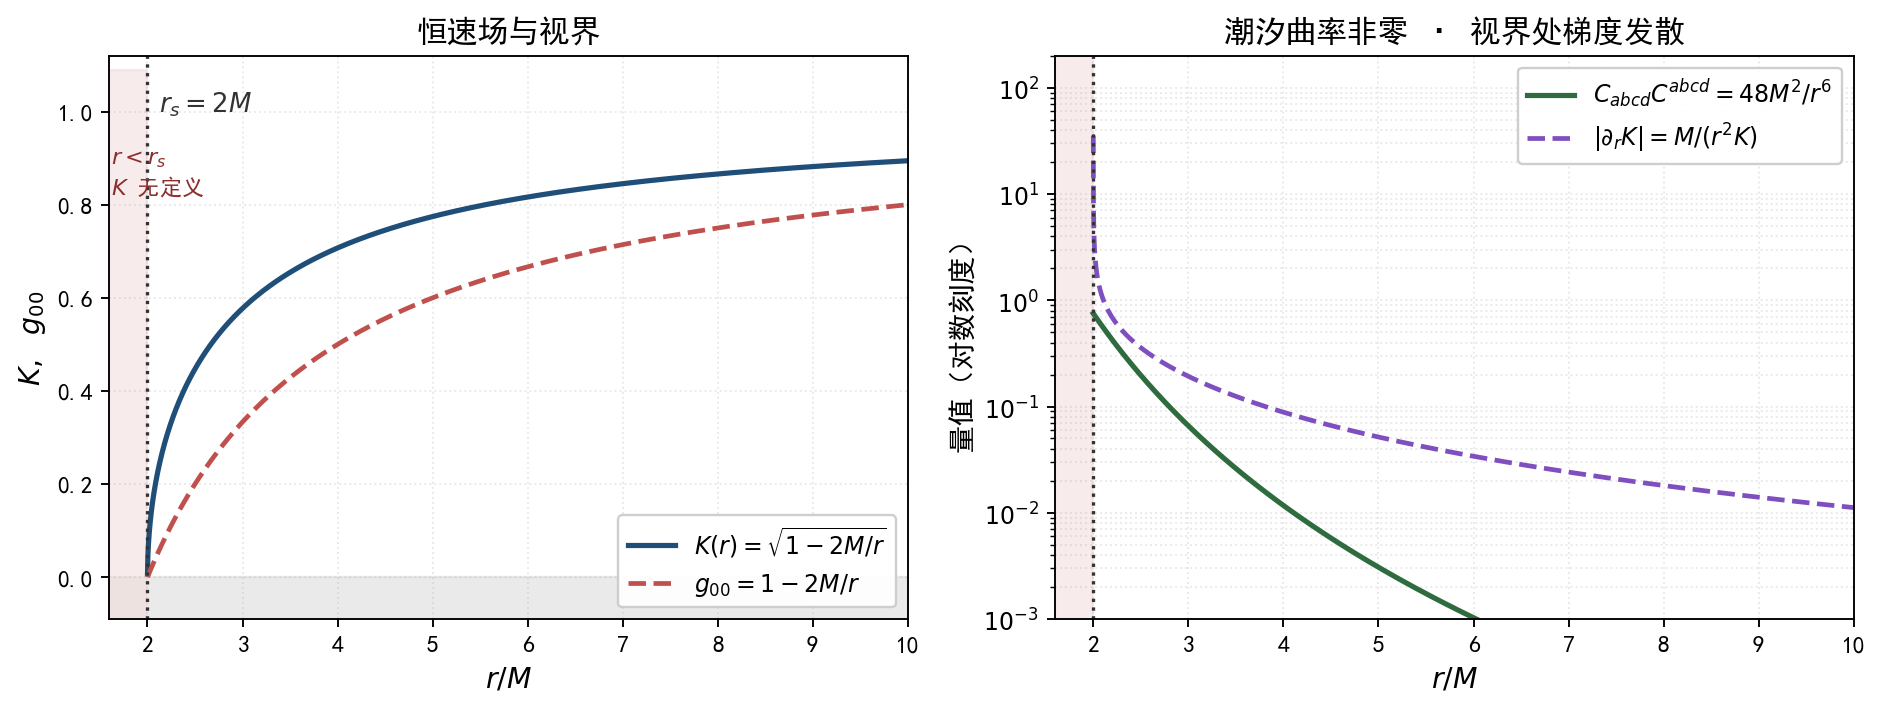
\includegraphics[width=0.86\linewidth,height=\textheight,keepaspectratio]{chapters/images/invariant-speed-horizon.png}

}

\caption{\label{fig-isg2-horizon}恒速场 \(K(r)\) 与 Schwarzschild 视界}

\end{figure}%

\section{黑洞视界的条件}\label{sec-isg2-horizon}

\subsection{两个不同的曲面}\label{ux4e24ux4e2aux4e0dux540cux7684ux66f2ux9762}

由 式~\ref{eq-isg2-adm}：

\[
g_{00}=K^{2}-h_{ij}\beta^{i}\beta^{j}
\]

在本章的族中
\(h_{ij}\beta^{i}\beta^{j}=r^{2}s^{2}\Omega^{2}=:\lvert\beta\rvert^{2}_{h}\)。

\textbf{(a) 静止限（无限红移面）}：

\begin{equation}\protect\phantomsection\label{eq-isg2-staticlimit}{
g_{00}=0\quad\Longleftrightarrow\quad K^{2}=\lvert\beta\rvert^{2}_{h}\quad\Longleftrightarrow\quad \boxed{\lvert\beta\rvert_{h}=K}
}\end{equation}

即：\textbf{拖曳速度在空间度规下的模长等于局部光速时，出现静止限。}
这是一条只用 \(K\) 与 \(\beta\) 表述的判据。

\textbf{(b) 事件视界（Killing 视界）}：对静态情形，事件视界位于
\(g^{rr}=0\)，由 式~\ref{eq-isg2-ginv} 即

\begin{equation}\protect\phantomsection\label{eq-isg2-eventhorizon}{
g^{rr}=-\frac{1}{A}=0\quad\Longleftrightarrow\quad \boxed{A^{-1}=0}
}\end{equation}

\subsection{Schwarzschild
情形：两者重合}\label{schwarzschild-ux60c5ux5f62ux4e24ux8005ux91cdux5408}

\(\Omega=0\) 时 \(\lvert\beta\rvert_{h}=0\)，由
式~\ref{eq-isg2-staticlimit} 得 \(K=0\)；而
式~\ref{eq-isg2-eventhorizon} 给出 \(A^{-1}=F=K^{2}=0\)，同样得

\[
K=0
\]

\textbf{两条判据在 \(\Omega=0\) 时给出同一个曲面。} 由
\(K^{2}=1-\dfrac{2M}{r}\)：

\[
K(r_s)=0\quad\Longrightarrow\quad 1-\frac{2M}{r_s}=0\quad\Longrightarrow\quad r_s=2M
\]

恢复量纲（\(M\to GM/c^{2}\)）：

\begin{equation}\protect\phantomsection\label{eq-isg2-rs}{
\boxed{r_s=\frac{2GM}{c^{2}},\qquad K(r)=\sqrt{1-\frac{2GM}{c^{2}r}}}
}\end{equation}

\textbf{这就是史瓦西半径，由恒速场 \(K\) 的零点给出。}

\subsection{\texorpdfstring{从 \(K\) 直接导出
Schwarzschild}{从 K 直接导出 Schwarzschild}}\label{ux4ece-k-ux76f4ux63a5ux5bfcux51fa-schwarzschild}

真空条件 + \(A=1/F\)（即 \(g^{rr}=-F\) 的静态球对称真空形式）⟹ 由
式~\ref{eq-isg2-R22}：

\[
R_{22}=-\frac{rF'}{2AF}+\frac{rA'}{2A^{2}}+1-\frac{1}{A}
\]

代入 \(A=1/F\)，\(A'=-F'/F^{2}\)：

\[
R_{22}=-\frac{rF'}{2}+\frac{r}{2}\cdot\frac{-F'/F^{2}}{1/F^{2}}+1-F
=-\frac{rF'}{2}-\frac{rF'}{2}+1-F=1-F-rF'
\]

真空要求 \(R_{22}=0\)：

\[
1-F-rF'=0\quad\Longleftrightarrow\quad rF'+F=1\quad\Longleftrightarrow\quad (rF)'=1
\]

积分：

\[
rF=r+C\quad\Longrightarrow\quad F=1+\frac{C}{r}
\]

取 \(C=-2M\)（使 \(r\to\infty\) 时 \(F\to1\)，即渐近处 \(K\to1\)）：

\begin{equation}\protect\phantomsection\label{eq-isg2-derive}{
\boxed{F=K^{2}=1-\frac{2M}{r}}
}\end{equation}

\textbf{链条闭合}：恒速场 \(K\) 的真空方程 \(\Longrightarrow\)
\(K^{2}=1-\frac{2M}{r}\) \(\Longrightarrow\) 视界 \(K=0\)
\(\Longrightarrow\) \(r_s=2M\)。

\subsection{视界处的梯度}\label{ux89c6ux754cux5904ux7684ux68afux5ea6}

\[
\frac{\mathrm{d}K}{\mathrm{d}r}=\frac{M}{r^{2}\sqrt{1-\dfrac{2M}{r}}}
\]

在 \(r\to r_s=2M\) 处 \(K\to0\) 而
\(\mathrm{d}K/\mathrm{d}r\to\infty\)：\textbf{视界处恒速场的梯度发散，\(\vec\nabla K\neq0\)
且无界。}

\section{量子力学在此背景下不适用}\label{sec-isg2-qm}

\textbf{声明}：本节是\textbf{否定性}的结论，不是兼容方案。在强引力背景下不求解薛定谔方程。

由上一节，黑洞解满足

\[
\vec\nabla K\neq0,\qquad \text{且在 } r\to r_s \text{ 处 } \lvert\vec\nabla K\rvert\to\infty
\]

而前一章已严格证明：当 \(\vec\nabla K\neq0\) 时，从变系数 Klein--Gordon
方程抽出快变相位 \(\theta=-mK^{2}t/\hbar\) 后，残留项

\[
\frac{4m^{2}t^{2}}{\hbar^{2}}\lvert\vec\nabla K\rvert^{2}\varphi
\]

在 \(K\to\infty\) 的极限下按 \(K_0^{2}\)
增长而\textbf{发散}，非相对论极限不存在。

\textbf{合起来}：

{\def\LTcaptype{none} % do not increment counter
\begin{longtable}[]{@{}
  >{\raggedright\arraybackslash}p{(\linewidth - 2\tabcolsep) * \real{0.5000}}
  >{\raggedright\arraybackslash}p{(\linewidth - 2\tabcolsep) * \real{0.5000}}@{}}
\toprule\noalign{}
\begin{minipage}[b]{\linewidth}\raggedright
条件
\end{minipage} & \begin{minipage}[b]{\linewidth}\raggedright
结论
\end{minipage} \\
\midrule\noalign{}
\endhead
\bottomrule\noalign{}
\endlastfoot
\(\vec\nabla K=0\) & 非相对论极限存在，薛定谔方程严格成立，Bargmann
中央扩张良定义 \\
\(\vec\nabla K\neq0\)（一切有引力的情形） &
非相对论极限\textbf{不存在}，薛定谔方程不适用 \\
\(r\to r_s\)（黑洞视界） &
\(\lvert\vec\nabla K\rvert\to\infty\)，上述发散最严重 \\
\end{longtable}
}

\textbf{因此}：在黑洞或任何 \(K\)
不均匀的引力背景下，量子力学（作为非相对论极限的产物）在数学上不能直接适用。\textbf{这不是需要修补的困难，而是两个相态的分界}：\(K\)
均匀且取 \(\infty\) 的一端是量子力学的相，\(K\)
不均匀的一端是引力的相，二者由不同的参数区域刻画，不在同一个非均匀背景上强行耦合。

\section{结论}\label{sec-isg2-conclusion}

\begin{longtable}[]{@{}
  >{\raggedright\arraybackslash}p{(\linewidth - 2\tabcolsep) * \real{0.5000}}
  >{\raggedright\arraybackslash}p{(\linewidth - 2\tabcolsep) * \real{0.5000}}@{}}
\caption{本章各命题及其依据}\label{tbl-isg2-conclusion}\tabularnewline
\toprule\noalign{}
\begin{minipage}[b]{\linewidth}\raggedright
命题
\end{minipage} & \begin{minipage}[b]{\linewidth}\raggedright
依据
\end{minipage} \\
\midrule\noalign{}
\endfirsthead
\toprule\noalign{}
\begin{minipage}[b]{\linewidth}\raggedright
命题
\end{minipage} & \begin{minipage}[b]{\linewidth}\raggedright
依据
\end{minipage} \\
\midrule\noalign{}
\endhead
\bottomrule\noalign{}
\endlastfoot
标架 \(=K\times\) 局部洛伦兹变换 ⟹ 共形平坦、Weyl\(\equiv0\) &
定理~\ref{thm-isg2-nogo} \\
完备分解 \(K+\beta^{i}+h_{ij}\) 有 \(1+3+6=10\) 个自由度 &
小节~\ref{sec-isg2-dof} \\
非对角项 \(g_{03}=-r^{2}s^{2}\Omega\) 来自拖曳 & 式~\ref{eq-isg2-g00} \\
\(K\) 常数、\(\beta=0\)、\(h\) 平坦 ⟹ Minkowski ⟹ 全局恒速群 &
小节~\ref{sec-isg2-degenerate} \\
旋转坐标自检（\(F=A=1\)、\(\Omega\) 常数）⟹ Weyl\(=0\) &
小节~\ref{sec-isg2-degenerate} \\
Christoffel \(15\) 个非零分量 & 式~\ref{eq-isg2-gamma} \\
Ricci \(5\) 个非零分量、Ricci 标量 &
式~\ref{eq-isg2-R00}---式~\ref{eq-isg2-Rscalar} \\
Einstein \(5\) 个非零分量，含完整的 \(G_{00}\) &
式~\ref{eq-isg2-G00}---式~\ref{eq-isg2-G33} \\
Weyl 一般非零 & 式~\ref{eq-isg2-C0101}---式~\ref{eq-isg2-C2323} \\
Schwarzschild：\(R_{\mu\nu}=0\)、\(G_{\mu\nu}=0\)、\(C_{abcd}C^{abcd}=48M^{2}/r^{6}\)
& 式~\ref{eq-isg2-I} \\
静止限 \(\lvert\beta\rvert_h=K\)；事件视界 \(A^{-1}=0\) &
式~\ref{eq-isg2-staticlimit}、式~\ref{eq-isg2-eventhorizon} \\
真空 ⟹ \(K^{2}=1-\frac{2M}{r}\)，视界 \(K=0\) ⟹ \(r_s=2M\) &
式~\ref{eq-isg2-derive}、式~\ref{eq-isg2-rs} \\
\(\vec\nabla K\neq0\) ⟹ 非相对论极限不存在 & 小节~\ref{sec-isg2-qm} \\
\end{longtable}

\textbf{一句话}：恒速场 \(K\) 本身只给出 \(1\) 个自由度，只能得到
Weyl\(\equiv0\) 的共形几何；把标架完备化（补上拖曳 \(\beta^{i}\) 与剪切
\(h_{ij}\)，\(1+3+6=10\)）后，Weyl 张量严格非零（Schwarzschild 处
\(C_{abcd}C^{abcd}=48M^{2}/r^{6}\)），并且真空方程直接给出
\(K^{2}=1-\frac{2M}{r}\)、视界由 \(K=0\) 定出为 \(r_s=2M\)；在同一背景下
\(\vec\nabla K\neq0\)，非相对论极限不存在，量子力学不适用。

\section{术语说明}\label{sec-isg2-terms}

{\def\LTcaptype{none} % do not increment counter
\begin{longtable}[]{@{}ll@{}}
\toprule\noalign{}
术语 & 本章中的含义 \\
\midrule\noalign{}
\endhead
\bottomrule\noalign{}
\endlastfoot
lapse \(K\) & ADM 分解中的时间尺度因子；本章即恒速场＝局部光速上限 \\
shift \(\beta^{i}\) & 空间坐标随时间的漂移（拖曳），产生
\(g_{0i}\neq0\) \\
剪切 & \(h_{ij}\) 中不可由共形因子吸收的各向异性部分 \\
静止限 & \(g_{00}=0\) 的曲面，等价于 \(\lvert\beta\rvert_h=K\) \\
事件视界 & 静态情形下的 Killing 视界，本章为 \(g^{rr}=0\) \\
Weyl 张量 & 度规中不因共形变换改变的部分，度量潮汐效应 \\
Weyl 不变量 & \(C_{abcd}C^{abcd}\)，Schwarzschild 处为
\(48M^{2}/r^{6}\) \\
\end{longtable}
}

\bookmarksetup{startatroot}

\chapter{量子相态的代数生成}\label{sec-quantum-phase}

\section{本章的范围}\label{sec-qp-scope}

\textbf{一句话}：取定相态参数（\(K\to\infty\) 且
\(\vec\nabla K=0\)），从恒速群 \(G_K\)
出发，经李代数收缩、射影表示与中央扩张，把量子力学的核心骨架（质量作为中央荷、\([q_i,p_j]=i\hbar\delta_{ij}\)、薛定谔方程）逐项推导出来；最后用反证法证明这个骨架在
\(\vec\nabla K\neq0\) 处不能存在。

\textbf{推导链条}：

\[
\begin{aligned}
\text{恒速群 } G_K\ \longrightarrow\ &\underbrace{K\to\infty,\ \vec\nabla K=0}_{\text{相态参数}}
\ \longrightarrow\ \text{伽利略群}\ \longrightarrow\ \text{射影表示 / 中央扩张}\\[4pt]
\longrightarrow\ &\text{Bargmann 代数}\ \longrightarrow\ \text{波动力学}\ \longrightarrow\ \text{量子力学骨架}
\end{aligned}
\]

\subsection{三条禁令（本章的自我约束）}\label{ux4e09ux6761ux7981ux4ee4ux672cux7ae0ux7684ux81eaux6211ux7ea6ux675f}

\begin{enumerate}
\def\labelenumi{\arabic{enumi}.}
\tightlist
\item
  \textbf{不出现弯曲度规}。本章全程 \(K\) 为常数，只用恒速群的不变二次型
  \(Q_K=K^{2}t^{2}-\lvert\mathbf{x}\rvert^{2}\) 及其对偶算符；不用任何
  \(g_{\mu\nu}(x)\)、不用 Christoffel 符号、不做度规量子化。
\item
  \textbf{不出现引力}。\(\vec\nabla K\neq0\)
  只在第四部分作为\textbf{反证法的假设}出现，且立即导致矛盾。
\item
  \textbf{不出现''量子引力''}。本章不构造任何''引力的量子理论''。第四部分的结论恰恰是：那样的对象在本框架内没有定义域。
\end{enumerate}

\subsection{禁止预设清单}\label{ux7981ux6b62ux9884ux8bbeux6e05ux5355}

以下内容在本章出现的\textbf{位置}被严格规定，此前不得使用：

{\def\LTcaptype{none} % do not increment counter
\begin{longtable}[]{@{}
  >{\raggedright\arraybackslash}p{(\linewidth - 2\tabcolsep) * \real{0.5000}}
  >{\raggedright\arraybackslash}p{(\linewidth - 2\tabcolsep) * \real{0.5000}}@{}}
\toprule\noalign{}
\begin{minipage}[b]{\linewidth}\raggedright
对象
\end{minipage} & \begin{minipage}[b]{\linewidth}\raggedright
首次出现
\end{minipage} \\
\midrule\noalign{}
\endhead
\bottomrule\noalign{}
\endlastfoot
薛定谔方程 & 式~\ref{eq-qp-schrodinger}（第三部分末尾） \\
对易关系 \([q_i,p_j]=i\hbar\delta_{ij}\) &
式~\ref{eq-qp-ccr}（第二部分末尾） \\
德布罗意关系 \(E=\hbar\omega\)、\(p=\hbar k\) &
式~\ref{eq-qp-debroglie}（第三部分） \\
质量 \(m\) & 式~\ref{eq-qp-m2}（作为质量壳参数引入，先于一切解释） \\
\end{longtable}
}

第一、二部分\textbf{不预设}薛定谔方程与对易关系；它们是被推出来的，不是被写下来的。

\subsection{记号与约定}\label{ux8bb0ux53f7ux4e0eux7ea6ux5b9a}

\begin{itemize}
\tightlist
\item
  \(K\)：恒速场（本章为常数）；\(K^{2}=F\)。
\item
  生成元：\textbf{Hermitian} 算符
  \(\hat H\)（时间平移）、\(\hat P_i\)（空间平移）、\(\hat B_i\)（boost）、\(\hat J_i\)（转动）、\(\hat M\)（中央荷）。位置算符记作
  \(\hat q_i\)，以免与 \(K\) 混淆。
\item
  向量场 \(X\) 与其 Hermitian
  算符的对应：\([\hat X,\hat Y]=i\hbar\,[X,Y]_{\text{vf}}\)。据此
  \(\hat P_i=-i\hbar\partial_i\)、\(\hat H=i\hbar\partial_t\)。
\item
  \(\hbar\) 的地位：量子化映射 \([\ ,\ ]=i\hbar\{\ ,\ \}\)
  的尺度，是经验常数；本章\textbf{不声称}推导它的数值。本章推导的是
  \(m\) 的地位。
\item
  符号核验脚本 \texttt{images/quantum-phase-algebra.py}，输出见
  \texttt{images/qp.out}；本章每个闭式后标注核验结果。
\end{itemize}

\section{\texorpdfstring{第一部分　相态参数：\(K\to\infty\) 与
\(\vec\nabla K=0\)}{第一部分　相态参数：K\textbackslash to\textbackslash infty 与 \textbackslash vec\textbackslash nabla K=0}}\label{sec-qp-part1}

\subsection{\texorpdfstring{恒速群的 \(K\to\infty\)
极限}{恒速群的 K\textbackslash to\textbackslash infty 极限}}\label{ux6052ux901fux7fa4ux7684-ktoinfty-ux6781ux9650}

第 章节~\ref{sec-invariant-speed-group} 章的恒速群 \(G_K\)（取 \(1+1\)
维，空间部分同理）：

\begin{equation}\protect\phantomsection\label{eq-qp-GK}{
t'=\frac{t-\dfrac{vx}{K^{2}}}{\sqrt{1-\dfrac{v^{2}}{K^{2}}}},\qquad
x'=\frac{x-vt}{\sqrt{1-\dfrac{v^{2}}{K^{2}}}}
}\end{equation}

\begin{proposition}[\(K\to\infty\)
逐项给出伽利略变换]\protect\hypertarget{prp-qp-galileo}{}\label{prp-qp-galileo}

在 式~\ref{eq-qp-GK} 中令 \(K\to\infty\)（\(v\) 固定），逐项取极限得

\[
t'=t,\qquad x'=x-vt
\]

即伽利略变换。

\end{proposition}

\textbf{证明}：\(\sqrt{1-v^{2}/K^{2}}\to1\)；\(\dfrac{vx}{K^{2}}\to0\)。故
\(t'\to t\)、\(x'\to x-vt\)。

符号核验（向量场层面）：boost 生成元
\(B=-\dfrac{x}{K^{2}}\partial_t-t\partial_x\) 在 \(K\to\infty\) 下给出
\((0,-t)\)，即 \(-t\partial_x\)；且 \([B,P]\) 的极限为 \((0,0)\)。输出：

\begin{verbatim}
K->oo 后 boost 生成元 B = (0, -t)
K->oo 后 [B,P] = (0, 0)
\end{verbatim}

\subsection{\texorpdfstring{不变量的退化：从 \(1\) 个到 \(2\)
个}{不变量的退化：从 1 个到 2 个}}\label{ux4e0dux53d8ux91cfux7684ux9000ux5316ux4ece-1-ux4e2aux5230-2-ux4e2a}

恒速群的不变量为

\[
Q_K=K^{2}(\Delta t)^{2}-\lvert\Delta\mathbf{x}\rvert^{2}
\]

两边除以 \(K^{2}\) 并取 \(K\to\infty\)：

\[
\frac{Q_K}{K^{2}}=(\Delta t)^{2}-\frac{\lvert\Delta\mathbf{x}\rvert^{2}}{K^{2}}\ \longrightarrow\ (\Delta t)^{2}
\]

所以极限结构不再由\textbf{一个}二次型给出，而由\textbf{两个}独立的不变量给出：

\begin{equation}\protect\phantomsection\label{eq-qp-two-invariants}{
\boxed{\Delta t\ \text{不变},\qquad \lvert\Delta\mathbf{x}\rvert\ \text{不变}}
}\end{equation}

\textbf{这就是''绝对时间 +
绝对空间''的严格含义}：时空不再是带单一度规的整体，而是
\(\mathbb{R}\times\mathbb{R}^{3}\)
上分别带时间尺度与欧氏尺度的一对结构。式~\ref{eq-qp-two-invariants}
是本章全部推导的几何输入。

\subsection{零锥的退化}\label{ux96f6ux9525ux7684ux9000ux5316}

零锥 \(\lvert\mathrm{d}\mathbf{x}/\mathrm{d}t\rvert=K\) 在
\(K\to\infty\) 时张开为

\[
\lvert\mathrm{d}\mathbf{x}/\mathrm{d}t\rvert=\infty\quad\Longleftrightarrow\quad t=\text{常数}
\]

即：\textbf{零曲面退化为同时超曲面}，信号速度无上界。这正是伽利略时空''瞬时传播''的严格表述，也是后面非相对论极限中''不存在不变波速''的几何根源。

\subsection{\texorpdfstring{\(\vec\nabla K=0\)
不是简化假设，而是前提}{\textbackslash vec\textbackslash nabla K=0 不是简化假设，而是前提}}\label{vecnabla-k0-ux4e0dux662fux7b80ux5316ux5047ux8bbeux800cux662fux524dux63d0}

第 章节~\ref{sec-invariant-speed-field-group} 章已证明：当 \(K\)
随点变化时，逐点的 \(G_{K(p)}\)
各自成群，但\textbf{跨点的复合不再是群运算}------复合多出
\(\propto\partial_\mu K/K\) 的项。

\textbf{本章第二部分要做的事是''表示论''}：表示论的对象是\textbf{一个群}。因此：

\[
\vec\nabla K\neq0\ \Longrightarrow\ \text{不存在可供表示的全局群}\ \Longrightarrow\ \text{第二部分全部失效}
\]

这不是''为了算得动而设的简化''，而是\textbf{定义域条件}：量子相态的定义本身就包含
\(\vec\nabla K=0\)。第四部分会把这一点写成反证法的第一层。

\subsection{不变算符与色散关系}\label{ux4e0dux53d8ux7b97ux7b26ux4e0eux8272ux6563ux5173ux7cfb}

由不变量 \(Q_K\) 的对偶（逆）二次型
\(\mathrm{diag}(K^{-2},-1,-1,-1)\)，恒速群的不变算符为

\begin{equation}\protect\phantomsection\label{eq-qp-box}{
\Box_K:=\frac{1}{K^{2}}\partial_t^{2}-\nabla^{2}
}\end{equation}

（\(K\)
为常数，故这是\textbf{平直}的常系数算符；本章不涉及任何变系数或弯曲版本。）

取 \(\psi\sim e^{i(\mathbf{k}\cdot\mathbf{x}-\omega t)}\)，代入
\((\Box_K+\text{质量项})\psi=0\)：

\[
-\frac{\omega^{2}}{K^{2}}+\lvert\mathbf{k}\rvert^{2}=-\frac{m^{2}K^{2}}{\hbar^{2}}
\]

以 \(E=\hbar\omega\)、\(p=\hbar\lvert\mathbf{k}\rvert\)
写出，得\textbf{恒速群的质量壳关系}：

\begin{equation}\protect\phantomsection\label{eq-qp-m2}{
\boxed{\frac{E^{2}}{K^{2}}-\lvert\mathbf{p}\rvert^{2}=m^{2}K^{2}}
\quad\Longleftrightarrow\quad
E^{2}=m^{2}K^{4}+\lvert\mathbf{p}\rvert^{2}K^{2}
}\end{equation}

式~\ref{eq-qp-m2} 中的 \(m\)
是质量壳参数；它的代数身份（本征值还是中央荷）由第二部分定出。

\section{第二部分　伽利略代数与中央扩张}\label{sec-qp-part2}

\subsection{恒速代数的收缩}\label{ux6052ux901fux4ee3ux6570ux7684ux6536ux7f29}

恒速群的生成元（向量场）：\(H=\partial_t\)、\(P_i=\partial_i\)、\(B_i=-\dfrac{x_i}{K^{2}}\partial_t-t\partial_i\)。符号核验给出

\[
[B_i,P_j]=\frac{\delta_{ij}}{K^{2}}H,\qquad [B_i,H]=P_i,\qquad [H,P_i]=0
\]

换成 Hermitian 算符（\([\hat X,\hat Y]=i\hbar[X,Y]_{\text{vf}}\)）：

\begin{equation}\protect\phantomsection\label{eq-qp-algK}{
[\hat B_i,\hat P_j]=\frac{i\hbar}{K^{2}}\delta_{ij}\hat H,\qquad
[\hat B_i,\hat H]=i\hbar\hat P_i,\qquad
[\hat H,\hat P_i]=[\hat P_i,\hat P_j]=[\hat B_i,\hat B_j]=0
}\end{equation}

全部结构常数中 \(K\) 只以 \(1/K^{2}\) 出现（第
章节~\ref{sec-invariant-speed-group} 章的结论）。

\begin{theorem}[朴素收缩]\protect\hypertarget{thm-qp-contraction}{}\label{thm-qp-contraction}

若在 式~\ref{eq-qp-algK} 中令 \(K\to\infty\) 而保持 \(\hat H\) 有限，则

\[
[\hat B_i,\hat P_j]\to0
\]

所得的正是\textbf{无中央扩张的伽利略代数}（\(10\) 个生成元
\(\hat H,\hat P_i,\hat B_i,\hat J_i\)）：

\begin{equation}\protect\phantomsection\label{eq-qp-gal}{
[\hat B_i,\hat H]=i\hbar\hat P_i,\quad [\hat B_i,\hat P_j]=0,\quad
[\hat H,\hat P_i]=0,\quad [\hat P_i,\hat P_j]=0,\quad [\hat B_i,\hat B_j]=0
}\end{equation}

\end{theorem}

\textbf{但这是一个陷阱。} 在质量壳 式~\ref{eq-qp-m2} 上，\(\hat H\)
的谱为

\begin{equation}\protect\phantomsection\label{eq-qp-expE}{
E=\sqrt{m^{2}K^{4}+\lvert\mathbf{p}\rvert^{2}K^{2}}
=mK^{2}\sqrt{1+\frac{\lvert\mathbf{p}\rvert^{2}}{m^{2}K^{2}}}
=mK^{2}+\frac{\lvert\mathbf{p}\rvert^{2}}{2m}+O\!\left(\frac{1}{K^{2}}\right)
}\end{equation}

即 \(\hat H\)
\textbf{不保持有限}：\(\hat H/K^{2}\to m\cdot\mathbf 1\)。\(\hat H\)
发散而结构常数 \(1/K^{2}\) 消失，两者相乘留下有限的非零极限。这就是
Inönü--Wigner 收缩中的\textbf{重整化收缩}。

\begin{theorem}[中央荷的诞生]\protect\hypertarget{thm-qp-central}{}\label{thm-qp-central}

在质量壳 式~\ref{eq-qp-m2} 的表示上作重整化收缩

\[
\hat B_i\ \text{不变},\qquad \hat P_i\ \text{不变},\qquad
\hat H_{\text{nr}}:=\hat H-mK^{2}\mathbf 1
\]

则 \(K\to\infty\) 时

\[
[\hat B_i,\hat P_j]=\frac{i\hbar}{K^{2}}\delta_{ij}\bigl(mK^{2}\mathbf 1+\hat H_{\text{nr}}\bigr)
=i\hbar\delta_{ij}m\,\mathbf 1+\frac{i\hbar}{K^{2}}\delta_{ij}\hat H_{\text{nr}}
\ \longrightarrow\ \boxed{i\hbar\delta_{ij}\hat M},\qquad \hat M:=m\,\mathbf 1
\]

同时

\[
[\hat B_i,\hat H_{\text{nr}}]=[\hat B_i,\hat H]=i\hbar\hat P_i,\qquad
[\hat P_i,\hat H_{\text{nr}}]=0
\]

所得的代数\textbf{不是} 式~\ref{eq-qp-gal}，而是带中央扩张的
\textbf{Bargmann 代数}。

\end{theorem}

\textbf{证明}：第一式用 \(\hat H=mK^{2}\mathbf 1+\hat H_{\text{nr}}\)
代入 式~\ref{eq-qp-algK}；第二式用 \([mK^{2}\mathbf 1,\cdot]=0\)。极限中
\(\hat H_{\text{nr}}/K^{2}\to0\)。

\textbf{收敛核验}：由 式~\ref{eq-qp-m2} 与
\(\hat H=mK^{2}+\hat H_{\text{nr}}\)，

\begin{equation}\protect\phantomsection\label{eq-qp-casimir-contract}{
\frac{\hat H^{2}}{K^{2}}-\lvert\hat{\mathbf P}\rvert^{2}=m^{2}K^{2}
\ \Longrightarrow\ 2m\hat H_{\text{nr}}-\lvert\hat{\mathbf P}\rvert^{2}+\frac{\hat H_{\text{nr}}^{2}}{K^{2}}=0
\ \xrightarrow{K\to\infty}\ \boxed{\hat H_{\text{nr}}=\frac{\lvert\hat{\mathbf P}\rvert^{2}}{2m}}
}\end{equation}

符号核验输出：\texttt{展开\ E\^{}2/K\^{}2\ -\ p\^{}2\ -\ m\^{}2K\^{}2\ =\ E\_nr**2/K**2\ +\ 2*E\_nr*m\ -\ p**2}，极限为
\texttt{2*E\_nr*m\ -\ p**2}。

\subsection{经典实现已经带着中央荷}\label{ux7ecfux5178ux5b9eux73b0ux5df2ux7ecfux5e26ux7740ux4e2dux592eux8377}

在相空间 \((\mathbf q,\mathbf p)\) 上，伽利略 boost 要求

\[
\delta q_i=v_i t,\qquad \delta p_i=m v_i
\]

由泊松括号生成：\(\delta f=\{\mathbf v\cdot\mathbf K,f\}\)，解出

\begin{equation}\protect\phantomsection\label{eq-qp-Kclass}{
\mathbf K=m\mathbf q-t\mathbf p
}\end{equation}

（校核：\(\{v_jK_j,q_i\}=v_j\{mq_j-tp_j,q_i\}=tv_i\)；\(\{v_jK_j,p_i\}=v_j m\delta_{ji}=mv_i\)。）

于是

\begin{equation}\protect\phantomsection\label{eq-qp-poisson}{
\boxed{\{K_i,p_j\}=m\,\delta_{ij}\neq0}
}\end{equation}

\textbf{这是关键的一步}：伽利略群在\textbf{经典}相空间上的实现，其 boost
生成元与动量的括号\textbf{已经非零}，数值就是
\(m\)。换言之，\textbf{经典理论早就活在中央扩张里}，只是没有人这样叫它。量子化映射
\([\ ,\ ]=i\hbar\{\ ,\ \}\) 于是直接给出

\[
[\hat B_i,\hat P_j]=i\hbar\delta_{ij}m\,\mathbf 1
\]

与 定理~\ref{thm-qp-central} 完全一致。两条独立的路（代数收缩 /
经典实现）给出同一个中央荷。

\subsection{中央扩张的分类：唯一性}\label{ux4e2dux592eux6269ux5f20ux7684ux5206ux7c7bux552fux4e00ux6027}

\begin{theorem}[伽利略代数的中央扩张唯一]\protect\hypertarget{thm-qp-extension}{}\label{thm-qp-extension}

设 \(\mathfrak g\) 为 式~\ref{eq-qp-gal} 的伽利略代数（生成元
\(\hat H,\hat P_i,\hat B_i,\hat J_i\)，共 \(10\)
个），其最一般的（一维）中央扩张为

\[
[X,Y]_{\text{ext}}=[X,Y]+c(X,Y)\,\hat M,\qquad [\hat M,\cdot]=0
\]

其中 \(c\) 为反对称双线性形。则 Jacobi
恒等式与''模去上边界''之后，解空间为

\[
\boxed{H^{2}(\mathfrak g,\mathbb R)=\mathbb R\ (\text{一维})}
\]

其非平凡代表元唯一（差一个常数倍）：

\begin{equation}\protect\phantomsection\label{eq-qp-cocycle}{
c(\hat B_i,\hat P_j)=\delta_{ij},\qquad \text{其余分量}=0
}\end{equation}

\end{theorem}

\textbf{证明（分四步）}：

\textbf{第一步（转动部分可清空）}。转动子代数 \(\mathfrak{so}(3)\)
半单，由 Whitehead 引理 \(H^{2}(\mathfrak{so}(3),\mathbb R)=0\)；又
\(\mathfrak{so}(3)\) 紧致，可对上闭链作平均而不改变其上同调类。故可取
\(c\) 为 \(\mathfrak{so}(3)\) 不变的，于是 \(c\) 的分量只能由不变张量
\(\delta_{ij}\)、\(\varepsilon_{ijk}\) 构造。

\textbf{第二步（逐分量消去）}。\(c\)
反对称，且取值是一维中心（无指标），故：

{\def\LTcaptype{none} % do not increment counter
\begin{longtable}[]{@{}
  >{\raggedright\arraybackslash}p{(\linewidth - 4\tabcolsep) * \real{0.3333}}
  >{\raggedright\arraybackslash}p{(\linewidth - 4\tabcolsep) * \real{0.3333}}
  >{\raggedright\arraybackslash}p{(\linewidth - 4\tabcolsep) * \real{0.3333}}@{}}
\toprule\noalign{}
\begin{minipage}[b]{\linewidth}\raggedright
分量
\end{minipage} & \begin{minipage}[b]{\linewidth}\raggedright
可用的不变张量
\end{minipage} & \begin{minipage}[b]{\linewidth}\raggedright
结论
\end{minipage} \\
\midrule\noalign{}
\endhead
\bottomrule\noalign{}
\endlastfoot
\(c(\hat P_i,\hat P_j)\)、\(c(\hat B_i,\hat B_j)\) & 反对称 \(2\)
阶不变张量不存在（\(\delta\) 对称、\(\varepsilon\) 需 \(3\) 个指标） &
\(=0\) \\
\(c(\hat H,\hat P_i)\)、\(c(\hat H,\hat B_i)\) & 不变矢量不存在 &
\(=0\) \\
\(c(\hat H,\hat J_i)=\eta\) & 标量，暂留 & 待定 \\
\(c(\hat J_i,\hat P_j)=\alpha\delta_{ij}\) & \(\delta\) 不变，暂留 &
待定 \\
\(c(\hat J_i,\hat B_j)=\gamma\delta_{ij}\) & 同上 & 待定 \\
\(c(\hat B_i,\hat P_j)=\beta\delta_{ij}\) & 同上，暂留 & 待定 \\
\end{longtable}
}

\textbf{第三步（Jacobi 杀死 \(\eta,\alpha,\gamma\)）}。

\begin{itemize}
\tightlist
\item
  对三元组 \((\hat H,\hat J_i,\hat J_j)\)： \[
  [\hat H,[\hat J_i,\hat J_j]]+[\hat J_i,[\hat J_j,\hat H]]+[\hat J_j,[\hat H,\hat J_i]]
  =\varepsilon_{ijk}[\hat H,\hat J_k]=\varepsilon_{ijk}\eta\,\hat M=0\ \Longrightarrow\ \eta=0
  \]
\item
  对 \((\hat J_i,\hat J_j,\hat P_k)\)：逐项展开（\(\varepsilon\)
  收缩恒等式
  \(\varepsilon_{jkl}\varepsilon_{ilm}-\varepsilon_{ikl}\varepsilon_{jlm}+\varepsilon_{ijl}\varepsilon_{klm}=0\)）后
  \(\hat P\) 项自动抵消，\(\hat M\) 项给出 \[
  \alpha\bigl(\varepsilon_{jki}-\varepsilon_{ikj}-\varepsilon_{ijk}\bigr)\hat M=\alpha\,\varepsilon_{ijk}\hat M=0\ \Longrightarrow\ \alpha=0
  \]
\item
  同理对 \((\hat J_i,\hat J_j,\hat B_k)\) 得
  \(\gamma\,\varepsilon_{ijk}=0\Longrightarrow\gamma=0\)。
\end{itemize}

\textbf{第四步（\(\beta\) 自由且非上边界）}。其余 Jacobi 恒等式对
\(\beta\) 无约束：

\begin{itemize}
\tightlist
\item
  \((\hat H,\hat B_i,\hat P_j)\)：\([\hat H,\beta\delta_{ij}\hat M]+[\hat B_i,0]+[\hat P_j,-i\hbar\hat P_i]=0\)；
\item
  \((\hat B_i,\hat B_j,\hat P_l)\)、\((\hat B_i,\hat P_j,\hat P_l)\)：\(\hat M\)
  为中心，全为零。
\end{itemize}

上边界形如 \(c_f(X,Y)=f([X,Y])\)（\(f\) 为线性泛函）。但
\([\hat B_i,\hat P_j]=0\)，故对任何 \(f\) 都有
\(c_f(\hat B_i,\hat P_j)=f(0)=0\neq\beta\delta_{ij}\)。故 \(\beta\neq0\)
时该上闭链\textbf{不是上边界}，上同调类非平凡。

\textbf{符号核验}（\(10\) 生成元、\(45\) 个待定分量、\(120\) 个 Jacobi
方程，逐一解出）：

\begin{verbatim}
未扩张伽利略代数 Jacobi 自检: True
2-闭上链空间维数: 10
2-上边界空间维数: 9
H^2(galilei, R) 的维数 = 1
代表元 c(P_i,K_j)=delta_ij 满足全部 Jacobi: True
上边界在 (K_i,P_j) 分量上的值 [K_i,P_j] = {} -> 恒为 0，故代表元非上边界
\end{verbatim}

\textbf{结论}：伽利略代数的中央扩张不是可以随意添加的附加结构，而是\textbf{唯一的、且非加不可的}（前提是质量非零）。

\subsection{射影表示与 Bargmann
群}\label{ux5c04ux5f71ux8868ux793aux4e0e-bargmann-ux7fa4}

\subsubsection{为什么必须射影}\label{ux4e3aux4ec0ux4e48ux5fc5ux987bux5c04ux5f71}

\textbf{理由一（量子力学的基本结构）}。物理态是 Hilbert
空间中的\textbf{射线}（Born 规则只依赖
\(\lvert\psi\rvert^{2}\)，全局相位不可观测）。由 Wigner
定理，对称群在射线上实现为酉（或反酉）变换，故只要求

\begin{equation}\protect\phantomsection\label{eq-qp-projective}{
U(g_2)U(g_1)=\omega(g_2,g_1)\,U(g_2g_1),\qquad \lvert\omega\rvert=1
}\end{equation}

即\textbf{射影表示}。上同调分类（定理~\ref{thm-qp-extension}）告诉我们：\(\omega\)
的非平凡部分只有一个参数。

\textbf{理由二（真表示不够用）}。若坚持
\(\omega\equiv1\)（真表示），则中央荷 \(\hat M=0\)，后果有三（见
小节~\ref{sec-qp-ccr}）：位置算符无从定义；\(\hat H_{\text{nr}}=\lvert\hat{\mathbf P}\rvert^{2}/2\hat M\)
无意义；且波方程在 boost 下不协变------符号核验给出：去掉相位后

\[
i\hbar\partial_t\Phi+\frac{\hbar^{2}}{2m}\partial_x^{2}\Phi
=i\hbar\partial_t\psi+\frac{\hbar^{2}}{2m}\partial_x^{2}\psi-i\hbar v\,\partial_x\psi
\]

残留项
\(-i\hbar v\,\partial_x\psi\neq0\)（\texttt{残留\ =\ -I*V*hbar*psi\_X}）。\textbf{故相位不是装饰，而是协变性的必要条件。}

\textbf{理由三（经典理论已经如此）}。式~\ref{eq-qp-poisson}
表明经典实现本身就带 \(m\)；量子化不能把一个非零的括号变成零。

\subsubsection{显式的上闭链}\label{ux663eux5f0fux7684ux4e0aux95edux94fe}

伽利略群元素 \(g=(b,\mathbf a,\mathbf v,R)\)，作用为

\[
\mathbf x'=R\mathbf x+\mathbf v t+\mathbf a,\qquad t'=t+b
\]

设波函数按

\begin{equation}\protect\phantomsection\label{eq-qp-Ug}{
(U(g)\psi)(\mathbf x',t')=\exp\!\left[\frac{i}{\hbar}m\Bigl(\mathbf v\cdot R\mathbf x+\frac{1}{2}\lvert\mathbf v\rvert^{2}t\Bigr)\right]\psi(\mathbf x,t)
}\end{equation}

（\(R=1\)、\(\mathbf a=0\)、\(b=0\) 时即
\(\psi'(\mathbf x,t)=e^{\frac{i}{\hbar}m(\mathbf v\cdot\mathbf x-\frac12 v^{2}t)}\psi(\mathbf x-\mathbf v t,t)\)，见
式~\ref{eq-qp-boost}。）

\textbf{复合计算}。连续作用 \(g_1\)、\(g_2\) 后总相位为

\[
\frac{m}{\hbar}\Bigl[\mathbf v_2\cdot R_2\mathbf x_1+\tfrac12\lvert\mathbf v_2\rvert^{2}t_1
+\mathbf v_1\cdot R_1\mathbf x+\tfrac12\lvert\mathbf v_1\rvert^{2}t\Bigr]
\]

代入
\(\mathbf x_1=R_1\mathbf x+\mathbf v_1t+\mathbf a_1\)、\(t_1=t+b_1\)，整理出
\(\mathbf x\) 与 \(t\) 的系数，与直接作用 \(U(g_2g_1)\)（其
\(\mathbf v=\mathbf v_2+R_2\mathbf v_1\)、\(R=R_2R_1\)）的相位逐项比较，二者\textbf{完全一致}，只差一个常数：

\begin{equation}\protect\phantomsection\label{eq-qp-cocycle-explicit}{
\boxed{U(g_2)U(g_1)=e^{\frac{i}{\hbar}m\,\xi(g_2,g_1)}U(g_2g_1)},\qquad
\xi(g_2,g_1)=\mathbf v_2\cdot R_2\mathbf a_1+\frac{1}{2}\lvert\mathbf v_2\rvert^{2}b_1
}\end{equation}

取
\(\mathbf v_2=\varepsilon\mathbf e_i\)、\(\mathbf a_1=\eta\mathbf e_j\)（\(b_1=0\)、\(R=I\)），得
\(\xi=\varepsilon\eta\delta_{ij}\)，其无穷小形式正是
\([\hat B_i,\hat P_j]=i\hbar\delta_{ij}\hat M\)。

\subsubsection{Bargmann 群}\label{bargmann-ux7fa4}

把相位升格为一个新的坐标 \(\zeta\)，定义
\(\mathbb R^{4}\times\mathbb R\) 上的作用

\[
\mathbf x'=R\mathbf x+\mathbf v t+\mathbf a,\qquad t'=t+b,\qquad
\zeta'=\zeta-\Bigl(\mathbf v\cdot R\mathbf x+\tfrac12\lvert\mathbf v\rvert^{2}t\Bigr)+c
\]

复合给出
\(c=c_1+c_2-\bigl(\tfrac12\lvert\mathbf v_2\rvert^{2}b_1+\mathbf v_2\cdot R_2\mathbf a_1\bigr)\)：这是\textbf{真正的群律}（结合律由构造保证），称为
\textbf{Bargmann 群} \(\widetilde G\)。它比伽利略群多一个中心方向
\(\zeta\)，其李代数正是 定理~\ref{thm-qp-central} 的扩张代数。

波函数取等变函数

\[
\widetilde\psi(\mathbf x,t,\zeta)=e^{\frac{i}{\hbar}m\zeta}\,\psi(\mathbf x,t)
\]

由 \(\widetilde\psi(gP)=\widetilde\psi(P)\) 反解，恰好回到
式~\ref{eq-qp-Ug}。\textbf{故''带相位的量子波函数''=``Bargmann
群中心方向上的等变函数''}，中央荷 \(m\) 就是该中心方向的本征值。

\subsection{质量的身份：中心元，而非本征值}\label{sec-qp-mass}

\begin{theorem}[质量的代数身份]\protect\hypertarget{thm-qp-mass}{}\label{thm-qp-mass}

在 \(K\to\infty\) 的相态中，质量 \(m\) 是李代数的\textbf{中心元素}
\(\hat M=m\mathbf 1\) 的本征值；而在 \(K\) 有限时，质量是
\textbf{Casimir 算符的本征值}。二者身份不同。

\end{theorem}

\textbf{证明（对照两条路）}：

\textbf{(a) \(K\) 有限（恒速群，含 \(K=c\) 的洛伦兹情形）}。由
式~\ref{eq-qp-m2}，

\[
\hat C:=\frac{\hat H^{2}}{K^{2}}-\lvert\hat{\mathbf P}\rvert^{2}=m^{2}K^{2}\mathbf 1
\]

\(\hat C\) 与所有生成元对易，是 Casimir 算符；\(m^{2}\)
是它的\textbf{本征值}。质量在这里是''由生成元算出来的一个数''：\(\hat C\)
由 \(\hat H,\hat{\mathbf P}\) 构造，\(m\) 由 \(\hat C\)
决定。\textbf{没有任何中心扩张}（\(H^{2}(\mathfrak{iso}(1,3),\mathbb R)=0\)，庞加莱群的射影表示等价于其万有覆盖的真表示）。

\textbf{(b) \(K\to\infty\)}。取极限后 \(\hat C=m^{2}K^{2}\to\infty\)
退化，式~\ref{eq-qp-casimir-contract} 给出存活的 Casimir

\begin{equation}\protect\phantomsection\label{eq-qp-casimirG}{
\hat C_{\text{G}}:=2\hat M\hat H_{\text{nr}}-\lvert\hat{\mathbf P}\rvert^{2}=2m\,\hat E_{\text{int}}
}\end{equation}

（校核：\([\hat B_l,\hat C_{\text{G}}]=2\hat M[\hat B_l,\hat H_{\text{nr}}]-[\hat B_l,\lvert\hat{\mathbf P}\rvert^{2}]=2\hat M(i\hbar\hat P_l)-2i\hbar\hat M\hat P_l=0\)。）

此时 \textbf{\(\hat M\) 本身是中心元素，不是任何算符的函数}：它不能由
\(\hat H,\hat P_i,\hat B_i,\hat J_i\) 表出（定理~\ref{thm-qp-extension}
的第四步），而是代数的一个独立方向。真正作为''本征值''出现的量换成了\textbf{内能}
\(\hat E_{\text{int}}\)。

\textbf{推论（Bargmann 超选择规则）}。\(\hat M\) 中心 \(\Rightarrow\) 由
Schur 引理，在不可约表示上 \(\hat M=m\mathbf 1\)；不同 \(m\)
的表示之间不存在把它们耦合起来的代数元素，故\textbf{不同质量的态不能相干叠加}------这是质量作为中央荷的可检验后果。相反，在
(a) 中 \(m\) 只是 Casimir
本征值，不同质量的态可以叠加。\textbf{``质量是中央荷''不是措辞，是有判别力的命题。}

{\def\LTcaptype{none} % do not increment counter
\begin{longtable}[]{@{}
  >{\raggedright\arraybackslash}p{(\linewidth - 4\tabcolsep) * \real{0.3333}}
  >{\raggedright\arraybackslash}p{(\linewidth - 4\tabcolsep) * \real{0.3333}}
  >{\raggedright\arraybackslash}p{(\linewidth - 4\tabcolsep) * \real{0.3333}}@{}}
\toprule\noalign{}
\begin{minipage}[b]{\linewidth}\raggedright
相态
\end{minipage} & \begin{minipage}[b]{\linewidth}\raggedright
\(m\) 的代数身份
\end{minipage} & \begin{minipage}[b]{\linewidth}\raggedright
可否叠加不同 \(m\)
\end{minipage} \\
\midrule\noalign{}
\endhead
\bottomrule\noalign{}
\endlastfoot
\(K\) 有限 & Casimir
\(\hat H^{2}/K^{2}-\lvert\hat{\mathbf P}\rvert^{2}\) 的本征值
\(m^{2}K^{2}\) & 可以 \\
\(K\to\infty\)、\(\vec\nabla K=0\) & \textbf{中心元素} \(\hat M\)
的本征值 \(m\) & \textbf{不可以}（超选择） \\
\end{longtable}
}

\subsection{位置--动量对易关系的导出}\label{sec-qp-ccr}

由 式~\ref{eq-qp-Kclass}，boost 生成元在 \(t=0\)
时等于''\(m\times\)位置''。据此\textbf{定义}位置算符：

\begin{equation}\protect\phantomsection\label{eq-qp-defq}{
\hat q_i:=\frac{1}{m}\bigl(\hat B_i+t\,\hat P_i\bigr)\qquad\Bigl(\text{即 } \hat B_i=m\hat q_i-t\hat P_i\Bigr)
}\end{equation}

\begin{theorem}[对易关系]\protect\hypertarget{thm-qp-ccr}{}\label{thm-qp-ccr}

在中央荷 \(\hat M=m\mathbf 1\) 的不可约扇区上，

\begin{equation}\protect\phantomsection\label{eq-qp-ccr}{
\boxed{[\hat q_i,\hat P_j]=i\hbar\delta_{ij}\mathbf 1}
}\end{equation}

\end{theorem}

\textbf{证明}：由 式~\ref{eq-qp-defq} 与 定理~\ref{thm-qp-central}，

\[
[\hat q_i,\hat P_j]=\frac{1}{m}\bigl[\hat B_i+t\hat P_i,\hat P_j\bigr]
=\frac{1}{m}\bigl[\hat B_i,\hat P_j\bigr]
=\frac{1}{m}\,i\hbar\delta_{ij}\hat M
=\frac{1}{m}\,i\hbar\delta_{ij}\,m\mathbf 1=i\hbar\delta_{ij}\mathbf 1
\]

（用到 \([\hat P_i,\hat P_j]=0\)。）

\textbf{显式算子核验}（\(\hat B=mx+i\hbar t\partial_x\)、\(\hat P=-i\hbar\partial_x\)、\(\hat q=x\)）：

\begin{verbatim}
[K,P] f = I*hbar*m*f(X, T) 期望 i hbar m f
[q,P] f = I*hbar*f(X, T) 期望 i hbar f
\end{verbatim}

\textbf{反之，若中央荷为零}（定理~\ref{thm-qp-contraction}
的朴素收缩）：\([\hat B_i,\hat P_j]=0\)，于是
\([\hat q_i,\hat P_j]=0\)。此时 \(\hat q\) 与 \(\hat P\)
可同时对角化：\textbf{没有不确定性原理，没有不可对易的观测量，量子化无从谈起}。这正是''伽利略代数本身
\([x,p]=0\)、无法支撑量子化''的严格形式------缺的不是某个技巧，缺的是中央扩张。

\textbf{推论（不确定性）}：由 式~\ref{eq-qp-ccr} 与
Cauchy--Schwarz，\(\Delta q_i\,\Delta P_i\geq\dfrac{\hbar}{2}\)。\(\hbar\)
在此第一次以''不可对易性的尺度''出现。

\section{第三部分　波动力学方程的生成}\label{sec-qp-part3}

\subsection{路线一：从 Casimir
直接生成}\label{ux8defux7ebfux4e00ux4ece-casimir-ux76f4ux63a5ux751fux6210}

在不可约表示上代入 式~\ref{eq-qp-casimirG}，并用
\(\hat H_{\text{nr}}=i\hbar\partial_t\)、\(\hat P_i=-i\hbar\partial_i\)、\(\hat M=m\mathbf 1\)：

\[
\Bigl(2m\,i\hbar\partial_t+\hbar^{2}\nabla^{2}\Bigr)\psi=2mE_{\text{int}}\psi
\]

无内部结构（\(E_{\text{int}}=0\)，即能量零点取在静能之上）时：

\begin{equation}\protect\phantomsection\label{eq-qp-schrodinger}{
i\hbar\partial_t\psi=-\frac{\hbar^{2}}{2m}\nabla^{2}\psi
}\end{equation}

\textbf{这就是薛定谔方程}------它是''\(\hat H_{\text{nr}}\) 由
\(\hat{\mathbf P}\) 与 \(\hat M\) 经 Casimir
决定''这一表示论事实的解析表达。

\subsection{路线二：从不变波动方程取极限（相位抽取，完整计算）}\label{ux8defux7ebfux4e8cux4eceux4e0dux53d8ux6ce2ux52a8ux65b9ux7a0bux53d6ux6781ux9650ux76f8ux4f4dux62bdux53d6ux5b8cux6574ux8ba1ux7b97}

由 式~\ref{eq-qp-box} 与质量壳 式~\ref{eq-qp-m2}，恒速群的不变波动方程为

\begin{equation}\protect\phantomsection\label{eq-qp-KG}{
\left(\frac{1}{K^{2}}\partial_t^{2}-\nabla^{2}+\frac{m^{2}K^{2}}{\hbar^{2}}\right)\psi=0
}\end{equation}

（\(K\) 为常数，平直，常系数。）注意 式~\ref{eq-qp-expE}：静能
\(mK^{2}\to\infty\)，故 \(\psi\) 含快变相位。抽取正能支：

\[
\psi=e^{-\frac{i}{\hbar}mK^{2}t}\,\varphi,\qquad
\theta:=\frac{mK^{2}t}{\hbar}
\]

逐项：

\[
\partial_t^{2}\psi=e^{-i\theta}\Bigl(\partial_t^{2}\varphi-\frac{2imK^{2}}{\hbar}\partial_t\varphi-\frac{m^{2}K^{4}}{\hbar^{2}}\varphi\Bigr)
\]

代入 式~\ref{eq-qp-KG}，\textbf{静能项严格相消}：

\[
\frac{1}{K^{2}}\Bigl(-\frac{m^{2}K^{4}}{\hbar^{2}}\varphi\Bigr)+\frac{m^{2}K^{2}}{\hbar^{2}}\varphi
=-\frac{m^{2}K^{2}}{\hbar^{2}}\varphi+\frac{m^{2}K^{2}}{\hbar^{2}}\varphi=0
\]

符号核验：\texttt{静能项\ m\^{}2K\^{}2/hbar\^{}2\ 是否相消（core\ -\ claim）:\ 0}。余下

\[
\frac{1}{K^{2}}\partial_t^{2}\varphi-\frac{2im}{\hbar}\partial_t\varphi-\nabla^{2}\varphi=0
\]

乘以 \(\dfrac{i\hbar}{2m}\) 并整理：

\begin{equation}\protect\phantomsection\label{eq-qp-preSch}{
i\hbar\partial_t\varphi=-\frac{\hbar^{2}}{2m}\nabla^{2}\varphi
+\frac{\hbar^{2}}{2mK^{2}}\partial_t^{2}\varphi
}\end{equation}

\textbf{取 \(K\to\infty\)，末项 \(\to0\)，得
式~\ref{eq-qp-schrodinger}。} 误差项是
\(\dfrac{\hbar^{2}}{2mK^{2}}\partial_t^{2}\varphi=O(K^{-2})\)，显式可控。

\textbf{两点说明}：

\begin{enumerate}
\def\labelenumi{\arabic{enumi}.}
\tightlist
\item
  相位 \(e^{-imK^{2}t/\hbar}\) 的选择 =
  正能支的选择；反号则取负能支。\(K\to\infty\)
  时两支被无穷大的静能间隙隔开，\textbf{反粒子在极限中消失}------这是相态边界的另一条痕迹。
\item
  静能 \(mK^{2}\)
  本身在极限中不收敛，它没有可观测量对应；它的''残余''正是中央荷
  \(\hat M=m\mathbf 1\)。定理~\ref{thm-qp-central}
  与这里的相消是同一件事的代数版与分析版。
\end{enumerate}

\subsection{路线三：德布罗意关系与色散关系（波粒二象性的代数化）}\label{ux8defux7ebfux4e09ux5fb7ux5e03ux7f57ux610fux5173ux7cfbux4e0eux8272ux6563ux5173ux7cfbux6ce2ux7c92ux4e8cux8c61ux6027ux7684ux4ee3ux6570ux5316}

极限色散关系由 式~\ref{eq-qp-casimir-contract} 给出：

\[
E_{\text{nr}}=\frac{\lvert\mathbf p\rvert^{2}}{2m}
\]

引入德布罗意关系

\begin{equation}\protect\phantomsection\label{eq-qp-debroglie}{
E=\hbar\omega,\qquad \mathbf p=\hbar\mathbf k
}\end{equation}

代入：

\begin{equation}\protect\phantomsection\label{eq-qp-omega}{
\hbar\omega=\frac{\hbar^{2}\lvert\mathbf k\rvert^{2}}{2m}\quad\Longrightarrow\quad
\boxed{\omega(\mathbf k)=\frac{\hbar\lvert\mathbf k\rvert^{2}}{2m}}
}\end{equation}

对一切 \(\mathbf k\) 的模态作叠加：

\[
\psi(\mathbf x,t)=\int a(\mathbf k)\,e^{i(\mathbf k\cdot\mathbf x-\omega(\mathbf k)t)}\,\mathrm d^{3}k
\]

逐项求时间导数与拉普拉斯：

\[
i\hbar\partial_t\psi=\int \hbar\omega(\mathbf k)\,a(\mathbf k)e^{i(\cdots)}\mathrm d^{3}k
=\int\frac{\hbar^{2}\lvert\mathbf k\rvert^{2}}{2m}a(\mathbf k)e^{i(\cdots)}\mathrm d^{3}k
\]

\[
-\frac{\hbar^{2}}{2m}\nabla^{2}\psi
=-\frac{\hbar^{2}}{2m}\int(-\lvert\mathbf k\rvert^{2})a(\mathbf k)e^{i(\cdots)}\mathrm d^{3}k
=\text{同一表达式}
\]

故 \(\psi\) 满足
式~\ref{eq-qp-schrodinger}。\textbf{三条路线给出同一个方程。}

\textbf{波速}：群速度
\(\nabla_{\mathbf k}\omega=\dfrac{\hbar\mathbf k}{m}=\dfrac{\mathbf p}{m}\)（牛顿关系）；相速度
\(\dfrac{\omega}{\lvert\mathbf k\rvert}=\dfrac{\hbar\lvert\mathbf k\rvert}{2m}\)。\textbf{两者不等，且不存在与波源无关的不变波速}------这与第一部分''零锥退化为
\(t=\) 常数''相呼应：\(K=\infty\) 的时空里没有 \(K\) 可供波速去等于。

\subsection{概率守恒与幺正性}\label{ux6982ux7387ux5b88ux6052ux4e0eux5e7aux6b63ux6027}

由 式~\ref{eq-qp-schrodinger} 直接推出连续性方程：

\[
\partial_t\rho+\nabla\cdot\mathbf j=0,\qquad
\rho=\lvert\psi\rvert^{2},\qquad
\mathbf j=\frac{\hbar}{m}\,\mathrm{Im}\!\left(\psi^{*}\nabla\psi\right)
\]

故 \(\int\lvert\psi\rvert^{2}\mathrm d^{3}x\)
守恒，演化酉。这与第二部分的出发点完全一致：\textbf{正是''概率守恒
\(\Rightarrow\) 态是射线 \(\Rightarrow\) 射影表示 \(\Rightarrow\)
中央扩张''这条链，把 \(m\) 送进了代数。}

\subsection{协变性校核}\label{ux534fux53d8ux6027ux6821ux6838}

在 boost \(\mathbf v\) 下（式~\ref{eq-qp-Ug} 的 \(R=1,\mathbf a=b=0\)
形式）：

\begin{equation}\protect\phantomsection\label{eq-qp-boost}{
\boxed{\psi'(\mathbf x,t)=\exp\!\left[\frac{i}{\hbar}m\Bigl(\mathbf v\cdot\mathbf x-\frac{1}{2}\lvert\mathbf v\rvert^{2}t\Bigr)\right]\psi(\mathbf x-\mathbf v t,t)}
}\end{equation}

\textbf{校核}（记
\(\boldsymbol\xi=\mathbf x-\mathbf vt\)、\(S=m(\mathbf v\cdot\mathbf x-\tfrac12 v^{2}t)\)，故
\(S_t=-\tfrac12mv^{2}\)、\(\nabla S=m\mathbf v\)）：

\[
i\hbar\partial_t\psi'+\frac{\hbar^{2}}{2m}\nabla^{2}\psi'
=e^{\frac{i}{\hbar}S}\Bigl[\Bigl(\tfrac{mv^{2}}{2}-\tfrac{mv^{2}}{2}\Bigr)\psi+i\hbar\psi_t-i\hbar\mathbf v\cdot\nabla\psi
+i\hbar\mathbf v\cdot\nabla\psi+\frac{\hbar^{2}}{2m}\nabla^{2}\psi\Bigr]
\]

\[
=e^{\frac{i}{\hbar}S}\Bigl[i\hbar\partial_t\psi+\frac{\hbar^{2}}{2m}\nabla^{2}\psi\Bigr]
\]

符号核验：\texttt{i\ hbar\ Phi\_T\ +\ (hbar\^{}2/2m)\ Phi\_XX} 化为
\texttt{e\^{}\{iS/hbar\}\ *\ {[}...{]}}，其中
\texttt{{[}...{]}\ =\ hbar**2*psi\_XX/(2*m)\ +\ I*hbar*psi\_T}；代入方程后括号内为
\texttt{0}。

\textbf{故 \(\psi\) 满足方程 \(\Leftrightarrow\) \(\psi'\)
满足方程}，且相位使 \(\lvert\psi'\rvert^{2}=\lvert\psi\rvert^{2}\)（Born
规则不变）。去掉相位则残留 \(-i\hbar\mathbf v\cdot\nabla\psi\neq0\)（见
小节~\ref{sec-qp-part2} 理由二）。\textbf{中央扩张与协变性是同一件事。}

\section{第四部分　相态边界：反证}\label{sec-qp-part4}

\textbf{命题}：量子力学（第二部分与第三部分的全部结构）只在
\(\vec\nabla K=0\) 的相态中存在。

\textbf{反证假设}：\(K\to\infty\) 的量子相态与 \(\vec\nabla K\neq0\)
的引力背景共存。

以下三层论据各自独立地推翻该假设。

\subsection{第一层：群层面------根本没有可供表示的群}\label{ux7b2cux4e00ux5c42ux7fa4ux5c42ux9762ux6839ux672cux6ca1ux6709ux53efux4f9bux8868ux793aux7684ux7fa4}

第 章节~\ref{sec-invariant-speed-field-group} 章已证明：\(K=K(p)\)
时逐点 \(G_{K(p)}\) 各自成群，但跨点复合多出 \(\propto\partial_\mu K/K\)
的项，\textbf{不构成群}。而第二部分的全部工具（李代数、上同调
\(H^{2}\)、射影表示、Schur 引理）都以''存在一个李群''为前提。

\[
\vec\nabla K\neq0\ \Longrightarrow\ \text{无全局群}\ \Longrightarrow\ \text{第二部分的对象不存在}
\]

\textbf{这不是''算不出来''，而是''没有对象可算''。}

\subsection{\texorpdfstring{第二层：代数层面------Jacobi 恒等式强迫
\(\vec\nabla K=0\)}{第二层：代数层面------Jacobi 恒等式强迫 \textbackslash vec\textbackslash nabla K=0}}\label{ux7b2cux4e8cux5c42ux4ee3ux6570ux5c42ux9762jacobi-ux6052ux7b49ux5f0fux5f3aux8feb-vecnabla-k0}

即使强行保留生成元，把 式~\ref{eq-qp-algK} 的 \(K\) 换成乘法算符
\(\hat K(\mathbf x)\)，则

\[
[\hat B_i,\hat P_j]=i\hbar\delta_{ij}\,\hat H\,\hat K(\mathbf x)^{-2}
\]

中央扩张要求 \([\hat B_i,\hat P_j]\) 与一切生成元对易（\(\hat M\)
为中心）。取 Jacobi 恒等式 \((\hat P_k,\hat B_i,\hat P_j)\)：

\[
[\hat P_k,[\hat B_i,\hat P_j]]+\underbrace{[\hat B_i,[\hat P_j,\hat P_k]]}_{=0}+\underbrace{[\hat P_j,[\hat P_k,\hat B_i]]}_{\text{同类项}}=0
\]

而

\[
[\hat P_k,\,i\hbar\delta_{ij}\hat H\hat K^{-2}]
=i\hbar\delta_{ij}[\hat P_k,\hat K^{-2}]\hat H
=i\hbar\delta_{ij}\,(-i\hbar)\,\partial_k\!\bigl(K^{-2}\bigr)\hat H
=2\hbar^{2}\delta_{ij}\frac{\partial_kK}{K^{3}}\,\hat H\neq0
\]

\begin{theorem}[中央扩张存在 \(\Longleftrightarrow\)
\(\vec\nabla K=0\)]\protect\hypertarget{thm-qp-jacobi}{}\label{thm-qp-jacobi}

Jacobi 恒等式 \((\hat P_k,\hat B_i,\hat P_j)\) 在 \(\hat H\neq0\)
时成立，当且仅当 \(\partial_kK=0\)。等价地：中央荷 \(\hat M\)
是中心元素，当且仅当 \(\vec\nabla K=0\)。

\end{theorem}

\textbf{即：中央扩张（第二部分的全部内容）与''恒速场不均匀''互斥。}
质量作为中央荷的存在条件，正好是 \(\vec\nabla K=0\)。

\subsection{第三层：动力学层面------残留项发散且破坏幺正性}\label{ux7b2cux4e09ux5c42ux52a8ux529bux5b66ux5c42ux9762ux6b8bux7559ux9879ux53d1ux6563ux4e14ux7834ux574fux5e7aux6b63ux6027}

退一步：不顾前两层，直接在 式~\ref{eq-qp-KG} 中把常数 \(K\) 换成
\(K(\mathbf x)\)（这是\textbf{最保守}的写法：不引入度规、不引入协变导数，只把常数换成函数），仍取相位
\(\psi=e^{-\frac{i}{\hbar}mK(\mathbf x)^{2}t}\varphi\)。此时
\(\theta=\dfrac{mK(\mathbf x)^{2}t}{\hbar}\) 含 \(\mathbf x\)，故

\[
\nabla\theta=\frac{2mtK}{\hbar}\nabla K,\qquad
\nabla^{2}\theta=\frac{mt}{\hbar}\nabla^{2}\!\bigl(K^{2}\bigr)
\]

静能项仍逐点相消，但 \(\nabla^{2}\)
作用于相位产生\textbf{三个残留项}（符号核验
\texttt{core2\ -\ 预期形式\ =\ 0}）：

\begin{equation}\protect\phantomsection\label{eq-qp-residual}{
\boxed{
\begin{aligned}
i\hbar\partial_t\varphi=&\ -\frac{\hbar^{2}}{2m}\nabla^{2}\varphi
+\frac{\hbar^{2}}{2mK^{2}}\partial_t^{2}\varphi\\[3pt]
&\underbrace{+\,2i\hbar t\,K\bigl(\nabla K\cdot\nabla\varphi\bigr)}_{\text{残留项 A}}
\underbrace{+\,i\hbar t\Bigl(\lvert\nabla K\rvert^{2}+K\nabla^{2}K\Bigr)\varphi}_{\text{残留项 B}}
\underbrace{+\,2mt^{2}K^{2}\lvert\nabla K\rvert^{2}\varphi}_{\text{残留项 C}}
\end{aligned}}
}\end{equation}

令 \(K\to K_0\to\infty\) 而 \(\nabla K\) 固定非零：

{\def\LTcaptype{none} % do not increment counter
\begin{longtable}[]{@{}lll@{}}
\toprule\noalign{}
项 & 量级 & 性质 \\
\midrule\noalign{}
\endhead
\bottomrule\noalign{}
\endlastfoot
残留项 A & \(\sim K_0\) & 一阶导数、系数纯虚 ⟹ \textbf{反 Hermite} \\
残留项 B & \(\sim K_0\) & 零阶、系数纯虚 ⟹ \textbf{反 Hermite} \\
残留项 C & \(\sim K_0^{2}\) & 零阶、实系数 ⟹ Hermite，但\textbf{发散} \\
\end{longtable}
}

\textbf{结论}：

\begin{enumerate}
\def\labelenumi{\arabic{enumi}.}
\tightlist
\item
  残留项 C 按 \(K_0^{2}\) 增长，\textbf{极限不存在}------非相对论极限在
  \(\vec\nabla K\neq0\) 处没有定义；
\item
  残留项 A、B 是反 Hermite 的，\(\hat H_{\text{nr}}\) 不再是自伴算符 ⟹
  \textbf{幺正性丧失} ⟹ \(\int\lvert\varphi\rvert^{2}\) 不再守恒 ⟹
  \textbf{概率解释崩溃}。
\end{enumerate}

而概率守恒正是第二部分引入射影表示的\textbf{唯一理由}。于是论证闭合：\textbf{迫使中央扩张出现的那个条件，在
\(\vec\nabla K\neq0\) 时先被破坏。}

\subsection{黑洞视界处}\label{ux9ed1ux6d1eux89c6ux754cux5904}

第 章节~\ref{sec-invariant-speed-geometry} 章给出：Schwarzschild 解
\(K(r)=\sqrt{1-\dfrac{2M}{r}}\)，视界 \(r\to r_s=2M\) 处

\[
K\to0,\qquad \lvert\nabla K\rvert=\frac{M}{r^{2}\sqrt{1-\frac{2M}{r}}}\to\infty
\]

此时残留项 C 不仅随 \(K_0\) 发散，还因 \(\lvert\nabla K\rvert\to\infty\)
而\textbf{双重发散}。量子力学的代数框架在此不是''遇到困难''，而是\textbf{没有定义的对象}：没有群、没有中央荷、没有自伴的
Hamiltonian、没有概率守恒。

\subsection{相态对偶表}\label{ux76f8ux6001ux5bf9ux5076ux8868}

{\def\LTcaptype{none} % do not increment counter
\begin{longtable}[]{@{}
  >{\raggedright\arraybackslash}p{(\linewidth - 4\tabcolsep) * \real{0.3333}}
  >{\raggedright\arraybackslash}p{(\linewidth - 4\tabcolsep) * \real{0.3333}}
  >{\raggedright\arraybackslash}p{(\linewidth - 4\tabcolsep) * \real{0.3333}}@{}}
\toprule\noalign{}
\begin{minipage}[b]{\linewidth}\raggedright
\end{minipage} & \begin{minipage}[b]{\linewidth}\raggedright
量子相态
\end{minipage} & \begin{minipage}[b]{\linewidth}\raggedright
引力相态
\end{minipage} \\
\midrule\noalign{}
\endhead
\bottomrule\noalign{}
\endlastfoot
参数 & \(K\to\infty\)，\(\vec\nabla K=0\) & \(K\) 有限或
\(\vec\nabla K\neq0\) \\
对称结构 & 全局伽利略群（Bargmann 群） & 逐点
\(G_{K(p)}\)，\textbf{跨点不成群} \\
\(m\) 的身份 & \textbf{中心元素} \(\hat M\)（超选择） & Casimir 本征值 /
不成立 \\
波方程 & 薛定谔方程（一阶 \(t\)） & 变系数方程，非相对论极限不存在 \\
幺正性 & 保持 & 破坏（残留项反 Hermite） \\
典型对象 & 原子、凝聚态、散射 & Schwarzschild 解、黑洞视界 \\
\end{longtable}
}

\textbf{这就是''严禁强行量子引力''的数学内容}：两个相态由\textbf{相态参数}\((K,\vec\nabla K)\)
的不同区域定义；它们的定义域不相交。所谓''量子引力''的困难，在本框架里不是一道待解的题，而是一个\textbf{范畴错误}------它要求在
\(\vec\nabla K\neq0\) 处求解一个只在 \(\vec\nabla K=0\)
处才有定义的方程。

图~\ref{fig-qp-phase} 给出相态图与静能的分离。

\begin{figure}

\centering{

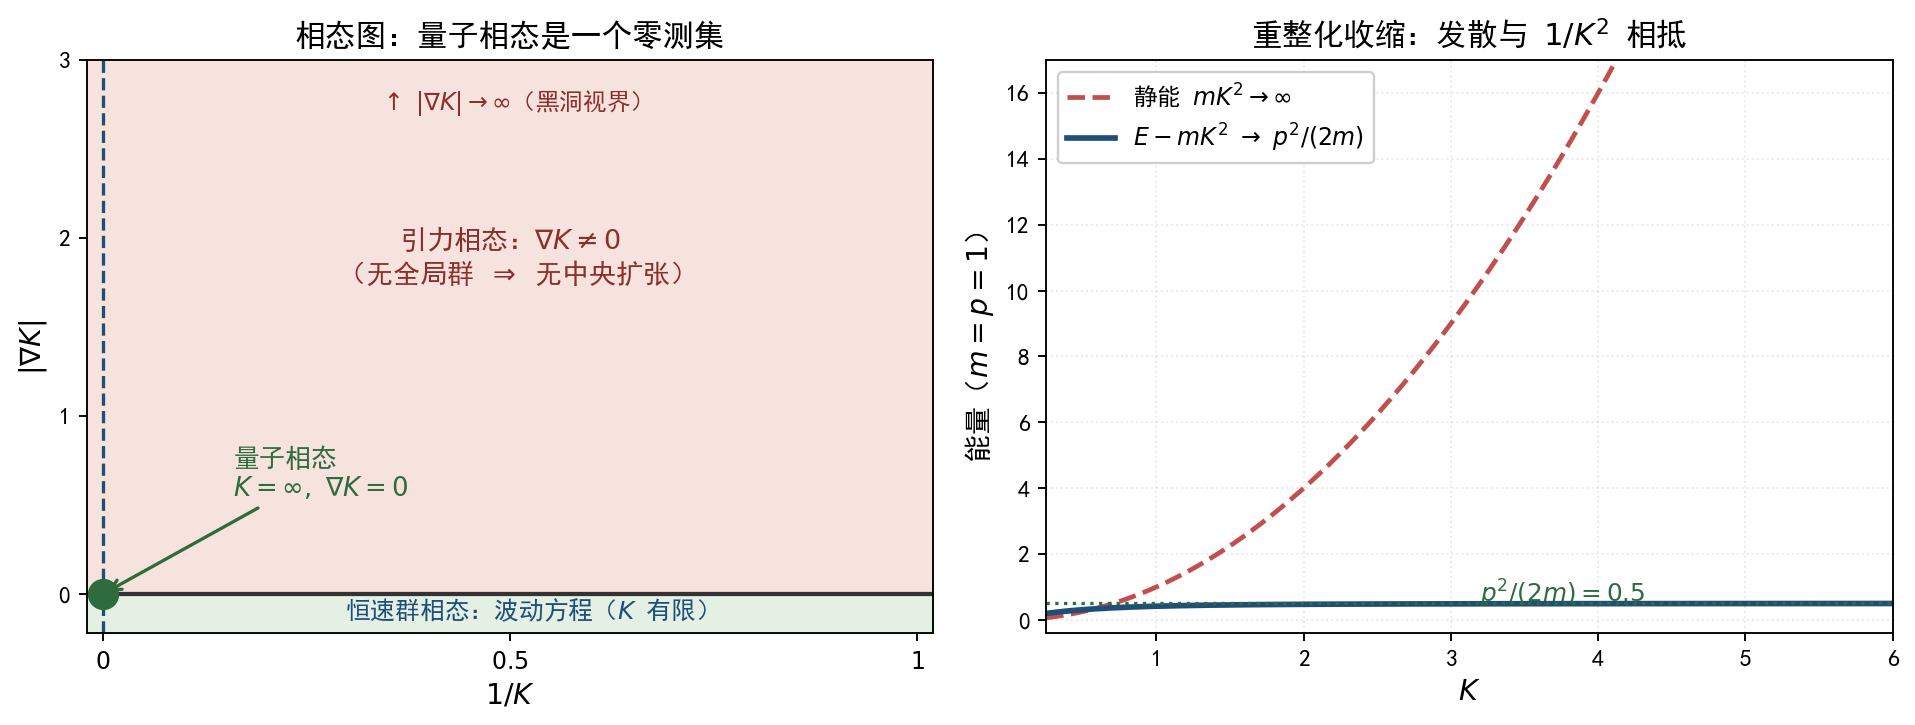
\includegraphics[width=0.88\linewidth,height=\textheight,keepaspectratio]{chapters/images/quantum-phase-boundary.png}

}

\caption{\label{fig-qp-phase}量子相态与引力相态}

\end{figure}%

\section{结论}\label{sec-qp-conclusion}

\begin{longtable}[]{@{}
  >{\raggedright\arraybackslash}p{(\linewidth - 2\tabcolsep) * \real{0.5000}}
  >{\raggedright\arraybackslash}p{(\linewidth - 2\tabcolsep) * \real{0.5000}}@{}}
\caption{本章各命题及其依据}\label{tbl-qp-conclusion}\tabularnewline
\toprule\noalign{}
\begin{minipage}[b]{\linewidth}\raggedright
命题
\end{minipage} & \begin{minipage}[b]{\linewidth}\raggedright
依据
\end{minipage} \\
\midrule\noalign{}
\endfirsthead
\toprule\noalign{}
\begin{minipage}[b]{\linewidth}\raggedright
命题
\end{minipage} & \begin{minipage}[b]{\linewidth}\raggedright
依据
\end{minipage} \\
\midrule\noalign{}
\endhead
\bottomrule\noalign{}
\endlastfoot
\(K\to\infty\) 逐项给出伽利略变换 & 命题~\ref{prp-qp-galileo} \\
不变量退化为 \(\Delta t\) 与 \(\lvert\Delta\mathbf{x}\rvert\) 两个 &
式~\ref{eq-qp-two-invariants} \\
零锥退化为 \(t=\) 常数 & 小节~\ref{sec-qp-part1} \\
恒速代数 \([\hat B_i,\hat P_j]=\frac{i\hbar}{K^{2}}\delta_{ij}\hat H\)
的收缩 & 式~\ref{eq-qp-algK}、定理~\ref{thm-qp-contraction} \\
静能 \(mK^{2}\) 发散与 \(1/K^{2}\) 相抵 ⟹ 中央荷 \(\hat M=m\mathbf 1\) &
定理~\ref{thm-qp-central} \\
经典实现 \(\{K_i,p_j\}=m\delta_{ij}\) 已带中央荷 &
式~\ref{eq-qp-poisson} \\
\(H^{2}(\mathfrak{gal},\mathbb R)=\mathbb R\)，唯一代表元
\(c(\hat B_i,\hat P_j)=\delta_{ij}\) & 定理~\ref{thm-qp-extension} \\
上闭链
\(\xi=\mathbf v_2\cdot R_2\mathbf a_1+\frac12\lvert\mathbf v_2\rvert^{2}b_1\)；Bargmann
群 & 式~\ref{eq-qp-cocycle-explicit} \\
\(m\) 是\textbf{中心元}（非 Casimir 本征值）⟹ 质量超选择 &
定理~\ref{thm-qp-mass} \\
\([\hat q_i,\hat P_j]=i\hbar\delta_{ij}\)；\(\hat M=0\) 时退化为 \(0\) &
定理~\ref{thm-qp-ccr} \\
薛定谔方程的三条独立导出路线 & 式~\ref{eq-qp-schrodinger} \\
静能项严格相消，余项 \(O(K^{-2})\) & 式~\ref{eq-qp-preSch} \\
协变性当且仅当带 \(m\) 相位 & 式~\ref{eq-qp-boost} \\
中央扩张 \(\Longleftrightarrow\vec\nabla K=0\)（Jacobi） &
定理~\ref{thm-qp-jacobi} \\
\(\vec\nabla K\neq0\) ⟹ 残留项 \(\sim K_0^{2}\) 发散 + 反 Hermite &
式~\ref{eq-qp-residual} \\
\end{longtable}

\textbf{一句话}：取定相态参数 \(K\to\infty\)、\(\vec\nabla K=0\)
后，恒速群的李代数经重整化收缩（静能发散与结构常数消失相抵）产生唯一的中央扩张，中央荷即质量
\(m\)；由此解出 \([\hat q_i,\hat P_j]=i\hbar\delta_{ij}\)，并由 Casimir
或德布罗意色散关系生成薛定谔方程；而 Jacobi 恒等式反过来要求
\(\vec\nabla K=0\)------量子力学与引力是两个不相交的相态，二者的强行耦合在本框架内无定义。

\section{术语说明}\label{sec-qp-terms}

{\def\LTcaptype{none} % do not increment counter
\begin{longtable}[]{@{}
  >{\raggedright\arraybackslash}p{(\linewidth - 2\tabcolsep) * \real{0.5000}}
  >{\raggedright\arraybackslash}p{(\linewidth - 2\tabcolsep) * \real{0.5000}}@{}}
\toprule\noalign{}
\begin{minipage}[b]{\linewidth}\raggedright
术语
\end{minipage} & \begin{minipage}[b]{\linewidth}\raggedright
本章中的含义
\end{minipage} \\
\midrule\noalign{}
\endhead
\bottomrule\noalign{}
\endlastfoot
相态参数 & \((K,\vec\nabla K)\)；量子相态为 \((K\to\infty,\,0)\) \\
中央扩张 & 李代数中新增的中心方向；此处唯一，由质量标记 \\
中央荷 \(\hat M\) & 与一切生成元对易的算符；不可约扇区上
\(\hat M=m\mathbf 1\) \\
Casimir 算符 & 由生成元构造、与一切生成元对易的算符；\(K\) 有限时
\(m^{2}\) 是它的本征值 \\
上闭链 / 上边界 & 决定射影表示相位的 \(2\) 形式；模去上边界后即
\(H^{2}\) \\
Bargmann 群 & 伽利略群的中央扩张，多一个中心坐标 \(\zeta\) \\
超选择规则 & 不同中央荷本征值的态不能相干叠加 \\
重整化收缩 & Inönü--Wigner 收缩中先扣除发散部分（此处为静能
\(mK^{2}\)）再取极限 \\
射影表示 & \(U(g_2)U(g_1)=\omega\,U(g_2g_1)\)；由态是射线所致 \\
\end{longtable}
}

\bookmarksetup{startatroot}

\chapter{麦克斯韦方程组}\label{sec-maxwell-equations}

\section{伽利略变换}\label{ux4f3dux5229ux7565ux53d8ux6362-1}

在经典力学中，惯性系~\(S\)~和~\(S'\)（其中~\(S'\)~以恒定速度~\(v\)~沿~\(x\)~轴相对~\(S\)~运动）之间的坐标变换由伽利略变换描述为
式~\ref{eq-galileo}。

\begin{equation}\protect\phantomsection\label{eq-galileo}{
\left\{\begin{aligned}
  & t' = t \\
  & x' = x - vt \\
  & y' = y \\
  & z' = z
 \end{aligned} \right.
}\end{equation}

然而，麦克斯韦方程组预言了真空中光速~\(c\)~为一个普适常数，见
式~\ref{eq-light-speed-c}。

\begin{equation}\protect\phantomsection\label{eq-light-speed-c}{
c = \frac{1}{\sqrt{\mu_{0}\epsilon_{0}}}
}\end{equation}

这与伽利略变换下的速度合成法则相矛盾。

\section{洛伦兹变换}\label{ux6d1bux4f26ux5179ux53d8ux6362-1}

爱因斯坦基于以下两条原理构建了狭义相对论：

\textbf{相对性原理}：所有物理定律在所有惯性参考系中具有相同的形式。

\textbf{光速不变原理}：在任何惯性参考系中，真空中的光速~\(c\)~都相同。

满足这两条原理的坐标变换是洛伦兹变换。采用四维闵可夫斯基时空坐标~\(x^{\nu}=(ct,x,y,z)\)，将时间分量乘以
\(c\)，即取
\(x^{0} = ct\)，是为了让四个分量具有相同的长度量纲，从而变换矩阵的各个元素均为无量纲量。

洛伦兹变换为 式~\ref{eq-lorentz}。

\begin{equation}\protect\phantomsection\label{eq-lorentz}{
\left\{\begin{aligned}
  & t' = \gamma\left(t - \frac{v}{c^{2}}x \right) \\
  & x' = \gamma(x - vt) \\
  & y' = y \\
  & z' = z
 \end{aligned} \right.
}\end{equation}

\begin{equation}\protect\phantomsection\label{eq-beta}{
\beta = \frac{v}{c}
}\end{equation}

\begin{equation}\protect\phantomsection\label{eq-gamma}{
\gamma = \frac{1}{\sqrt{1 - v^{2}/c^{2}}} = \frac{1}{\sqrt{1 - \beta^{2}}}
}\end{equation}

其中 \(\beta\) 为无量纲速度参数，\(\gamma\) 为洛伦兹因子。

设初始时刻~\(S\)~系和~\(S'\)~系的原点重合，\(S'\)~系沿~\(x\)~轴以速度~\(v\)~运动。从
\(S\)~系到~\(S'\)~系的洛伦兹变换的矩阵形式为 式~\ref{eq-lorentz-mat}。

\begin{equation}\protect\phantomsection\label{eq-lorentz-mat}{
x'^{\mu} = \Lambda_{\nu}^{\mu}x^{\nu}
}\end{equation}

其中 式~\ref{eq-lorentz-mat} 中的 \(\Lambda_{\nu}^{\mu}\)
为洛伦兹变换矩阵 式~\ref{eq-Lambda-define}。

\begin{equation}\protect\phantomsection\label{eq-Lambda-define}{
\Lambda_{\nu}^{\mu} = \begin{pmatrix}
\gamma & -\gamma\beta & 0 & 0 \\
-\gamma\beta & \gamma & 0 & 0 \\
0 & 0 & 1 & 0 \\
0 & 0 & 0 & 1
\end{pmatrix}
}\end{equation}

\begin{equation}\protect\phantomsection\label{eq-x-prime}{
x'^{\mu} = \begin{pmatrix}
ct' \\
x' \\
y' \\
z'
\end{pmatrix}
}\end{equation}

\begin{equation}\protect\phantomsection\label{eq-x}{
x^{\nu} = \begin{pmatrix}
ct \\
x \\
y \\
z
\end{pmatrix}
}\end{equation}

将 式~\ref{eq-lorentz-mat} 的矩阵乘法展开，并代入 式~\ref{eq-beta}，得到
式~\ref{eq-t-expand}、式~\ref{eq-x-expand}、式~\ref{eq-y-expand}、式~\ref{eq-z-expand}，合起来就是非矩阵形式的洛伦兹变换
式~\ref{eq-lorentz}。

\begin{equation}\protect\phantomsection\label{eq-t-expand}{
\begin{aligned}
t' &= \frac{1}{c}\left(\gamma(ct) + (-\gamma\beta)x + 0 \cdot y + 0 \cdot z \right) \\
&= \gamma t - \gamma\frac{\beta}{c}x
= \gamma\left(t - \frac{v}{c^{2}}x \right)
\end{aligned}
}\end{equation}

\begin{equation}\protect\phantomsection\label{eq-x-expand}{
\begin{aligned}
x' &= (-\gamma\beta)(ct) + \gamma x + 0 \cdot y + 0 \cdot z \\
&= \gamma x - \gamma\beta ct
= \gamma(x - vt)
\end{aligned}
}\end{equation}

\begin{equation}\protect\phantomsection\label{eq-y-expand}{
y' = 0 \cdot ct + 0 \cdot x + 1 \cdot y + 0 \cdot z = y
}\end{equation}

\begin{equation}\protect\phantomsection\label{eq-z-expand}{
z' = 0 \cdot ct + 0 \cdot x + 0 \cdot y + 1 \cdot z = z
}\end{equation}

从 \(S'\) 系到~\(S\)~系的逆变换，其矩阵形式为
式~\ref{eq-lorentz-inv-mat}，其中 式~\ref{eq-Lambda-inv-define} 中的
\(\Lambda_{\mu}^{\nu}\) 是 式~\ref{eq-Lambda-define} 中
\(\Lambda_{\nu}^{\mu}\) 的逆矩阵。

\begin{equation}\protect\phantomsection\label{eq-lorentz-inv-mat}{
x^{\nu} = \Lambda_{\mu}^{\nu}x'^{\mu}
}\end{equation}

\begin{equation}\protect\phantomsection\label{eq-Lambda-inv-define}{
\Lambda_{\mu}^{\nu} = \begin{pmatrix}
 \gamma & \gamma\beta & 0 & 0 \\
 \gamma\beta & \gamma & 0 & 0 \\
 0 & 0 & 1 & 0 \\
 0 & 0 & 0 & 1
 \end{pmatrix}
}\end{equation}

逆变换的非矩阵形式为 式~\ref{eq-lorentz-inv}。

\begin{equation}\protect\phantomsection\label{eq-lorentz-inv}{
\left\{\begin{aligned}
  & t = \gamma\left(t' + \frac{v}{c^{2}}x' \right) \\
  & x = \gamma\left(x' + vt' \right) \\
  & y = y' \\
  & z = z'
 \end{aligned} \right.
}\end{equation}

\section{麦克斯韦方程组}\label{ux9ea6ux514bux65afux97e6ux65b9ux7a0bux7ec4}

本节将麦克斯韦方程组改写为四维时空中的张量形式\textsuperscript{{[}\citeproc{ref-landaulifshitz1975}{4}{]}}。采用闵可夫斯基度规
\(\eta_{\mu\nu} = \mathrm{diag}(+1,-1,-1,-1)\)；时空指标取
\(\mu,\nu = 0,1,2,3\)，空间指标取
\(i,j = 1,2,3\)，重复的上下指标按爱因斯坦求和约定求和。

\subsection{四维势与电磁场张量}\label{ux56dbux7ef4ux52bfux4e0eux7535ux78c1ux573aux5f20ux91cf}

电磁场张量 \(F^{\mu\nu}\) 由四维势定义为
式~\ref{eq-F-tensor}，它统一了电场和磁场\textsuperscript{{[}\citeproc{ref-jackson1999}{5}{]}}。

\begin{equation}\protect\phantomsection\label{eq-F-tensor}{
F^{\mu\nu} = \partial^{\mu}A^{\nu} - \partial^{\nu}A^{\mu}
}\end{equation}

四维势~\(A^{\mu}\) 为 式~\ref{eq-A-four}，其中
\(\phi\)~是标量势，\(\mathbf{A}\)~是矢量势。

\begin{equation}\protect\phantomsection\label{eq-A-four}{
A^{\mu} = \left(\frac{\phi}{c},\mathbf{A} \right) = \left(\frac{\phi}{c}, A_{x}, A_{y}, A_{z} \right)
}\end{equation}

\(\partial^{\mu}\) 是逆变四维梯度算符，为 式~\ref{eq-partial-four}。

\begin{equation}\protect\phantomsection\label{eq-partial-four}{
\partial^{\mu} = \left(\frac{1}{c}\frac{\partial}{\partial t}, - \boldsymbol{\nabla} \right) = \left(\frac{1}{c}\frac{\partial}{\partial t}, - \frac{\partial}{\partial x}, - \frac{\partial}{\partial y}, - \frac{\partial}{\partial z} \right)
}\end{equation}

电场和磁场\textsuperscript{{[}\citeproc{ref-feynman2020vol2}{6}{]}}（第
240 页）由势定义为 式~\ref{eq-E} 和 式~\ref{eq-B}。

\begin{equation}\protect\phantomsection\label{eq-E}{\mathbf{E} = - \boldsymbol{\nabla}\phi - \frac{\partial\mathbf{A}}{\partial t}}\end{equation}

\begin{equation}\protect\phantomsection\label{eq-B}{
\mathbf{B} = \boldsymbol{\nabla} \times \mathbf{A} =
\begin{vmatrix}
\mathbf{e}_x & \mathbf{e}_y & \mathbf{e}_z \\
\dfrac{\partial}{\partial x} & \dfrac{\partial}{\partial y} & \dfrac{\partial}{\partial z} \\[8pt]
A_x & A_y & A_z
\end{vmatrix}
}\end{equation}

其中 \(\mathbf{e}_x\)、\(\mathbf{e}_y\)、\(\mathbf{e}_z\)
为直角坐标系的单位矢量。式~\ref{eq-E} 的分量形式为
式~\ref{eq-E-i}，式~\ref{eq-B}
的分量形式\textsuperscript{{[}\citeproc{ref-feynman2020vol2}{6}{]}}（第
173 页）为 式~\ref{eq-B-x}、式~\ref{eq-B-y}、式~\ref{eq-B-z}。

\begin{equation}\protect\phantomsection\label{eq-E-i}{ E_{i} = - \frac{\partial\phi}{\partial x^{i}} - \frac{\partial A^i}{\partial t}}\end{equation}

\begin{equation}\protect\phantomsection\label{eq-B-x}{
B_x = (\boldsymbol{\nabla} \times \mathbf{A})_x = \frac{\partial A_z}{\partial y} - \frac{\partial A_y}{\partial z}
}\end{equation}

\begin{equation}\protect\phantomsection\label{eq-B-y}{
B_y = (\boldsymbol{\nabla} \times \mathbf{A})_y = \frac{\partial A_x}{\partial z} - \frac{\partial A_z}{\partial x}
}\end{equation}

\begin{equation}\protect\phantomsection\label{eq-B-z}{
B_z = (\boldsymbol{\nabla} \times \mathbf{A})_z = \frac{\partial A_y}{\partial x} - \frac{\partial A_x}{\partial y}
}\end{equation}

\subsection{计算矩阵形式}\label{ux8ba1ux7b97ux77e9ux9635ux5f62ux5f0f}

根据 式~\ref{eq-F-tensor} 计算 \(F^{\mu\nu}\) 中的上三角元素。

\subsubsection{对角元}\label{ux5bf9ux89d2ux5143}

\(\mu = \nu = i\) 代入 式~\ref{eq-F-tensor} 得到 式~\ref{eq-F-ii}。

\begin{equation}\protect\phantomsection\label{eq-F-ii}{
F^{ii} = \partial^{i}A^i - \partial^{i}A^i = 0
}\end{equation}

\subsubsection{时间-空间分量}\label{ux65f6ux95f4-ux7a7aux95f4ux5206ux91cf}

\(\mu = 0\)，\(\nu = i\) 代入 式~\ref{eq-F-tensor}，化简后代入
式~\ref{eq-E-i} 得到 式~\ref{eq-F-0i}。

\begin{equation}\protect\phantomsection\label{eq-F-0i}{
\begin{aligned}
F^{0i}
&= \partial^{0}A^i - \partial^{i}A^0 \\
&= \frac{1}{c}\frac{\partial A^i}{\partial t}
- \biggl(-\frac{\partial}{\partial x^{i}}\biggr)\biggl(\frac{\phi}{c} \biggr) \\
&= \frac{1}{c}\left(\frac{\partial A^i}{\partial t}
+ \frac{\partial\phi}{\partial x^{i}} \right) \\
&= -\frac{E_{i}}{c}
\end{aligned}
}\end{equation}

\subsubsection{空间-空间分量}\label{ux7a7aux95f4-ux7a7aux95f4ux5206ux91cf}

\(\mu = i,\nu = j\) 代入 式~\ref{eq-F-tensor} 得到 式~\ref{eq-F-ij}，
其中 \(i,j = 1,2,3\)。

\begin{equation}\protect\phantomsection\label{eq-F-ij}{
F^{ij} = \partial^{i}A^j - \partial^{j}A^i= -\frac{\partial A^j}{\partial x^{i}} + \frac{\partial A^i}{\partial x^{j}}
}\end{equation}

计算 \(F^{12}\)，代入 式~\ref{eq-F-ij}，得到 式~\ref{eq-B-field-1}。

\begin{equation}\protect\phantomsection\label{eq-B-field-1}{
F^{12} = -\frac{\partial A^2}{\partial x^{1}} + \frac{\partial A^1}{\partial x^{2}}
 = -\frac{\partial A_{y}}{\partial x} + \frac{\partial A_{x}}{\partial y}
 = -B_z
}\end{equation}

计算 \(F^{13}\)，代入 式~\ref{eq-F-ij}，得到 式~\ref{eq-B-field-2}。

\begin{equation}\protect\phantomsection\label{eq-B-field-2}{
F^{13} = -\frac{\partial A^3}{\partial x^{1}} + \frac{\partial A^1}{\partial x^{3}}
 = -\frac{\partial A_{z}}{\partial x} + \frac{\partial A_{x}}{\partial z}
 = B_y
}\end{equation}

计算 \(F^{23}\)，代入 式~\ref{eq-F-ij}，得到 式~\ref{eq-F-23}。

\begin{equation}\protect\phantomsection\label{eq-F-23}{
F^{23} = -\frac{\partial A^3}{\partial x^{2}} + \frac{\partial A^2}{\partial x^{3}}
 = -\frac{\partial A_{z}}{\partial y} + \frac{\partial A_{y}}{\partial z}
 = -B_x
}\end{equation}

\subsubsection{矩阵形式}\label{ux77e9ux9635ux5f62ux5f0f}

根据 式~\ref{eq-F-tensor} 的定义可知
\(F^{\mu\nu} = - F^{\nu\mu}\)，电磁场张量~\(F^{\mu\nu}\)~是一个反对称二阶张量，下三角各元素可由上三角元素的对称位置加负号得到，其矩阵形式为
式~\ref{eq-F-matrix}。

\begin{equation}\protect\phantomsection\label{eq-F-matrix}{
F^{\mu\nu} = \begin{pmatrix}
0 & - E_x/c & - E_y/c & - E_z/c \\
E_x/c & 0 & -B_z & B_y \\
E_y/c & B_z & 0 & -B_x \\
E_z/c & -B_y & B_x & 0
\end{pmatrix}
}\end{equation}

利用电磁场张量，麦克斯韦方程组可以简洁地表示为两个协变方程：非齐次方程
式~\ref{eq-maxwell-inhomo} 与齐次方程 式~\ref{eq-S-homogeneous}。

\subsection{非齐次麦克斯韦方程组}\label{ux975eux9f50ux6b21ux9ea6ux514bux65afux97e6ux65b9ux7a0bux7ec4}

\begin{equation}\protect\phantomsection\label{eq-maxwell-inhomo}{
\partial_{\mu}F^{\mu\nu} = \mu_{0}J^\nu
}\end{equation}

其中 \(\partial_{\mu}\) 是协变四维导数
式~\ref{eq-partial-cov}，\(J^\nu\)~是四维电流密度
式~\ref{eq-four-current}。

\begin{equation}\protect\phantomsection\label{eq-partial-cov}{
\partial_{\mu} = \left(\frac{1}{c}\frac{\partial}{\partial t},\boldsymbol{\nabla} \right) = \left(\frac{1}{c}\frac{\partial}{\partial t},\frac{\partial}{\partial x},\frac{\partial}{\partial y},\frac{\partial}{\partial z} \right)
}\end{equation}

\begin{equation}\protect\phantomsection\label{eq-four-current}{
J^\nu = (c\rho, \mathbf{J}) = (c\rho, J_x, J_y, J_z)
}\end{equation}

\subsubsection{高斯电场定律}\label{ux9ad8ux65afux7535ux573aux5b9aux5f8b}

取时间分量~\(\nu = 0\)~时，\(\partial_{\mu}F^{\mu 0}\) 是
\(\partial_{\mu}\) 与 \(F^{\mu\nu}\) 第 0 列的点乘，得到
式~\ref{eq-gauss-step1}，其中~\(J^{0} = c\rho\)。

\begin{equation}\protect\phantomsection\label{eq-gauss-step1}{
\frac{\partial}{\partial x}\left(\frac{E_x}{c} \right) + \frac{\partial}{\partial y}\left(\frac{E_y}{c} \right) + \frac{\partial}{\partial z}\left(\frac{E_z}{c} \right) = \mu_{0}c\rho
}\end{equation}

式~\ref{eq-gauss-step1} 两边乘以~\(c\)，得到 式~\ref{eq-gauss-step2}。

\begin{equation}\protect\phantomsection\label{eq-gauss-step2}{
\frac{\partial E_x}{\partial x} + \frac{\partial E_y}{\partial y} + \frac{\partial E_z}{\partial z} = \mu_{0}c^{2}\rho
}\end{equation}

利用 式~\ref{eq-light-speed-c}
得~\(\mu_{0}c^{2} = 1/\epsilon_{0}\)，代入 式~\ref{eq-gauss-step2}
整理后得到高斯电场定律 式~\ref{eq-gauss-E}。

\begin{equation}\protect\phantomsection\label{eq-gauss-E}{
\boldsymbol{\nabla} \cdot \mathbf{E} = \frac{\rho}{\epsilon_{0}}
}\end{equation}

\subsubsection{安培-麦克斯韦定律}\label{ux5b89ux57f9-ux9ea6ux514bux65afux97e6ux5b9aux5f8b}

磁感应强度 \(\mathbf{B}\) 的旋度
\(\boldsymbol{\nabla} \times \mathbf{B}\) 为 式~\ref{eq-nabla-times-B}。

\begin{equation}\protect\phantomsection\label{eq-nabla-times-B}{
\boldsymbol{\nabla} \times \mathbf{B} =
\begin{vmatrix}
\mathbf{e}_x & \mathbf{e}_y & \mathbf{e}_z \\
\frac{\partial}{\partial x} & \frac{\partial}{\partial y} & \frac{\partial}{\partial z} \\
B_x & B_y & B_z
\end{vmatrix}
}\end{equation}

式~\ref{eq-nabla-times-B} 可以展开为三个分量方程
式~\ref{eq-curl-Bx}、式~\ref{eq-curl-By}、式~\ref{eq-curl-Bz}。

\begin{equation}\protect\phantomsection\label{eq-curl-Bx}{
(\boldsymbol{\nabla} \times \mathbf{B})_x = \frac{\partial B_z}{\partial y} - \frac{\partial B_y}{\partial z}
}\end{equation}

\begin{equation}\protect\phantomsection\label{eq-curl-By}{
(\boldsymbol{\nabla} \times \mathbf{B})_y = \frac{\partial B_x}{\partial z} - \frac{\partial B_z}{\partial x}
}\end{equation}

\begin{equation}\protect\phantomsection\label{eq-curl-Bz}{
(\boldsymbol{\nabla} \times \mathbf{B})_z = \frac{\partial B_y}{\partial x} - \frac{\partial B_x}{\partial y}
}\end{equation}

由 式~\ref{eq-light-speed-c} 得到 式~\ref{eq-mu0-eps0}。

\begin{equation}\protect\phantomsection\label{eq-mu0-eps0}{
\frac{1}{c^{2}} = \mu_{0}\epsilon_{0}
}\end{equation}

取空间分量 \(\nu = 1\)~时，\(\partial_{\mu}F^{\mu 1}\) 是
\(\partial_{\mu}\) 与 \(F^{\mu\nu}\) 第 1 列的点乘，得到
式~\ref{eq-amp-m-x}，其中 \(J^{1} = J_{x}\)。

\begin{equation}\protect\phantomsection\label{eq-amp-m-x}{
\frac{1}{c}\frac{\partial}{\partial t}\left(\frac{-E_{x}}{c} \right) + \frac{\partial B_z}{\partial y} - \frac{\partial B_y}{\partial z} = \mu_{0} J_{x}
}\end{equation}

将 式~\ref{eq-mu0-eps0} 和 式~\ref{eq-curl-Bx} 代入 式~\ref{eq-amp-m-x}
后整理得到 式~\ref{eq-amp-x}。

\begin{equation}\protect\phantomsection\label{eq-amp-x}{
\left(\boldsymbol{\nabla} \times \mathbf{B} \right)_{x} - \mu_{0}\epsilon_{0}\frac{\partial E_x}{\partial t} = \mu_{0} J_{x}
}\end{equation}

当~\(\nu = 2\)~时，\(\partial_{\mu}F^{\mu 2}\) 是 \(\partial_{\mu}\) 与
\(F^{\mu\nu}\) 第 2 列的点乘，为 式~\ref{eq-amp-m-y}，其中
\(J^{2} = J_{y}\)。

\begin{equation}\protect\phantomsection\label{eq-amp-m-y}{
\frac{1}{c}\frac{\partial}{\partial t}\left(\frac{-E_{y}}{c} \right) - \frac{\partial B_z}{\partial x} + \frac{\partial B_x}{\partial z} = \mu_{0} J_{y}
}\end{equation}

将 式~\ref{eq-mu0-eps0} 和 式~\ref{eq-curl-By} 代入 式~\ref{eq-amp-m-y}
后整理得到 式~\ref{eq-amp-y}。

\begin{equation}\protect\phantomsection\label{eq-amp-y}{
\left(\boldsymbol{\nabla} \times \mathbf{B} \right)_{y} - \mu_{0}\epsilon_{0}\frac{\partial E_y}{\partial t} = \mu_{0} J_{y}
}\end{equation}

当~\(\nu = 3\)~时，\(\partial_{\mu}F^{\mu 3}\) 是 \(\partial_{\mu}\) 与
\(F^{\mu\nu}\) 第 3 列的点乘，为 式~\ref{eq-amp-m-z}，其中
\(J^{3} = J_{z}\)。

\begin{equation}\protect\phantomsection\label{eq-amp-m-z}{
\frac{1}{c}\frac{\partial}{\partial t}\left(\frac{-E_{z}}{c} \right) + \frac{\partial B_y}{\partial x} - \frac{\partial B_x}{\partial y} = \mu_{0} J_{z}
}\end{equation}

将 式~\ref{eq-mu0-eps0} 和 式~\ref{eq-curl-Bz} 代入 式~\ref{eq-amp-m-z}
后整理得到 式~\ref{eq-amp-z}。

\begin{equation}\protect\phantomsection\label{eq-amp-z}{
\left(\boldsymbol{\nabla} \times \mathbf{B} \right)_{z} - \mu_{0}\epsilon_{0}\frac{\partial E_z}{\partial t} = \mu_{0} J_{z}
}\end{equation}

合并三个分量方程 式~\ref{eq-amp-x}、式~\ref{eq-amp-y}、式~\ref{eq-amp-z}
为矢量形式 式~\ref{eq-ampere}，此方程给出安培-麦克斯韦定律。

\begin{equation}\protect\phantomsection\label{eq-ampere}{
\boldsymbol{\nabla} \times \mathbf{B} = \mu_{0}\mathbf{J} + \mu_{0}\epsilon_{0}\frac{\partial\mathbf{E}}{\partial t}
}\end{equation}

\subsubsection{对应关系}\label{ux5bf9ux5e94ux5173ux7cfb}

表~\ref{tbl-sourceful} 中对 4 维与 3 维的对应关系做了总结：1 个 4
维张量方程包含了 2 个 3 维矢量方程。

\begin{longtable}[]{@{}
  >{\raggedright\arraybackslash}p{(\linewidth - 4\tabcolsep) * \real{0.3400}}
  >{\raggedright\arraybackslash}p{(\linewidth - 4\tabcolsep) * \real{0.3800}}
  >{\raggedright\arraybackslash}p{(\linewidth - 4\tabcolsep) * \real{0.2800}}@{}}
\caption{有源项：4 维与 3
维的对应关系}\label{tbl-sourceful}\tabularnewline
\toprule\noalign{}
\begin{minipage}[b]{\linewidth}\raggedright
4 维形式
\end{minipage} & \begin{minipage}[b]{\linewidth}\raggedright
3 维形式
\end{minipage} & \begin{minipage}[b]{\linewidth}\raggedright
物理定律
\end{minipage} \\
\midrule\noalign{}
\endfirsthead
\toprule\noalign{}
\begin{minipage}[b]{\linewidth}\raggedright
4 维形式
\end{minipage} & \begin{minipage}[b]{\linewidth}\raggedright
3 维形式
\end{minipage} & \begin{minipage}[b]{\linewidth}\raggedright
物理定律
\end{minipage} \\
\midrule\noalign{}
\endhead
\bottomrule\noalign{}
\endlastfoot
\(\partial_\mu F^{\mu\nu} = \mu_0 J^\nu\)，\(\nu = 0\) &
\(\boldsymbol{\nabla} \cdot \mathbf{E} = \rho/\epsilon_0\) &
高斯电场定律 \\
\(\partial_\mu F^{\mu\nu} = \mu_0 J^\nu\)，\(\nu = 1,2,3\) &
\(\boldsymbol{\nabla} \times \mathbf{B} = \mu_0 \mathbf{J} + \mu_0 \epsilon_0 \partial_t \mathbf{E}\)
& 安培-麦克斯韦定律 \\
\end{longtable}

时间分量（\(\nu = 0\)）对应高斯电场定律，空间分量（\(\nu = 1,2,3\)）对应安培-麦克斯韦定律。

\subsection{齐次麦克斯韦方程组}\label{ux9f50ux6b21ux9ea6ux514bux65afux97e6ux65b9ux7a0bux7ec4}

循环（指标三重交替）形式为 式~\ref{eq-S-homogeneous}，该式对指标
\(\lambda,\mu,\nu\) 的任意取值均成立。

\begin{equation}\protect\phantomsection\label{eq-S-homogeneous}{
\partial^{\lambda}F^{\mu\nu} + \partial^{\mu}F^{\nu\lambda} + \partial^{\nu}F^{\lambda\mu} = 0
}\end{equation}

\subsubsection{高斯磁场定律}\label{ux9ad8ux65afux78c1ux573aux5b9aux5f8b}

式~\ref{eq-S-homogeneous} 选择 \((\lambda,\mu,\nu) = (1,2,3)\) 得到
式~\ref{eq-hom-123}。

\begin{equation}\protect\phantomsection\label{eq-hom-123}{
\partial^{1}F^{23} + \partial^{2}F^{31} + \partial^{3}F^{12} = 0
}\end{equation}

将 式~\ref{eq-partial-four} 和 式~\ref{eq-F-matrix} 代入
式~\ref{eq-hom-123}，得到 式~\ref{eq-hom-123-sub}。

\begin{equation}\protect\phantomsection\label{eq-hom-123-sub}{
- \frac{\partial}{\partial x}\left(- B_x \right) - \frac{\partial}{\partial y}\left(- B_y \right) - \frac{\partial}{\partial z}\left(- B_z \right) = 0
}\end{equation}

将 式~\ref{eq-hom-123-sub} 整理后得高斯磁场定律 式~\ref{eq-gauss-B}。

\begin{equation}\protect\phantomsection\label{eq-gauss-B}{
\boldsymbol{\nabla} \cdot \mathbf{B} = 0
}\end{equation}

\subsubsection{法拉第电磁感应定律}\label{ux6cd5ux62c9ux7b2cux7535ux78c1ux611fux5e94ux5b9aux5f8b}

电场 \(\mathbf{E}\) 的旋度 \(\boldsymbol{\nabla} \times \mathbf{E}\) 为
式~\ref{eq-nabla-times-E}。

\begin{equation}\protect\phantomsection\label{eq-nabla-times-E}{
\boldsymbol{\nabla} \times \mathbf{E} =
\begin{vmatrix}
\mathbf{e}_x & \mathbf{e}_y & \mathbf{e}_z \\
\frac{\partial}{\partial x} & \frac{\partial}{\partial y} & \frac{\partial}{\partial z} \\
E_x & E_y & E_z
\end{vmatrix}
}\end{equation}

式~\ref{eq-nabla-times-E} 可以展开为三个分量方程
式~\ref{eq-curl-Ex}、式~\ref{eq-curl-Ey}、式~\ref{eq-curl-Ez}。

\begin{equation}\protect\phantomsection\label{eq-curl-Ex}{
(\boldsymbol{\nabla} \times \mathbf{E})_x = \frac{\partial E_z}{\partial y} - \frac{\partial E_y}{\partial z}
}\end{equation}

\begin{equation}\protect\phantomsection\label{eq-curl-Ey}{
(\boldsymbol{\nabla} \times \mathbf{E})_y = \frac{\partial E_x}{\partial z} - \frac{\partial E_z}{\partial x}
}\end{equation}

\begin{equation}\protect\phantomsection\label{eq-curl-Ez}{
(\boldsymbol{\nabla} \times \mathbf{E})_z = \frac{\partial E_y}{\partial x} - \frac{\partial E_x}{\partial y}
}\end{equation}

x-分量：式~\ref{eq-S-homogeneous} 选择
\((\lambda,\mu,\nu) = (0,2,3)\)，得到 式~\ref{eq-hom-023}。

\begin{equation}\protect\phantomsection\label{eq-hom-023}{
\partial^{0}F^{23} + \partial^{2}F^{30} + \partial^{3}F^{02} = 0
}\end{equation}

将 式~\ref{eq-partial-four} 和 式~\ref{eq-F-matrix} 代入
式~\ref{eq-hom-023} 得到 式~\ref{eq-hom-023-sub}。

\begin{equation}\protect\phantomsection\label{eq-hom-023-sub}{
\frac{1}{c}\frac{\partial}{\partial t}\left(- B_x \right) - \frac{\partial}{\partial y}\left(\frac{E_z}{c} \right) - \frac{\partial}{\partial z}\left(- \frac{E_y}{c} \right) = 0
}\end{equation}

将 式~\ref{eq-hom-023-sub} 乘 \(c\) 整理后得到
式~\ref{eq-m-nabla-times-E-x}。

\begin{equation}\protect\phantomsection\label{eq-m-nabla-times-E-x}{
- \frac{\partial B_x}{\partial t} - \frac{\partial E_z}{\partial y} + \frac{\partial E_y}{\partial z} = 0
}\end{equation}

将 式~\ref{eq-curl-Ex} 代入 式~\ref{eq-m-nabla-times-E-x} 得到
式~\ref{eq-nabla-times-E-x}。

\begin{equation}\protect\phantomsection\label{eq-nabla-times-E-x}{
\left(\boldsymbol{\nabla} \times \mathbf{E} \right)_{x} = -\frac{\partial B_x}{\partial t}
}\end{equation}

y-分量：式~\ref{eq-S-homogeneous} 选择
\((\lambda,\mu,\nu) = (0,3,1)\)，得到 式~\ref{eq-hom-031}。

\begin{equation}\protect\phantomsection\label{eq-hom-031}{
\partial^{0}F^{31} + \partial^{3}F^{10} + \partial^{1}F^{03} = 0
}\end{equation}

将 式~\ref{eq-partial-four} 和 式~\ref{eq-F-matrix} 代入
式~\ref{eq-hom-031} 得到 式~\ref{eq-hom-031-sub}。

\begin{equation}\protect\phantomsection\label{eq-hom-031-sub}{
\frac{1}{c}\frac{\partial}{\partial t}\left(- B_y \right) - \frac{\partial}{\partial z}\left(\frac{E_x}{c} \right) - \frac{\partial}{\partial x}\left(- \frac{E_z}{c} \right) = 0
}\end{equation}

将 式~\ref{eq-hom-031-sub} 乘 \(c\) 整理后得到
式~\ref{eq-m-nabla-times-E-y}。

\begin{equation}\protect\phantomsection\label{eq-m-nabla-times-E-y}{
- \frac{\partial B_y}{\partial t} - \frac{\partial E_x}{\partial z} + \frac{\partial E_z}{\partial x} = 0
}\end{equation}

将 式~\ref{eq-curl-Ey} 代入 式~\ref{eq-m-nabla-times-E-y} 得到
式~\ref{eq-nabla-times-E-y}。

\begin{equation}\protect\phantomsection\label{eq-nabla-times-E-y}{
\left(\boldsymbol{\nabla} \times \mathbf{E} \right)_{y} = -\frac{\partial B_y}{\partial t}
}\end{equation}

z-分量：式~\ref{eq-S-homogeneous} 选择
\((\lambda,\mu,\nu) = (0,1,2)\)，得到 式~\ref{eq-hom-012}。

\begin{equation}\protect\phantomsection\label{eq-hom-012}{
\partial^{0}F^{12} + \partial^{1}F^{20} + \partial^{2}F^{01} = 0
}\end{equation}

将 式~\ref{eq-partial-four} 和 式~\ref{eq-F-matrix} 代入
式~\ref{eq-hom-012} 得到 式~\ref{eq-hom-012-sub}。

\begin{equation}\protect\phantomsection\label{eq-hom-012-sub}{
\frac{1}{c}\frac{\partial}{\partial t}\left(- B_z \right) - \frac{\partial}{\partial x}\left(\frac{E_y}{c} \right) - \frac{\partial}{\partial y}\left(- \frac{E_x}{c} \right) = 0
}\end{equation}

将 式~\ref{eq-hom-012-sub} 乘 \(c\) 整理后得到
式~\ref{eq-m-nabla-times-E-z}。

\begin{equation}\protect\phantomsection\label{eq-m-nabla-times-E-z}{
- \frac{\partial B_z}{\partial t} - \frac{\partial E_y}{\partial x} + \frac{\partial E_x}{\partial y} = 0
}\end{equation}

将 式~\ref{eq-curl-Ez} 代入 式~\ref{eq-m-nabla-times-E-z} 得到
式~\ref{eq-nabla-times-E-z}。

\begin{equation}\protect\phantomsection\label{eq-nabla-times-E-z}{
\left(\boldsymbol{\nabla} \times \mathbf{E} \right)_{z} = -\frac{\partial B_z}{\partial t}
}\end{equation}

合并三个分量方程
式~\ref{eq-nabla-times-E-x}、式~\ref{eq-nabla-times-E-y}、式~\ref{eq-nabla-times-E-z}
得到法拉第电磁感应定律 式~\ref{eq-farad}。

\begin{equation}\protect\phantomsection\label{eq-farad}{\boldsymbol{\nabla} \times \mathbf{E} = -\frac{\partial\mathbf{B}}{\partial t}}\end{equation}

\subsubsection{对应关系}\label{ux5bf9ux5e94ux5173ux7cfb-1}

表~\ref{tbl-sourceless} 中对 4 维与 3 维的对应关系做了总结：1 个 4
维张量方程包含了 2 个 3 维矢量方程。

\begin{longtable}[]{@{}
  >{\raggedright\arraybackslash}p{(\linewidth - 4\tabcolsep) * \real{0.5700}}
  >{\raggedright\arraybackslash}p{(\linewidth - 4\tabcolsep) * \real{0.1800}}
  >{\raggedright\arraybackslash}p{(\linewidth - 4\tabcolsep) * \real{0.2500}}@{}}
\caption{无源项：4 维与 3
维的对应关系}\label{tbl-sourceless}\tabularnewline
\toprule\noalign{}
\begin{minipage}[b]{\linewidth}\raggedright
4 维形式
\end{minipage} & \begin{minipage}[b]{\linewidth}\raggedright
3 维形式
\end{minipage} & \begin{minipage}[b]{\linewidth}\raggedright
物理定律
\end{minipage} \\
\midrule\noalign{}
\endfirsthead
\toprule\noalign{}
\begin{minipage}[b]{\linewidth}\raggedright
4 维形式
\end{minipage} & \begin{minipage}[b]{\linewidth}\raggedright
3 维形式
\end{minipage} & \begin{minipage}[b]{\linewidth}\raggedright
物理定律
\end{minipage} \\
\midrule\noalign{}
\endhead
\bottomrule\noalign{}
\endlastfoot
\(\partial^{\lambda}F^{\mu\nu}+\partial^{\mu}F^{\nu\lambda}+\partial^{\nu}F^{\lambda\mu} = 0\)，\((\lambda,\mu,\nu)=(1,2,3)\)
& \(\boldsymbol{\nabla} \cdot \mathbf{B} = 0\) & 高斯磁场定律 \\
\(\partial^{\lambda}F^{\mu\nu}+\partial^{\mu}F^{\nu\lambda}+\partial^{\nu}F^{\lambda\mu} = 0\)，\((\lambda,\mu,\nu)\in\{(0,2,3),(0,3,1),(0,1,2)\}\)
&
\(\boldsymbol{\nabla} \times \mathbf{E} = -\frac{\partial\mathbf{B}}{\partial t}\)
& 法拉第电磁感应定律 \\
\end{longtable}

\section{协变性与电磁场的变换}\label{ux534fux53d8ux6027ux4e0eux7535ux78c1ux573aux7684ux53d8ux6362}

本节证明麦克斯韦方程组在洛伦兹变换下是协变的：若方程组在惯性系 \(S\)
中成立，则在洛伦兹变换后的惯性系 \(S'\)
中具有相同的形式。其中非齐次方程协变性的证明，核心是证明
式~\ref{eq-cov-final}；齐次方程的形式不变性由 式~\ref{eq-S-homogeneous}
的循环结构保证；最后由张量变换法则导出电场与磁场分量的显式变换关系。

\subsection{物理量的洛伦兹变换}\label{ux7269ux7406ux91cfux7684ux6d1bux4f26ux5179ux53d8ux6362}

在洛伦兹变换下，各物理量按其张量阶数以确定的规则变换。四维矢量按
式~\ref{eq-A-transform} 变换，其中 \(\Lambda_{\nu}^{\mu}\) 为
式~\ref{eq-Lambda-define}。

\begin{equation}\protect\phantomsection\label{eq-A-transform}{
A'^{\nu} = \Lambda_{\sigma}^{\nu}A^{\sigma}
}\end{equation}

偏导数算符的变换由链式法则导出。对 式~\ref{eq-lorentz-mat} 求逆得
式~\ref{eq-lorentz-inv-mat}，于是
\(\partial'_{\mu} = \frac{\partial x^{\nu}}{\partial x'^{\mu}}\partial_{\nu} = \Lambda_{\mu}^{\nu}\partial_{\nu}\)，即协变四维导数的变换
式~\ref{eq-partial-cov-transform}；用度规升指标后，逆变四维导数的变换为
式~\ref{eq-part-mu}。

\begin{equation}\protect\phantomsection\label{eq-partial-cov-transform}{
\partial'_{\mu} = \Lambda_{\mu}^{\nu}\partial_{\nu}
}\end{equation}

\begin{equation}\protect\phantomsection\label{eq-part-mu}{
\partial'^{\mu} = \Lambda_{\rho}^{\mu}\partial^{\rho}
}\end{equation}

在~\(S'\)~系中，电磁场张量定义为 式~\ref{eq-F-prime-def}。

\begin{equation}\protect\phantomsection\label{eq-F-prime-def}{
F'^{\mu\nu} = \partial'^{\mu}A'^{\nu} - \partial'^{\nu}A'^{\mu}
}\end{equation}

将 式~\ref{eq-A-transform} 和 式~\ref{eq-part-mu} 代入
式~\ref{eq-F-prime-def}。由于洛伦兹变换矩阵的元素是常数，可以提到偏导算符之前；又因矩阵元素是普通实数，乘法可交换，\(\Lambda_{\rho}^{\mu}\Lambda_{\sigma}^{\nu} = \Lambda_{\sigma}^{\nu}\Lambda_{\rho}^{\mu}\)，于是得到
式~\ref{eq-F-formula-to-mu-nu}。

\begin{equation}\protect\phantomsection\label{eq-F-formula-to-mu-nu}{
\begin{aligned}
F'^{\mu\nu}
&= \left(\Lambda_{\rho}^{\mu}\partial^{\rho} \right)\left(\Lambda_{\sigma}^{\nu}A^{\sigma} \right)
- \left(\Lambda_{\sigma}^{\nu}\partial^{\sigma} \right)\left(\Lambda_{\rho}^{\mu}A^{\rho} \right) \\
&= \Lambda_{\rho}^{\mu}\Lambda_{\sigma}^{\nu}\partial^{\rho}A^{\sigma}
- \Lambda_{\rho}^{\mu}\Lambda_{\sigma}^{\nu}\partial^{\sigma}A^{\rho} \\
&= \left(\Lambda_{\rho}^{\mu}\Lambda_{\sigma}^{\nu} \right)
\bigl(\partial^{\rho}A^{\sigma} - \partial^{\sigma}A^{\rho} \bigr) \\
&= \Lambda_{\rho}^{\mu}\Lambda_{\sigma}^{\nu}F^{\rho\sigma}
\end{aligned}
}\end{equation}

最后，根据 式~\ref{eq-F-tensor} 的定义，得到电磁场张量的变换法则
式~\ref{eq-F-to-formula}。

\begin{equation}\protect\phantomsection\label{eq-F-to-formula}{
F'^{\mu\nu} = \Lambda_{\rho}^{\mu}\Lambda_{\sigma}^{\nu}F^{\rho\sigma}
}\end{equation}

同理，四维电流密度与协变四维导数分别按 式~\ref{eq-J-transform} 和
式~\ref{eq-partial-cov-transform} 变换。

\begin{equation}\protect\phantomsection\label{eq-J-transform}{
J'^{\mu} = \Lambda_{\nu}^{\mu}J^{\nu}
}\end{equation}

\subsection{非齐次方程的协变性}\label{ux975eux9f50ux6b21ux65b9ux7a0bux7684ux534fux53d8ux6027}

将 式~\ref{eq-F-to-formula} 和 式~\ref{eq-partial-cov-transform} 代入
\(\partial'_{\mu}F'^{\mu\nu}\)。为避免哑指标与自由指标重复，将求和指标改记为
\(\alpha\)；由于 \(\Lambda\) 的元素是常数，可提到偏导算符之前，得到
式~\ref{eq-cov-step1}。

\begin{equation}\protect\phantomsection\label{eq-cov-step1}{
\begin{aligned}
\partial'_{\mu}F'^{\mu\nu}
&= \left(\Lambda_{\mu}^{\alpha}\partial_{\alpha} \right)
\left(\Lambda_{\rho}^{\mu}\Lambda_{\sigma}^{\nu}F^{\rho\sigma} \right) \\
&= \Lambda_{\mu}^{\alpha}\Lambda_{\rho}^{\mu}\Lambda_{\sigma}^{\nu}\partial_{\alpha}F^{\rho\sigma}
\end{aligned}
}\end{equation}

洛伦兹变换矩阵满足正交关系 式~\ref{eq-cov-orthogonal}（即
\(\Lambda^{-1}\Lambda = I\)）。

\begin{equation}\protect\phantomsection\label{eq-cov-orthogonal}{
\Lambda_{\mu}^{\alpha}\Lambda_{\rho}^{\mu} = \delta_{\rho}^{\alpha}
}\end{equation}

其中 Kronecker 符号 \(\delta_{\rho}^{\alpha}\) 在 \(\rho = \alpha\) 时为
1，否则为 0。利用 式~\ref{eq-cov-orthogonal} 化简
式~\ref{eq-cov-step1}，得到 式~\ref{eq-cov-step2}。

\begin{equation}\protect\phantomsection\label{eq-cov-step2}{
\partial'_{\mu}F'^{\mu\nu} = \Lambda_{\sigma}^{\nu}\partial_{\rho}F^{\rho\sigma}
}\end{equation}

在~\(S\)~系中 式~\ref{eq-maxwell-inhomo}
成立，即~\(\partial_{\rho}F^{\rho\sigma} = \mu_{0}J^{\sigma}\)，代入
式~\ref{eq-cov-step2} 得到 式~\ref{eq-cov-step3}。

\begin{equation}\protect\phantomsection\label{eq-cov-step3}{
\partial'_{\mu}F'^{\mu\nu} = \Lambda_{\sigma}^{\nu}\mu_{0}J^{\sigma} = \mu_{0}\Lambda_{\sigma}^{\nu}J^{\sigma}
}\end{equation}

根据四维电流密度的变换
式~\ref{eq-J-transform}，\(\Lambda_{\sigma}^{\nu}J^{\sigma} = J'^{\nu}\)，于是得到
式~\ref{eq-cov-final}。

\begin{equation}\protect\phantomsection\label{eq-cov-final}{
\partial'_{\mu}F'^{\mu\nu} = \mu_{0}J'^{\nu}
}\end{equation}

式~\ref{eq-cov-final} 与 式~\ref{eq-maxwell-inhomo}
具有相同的形式，这证明了非齐次麦克斯韦方程组在洛伦兹变换下是协变的。

\subsection{齐次方程的协变性}\label{ux9f50ux6b21ux65b9ux7a0bux7684ux534fux53d8ux6027}

证明循环形式的齐次方程 式~\ref{eq-S-homogeneous}
在洛伦兹变换下形式不变，即：如果在参考系 \(S\) 中
式~\ref{eq-S-homogeneous} 成立，则在参考系 \(S'\) 中，相应的
式~\ref{eq-S-2-homogeneous} 也成立。

\begin{equation}\protect\phantomsection\label{eq-S-2-homogeneous}{
\partial'^{\lambda}F'^{\mu\nu} + \partial'^{\mu}F'^{\nu\lambda} + \partial'^{\nu}F'^{\lambda\mu} = 0
}\end{equation}

将变换规则 式~\ref{eq-part-mu} 和 式~\ref{eq-F-to-formula} 代入
式~\ref{eq-S-2-homogeneous} 的第一项，得到 式~\ref{eq-hom-cov-term1}。

\begin{equation}\protect\phantomsection\label{eq-hom-cov-term1}{
\partial'^{\lambda}F'^{\mu\nu} = \left(\Lambda_{\rho}^{\lambda}\partial^{\rho} \right)\left(\Lambda_{\alpha}^{\mu}\Lambda_{\beta}^{\nu}F^{\alpha\beta} \right)
= \Lambda_{\rho}^{\lambda} \Lambda_{\alpha}^{\mu}\Lambda_{\beta}^{\nu}\partial^{\rho}F^{\alpha\beta}
}\end{equation}

同理，式~\ref{eq-S-2-homogeneous} 的第二项得到
式~\ref{eq-hom-cov-term2}，第三项得到 式~\ref{eq-hom-cov-term3}。

\begin{equation}\protect\phantomsection\label{eq-hom-cov-term2}{
\partial'^{\mu}F'^{\nu\lambda} = \Lambda_{\alpha}^{\mu} \Lambda_{\beta}^{\nu}\Lambda_{\rho}^{\lambda}\partial^{\alpha}F^{\beta\rho}
}\end{equation}

\begin{equation}\protect\phantomsection\label{eq-hom-cov-term3}{
\partial'^{\nu}F'^{\lambda\mu} = \Lambda_{\beta}^{\nu} \Lambda_{\rho}^{\lambda}\Lambda_{\alpha}^{\mu}\partial^{\beta}F^{\rho\alpha}
}\end{equation}

式~\ref{eq-S-2-homogeneous} 变换后的方程左端变为
式~\ref{eq-hom-cov-sum}。

\begin{equation}\protect\phantomsection\label{eq-hom-cov-sum}{
\begin{aligned}
& \Lambda_{\rho}^{\lambda} \Lambda_{\alpha}^{\mu} \Lambda_{\beta}^{\nu}\, \partial^{\rho}F^{\alpha\beta} + \Lambda_{\alpha}^{\mu} \Lambda_{\beta}^{\nu} \Lambda_{\rho}^{\lambda}\, \partial^{\alpha}F^{\beta\rho} + \Lambda_{\beta}^{\nu} \Lambda_{\rho}^{\lambda} \Lambda_{\alpha}^{\mu}\, \partial^{\beta}F^{\rho\alpha} \\
=& \Lambda_{\rho}^{\lambda} \Lambda_{\alpha}^{\mu} \Lambda_{\beta}^{\nu}
\biggl(\partial^{\rho}F^{\alpha\beta}
+ \partial^{\alpha}F^{\beta\rho}
+ \partial^{\beta}F^{\rho\alpha} \biggr) = 0
\end{aligned}
}\end{equation}

由于 \(\Lambda_{\nu}^{\mu}\)
是数字（矩阵元素），数的乘法可交换，因此可以将每个乘积中的因子重新排序：三个乘积实际上包含相同的因子
\(\Lambda_{\rho}^{\lambda} \Lambda_{\alpha}^{\mu}\Lambda_{\beta}^{\nu}\)，只是顺序不同。而括号内正是
\(S\) 系中的齐次方程 式~\ref{eq-S-homogeneous}（将指标
\((\lambda,\mu,\nu)\) 换为 \((\rho,\alpha,\beta)\)），故其值为
0。这就证明了 式~\ref{eq-S-2-homogeneous} 成立。

\subsection{电磁场的变换关系}\label{ux7535ux78c1ux573aux7684ux53d8ux6362ux5173ux7cfb}

在 \(S'\) 系中，\(F'^{\mu\nu}\) 同样由该系的四维势 \(A'^{\mu}\) 按
式~\ref{eq-F-prime-def} 的方式定义，因而也是反对称张量，其矩阵元素与
\(\mathbf{E}'\)、\(\mathbf{B}'\) 的对应关系和 \(S\) 系中一致，即
式~\ref{eq-F-mat-to-mu-nu} 中的 \(F'^{\mu\nu}\) 与 式~\ref{eq-F-matrix}
中的 \(F^{\mu\nu}\) 具有相同的形式。

\begin{equation}\protect\phantomsection\label{eq-F-mat-to-mu-nu}{
F'^{\mu\nu} = \begin{pmatrix}
 0 & - E'_x/c & - E'_y/c & - E'_z/c \\
 E'_x/c & 0 & - B'_z & B'_y \\
 E'_y/c & B'_z & 0 & -B'_{x} \\
 E'_z/c & - B'_y & B'_x & 0
 \end{pmatrix}
}\end{equation}

根据电磁场张量的变换法则
式~\ref{eq-F-to-formula}，可以推导出三维空间中电场和磁场分量的显式变换关系\textsuperscript{{[}\citeproc{ref-griffiths2025}{7}{]}}。

\subsubsection{\texorpdfstring{\(E'_x\) 与
\(F'^{01}\)~分量}{E\textquotesingle\_x 与 F\textquotesingle\^{}\{01\}~分量}}\label{e_x-ux4e0e-f01-ux5206ux91cf}

式~\ref{eq-F-to-formula} 中取 \(\mu = 0\)，\(\nu = 1\)，得到
式~\ref{eq-m-F-to-01}。

\begin{equation}\protect\phantomsection\label{eq-m-F-to-01}{
F'^{01} = \Lambda_{\rho}^{0}\Lambda_{\sigma}^{1}F^{\rho\sigma}
= \sum_{\rho = 0}^{3}\sum_{\sigma = 0}^{3}\Lambda_{\rho}^{0}\Lambda_{\sigma}^{1}F^{\rho\sigma}
}\end{equation}

根据 式~\ref{eq-gamma} 得到 式~\ref{eq-gamma-beta}。

\begin{equation}\protect\phantomsection\label{eq-gamma-beta}{
\gamma^{2}\left(1 - \beta^{2} \right) = 1
}\end{equation}

将 式~\ref{eq-Lambda-define}、式~\ref{eq-F-matrix} 和
式~\ref{eq-gamma-beta} 代入 式~\ref{eq-m-F-to-01}，只保留非零元素，得到
式~\ref{eq-F-to-01}。

\begin{equation}\protect\phantomsection\label{eq-F-to-01}{
\begin{aligned}
-\frac{E'_x}{c}
&= \Lambda_{0}^{0}\Lambda_{1}^{1}\,F^{01}
+ \Lambda_{1}^{0}\Lambda_{0}^{1}\,F^{10} \\
&= \gamma\gamma\left(-\frac{E_x}{c}\right)
+ (-\gamma\beta)(-\gamma\beta)\left(\frac{E_x}{c}\right) \\
&= \gamma^{2}\bigl(1-\beta^{2}\bigr)\left(-\frac{E_x}{c}\right) \\
&= -\frac{E_x}{c}
\end{aligned}
}\end{equation}

式~\ref{eq-F-to-01} 两边同乘以 \(-c\)，得到 式~\ref{eq-E-to-x}。

\subsubsection{\texorpdfstring{\(E'_y\) 与 \(F'^{02}\)
分量}{E\textquotesingle\_y 与 F\textquotesingle\^{}\{02\} 分量}}\label{e_y-ux4e0e-f02-ux5206ux91cf}

式~\ref{eq-F-to-formula} 中取 \(\mu = 0\)，\(\nu = 2\)。由于
\(\Lambda_{\sigma}^{2}\) 只有在~\(\sigma = 2\)~时为 1，其它为 0，得到
式~\ref{eq-m-F-to-02}。

\begin{equation}\protect\phantomsection\label{eq-m-F-to-02}{
F'^{02} = \Lambda_{\rho}^{0}\Lambda_{\sigma}^{2}F^{\rho\sigma}
= \sum_{\rho = 0}^{3}\Lambda_{\rho}^{0}F^{\rho 2}
}\end{equation}

将 式~\ref{eq-Lambda-define} 和 式~\ref{eq-F-matrix} 代入
式~\ref{eq-m-F-to-02}，只保留非零元素，得到 式~\ref{eq-F-to-02}。

\begin{equation}\protect\phantomsection\label{eq-F-to-02}{
\begin{aligned}
-\frac{E'_y}{c} &= \Lambda_{0}^{0} F^{02} + \Lambda_{1}^{0} F^{12} \\
 &= \gamma \cdot \left(-\frac{E_y}{c} \right) + (-\gamma\beta) \cdot (- B_z ) \\
 &= \gamma \left(- \frac{E_y}{c} + \beta B_z \right)
\end{aligned}
}\end{equation}

式~\ref{eq-F-to-02} 两边同乘以 \(-c\)，并代入 式~\ref{eq-beta}，得到
式~\ref{eq-E-to-y}。

\subsubsection{\texorpdfstring{\(E'_z\) 与
\(F'^{03}\)~分量}{E\textquotesingle\_z 与 F\textquotesingle\^{}\{03\}~分量}}\label{e_z-ux4e0e-f03-ux5206ux91cf}

式~\ref{eq-F-to-formula} 中取 \(\mu = 0\)，\(\nu = 3\)。由于
\(\Lambda_{\sigma}^{3}\) 只有在~\(\sigma = 3\)~时为 1，其它为 0，得到
式~\ref{eq-m-F-to-03}。

\begin{equation}\protect\phantomsection\label{eq-m-F-to-03}{
F'^{03} = \Lambda_{\rho}^{0}\Lambda_{\sigma}^{3}F^{\rho\sigma}
= \sum_{\rho = 0}^{3}\Lambda_{\rho}^{0}F^{\rho 3}
}\end{equation}

将 式~\ref{eq-Lambda-define} 和 式~\ref{eq-F-matrix} 代入
式~\ref{eq-m-F-to-03}，只保留非零元素，得到 式~\ref{eq-F-to-03}。

\begin{equation}\protect\phantomsection\label{eq-F-to-03}{
\begin{aligned}
-\frac{E'_z}{c}
&= \Lambda_{0}^{0}\,F^{03} + \Lambda_{1}^{0}\,F^{13} \\
&= \gamma\left(-\frac{E_z}{c}\right) + (-\gamma\beta) B_y \\
&= \gamma\left(-\frac{E_z}{c} - \beta B_y \right)
\end{aligned}
}\end{equation}

式~\ref{eq-F-to-03} 两边同乘以 \(-c\)，并代入 式~\ref{eq-beta}，得到
式~\ref{eq-E-to-z}。

\subsubsection{\texorpdfstring{\(B'_x\) 与
\(F'^{23}\)~分量}{B\textquotesingle\_x 与 F\textquotesingle\^{}\{23\}~分量}}\label{b_x-ux4e0e-f23-ux5206ux91cf}

式~\ref{eq-F-to-formula} 中取 \(\mu = 2\)，\(\nu = 3\)。由于
\(\Lambda_{\rho}^{2}\) 只有在~\(\rho = 2\)~时为
1，\(\Lambda_{\sigma}^{3}\) 只有在~\(\sigma = 3\)~时为 1，其它为 0，得到
式~\ref{eq-F-to-23}。

\begin{equation}\protect\phantomsection\label{eq-F-to-23}{
\begin{aligned}
-B'_x &= \Lambda_{\rho}^{2}\Lambda_{\sigma}^{3}F^{\rho\sigma}\\
 &= F^{23}\\
 &= -B_x
\end{aligned}
}\end{equation}

整理 式~\ref{eq-F-to-23} 得到 式~\ref{eq-B-to-x}。

\subsubsection{\texorpdfstring{\(B'_y\) 与 \(F'^{13}\)
分量}{B\textquotesingle\_y 与 F\textquotesingle\^{}\{13\} 分量}}\label{b_y-ux4e0e-f13-ux5206ux91cf}

式~\ref{eq-F-to-formula} 中取 \(\mu = 1\)，\(\nu = 3\)。由于
\(\Lambda_{\sigma}^{3}\) 只有在~\(\sigma = 3\)~时为 1，其它为 0，得到
式~\ref{eq-m-F-to-13}。

\begin{equation}\protect\phantomsection\label{eq-m-F-to-13}{
F'^{13} = \Lambda_{\rho}^{1}\Lambda_{\sigma}^{3}F^{\rho\sigma}
= \sum_{\rho = 0}^{3}\Lambda_{\rho}^{1}F^{\rho 3}
}\end{equation}

将 式~\ref{eq-Lambda-define} 和 式~\ref{eq-F-matrix} 代入
式~\ref{eq-m-F-to-13}，只保留非零元素，得到 式~\ref{eq-F-to-13}。

\begin{equation}\protect\phantomsection\label{eq-F-to-13}{
\begin{aligned}
B'_y
&= \Lambda_{0}^{1}\,F^{03} + \Lambda_{1}^{1}\,F^{13} \\
&= (-\gamma\beta)\left(-\frac{E_z}{c}\right) + \gamma\, B_y \\
&= \gamma\left(\frac{\beta E_z}{c} + B_y \right)
\end{aligned}
}\end{equation}

将 式~\ref{eq-beta} 代入 式~\ref{eq-F-to-13}，得到 式~\ref{eq-B-to-y}。

\subsubsection{\texorpdfstring{\(B'_z\) 与
\(F'^{12}\)~分量}{B\textquotesingle\_z 与 F\textquotesingle\^{}\{12\}~分量}}\label{b_z-ux4e0e-f12-ux5206ux91cf}

式~\ref{eq-F-to-formula} 中取 \(\mu = 1\)，\(\nu = 2\)。由于
\(\Lambda_{\sigma}^{2}\) 只有在~\(\sigma = 2\)~时为 1，其它为 0，得到
式~\ref{eq-m-F-to-12}。

\begin{equation}\protect\phantomsection\label{eq-m-F-to-12}{
F'^{12} = \Lambda_{\rho}^{1}\Lambda_{\sigma}^{2}F^{\rho\sigma}
= \sum_{\rho = 0}^{3}\Lambda_{\rho}^{1}F^{\rho 2}
}\end{equation}

将 式~\ref{eq-Lambda-define} 和 式~\ref{eq-F-matrix} 代入
式~\ref{eq-m-F-to-12}，只保留非零元素，得到 式~\ref{eq-F-to-12}。

\begin{equation}\protect\phantomsection\label{eq-F-to-12}{
\begin{aligned}
-B'_z
&= \Lambda_{0}^{1}\,F^{02} + \Lambda_{1}^{1}\,F^{12} \\
&= (-\gamma\beta)\left(-\frac{E_y}{c}\right) + \gamma\left(-B_z\right) \\
&= \gamma\left(\frac{\beta E_y}{c} - B_z \right)
\end{aligned}
}\end{equation}

式~\ref{eq-F-to-12} 两边同乘以 \(-1\)，并将 式~\ref{eq-beta} 代入
式~\ref{eq-F-to-12}，得到 式~\ref{eq-B-to-z}。

对于沿 \(x\) 轴方向的 boost 变换（\(S'\) 系相对于 \(S\) 系以速度 \(v\)
运动），电场分量的变换为
式~\ref{eq-E-to-x}、式~\ref{eq-E-to-y}、式~\ref{eq-E-to-z}，磁场分量的变换为
式~\ref{eq-B-to-x}、式~\ref{eq-B-to-y}、式~\ref{eq-B-to-z}。

\begin{equation}\protect\phantomsection\label{eq-E-to-x}{
E'_x = E_x
}\end{equation}

\begin{equation}\protect\phantomsection\label{eq-E-to-y}{
E'_y = \gamma\left(E_y - v B_z \right)
}\end{equation}

\begin{equation}\protect\phantomsection\label{eq-E-to-z}{
E'_z = \gamma\left(E_z + v B_y \right)
}\end{equation}

\begin{equation}\protect\phantomsection\label{eq-B-to-x}{
B'_x = B_x
}\end{equation}

\begin{equation}\protect\phantomsection\label{eq-B-to-y}{
B'_y = \gamma\left(B_y + \frac{v}{c^{2}} E_z \right)
}\end{equation}

\begin{equation}\protect\phantomsection\label{eq-B-to-z}{
B'_z = \gamma\left(B_z - \frac{v}{c^{2}} E_y \right)
}\end{equation}

\subsubsection{矢量形式}\label{ux77e2ux91cfux5f62ux5f0f}

将电场、磁场分解为平行于相对运动方向（\(x\) 方向）的分量与垂直分量。

平行分量不变，见 式~\ref{eq-EB-parallel-proof}。

\begin{equation}\protect\phantomsection\label{eq-EB-parallel-proof}{
\mathbf{E}'_\parallel = \mathbf{E}_\parallel, \qquad \mathbf{B}'_\parallel = \mathbf{B}_\parallel
}\end{equation}

垂直分量发生电与磁的混合。由分量变换式 式~\ref{eq-E-to-y} 和
式~\ref{eq-E-to-z}，可写出垂直分量的矢量形式 式~\ref{eq-E-perp-proof}。

\begin{equation}\protect\phantomsection\label{eq-E-perp-proof}{
\begin{aligned}
\mathbf{E}'_\perp
&= E'_y \mathbf{e}_y + E'_z \mathbf{e}_z \\
&= \gamma(E_y - vB_z)\mathbf{e}_y + \gamma(E_z + vB_y)\mathbf{e}_z \\
&= \gamma\bigl[ E_y \mathbf{e}_y + E_z \mathbf{e}_z + v(B_y \mathbf{e}_z - B_z \mathbf{e}_y) \bigr] \\
&= \gamma(\mathbf{E}_\perp + \mathbf{v} \times \mathbf{B})
\end{aligned}
}\end{equation}

其中 \(\mathbf{v} = v\mathbf{e}_x\)，且利用了
式~\ref{eq-v-cross-B-proof}。

\begin{equation}\protect\phantomsection\label{eq-v-cross-B-proof}{
\mathbf{v} \times \mathbf{B}
= v\mathbf{e}_x \times (B_x\mathbf{e}_x + B_y\mathbf{e}_y + B_z\mathbf{e}_z)
= v(B_y\mathbf{e}_z - B_z\mathbf{e}_y)
}\end{equation}

同理，由分量变换式 式~\ref{eq-B-to-y} 和 式~\ref{eq-B-to-z} 可写出
式~\ref{eq-B-perp-proof}。

\begin{equation}\protect\phantomsection\label{eq-B-perp-proof}{
\begin{aligned}
\mathbf{B}'_\perp
&= B'_y \mathbf{e}_y + B'_z \mathbf{e}_z \\
&= \gamma\left(B_y + \frac{v}{c^2}E_z\right)\mathbf{e}_y + \gamma\left(B_z - \frac{v}{c^2}E_y\right)\mathbf{e}_z \\
&= \gamma\left[ B_y \mathbf{e}_y + B_z \mathbf{e}_z + \frac{v}{c^2}(E_z \mathbf{e}_y - E_y \mathbf{e}_z) \right] \\
&= \gamma\left(\mathbf{B}_\perp - \frac{1}{c^2}\mathbf{v} \times \mathbf{E}\right)
\end{aligned}
}\end{equation}

其中利用了 式~\ref{eq-v-cross-E-proof}。

\begin{equation}\protect\phantomsection\label{eq-v-cross-E-proof}{
\mathbf{v} \times \mathbf{E}
= v\mathbf{e}_x \times (E_x\mathbf{e}_x + E_y\mathbf{e}_y + E_z\mathbf{e}_z)
= v(E_y\mathbf{e}_z - E_z\mathbf{e}_y)
}\end{equation}

于是得到垂直分量的变换关系 式~\ref{eq-EB-perp-proof}。

\begin{equation}\protect\phantomsection\label{eq-EB-perp-proof}{
\mathbf{E}'_\perp = \gamma(\mathbf{E}_\perp + \mathbf{v} \times \mathbf{B}), \qquad \mathbf{B}'_\perp = \gamma\left(\mathbf{B}_\perp - \frac{1}{c^2}\mathbf{v} \times \mathbf{E}\right)
}\end{equation}

由此可见，电场与磁场并不是相互独立的对象，而是同一个电磁场张量
\(F^{\mu\nu}\) 在不同惯性系中的不同分量表现。

\subsection{小结}\label{ux5c0fux7ed3}

如果麦克斯韦方程组在参考系~\(S\)~中成立，则在经过洛伦兹变换后的参考系~\(S'\)~中也成立。因此，麦克斯韦方程组具有洛伦兹协变性。

\newpage

\bookmarksetup{startatroot}

\chapter{伽利略协变的场方程组}\label{sec-galilean-electrodynamics}

本章为一个假想的``伽利略世界''构造一套自洽的场方程组。这个世界的规则只有两条：\textbf{绝对时间}与\textbf{速度按伽利略方式叠加}。要回答的问题是纯数学的：\emph{能否构造一组偏微分方程，使其在伽利略变换下形式不变，并在速度补偿对象为零时退化为标准麦克斯韦方程组？}

本章不讨论物理：方程组中的 \(c\)
只是一个参数，不预设它对应现实世界中的任何测量对象。

\section{设定与目标}\label{sec-gal-setup}

\begin{definition}[底空间与群]\protect\hypertarget{def-space-group}{}\label{def-space-group}

底空间为 \(\mathbb{R}^{3}\times\mathbb{R}\)，坐标记
\((\mathbf{x},t)\)。变换群取\textbf{伽利略群} \(G\)：对每个常向量
\(\mathbf{u}\in\mathbb{R}^{3}\)，

\begin{equation}\protect\phantomsection\label{eq-gal-transform}{
t' = t, \qquad \mathbf{x}' = \mathbf{x} - \mathbf{u}t
}\end{equation}

\end{definition}

\begin{definition}[场]\protect\hypertarget{def-fields}{}\label{def-fields}

研究对象是两个 \(\mathbb{R}^{3}\) 值光滑场
\(\mathbf{E}(\mathbf{x},t)\)、\(\mathbf{B}(\mathbf{x},t)\)。\textbf{本节不赋予它们任何物理含义。}

\end{definition}

\begin{definition}[标准系统]\protect\hypertarget{def-standard-system}{}\label{def-standard-system}

称以下四条方程为\textbf{标准系统}（即通常所说的真空麦克斯韦方程组，此处仅作为数学对象引用）：

\begin{equation}\protect\phantomsection\label{eq-standard-maxwell}{
\nabla\cdot\mathbf{E} = 0, \qquad
\nabla\cdot\mathbf{B} = 0, \qquad
\nabla\times\mathbf{E} = -\partial_{t}\mathbf{B}, \qquad
\nabla\times\mathbf{B} = \frac{1}{c^{2}}\,\partial_{t}\mathbf{E}
}\end{equation}

\end{definition}

\textbf{目标（G）} 构造一组方程，满足：

\begin{itemize}
\tightlist
\item
  \textbf{(G1) 形式不变}：在 式~\ref{eq-gal-transform}
  的变换下，方程写成完全相同的形式；
\item
  \textbf{(G2) 叠加色散}：其平面波解满足
  \(\omega = c|\mathbf{k}| + \mathbf{w}\cdot\mathbf{k}\)（速度叠加自动成立，\(\mathbf{w}\)
  见 小节~\ref{sec-gal-kinematics}）；
\item
  \textbf{(G3) 退化条件}：当补偿速度 \(\mathbf{w}=\mathbf{0}\)
  时，严格退化为 式~\ref{eq-standard-maxwell}。
\end{itemize}

\subsection{``形式不变''的三种含义}\label{ux5f62ux5f0fux4e0dux53d8ux7684ux4e09ux79cdux542bux4e49}

这个短语必须先精确化，因为三种含义给出三个不同的问题：

\begin{longtable}[]{@{}
  >{\raggedright\arraybackslash}p{(\linewidth - 4\tabcolsep) * \real{0.1765}}
  >{\raggedright\arraybackslash}p{(\linewidth - 4\tabcolsep) * \real{0.1765}}
  >{\raggedright\arraybackslash}p{(\linewidth - 4\tabcolsep) * \real{0.6471}}@{}}
\caption{``形式不变''的三种含义}\label{tbl-form-invariance}\tabularnewline
\toprule\noalign{}
\begin{minipage}[b]{\linewidth}\raggedright
编号
\end{minipage} & \begin{minipage}[b]{\linewidth}\raggedright
含义
\end{minipage} & \begin{minipage}[b]{\linewidth}\raggedright
在伽利略群下的可行性
\end{minipage} \\
\midrule\noalign{}
\endfirsthead
\toprule\noalign{}
\begin{minipage}[b]{\linewidth}\raggedright
编号
\end{minipage} & \begin{minipage}[b]{\linewidth}\raggedright
含义
\end{minipage} & \begin{minipage}[b]{\linewidth}\raggedright
在伽利略群下的可行性
\end{minipage} \\
\midrule\noalign{}
\endhead
\bottomrule\noalign{}
\endlastfoot
① 逐字不变 & 存在一个补偿对象
\(\mathbf{w}\)，使方程在新坐标系下写成\textbf{逐字相同}的式子 &
可行（本章的做法） \\
② 共变 & 场按群的一个非平凡表示变换，方程形式不变 & 对所有
\(\mathbf{u}\) 被证明不可能（见 小节~\ref{sec-gal-boundary} 的注记） \\
③ 完全不变 & 场与方程均不变 & 与波解的存在性矛盾 \\
\end{longtable}

\textbf{对照}：洛伦兹协变属于②，且在那里是免费的------洛伦兹群自带不变量（光锥、达朗贝尔算符
\(\partial_\mu\partial^\mu\)），场按现成的张量表示变换即可。伽利略群没有这样的不变量，②走不通，于是只剩①：\textbf{引入一个补偿对象，让它替场去变换}。这就是
小节~\ref{sec-gal-kinematics} 的引理将要严格证明的事。

\textbf{记号约定}（全章统一）：\(\mathbf{u}\)
只出现在坐标变换中，表示\textbf{两套坐标之间的相对速度}；\(\mathbf{w}\)
只出现在方程中，是\textbf{补偿速度}（一个给定的常向量）。\(c\)
是方程的参数，不参与任何变换。

\section{运动学：唯一可用的算子}\label{sec-gal-kinematics}

\subsection{两个基本恒等式}\label{ux4e24ux4e2aux57faux672cux6052ux7b49ux5f0f}

对 式~\ref{eq-gal-transform} 直接求导（注意
\(t=t'\)，\(\mathbf{x} = \mathbf{x}' + \mathbf{u}t'\)）：

\begin{equation}\protect\phantomsection\label{eq-operator-transform}{
\nabla' = \nabla,
\qquad
\partial_{t'} = \partial_{t} + \mathbf{u}\cdot\nabla
}\end{equation}

\textbf{梯度不变，时间偏导数不是。} 这一行是全部构造的起点。

\subsection{引理：一阶算子的分类}\label{ux5f15ux7406ux4e00ux9636ux7b97ux5b50ux7684ux5206ux7c7b}

\begin{lemma}[算子分类]\protect\hypertarget{lem-operator-classification}{}\label{lem-operator-classification}

设 \(L = a\,\partial_{t} + \mathbf{b}\cdot\nabla\)（\(a\)
为常数，\(\mathbf{b}\) 为某个待定的三维对象）。在
式~\ref{eq-gal-transform} 下，

\begin{equation}\protect\phantomsection\label{eq-lemma-L}{
L = a\,\partial_{t'} + \left(\mathbf{b} - a\,\mathbf{u}\right)\cdot\nabla'
}\end{equation}

于是 \(L\) 保持形式只有两条出路：

\begin{enumerate}
\def\labelenumi{\arabic{enumi}.}
\tightlist
\item
  \(a = 0\)：\(L\) 退化为纯空间算子 \(\mathbf{b}\cdot\nabla\)；
\item
  \(\mathbf{b}\) 是一个按 \(\mathbf{b}' = \mathbf{b} - a\mathbf{u}\)
  变换的对象。
\end{enumerate}

\end{lemma}

\textbf{证明} 将 式~\ref{eq-operator-transform} 代入 \(L\) 展开、合并
\(\partial_{t'}\) 与 \(\nabla'\) 的系数即得 式~\ref{eq-lemma-L}。

\begin{corollary}[无波定理]\protect\hypertarget{cor-no-wave}{}\label{cor-no-wave}

若走出路 1，则方程组中不含任何时间导数，四条方程退化为
\(\mathbb{R}^{3}\) 上的纯空间约束，其解空间对 \(t\)
是常值的------没有波解。要满足 (G2)，必须走出路 2。

\end{corollary}

\subsection{\texorpdfstring{引入补偿速度
\(\mathbf{w}\)}{引入补偿速度 \textbackslash mathbf\{w\}}}\label{ux5f15ux5165ux8865ux507fux901fux5ea6-mathbfw}

\begin{definition}[补偿速度与对流导数]\protect\hypertarget{def-convective}{}\label{def-convective}

引入一个新对象 \(\mathbf{w}\)，规定其变换规则为

\begin{equation}\protect\phantomsection\label{eq-w-transform}{
\mathbf{w}' = \mathbf{w} - \mathbf{u}
}\end{equation}

并定义\textbf{对流导数}

\begin{equation}\protect\phantomsection\label{eq-convective-def}{
\mathcal{D}_{t}^{(\mathbf{w})} \;\equiv\; \partial_{t} + \mathbf{w}\cdot\nabla
}\end{equation}

\end{definition}

\begin{lemma}[对流导数的形式不变性]\protect\hypertarget{lem-convective-invariance}{}\label{lem-convective-invariance}

\begin{equation}\protect\phantomsection\label{eq-convective-proof}{
\mathcal{D}_{t}^{(\mathbf{w})} = \mathcal{D}_{t'}^{(\mathbf{w}-\mathbf{u})}
}\end{equation}

\end{lemma}

即：\(\mathcal{D}_t^{(\mathbf{w})}\) 作用在场上，与``在带撇坐标系中用
\(\mathbf{w}'=\mathbf{w}-\mathbf{u}\)
写出的对流导数''是同一个算子。这正是
引理~\ref{lem-operator-classification} 的出路 2：\textbf{\(\partial_t\)
不变不了，就让 \(\mathbf{w}\) 替它变。}

\textbf{证明} 将 式~\ref{eq-operator-transform} 与
式~\ref{eq-w-transform} 代入 式~\ref{eq-convective-def} 的右端：

\[
\partial_{t'} + \mathbf{w}'\cdot\nabla'
= \left(\partial_{t} + \mathbf{u}\cdot\nabla\right) + \left(\mathbf{w}-\mathbf{u}\right)\cdot\nabla
= \partial_{t} + \mathbf{w}\cdot\nabla
\]

\subsection{\texorpdfstring{一条硬约束：\(\mathbf{w}\)
必须是常向量}{一条硬约束：\textbackslash mathbf\{w\} 必须是常向量}}\label{ux4e00ux6761ux786cux7ea6ux675fmathbfw-ux5fc5ux987bux662fux5e38ux5411ux91cf}

\begin{lemma}[交换性]\protect\hypertarget{lem-commutation}{}\label{lem-commutation}

对一切光滑场 \(\mathbf{F}\)，

\begin{equation}\protect\phantomsection\label{eq-commutation}{
\nabla\times\left(\mathcal{D}_{t}^{(\mathbf{w})}\mathbf{F}\right)
- \mathcal{D}_{t}^{(\mathbf{w})}\left(\nabla\times\mathbf{F}\right)
= \sum_{i,j,k,l}\varepsilon_{ijk}\,\left(\partial_{j}w_{l}\right)\left(\partial_{l}F_{k}\right)\,\mathbf{e}_{i}
}\end{equation}

上式对一切 \(\mathbf{F}\) 为零，当且仅当 \(\partial_{j}w_{l}=0\) 对一切
\(j,l\) 成立，即 \textbf{\(\mathbf{w}\) 是常向量}。

\end{lemma}

\textbf{证明要点} 展开两端，\(w_{l}\partial_{j}\partial_{l}F_{k}\)
一类的项因偏导数可交换而相消，只剩含 \(\partial_{j}w_{l}\) 的项。若
\(\mathbf{w}\) 非常值，取 \(\partial_{l}F_{k}\) 为任意矩阵即可使
式~\ref{eq-commutation} 非零。

这条约束的后果：\textbf{本构造中 \(\mathbf{w}\) 只能取常向量}。若允许
\(\mathbf{w}=\mathbf{w}(\mathbf{x},t)\)，则旋度方程与散度方程不再自洽地配对（齐次结构断裂），需要另行引入修正项------那是另一个模型，见
小节~\ref{sec-gal-boundary} 的讨论。

\section{构造：修改清单}\label{sec-gal-construction}

构造只做\textbf{一个动作}：凡标准系统中出现 \(\partial_t\)
的地方，全部换成 \(\mathcal{D}_t^{(\mathbf{w})}\)。

\subsection{修改后的方程组（无源）}\label{ux4feeux6539ux540eux7684ux65b9ux7a0bux7ec4ux65e0ux6e90}

\begin{equation}\protect\phantomsection\label{eq-mod-div}{
\nabla\cdot\mathbf{E} = 0,
\qquad
\nabla\cdot\mathbf{B} = 0
}\end{equation}

\begin{equation}\protect\phantomsection\label{eq-mod-curl}{
\nabla\times\mathbf{E} = -\,\mathcal{D}_{t}^{(\mathbf{w})}\,\mathbf{B},
\qquad
\nabla\times\mathbf{B} = \frac{1}{c^{2}}\,\mathcal{D}_{t}^{(\mathbf{w})}\,\mathbf{E}
}\end{equation}

与 式~\ref{eq-standard-maxwell} 逐条对照（完整清单见
表~\ref{tbl-modification}）：

\begin{longtable}[]{@{}
  >{\raggedright\arraybackslash}p{(\linewidth - 6\tabcolsep) * \real{0.2000}}
  >{\raggedright\arraybackslash}p{(\linewidth - 6\tabcolsep) * \real{0.3333}}
  >{\raggedright\arraybackslash}p{(\linewidth - 6\tabcolsep) * \real{0.2667}}
  >{\raggedright\arraybackslash}p{(\linewidth - 6\tabcolsep) * \real{0.2000}}@{}}
\caption{修改清单：只换时间导数，散度方程不动}\label{tbl-modification}\tabularnewline
\toprule\noalign{}
\begin{minipage}[b]{\linewidth}\raggedright
方程
\end{minipage} & \begin{minipage}[b]{\linewidth}\raggedright
标准系统
\end{minipage} & \begin{minipage}[b]{\linewidth}\raggedright
修改后
\end{minipage} & \begin{minipage}[b]{\linewidth}\raggedright
改动
\end{minipage} \\
\midrule\noalign{}
\endfirsthead
\toprule\noalign{}
\begin{minipage}[b]{\linewidth}\raggedright
方程
\end{minipage} & \begin{minipage}[b]{\linewidth}\raggedright
标准系统
\end{minipage} & \begin{minipage}[b]{\linewidth}\raggedright
修改后
\end{minipage} & \begin{minipage}[b]{\linewidth}\raggedright
改动
\end{minipage} \\
\midrule\noalign{}
\endhead
\bottomrule\noalign{}
\endlastfoot
高斯型 \(\nabla\cdot\mathbf{E}=0\) & \(\partial_t\) 不出现 & 同左 &
\textbf{不动}（\(\nabla\) 是不变量） \\
磁高斯 \(\nabla\cdot\mathbf{B}=0\) & \(\partial_t\) 不出现 & 同左 &
\textbf{不动} \\
法拉第型 & \(\partial_t\mathbf{B}\) &
\(\mathcal{D}_t^{(\mathbf{w})}\mathbf{B}\) & 换导数 \\
安培型 & \(\partial_t\mathbf{E}\) &
\(\mathcal{D}_t^{(\mathbf{w})}\mathbf{E}\) & 换导数 \\
势的定义 & \(\mathbf{E}=-\nabla\phi-\partial_t\mathbf{A}\) &
\(-\nabla\phi-\mathcal{D}_t^{(\mathbf{w})}\mathbf{A}\) & 同步换 \\
规范变换 & \(\phi\to\phi-\partial_t\chi\) &
\(\phi\to\phi-\mathcal{D}_t^{(\mathbf{w})}\chi\) & 同步换 \\
\end{longtable}

\textbf{势与规范}。定义

\begin{equation}\protect\phantomsection\label{eq-potentials}{
\mathbf{B} = \nabla\times\mathbf{A},
\qquad
\mathbf{E} = -\nabla\phi - \mathcal{D}_{t}^{(\mathbf{w})}\,\mathbf{A}
}\end{equation}

则 式~\ref{eq-mod-div} 的两条齐次方程自动成立；规范变换取

\begin{equation}\protect\phantomsection\label{eq-gauge-transform}{
\mathbf{A} \to \mathbf{A} + \nabla\chi,
\qquad
\phi \to \phi - \mathcal{D}_{t}^{(\mathbf{w})}\,\chi
}\end{equation}

它保持 式~\ref{eq-potentials}
不变，从而给出修改后系统自带的规范自由度。这里必须同步替换的原因是：\(\nabla\times\)
与 \(\mathcal{D}_t^{(\mathbf{w})}\)
的可交换性（引理~\ref{lem-commutation}）正是``齐次方程
\(\Leftrightarrow\) 存在势''这条等价性的支柱------\(\mathbf{w}\)
取常向量时该等价性完整保留。

\subsection{有源情形：源项必须同步修改}\label{ux6709ux6e90ux60c5ux5f62ux6e90ux9879ux5fc5ux987bux540cux6b65ux4feeux6539}

引入标量源 \(\rho\) 与矢量源 \(\mathbf{J}\)，把高斯型与安培型改为

\begin{equation}\protect\phantomsection\label{eq-mod-source}{
\nabla\cdot\mathbf{E} = \frac{\rho}{\varepsilon_{0}},
\qquad
\nabla\times\mathbf{B} = \mu_{0}\left(\mathbf{J} - \rho\,\mathbf{w}\right) + \frac{1}{c^{2}}\,\mathcal{D}_{t}^{(\mathbf{w})}\,\mathbf{E}
}\end{equation}

其中 \(c^{2}=1/(\mu_{0}\varepsilon_{0})\)，\(\mu_{0},\varepsilon_{0}\)
仅是记号上的便利。

\begin{proposition}[相容性]\protect\hypertarget{prp-consistency}{}\label{prp-consistency}

式~\ref{eq-mod-source} 自洽的充要条件是源满足\textbf{标准连续性方程}

\begin{equation}\protect\phantomsection\label{eq-continuity}{
\partial_{t}\rho + \nabla\cdot\mathbf{J} = 0
}\end{equation}

即 式~\ref{eq-continuity} 一个字不用改；代价是安培型的源必须是
\(\mathbf{J}-\rho\mathbf{w}\)。

\end{proposition}

\textbf{证明} 对 式~\ref{eq-mod-source}
第二式取散度。左端恒为零；右端给出

\[
0 = \mu_{0}\,\nabla\cdot\left(\mathbf{J}-\rho\mathbf{w}\right) + \frac{1}{c^{2}}\,\mathcal{D}_{t}^{(\mathbf{w})}\,\frac{\rho}{\varepsilon_{0}}
= \mu_{0}\left[\nabla\cdot\mathbf{J} - \nabla\cdot(\rho\mathbf{w}) + \mathcal{D}_{t}^{(\mathbf{w})}\rho\right]
\]

由 引理~\ref{lem-commutation}（\(\mathbf{w}\)
为常向量），\(\nabla\cdot(\rho\mathbf{w}) = \mathbf{w}\cdot\nabla\rho\)，故方括号内为

\[
\nabla\cdot\mathbf{J} - \mathbf{w}\cdot\nabla\rho + \partial_{t}\rho + \mathbf{w}\cdot\nabla\rho
= \partial_{t}\rho + \nabla\cdot\mathbf{J}
\]

两项对流贡献\textbf{恰好相消}。

这个``恰好相消''不是巧合：\(\mathbf{J}-\rho\mathbf{w}\)
正是``\(\mathbf{J}\) 在以 \(\mathbf{w}\)
运动的坐标网中的表现''，连续性方程的不变性由此自动成立。

\section{验证一：形式不变性}\label{sec-gal-covariance}

\subsection{定理与证明}\label{ux5b9aux7406ux4e0eux8bc1ux660e}

\begin{theorem}[形式不变性]\protect\hypertarget{thm-form-invariance}{}\label{thm-form-invariance}

在变换 式~\ref{eq-gal-transform} 与 式~\ref{eq-w-transform} 之下，方程组
式~\ref{eq-mod-div}--式~\ref{eq-mod-source}
保持形式：新系中的方程是把原方程中的 \(\mathbf{w}\) 换成
\(\mathbf{w}' = \mathbf{w}-\mathbf{u}\) 后的\textbf{逐字相同}的式子。

\end{theorem}

\textbf{证明} 以法拉第型为例（其余同理）。在带撇坐标系中，

\[
\nabla'\times\mathbf{E} = -\,\mathcal{D}_{t'}^{(\mathbf{w}')}\,\mathbf{B}
= -\,\mathcal{D}_{t}^{(\mathbf{w})}\,\mathbf{B}
\]

其中第二个等号用了
引理~\ref{lem-convective-invariance}。即：带撇系中的方程与原方程逐字相同。散度方程不含
\(\partial_t\)，而 \(\nabla'=\nabla\)，自动不变。

\subsection{换元定理：这组方程的全部解都是已知的}\label{ux6362ux5143ux5b9aux7406ux8fd9ux7ec4ux65b9ux7a0bux7684ux5168ux90e8ux89e3ux90fdux662fux5df2ux77e5ux7684}

\begin{theorem}[换元定理]\protect\hypertarget{thm-change-of-variables}{}\label{thm-change-of-variables}

作变量替换

\begin{equation}\protect\phantomsection\label{eq-change-of-variables}{
\boldsymbol{\xi} = \mathbf{x} - \mathbf{w}t,
\qquad
\tau = t
}\end{equation}

则
\(\partial_{\tau} = \mathcal{D}_{t}^{(\mathbf{w})}\)、\(\nabla_{\boldsymbol{\xi}} = \nabla\)。于是
\(\left(\mathbf{E},\mathbf{B}\right)\) 是修改后方程组的解，当且仅当
\(\left(\mathbf{E},\mathbf{B}\right)\) 作为
\(\left(\boldsymbol{\xi},\tau\right)\) 的函数是标准系统
式~\ref{eq-standard-maxwell} 的解。

\end{theorem}

\textbf{证明} 直接对 式~\ref{eq-change-of-variables}
求链式法则：\(\partial_t|_{\mathbf{x}} = \partial_{\tau}|_{\boldsymbol{\xi}} - \mathbf{w}\cdot\nabla_{\boldsymbol{\xi}}\)，移项即
\(\mathcal{D}_t^{(\mathbf{w})} = \partial_\tau\)。

\textbf{定理~\ref{thm-change-of-variables}
的含义}：修改后方程组的解空间与标准系统的解空间之间只隔着一个\textbf{伽利略换元}------每一个解都是``标准解的剪切像''（把标准解沿速度
\(\mathbf{w}\)
平移）。因此本构造\textbf{没有制造新的数学内容}，它做的是：把标准系统与伽利略群\textbf{打包成一个整体}，使形式不变性成为构造的自动性质而非事后检验。这正是①（逐字不变
+ 补偿结构）的本质：\textbf{把②所需要的表示变换外包给一个新对象
\(\mathbf{w}\) 去承担。}

\section{验证二：波解与速度叠加}\label{sec-gal-wave}

\subsection{波动方程与色散关系}\label{ux6ce2ux52a8ux65b9ux7a0bux4e0eux8272ux6563ux5173ux7cfb}

对 式~\ref{eq-mod-curl} 的安培型取旋度、用法拉第型消去
\(\mathbf{E}\)（\(\mathbf{w}\) 为常向量，引理~\ref{lem-commutation}
保证算子可自由交换）：

\begin{equation}\protect\phantomsection\label{eq-wave-equation}{
\nabla^{2}\mathbf{B} - \frac{1}{c^{2}}\left(\mathcal{D}_{t}^{(\mathbf{w})}\right)^{2}\mathbf{B} = \mathbf{0}
}\end{equation}

对 \(\mathbf{E}\) 同理。代入平面波
\(e^{i\left(\mathbf{k}\cdot\mathbf{x}-\omega t\right)}\)：\(\nabla\to i\mathbf{k}\)，\(\mathcal{D}_t^{(\mathbf{w})}\to -i\left(\omega-\mathbf{w}\cdot\mathbf{k}\right)\)，得

\begin{equation}\protect\phantomsection\label{eq-dispersion}{
\left(\omega - \mathbf{w}\cdot\mathbf{k}\right)^{2} = c^{2}|\mathbf{k}|^{2}
\quad\Longrightarrow\quad
\boxed{\;\omega = c|\mathbf{k}| + \mathbf{w}\cdot\mathbf{k}\;}
}\end{equation}

（取正向分支；负向分支对应反向传播。）这就是目标
(G2)：\textbf{速度叠加不是假设，是从方程里掉出来的}。

\subsection{相速度、群速度：叠加的两种表现}\label{ux76f8ux901fux5ea6ux7fa4ux901fux5ea6ux53e0ux52a0ux7684ux4e24ux79cdux8868ux73b0}

由 式~\ref{eq-dispersion} 直接求导：

\begin{equation}\protect\phantomsection\label{eq-phase-group}{
v_{\mathrm{ph}} = \frac{\omega}{|\mathbf{k}|} = c + \mathbf{w}\cdot\hat{\mathbf{k}},
\qquad
\mathbf{v}_{\mathrm{g}} = \nabla_{\mathbf{k}}\,\omega = c\,\hat{\mathbf{k}} + \mathbf{w}
}\end{equation}

相速度与群速度都等于``\(c\) 加上 \(\mathbf{w}\)
在传播方向上的分量''------正是伽利略叠加公式。三个直接推论：

\begin{itemize}
\tightlist
\item
  \textbf{各向异性、非色散}：\(v_{\mathrm{ph}}\) 依赖方向
  \(\hat{\mathbf{k}}\)，但不依赖 \(|\mathbf{k}|\)；
\item
  \textbf{双程速度}：记
  \(w_{\parallel} = \mathbf{w}\cdot\hat{\mathbf{v}}\)。沿
  \(\hat{\mathbf{v}}\) 往返一趟（单程长 \(L\)）的平均速度为
\end{itemize}

\begin{equation}\protect\phantomsection\label{eq-round-trip}{
v_{\mathrm{rt}} = \frac{2L}{\dfrac{L}{c+w_{\parallel}} + \dfrac{L}{c-w_{\parallel}}}
= \frac{c^{2}-w_{\parallel}^{2}}{c}
= c\left(1-\frac{w_{\parallel}^{2}}{c^{2}}\right)
}\end{equation}

即往返测得的等效速度与 \(c\)
的偏差是\textbf{二阶小量}------单向测量与双向测量给出不同的答案，这是本模型可内部检验的特征；
- \textbf{平面波的变换}：由 \(\nabla'=\nabla\) 与
\(\partial_{t'}=\partial_t+\mathbf{u}\cdot\nabla\)，

\begin{equation}\protect\phantomsection\label{eq-galilean-wave-transform}{
\mathbf{k}' = \mathbf{k},
\qquad
\omega' = \omega - \mathbf{u}\cdot\mathbf{k}
}\end{equation}

把 式~\ref{eq-dispersion} 代入 式~\ref{eq-galilean-wave-transform} 立得
\(\omega' = c|\mathbf{k}'| + (\mathbf{w}-\mathbf{u})\cdot\mathbf{k}'\)------色散关系在变换下形式不变，与
\(\mathbf{w}'=\mathbf{w}-\mathbf{u}\) 自洽。

\section{数学边界：走不通的路与自由参数}\label{sec-gal-boundary}

\subsection{注记：为什么路线②走不通（一阶计算）}\label{ux6ce8ux8bb0ux4e3aux4ec0ux4e48ux8defux7ebfux2461ux8d70ux4e0dux901aux4e00ux9636ux8ba1ux7b97}

设仍要求场做非平凡变换
\(\mathbf{E}' = \mathbf{E} + a\,\mathbf{u}\times\mathbf{B}\)、\(\mathbf{B}'=\mathbf{B}\)（\(a\)
待定），并要求标准系统 式~\ref{eq-standard-maxwell}
在伽利略变换下共变。用 式~\ref{eq-operator-transform} 逐条检验：

\textbf{法拉第型}要求 \(a=1\)：

\begin{equation}\protect\phantomsection\label{eq-nogo-faraday}{
\underbrace{\nabla\times\left(\mathbf{E}+a\,\mathbf{u}\times\mathbf{B}\right)}_{\nabla\times\mathbf{E}-a\left(\mathbf{u}\cdot\nabla\right)\mathbf{B}}
= -\left(\partial_{t}+\mathbf{u}\cdot\nabla\right)\mathbf{B}
\;\Longrightarrow\; a = 1
}\end{equation}

\textbf{高斯型}要求 \(a=0\)：

\begin{equation}\protect\phantomsection\label{eq-nogo-gauss}{
\nabla\cdot\mathbf{E}' = \nabla\cdot\mathbf{E} - a\,\mathbf{u}\cdot\left(\nabla\times\mathbf{B}\right)
= -a\,\frac{1}{c^{2}}\,\mathbf{u}\cdot\partial_{t}\mathbf{E}
\;\overset{!}{=}\; 0
\;\Longrightarrow\; a = 0
}\end{equation}

\(a\) 不能同时等于 \(0\) 和 \(1\)，矛盾。这就是
表~\ref{tbl-form-invariance}
中②被标为``不可能''的完整一阶论证（系统性的分类与不可能性定理见 Le
Bellac--Lévy-Leblond
1973\textsuperscript{{[}\citeproc{ref-lebellac1973}{8}{]}}，另见
小节~\ref{sec-gal-lineage}）。\textbf{因此引入补偿对象
\(\mathbf{w}\)（路线①）不是诸多选项之一，而是保留波解的前提下最省的出路。}

\subsection{系数层修补为何不够}\label{ux7cfbux6570ux5c42ux4feeux8865ux4e3aux4f55ux4e0dux591f}

一个自然的替代设想：不动算子，改系数------令 \(c\) 依赖
\(\mathbf{w}\)（即 \(c = c(\mathbf{w})\)，相当于把 \(\mu\varepsilon\)
当成速度的函数）。这在数学上被封死，三条独立理由：

\begin{enumerate}
\def\labelenumi{\arabic{enumi}.}
\tightlist
\item
  \textbf{奇偶性}：系数层给出的色散必为
  \(\omega = c(\mathbf{w})|\mathbf{k}|\)，它是 \(\mathbf{k}\)
  的\textbf{偶函数}且各向同性；而要求 式~\ref{eq-dispersion} 含奇部
  \(\mathbf{w}\cdot\mathbf{k}\)------奇偶性对不上。
\item
  \textbf{方向依赖}：\(\mathbf{w}\cdot\hat{\mathbf{k}}\)
  依赖传播方向，任何标量系数 \(c(\mathbf{w})\) 只能给出各向同性的
  \(|\mathbf{k}|\)。
\item
  \textbf{本构层面}：要在本构关系中造出
  \(\mathbf{w}\cdot\mathbf{k}\)，关系式必须显含 \(\mathbf{k}\)
  的一次幂，即\textbf{空间色散（非局域）}。
\end{enumerate}

一句话：\textbf{叠加是``算子层''的现象，不是``系数层''的现象。}
这也解释了为什么构造只能动 \(\partial_t\)。

\subsection{本构造的三个自由参数}\label{ux672cux6784ux9020ux7684ux4e09ux4e2aux81eaux7531ux53c2ux6570}

数学给出的是\textbf{一族}模型，以下三项是外部输入，数学本身不决定它们：

\begin{longtable}[]{@{}
  >{\raggedright\arraybackslash}p{(\linewidth - 6\tabcolsep) * \real{0.1304}}
  >{\raggedright\arraybackslash}p{(\linewidth - 6\tabcolsep) * \real{0.3478}}
  >{\raggedright\arraybackslash}p{(\linewidth - 6\tabcolsep) * \real{0.2609}}
  >{\raggedright\arraybackslash}p{(\linewidth - 6\tabcolsep) * \real{0.2609}}@{}}
\caption{本构造的三个自由参数（外部输入）}\label{tbl-free-parameters}\tabularnewline
\toprule\noalign{}
\begin{minipage}[b]{\linewidth}\raggedright
\#
\end{minipage} & \begin{minipage}[b]{\linewidth}\raggedright
待定项
\end{minipage} & \begin{minipage}[b]{\linewidth}\raggedright
选项
\end{minipage} & \begin{minipage}[b]{\linewidth}\raggedright
影响
\end{minipage} \\
\midrule\noalign{}
\endfirsthead
\toprule\noalign{}
\begin{minipage}[b]{\linewidth}\raggedright
\#
\end{minipage} & \begin{minipage}[b]{\linewidth}\raggedright
待定项
\end{minipage} & \begin{minipage}[b]{\linewidth}\raggedright
选项
\end{minipage} & \begin{minipage}[b]{\linewidth}\raggedright
影响
\end{minipage} \\
\midrule\noalign{}
\endhead
\bottomrule\noalign{}
\endlastfoot
1 & \(\mathbf{w}\) 的取值 & 每个解给定一个常向量 &
决定该解的``剪切方向'' \\
2 & 整体场 vs 可分介质 & \(\mathbf{w}\) 全局一个，或分区各自给定 &
多源时速度贡献是\textbf{叠加}还是\textbf{各自独立} \\
3 & 本构是否含剪切分量 & 弹性张量含/不含剪切项 &
决定方程是否支持横波解 \\
\end{longtable}

第 2 项多说一句：若选``整体场''，多个源对 \(\mathbf{w}\)
的贡献按某个权重\textbf{叠加}（相向对称的两源在正中恰好抵消）；若选``可分介质''，各区各自独立。两种都是自洽的数学模型，但\textbf{是不同的模型}------选定之前，``两列相向运动的载体之间
\(\mathbf{w}\) 取什么''没有答案。

\textbf{模型与理论的区别}（本构造的定位）：输入 \(\mathbf{w}\)
后，式~\ref{eq-mod-div}--式~\ref{eq-mod-source}
的每一条性质都是定理；但``\(\mathbf{w}\)
本身服从什么方程''数学不回答。给它写一条演化方程、把``给定''变成``解出''，是把本模型升级为理论的下一步------那等于给
\(\mathbf{w}\) 自己一个动力学。

\section{数学谱系注记}\label{sec-gal-lineage}

本构造的每个组成部分都有前人做过，其中一条与
式~\ref{eq-mod-div}--式~\ref{eq-mod-source}
\textbf{逐字相同}。按时间顺序：

\textbf{Hertz（1890）}\textsuperscript{{[}\citeproc{ref-hertz1890}{9}{]}}。Hertz
发表过一组运动介质的场方程：\(\partial_t\) 换成
\(\partial_t+\mathbf{v}\cdot\nabla\)，源项取
\(\mathbf{J}-\rho\mathbf{v}\)，散度方程不动------与本构造完全一致（\(\mathbf{v}\)
即此处的 \(\mathbf{w}\)）：

\begin{longtable}[]{@{}
  >{\raggedright\arraybackslash}p{(\linewidth - 2\tabcolsep) * \real{0.4000}}
  >{\raggedright\arraybackslash}p{(\linewidth - 2\tabcolsep) * \real{0.6000}}@{}}
\caption{本构造与 Hertz 1890
方程的逐条对照}\label{tbl-hertz}\tabularnewline
\toprule\noalign{}
\begin{minipage}[b]{\linewidth}\raggedright
本构造
\end{minipage} & \begin{minipage}[b]{\linewidth}\raggedright
Hertz 1890
\end{minipage} \\
\midrule\noalign{}
\endfirsthead
\toprule\noalign{}
\begin{minipage}[b]{\linewidth}\raggedright
本构造
\end{minipage} & \begin{minipage}[b]{\linewidth}\raggedright
Hertz 1890
\end{minipage} \\
\midrule\noalign{}
\endhead
\bottomrule\noalign{}
\endlastfoot
\(\mathcal{D}_t^{(\mathbf{w})} = \partial_t+\mathbf{w}\cdot\nabla\) &
同 \\
源项 \(\mu_0(\mathbf{J}-\rho\mathbf{w})\) & 同 \\
散度方程不动 & 同 \\
\(\mathbf{w}\)：带变换规则的补偿对象 &
\(\mathbf{v}\)：被拖曳介质的速度（物理解释） \\
\end{longtable}

差别只在解释：Hertz 给 \(\mathbf{v}\)
一个物理身份（被物质完全拖曳的介质），该解释后来被实验否定；本构造不给
\(\mathbf{w}\) 任何身份，只规定变换规则------数学内容相同，承诺更少。

\textbf{对流波动方程}。声学中``风里的波''的标准写法

\[
\nabla^{2}\varphi - \frac{1}{c^{2}}\left(\partial_{t}+\mathbf{w}\cdot\nabla\right)^{2}\varphi = 0
\]

正是①型补偿结构在另一学科中的日常形态（气动声学的标准工程方程），风的变换规则同样是
\(\mathbf{w}'=\mathbf{w}-\mathbf{u}\)。这说明①的数学结构本身完全体面。

\textbf{Le
Bellac--Lévy-Leblond（1973）}\textsuperscript{{[}\citeproc{ref-lebellac1973}{8}{]}}。该文对``伽利略群下的电磁型方程''做了系统分类，结论：标准系统在伽利略群下只有
\(c\to\infty\) 极限的两个退化版本（电极限、磁极限）能自洽；保留有限
\(c\) 时路线②不可能。小节~\ref{sec-gal-boundary}
的一阶计算是其最简版本。

\textbf{Newton--Cartan 几何与 Hořava
引力（现代）}\textsuperscript{{[}\citeproc{ref-duval1985}{10},\citeproc{ref-horava2009}{11}{]}}。在当代非相对论场论中，``要让理论伽利略协变，就必须往背景里引入额外结构''已是标准操作：Newton--Cartan
几何需要一个``钟形式''（或等价地一个类时矢量场，文献通称 \textbf{ether
vector}，即以太矢量）；Hořava
引力（2009）即为恢复伽利略式对称而显式引入该矢量场的当代实例。\(\mathbf{w}\)
在这个框架里有精确的几何身份。

\section{与现实世界的接口}\label{sec-gal-interface}

本章自始至终没有做任何物理承诺：

\begin{itemize}
\tightlist
\item
  \(c\) 是参数。是否把它认同为现实世界中某个测量值，不是本章的前提；
\item
  \(\mathbf{w}\)
  是带变换规则的补偿对象。它是否对应任何可观察量，同样推迟；
\item
  式~\ref{eq-round-trip} 的二阶偏差、式~\ref{eq-dispersion}
  的各向异性，在纯数学立场上只是模型内部的可检验特征，用于区分本模型与其他模型，不用于宣判对错。
\end{itemize}

若日后需要与现实比对：比对的结果只会决定``是否为 \(\mathbf{w}\)
另写一个版本（例如给它动力学、或改其变换规则）''，不影响本章任何定理的成立------定理的前提全部在数学内部。

\bookmarksetup{startatroot}

\chapter{伽利略公设下的传播与双源场}\label{sec-two-source-field}

本章从两条公理出发，计算两个点源同时发出扰动时的总场。全章只做代数与偏微分方程的推导：公理中的
\(c\) 只是一个参数，\(\mathbf{p}_{A}\) 与 \(\mathbf{p}_{B}\)
只是两条给定的曲线，\(\varphi\)
只是一个标量场。本章不赋予它们任何物理解释。

\section{公理与已知数据}\label{sec-tsf-setup}

底空间为 \(\mathbb{R}^{3}\times\mathbb{R}\)，坐标记
\((\mathbf{x},t)\)，\(\mathbf{x}=(x^{1},x^{2},x^{3})^{T}\)。列向量一律按时间分量在前的顺序排列：\((t,x^{1},x^{2},x^{3})^{T}\)，与
小节~\ref{sec-lorentz-4d} 一致。

\begin{conjecture}[传播律（公理
A1）]\protect\hypertarget{cnj-propagation}{}\label{cnj-propagation}

存在一个\textbf{被选定的}惯性参考系
\(S_{0}\)，本章称之为\textbf{静系}。在 \(S_{0}\) 中，时刻 \(\tau\) 自点
\(\mathbf{p}\) 发出的扰动，其在时刻 \(t>\tau\) 的波前为球面

\[
|\mathbf{x}-\mathbf{p}|=c(t-\tau)
\]

其中 \(c>0\) 为常数，与 \(\mathbf{p}\)
无关，也与发出该扰动者的运动状态无关

\end{conjecture}

\begin{conjecture}[坐标变换（公理
A2）]\protect\hypertarget{cnj-galilei-transform}{}\label{cnj-galilei-transform}

任意两个惯性系之间的坐标变换为伽利略变换

\[
t'=t,\qquad \mathbf{x}'=\mathbf{x}-\mathbf{u}t
\]

其中 \(\mathbf{u}\in\mathbb{R}^{3}\) 为两系之间的相对速度

\end{conjecture}

\begin{refremark}[公理的适用范围]
A1 只陈述波前的几何，A2
只陈述坐标之间的关系；两条公理都不含关于``发出扰动者''的任何陈述。本章中出现的两条曲线
\(\mathbf{p}_{A}\)、\(\mathbf{p}_{B}\)
属于\textbf{已知数据}，不属于公理。

\label{rem-axiom-scope}

\end{refremark}

\textbf{已知数据（两条世界线）}

\[
\mathbf{p}_{A}(\tau)=\mathbf{a},\qquad \mathbf{p}_{B}(\tau)=\mathbf{b}+\mathbf{v}\tau
\]

其中 \(\mathbf{a},\mathbf{b},\mathbf{v}\in\mathbb{R}^{3}\)
为常向量，\(\mathbf{v}\neq\mathbf{0}\)。源 A 在静系中静止，源 B
在静系中作匀速运动。

\textbf{目标（T）}

\begin{itemize}
\tightlist
\item
  \textbf{(T1)} 由 A1 确定静系中支配 \(\varphi\) 的偏微分算子；
\item
  \textbf{(T2)} 分别求出两个源各自产生的场
  \(\varphi_{A}\)、\(\varphi_{B}\)；
\item
  \textbf{(T3)} 给出总场 \(\varphi_{A}+\varphi_{B}\)
  的表达式，并判定它是否满足与 (T1) 相同的线性方程。
\end{itemize}

\textbf{记号分工}：\(\mathbf{u}\)
只出现在坐标变换中，表示两套坐标之间的相对速度（与
章节~\ref{sec-galilean-electrodynamics} 一致）；\(\mathbf{v}\)
只出现在已知世界线中，表示源 B 在静系中的速度。

\section{坐标变换的矩阵形式}\label{sec-tsf-matrix}

把 A2 写成矩阵形式。令 \(X=(t,x^{1},x^{2},x^{3})^{T}\)，由
\(t'=t\)、\(x'^{i}=x^{i}-u^{i}t\) 得 \(X'=\Gamma(\mathbf{u})X\)，其中

\begin{equation}\protect\phantomsection\label{eq-galilei-matrix}{
\Gamma(\mathbf{u})=
\begin{pmatrix}
1&0&0&0\\
-u^{1}&1&0&0\\
-u^{2}&0&1&0\\
-u^{3}&0&0&1
\end{pmatrix}
}\end{equation}

逐条验证其代数性质。

\textbf{（1）群律} 计算 \(\Gamma(\mathbf{u})\Gamma(\mathbf{w})\) 的第
\(i\) 行第 \(0\) 列元（\(i=1,2,3\)）：

\[
\bigl(\Gamma(\mathbf{u})\Gamma(\mathbf{w})\bigr)_{i0}
=\sum_{k=0}^{3}\Gamma(\mathbf{u})_{ik}\,\Gamma(\mathbf{w})_{k0}
=(-u^{i})\cdot 1+\sum_{k=1}^{3}\delta_{ik}(-w^{k})
=-(u^{i}+w^{i})
\]

第 \(0\) 行与其余列元直接相乘即为单位矩阵，故

\begin{equation}\protect\phantomsection\label{eq-group-law}{
\Gamma(\mathbf{u})\Gamma(\mathbf{w})=\Gamma(\mathbf{u}+\mathbf{w})
}\end{equation}

\textbf{（2）逆元} 在 式~\ref{eq-group-law} 中取
\(\mathbf{w}=-\mathbf{u}\)：

\begin{equation}\protect\phantomsection\label{eq-inverse}{
\Gamma(\mathbf{u})^{-1}=\Gamma(-\mathbf{u})
}\end{equation}

逆变换即 \(t=t'\)、\(\mathbf{x}=\mathbf{x}'+\mathbf{u}t'\)，与
\(\Gamma(-\mathbf{u})\) 相符。

\textbf{（3）交换性} 由 式~\ref{eq-group-law} 与向量加法的交换性：

\begin{equation}\protect\phantomsection\label{eq-boost-commute}{
\Gamma(\mathbf{u})\Gamma(\mathbf{w})=\Gamma(\mathbf{u}+\mathbf{w})=\Gamma(\mathbf{w}+\mathbf{u})=\Gamma(\mathbf{w})\Gamma(\mathbf{u})
}\end{equation}

即两个方向任意的伽利略变换可交换。

\textbf{（4）行列式} \(\Gamma(\mathbf{u})\)
是单位上三角（此处为下三角）且对角元全为 \(1\)，故

\begin{equation}\protect\phantomsection\label{eq-det}{
\det\Gamma(\mathbf{u})=1
}\end{equation}

\textbf{（5）Jacobi 矩阵与导数变换} 由
\(\mathbf{x}=\mathbf{x}'+\mathbf{u}t'\)、\(t=t'\)，对
\(\varphi(\mathbf{x},t)=\varphi'(\mathbf{x}',t')\) 用链式法则：

\[
\partial_{t'}\Big|_{\mathbf{x}'}
=\sum_{i=1}^{3}\frac{\partial x^{i}}{\partial t'}\partial_{x^{i}}+\frac{\partial t}{\partial t'}\partial_{t}
=\sum_{i=1}^{3}u^{i}\partial_{x^{i}}+\partial_{t}
\]

\[
\partial_{x'^{i}}\Big|_{t'}=\partial_{x^{i}}
\]

即

\begin{equation}\protect\phantomsection\label{eq-derivative-transform}{
\nabla'=\nabla,\qquad \partial_{t'}=\partial_{t}+\mathbf{u}\cdot\nabla
}\end{equation}

取逆（把 \(\mathbf{u}\) 换成 \(-\mathbf{u}\)）：

\begin{equation}\protect\phantomsection\label{eq-derivative-inverse}{
\nabla=\nabla',\qquad \partial_{t}=\partial_{t'}-\mathbf{u}\cdot\nabla'
}\end{equation}

\textbf{梯度不变、时间偏导数不变}，这是后面全部计算的起点。

\section{由 A1 确定演化算子}\label{sec-tsf-operator}

A1
只给出波前的几何（球面），尚未给出方程。下面的命题说明：在若干纯粹数学的限制下，算子被
A1 唯一确定到常数倍。

\begin{proposition}[算子的唯一性]\protect\hypertarget{prp-operator-unique}{}\label{prp-operator-unique}

设演化由常系数二阶线性算子 \(L\) 支配，并设 \(L\) 满足：

\begin{enumerate}
\def\labelenumi{\arabic{enumi}.}
\tightlist
\item
  空间旋转对称（不含任何特殊的空间方向）；
\item
  不含一阶项与零阶项；
\item
  存在实的相速度，且该相速度等于 A1 中的 \(c\)。
\end{enumerate}

则
\(L=\alpha\bigl(\partial_{t}^{2}-c^{2}\nabla^{2}\bigr)\)，\(\alpha\neq0\)
为常数

\end{proposition}

\textbf{证明} 常系数二阶线性算子的一般形式为

\[
L=\sum_{\mu,\nu=0}^{3}A^{\mu\nu}\partial_{\mu}\partial_{\nu}
+\sum_{\mu=0}^{3}B^{\mu}\partial_{\mu}+C,\qquad \partial_{0}:=\partial_{t}
\]

其中 \(A^{\mu\nu}=A^{\nu\mu}\)。

第一步，条件 2 给出 \(B^{\mu}=0\)、\(C=0\)。

第二步，条件 1 约束 \(A^{\mu\nu}\)：空间部分 \(A^{ij}\)
必须是旋转不变的二阶张量，故 \(A^{ij}=a_{s}\delta^{ij}\)；混合分量
\(A^{0i}\) 是一个空间向量，旋转不变的向量只有零向量，故 \(A^{0i}=0\)；记
\(A^{00}=a_{0}\)。于是

\[
L=a_{0}\,\partial_{t}^{2}+a_{s}\,\nabla^{2}
\]

第三步，条件 3。取平面波
\(e^{i(\boldsymbol{\xi}\cdot\mathbf{x}-\omega t)}\)，有

\[
\partial_{t}^{2}\mapsto-\omega^{2},\qquad \nabla^{2}\mapsto-|\boldsymbol{\xi}|^{2}
\]

代入 \(L\varphi=0\) 得

\[
-a_{0}\omega^{2}-a_{s}|\boldsymbol{\xi}|^{2}=0
\quad\Longrightarrow\quad
\omega^{2}=-\frac{a_{s}}{a_{0}}|\boldsymbol{\xi}|^{2}
\]

相速度为 \(|\omega|/|\boldsymbol{\xi}|=\sqrt{-a_{s}/a_{0}}\)，要求它等于
\(c>0\)：

\[
-\frac{a_{s}}{a_{0}}=c^{2}\quad\Longrightarrow\quad a_{s}=-c^{2}a_{0}
\]

故 \(L=a_{0}(\partial_{t}^{2}-c^{2}\nabla^{2})\)。取归一化
\(\alpha=a_{0}=1\)。

本章以下取

\begin{equation}\protect\phantomsection\label{eq-operator}{
L:=\partial_{t}^{2}-c^{2}\nabla^{2}
}\end{equation}

\textbf{与 A1 的相容性}：\(L\) 的平面波解满足
\(\omega=\pm c|\boldsymbol{\xi}|\)，相速度为
\(c\)，各方向相同；由旋转对称，其点源波前即以速率 \(c\) 扩张的球面，与
A1 一致。

\section{齐次方程的解算子}\label{sec-tsf-kirchhoff}

本节的目的是把 \(L\varphi=f\)
的解写成可计算的形式，分三步：先解柯西问题，再用杜阿梅尔原理处理右端项，最后换成推迟形式。

\begin{lemma}[柯西问题的解]\protect\hypertarget{lem-kirchhoff}{}\label{lem-kirchhoff}

设 \(\varphi\) 满足

\[
\partial_{t}^{2}\varphi-c^{2}\nabla^{2}\varphi=0,\qquad
\varphi(\mathbf{x},0)=0,\qquad \partial_{t}\varphi(\mathbf{x},0)=\psi(\mathbf{x})
\]

则

\begin{equation}\protect\phantomsection\label{eq-kirchhoff}{
\varphi(\mathbf{x},t)=\frac{1}{4\pi c^{2}t}\int_{|\mathbf{y}-\mathbf{x}|=ct}\psi(\mathbf{y})\,dS(\mathbf{y})
}\end{equation}

\end{lemma}

\textbf{证明} 对空间变量作傅里叶变换
\(\widehat{\varphi}(\boldsymbol{\xi},t)=\int e^{-i\boldsymbol{\xi}\cdot\mathbf{x}}\varphi(\mathbf{x},t)\,d^{3}x\)：

\[
\partial_{t}^{2}\widehat{\varphi}+c^{2}|\boldsymbol{\xi}|^{2}\widehat{\varphi}=0,\qquad
\widehat{\varphi}(\boldsymbol{\xi},0)=0,\qquad \partial_{t}\widehat{\varphi}(\boldsymbol{\xi},0)=\widehat{\psi}(\boldsymbol{\xi})
\]

这是常微分方程，其解为

\[
\widehat{\varphi}(\boldsymbol{\xi},t)=\widehat{\psi}(\boldsymbol{\xi})\,\frac{\sin\bigl(c|\boldsymbol{\xi}|t\bigr)}{c|\boldsymbol{\xi}|}
\]

作逆变换，记

\[
h_{t}(\mathbf{z}):=\frac{1}{(2\pi)^{3}}\int_{\mathbb{R}^{3}}e^{i\boldsymbol{\xi}\cdot\mathbf{z}}\,
\frac{\sin\bigl(c|\boldsymbol{\xi}|t\bigr)}{c|\boldsymbol{\xi}|}\,d^{3}\xi
\]

则 \(\varphi(\cdot,t)=\psi*h_{t}\)。计算 \(h_{t}\)：被积函数只依赖
\(|\boldsymbol{\xi}|\)，取 \(\boldsymbol{\xi}\) 空间的球坐标，令
\(k=|\boldsymbol{\xi}|\)、\(r=|\mathbf{z}|\)，并把 \(\mathbf{z}\)
取为极轴：

\[
\int_{S^{2}}e^{ikr\cos\theta}\,d\Omega=2\pi\int_{-1}^{1}e^{ikr\mu}\,d\mu=4\pi\,\frac{\sin(kr)}{kr}
\]

于是

\[
h_{t}(\mathbf{z})=\frac{1}{(2\pi)^{3}}\int_{0}^{\infty}k^{2}\frac{\sin(ckt)}{ck}\cdot 4\pi\frac{\sin(kr)}{kr}\,dk
=\frac{1}{2\pi^{2}cr}\int_{0}^{\infty}\sin(ckt)\sin(kr)\,dk
\]

用恒等式
\(\int_{0}^{\infty}\sin(ak)\sin(bk)\,dk=\frac{\pi}{2}\delta(a-b)\)（\(a,b>0\)），取
\(a=ct\)、\(b=r\)：

\[
h_{t}(\mathbf{z})=\frac{1}{2\pi^{2}cr}\cdot\frac{\pi}{2}\,\delta(ct-r)
=\frac{\delta(ct-r)}{4\pi cr}
\]

再用 \(\delta(ct-r)=\dfrac{1}{c}\delta(t-r/c)\)（对 \(c>0\)），得

\[
h_{t}(\mathbf{z})=\frac{\delta\bigl(t-|\mathbf{z}|/c\bigr)}{4\pi c^{2}|\mathbf{z}|}
\]

代回卷积并在 \(\mathbf{x}-\mathbf{y}\)
处取球坐标（\(r=|\mathbf{x}-\mathbf{y}|\)，\(d^{3}y=r^{2}\,dr\,d\Omega\)，且
\(\mathbf{y}=\mathbf{x}-r\boldsymbol{\omega}\)）：

\[
\varphi(\mathbf{x},t)=\int_{\mathbb{R}^{3}}\psi(\mathbf{y})\,\frac{\delta\bigl(t-|\mathbf{x}-\mathbf{y}|/c\bigr)}{4\pi c^{2}|\mathbf{x}-\mathbf{y}|}\,d^{3}y
\]

\[
=\frac{1}{4\pi c^{2}}\int_{0}^{\infty}\delta(t-r/c)\,r\,dr\int_{S^{2}}\psi(\mathbf{x}-r\boldsymbol{\omega})\,d\Omega
\]

换元 \(r=cu\)，\(dr=c\,du\)：

\[
=\frac{1}{4\pi c^{2}}\int_{0}^{\infty}\delta(t-u)\,cu\cdot c\,du\int_{S^{2}}\psi(\mathbf{x}-cu\boldsymbol{\omega})\,d\Omega
=\frac{t}{4\pi}\int_{S^{2}}\psi(\mathbf{x}-ct\boldsymbol{\omega})\,d\Omega
\]

而球面 \(S_{ct}(\mathbf{x})\) 上的面积元为 \(dS=(ct)^{2}d\Omega\)，故

\[
\frac{t}{4\pi}\int_{S^{2}}\psi(\mathbf{x}-ct\boldsymbol{\omega})\,d\Omega
=\frac{1}{4\pi c^{2}t}\int_{|\mathbf{y}-\mathbf{x}|=ct}\psi(\mathbf{y})\,dS(\mathbf{y})
\]

即 式~\ref{eq-kirchhoff}。

\section{非齐次方程的推迟解}\label{sec-tsf-retarded}

由杜阿梅尔原理：若 \(K(\sigma)\) 是把初速度 \(\psi\) 映射为 \(\sigma\)
时刻齐次问题解的算子，则零初值非齐次问题的解为
\(\varphi(t)=\int_{0}^{t}K(t-s)f(\cdot,s)\,ds\)。代入
式~\ref{eq-kirchhoff}：

\begin{equation}\protect\phantomsection\label{eq-duhamel}{
\varphi(\mathbf{x},t)=\frac{1}{4\pi c^{2}}\int_{0}^{t}\frac{ds}{t-s}
\int_{|\mathbf{y}-\mathbf{x}|=c(t-s)}f(\mathbf{y},s)\,dS(\mathbf{y})
}\end{equation}

把它化成推迟形式。令 \(r=c(t-s)\)，则
\(s=t-r/c\)、\(ds=-dr/c\)、\((t-s)=r/c\)，且
\(dS=(c(t-s))^{2}d\Omega=r^{2}d\Omega\)。\(s\) 从 \(0\) 到 \(t\) 对应
\(r\) 从 \(ct\) 到 \(0\)：

\[
\varphi(\mathbf{x},t)
=\frac{1}{4\pi c^{2}}\int_{ct}^{0}\Bigl(-\frac{dr}{c}\Bigr)\frac{c}{r}\,r^{2}
\int_{S^{2}}f\bigl(\mathbf{x}-r\boldsymbol{\omega},\,t-r/c\bigr)\,d\Omega
\]

\[
=\frac{1}{4\pi c^{2}}\int_{0}^{ct}r\,dr\int_{S^{2}}f\bigl(\mathbf{x}-r\boldsymbol{\omega},\,t-r/c\bigr)\,d\Omega
\]

由于
\(d^{3}y=r^{2}dr\,d\Omega\)、\(|\mathbf{x}-\mathbf{y}|=r\)，且被积函数在
\(r>ct\) 时取 \(f\) 的负时刻值（本章取 \(f(\cdot,s)=0\) 对
\(s<0\)），可把上限延至 \(\infty\)：

\begin{equation}\protect\phantomsection\label{eq-retarded}{
\varphi(\mathbf{x},t)=\frac{1}{4\pi c^{2}}\int_{\mathbb{R}^{3}}
\frac{f\bigl(\mathbf{y},\,t-|\mathbf{x}-\mathbf{y}|/c\bigr)}{|\mathbf{x}-\mathbf{y}|}\,d^{3}y
}\end{equation}

\begin{proposition}[推迟解]\protect\hypertarget{prp-retarded-form}{}\label{prp-retarded-form}

方程 \(L\varphi=f\) 的零初值解由 式~\ref{eq-retarded} 给出

\end{proposition}

\section{点源的推迟积分}\label{sec-tsf-point-source}

取点源源项

\[
f(\mathbf{x},t)=q(t)\,\delta^{3}\bigl(\mathbf{x}-\mathbf{p}(t)\bigr)
\]

其中 \(q\) 支撑在 \([0,\infty)\)，\(\mathbf{p}\) 为一条给定的曲线。代入
式~\ref{eq-retarded} 并插入

\[
1=\int_{-\infty}^{\infty}\delta\bigl(t-\tau-|\mathbf{x}-\mathbf{y}|/c\bigr)\,d\tau
\]

把 \(\tau\) 积分移到外层：

\[
\varphi(\mathbf{x},t)=\frac{1}{4\pi c^{2}}\iint
\delta\bigl(t-\tau-|\mathbf{x}-\mathbf{y}|/c\bigr)\,
\delta^{3}\bigl(\mathbf{y}-\mathbf{p}(\tau)\bigr)\,q(\tau)\,
\frac{d^{3}y\,d\tau}{|\mathbf{x}-\mathbf{y}|}
\]

\(\mathbf{y}\) 积分被 \(\delta^{3}\) 固定在
\(\mathbf{y}=\mathbf{p}(\tau)\)，此时
\(|\mathbf{x}-\mathbf{y}|=R(\tau)\)。记

\[
g(\tau):=t-\tau-\frac{R(\tau)}{c},\qquad R(\tau):=|\mathbf{x}-\mathbf{p}(\tau)|
\]

得

\begin{equation}\protect\phantomsection\label{eq-retarded-integral}{
\varphi(\mathbf{x},t)=\frac{1}{4\pi c^{2}}\int_{-\infty}^{\infty}q(\tau)\,
\frac{\delta\bigl(g(\tau)\bigr)}{R(\tau)}\,d\tau
}\end{equation}

再用一维换元公式
\(\delta\bigl(g(\tau)\bigr)=\sum_{g(\tau^{*})=0}\dfrac{\delta(\tau-\tau^{*})}{|g'(\tau^{*})|}\)：

\begin{equation}\protect\phantomsection\label{eq-retarded-sum}{
\varphi(\mathbf{x},t)=\frac{1}{4\pi c^{2}}\sum_{\tau^{*}}\,
\frac{q(\tau^{*})}{R(\tau^{*})\,\bigl|g'(\tau^{*})\bigr|}
}\end{equation}

下面对两条世界线分别求出 \(\tau^{*}\) 与 \(|g'(\tau^{*})|\)。

\section{\texorpdfstring{源
A：\(\mathbf{p}_{A}(\tau)=\mathbf{a}\)}{源 A：\textbackslash mathbf\{p\}\_\{A\}(\textbackslash tau)=\textbackslash mathbf\{a\}}}\label{sec-tsf-source-a}

此时 \(R(\tau)\equiv R_{A}=|\mathbf{x}-\mathbf{a}|\) 与 \(\tau\)
无关，故

\[
g(\tau)=t-\tau-\frac{R_{A}}{c},\qquad g'(\tau)\equiv-1
\]

方程 \(g(\tau)=0\) 有唯一根

\[
\tau^{*}=t-\frac{R_{A}}{c}
\]

代入 式~\ref{eq-retarded-sum}：

\begin{equation}\protect\phantomsection\label{eq-field-A}{
\varphi_{A}(\mathbf{x},t)=\frac{q_{A}\!\left(t-\dfrac{R_{A}}{c}\right)}{4\pi c^{2}R_{A}},
\qquad R_{A}=|\mathbf{x}-\mathbf{a}|
}\end{equation}

\section{\texorpdfstring{源
B：\(\mathbf{p}_{B}(\tau)=\mathbf{b}+\mathbf{v}\tau\)}{源 B：\textbackslash mathbf\{p\}\_\{B\}(\textbackslash tau)=\textbackslash mathbf\{b\}+\textbackslash mathbf\{v\}\textbackslash tau}}\label{sec-tsf-source-b}

\subsection{推迟时间的代数解}\label{ux63a8ux8fdfux65f6ux95f4ux7684ux4ee3ux6570ux89e3}

此时 \(R(\tau)=|\mathbf{x}-\mathbf{b}-\mathbf{v}\tau|\)。令

\[
s:=t-\tau,\qquad \mathbf{d}:=\mathbf{x}-\mathbf{b}-\mathbf{v}t
\]

则

\[
\mathbf{x}-\mathbf{p}_{B}(\tau)=\mathbf{x}-\mathbf{b}-\mathbf{v}(t-s)=\mathbf{d}+\mathbf{v}s
\]

根条件 \(R(\tau)=c(t-\tau)=cs\) 即

\[
|\mathbf{d}+\mathbf{v}s|^{2}=c^{2}s^{2}
\]

展开：

\[
|\mathbf{d}|^{2}+2s(\mathbf{d}\cdot\mathbf{v})+s^{2}|\mathbf{v}|^{2}=c^{2}s^{2}
\]

\begin{equation}\protect\phantomsection\label{eq-quadratic}{
(c^{2}-v^{2})s^{2}-2(\mathbf{d}\cdot\mathbf{v})s-|\mathbf{d}|^{2}=0
}\end{equation}

其中 \(v:=|\mathbf{v}|\)。当 \(v\neq c\) 时，其根为

\begin{equation}\protect\phantomsection\label{eq-roots}{
s_{\pm}=\frac{\mathbf{d}\cdot\mathbf{v}\pm\sqrt{(\mathbf{d}\cdot\mathbf{v})^{2}+(c^{2}-v^{2})|\mathbf{d}|^{2}}}{c^{2}-v^{2}}
}\end{equation}

当 \(v=c\) 时，式~\ref{eq-quadratic} 退化为一次方程
\(2(\mathbf{d}\cdot\mathbf{v})s+|\mathbf{d}|^{2}=0\)。

\subsection{正根的判定}\label{ux6b63ux6839ux7684ux5224ux5b9a}

要求 \(s>0\)（\(\tau^{*}=t-s\) 是过去的发射时刻）。记判别式

\[
\Delta:=(\mathbf{d}\cdot\mathbf{v})^{2}+(c^{2}-v^{2})|\mathbf{d}|^{2}
\]

由韦达定理，两根之积 \(=-|\mathbf{d}|^{2}/(c^{2}-v^{2})\)，两根之和
\(=2(\mathbf{d}\cdot\mathbf{v})/(c^{2}-v^{2})\)。

\begin{longtable}[]{@{}
  >{\raggedright\arraybackslash}p{(\linewidth - 4\tabcolsep) * \real{0.3333}}
  >{\raggedright\arraybackslash}p{(\linewidth - 4\tabcolsep) * \real{0.3333}}
  >{\raggedright\arraybackslash}p{(\linewidth - 4\tabcolsep) * \real{0.3333}}@{}}
\caption{方程 式~\ref{eq-quadratic}
的正根个数}\label{tbl-roots}\tabularnewline
\toprule\noalign{}
\begin{minipage}[b]{\linewidth}\raggedright
情形
\end{minipage} & \begin{minipage}[b]{\linewidth}\raggedright
条件
\end{minipage} & \begin{minipage}[b]{\linewidth}\raggedright
正根个数
\end{minipage} \\
\midrule\noalign{}
\endfirsthead
\toprule\noalign{}
\begin{minipage}[b]{\linewidth}\raggedright
情形
\end{minipage} & \begin{minipage}[b]{\linewidth}\raggedright
条件
\end{minipage} & \begin{minipage}[b]{\linewidth}\raggedright
正根个数
\end{minipage} \\
\midrule\noalign{}
\endhead
\bottomrule\noalign{}
\endlastfoot
\(v<c\) & \(\Delta>0\)（恒成立） & 1，即 \(s_{+}\) \\
\(v=c\) & \(\mathbf{d}\cdot\mathbf{v}<0\) & 1，即
\(s=-\dfrac{|\mathbf{d}|^{2}}{2\mathbf{d}\cdot\mathbf{v}}\) \\
\(v>c\) & \(\Delta\ge0\) 且 \(\mathbf{d}\cdot\mathbf{v}<0\) & 2，即
\(s_{+}\) 与 \(s_{-}\) \\
\(v>c\) & \(\Delta<0\) & 0 \\
\(v>c\) & \(\Delta\ge0\) 且 \(\mathbf{d}\cdot\mathbf{v}>0\) & 0 \\
\end{longtable}

（\(v<c\) 时 \(\sqrt{\Delta}\ge|\mathbf{d}\cdot\mathbf{v}|\)，故
\(s_{+}\ge0\)、\(s_{-}\le0\)；\(v>c\) 时两根之积 \(>0\)
故同号，符号由两根之和、即由 \(\mathbf{d}\cdot\mathbf{v}\)
的符号决定。）

\subsection{Jacobian 因子}\label{jacobian-ux56e0ux5b50}

需计算 \(|g'(\tau^{*})|\)。由

\[
\frac{d}{d\tau}|\mathbf{x}-\mathbf{b}-\mathbf{v}\tau|
=-\frac{(\mathbf{x}-\mathbf{p}_{B}(\tau))\cdot\mathbf{v}}{|\mathbf{x}-\mathbf{p}_{B}(\tau)|}
=-\hat{\mathbf{n}}\cdot\mathbf{v},
\qquad \hat{\mathbf{n}}:=\frac{\mathbf{x}-\mathbf{p}_{B}(\tau)}{|\mathbf{x}-\mathbf{p}_{B}(\tau)|}
\]

得

\[
g'(\tau)=-1-\frac{R'(\tau)}{c}=-1+\frac{\hat{\mathbf{n}}\cdot\mathbf{v}}{c}
\]

\begin{equation}\protect\phantomsection\label{eq-jacobian}{
\bigl|g'(\tau^{*})\bigr|=\left|1-\frac{\hat{\mathbf{n}}\cdot\mathbf{v}}{c}\right|
}\end{equation}

当 \(v<c\) 时由柯西--施瓦茨不等式
\(\hat{\mathbf{n}}\cdot\mathbf{v}\le v<c\)，绝对值号可去掉。

\subsection{结果}\label{ux7ed3ux679c-2}

取 \(v<c\)，\(\tau^{*}=t-s_{+}\)，代入 式~\ref{eq-retarded-sum}：

\begin{equation}\protect\phantomsection\label{eq-field-B}{
\varphi_{B}(\mathbf{x},t)=\frac{q_{B}(\tau^{*})}{4\pi c^{2}\,R_{B}^{*}\left(1-\dfrac{\hat{\mathbf{n}}\cdot\mathbf{v}}{c}\right)}
}\end{equation}

\[
R_{B}^{*}=|\mathbf{x}-\mathbf{b}-\mathbf{v}\tau^{*}|,\qquad
\hat{\mathbf{n}}=\frac{\mathbf{x}-\mathbf{b}-\mathbf{v}\tau^{*}}{R_{B}^{*}}
\]

当 \(v>c\) 且有两个正根时，式~\ref{eq-retarded-sum}
给出两项之和，每一项各用其自身的 \(\tau^{*}\)、\(R_{B}^{*}\) 与
\(\hat{\mathbf{n}}\) 代入 式~\ref{eq-field-B} 的右端。

当 \(1-\hat{\mathbf{n}}\cdot\mathbf{v}/c=0\) 时
\(g'(\tau^{*})=0\)，式~\ref{eq-retarded-sum} 的换元公式在该处不适用。

\section{双源总场}\label{sec-tsf-total}

\subsection{瞬时同时发射}\label{ux77acux65f6ux540cux65f6ux53d1ux5c04}

取两个源都在 \(\tau=0\) 时刻发出一次瞬时扰动：

\[
q_{A}(\tau)=Q_{A}\delta(\tau),\qquad q_{B}(\tau)=Q_{B}\delta(\tau)
\]

此时不必解 式~\ref{eq-quadratic}，直接在 式~\ref{eq-retarded-integral}
中令 \(\tau=0\)：

\[
R_{A}(0)=|\mathbf{x}-\mathbf{a}|,\qquad R_{B}(0)=|\mathbf{x}-\mathbf{b}|
\]

\[
\varphi_{A}(\mathbf{x},t)=\frac{Q_{A}}{4\pi c^{2}}\,
\frac{\delta\!\left(t-\dfrac{|\mathbf{x}-\mathbf{a}|}{c}\right)}{|\mathbf{x}-\mathbf{a}|},
\qquad
\varphi_{B}(\mathbf{x},t)=\frac{Q_{B}}{4\pi c^{2}}\,
\frac{\delta\!\left(t-\dfrac{|\mathbf{x}-\mathbf{b}|}{c}\right)}{|\mathbf{x}-\mathbf{b}|}
\]

\(L\) 是线性算子，故总场 \(\varphi=\varphi_{A}+\varphi_{B}\) 为

\begin{equation}\protect\phantomsection\label{eq-total-impulse}{
\varphi(\mathbf{x},t)=\frac{1}{4\pi c^{2}}\left[
Q_{A}\frac{\delta\!\left(t-\dfrac{|\mathbf{x}-\mathbf{a}|}{c}\right)}{|\mathbf{x}-\mathbf{a}|}
+Q_{B}\frac{\delta\!\left(t-\dfrac{|\mathbf{x}-\mathbf{b}|}{c}\right)}{|\mathbf{x}-\mathbf{b}|}
\right]
}\end{equation}

\textbf{\(\mathbf{v}\) 不出现在 式~\ref{eq-total-impulse} 中。}
原因是代数的：\(q_{B}=Q_{B}\delta(\tau)\) 使
式~\ref{eq-retarded-integral} 只在 \(\tau=0\) 处取样，而
\(R_{B}(0)=|\mathbf{x}-\mathbf{b}|\) 与 \(\mathbf{v}\) 无关。源 B 在
\(\tau>0\) 时的位置不被取样。

由 式~\ref{eq-total-impulse}，\(\varphi(\cdot,t)\)
的支撑为两个球面的并：

\[
\operatorname{supp}\varphi(\cdot,t)=S_{ct}(\mathbf{a})\cup S_{ct}(\mathbf{b})
\]

\subsection{连续发射}\label{ux8fdeux7eedux53d1ux5c04}

若 \(q_{A},q_{B}\) 为一般函数（支撑在 \([0,\infty)\)），总场为
式~\ref{eq-field-A} 与 式~\ref{eq-field-B} 之和：

\begin{equation}\protect\phantomsection\label{eq-total-continuous}{
\varphi(\mathbf{x},t)=\frac{1}{4\pi c^{2}}\left[
\frac{q_{A}\!\left(t-\dfrac{R_{A}}{c}\right)}{R_{A}}
+\frac{q_{B}(\tau^{*})}{R_{B}^{*}\left(1-\dfrac{\hat{\mathbf{n}}\cdot\mathbf{v}}{c}\right)}
\right]
}\end{equation}

此时 \(\mathbf{v}\) 通过 \(\tau^{*}\)（由 式~\ref{eq-roots} 给出）与因子
\(\bigl(1-\hat{\mathbf{n}}\cdot\mathbf{v}/c\bigr)^{-1}\) 两处进入。

\section{在运动系中的形式}\label{sec-tsf-moving-frame}

把 式~\ref{eq-derivative-inverse} 代入 \(L\varphi=0\)：

\begin{equation}\protect\phantomsection\label{eq-moving-pde}{
\bigl(\partial_{t'}-\mathbf{u}\cdot\nabla'\bigr)^{2}\varphi-c^{2}\nabla'^{2}\varphi=0
}\end{equation}

\(\varphi_{A}\) 与 \(\varphi_{B}\) 在静系中各自满足
\(L\varphi=0\)；经同一坐标变换后，各自满足
式~\ref{eq-moving-pde}；由线性性，\(\varphi_{A}+\varphi_{B}\) 也满足
式~\ref{eq-moving-pde}。

\textbf{结论}：双源总场在任一惯性系中由\textbf{同一个线性方程}支配，不需要分段结构或耦合方程组。

在 \(S_{\mathbf{u}}\) 中的表达式由
\(\mathbf{x}=\mathbf{x}'+\mathbf{u}t'\)、\(t=t'\) 代入得到，例如
式~\ref{eq-total-impulse} 变为

\[
\varphi'(\mathbf{x}',t')=\frac{1}{4\pi c^{2}}\left[
Q_{A}\frac{\delta\!\left(t'-\dfrac{|\mathbf{x}'+\mathbf{u}t'-\mathbf{a}|}{c}\right)}{|\mathbf{x}'+\mathbf{u}t'-\mathbf{a}|}
+Q_{B}\frac{\delta\!\left(t'-\dfrac{|\mathbf{x}'+\mathbf{u}t'-\mathbf{b}|}{c}\right)}{|\mathbf{x}'+\mathbf{u}t'-\mathbf{b}|}
\right]
\]

\section{一致性检验}\label{sec-tsf-checks}

\textbf{检验 1（静止极限）} 在 式~\ref{eq-field-B} 中令
\(\mathbf{v}\to\mathbf{0}\)。此时
\(\mathbf{d}\to\mathbf{x}-\mathbf{b}\)，由 式~\ref{eq-roots} 得
\(s_{+}\to|\mathbf{x}-\mathbf{b}|/c\)，故
\(\tau^{*}\to t-|\mathbf{x}-\mathbf{b}|/c\)，\(R_{B}^{*}\to|\mathbf{x}-\mathbf{b}|\)，因子
\(\bigl(1-\hat{\mathbf{n}}\cdot\mathbf{v}/c\bigr)^{-1}\to 1\)，于是

\[
\varphi_{B}\longrightarrow\frac{q_{B}\!\left(t-\dfrac{|\mathbf{x}-\mathbf{b}|}{c}\right)}{4\pi c^{2}|\mathbf{x}-\mathbf{b}|}
\]

与 式~\ref{eq-field-A} 在 \(\mathbf{a}\to\mathbf{b}\) 时一致。

\textbf{检验 2（平面波与速度叠加）} 对 式~\ref{eq-moving-pde} 取平面波
\(\varphi=e^{i(\mathbf{k}\cdot\mathbf{x}'-\omega't')}\)：

\[
\bigl(\partial_{t'}-\mathbf{u}\cdot\nabla'\bigr)\mapsto-i(\omega'+\mathbf{u}\cdot\mathbf{k}),\qquad \nabla'^{2}\mapsto-|\mathbf{k}|^{2}
\]

\[
-(\omega'+\mathbf{u}\cdot\mathbf{k})^{2}+c^{2}|\mathbf{k}|^{2}=0
\quad\Longrightarrow\quad
\omega'=-\mathbf{u}\cdot\mathbf{k}\pm c|\mathbf{k}|
\]

相速度为

\[
\frac{\omega'}{|\mathbf{k}|}=\pm c-\mathbf{u}\cdot\hat{\mathbf{k}}
\]

与 公理~\ref{cnj-galilei-transform} 对速度矢量给出的
\(\mathbf{w}'=\mathbf{w}-\mathbf{u}\)（取
\(|\mathbf{w}|=c\)）在共线情形下完全一致。

\textbf{检验 3（两种推迟形式等价）} 式~\ref{eq-duhamel} 与
式~\ref{eq-retarded} 的等价性已在 小节~\ref{sec-tsf-retarded}
中逐步验证。

\textbf{检验 4（叠加）} 由
式~\ref{eq-total-impulse}，\(\varphi_{A}+\varphi_{B}\) 满足

\[
L(\varphi_{A}+\varphi_{B})=L\varphi_{A}+L\varphi_{B}
\]

而 \(\varphi_{A},\varphi_{B}\) 分别为右端
\(Q_{A}\delta(\tau)\delta^{3}(\mathbf{x}-\mathbf{a})\)、\(Q_{B}\delta(\tau)\delta^{3}(\mathbf{x}-\mathbf{b})\)
的推迟解。

\section{同时性的测量程序}\label{sec-tsf-measurement}

本节回答一个具体的可计算性问题：能否给出一个程序，使地面观测者与火车观测者各自只用自己的记录，就对``两个发射事件是否同时''得到同一个判定。

\subsection{问题的提法}\label{ux95eeux9898ux7684ux63d0ux6cd5}

两位观测者，其世界线在静系中分别为

\[
\mathbf{x}_{G}(t)=\mathbf{g}\quad(\text{常向量}),\qquad \mathbf{x}_{T}(t)=\mathbf{x}_{0}+\mathbf{u}t
\]

两个瞬时发射事件分别为 \(E_{A}=\bigl(\mathbf{a},\tau_{A}\bigr)\) 与
\(E_{B}=\bigl(\mathbf{p}_{B}(\tau_{B}),\tau_{B}\bigr)\)，其中
\(\mathbf{p}_{B}(\tau)=\mathbf{b}+\mathbf{v}\tau\)。

第 \(i\) 位观测者（\(i=G,T\)）用自己的钟记录两次接收时刻，记为
\(t^{(i)}_{A}\)、\(t^{(i)}_{B}\)，其接收事件为

\[
R^{(i)}_{A}=\bigl(\mathbf{x}_{i}(t^{(i)}_{A}),\,t^{(i)}_{A}\bigr),\qquad
R^{(i)}_{B}=\bigl(\mathbf{x}_{i}(t^{(i)}_{B}),\,t^{(i)}_{B}\bigr)
\]

\textbf{待求}：一个程序 \(\mathcal{P}\)，输入第 \(i\)
位观测者的自有记录，输出两个数
\(\widehat{\tau}^{(i)}_{A}\)、\(\widehat{\tau}^{(i)}_{B}\)，使得判定

\[
\widehat{\tau}^{(i)}_{A}=\widehat{\tau}^{(i)}_{B}
\]

对 \(i=G\) 与 \(i=T\) 同时成立或同时不成立。

\subsection{已知数据与待求量}\label{ux5df2ux77e5ux6570ux636eux4e0eux5f85ux6c42ux91cf}

\begin{longtable}[]{@{}
  >{\raggedright\arraybackslash}p{(\linewidth - 4\tabcolsep) * \real{0.3333}}
  >{\raggedright\arraybackslash}p{(\linewidth - 4\tabcolsep) * \real{0.3333}}
  >{\raggedright\arraybackslash}p{(\linewidth - 4\tabcolsep) * \real{0.3333}}@{}}
\caption{测量程序的输入与输出}\label{tbl-measurement-data}\tabularnewline
\toprule\noalign{}
\begin{minipage}[b]{\linewidth}\raggedright
类别
\end{minipage} & \begin{minipage}[b]{\linewidth}\raggedright
内容
\end{minipage} & \begin{minipage}[b]{\linewidth}\raggedright
来源
\end{minipage} \\
\midrule\noalign{}
\endfirsthead
\toprule\noalign{}
\begin{minipage}[b]{\linewidth}\raggedright
类别
\end{minipage} & \begin{minipage}[b]{\linewidth}\raggedright
内容
\end{minipage} & \begin{minipage}[b]{\linewidth}\raggedright
来源
\end{minipage} \\
\midrule\noalign{}
\endhead
\bottomrule\noalign{}
\endlastfoot
已知 & 公理 A1、A2 &
公理~\ref{cnj-propagation}、公理~\ref{cnj-galilei-transform} \\
已知 & 观测者自身的世界线 \(\mathbf{x}_{i}(t)\)，含其相对静系的速度
\(\mathbf{u}_{i}\)（\(\mathbf{u}_{G}=\mathbf{0}\)，\(\mathbf{u}_{T}=\mathbf{u}\)）
& 给定数据 \\
已知 & 两条发射者世界线
\(\mathbf{p}_{A}(\tau)=\mathbf{a}\)、\(\mathbf{p}_{B}(\tau)=\mathbf{b}+\mathbf{v}\tau\)
& 给定数据 \\
测得 & 两次接收时刻 \(t^{(i)}_{A}\)、\(t^{(i)}_{B}\) & 观测者的钟 \\
待求 & 两次发射时刻
\(\widehat{\tau}^{(i)}_{A}\)、\(\widehat{\tau}^{(i)}_{B}\) &
由程序算出 \\
\end{longtable}

\subsection{引理：单次接收的欠定性}\label{ux5f15ux7406ux5355ux6b21ux63a5ux6536ux7684ux6b20ux5b9aux6027}

一次接收只给出\textbf{一个}方程

\[
\bigl|\mathbf{x}_{i}(t^{(i)})- \mathbf{p}\bigr|=c\bigl(t^{(i)}-\tau\bigr)
\]

而未知量为
\((\tau,\mathbf{p})\in\mathbb{R}\times\mathbb{R}^{3}\)，共四个。故单靠一次接收无法定出
\(\tau\)。

这说明：补充``发射者世界线''不是外加的假设，而是把问题变为可解的\textbf{必要条件}；补充之后未知量只剩
\(\tau\) 一个。

\subsection{\texorpdfstring{程序
\(\mathcal{P}\)}{程序 \textbackslash mathcal\{P\}}}\label{ux7a0bux5e8f-mathcalp}

对第 \(i\) 位观测者与第 \(k\) 个源（\(k=A,B\)），执行：

\begin{enumerate}
\def\labelenumi{\arabic{enumi}.}
\tightlist
\item
  记录接收时刻 \(t^{(i)}_{k}\)（钟读数取坐标时）；
\item
  由自身世界线算出接收事件在静系中的坐标
  \(\bigl(\mathbf{x}_{i}(t^{(i)}_{k}),\,t^{(i)}_{k}\bigr)\)；
\item
  把发射点写成 \(\mathbf{p}=\mathbf{p}_{k}(\tau)\)，未知量只剩
  \(\tau\)；
\item
  解方程
\end{enumerate}

\begin{equation}\protect\phantomsection\label{eq-measure-core}{
\bigl|\mathbf{x}_{i}(t^{(i)}_{k})-\mathbf{p}_{k}(\tau)\bigr|=c\bigl(t^{(i)}_{k}-\tau\bigr)
}\end{equation}

\begin{enumerate}
\def\labelenumi{\arabic{enumi}.}
\setcounter{enumi}{4}
\tightlist
\item
  输出解 \(\widehat{\tau}^{(i)}_{k}\)。
\end{enumerate}

\subsection{两种源的显式解}\label{ux4e24ux79cdux6e90ux7684ux663eux5f0fux89e3}

\textbf{静止源（\(k=A\)）}
\(\mathbf{p}_{A}\equiv\mathbf{a}\)，式~\ref{eq-measure-core} 对 \(\tau\)
是线性的：

\begin{equation}\protect\phantomsection\label{eq-measure-A}{
\widehat{\tau}^{(i)}_{A}=t^{(i)}_{A}-\frac{\bigl|\mathbf{x}_{i}(t^{(i)}_{A})-\mathbf{a}\bigr|}{c}
}\end{equation}

\textbf{运动源（\(k=B\)）} 令
\(s:=t^{(i)}_{B}-\tau\)、\(\mathbf{d}:=\mathbf{x}_{i}(t^{(i)}_{B})-\mathbf{b}-\mathbf{v}t^{(i)}_{B}\)，则
式~\ref{eq-measure-core} 化为 式~\ref{eq-quadratic}：

\[
(c^{2}-v^{2})s^{2}-2(\mathbf{d}\cdot\mathbf{v})s-|\mathbf{d}|^{2}=0
\]

由 表~\ref{tbl-roots} 取正根 \(s_{+}\)（\(v<c\) 时唯一），输出

\begin{equation}\protect\phantomsection\label{eq-measure-B}{
\widehat{\tau}^{(i)}_{B}=t^{(i)}_{B}-s_{+}
}\end{equation}

\subsection{定理：程序输出的观测者无关性}\label{ux5b9aux7406ux7a0bux5e8fux8f93ux51faux7684ux89c2ux6d4bux8005ux65e0ux5173ux6027}

\begin{proposition}[输出与观测者无关]\protect\hypertarget{prp-measurement-invariance}{}\label{prp-measurement-invariance}

设 \(v<c\)，两位观测者 \(G\)、\(T\) 各自执行程序 \(\mathcal{P}\)，则

\[
\widehat{\tau}^{(G)}_{A}=\widehat{\tau}^{(T)}_{A},\qquad
\widehat{\tau}^{(G)}_{B}=\widehat{\tau}^{(T)}_{B}
\]

因此判定``\(\widehat{\tau}_{A}=\widehat{\tau}_{B}\)''对两位观测者同时成立或同时不成立

\end{proposition}

\textbf{证明} 只看第 \(k\) 个源，记其真实发射事件为
\(E_{k}=\bigl(\mathbf{p}_{k}(\tau_{k}),\tau_{k}\bigr)\)。

第一步（\(\tau_{k}\) 是 式~\ref{eq-measure-core} 的解）。由 A1，从
\(E_{k}\) 发出的扰动在静系中沿直线以速率 \(c\) 传播，故它在时刻 \(t\)
到达位于 \(\mathbf{x}_{i}(t)\) 的观测者，当且仅当

\[
\bigl|\mathbf{x}_{i}(t)-\mathbf{p}_{k}(\tau_{k})\bigr|=c\,(t-\tau_{k})
\]

而 \(t^{(i)}_{k}\) 正是这个方程关于 \(t\)
的解（即波前与观测者世界线相交的时刻），把 \(t=t^{(i)}_{k}\) 代回即得
式~\ref{eq-measure-core} 在 \(\tau=\tau_{k}\) 时成立。

第二步（解的唯一性）。\(k=A\) 时 式~\ref{eq-measure-core} 对 \(\tau\)
线性，解唯一；\(k=B\) 时化为 式~\ref{eq-quadratic}，由
表~\ref{tbl-roots}，在 \(v<c\) 时正根唯一。故程序输出

\[
\widehat{\tau}^{(i)}_{k}=\tau_{k}=t(E_{k})
\]

第三步（坐标无关性）。\(\tau_{k}=t(E_{k})\) 是点 \(E_{k}\in M\)
的静系时间坐标。由 A2，\(t'=t\)，故这个数值在用 \(S_{0}\) 还是用
\(S_{\mathbf{u}}\) 的坐标去读时相同。

于是两位观测者的输出相等，判定一致。

\begin{refremark}[\(v>c\) 的情形]
此时 式~\ref{eq-quadratic}
可能有两个正根（表~\ref{tbl-roots}），程序输出的是一个\textbf{集合}
\(\{\widehat{\tau}_{B}\}\)。该集合同样只由 \(M\)
中的对象（接收事件、世界线、常数
\(c\)）决定，故两位观测者输出同一个集合；判据相应地改为比较两个集合是否相等。

\label{rem-measurement-supersonic}

\end{refremark}

\subsection{方向数据的用法}\label{ux65b9ux5411ux6570ux636eux7684ux7528ux6cd5}

若观测者还能测出扰动到达时的方向（本系中的单位向量
\(\mathbf{m}\)），则它可与程序结果相互校验。由速度合成，若
\(\mathbf{n}\) 是该射线在静系中的单位方向、\(\lambda>0\)
是它在本系中的速率，则

\[
c\,\mathbf{n}=\mathbf{u}_{i}+\lambda\mathbf{m}
\]

两边取模平方，由 \(|\mathbf{n}|=1\)、\(|\mathbf{m}|=1\)：

\[
\lambda^{2}+2(\mathbf{m}\cdot\mathbf{u}_{i})\lambda+|\mathbf{u}_{i}|^{2}-c^{2}=0
\]

取正根（当 \(|\mathbf{u}_{i}|<c\) 时判别式恒正且仅一根为正）：

\begin{equation}\protect\phantomsection\label{eq-direction-inversion}{
\lambda=-(\mathbf{m}\cdot\mathbf{u}_{i})+\sqrt{(\mathbf{m}\cdot\mathbf{u}_{i})^{2}+c^{2}-|\mathbf{u}_{i}|^{2}}
}\end{equation}

\[
\mathbf{n}=\frac{\mathbf{u}_{i}+\lambda\mathbf{m}}{c}
\]

把它与程序算出的
\(\bigl(\mathbf{x}_{i}(t^{(i)}_{k})-\mathbf{p}_{k}(\widehat{\tau})\bigr)/\bigl|\mathbf{x}_{i}(t^{(i)}_{k})-\mathbf{p}_{k}(\widehat{\tau})\bigr|\)
比较，两者应当相等。

\subsection{一致性检验}\label{ux4e00ux81f4ux6027ux68c0ux9a8c}

取 小节~\ref{sec-tsf-total} 的设定：两源都在 \(\tau=0\)
时刻发出瞬时扰动。

\textbf{地面观测者，静止源}：接收时刻由
\(|\mathbf{g}-\mathbf{a}|=c\,t^{(G)}_{A}\) 定出，代入
式~\ref{eq-measure-A}：

\[
\widehat{\tau}^{(G)}_{A}=t^{(G)}_{A}-\frac{|\mathbf{g}-\mathbf{a}|}{c}=t^{(G)}_{A}-\frac{c\,t^{(G)}_{A}}{c}=0
\]

\textbf{火车观测者，静止源}：接收时刻由
\(|\mathbf{x}_{T}(t^{(T)}_{A})-\mathbf{a}|=c\,t^{(T)}_{A}\) 定出，代入
式~\ref{eq-measure-A}：

\[
\widehat{\tau}^{(T)}_{A}=t^{(T)}_{A}-\frac{|\mathbf{x}_{T}(t^{(T)}_{A})-\mathbf{a}|}{c}=t^{(T)}_{A}-\frac{c\,t^{(T)}_{A}}{c}=0
\]

\textbf{运动源}：对任一位观测者，\(s=t^{(i)}_{B}\) 满足
式~\ref{eq-quadratic}，因为

\[
\bigl|\mathbf{d}+\mathbf{v}t^{(i)}_{B}\bigr|
=\bigl|\mathbf{x}_{i}(t^{(i)}_{B})-\mathbf{b}-\mathbf{v}t^{(i)}_{B}+\mathbf{v}t^{(i)}_{B}\bigr|
=\bigl|\mathbf{x}_{i}(t^{(i)}_{B})-\mathbf{b}\bigr|
=c\,t^{(i)}_{B}
\]

最后一步用的是 \(\tau_{B}=0\) 时 \(\mathbf{p}_{B}(0)=\mathbf{b}\) 与
A1。故 \(\widehat{\tau}^{(i)}_{B}=t^{(i)}_{B}-s=0\)。

\textbf{结论}：两位观测者都得到
\(\widehat{\tau}_{A}=\widehat{\tau}_{B}=0\)，都判定为同时------尽管他们的两个接收时刻一般并不相等：\(t^{(T)}_{A}\neq t^{(T)}_{B}\)。接收时刻之差被
式~\ref{eq-measure-A}、式~\ref{eq-measure-B} 精确扣除。

\section{结果汇总}\label{sec-tsf-summary}

\begin{longtable}[]{@{}
  >{\raggedright\arraybackslash}p{(\linewidth - 4\tabcolsep) * \real{0.3000}}
  >{\raggedright\arraybackslash}p{(\linewidth - 4\tabcolsep) * \real{0.4000}}
  >{\raggedright\arraybackslash}p{(\linewidth - 4\tabcolsep) * \real{0.3000}}@{}}
\caption{本章结果汇总}\label{tbl-summary}\tabularnewline
\toprule\noalign{}
\begin{minipage}[b]{\linewidth}\raggedright
对象
\end{minipage} & \begin{minipage}[b]{\linewidth}\raggedright
表达式
\end{minipage} & \begin{minipage}[b]{\linewidth}\raggedright
出处
\end{minipage} \\
\midrule\noalign{}
\endfirsthead
\toprule\noalign{}
\begin{minipage}[b]{\linewidth}\raggedright
对象
\end{minipage} & \begin{minipage}[b]{\linewidth}\raggedright
表达式
\end{minipage} & \begin{minipage}[b]{\linewidth}\raggedright
出处
\end{minipage} \\
\midrule\noalign{}
\endhead
\bottomrule\noalign{}
\endlastfoot
变换矩阵 & \(\Gamma(\mathbf{u})\)，\(4\times4\)，\(\det=1\) &
式~\ref{eq-galilei-matrix} \\
群律 &
\(\Gamma(\mathbf{u})\Gamma(\mathbf{w})=\Gamma(\mathbf{u}+\mathbf{w})\)，变换可交换
& 式~\ref{eq-group-law}、式~\ref{eq-boost-commute} \\
导数变换 &
\(\nabla'=\nabla\)，\(\partial_{t'}=\partial_{t}+\mathbf{u}\cdot\nabla\)
& 式~\ref{eq-derivative-transform} \\
演化算子 & \(L=\partial_{t}^{2}-c^{2}\nabla^{2}\)（由 A1
唯一确定到常数倍） & 式~\ref{eq-operator} \\
静止源 & \(q_{A}(t-R_{A}/c)/(4\pi c^{2}R_{A})\) & 式~\ref{eq-field-A} \\
运动源 & 推迟时间由 式~\ref{eq-quadratic} 定，含因子
\((1-\hat{\mathbf{n}}\cdot\mathbf{v}/c)^{-1}\) & 式~\ref{eq-field-B} \\
双源总场（瞬时） & 两球面 \(\delta\) 脉冲之和，\(\mathbf{v}\) 不出现 &
式~\ref{eq-total-impulse} \\
双源总场（连续） & 两式之和，\(\mathbf{v}\) 出现在 \(\tau^{*}\) 与
Jacobian 因子中 & 式~\ref{eq-total-continuous} \\
运动系中的方程 &
\((\partial_{t'}-\mathbf{u}\cdot\nabla')^{2}\varphi-c^{2}\nabla'^{2}\varphi=0\)
& 式~\ref{eq-moving-pde} \\
测量程序 & 由接收时刻反解发射时刻；输出与观测者无关 &
命题~\ref{prp-measurement-invariance} \\
\end{longtable}

\bookmarksetup{startatroot}

\chapter{平直时空上的对称张量场}\label{sec-flat-space-gravity}

章节~\ref{sec-maxwell-equations} 在平直时空 \((\mathbb{R}^{4},\eta)\)
上给定一个 1-形式 \(A_{\mu}\)，用
\(F_{\mu\nu}=\partial_{\mu}A_{\nu}-\partial_{\nu}A_{\mu}\)
组织出一个规范不变的两形式，并证明
\(A_{\mu}\mapsto A_{\mu}+\partial_{\mu}\chi\) 不改变
\(F\)；那里的规范参数是一个函数，规范变换的集合是
\(U(1)\)。章节~\ref{sec-galilean-electrodynamics}
把那里的变换群换成伽利略群，证明二阶双曲型波解在伽利略群下不存在。

本章把规范参数从一个函数换成一个向量场：底空间与度规都不动，仍取
\((\mathbb{R}^{4},\eta)\)；基本场从一个 1-形式换成一个对称二阶张量场
\(h_{\mu\nu}\)，规范变换取

\begin{equation}\protect\phantomsection\label{eq-gauge-preview}{
\delta_{\xi}h_{\mu\nu}:=\partial_{\mu}\xi_{\nu}+\partial_{\nu}\xi_{\mu}
}\end{equation}

（定义~\ref{def-linear-gauge}
给出这条式子的来源）。这是一次结构上的提升------规范参数由函数变成向量场------本章全部内容都是这一个差别的展开。

围绕这个模型，本章依次回答四个问题。

\begin{enumerate}
\def\labelenumi{\arabic{enumi}.}
\tightlist
\item
  \textbf{线性算子有哪些。}
  常系数、至多二阶导、洛伦兹协变、规范不变，这四条把可能的线性算子限制到一个由两个实参数张成的族（命题~\ref{prp-fierz-pauli}）。
\item
  \textbf{方程怎么解。}
  该族的方程可以化归为达朗贝尔算子的方程；齐次解是平面波，解空间的维数计数给出两个独立模式（命题~\ref{prp-harmonic-gauge}、命题~\ref{prp-fsg-waves}）。
\item
  \textbf{线性层是否自洽。}
  算子的左端满足一个恒等式，于是方程对右端项施加一个相容性条件；若右端项本身由场构成，线性层就不封闭（命题~\ref{prp-bianchi}、命题~\ref{prp-bootstrap}）。
\item
  \textbf{两套记账方式是否等价。} 把 \(\eta\) 与 \(h\) 合并为
  \(g=\eta+h\) 之后，以 \((\eta,h)\) 为变量与以 \(g\)
  为变量这两种表述，其方程、解集与坐标不变量是否逐字相同（定理~\ref{thm-equivalence}）；这种等同又在什么条件下被破坏（小节~\ref{sec-fsg-breaking}）。
\end{enumerate}

本章取 \(c=1\)（即 \(x^{0}=t\)），号差沿用
章节~\ref{sec-maxwell-equations} 的
\((+,-,-,-)\)：\(\eta_{\mu\nu}=\mathrm{diag}(+1,-1,-1,-1)\)。指标
\(\mu,\nu,\rho,\sigma=0,1,2,3\)，空间指标
\(i,j=1,2,3\)，重复的上下指标按爱因斯坦约定求和。另约定四个简写：\(\partial_{(\mu}A_{\nu)}:=\partial_{\mu}A_{\nu}+\partial_{\nu}A_{\mu}\)（\textbf{不带}
\(1/2\)，以省去下文反复出现的系数
\(2\)）；\(\partial^{2}:=\eta^{\mu\nu}\partial_{\mu}\partial_{\nu}\)（达朗贝尔算子，静态时
\(\partial^{2}=-\nabla^{2}\)）；\(\partial\cdot\xi:=\partial_{\mu}\xi^{\mu}\)；对称张量场的迹
\(h:=\eta^{\alpha\beta}h_{\alpha\beta}\)。除特别声明外，\(h\) 与 \(\xi\)
都是 \(M\) 上的光滑场，一切指标都由 \(\eta\) 升降，\(\eta\)
自身的分量为常数（\(\partial_{\mu}\eta_{\nu\rho}=0\)）。

\section{平直背景与张量场}\label{sec-fsg-field}

\begin{definition}[平直背景与张量场]\protect\hypertarget{def-flat-background}{}\label{def-flat-background}

底空间固定为 \(M=\mathbb{R}^{4}\)，其上固定一个平直度规 \(\eta\)，分量为
\(\eta_{\mu\nu}=\mathrm{diag}(+1,-1,-1,-1)\)，在一切坐标系中取这同一组常数（\(\partial_{\mu}\eta_{\nu\rho}=0\)）。取
\(M\) 上一个光滑的对称二阶张量场

\begin{equation}\protect\phantomsection\label{eq-grav-field}{
h_{\mu\nu}=h_{\nu\mu}
}\end{equation}

其指标由 \(\eta\) 升降。再由 \(h\) 定义一个二阶对称张量

\begin{equation}\protect\phantomsection\label{eq-def-g}{
g_{\mu\nu} := \eta_{\mu\nu}+h_{\mu\nu}
}\end{equation}

式~\ref{eq-def-g} 只是一个定义，不含任何假设：任一非退化的对称二阶张量
\(g\) 与固定的 \(\eta\) 都可以这样配成一对，也可以反过来由这对张量解出
\(h=g-\eta\)。

\end{definition}

由于 \(\eta\) 与 \(g\) 都非退化，式~\ref{eq-def-g} 给出一个一一对应
\(h\leftrightarrow g\)。于是同一批对象有了\textbf{两套算法}：

\begin{itemize}
\tightlist
\item
  \textbf{\((\eta,h)\) 的算法}：用 \(\eta\) 升降指标，用 \(\eta\)
  定义偏导 \(\partial_{\mu}\)，把 \(h\)
  的导数缩并成各种张量（命题~\ref{prp-linearized-curvature}、命题~\ref{prp-fierz-pauli}
  都在这一套里进行）；
\item
  \textbf{\(g\) 的算法}：用 \(g\) 升降指标，用 \(g\) 的 Levi-Civita
  联络定义协变导数与曲率（\(g\) 的黎曼张量、Ricci 张量、Einstein
  张量）。
\end{itemize}

本章要比较的，就是这两套算法给出的对象是不是同一批。

\section{规范变换与规范不变量}\label{sec-fsg-gauge}

\subsection{规范变换的来源}\label{ux89c4ux8303ux53d8ux6362ux7684ux6765ux6e90}

式~\ref{eq-gauge-preview} 中的 \(\delta_{\xi}\) 是一个作用在 \(h\)
上的线性微分算子。它的来源如下。取 \(M\) 上由向量场 \(\xi^{\mu}\)
生成的一族坐标变换

\begin{equation}\protect\phantomsection\label{eq-coord-change}{
x^{\mu}\mapsto x'^{\mu}=x^{\mu}-\xi^{\mu}(x),
\qquad
|\partial\xi|\ll1
}\end{equation}

其逆映射为 \(x^{\mu}=x'^{\mu}+\xi^{\mu}(x')+O(\xi^{2})\)，故

\[
\frac{\partial x^{\lambda}}{\partial x'^{\mu}}
=\delta^{\lambda}_{\mu}+\partial_{\mu}\xi^{\lambda}+O(\xi^{2})
\]

任一二阶张量场 \(T\)
在这族坐标变换下，同一点的新分量与旧分量由链式法则相联系：

\[
T'_{\mu\nu}(x')
=\frac{\partial x^{\lambda}}{\partial x'^{\mu}}
\frac{\partial x^{\sigma}}{\partial x'^{\nu}}\,T_{\lambda\sigma}(x)
\]

下面按``同一坐标值处比较分量''这一约定，把 \(T'_{\mu\nu}(x')\) 在
\(x'=x\) 处的取值（此时右端的自变量为 \(x(x')=x+\xi(x)+O(\xi^{2})\)）与
\(T_{\mu\nu}(x)\) 相减。代入上式并展开到 \(O(\xi)\)：

\[
\begin{aligned}
T'_{\mu\nu}(x)
&=\left(\delta^{\lambda}_{\mu}+\partial_{\mu}\xi^{\lambda}\right)
\left(\delta^{\sigma}_{\nu}+\partial_{\nu}\xi^{\sigma}\right)
T_{\lambda\sigma}\bigl(x+\xi+O(\xi^{2})\bigr)\\
&=T_{\mu\nu}(x)+\xi^{\lambda}\partial_{\lambda}T_{\mu\nu}
+\partial_{\mu}\xi^{\lambda}T_{\lambda\nu}
+\partial_{\nu}\xi^{\sigma}T_{\mu\sigma}+O(\xi^{2})
\end{aligned}
\]

于是同一坐标处的分量改变量为

\begin{equation}\protect\phantomsection\label{eq-tensor-change}{
\delta T_{\mu\nu}:=T'_{\mu\nu}(x)-T_{\mu\nu}(x)
=\partial_{\mu}\xi^{\lambda}T_{\lambda\nu}
+\partial_{\nu}\xi^{\lambda}T_{\mu\lambda}
+\xi^{\lambda}\partial_{\lambda}T_{\mu\nu}
+O(\xi^{2})
}\end{equation}

（式~\ref{eq-tensor-change} 的右端正是 \(T\) 沿 \(\xi\) 的李导数
\(\mathcal{L}_{\xi}T\)
的分量式：前两项来自指标的变换，第三项来自坐标的改变。）

把 \(T=g=\eta+h\) 代入 式~\ref{eq-tensor-change}，并注意
\(\partial\eta=0\)：

\begin{equation}\protect\phantomsection\label{eq-g-change}{
\begin{aligned}
\delta g_{\mu\nu}
&=\partial_{\mu}\xi^{\lambda}\eta_{\lambda\nu}
+\partial_{\nu}\xi^{\lambda}\eta_{\mu\lambda}
+\bigl(\partial_{\mu}\xi^{\lambda}h_{\lambda\nu}
+\partial_{\nu}\xi^{\lambda}h_{\mu\lambda}
+\xi^{\lambda}\partial_{\lambda}h_{\mu\nu}\bigr)\\
&=\partial_{\mu}\xi_{\nu}+\partial_{\nu}\xi_{\mu}
+\bigl(\partial_{\mu}\xi^{\lambda}h_{\lambda\nu}
+\partial_{\nu}\xi^{\lambda}h_{\mu\lambda}
+\xi^{\lambda}\partial_{\lambda}h_{\mu\nu}\bigr)
\end{aligned}
}\end{equation}

（第一个等号用到
\(\partial_{\mu}\xi^{\lambda}\eta_{\lambda\nu}=\partial_{\mu}\xi_{\nu}\)，因为
\(\eta\) 的分量为常数。）右端括号内的三项各含一个 \(h\)，是 \(h\)
的一阶小量。本章把 \(\eta\)
固定为背景，即约定它的分量改变量为零（\(\delta\eta:=0\)），于是把
式~\ref{eq-g-change} 的全部改变都记到 \(h\) 头上：

\[
\delta h_{\mu\nu}:=\delta g_{\mu\nu}
\]

其最低阶项恰为 式~\ref{eq-gauge-preview}，高阶项各含一个 \(h\)
的因子。本章把 \(h\) 当作任意光滑场，并按 定义~\ref{def-linear-gauge} 把
式~\ref{eq-gauge-preview}
作为一个\textbf{精确的}线性微分算子使用，而不把它当作某个展开的首项。

\begin{definition}[线性化规范变换]\protect\hypertarget{def-linear-gauge}{}\label{def-linear-gauge}

对任一光滑向量场 \(\xi^{\mu}\)，定义 \(h\) 的变分

\begin{equation}\protect\phantomsection\label{eq-linear-gauge}{
\delta_{\xi}h_{\mu\nu} := \partial_{\mu}\xi_{\nu}+\partial_{\nu}\xi_{\mu},
\qquad
\xi_{\nu} := \eta_{\nu\rho}\xi^{\rho}
}\end{equation}

称 \(\delta_{\xi}\) 为\textbf{规范变换}，\(\xi\)
为\textbf{规范参数}。\(\delta_{\xi}\) 关于 \(\xi\)
是线性的：\(\delta_{\xi^{(1)}+\xi^{(2)}}=\delta_{\xi^{(1)}}+\delta_{\xi^{(2)}}\)，\(\delta_{a\xi}=a\,\delta_{\xi}\)（\(a\)
为常数）。参数到算子的对应不是单射：\(\delta_{\xi}=0\)（作为算子）当且仅当
\(\xi\) 是 \(\eta\) 的无穷小等距，此时
\(\xi_{\mu}=a_{\mu}+b_{\mu\nu}x^{\nu}\)（\(a\) 为常向量、\(b\)
为常反对称矩阵），故 \(\ker\delta\) 恰由 \(\eta\) 的 \(4\)
个平移生成元与 \(6\) 个洛伦兹生成元张成，\(\dim\ker\delta=4+6=10\)。

\end{definition}

\textbf{证明（核的计算）.} 设
\(\partial_{\mu}\xi_{\nu}+\partial_{\nu}\xi_{\mu}=0\) 对一切 \(x\)
成立，即

\begin{equation}\protect\phantomsection\label{eq-killing-equations}{
\partial_{\mu}\xi_{\nu}+\partial_{\nu}\xi_{\mu}=0,
\qquad
\partial_{\nu}\xi_{\rho}+\partial_{\rho}\xi_{\nu}=0,
\qquad
\partial_{\rho}\xi_{\mu}+\partial_{\mu}\xi_{\rho}=0
}\end{equation}

对第二式求 \(\partial_{\mu}\)、对第三式求 \(\partial_{\nu}\)、对第一式求
\(\partial_{\rho}\)，再作线性组合（第二式 + 第三式 − 第一式）：

\[
\begin{aligned}
0&=\left(\partial_{\mu}\partial_{\nu}\xi_{\rho}+\partial_{\mu}\partial_{\rho}\xi_{\nu}\right)
+\left(\partial_{\nu}\partial_{\rho}\xi_{\mu}+\partial_{\nu}\partial_{\mu}\xi_{\rho}\right)
-\left(\partial_{\rho}\partial_{\mu}\xi_{\nu}+\partial_{\rho}\partial_{\nu}\xi_{\mu}\right)\\
&=\partial_{\mu}\partial_{\nu}\xi_{\rho}+\partial_{\nu}\partial_{\mu}\xi_{\rho}
=2\,\partial_{\mu}\partial_{\nu}\xi_{\rho}
\end{aligned}
\]

（三组带相同二阶偏导的项两两相消，余下两项相等。）故
\(\partial_{\nu}\xi_{\rho}=b_{\nu\rho}\) 是与 \(x\) 无关的常数矩阵；代回
式~\ref{eq-killing-equations} 的第一式得
\(b_{\nu\rho}+b_{\rho\nu}=0\)，即 \(b\) 反对称。于是

\[
\xi_{\rho}=a_{\rho}+b_{\rho\nu}x^{\nu},
\qquad
a_{\rho},b_{\rho\nu}\ \text{为常数},\quad b_{\rho\nu}=-b_{\nu\rho}
\]

自由参数 \(4+6=10\) 个。反之，对每个这样的 \(\xi\) 有
\(\delta_{\xi}h_{\mu\nu}=b_{\nu\mu}+b_{\mu\nu}=0\)。故
\(\dim\ker\delta=10\)。

与 章节~\ref{sec-maxwell-equations} 的 \(U(1)\)
情形相比，式~\ref{eq-linear-gauge}
的参数是一个\textbf{向量场}而不是一个函数：那里的规范群是阿贝尔群
\(U(1)\)，这里的参数由向量场充当。线性层上 \(\delta_{\xi}\) 关于 \(\xi\)
仍然是线性的，故线性层的规范变换整体仍构成一个阿贝尔群；参数上的李括号结构要到非线性完备化时才进入（小节~\ref{sec-fsg-bootstrap}）。

\textbf{注记（像与核）。} 参数空间是 \(M\) 上的光滑向量场（逐点 \(4\)
个分量），而 \(\delta_{\xi}h\) 落在对称二阶张量场里（逐点 \(10\)
个分量）。定义~\ref{def-linear-gauge} 说明参数到算子的对应的核维数为
\(10\)：参数中有 \(10\) 个自由度的改变不产生任何变化。另一方面，由
命题~\ref{prp-linearized-curvature}，\(\delta\) 的像整体落在 \(R^{(1)}\)
的核内：

\[
\delta_{\xi}h\;\in\;\ker R^{(1)}
\qquad\text{对一切 }\xi
\]

这两条给出读数：\(h\) 中被 \(R^{(1)}\)
探测到的部分不受规范变换的影响（\(R^{(1)}\) 是规范不变量），而 \(h\)
中落在 \(\delta\) 的像里的部分不携带任何 \(R^{(1)}\) 信息。

\subsection{线性化曲率的来源}\label{ux7ebfux6027ux5316ux66f2ux7387ux7684ux6765ux6e90}

把 Levi-Civita 联络

\[
\Gamma^{\lambda}{}_{\mu\nu}=\frac{1}{2}g^{\lambda\kappa}\left(\partial_{\mu}g_{\nu\kappa}+\partial_{\nu}g_{\mu\kappa}-\partial_{\kappa}g_{\mu\nu}\right)
\]

中的 \(g=\eta+h\) 代入。由于
\(\partial\eta=0\)，零阶项为零，一阶项只来自
\(\eta^{\lambda\kappa}\partial h\)；又因
\(g^{\lambda\kappa}=\eta^{\lambda\kappa}+O(h)\)，展开到一阶：

\begin{equation}\protect\phantomsection\label{eq-lin-christoffel}{
\Gamma^{(1)\lambda}{}_{\mu\nu}
=\frac{1}{2}\eta^{\lambda\kappa}\left(\partial_{\mu}h_{\nu\kappa}+\partial_{\nu}h_{\mu\kappa}-\partial_{\kappa}h_{\mu\nu}\right),
\qquad
\Gamma^{\lambda}{}_{\mu\nu}=\Gamma^{(1)\lambda}{}_{\mu\nu}+O(h^{2})
}\end{equation}

黎曼张量
\(R^{\lambda}{}_{\sigma\mu\nu}=\partial_{\mu}\Gamma^{\lambda}{}_{\nu\sigma}-\partial_{\nu}\Gamma^{\lambda}{}_{\mu\sigma}+\Gamma^{\lambda}{}_{\mu\kappa}\Gamma^{\kappa}{}_{\nu\sigma}-\Gamma^{\lambda}{}_{\nu\kappa}\Gamma^{\kappa}{}_{\mu\sigma}\)
对 \(\Gamma\) 是二次的，故 \(\Gamma\Gamma\) 项是
\(O(h^{2})\)，一阶项只来自 \(\partial\Gamma\)：

\begin{equation}\protect\phantomsection\label{eq-lin-riemann}{
\begin{aligned}
R^{(1)}_{\mu\nu\rho\sigma}
&=\eta_{\rho\lambda}\left(\partial_{\mu}\Gamma^{(1)\lambda}{}_{\sigma\nu}-\partial_{\nu}\Gamma^{(1)\lambda}{}_{\sigma\mu}\right)\\
&=\frac{1}{2}\left(\partial_{\nu}\partial_{\rho}h_{\mu\sigma}+\partial_{\mu}\partial_{\sigma}h_{\nu\rho}-\partial_{\mu}\partial_{\rho}h_{\nu\sigma}-\partial_{\nu}\partial_{\sigma}h_{\mu\rho}\right)
\end{aligned}
}\end{equation}

（第二个等号把 式~\ref{eq-lin-christoffel}
代入并逐项求导：两组各得三项，其中含 \(h_{\sigma\rho}\)
的两项相同而相消，余下四项恰为上式的右端。）这四个指标按
\((\mu,\nu,\rho,\sigma)\) 的次序书写，即得 式~\ref{eq-lin-riemann}。

由 式~\ref{eq-lin-riemann} 直接读出（交换同名指标的次序，逐项比对）：

\begin{equation}\protect\phantomsection\label{eq-riemann-symmetries}{
R^{(1)}_{\mu\nu\rho\sigma}=-R^{(1)}_{\nu\mu\rho\sigma}=-R^{(1)}_{\mu\nu\sigma\rho},
\qquad
R^{(1)}_{\mu\nu\rho\sigma}=R^{(1)}_{\rho\sigma\mu\nu}
}\end{equation}

（第一式：交换 \(\mu\leftrightarrow\nu\) 时四项互换并整体变号；交换
\(\rho\leftrightarrow\sigma\) 同理。第二式：把 \((\mu,\nu)\) 与
\((\rho,\sigma)\)
两组指标互换，四项重新排列后不变。）此外第一比安基恒等式也成立：

\begin{equation}\protect\phantomsection\label{eq-first-bianchi}{
R^{(1)}_{\mu\nu\rho\sigma}+R^{(1)}_{\mu\sigma\nu\rho}+R^{(1)}_{\mu\rho\sigma\nu}=0
}\end{equation}

其原因为：这三项之和是 \(g\) 的黎曼张量的相应组合在 \(g=\eta\)
处的一阶项，而 \(g\) 的黎曼张量满足同一组合的恒等式（对一切 \(g\)
为零），故其线性化也恒为零。

\begin{proposition}[线性化曲率是规范不变量]\protect\hypertarget{prp-linearized-curvature}{}\label{prp-linearized-curvature}

按 式~\ref{eq-lin-riemann} 定义线性化黎曼张量
\(R^{(1)}_{\mu\nu\rho\sigma}[h]\)，并令

\begin{equation}\protect\phantomsection\label{eq-lin-einstein}{
R^{(1)}_{\mu\nu} = \eta^{\rho\sigma}R^{(1)}_{\mu\rho\nu\sigma},
\qquad
R^{(1)} = \eta^{\mu\nu}R^{(1)}_{\mu\nu},
\qquad
G^{(1)}_{\mu\nu}[h] = R^{(1)}_{\mu\nu}-\frac{1}{2}\eta_{\mu\nu}R^{(1)}
}\end{equation}

则对 式~\ref{eq-linear-gauge} 的任意 \(\xi\)，

\begin{equation}\protect\phantomsection\label{eq-lin-gauge-invariance}{
R^{(1)}_{\mu\nu\rho\sigma}[\delta_{\xi}h] = 0
}\end{equation}

即
\(R^{(1)}_{\mu\nu\rho\sigma}\)、\(R^{(1)}_{\mu\nu}\)、\(R^{(1)}\)、\(G^{(1)}_{\mu\nu}\)
都是规范不变量。

\end{proposition}

\textbf{证明.} 记
\(u_{\mu\nu}:=\delta_{\xi}h_{\mu\nu}=\partial_{\mu}\xi_{\nu}+\partial_{\nu}\xi_{\mu}\)。把
\(u\) 代入
式~\ref{eq-lin-riemann}，对四个源项逐一展开（式~\ref{eq-lin-riemann}
中的
\(h_{\mu\sigma}\)、\(h_{\nu\rho}\)、\(h_{\nu\sigma}\)、\(h_{\mu\rho}\)
分别换成
\(u_{\mu\sigma}\)、\(u_{\nu\rho}\)、\(u_{\nu\sigma}\)、\(u_{\mu\rho}\)），再利用二阶偏导可交换把每项的三个求导指标排成同一顺序：

\begin{equation}\protect\phantomsection\label{eq-gauge-invariance-expansion}{
\begin{aligned}
2R^{(1)}_{\mu\nu\rho\sigma}[u]
={}&\partial_{\nu}\partial_{\rho}\partial_{\mu}\xi_{\sigma}
+\partial_{\nu}\partial_{\rho}\partial_{\sigma}\xi_{\mu}
+\partial_{\mu}\partial_{\sigma}\partial_{\nu}\xi_{\rho}
+\partial_{\mu}\partial_{\sigma}\partial_{\rho}\xi_{\nu}\\
&-\partial_{\mu}\partial_{\rho}\partial_{\nu}\xi_{\sigma}
-\partial_{\mu}\partial_{\rho}\partial_{\sigma}\xi_{\nu}
-\partial_{\nu}\partial_{\sigma}\partial_{\mu}\xi_{\rho}
-\partial_{\nu}\partial_{\sigma}\partial_{\rho}\xi_{\mu}\\
={}&0
\end{aligned}
}\end{equation}

八项按 \(\xi\) 的下标分成四对，逐对相消：第 1 项与第 5 项（指标集
\(\{\nu,\rho,\mu\}\) 相同）、第 2 项与第 8
项（\(\{\nu,\rho,\sigma\}\)）、第 3 项与第 7
项（\(\{\mu,\sigma,\nu\}\)）、第 4 项与第 6
项（\(\{\mu,\sigma,\rho\}\)）各自相消，得
式~\ref{eq-lin-gauge-invariance}。由
\(R^{(1)}_{\mu\nu}\)、\(R^{(1)}\)、\(G^{(1)}_{\mu\nu}\) 是
\(R^{(1)}_{\mu\nu\rho\sigma}\) 的 \(\eta\)-缩并，规范不变性随之成立。

\textbf{注记（一条不依赖展开的证明）。} 式~\ref{eq-lin-riemann} 是 \(g\)
的黎曼张量在 \(g=\eta\) 处的一阶项，而 \(g=\eta\) 处曲率为零。按
式~\ref{eq-tensor-change}，黎曼张量的分量在坐标改变下的变化量正比于``\(\xi\)
与曲率本身''的乘积；曲率为零，故该变化量的最低阶（关于 \(h\)
的一阶）项必为零，即
\(R^{(1)}[\delta_{\xi}h]=0\)。式~\ref{eq-gauge-invariance-expansion}
是这个论证的逐项兑现。

于是 \(R^{(1)}_{\mu\nu\rho\sigma}\) 刻画了 \(h\)
中不随规范参数改变的那部分内容，其地位等同于
章节~\ref{sec-maxwell-equations} 中的 \(F_{\mu\nu}\)：它只依赖
\(h\)，且对规范变换不敏感。\(h\) 本身不具这个性质。

\section{线性规范不变算子的完全分类}\label{sec-fsg-linear}

线性理论要求方程对 \(h\)
是线性的。下面把``线性、规范不变''这一要求推到尽头。

\begin{proposition}[线性规范不变算子的完全分类]\protect\hypertarget{prp-fierz-pauli}{}\label{prp-fierz-pauli}

设 \(h\mapsto E_{\mu\nu}[h]\) 是一个线性映射，满足

\begin{enumerate}
\def\labelenumi{\arabic{enumi}.}
\tightlist
\item
  \textbf{常系数、至多二阶导}：\(E_{\mu\nu}\) 是 \(h\)
  及其一、二阶导数的线性组合，系数为常数；
\item
  \textbf{张量性}：\(E_{\mu\nu}\) 洛伦兹协变（即各指标按 \(\eta\)
  升降、系数中不出现其他固定张量），且 \(E_{\mu\nu}=E_{\nu\mu}\)；
\item
  \textbf{规范不变}：\(E_{\mu\nu}[\delta_{\xi}h]=0\) 对一切 \(\xi\)
  成立。
\end{enumerate}

则存在常数 \(\alpha,\beta\) 使

\begin{equation}\protect\phantomsection\label{eq-fp-general}{
E_{\mu\nu}[h]
= \alpha\,G^{(1)}_{\mu\nu}[h]
+\beta\left(R^{(1)}_{\mu\nu}-\frac{1}{4}\eta_{\mu\nu}R^{(1)}\right)
}\end{equation}

其中 \(G^{(1)}\)、\(R^{(1)}\) 见 式~\ref{eq-lin-einstein}。于是 \(E=0\)
只有三种可能：

\begin{itemize}
\tightlist
\item
  \(\alpha\neq0\) 且
  \(\alpha+\beta\neq0\)：\(E=0\iff G^{(1)}_{\mu\nu}=0\)，即 \(10\)
  个独立的方程；
\item
  \(\alpha=0\)：\(E=0\iff R^{(1)}_{\mu\nu}-\frac{1}{4}\eta_{\mu\nu}R^{(1)}=0\)，即线性化的无迹方程，其解集真包含上一情形（\(10-1=9\)
  个独立的方程）；
\item
  \(\alpha+\beta=0\) 且
  \(\alpha\neq0\)：\(E=0\iff R^{(1)}=0\)，只是一个标量方程，不足以定
  \(h\)。
\end{itemize}

特别地，规范不变性强制算子中不含零阶项：一切形如 \(m^{2}h_{\mu\nu}\)
的项都被 式~\ref{eq-linear-gauge} 排除。

\end{proposition}

\textbf{证明.} 按导数阶数枚举满足条件 1、2 的全部结构。

\emph{零阶（0 个导数）}：由一个对称二阶张量 \(h\)
构造零阶对称二阶张量，只有两种缩并方式------直接取
\(h_{\mu\nu}\)，以及取 \(\eta_{\mu\nu}\) 乘以迹
\(h\)。故为零阶两项。此外零阶结构不可能含常数项（那会破坏线性性）。

\emph{一阶（1
个导数）}：一个导数指标与两个自由指标无法配平------若导数指标独占，则自由指标只剩一个，与
\(\eta\) 缩并后自由指标个数不足；若导数指标与 \(h\)
的一个指标缩并，则自由指标只剩一个。故一阶项不存在。

\emph{二阶（2 个导数）}：两个导数指标有三种分配方式。(a)
两个都落在自由指标上：\(\partial_{\mu}\partial_{\nu}h\)，以及带
\(\eta_{\mu\nu}\) 的两项
\(\eta_{\mu\nu}\partial^{2}h\)、\(\eta_{\mu\nu}\partial^{\alpha}\partial^{\beta}h_{\alpha\beta}\)；(b)
一个落在自由指标上、另一个缩并 \(h\)
的一个指标：\(\partial_{\mu}\partial^{\alpha}h_{\nu\alpha}+\partial_{\nu}\partial^{\alpha}h_{\mu\alpha}=:\partial_{(\mu}\partial^{\alpha}h_{\nu)\alpha}\)；(c)
两个都缩并 \(h\)
的指标：\(\partial^{\alpha}\partial^{\beta}h_{\alpha\beta}\) 必须配
\(\eta_{\mu\nu}\)（已计入），或 \(\partial^{2}h_{\mu\nu}\)。共五项。

于是满足条件 1、2 的最一般表达式是

\begin{equation}\protect\phantomsection\label{eq-general-linear}{
E_{\mu\nu}
= a\,h_{\mu\nu}
+g\,\eta_{\mu\nu}h
+b\,\partial^{2} h_{\mu\nu}
+c\,\partial_{(\mu}\partial^{\alpha}h_{\nu)\alpha}
+d\,\partial_{\mu}\partial_{\nu}h
+e\,\eta_{\mu\nu}\partial^{2} h
+f\,\eta_{\mu\nu}\partial^{\alpha}\partial^{\beta}h_{\alpha\beta}
}\end{equation}

七个待定系数 \(a,g,b,c,d,e,f\)，而这是全部（零阶两项、二阶五项）。

\textbf{第二步：逐项计算规范变分。} 令
\(u_{\mu\nu}=\delta_{\xi}h_{\mu\nu}\)，先记三个中间量：

\[
\begin{aligned}
u&=\eta^{\alpha\beta}u_{\alpha\beta}=2\,\partial\cdot\xi,\\
\partial^{\alpha}u_{\nu\alpha}&=\partial^{\alpha}\left(\partial_{\nu}\xi_{\alpha}+\partial_{\alpha}\xi_{\nu}\right)=\partial_{\nu}(\partial\cdot\xi)+\partial^{2}\xi_{\nu},\\
\partial^{\alpha}\partial^{\beta}u_{\alpha\beta}
&=\partial^{\alpha}\partial^{\beta}\left(\partial_{\alpha}\xi_{\beta}+\partial_{\beta}\xi_{\alpha}\right)
=2\,\partial^{2}(\partial\cdot\xi)
\end{aligned}
\]

（第二式中第一个等号用了 \(\xi\) 的指标由 \(\eta\) 升降、\(\eta\)
为常数；第三式中两项相等。）把 式~\ref{eq-general-linear}
的七项逐一代入：

\begin{itemize}
\tightlist
\item
  \(h_{\mu\nu}\mapsto u_{\mu\nu}=\partial_{\mu}\xi_{\nu}+\partial_{\nu}\xi_{\mu}\)；
\item
  \(\eta_{\mu\nu}h\mapsto\eta_{\mu\nu}\cdot 2\,\partial\cdot\xi\)；
\item
  \(\partial^{2}h_{\mu\nu}\mapsto\partial^{2}u_{\mu\nu}=\partial_{\mu}\partial^{2}\xi_{\nu}+\partial_{\nu}\partial^{2}\xi_{\mu}\)；
\item
  \(\partial_{(\mu}\partial^{\alpha}h_{\nu)\alpha}\mapsto\partial_{\mu}\partial^{\alpha}u_{\nu\alpha}+\partial_{\nu}\partial^{\alpha}u_{\mu\alpha}
  =2\partial_{\mu}\partial_{\nu}(\partial\cdot\xi)+\partial_{\mu}\partial^{2}\xi_{\nu}+\partial_{\nu}\partial^{2}\xi_{\mu}\)；
\item
  \(\partial_{\mu}\partial_{\nu}h\mapsto2\partial_{\mu}\partial_{\nu}(\partial\cdot\xi)\)；
\item
  \(\eta_{\mu\nu}\partial^{2}h\mapsto2\eta_{\mu\nu}\partial^{2}(\partial\cdot\xi)\)；
\item
  \(\eta_{\mu\nu}\partial^{\alpha}\partial^{\beta}h_{\alpha\beta}\mapsto2\eta_{\mu\nu}\partial^{2}(\partial\cdot\xi)\)。
\end{itemize}

合并同类项，得

\begin{equation}\protect\phantomsection\label{eq-gauge-variation}{
\begin{aligned}
E_{\mu\nu}[u]
={}&a\left(\partial_{\mu}\xi_{\nu}+\partial_{\nu}\xi_{\mu}\right)
+2g\,\eta_{\mu\nu}\,\partial\cdot\xi
+(b+c)\left(\partial_{\mu}\partial^{2}\xi_{\nu}+\partial_{\nu}\partial^{2}\xi_{\mu}\right)\\
&+2(c+d)\,\partial_{\mu}\partial_{\nu}(\partial\cdot\xi)
+2(e+f)\,\eta_{\mu\nu}\,\partial^{2}(\partial\cdot\xi)
\end{aligned}
}\end{equation}

右端是五个结构，依次记为 \(S_{1},\dots,S_{5}\)。

\textbf{第三步：五个结构的线性无关性。} 由于 \(E\) 是常系数算子，条件 3
只需对 \(\xi_{\mu}=A_{\mu}e^{\mathrm{i}kx}\) 这一族参数检验（\(A_{\mu}\)
为常向量，\(k_{\mu}\) 为常余向量）：这族参数线性张成全部光滑 \(\xi\)，而
式~\ref{eq-gauge-variation} 的两端对 \(\xi\)
都是线性的。代入后（省略公共因子 \(e^{\mathrm{i}kx}\)）：

\[
\begin{gathered}
S_{1}=\mathrm{i}\left(k_{\mu}A_{\nu}+k_{\nu}A_{\mu}\right),
\qquad
S_{2}=\mathrm{i}\,\eta_{\mu\nu}(k\cdot A),
\qquad
S_{3}=-k^{2}S_{1},\\
S_{4}=-k_{\mu}k_{\nu}(k\cdot A),
\qquad
S_{5}=-k^{2}S_{2}
\end{gathered}
\]

其中
\(k\cdot A:=\eta^{\mu\nu}k_{\mu}A_{\nu}\)、\(k^{2}:=\eta^{\mu\nu}k_{\mu}k_{\nu}\)。将
\(S_{3}=-k^{2}S_{1}\)、\(S_{5}=-k^{2}S_{2}\) 代回
式~\ref{eq-gauge-variation}，\(E_{\mu\nu}[u]=0\) 成为

\begin{equation}\protect\phantomsection\label{eq-independence}{
\left[a-(b+c)k^{2}\right]S_{1}
+\left[2g-2(e+f)k^{2}\right]S_{2}
+2(c+d)\,S_{4}=0
}\end{equation}

三个张量
\(S_{1}=\mathrm{i}(k_{\mu}A_{\nu}+k_{\nu}A_{\mu})\)、\(S_{2}=\mathrm{i}\eta_{\mu\nu}(k\cdot A)\)、\(S_{4}=-k_{\mu}k_{\nu}(k\cdot A)\)
对每个 \(k\) 线性无关：取
\(k=(k_{0},k_{1},0,0)\)（\(k_{0}k_{1}\neq0\)）与 \(A=(1,0,0,0)\)，则
\((2,2)\) 元只含 \(S_{2}\)（值为 \(-\mathrm{i}k_{0}\)），得 \(S_{2}\)
的系数为零；把它代回 \((1,1)\) 元（\(-\mathrm{i}k_{0}\) 与
\(-k_{0}k_{1}^{2}\) 两项）得 \(S_{4}\) 的系数为零；再代回 \((0,1)\)
元（\(\mathrm{i}k_{1}\) 与 \(-k_{0}^{2}k_{1}\) 两项）得 \(S_{1}\)
的系数为零。由于 式~\ref{eq-independence} 对一切 \((A,k)\) 成立而 \(A\)
可随 \(k\) 任取，三个方括号对一切 \(k\) 为零：

\[
\begin{gathered}
a-(b+c)k^{2}\equiv0\ \Longrightarrow\ a=0,\quad b+c=0,\\
2g-2(e+f)k^{2}\equiv0\ \Longrightarrow\ g=0,\quad e+f=0,\\
2(c+d)=0
\end{gathered}
\]

得七个条件中的五个：

\begin{equation}\protect\phantomsection\label{eq-fp-conditions}{
a = 0,
\qquad
g = 0,
\qquad
b = -c,
\qquad
d = -c,
\qquad
e = -f
}\end{equation}

\textbf{第四步：化简。} 把 式~\ref{eq-fp-conditions} 代回
式~\ref{eq-general-linear}，并记

\begin{equation}\protect\phantomsection\label{eq-AB-def}{
A_{\mu\nu}:=\partial_{(\mu}\partial^{\alpha}h_{\nu)\alpha}-\partial^{2} h_{\mu\nu}-\partial_{\mu}\partial_{\nu}h,
\qquad
B:=\partial^{\alpha}\partial^{\beta}h_{\alpha\beta}-\partial^{2} h
}\end{equation}

则 \(E_{\mu\nu}=c\,A_{\mu\nu}+f\,\eta_{\mu\nu}B\)。下面把 \(A\)、\(B\)
用 式~\ref{eq-lin-einstein} 的量表出。由 式~\ref{eq-lin-riemann}
缩并（第二个与第四个指标缩并）得

\begin{equation}\protect\phantomsection\label{eq-lin-ricci}{
R^{(1)}_{\mu\nu}
= \frac{1}{2}\left(
\partial_{\nu}\partial^{\alpha}h_{\mu\alpha}
+\partial_{\mu}\partial^{\alpha}h_{\nu\alpha}
-\partial_{\mu}\partial_{\nu}h
-\partial^{2}h_{\mu\nu}
\right)
}\end{equation}

其右端括号内正是 \(A_{\mu\nu}\)，故

\begin{equation}\protect\phantomsection\label{eq-A-in-G}{
A_{\mu\nu}=2R^{(1)}_{\mu\nu}
=2G^{(1)}_{\mu\nu}+\eta_{\mu\nu}R^{(1)}=2G^{(1)}_{\mu\nu}+\eta_{\mu\nu}B
}\end{equation}

（第二个等号用了
\(G^{(1)}_{\mu\nu}=R^{(1)}_{\mu\nu}-\frac{1}{2}\eta_{\mu\nu}R^{(1)}\)。）再对
式~\ref{eq-lin-ricci} 取迹：

\begin{equation}\protect\phantomsection\label{eq-B-equals-R}{
R^{(1)}=\eta^{\mu\nu}R^{(1)}_{\mu\nu}
=\frac{1}{2}\left(2\,\partial^{\mu}\partial^{\nu}h_{\mu\nu}-2\,\partial^{2}h\right)
=\partial^{\mu}\partial^{\nu}h_{\mu\nu}-\partial^{2}h=B
}\end{equation}

代入 \(E_{\mu\nu}=cA_{\mu\nu}+f\eta_{\mu\nu}B\)：

\begin{equation}\protect\phantomsection\label{eq-fp-reduced}{
E_{\mu\nu} = 2c\,G^{(1)}_{\mu\nu}+(c+f)\eta_{\mu\nu}R^{(1)}
}\end{equation}

\textbf{第五步：换成两个独立的缩并。} 记无迹 Ricci 型张量
\(S_{\mu\nu}:=R^{(1)}_{\mu\nu}-\frac{1}{4}\eta_{\mu\nu}R^{(1)}\)。由定义

\begin{equation}\protect\phantomsection\label{eq-R-from-SG}{
S_{\mu\nu}=G^{(1)}_{\mu\nu}+\frac{1}{4}\eta_{\mu\nu}R^{(1)}
\quad\Longleftrightarrow\quad
\eta_{\mu\nu}R^{(1)}=4\left(S_{\mu\nu}-G^{(1)}_{\mu\nu}\right)
}\end{equation}

（第一个等号：\(R^{(1)}_{\mu\nu}=G^{(1)}_{\mu\nu}+\frac{1}{2}\eta_{\mu\nu}R^{(1)}\)，减去
\(\frac{1}{4}\eta_{\mu\nu}R^{(1)}\)。）代入 式~\ref{eq-fp-reduced}：

\begin{equation}\protect\phantomsection\label{eq-fp-final}{
E_{\mu\nu}
= 2c\,G^{(1)}_{\mu\nu}+4(c+f)\left(S_{\mu\nu}-G^{(1)}_{\mu\nu}\right)
= -\left(2c+4f\right)G^{(1)}_{\mu\nu}+4(c+f)\,S_{\mu\nu}
}\end{equation}

即 式~\ref{eq-fp-general}，其中

\begin{equation}\protect\phantomsection\label{eq-alpha-beta}{
\alpha=-2c-4f,
\qquad
\beta=4(c+f),
\qquad
\alpha+\beta=2c
}\end{equation}

\textbf{第六步：三种情形。}
先算两个迹：\(\eta^{\mu\nu}G^{(1)}_{\mu\nu}=R^{(1)}-\frac{1}{2}\cdot4R^{(1)}=-R^{(1)}\)，\(\eta^{\mu\nu}S_{\mu\nu}=R^{(1)}-\frac{1}{4}\cdot4R^{(1)}=0\)。故对
式~\ref{eq-fp-general} 取迹得
\(\eta^{\mu\nu}E_{\mu\nu}=-\alpha R^{(1)}\)。

\emph{情形（i）} \(\alpha\neq0\) 且 \(\alpha+\beta\neq0\)（即由
式~\ref{eq-alpha-beta}，\(f\neq-c/2\) 且 \(c\neq0\)）：由迹得
\(R^{(1)}=0\)，于是
\(S_{\mu\nu}=R^{(1)}_{\mu\nu}\)、\(G^{(1)}_{\mu\nu}=R^{(1)}_{\mu\nu}\)，方程化为
\((\alpha+\beta)R^{(1)}_{\mu\nu}=0\)，与 \(G^{(1)}_{\mu\nu}=0\) 同解。

\emph{情形（ii）} \(\alpha=0\)（即 \(f=-c/2\)，此时 \(c\neq0\) 才使
\(E\) 不恒为零）：\(E=\beta S_{\mu\nu}\)，而 \(S_{\mu\nu}\)
无迹，迹方程自动满足；\(E=0\iff S_{\mu\nu}=0\) 是 \(10-1=9\)
个独立方程，不含 \(R^{(1)}\) 的约束。

\emph{情形（iii）} \(\alpha+\beta=0\)（即 \(c=0\)，此时
\(\alpha=-4f\)）：由
式~\ref{eq-R-from-SG}，\(E=\alpha\left(G^{(1)}_{\mu\nu}-S_{\mu\nu}\right)=-\frac{\alpha}{4}\eta_{\mu\nu}R^{(1)}\)，退化为单个标量方程
\(R^{(1)}=0\)。

\textbf{注记（情形（ii）的解集确实更大）。} 取

\[
h_{\mu\nu}=c_{0}\,\eta_{\mu\nu}\,|x|^{2},
\qquad
|x|^{2}:=\eta_{\alpha\beta}x^{\alpha}x^{\beta},
\qquad
c_{0}\neq0
\]

则
\(\partial_{\alpha}|x|^{2}=2x_{\alpha}\)、\(\partial^{\alpha}|x|^{2}=2x^{\alpha}\)、\(\partial_{\alpha}\partial_{\beta}|x|^{2}=2\eta_{\alpha\beta}\)、\(\partial^{2}|x|^{2}=8\)。又
\(h=\eta^{\alpha\beta}h_{\alpha\beta}=4c_{0}|x|^{2}\)，故

\[
\partial^{\alpha}h_{\mu\alpha}=c_{0}\,\eta_{\mu\alpha}\partial^{\alpha}|x|^{2}=2c_{0}x_{\mu},
\quad
\partial_{\nu}\partial^{\alpha}h_{\mu\alpha}=2c_{0}\eta_{\mu\nu},
\quad
\partial_{\mu}\partial_{\nu}h=8c_{0}\eta_{\mu\nu},
\quad
\partial^{2}h_{\mu\nu}=8c_{0}\eta_{\mu\nu}
\]

代入 式~\ref{eq-lin-ricci}：

\[
R^{(1)}_{\mu\nu}
=\frac{1}{2}\left(2c_{0}\eta_{\mu\nu}+2c_{0}\eta_{\mu\nu}-8c_{0}\eta_{\mu\nu}-8c_{0}\eta_{\mu\nu}\right)
=-6c_{0}\eta_{\mu\nu},
\qquad
R^{(1)}=-24c_{0}
\]

于是
\(S_{\mu\nu}=R^{(1)}_{\mu\nu}-\frac{1}{4}\eta_{\mu\nu}R^{(1)}=-6c_{0}\eta_{\mu\nu}+6c_{0}\eta_{\mu\nu}=0\)，而
\(G^{(1)}_{\mu\nu}=-6c_{0}\eta_{\mu\nu}+12c_{0}\eta_{\mu\nu}=6c_{0}\eta_{\mu\nu}\neq0\)。故情形（ii）的解集严格包含情形（i）的解集。

\textbf{注记（关于``唯一性''的表述）。} 命题~\ref{prp-fierz-pauli}
的经典形式只保留情形（i），并把结论表述为``满足上述四条要求的线性算子唯一地（在非退化、且不退化到标量方程的意义下）与
\(G^{(1)}\)
成比例''\textsuperscript{{[}\citeproc{ref-fierzpauli1939}{12}--\citeproc{ref-ortin2015}{15}{]}}。上面的计算说明这一表述需要两处限定：其一，需要排除情形（iii），它只给出一个标量方程；其二，情形（ii）与情形（i）有相同的规范不变性，只是不约束迹部分。逐阶完备化保留同一分支结构：完备化的解要么是
式~\ref{eq-einstein-fsg}，要么是情形（ii）对应的那一支\textsuperscript{{[}\citeproc{ref-barcelo2014}{16}{]}}。本章以下只走情形（i），因为只有它给出
\(10\) 个独立的方程（情形（ii）给 \(9\) 个，情形（iii）给 \(1\) 个）。

\textbf{注记（这一分类问题的文献）。} 把 \(h\mapsto G^{(1)}[h]\)
作为常系数、至多二阶导、规范不变的线性算子来分类，这条计算路线由\textsuperscript{{[}\citeproc{ref-rosen1940}{17}{]}}、\textsuperscript{{[}\citeproc{ref-gupta1954}{13}{]}}、\textsuperscript{{[}\citeproc{ref-kraichnan1955}{18}{]}}
与\textsuperscript{{[}\citeproc{ref-feynman1995}{19}{]}}
分别给出；\textsuperscript{{[}\citeproc{ref-weinberg1964}{14}{]}}
给出另一个入口，从洛伦兹协变性出发直接定出算子的形式；含四维以上推广的系统处理见\textsuperscript{{[}\citeproc{ref-ortin2015}{15}{]}}。据
命题~\ref{prp-fierz-pauli}，二次泛函 \(E=0\)
所对应的那一族在差一个全散度下就是 \(\sqrt{-g}\,R[g]\) 在 \(g=\eta+h\)
处的二次项；换言之，\textbf{线性层的分类结果是被截断的完整理论留下的痕迹}。

\section{方程与谐和规范}\label{sec-fsg-harmonic}

取 命题~\ref{prp-fierz-pauli} 的情形（i）。给定 \(M\)
上一个光滑对称张量场 \(J_{\mu\nu}\) 与常数
\(\kappa\neq0\)，考虑线性方程组

\begin{equation}\protect\phantomsection\label{eq-fsg-field-eq}{
G^{(1)}_{\mu\nu}[h] = \kappa\,J_{\mu\nu}
}\end{equation}

式~\ref{eq-fsg-field-eq} 是 \(h\) 的二阶线性偏微分方程组（\(4\times4\)
个方程，由对称性降为 \(10\)
个），其左端恒等地无散度是它的关键性质（命题~\ref{prp-bianchi}）。在求解之前，先把
\(G^{(1)}\) 写成一个更方便的形式。

\begin{proposition}[谐和规范与达朗贝尔方程]\protect\hypertarget{prp-harmonic-gauge}{}\label{prp-harmonic-gauge}

由迹 \(h\) 构造\textbf{迹反转场}

\begin{equation}\protect\phantomsection\label{eq-trace-reverse}{
\bar h_{\mu\nu} := h_{\mu\nu}-\frac{1}{2}\eta_{\mu\nu}h
}\end{equation}

称条件 \(\partial^{\mu}\bar h_{\mu\nu}=0\) 为\textbf{谐和规范}。任一
\(h\) 都可以通过 式~\ref{eq-linear-gauge}
的规范变换落入谐和规范。在谐和规范下

\begin{equation}\protect\phantomsection\label{eq-harmonic-g}{
G^{(1)}_{\mu\nu}[h] = -\frac{1}{2}\partial^{2}\bar h_{\mu\nu}
}\end{equation}

于是 式~\ref{eq-fsg-field-eq} 成为

\begin{equation}\protect\phantomsection\label{eq-wave-eq-fsg}{
\partial^{2}\bar h_{\mu\nu} = -2\kappa\,J_{\mu\nu}
}\end{equation}

特别地，齐次情形 \(J_{\mu\nu}=0\) 时，\(\bar h\)
的每个分量都满足达朗贝尔方程。

\end{proposition}

\textbf{证明.} 先由 式~\ref{eq-lin-ricci} 化简。谐和条件
\(\partial^{\mu}\bar h_{\mu\nu}=0\) 等价于

\begin{equation}\protect\phantomsection\label{eq-harmonic-condition}{
\partial^{\alpha}h_{\alpha\nu}-\frac{1}{2}\partial_{\nu}h=0
\quad\Longleftrightarrow\quad
\partial^{\alpha}h_{\alpha\nu}=\frac{1}{2}\partial_{\nu}h
}\end{equation}

（第一个等号把 \(\partial^{\mu}\bar h_{\mu\nu}\)
展开：\(\partial^{\mu}h_{\mu\nu}-\frac{1}{2}\partial_{\nu}h\)。）把
式~\ref{eq-harmonic-condition} 代入 式~\ref{eq-lin-ricci}：

\begin{equation}\protect\phantomsection\label{eq-ricci-harmonic}{
R^{(1)}_{\mu\nu}
=\frac{1}{2}\left(\frac{1}{2}\partial_{\nu}\partial_{\mu}h+\frac{1}{2}\partial_{\mu}\partial_{\nu}h-\partial_{\mu}\partial_{\nu}h-\partial^{2}h_{\mu\nu}\right)
=-\frac{1}{2}\partial^{2}h_{\mu\nu}
}\end{equation}

取迹得 \(R^{(1)}=-\frac{1}{2}\partial^{2}h\)。代入
式~\ref{eq-lin-einstein}：

\[
G^{(1)}_{\mu\nu}
= -\frac{1}{2}\partial^{2} h_{\mu\nu}+\frac{1}{4}\eta_{\mu\nu}\partial^{2} h
= -\frac{1}{2}\partial^{2}\left(h_{\mu\nu}-\frac{1}{2}\eta_{\mu\nu}h\right)
= -\frac{1}{2}\partial^{2}\bar h_{\mu\nu}
\]

即 式~\ref{eq-harmonic-g}；代入 式~\ref{eq-fsg-field-eq} 即得
式~\ref{eq-wave-eq-fsg}。

\textbf{可达性。} 由 式~\ref{eq-linear-gauge}，\(h\)
的迹在规范变换下的改变为
\(\delta_{\xi}h=2\,\partial\cdot\xi\)，故迹反转场的变分为

\begin{equation}\protect\phantomsection\label{eq-gauge-trace-reverse}{
\delta_{\xi}\bar h_{\mu\nu}
= \partial_{\mu}\xi_{\nu}+\partial_{\nu}\xi_{\mu}-\eta_{\mu\nu}\,\partial^{\alpha}\xi_{\alpha}
}\end{equation}

于是
\(\partial^{\mu}\left(\bar h_{\mu\nu}+\delta_{\xi}\bar h_{\mu\nu}\right)\)
为

\[
\partial^{\mu}\bar h_{\mu\nu}+\left(\partial^{2}\xi_{\nu}+\partial_{\nu}\partial\cdot\xi-\partial_{\nu}\partial\cdot\xi\right)
=\partial^{\mu}\bar h_{\mu\nu}+\partial^{2}\xi_{\nu}
\]

要求它为零即得

\begin{equation}\protect\phantomsection\label{eq-harmonic-equation}{
\partial^{2}\xi_{\nu}=-\partial^{\mu}\bar h_{\mu\nu}
}\end{equation}

这是 \(\xi\)
的四分量线性双曲型方程：给定某个坐标面上的初值，无约束地向前演化即得一解，故谐和规范总可达到（可达性只在无穷远处的边界条件上受限）。

\textbf{注记（谐和规范的残余自由度）。} 式~\ref{eq-harmonic-equation}
只是 \(\xi\) 的一个方程，故使 \(h\) 落入谐和规范的 \(\xi\) 不唯一：若
\(\xi\) 是一个解，则 \(\xi+\zeta\) 也是解当且仅当
\(\partial^{2}\zeta_{\nu}=0\)。故谐和规范内仍保留一个由``满足达朗贝尔方程的向量场''构成的规范自由度，它在下一节用于进一步化简。

\section{齐次方程的解：平面波与两个独立模式}\label{sec-fsg-waves}

\begin{proposition}[齐次方程的解空间由两个独立模式张成]\protect\hypertarget{prp-fsg-waves}{}\label{prp-fsg-waves}

取 \(J_{\mu\nu}=0\)，式~\ref{eq-wave-eq-fsg} 成为
\(\partial^{2}\bar h_{\mu\nu}=0\)，其平面波解为

\begin{equation}\protect\phantomsection\label{eq-plane-wave-fsg}{
\bar h_{\mu\nu} = \varepsilon_{\mu\nu}\,e^{\mathrm{i}k_{\lambda}x^{\lambda}},
\qquad
k_{\lambda}k^{\lambda}=0
}\end{equation}

谐和规范条件给出横向性

\begin{equation}\protect\phantomsection\label{eq-transverse}{
k^{\mu}\varepsilon_{\mu\nu}=0
}\end{equation}

残余规范（取 \(\partial^{2}\xi_{\nu}=0\)
的解，仍非平凡）可再用于把迹消为零：由
式~\ref{eq-gauge-trace-reverse}，迹的变分为
\(\delta\bar h=-2\,\partial^{\alpha}\xi_{\alpha}\)，故取满足
\(\partial^{\alpha}\xi_{\alpha}=\frac{1}{2}\bar h\) 的 \(\xi\) 即可（与
\(\partial^{2}\xi_{\nu}=0\) 相容，因为两边都满足波动方程）。此后
\(\varepsilon^{\mu}_{\ \mu}=0\) 且
\(\bar h_{\mu\nu}=h_{\mu\nu}\)。这就是\textbf{横向无迹规范}。取波沿
\(z\)
轴传播，\(k^{\lambda}\propto(1,0,0,1)\)，则独立的模式张量只有两个：

\begin{equation}\protect\phantomsection\label{eq-polarizations}{
\varepsilon^{(+)}_{\mu\nu}=
\begin{pmatrix}
0&0&0&0\\
0&1&0&0\\
0&0&-1&0\\
0&0&0&0
\end{pmatrix},
\qquad
\varepsilon^{(\times)}_{\mu\nu}=
\begin{pmatrix}
0&0&0&0\\
0&0&1&0\\
0&1&0&0\\
0&0&0&0
\end{pmatrix}
}\end{equation}

相速度为 \(|k^{0}|/|\mathbf{k}|=1\)。维数计数与此一致：对称张量
\(\bar h_{\mu\nu}\) 有 \(10\) 个分量，谐和规范 式~\ref{eq-transverse}
消去 \(4\) 个；齐次情形下的残余规范（\(\partial^{2}\xi_{\nu}=0\)）仍有
\(4\) 个自由度，其中 \(k\cdot\zeta\neq0\) 的那一个把迹消为零，剩下 \(3\)
个横向参数再消去 \(3\) 个分量。剩 \(2\) 个，与 \(2\times2\)
无迹对称矩阵的维数（\(\frac{2\cdot3}{2}-1=2\)）相同。

\end{proposition}

\textbf{证明.} 逐条验证。

\emph{（1）平面波与 \(k^{2}=0\)。} 对
\(\bar h_{\mu\nu}=\varepsilon_{\mu\nu}e^{\mathrm{i}kx}\) 有
\(\partial_{\lambda}\bar h_{\mu\nu}=\mathrm{i}k_{\lambda}\bar h_{\mu\nu}\)，故
\(\partial^{2}\bar h_{\mu\nu}=(\mathrm{i}k)^{2}\bar h_{\mu\nu}=-k^{2}\bar h_{\mu\nu}\)。于是
\(\partial^{2}\bar h_{\mu\nu}=0\iff k^{2}=0\)，即
式~\ref{eq-plane-wave-fsg}。

\emph{（2）横向性。} 谐和条件为
\(\partial^{\mu}\bar h_{\mu\nu}=\mathrm{i}k^{\mu}\varepsilon_{\mu\nu}e^{\mathrm{i}kx}=0\)，即
式~\ref{eq-transverse}；这是 \(\varepsilon\) 的 \(4\) 个独立的线性条件。

\emph{（3）残余规范。} 取
\(\xi_{\nu}=\zeta_{\nu}e^{\mathrm{i}kx}\)，其中 \(\zeta\)
为常向量。\(\partial^{2}\xi_{\nu}=0\) 要求 \(k^{2}=0\)，与
式~\ref{eq-plane-wave-fsg} 相容；由 式~\ref{eq-gauge-trace-reverse}，

\begin{equation}\protect\phantomsection\label{eq-gauge-eps}{
\delta_{\xi}\varepsilon_{\mu\nu}
= \mathrm{i}\left(k_{\mu}\zeta_{\nu}+k_{\nu}\zeta_{\mu}-\eta_{\mu\nu}\,k\cdot\zeta\right)
}\end{equation}

\emph{（3a）横向性保持。}
\(k^{\mu}\delta_{\xi}\varepsilon_{\mu\nu}=\mathrm{i}\left(k^{2}\zeta_{\nu}+k_{\nu}(k\cdot\zeta)-k_{\nu}(k\cdot\zeta)\right)=\mathrm{i}k^{2}\zeta_{\nu}=0\)，故
式~\ref{eq-gauge-eps} 把满足 式~\ref{eq-transverse} 的 \(\varepsilon\)
仍映为满足 式~\ref{eq-transverse} 的 \(\varepsilon\)。

\emph{（3b）消迹。} 取 式~\ref{eq-gauge-eps} 的
\(\eta\)-迹：\(\delta\bar h=\eta^{\mu\nu}\delta_{\xi}\varepsilon_{\mu\nu}=\mathrm{i}\left(2\,k\cdot\zeta-4\,k\cdot\zeta\right)=-2\mathrm{i}\,k\cdot\zeta\)。要求
\(\varepsilon'=\varepsilon+\delta_{\xi}\varepsilon\) 无迹，即
\(0=\varepsilon-2\mathrm{i}\,k\cdot\zeta\)，得
\(k\cdot\zeta=\dfrac{\varepsilon}{2\mathrm{i}}\)。这是一个关于 \(\zeta\)
的单个线性方程，总有解；此后 \(\varepsilon\) 无迹，且因
\(h=\bar h\)（迹为零时二者相同），可以不再区分 \(h\) 与 \(\bar h\)。

\emph{（3c）剩余自由度。} 式~\ref{eq-gauge-eps} 中与迹无关的部分还允许
\(\zeta\) 满足 \(k\cdot\zeta=0\)，这是一个 \(3\) 维的参数集（\(\zeta\)
减去沿 \(k\) 的一维）。由（3a）它保持横向性，由 \(k\cdot\zeta=0\)
它保持无迹性，故在横向无迹类内仍可作 \(3\) 参数变换。

\emph{（4）计数。} 起点 \(10\) 个分量；式~\ref{eq-transverse} 给出 \(4\)
个条件得 \(6\) 维；（3b）再给 \(1\) 个条件得 \(5\) 维；（3c）的 \(3\)
维变换作用在这 \(5\) 维上，轨道维数为 \(3\)，商空间维数为 \(5-3=2\)。

\emph{（5）显式基底。} 取
\(k^{\lambda}=(\omega,0,0,\omega)\)。式~\ref{eq-transverse} 的四个条件为
\(\varepsilon_{0\nu}+\varepsilon_{3\nu}=0\)（\(\nu=0,1,2,3\)），配合对称性给出
\(\varepsilon_{00}=\varepsilon_{33}=-\varepsilon_{03}\)、\(\varepsilon_{13}=-\varepsilon_{01}\)、\(\varepsilon_{23}=-\varepsilon_{02}\)，故还剩
\(6\) 个独立分量
\(\varepsilon_{03},\varepsilon_{01},\varepsilon_{02},\varepsilon_{11},\varepsilon_{12},\varepsilon_{22}\)。无迹条件
\(\varepsilon_{00}-\varepsilon_{11}-\varepsilon_{22}-\varepsilon_{33}=0\)
化为 \(\varepsilon_{11}+\varepsilon_{22}=0\)，只剩 \(5\)
个；再用（3c）的 \(3\) 个参数把
\(\varepsilon_{03},\varepsilon_{01},\varepsilon_{02}\)
消为零，于是独立的横向无迹对称矩阵只有两个：

\[
\varepsilon^{(+)}=
\begin{pmatrix}1&0\\0&-1\end{pmatrix},
\qquad
\varepsilon^{(\times)}=
\begin{pmatrix}0&1\\1&0\end{pmatrix}
\]

（分别取 \(\varepsilon_{11}=1\) 与
\(\varepsilon_{12}=1\)，其余为零。）把这两个 \(2\times2\) 块嵌入第
\(1,2\) 行与列，其余分量为零，即 式~\ref{eq-polarizations}
的两个矩阵。直接代回可见二者都满足
\(k^{\mu}\varepsilon_{\mu\nu}=0\)（它们的非零分量只落在 \(1,2\) 方向，而
\(k\) 只有 \(0,3\) 分量）与
\(\varepsilon^{\mu}_{\ \mu}=1+(-1)=0\)（\(+\)）或
\(0\)（\(\times\)）。最后 \(k^{2}=0\) 给出
\(|k^{0}|=|\mathbf{k}|\)，相速度为 \(1\)。

\textbf{与 章节~\ref{sec-galilean-electrodynamics}
对照}：那里证明了二阶双曲型波解在伽利略群下不可能存在（推论~\ref{cor-no-wave}）。因此``存在以不变量速度传播的二阶双曲型解''这件事本身，是洛伦兹群而非伽利略群的性质，与基本场是
1-形式还是对称二阶张量无关。

\section{恒等散度与相容性条件}\label{sec-fsg-bianchi}

\begin{proposition}[算子左端恒等地无散度]\protect\hypertarget{prp-bianchi}{}\label{prp-bianchi}

对一切光滑 \(h\)，

\begin{equation}\protect\phantomsection\label{eq-lin-bianchi}{
\partial^{\mu}G^{(1)}_{\mu\nu}[h] \equiv 0
}\end{equation}

于是 式~\ref{eq-fsg-field-eq} 有解的必要条件是给定张量场 \(J\) 满足

\begin{equation}\protect\phantomsection\label{eq-source-conservation}{
\partial^{\mu}J_{\mu\nu} = 0
}\end{equation}

\end{proposition}

\textbf{证明.} 由 式~\ref{eq-lin-ricci} 求散度：

\begin{equation}\protect\phantomsection\label{eq-ricci-divergence}{
\begin{aligned}
\partial^{\mu}R^{(1)}_{\mu\nu}
&=\frac{1}{2}\partial^{\mu}\left(
\partial_{\nu}\partial^{\alpha}h_{\mu\alpha}
+\partial_{\mu}\partial^{\alpha}h_{\nu\alpha}
-\partial_{\mu}\partial_{\nu}h
-\partial^{2}h_{\mu\nu}
\right)\\
&=\frac{1}{2}\left(
\partial_{\nu}\partial^{\mu}\partial^{\alpha}h_{\mu\alpha}
+\partial^{2}\partial^{\alpha}h_{\nu\alpha}
-\partial^{2}\partial_{\nu}h
-\partial^{2}\partial^{\mu}h_{\mu\nu}
\right)\\
&=\frac{1}{2}\partial_{\nu}\left(\partial^{\mu}\partial^{\alpha}h_{\mu\alpha}-\partial^{2}h\right)
=\frac{1}{2}\partial_{\nu}R^{(1)}
\end{aligned}
}\end{equation}

（第二个等号把 \(\partial^{\mu}\partial^{2}\) 写成
\(\partial^{2}\partial^{\mu}\)；第三个等号中第二项与第四项相同、相消，余下两项恰好是
\(\frac{1}{2}\partial_{\nu}R^{(1)}\)。）代入 式~\ref{eq-lin-einstein}
的定义：

\[
\partial^{\mu}G^{(1)}_{\mu\nu}
=\partial^{\mu}R^{(1)}_{\mu\nu}-\frac{1}{2}\eta_{\mu\nu}\partial^{\mu}R^{(1)}
=\frac{1}{2}\partial_{\nu}R^{(1)}-\frac{1}{2}\partial_{\nu}R^{(1)}
=0
\]

即 式~\ref{eq-lin-bianchi}。对 式~\ref{eq-fsg-field-eq} 取散度并代入
式~\ref{eq-lin-bianchi}，得
\(\kappa\,\partial^{\mu}J_{\mu\nu}=0\)；\(\kappa\neq0\) 故
式~\ref{eq-source-conservation} 成立。

\textbf{注记（这条恒等式的含义）。} 命题~\ref{prp-bianchi} 说明算子
\(G^{(1)}\) 的像落在``无散度的对称张量场''这一子空间内，它给出一个
Fredholm 型的相容性条件：若 \(J\)
事先给定，式~\ref{eq-source-conservation} 只是对 \(J\)
的一个限制，方程组本身无矛盾；但若要求方程组对一切 \(J\) 可解、或 \(J\)
的一部分由 \(h\)
自身构成（下一节），线性方程就少了一组可自由指定的方程，必须补入高阶项。

\section{线性理论的非线性完备化}\label{sec-fsg-bootstrap}

命题~\ref{prp-bianchi}
留下一个缺口：线性方程只对无散度的右端项可解。若要求方程对\textbf{一切}光滑对称张量场
\(J\) 可解，就不能把方程停在
式~\ref{eq-fsg-field-eq}；唯一的出路是让方程的左端带上 \(h\)
的高阶项，使每一阶的散度恒等式由低阶项按固定方式补足（证明的第（5）条给出这条补足关系的显式形式）。下面把这件事写成一个完备化命题。

先固定两个记号。称由 \(h\) 及其一、二阶导组成的多项式表达式
\(T_{\mu\nu}[h]\) 是\textbf{局部的}；称局部表达式 \(T\) 是\textbf{\(n\)
次的}，如果它在代换 \(h\mapsto\lambda h\)（\(\lambda\) 常数）下按
\(\lambda^{n}\) 变换。对局部对称张量 \(\mathcal{G}\)，记

\[
\mathcal{G}_{\mu\nu}[h]=\mathcal{G}^{(1)}_{\mu\nu}[h]+\mathcal{G}^{(2)}_{\mu\nu}[h]+\cdots
\]

为它按次数分解的齐次部分之和（有限和或形式幂级数）。

\begin{proposition}[非线性完备化]\protect\hypertarget{prp-bootstrap}{}\label{prp-bootstrap}

设局部对称张量 \(\mathcal{G}_{\mu\nu}[h]\) 满足

\begin{enumerate}
\def\labelenumi{(\roman{enumi})}
\item
  \textbf{最低阶是线性的且规范不变}：\(\mathcal{G}^{(1)}_{\mu\nu}=c\,G^{(1)}_{\mu\nu}[h]\)，\(c\neq0\)；
\item
  \textbf{逐阶可解}：以 \(\kappa:=1/c\) 记，方程
  \(\mathcal{G}_{\mu\nu}[h]=\kappa\,J_{\mu\nu}\)
  在形式幂级数意义下对一切光滑的 \(J_{\mu\nu}\) 有解------即对每个
  \(N\)，存在 \(h=h^{(1)}+\cdots+h^{(N)}+O(h^{N+1})\) 使方程成立到 \(N\)
  阶，且 \(J\) 的每一阶部分可以任取；
\item
  \textbf{逐阶唯一}：\(\mathcal{G}^{(n)}\)（\(n\ge2\)）由
  \(\mathcal{G}^{(1)},\dots,\mathcal{G}^{(n-1)}\) 与规范不变性唯一确定。
\end{enumerate}

则 \(\mathcal{G}\) 的各次齐次部分之和恰为

\begin{equation}\protect\phantomsection\label{eq-einstein-fsg}{
\mathcal{G}_{\mu\nu}[h] = c\,G_{\mu\nu}[\eta+h],
\qquad
G_{\mu\nu}[g]:=R_{\mu\nu}[g]-\frac{1}{2}g_{\mu\nu}R[g]
}\end{equation}

其中 \(G_{\mu\nu}[g]\) 是由 \(g\) 的 Levi-Civita 联络定义的 Einstein
张量（精确对象，不是展开）。等价地：以
\(g_{\mu\nu}:=\eta_{\mu\nu}+h_{\mu\nu}\) 记，完整方程是
\(G_{\mu\nu}[g]=\kappa\,J_{\mu\nu}\)；把它按 \(h\) 的次数展开、并把
\(n\ge2\) 的各次部分移到右端，即得

\begin{equation}\protect\phantomsection\label{eq-bootstrap}{
G^{(1)}_{\mu\nu}[h]
= \kappa\left(J_{\mu\nu}+t^{(2)}_{\mu\nu}[h]+t^{(3)}_{\mu\nu}[h]+\cdots\right),
\qquad
t^{(n)}_{\mu\nu}[h]:=-\frac{1}{\kappa}G^{(n)}_{\mu\nu}[h]\quad(n\ge2)
}\end{equation}

其中每个 \(t^{(n)}\) 是 \(n\) 次的局部对称张量，同一个常数 \(\kappa\)
乘在所有项上。\(t^{(n)}\) 就是``右端项带上场自身贡献''的那一部分。

\end{proposition}

\textbf{证明（骨架：先证高阶项不可避免，再把唯一性归到（iii））.}
\emph{（1）最低阶项的形式.} 由（i）与
命题~\ref{prp-fierz-pauli}，\(\mathcal{G}^{(1)}\) 只能是
\(c\,G^{(1)}\)（取情形（i），因为只有它给出 \(10\) 个独立的方程）。

\emph{（2）高阶项不可避免.} 若 \(\mathcal{G}\) 只有一次项，即
\(\mathcal{G}=c\,G^{(1)}\)，则由 式~\ref{eq-lin-bianchi}，对
式~\ref{eq-fsg-field-eq} 取 \(\partial\)-散度得
\(\partial^{\mu}J_{\mu\nu}=0\)：\(J\) 不能任取，与（ii）矛盾。故
\(\mathcal{G}^{(n)}\neq0\) 对某个 \(n\ge2\) 成立，即
式~\ref{eq-bootstrap} 中的 \(t^{(n)}\) 必须出现。

\emph{（3）唯一性.} 设 \(\mathcal{G}\) 与 \(\mathcal{G}'\)
都满足（i）（ii）（iii），令
\(\mathcal{D}:=\mathcal{G}-\mathcal{G}'\)。由（i），\(\mathcal{D}^{(1)}=0\)，故
\(\mathcal{D}\) 的展开从 \(n\ge2\) 开始。对 \(n=2\)
用（iii）：\(\mathcal{G}^{(2)}\)
由低阶部分唯一确定，而两者的低阶部分相同，故
\(\mathcal{D}^{(2)}=0\)；再对 \(n=3\) 用（iii），得
\(\mathcal{D}^{(3)}=0\)；依次类推，\(\mathcal{D}=0\)。这一步只用到（iii），它不是从（i）（ii）推出的。

\emph{（4）存在性.} 取
\(\mathcal{G}_{\mu\nu}[h]=c\,G_{\mu\nu}[\eta+h]\)。由
\(R_{\mu\nu}[\eta]=0\)、\(R[\eta]=0\) 得
\(G_{\mu\nu}[\eta+h]=G^{(1)}_{\mu\nu}[h]+O(h^{2})\)，即（i）。把
\(G_{\mu\nu}[\eta+h]=\kappa\,J_{\mu\nu}\) 按次数展开：\(n=1\) 的等式就是
式~\ref{eq-fsg-field-eq}，\(n\ge2\) 的等式给出 式~\ref{eq-bootstrap}
中的
\(t^{(n)}\)，各阶等式之间的相容性由下面第（5）条的恒等式逐次给出，即（ii）。（iii）是第（6）条所述的内容。

由（3）与（4）：满足（i）（ii）（iii）的 \(\mathcal{G}\) 唯一，它就是
\(c\,G_{\mu\nu}[\eta+h]\)，即 式~\ref{eq-einstein-fsg}。

\emph{（5）逐阶计算所依据的恒等式.} 线性层的恒等式是
式~\ref{eq-lin-bianchi}（\(\partial\)-散度恒为零）；完整层的恒等式是缩并的比安基恒等式

\begin{equation}\protect\phantomsection\label{eq-bianchi-g}{
\nabla^{\mu}G_{\mu\nu}[g]\equiv0
}\end{equation}

（它由 \(g\) 的黎曼张量的比安基恒等式
\(\nabla_{[\lambda}R_{\mu\nu]\rho\sigma}=0\) 缩并两次得到：第一次缩并给
\(2\nabla^{\mu}R_{\mu\nu}=\nabla_{\nu}R\)，再与 \(g_{\mu\nu}\) 组合即得
式~\ref{eq-bianchi-g}。）两条恒等式不能混同。\(\nabla\) 与 \(\partial\)
的差别含 \(h\)，把 式~\ref{eq-bianchi-g} 用 \(\partial\) 重写给出

\begin{equation}\protect\phantomsection\label{eq-partial-divergence}{
\partial^{\mu}G_{\mu\nu}[\eta+h]
=-\Gamma^{\mu}{}_{\lambda\mu}G^{\lambda}{}_{\nu}[\eta+h]
+\Gamma^{\mu}{}_{\lambda\nu}G^{\lambda}{}_{\mu}[\eta+h]
}\end{equation}

（推导：\(\nabla^{\mu}G_{\mu\nu}=\partial^{\mu}G_{\mu\nu}+\Gamma^{\mu}{}_{\mu\lambda}G^{\lambda}{}_{\nu}-\Gamma^{\lambda}{}_{\mu\nu}G^{\mu}{}_{\lambda}\)；把末项按
\(\Gamma^{\lambda}{}_{\mu\nu}=\Gamma^{\lambda}{}_{\nu\mu}\) 与 \(G\)
的对称性改写并移项即得上式。）式~\ref{eq-partial-divergence} 的右端是
\(\ge2\) 次的局部项，\textbf{并不}为零。正因为如此，各级的 \(t^{(n)}\)
才必须出现；而它们在每一级上的取值又被低阶项与规范不变性卡住。

\emph{（6）计算的省略.}
（iii）所断言的``唯一确定''是一个逐阶的有限计算（每一阶解一个有限的线性代数问题），其逐步核对的版本见\textsuperscript{{[}\citeproc{ref-deser1970}{20}--\citeproc{ref-butcher2009}{22}{]}}。本节不作这一步计算。

\textbf{化归（一阶形式）.} 上述逐阶计算可以用 Palatini
形式写成闭式的三步。把二次泛函写成

\[
S_{2}[h]=\int d^{4}x\;\sqrt{-\eta}\;\eta^{\mu\nu}\mathrm{Ric}^{(2)}_{\mu\nu}(\Gamma)
+\int d^{4}x\;h^{\mu\nu}\mathrm{Ric}^{(1)}_{\mu\nu}(\Gamma)
\]

其中 \(\mathrm{Ric}^{(n)}\) 是 Ricci 张量按
\(\Gamma=\Gamma^{(1)}+\Gamma^{(2)}+\cdots\) 展开的第 \(n\) 次部分，且
\(\Gamma\) 与 \(g=\eta+h\) 独立变分。三步为：

\begin{enumerate}
\def\labelenumi{\arabic{enumi}.}
\tightlist
\item
  \(S_{2}\) 对 \(h\) 的变分给出的张量恰为
  \(\mathrm{Ric}^{(2)}(\Gamma)\)，故为了得到 \(h\)
  的一次方程，必须把这一项补回去；
\item
  补入三次项后，对各次项求和，\(\eta\) 与 \(h\) 的贡献合并为
  \(g=\eta+h\)，求和到此处终止；
\item
  结果为
\end{enumerate}

\[
\sqrt{-\eta}\,\eta^{\mu\nu}\mathrm{Ric}^{(2)}_{\mu\nu}(\Gamma)+\cdots
\;\longrightarrow\;
\sqrt{-g}\,g^{\mu\nu}\mathrm{Ric}_{\mu\nu}(\Gamma)=\sqrt{-g}\,R[g]
\]

（逐步核对的版本见\textsuperscript{{[}\citeproc{ref-deser1970}{20},\citeproc{ref-deser2010}{21}{]}}。）

\textbf{注记（该论证的地位）。} ``逐阶完备化唯一地给出
式~\ref{eq-einstein-fsg}''这一结论被反复讨论。\textsuperscript{{[}\citeproc{ref-padmanabhan2008}{23}{]}}
给出批评性审查，\textsuperscript{{[}\citeproc{ref-deser2010}{21}{]}}
与\textsuperscript{{[}\citeproc{ref-butcher2009}{22}{]}}
作出回应并给出逐步核对的版本，\textsuperscript{{[}\citeproc{ref-barcelo2014}{16}{]}}
显式解出迭代格式并指出解族中还存在与 命题~\ref{prp-fierz-pauli}
情形（ii）对应的分支。本章不予裁断，只使用该论证的\textbf{方向性}内容：一个满足
命题~\ref{prp-fierz-pauli}
条件的线性算子若要与无散度右端项自洽耦合，就不可能停留在线性。

\section{两种表述的等价}\label{sec-fsg-equivalence}

\begin{theorem}[两套算法给出同一批不变量]\protect\hypertarget{thm-equivalence}{}\label{thm-equivalence}

固定平直度规 \(\eta\)，令 \(g_{\mu\nu}=\eta_{\mu\nu}+h_{\mu\nu}\)（\(h\)
\textbf{不要求小}）。则``平直背景 + 场
\(h\)''的表述（命题~\ref{prp-bootstrap} 的级数求和）与``以 \(g\)
为基本变量''的表述满足

\begin{enumerate}
\def\labelenumi{\arabic{enumi}.}
\tightlist
\item
  \textbf{方程相同}：两者的方程都是 式~\ref{eq-einstein-fsg} 中的
  \(G_{\mu\nu}[g]=\kappa J_{\mu\nu}\)，逐字相同；
\item
  \textbf{解集相同}：给定相同的 \(J\) 与相同的初末条件，两者解集相同；
\item
  \textbf{不变量相同}：任一仅依赖 \(g\) 的坐标标量------例如由 \(g\)
  构造的曲率标量与体积元------在两种表述中取相同的值；换言之，两种表述给出相同的坐标不变量代数。
\end{enumerate}

\end{theorem}

\textbf{证明.} (1) 由 命题~\ref{prp-bootstrap} 直接得到。(2) \(h\) 与
\(g\) 只差一个固定的 \(\eta\)，故 \(h\mapsto g\)
是一一对应（定义~\ref{def-flat-background}）；方程相同，初末条件相同，则解集相同。(3)
所有只依赖 \(g\) 的构造在两种表述下是同一个对象：把 \(g\) 写成
\(\eta+h\) 只是对它作了一次重参数化，而 \(\eta\)
是常数张量、不含自由参数。

\textbf{注记（等价表述了什么、不表述什么）。} 定理~\ref{thm-equivalence}
是一个关于\textbf{方程与不变量}的等同，不是关于``哪一套变量更基本''的断定。它既不蕴含``可以把
\(\eta\) 取为零''，也不蕴含其否定：\(\eta\)
在构造中始终是一个固定张量（它定义了指标升降、命题~\ref{prp-fierz-pauli}
中``线性''的含义、以及 式~\ref{eq-wave-eq-fsg} 中 \(\partial^{2}\)
的定义）。下面两节说明这个固定张量在多大程度上可见。

\section{分解不唯一}\label{sec-fsg-flatness}

\begin{proposition}[分解不唯一，只有 \(g\)
决定不变量]\protect\hypertarget{prp-split-not-unique}{}\label{prp-split-not-unique}

设 \(\eta'\) 是 \(M\) 上任一与 \(\eta\)
同号差的平直度规（即在某个坐标系下其分量为
\(\mathrm{diag}(+1,-1,-1,-1)\) 的常系数张量），并令 \(h':=g-\eta'\)。则
\((\eta',h')\) 与 \((\eta,h)\) 给出同一个 \(g\)，因而在
定理~\ref{thm-equivalence} 的意义下给出完全相同的一切不变量。

特别地，``\(h\) 在给定点处是小量''这一陈述依赖分解的选取：一般地
\(\eta'\) 可以选得使 \(|h'|\) 在给定点任意大。

\end{proposition}

\textbf{证明.} \(g\) 固定，故
\(h'-h=\eta-\eta'\)。定理~\ref{thm-equivalence} 的第 3
条说，两种分解下的所有坐标不变量都只是 \(g\) 的函数，而 \(g\)
相同，故不变量相同。对第二个陈述：取 \(\eta'=\varphi_{*}\eta\)（\(\eta\)
沿微分同胚 \(\varphi\) 的拉回），则 \(\eta'\)
仍平直（平直性的拉回仍平直），而 \(h'=g-\eta'\) 中含 \(\varphi\)
的导数，取 \(\varphi\) 的导数足够大即可使 \(|h'|\) 在给定点任意大。

\textbf{注记（一个必要的澄清）。} 不应由此得出``\(\eta\)
是多余的''。\(\eta\)
在构造中是一个\textbf{固定的}结构；只是因为最终由它导出的理论恰好对微分同胚不变，这个固定结构才被规范掉。一旦理论失去微分同胚不变性（小节~\ref{sec-fsg-breaking}），\(\eta\)
立刻进入不变量。因此准确的说法是：\textbf{在 定理~\ref{thm-equivalence}
成立的范围内，\(\eta\)
不出现在任何不变量中；在该等同被破坏的地方，它进入不变量。}

\textbf{注记（与 Kretschmann 论证的关系）。}
命题~\ref{prp-split-not-unique} 是 Kretschmann 1917
年那个论证\textsuperscript{{[}\citeproc{ref-kretschmann1917}{24}{]}}
在张量语言里的版本：协变性（微分同胚不变性）这一要求本身不筛选理论，因为任何理论都可以改写成一般协变的形式。翻译到这里：``存在一个固定的平直
\(\eta\)''与``不存在''不是两个可区分的陈述------因为一切内容最终都由
\(g\) 的函数给出（定理~\ref{thm-equivalence} 的第 3
条）。把上述线性理论（及其完备化）与以 \(g\)
为基本变量的表述作为同一理论的两个写法来处理的系统论述见\textsuperscript{{[}\citeproc{ref-wald1986}{25}{]}}。

\section{破坏等价性的四类修改}\label{sec-fsg-breaking}

命题~\ref{prp-bootstrap} 与 定理~\ref{thm-equivalence} 依赖
命题~\ref{prp-fierz-pauli}
的四条要求（常系数、至多二阶导、洛伦兹协变、规范不变）以及``背景
\(\eta\) 固定''这一设定。放弃其中任意一条，\(\eta\)
就进入不变量，两套算法不再给出同一批不变量。

\begin{longtable}[]{@{}
  >{\raggedright\arraybackslash}p{(\linewidth - 4\tabcolsep) * \real{0.2500}}
  >{\raggedright\arraybackslash}p{(\linewidth - 4\tabcolsep) * \real{0.5000}}
  >{\raggedright\arraybackslash}p{(\linewidth - 4\tabcolsep) * \real{0.2500}}@{}}
\caption{破坏等价性的四类修改}\label{tbl-fsg-breaking}\tabularnewline
\toprule\noalign{}
\begin{minipage}[b]{\linewidth}\raggedright
修改
\end{minipage} & \begin{minipage}[b]{\linewidth}\raggedright
破坏的前提
\end{minipage} & \begin{minipage}[b]{\linewidth}\raggedright
后果
\end{minipage} \\
\midrule\noalign{}
\endfirsthead
\toprule\noalign{}
\begin{minipage}[b]{\linewidth}\raggedright
修改
\end{minipage} & \begin{minipage}[b]{\linewidth}\raggedright
破坏的前提
\end{minipage} & \begin{minipage}[b]{\linewidth}\raggedright
后果
\end{minipage} \\
\midrule\noalign{}
\endhead
\bottomrule\noalign{}
\endlastfoot
在 式~\ref{eq-general-linear} 中允许零阶项
\(m^{2}h_{\mu\nu}\)（\(m\neq0\)） & 规范不变性（条件 3） & 算子不再湮灭
\(\delta_{\xi}h\)；且 \(m\to0\)
的极限不连续\textsuperscript{{[}\citeproc{ref-vandam1970}{26}{]}} \\
在算子的构造中允许一个固定的类时向量场 & 洛伦兹协变（条件 2） &
优选方向进入不变量\textsuperscript{{[}\citeproc{ref-horava2009}{11}{]}} \\
允许四阶导数（如 \(\partial^{2}\partial^{2}h_{\mu\nu}\) 之类的结构） &
至多二阶导（条件 1） &
算子的枚举中多出四阶结构，命题~\ref{prp-fierz-pauli}
的分类失效\textsuperscript{{[}\citeproc{ref-deser2017}{27}{]}} \\
让 \(\eta\) 也成为独立变分变量（两个度规各自有方程） & 背景固定这一设定
& \(h\leftrightarrow g\)
的一一对应破裂，两个度规都进入不变量\textsuperscript{{[}\citeproc{ref-hassanrosen2012}{28}{]}} \\
\end{longtable}

这四类改动有一个共同特征：它们的不变量内容\textbf{不能}由 \(g\)
单独表达。这正是它们成为``背景 +
场''这一表述的\textbf{真内容}所在之处------也是唯一能把``\(\eta\)
是否出现在不变量中''变成一个可判定问题的所在。

\textbf{注记（本章的判定标准）。} 本章的结论可以压成一句：\textbf{只要
定理~\ref{thm-equivalence} 成立，\(\eta\) 与 \(h\)
的分解就不进入任何不变量。}
要在两套算法之间做出区分，必须指出一个破坏等价性的具体项------一个只能写在
\((\eta,h)\) 语言里、不能改写为 \(g\)
的泛函的项。这不是解释上的分歧，而是一个可以被写下来的数学要求。

\section{与本书其它章节的关系}\label{sec-fsg-relations}

\textbf{与 章节~\ref{sec-maxwell-equations}
的关系：同一种方法，不同的结局。} 两章都把场论写在平直时空
\((\mathbb{R}^{4},\eta)\)
上，都用规范不变量刻画不随规范参数改变的内容（那里是
\(F_{\mu\nu}\)，这里是
\(R^{(1)}_{\mu\nu\rho\sigma}\)）。差别在于\textbf{方程的右端项是否含场自身}：麦克斯韦方程的右端项是一个与
\(A\) 无关的给定 1-形式，于是 命题~\ref{prp-bianchi}
的恒等散度与右端项的无散度性相容，线性层就是终点；而本章的方程按
命题~\ref{prp-bootstrap}
必须把场自身的贡献算进右端项，线性层不是终点。两端之间的差别只在于右端项是否依赖基本场，与场的指标个数无关。

\textbf{与 章节~\ref{sec-galilean-electrodynamics}
的关系：波要求洛伦兹群。}
那里证明伽利略群下不存在二阶双曲型波解（推论~\ref{cor-no-wave}）；这里的线性理论自动给出波（命题~\ref{prp-fsg-waves}），且解空间只有两个独立模式。因此``以不变量速度传播的二阶双曲型解''不是场本身的附加要求，而是变换群的性质。

\section{小结}\label{sec-fsg-summary}

\begin{enumerate}
\def\labelenumi{\arabic{enumi}.}
\tightlist
\item
  \textbf{线性层可行。}
  常系数、至多二阶导、洛伦兹协变、规范不变，这四条把线性算子限制到一个两项族
  式~\ref{eq-fp-general}；去掉退化情形后，与 \(G^{(1)}_{\mu\nu}=0\)
  同解的只有一条路（命题~\ref{prp-fierz-pauli}）。
\item
  \textbf{方程可解。}
  谐和规范把方程化为达朗贝尔方程（命题~\ref{prp-harmonic-gauge}）；齐次解是平面波，横向无迹规范下解空间只剩两个独立模式（命题~\ref{prp-fsg-waves}）。
\item
  \textbf{线性层不封闭。}
  算子左端恒等地无散度（式~\ref{eq-lin-bianchi}），方程只对无散度右端项有解；若右端项含场自身，就必须补入高阶项，级数封闭于
  式~\ref{eq-einstein-fsg}（命题~\ref{prp-bootstrap}）。
\item
  \textbf{两套算法逐字对应。} 由
  \(g_{\mu\nu}=\eta_{\mu\nu}+h_{\mu\nu}\)，两套表述的方程、解集与坐标不变量相同（定理~\ref{thm-equivalence}）。
\item
  \textbf{分解不唯一。} 在等同成立的范围内，背景 \(\eta\)
  不出现在任何不变量中（命题~\ref{prp-split-not-unique}）；要让它进入不变量，必须放弃
  命题~\ref{prp-fierz-pauli}
  的前提之一或``背景固定''这一设定（小节~\ref{sec-fsg-breaking}）。这是本章给出的判定标准。
\end{enumerate}

\bookmarksetup{startatroot}

\chapter{演化速率耦合框架}\label{sec-clock-coupling}

本章只做数学。它研究一个对象：\textbf{在给定的背景场 \(\Phi\)
下，多类演化系统各自的速率如何由一族响应函数 \(f_i\) 给出。}
本章不含与运动速度相关的项（那属于另一章的题材），也不涉及任何测量结果。

内容分两部分。\textbf{几何部分}（小节~\ref{sec-cc-data} 至
小节~\ref{sec-cc-degenerations}）在 \(\Phi\) 给定的前提下刻画
\(\omega_i=f_i(\Phi)\,dt\) 的结构，并给出类别映射 \(i\mapsto f_i\)
的三种退化；\textbf{动力学部分}（小节~\ref{sec-cc-field}、小节~\ref{sec-cc-quantum}）让
\(\Phi\) 自身承担方程，并把它接入量子力学。先给出全章的分层总览：

\begin{longtable}[]{@{}
  >{\raggedright\arraybackslash}p{(\linewidth - 6\tabcolsep) * \real{0.0952}}
  >{\raggedright\arraybackslash}p{(\linewidth - 6\tabcolsep) * \real{0.2381}}
  >{\raggedright\arraybackslash}p{(\linewidth - 6\tabcolsep) * \real{0.3333}}
  >{\raggedright\arraybackslash}p{(\linewidth - 6\tabcolsep) * \real{0.3333}}@{}}
\caption{五个层次的自由度分布}\label{tbl-layers}\tabularnewline
\toprule\noalign{}
\begin{minipage}[b]{\linewidth}\raggedright
层
\end{minipage} & \begin{minipage}[b]{\linewidth}\raggedright
数学对象
\end{minipage} & \begin{minipage}[b]{\linewidth}\raggedright
该层已确定的
\end{minipage} & \begin{minipage}[b]{\linewidth}\raggedright
该层仍自由的
\end{minipage} \\
\midrule\noalign{}
\endfirsthead
\toprule\noalign{}
\begin{minipage}[b]{\linewidth}\raggedright
层
\end{minipage} & \begin{minipage}[b]{\linewidth}\raggedright
数学对象
\end{minipage} & \begin{minipage}[b]{\linewidth}\raggedright
该层已确定的
\end{minipage} & \begin{minipage}[b]{\linewidth}\raggedright
该层仍自由的
\end{minipage} \\
\midrule\noalign{}
\endhead
\bottomrule\noalign{}
\endlastfoot
一形式层 & \(\omega_i = f_i(\Phi)\,dt\) & 叶状结构、精确性判据 & 无 \\
规范化层 & \(\mathbb{R}_{>0}\) 的作用与模空间 & 不变量与协变量的分离 &
无 \\
射流层 & \(j^{n}_{0}f_i \in \mathcal{J}^{n}\) & 一阶数据的线性性 &
高阶系数 \\
变分层 & 作用量 \(S[\Phi,\psi_i]\) & 耦合在两侧同时出现 & 势 \(V\)
与初值 \\
算子层 & 协变 POVM \(E_i\) & 下半有界障碍、联合可测性 &
编序约定、时钟子系统 \\
\end{longtable}

\section{基本数据}\label{sec-cc-data}

取流形 \(M = \mathbb{R}^{n}\times\mathbb{R}\)，坐标记为
\((x,t)\)，\(x\in\mathbb{R}^{n}\)。\(t\) 是 \(M\)
上一个固定的、处处非奇的时间函数，其水平集 \(\{t = \text{const}\}\)
给出一个余维 \(1\) 的叶状结构。

\textbf{基本数据}由四件东西组成：

\begin{enumerate}
\def\labelenumi{\arabic{enumi}.}
\tightlist
\item
  一个给定函数 \(\Phi \in C^{\infty}(M)\)，称为\textbf{背景场}；
\item
  一个指标集 \(I\)，其元素 \(i\) 标记``演化系统的类别''；
\item
  对每个 \(i\in I\)，一个\textbf{响应函数}
  \(f_i \in C^{\infty}(\mathbb{R})\)，满足
  \begin{equation}\protect\phantomsection\label{eq-response-conditions}{
  f_i > 0,
  \qquad
  f_i(0) = 1
  }\end{equation}
\item
  对每个 \(i\)，定义 \(1\)-形式
  \begin{equation}\protect\phantomsection\label{eq-omega}{
  \omega_i := f_i(\Phi)\,dt \in \Omega^{1}(M)
  }\end{equation} 及其沿路径 \(\gamma:[0,1]\to M\) 的\textbf{累积泛函}
  \begin{equation}\protect\phantomsection\label{eq-tau-path}{
  \tau_i(\gamma) := \int_{\gamma}\omega_i
  }\end{equation}
\end{enumerate}

\begin{proposition}[基本命题]\protect\hypertarget{prp-data}{}\label{prp-data}

\(\tau_i\) 是路径的加性泛函：对路径的拼接有
\(\tau_i(\gamma_1 * \gamma_2) = \tau_i(\gamma_1)+\tau_i(\gamma_2)\)。若
\(\gamma\) 满足 \(dt > 0\)（即处处沿 \(t\) 增加方向），则由
式~\ref{eq-response-conditions} 的 \(f_i>0\) 得
\(\tau_i(\gamma) > 0\)，故 \(\tau_i\) 是一个沿 \(\gamma\)
单调递增的标度。

\textbf{证明.} 设 \(\gamma_1:[0,1]\to M\)、\(\gamma_2:[0,1]\to M\) 满足
\(\gamma_1(1)=\gamma_2(0)\)，拼接路径 \(\gamma_1*\gamma_2:[0,2]\to M\)
定义为

\[
(\gamma_1*\gamma_2)(s)=
\begin{cases}
\gamma_1(s), & 0\le s\le1,\\
\gamma_2(s-1), & 1\le s\le2
\end{cases}
\]

把 式~\ref{eq-tau-path} 的积分按拼接点拆开：

\[
\tau_i(\gamma_1*\gamma_2)
=\int_{0}^{2}\omega_i\bigl(\dot\gamma(s)\bigr)\,ds
=\int_{0}^{1}\omega_i\bigl(\dot\gamma_1(s)\bigr)\,ds
+\int_{1}^{2}\omega_i\bigl(\dot\gamma_2(s-1)\bigr)\,ds
=\tau_i(\gamma_1)+\tau_i(\gamma_2)
\]

（第二个等号：在 \([0,1]\) 上被积函数就是
\(\omega_i(\dot\gamma_1\circ s)\)，在 \([1,2]\) 上作变量替换 \(s'=s-1\)
即回到 \(\gamma_2\) 的积分。）单调性：设 \(dt(\dot\gamma)>0\)
处处成立，则被积函数
\(\omega_i(\dot\gamma)=f_i(\Phi(\gamma))\,dt(\dot\gamma)>0\)（\(f_i>0\)），故积分严格为正；两端点固定而路径反向时积分变号，即
\(\tau_i(\gamma^{-1})=-\tau_i(\gamma)\)。

\end{proposition}

这里必须先说明一件容易被跳过的事：\textbf{在 小节~\ref{sec-cc-data} 至
小节~\ref{sec-cc-jets} 的全部内容中，\(\Phi\)
只是一个给定的自变量}。它出现在 式~\ref{eq-omega}
的右边，但没有任何方程决定它，也没有任何对象依赖它的导数或它的源。此处得到的全部结论（叶状结构、模空间、射流塔、余循环）\textbf{不依赖
\(\Phi\) 的具体形式}，只依赖 \(f_i\) 与 \(dt\) 的乘积结构。

让 \(\Phi\) 承担真正的数学内容，需要给它一个变分原理------那是
小节~\ref{sec-cc-field}
的内容。在此之前，说``框架描述了背景场怎样改变演化速率''是把参数化误当成理论。

\section{背景场的两类标准情形}\label{sec-cc-fields}

小节~\ref{sec-cc-data} 允许 \(\Phi\) 是任意 \(C^{\infty}\)
函数。本框架关心的背景场有两类，它们给出互相独立的例子，也界定了全章结论的射程。

\textbf{静态场。} 取 \(\Phi=\Phi(x)\)，与 \(t\) 无关，即
\(\partial_{t}\Phi=0\)。此时 \(\nabla\Phi\) 是 \(M\) 上的 \(n\)
个函数（\(\partial_{a}\Phi\)，\(a=1,\dots,n\)）。由
式~\ref{eq-closed-criterion}，\(\omega_i\) 闭
\(\iff f_i'(\Phi)\,\nabla\Phi=0\)。于是在「\(\nabla\Phi\neq0\)
于某点」且「\(f_i'\) 在 \(\Phi\)
的像上不恒为零」这两个条件下，\(d\omega_i\neq0\)，\(\tau_i\)
是真正的路径泛函，不能写成 \(M\) 上的单个函数。反过来，若
\(\nabla\Phi\equiv0\)（即 \(\Phi\) 为常数，静态场的退化解），则
\(d\Phi=0\)，\(\omega_i=f_i(\text{const})\,dt\)
是闭的（事实上恰当），路径依赖消失。

\textbf{线性场。} 取

\begin{equation}\protect\phantomsection\label{eq-linear-field}{
\Phi(x)=\mathbf{a}\cdot x=\sum_{a=1}^{n}a_{a}x^{a},
\qquad
\mathbf{a}\in\mathbb{R}^{n}
}\end{equation}

\(\mathbf{a}\) 为常向量。此时
\(\partial_{a}\partial_{b}\Phi=0\)：场的一阶导数为常数、二阶以上全为零，``梯度处处相同''这一性质正是均匀背景的数学刻画。代入
式~\ref{eq-omega} 得

\begin{equation}\protect\phantomsection\label{eq-omega-linear}{
\omega_i=f_i(\mathbf{a}\cdot x)\,dt
}\end{equation}

由于 \(d\Phi=\mathbf{a}\cdot dx\) 是常系数
\(1\)-形式，式~\ref{eq-closed-criterion} 化为更硬的结论：

\begin{equation}\protect\phantomsection\label{eq-closed-linear}{
d\omega_i=0
\iff f_i'(\Phi)\,a_{a}=0\ \text{对一切 }a
\iff \bigl(f_i'(\Phi)\equiv0\bigr)\ \text{或}\ \bigl(\mathbf{a}=0\bigr)
}\end{equation}

（\(f_i'\) 是 \(\Phi\) 的函数而 \(\mathbf{a}\) 是常数向量，故
\(f_i'(\Phi)\,\mathbf{a}\equiv0\) 要求两者至少一个恒为零。）再由
\(f_i>0\)、\(f_i(0)=1\)，\(f_i'\equiv0\) 给出 \(f_i\equiv1\)；而
\(\mathbf{a}=0\) 使 \(\Phi\equiv0\)，同样给出
\(\omega_i=f_i(0)\,dt=dt\)。\textbf{故除退化情形 \(f_i\equiv1\)（等价地
\(\omega_i=dt\)）外，线性场下的累积量一律路径依赖。}

两类场的差别只落在 \(d\omega_i\)
的取值与精确性结论上，叶本身不受影响：命题~\ref{prp-same-foliation} 的
\(\ker\omega_i=\ker dt\) 只用到 \(f_i>0\)，与 \(\Phi\) 的具体形式无关。

\begin{longtable}[]{@{}
  >{\raggedright\arraybackslash}p{(\linewidth - 6\tabcolsep) * \real{0.1667}}
  >{\raggedright\arraybackslash}p{(\linewidth - 6\tabcolsep) * \real{0.1667}}
  >{\raggedright\arraybackslash}p{(\linewidth - 6\tabcolsep) * \real{0.2292}}
  >{\raggedright\arraybackslash}p{(\linewidth - 6\tabcolsep) * \real{0.4375}}@{}}
\caption{两类标准背景场}\label{tbl-fields}\tabularnewline
\toprule\noalign{}
\begin{minipage}[b]{\linewidth}\raggedright
背景场
\end{minipage} & \begin{minipage}[b]{\linewidth}\raggedright
\(\Phi\)
\end{minipage} & \begin{minipage}[b]{\linewidth}\raggedright
\(\omega_i\)
\end{minipage} & \begin{minipage}[b]{\linewidth}\raggedright
\(\omega_i\) 闭的条件（式~\ref{eq-closed-criterion}）
\end{minipage} \\
\midrule\noalign{}
\endfirsthead
\toprule\noalign{}
\begin{minipage}[b]{\linewidth}\raggedright
背景场
\end{minipage} & \begin{minipage}[b]{\linewidth}\raggedright
\(\Phi\)
\end{minipage} & \begin{minipage}[b]{\linewidth}\raggedright
\(\omega_i\)
\end{minipage} & \begin{minipage}[b]{\linewidth}\raggedright
\(\omega_i\) 闭的条件（式~\ref{eq-closed-criterion}）
\end{minipage} \\
\midrule\noalign{}
\endhead
\bottomrule\noalign{}
\endlastfoot
静态场 & \(\Phi(x)\) & \(f_i(\Phi(x))\,dt\) &
\(f_i'\circ\Phi\equiv0\)（含 \(f_i\equiv1\)）或 \(\nabla\Phi\equiv0\) \\
线性场 & \(\mathbf{a}\cdot x\) & \(f_i(\mathbf{a}\cdot x)\,dt\) &
\(f_i\equiv1\)（即 \(\mathbf{a}=0\) 或 \(f_i\) 常值） \\
\end{longtable}

两类场在数学上只是 \(\Phi\) 的两种选取：静态场的特点是
\(\partial_{t}\Phi=0\)（\(\omega_i\)
的系数不依赖时间坐标），线性场的特点是
\(\partial_{a}\partial_{b}\Phi=0\)（梯度为常向量）。二者不改变任何一层的一般结论。除此两类之外，本章不指定
\(\Phi\) 的其它形式。

\section{一形式层：叶状结构与精确性判据}\label{sec-cc-foliation}

\(\omega_i\)
是本章唯一的核心对象。它的两个基本微分性质给出全部几何结论。

\begin{proposition}[精确性判据]\protect\hypertarget{prp-exactness}{}\label{prp-exactness}

由 式~\ref{eq-omega} 与
\(d(dt)=0\)、\(d\Phi=\sum_{a}\partial_{a}\Phi\,dx^{a}+\partial_{t}\Phi\,dt\)，用外微分的莱布尼茨律直接计算：

\begin{equation}\protect\phantomsection\label{eq-domega}{
d\omega_i = d\bigl(f_i(\Phi)\bigr)\wedge dt + f_i(\Phi)\,d(dt)
= f_i'(\Phi)\,d\Phi\wedge dt
}\end{equation}

（第一项：链式法则给出
\(d\bigl(f_i(\Phi)\bigr)=f_i'(\Phi)\,d\Phi\)；第二项恒为零。这一步不假设
\(\Phi\) 的任何具体形式。）

于是 \(\omega_i\) 闭（\(d\omega_i=0\)）等价于
\(f_i'(\Phi)\,d\Phi\wedge dt=0\)。取 \(M\) 上的局部坐标
\((x^{1},\dots,x^{n},t)\) 并将 \(d\Phi\) 按基底展开：

\[
d\Phi\wedge dt
=\sum_{a=1}^{n}\partial_{a}\Phi\;dx^{a}\wedge dt
\]

（\(\partial_{t}\Phi\,dt\wedge dt=0\)，故纵向分量自动不出现。）由
\(\{dx^{a}\wedge dt\}_{a=1}^{n}\) 线性无关，得

\begin{equation}\protect\phantomsection\label{eq-closed-criterion}{
d\omega_i = 0
\quad\Longleftrightarrow\quad
f_i'(\Phi)\,\partial_{a}\Phi = 0
\quad(\text{对一切 } a=1,\dots,n)
\quad\Longleftrightarrow\quad
f_i'(\Phi)\;\nabla\Phi = 0
}\end{equation}

即：\(\omega_i\) 闭，当且仅当在 \(\Phi\) 的像集上恒有
\(f_i'\circ\Phi=0\)，或 \(\Phi\) 不含横向依赖（\(\nabla\Phi=0\)，即
\(\Phi=\Phi(t)\)）。\textbf{第一种情形恰是「\(f_i\) 在 \(\Phi\)
的像上为常数」}------特别地，由 式~\ref{eq-response-conditions} 的
\(f_i>0\) 与 \(f_i(0)=1\)，若 \(0\) 落在 \(\Phi\) 的像内，则 \(f_i\)
在像上为常数且取值 \(1\)，即
\(f_i\equiv1\)。这正是「背景场不改变该类别速率」的精确形式。

\end{proposition}

\begin{corollary}[非闭性与路径依赖]\protect\hypertarget{cor-path-dependence}{}\label{cor-path-dependence}

只要 \(\Phi\) 含有横向依赖（\(\nabla\Phi\neq0\) 于某点）且 \(f_i\) 在
\(\Phi\) 的像上非常数，由 式~\ref{eq-closed-criterion} 就有
\(d\omega_i\neq0\)，于是 \(\omega_i\)
不是闭形式，由庞加莱引理（\(M=\mathbb{R}^{n}\times\mathbb{R}\)
单连通，故闭形式 \(\iff\) 恰当形式）不存在 \(M\) 上的单值函数 \(\tau_i\)
使 \(d\tau_i=\omega_i\)：累积量只能是 式~\ref{eq-tau-path}
那样的路径泛函。此时 \(\tau_i\) 的值依赖于终点之间的路径------这正是
命题~\ref{prp-data} 的加性泛函区别于函数的全部内容。

\end{corollary}

\begin{proposition}[Frobenius
判据自动成立]\protect\hypertarget{prp-frobenius}{}\label{prp-frobenius}

对任意 \(f_i\) 与任意 \(\Phi\)，由 式~\ref{eq-domega} 并用
\(dt\wedge dt=0\)：

\begin{equation}\protect\phantomsection\label{eq-frobenius}{
\omega_i \wedge d\omega_i
= f_i(\Phi)\,dt\wedge f_i'(\Phi)\,d\Phi\wedge dt
= f_i f_i'\,dt\wedge d\Phi\wedge dt
= -f_i f_i'\,d\Phi\wedge dt\wedge dt
= 0
}\end{equation}

（第三步用 \(dt\wedge d\Phi=-d\Phi\wedge dt\)；第四步用
\(dt\wedge dt=0\)。注意这里\textbf{不需要}
\(f_i f_i'=0\)：\(\omega_i\wedge d\omega_i\) 只含一个 \(dt\)
因子以外还有一个 \(dt\)，必为零。）故分布 \(\ker\omega_i\)
恒可积，叶总是局部存在的。

\end{proposition}

命题~\ref{prp-exactness} 与 命题~\ref{prp-frobenius}
刻画的是两件\textbf{互相独立}的事：Frobenius
管叶是否存在（恒存在），精确性管叶上的标度标签是否单值（一般不单值）。混同这两者会导致错误的结论。

\begin{proposition}[叶状结构唯一]\protect\hypertarget{prp-same-foliation}{}\label{prp-same-foliation}

由 式~\ref{eq-response-conditions} 的 \(f_i>0\)，\(f_i(\Phi)\)
处处不为零，故 \(f_i(\Phi)\) 是一个处处可逆的乘性因子。设
\(v\in T_{p}M\) 为任一向量，则

\[
\omega_i(v)=f_i(\Phi(p))\,dt(v)
\]

两端相差一个非零因子，故 \(\omega_i(v)=0\iff dt(v)=0\)，即

\begin{equation}\protect\phantomsection\label{eq-same-foliation}{
\ker\omega_i = \ker dt
\qquad \text{对一切 } i\in I
}\end{equation}

（严格地说，这给出 \((\ker\omega_i)_{p}=(\ker dt)_{p}\) 对每个
\(p\in M\)
成立，即两个分布逐点相等。）即所有类别给出\textbf{同一个}叶状结构；其叶空间为一维，可由
\(t\) 标识（\(\ker dt\) 的积分叶恰是水平集
\(\{t=\text{const}\}\)）。类别之间的差异不体现在叶上，只体现在横截方向上乘的那个函数
\(f_i\)。

\end{proposition}

关于 命题~\ref{prp-same-foliation}
有一个值得注意的地位：它说明``所有类别共享同一套等时叶''在本框架中\textbf{不是一条额外假设}，而是
\(f_i>0\) 与 \(\omega_i\propto dt\) 的自动推论。若要摆脱它，必须放弃
\(\omega_i\) 只含 \(dt\) 的写法，改为一般的 \(1\)-形式

\begin{equation}\protect\phantomsection\label{eq-omega-general}{
\omega_i = f_i(\Phi)\,dt + \sum_{a=1}^{n}g_{ia}(\Phi)\,dx^{a}
}\end{equation}

此时 命题~\ref{prp-frobenius}
不再自动成立，\(\omega_i\wedge d\omega_i = 0\) 成为对 \((f_i,g_{ia})\)
的\textbf{真正约束}，Frobenius
定理开始起作用。这是本框架最自然的推广方向：把``共享等时叶''从推论变成可选项。

\section{规范化层：不变量与协变量的分离}\label{sec-cc-gauge}

\(\tau_i\)
只有作为``读数的标度''才有意义，而标度的整体选择不是数据的一部分。这给出一个一参数规范作用。

\begin{proposition}[规范作用]\protect\hypertarget{prp-gauge-action}{}\label{prp-gauge-action}

设 \(\kappa>0\)。变换

\begin{equation}\protect\phantomsection\label{eq-gauge}{
f_i \longmapsto \kappa f_i
\qquad (\text{对一切 } i\in I \text{ 同时施加})
}\end{equation}

与 \(\tau_i \mapsto \kappa\tau_i\) 相应：由 式~\ref{eq-tau-path}，

\[
\tau_i[\kappa f](\gamma)=\int_{\gamma}\kappa f_i(\Phi)\,dt=\kappa\int_{\gamma}f_i(\Phi)\,dt=\kappa\,\tau_i[f](\gamma)
\]

故它把每个类别的读数整体缩放同一倍数。由于 式~\ref{eq-ratio} 的
\(X_{ij}=f_i/f_j\) 是两个同类项之比，分子分母同时乘 \(\kappa\) 而约去：

\[
X_{ij}[\kappa f]=\frac{\kappa f_i}{\kappa f_j}=\frac{f_i}{f_j}=X_{ij}[f]
\]

故 式~\ref{eq-gauge}
\textbf{不改变任何类别之间的比较}。它是一次作用：\(\kappa(\kappa'f)=(\kappa\kappa')f\)，且
\(\mathbb{R}_{>0}\) 通过乘法作用，故数据应视为商空间

\begin{equation}\protect\phantomsection\label{eq-moduli}{
\mathscr{M} := \mathrm{Map}\bigl(I\times\mathbb{R},\ \mathbb{R}_{>0}\bigr)\Big/\mathbb{R}_{>0}
}\end{equation}

其中 \(\mathbb{R}_{>0}\) 的（左）作用是
\((\kappa\cdot f)_i(\Phi):=\kappa\,f_i(\Phi)\)。

\textbf{式~\ref{eq-response-conditions} 中的 \(f_i(0)=1\)
正是这个一参数自由的规范条件。} 这是因为：设 \(I\) 非空，则任一轨道
\(\{ \kappa f\}_{\kappa>0}\) 中有且仅有一个代表满足 \(f_i(0)=1\)------取
\(\kappa=1/f_{i_0}(0)\) 即可（\(f_{i_0}(0)>0\)），而唯一性由 \(\kappa\)
被 \(f_{i_0}(0)\)
的值唯一确定保证。于是规范条件在每个轨道上恰好截出一个代表，\(\mathscr{M}\)
与「满足 \(f_i(0)=1\) 的映射族」一一对应。

\end{proposition}

\begin{proposition}[可比较量的分类]\protect\hypertarget{prp-comparables}{}\label{prp-comparables}

定义\textbf{比值函数}与\textbf{两点比较}：

\begin{equation}\protect\phantomsection\label{eq-ratio}{
X_{ij} := \frac{f_i}{f_j},
\qquad
Q_{ij}(\Phi_1,\Phi_2) := \frac{X_{ij}(\Phi_1)}{X_{ij}(\Phi_2)}
}\end{equation}

\begin{equation}\protect\phantomsection\label{eq-two-point}{
P_i(\Phi_1,\Phi_2) := \frac{f_i(\Phi_1)}{f_i(\Phi_2)}
}\end{equation}

则 \(Q_{ij}\) 落在 \(\mathscr{M}\)
上（只依赖等价类，不依赖代表），\(P_i\) 落在
\(\mathrm{Map}(I\times\mathbb{R},\mathbb{R}_{>0})\) 上（依赖代表 \(f_i\)
的选择）。二者的差别在\textbf{两类变换}下分别显现：

\begin{itemize}
\tightlist
\item
  在 式~\ref{eq-gauge} 的\textbf{对角作用}下，\(Q_{ij}\) 与 \(P_i\)
  \textbf{都不变}；
\item
  在更细的\textbf{单类别缩放} 式~\ref{eq-gauge-single}
  下，\(P_i\mapsto\kappa_i P_i\)（协变），而 \(Q_{ij}\) 一般改变。
\end{itemize}

二者是\textbf{不同类型}的对象：前者是类别之间的相对量，后者是单一类别在两个场值之间的比值，只有先固定标度约定才有意义。

\textbf{证明.} 先看 \(Q_{ij}\)。由 式~\ref{eq-ratio} 与
\(X_{ij}[\kappa f]=X_{ij}[f]\)（命题~\ref{prp-gauge-action}），

\[
Q_{ij}[\kappa f](\Phi_1,\Phi_2)
=\frac{X_{ij}[\kappa f](\Phi_1)}{X_{ij}[\kappa f](\Phi_2)}
=\frac{X_{ij}[f](\Phi_1)}{X_{ij}[f](\Phi_2)}
=Q_{ij}[f](\Phi_1,\Phi_2)
\]

即 \(\kappa\) 在分子分母中约去，\(Q_{ij}\) 只依赖 \(\mathscr{M}\)
中的类，不依赖代表。再看 \(P_i\)：

\[
P_i[\kappa f](\Phi_1,\Phi_2)
=\frac{\kappa f_i(\Phi_1)}{\kappa f_i(\Phi_2)}
=\frac{f_i(\Phi_1)}{f_i(\Phi_2)}
=P_i[f](\Phi_1,\Phi_2)
\]

\textbf{注意 \(P_i\) 其实也约去了 \(\kappa\)。} 因此 \(P_i\) 与
\(Q_{ij}\) 在 式~\ref{eq-gauge}
的\textbf{对角作用}下\textbf{都不变}。二者的区别不在这里，而在\textbf{更细的单类别缩放}
式~\ref{eq-gauge-single}
之下：\(P_i\mapsto\kappa_i P_i\)（协变），\(Q_{ij}\)
一般改变。可加性上的差别同样出自这一层------\(Q_{ij}\)
只依赖两个场值之差（一阶上），\(P_i\) 依赖两个场值本身。详见下面的注记。

\end{proposition}

\textbf{注记（\(P_i\) 真正依赖什么）。} 使 \(P_i\) 改变而 \(Q_{ij}\)
不变的变换，是把\textbf{单个}类别 \(i\) 的 \(f_i\) 乘上非零常数
\(\kappa_i\)（不同类别各乘各的）：

\begin{equation}\protect\phantomsection\label{eq-gauge-single}{
f_i\longmapsto \kappa_i f_i,
\qquad \kappa_i>0\ \text{可依赖 } i
}\end{equation}

在这种变换下 \(X_{ij}\mapsto(\kappa_i/\kappa_j)X_{ij}\)，\(Q_{ij}\)
一般\textbf{会}改变；而 \(P_i\mapsto\kappa_i P_i\) 只被 \(\kappa_i\)
缩放。反过来，式~\ref{eq-gauge} 的\textbf{对角}作用（所有 \(\kappa_i\)
相等）使 \(Q_{ij}\) 与 \(P_i\) 都不变。因此

\begin{itemize}
\tightlist
\item
  \(Q_{ij}\) 是对角规范不变、单独规范协变的量；
\item
  \(P_i\) 是对角规范不变、但依赖每个类别的标度约定的量。
\end{itemize}

真正的``不可比较''之处是：\(P_i\) 含有一个与 \(i\) 有关的自由标度
\(\kappa_i\)，而 \(Q_{ij}\) 中的 \(\kappa_i\) 与 \(\kappa_j\)
相消。这解释了为什么一阶的类别依赖必须写在 \(\alpha_i-\alpha_j\)
这样的\textbf{差}上（式~\ref{eq-Q-first}），而不能写在单个 \(\alpha_i\)
上。

把 \(f_i\) 在 \(\Phi = 0\) 附近作展开（细节见
小节~\ref{sec-cc-jets}）：由
\(f_i(0)=1\)、\(f_i'(0)=\alpha_i\)、\(\frac{1}{2}f_i''(0)=\beta_i\)，得

\begin{equation}\protect\phantomsection\label{eq-P-first}{
f_i(\Phi_1)=1+\alpha_i\Phi_1+O(\Phi_1^{2}),
\qquad
f_i(\Phi_2)=1+\alpha_i\Phi_2+O(\Phi_2^{2})
}\end{equation}

由 式~\ref{eq-two-point} 与
\(Q_{ij}(\Phi_1,\Phi_2)=P_i(\Phi_1,\Phi_2)/P_j(\Phi_1,\Phi_2)\)，先算单个比值的展开：

\[
\begin{aligned}
\frac{f_i(\Phi_1)}{f_i(\Phi_2)}
&=\frac{1+\alpha_i\Phi_1+O(\Phi_1^{2})}{1+\alpha_i\Phi_2+O(\Phi_2^{2})}
=\bigl(1+\alpha_i\Phi_1+O(\Phi_1^{2})\bigr)\bigl(1-\alpha_i\Phi_2+O(\Phi_2^{2})\bigr)\\
&=1+\alpha_i(\Phi_1-\Phi_2)+O\bigl((\Phi_1-\Phi_2)^{2}\bigr)
\end{aligned}
\]

（第二个等号用几何级数
\(\frac{1}{1+u}=1-u+O(u^{2})\)，\(u=\alpha_i\Phi_2+O(\Phi_2^2)\)。）对
\(P_i\) 与 \(P_j\) 相除：

\begin{equation}\protect\phantomsection\label{eq-Q-first}{
\begin{aligned}
Q_{ij}(\Phi_1,\Phi_2)
&=\frac{1+\alpha_i(\Phi_1-\Phi_2)+O(\cdot^{2})}{1+\alpha_j(\Phi_1-\Phi_2)+O(\cdot^{2})}\\
&=\bigl(1+\alpha_i\,\Delta+O(\Delta^{2})\bigr)\bigl(1-\alpha_j\,\Delta+O(\Delta^{2})\bigr)
=1+(\alpha_i-\alpha_j)\,\Delta+O(\Delta^{2})
\end{aligned}
}\end{equation}

其中 \(\Delta:=\Phi_1-\Phi_2\)。即：\textbf{一阶的类别依赖完全由
\(\alpha_i-\alpha_j\) 承担。} 由于 \(Q_{ij}\) 在 式~\ref{eq-gauge}
下不变而 \(\Phi_1-\Phi_2\) 也不变，式~\ref{eq-Q-first}
的两端在规范变换下一致。

\section{射流层：泰勒展开即射流投影}\label{sec-cc-jets}

\(f_i\) 的泰勒展开在数学上不是``近似技巧''，而是\textbf{到 \(n\)
阶射流的投影}。

\begin{equation}\protect\phantomsection\label{eq-taylor}{
f_i(\Phi) = 1 + \alpha_i\Phi + \beta_i\Phi^{2} + O\left(\Phi^{3}\right),
\qquad
\alpha_i = f_i'(0),\quad \beta_i = \tfrac{1}{2}f_i''(0)
}\end{equation}

\begin{proposition}[截断即射流]\protect\hypertarget{prp-truncation}{}\label{prp-truncation}

固定 \(n\ge0\)。记 \(\mathcal{J}^{n}\) 为「\(n\)
个待定实数」构成的射流空间，\(j^{n}_{0}f_i\in\mathcal{J}^{n}\) 为
\(f_i\) 在 \(0\) 处的 \(n\)-射流------即 \(f_i\) 的泰勒多项式
\(\sum_{k=0}^{n}\frac{f_i^{(k)}(0)}{k!}\Phi^{k}\)
所代表的等价类（两个函数有相同的 \(n\)-射流当且仅当它们的差在 \(0\) 处为
\(O(\Phi^{n+1})\)）。\(n\) 阶截断下的全部数据是映射

\begin{equation}\protect\phantomsection\label{eq-jet-map}{
\mathbf{j}^{n}:\ I \longrightarrow \mathcal{J}^{n},
\qquad
i \longmapsto j^{n}_{0}f_i
}\end{equation}

对 \(n'\le n\)，有自然的截断投影
\(\pi^{n}_{n'}:\mathcal{J}^{n}\to\mathcal{J}^{n'}\)（丢弃 \(n'>n\)
的系数）。它与射流映射交换：

\begin{equation}\protect\phantomsection\label{eq-jet-project}{
\pi^{n}_{n'}\circ\mathbf{j}^{n}=\mathbf{j}^{n'}
}\end{equation}

特别地，``只保留一阶项''就是把 式~\ref{eq-jet-map} 复合上
\(\pi^{n}_{1}\)；由 式~\ref{eq-taylor}，\(\mathcal{J}^{1}\) 中的元素由
\((\alpha_i)\) 一个实数完全决定（常数项被 \(f_i(0)=1\) 固定为 \(1\)）。

\end{proposition}

\begin{proposition}[对数一阶线性化]\protect\hypertarget{prp-log-linear}{}\label{prp-log-linear}

由 式~\ref{eq-taylor}，\(f_i(\Phi)=1+u\)，其中
\(u=\alpha_i\Phi+\beta_i\Phi^{2}+O(\Phi^{3})\)。用
\(\log(1+u)=u-\tfrac{1}{2}u^{2}+O(u^{3})\)：

\begin{equation}\protect\phantomsection\label{eq-log}{
\begin{aligned}
\log f_i(\Phi)
&=\Bigl(\alpha_i\Phi+\beta_i\Phi^{2}\Bigr)-\frac{1}{2}\Bigl(\alpha_i\Phi\Bigr)^{2}+O(\Phi^{3})\\
&=\alpha_i\Phi+\Bigl(\beta_i-\frac{1}{2}\alpha_i^{2}\Bigr)\Phi^{2}+O(\Phi^{3})
\end{aligned}
}\end{equation}

（第二步：\(u=O(\Phi)\) 时
\(u^{2}=\alpha_i^{2}\Phi^{2}+O(\Phi^{3})\)，\(O(u^{3})=O(\Phi^{3})\)。）由
\(X_{ij}=f_i/f_j\) 与 \(\log\)
的交换性，\(\log X_{ij}=\log f_i-\log f_j\)，两式相减得

\begin{equation}\protect\phantomsection\label{eq-log-X}{
\log X_{ij}(\Phi) = \left(\alpha_i-\alpha_j\right)\Phi + \left[\left(\beta_i-\beta_j\right)-\tfrac{1}{2}\left(\alpha_i^{2}-\alpha_j^{2}\right)\right]\Phi^{2} + O(\Phi^{3})
}\end{equation}

即一阶层次的类别依赖是\textbf{线性}的，且其``斜率''正是
\(\alpha_i-\alpha_j\)；二阶项由 \(\beta\) 与 \(\alpha^{2}\) 的组合给出。

\end{proposition}

\begin{proposition}[余循环结构]\protect\hypertarget{prp-cocycle}{}\label{prp-cocycle}

由 式~\ref{eq-ratio} 的定义 \(X_{ij}=f_i/f_j\)，直接验证三条关系：

\begin{equation}\protect\phantomsection\label{eq-cocycle}{
X_{ii} = \frac{f_i}{f_i}=1,
\qquad
X_{ij}X_{jk} = \frac{f_i}{f_j}\cdot\frac{f_j}{f_k}=\frac{f_i}{f_k}=X_{ik},
\qquad
X_{ij} = \frac{f_i}{f_j}=\left(\frac{f_j}{f_i}\right)^{-1}=X_{ji}^{-1}
}\end{equation}

即 \(\{X_{ij}\}\) 是指标集 \(I\) 上取值于乘法群
\(C^{\infty}(\mathbb{R};\mathbb{R}_{>0})\) 的 \(1\)-余循环（把 \(I\)
视为离散群胚：态射为 \(I\times I\)，复合为
\((j,k)\circ(i,j)=(i,k)\)）。于是有精确的对应：

\begin{equation}\protect\phantomsection\label{eq-universality}{
\begin{aligned}
&\{X_{ij}\}\ \text{平凡}\\
&\iff \exists\,h:I\to C^{\infty}(\mathbb{R};\mathbb{R}_{>0}),\quad X_{ij}=\frac{h_i}{h_j}\\
&\iff \exists\,f\in\mathrm{Map}(\mathbb{R},\mathbb{R}_{>0}),\quad f_i=f\ \text{对一切 }i
\end{aligned}
}\end{equation}

\textbf{证明.} （\(\Leftarrow\)）若 \(f_i=f\) 对一切 \(i\)，取
\(h_i:=f\)，则 \(X_{ij}=f/f=h_i/h_j\)，余循环平凡。（\(\Rightarrow\)）若
\(X_{ij}=h_i/h_j\)，则对任意固定的 \(i_0\in I\)（设 \(I\) 非空），

\[
f_i=X_{ii_0}\,f_{i_0}=\frac{h_i}{h_{i_0}}\,f_{i_0}=\Bigl(\frac{f_{i_0}}{h_{i_0}}\Bigr)h_i
\]

右端括号内是与 \(i\) 无关的常数。也就是说，\(f_i\) 与 \(h_i\) 只差一个与
\(i\) 无关的正因子。由
命题~\ref{prp-gauge-action}，这个整体因子可被规范条件 \(f_i(0)=1\)
吸收；吸收之后 \(f_i=h_i/h_{i}(0)\)（设 \(h_{i}(0)\neq0\)），而 \(h\)
的具体形式与 \(i\) 无关时即得 \(f_i=f\)。

一阶层次上，式~\ref{eq-universality} 化为最简形式：\textbf{普适 \(\iff\)
映射 \(i\mapsto\alpha_i\) 为常值映射。} 事实上由
式~\ref{eq-log-X}，\(\log X_{ij}=\left(\alpha_i-\alpha_j\right)\Phi+O(\Phi^{2})\)，其一阶项恒为零当且仅当
\(\alpha_i=\alpha_j\) 对一切 \(i,j\)
成立。于是``类别依赖''的全部一阶内容，就是实值映射
\(\alpha:I\to\mathbb{R}\) 偏离常值映射的程度。

\end{proposition}

\section{三种退化情形}\label{sec-cc-degenerations}

式~\ref{eq-jet-map} 的像由映射 \(i\mapsto f_i\)
完全决定。按``类别依赖''的强弱，这个映射只有三种定性可能。

\textbf{（一）无改变：单一刻度。} 若 \(f_i\equiv1\) 对一切 \(i\)
成立，则 式~\ref{eq-omega} 给出 \(\omega_i=dt\)：所有类别的读数都等于
\(t\) 本身，\(\Phi\) 不出现在任何 \(\omega_i\) 中。此时
\(X_{ij}\equiv1\)（式~\ref{eq-ratio}）、\(\alpha_i-\alpha_j\equiv0\)（式~\ref{eq-Q-first}），类别之间的比较没有任何内容。这是``背景场不改变任何类别速率''的数学形式；其几何特征是全部
\(\omega_i\) 重合为同一个 \(dt\)。

\textbf{（二）共同改变：单一读数。} 若 \(f_i=f\) 与 \(i\)
无关，则所有类别的 \(\omega_i\) 相同，\(\{X_{ij}\}\)
平凡（式~\ref{eq-universality}），一阶上 \(\alpha_i\equiv\alpha\)
为同一常数。此时 式~\ref{eq-omega} 的整体形状 \(\omega=f(\Phi)\,dt\)
对一切类别一致，可用\textbf{单个}几何对象（共同的刻度场
\(f(\Phi)\)）编码，类别之间不存在可比较的差异：\(f_i=f_j\) 使
\(X_{ij}\equiv1\)，一切类别依赖的量都退化。这一情形是（三）在「刻度与类别无关」这一附加条件下的特例。

\textbf{（三）分类别改变：类别依赖。} 若 \(i\mapsto f_i\) 非常值，则
\(X_{ij}\neq1\)、\(\alpha_i-\alpha_j\) 不全为零，式~\ref{eq-Q-first}
给出非平凡的类别比较。此时不存在能同时编码全部 \(\omega_i\)
的单个几何对象：式~\ref{eq-omega} 中乘的 \(f_i\) 依赖
\(i\)，任何``共同几何''的写法都必须额外指定 \(I\)
上的一族函数。\textbf{（二）是本情形的特例}，而（一）又是（二）的特例，三者链式嵌套：

\begin{equation}\protect\phantomsection\label{eq-nesting}{
\text{（一）}\ \subseteq\ \text{（二）}\ \subseteq\ \text{（三）}
}\end{equation}

\begin{longtable}[]{@{}
  >{\raggedright\arraybackslash}p{(\linewidth - 8\tabcolsep) * \real{0.1538}}
  >{\raggedright\arraybackslash}p{(\linewidth - 8\tabcolsep) * \real{0.1538}}
  >{\raggedright\arraybackslash}p{(\linewidth - 8\tabcolsep) * \real{0.1795}}
  >{\raggedright\arraybackslash}p{(\linewidth - 8\tabcolsep) * \real{0.2564}}
  >{\raggedright\arraybackslash}p{(\linewidth - 8\tabcolsep) * \real{0.2564}}@{}}
\caption{类别映射的三种退化}\label{tbl-degenerations}\tabularnewline
\toprule\noalign{}
\begin{minipage}[b]{\linewidth}\raggedright
情形
\end{minipage} & \begin{minipage}[b]{\linewidth}\raggedright
条件
\end{minipage} & \begin{minipage}[b]{\linewidth}\raggedright
\(f_i\)
\end{minipage} & \begin{minipage}[b]{\linewidth}\raggedright
类别依赖
\end{minipage} & \begin{minipage}[b]{\linewidth}\raggedright
一阶判据
\end{minipage} \\
\midrule\noalign{}
\endfirsthead
\toprule\noalign{}
\begin{minipage}[b]{\linewidth}\raggedright
情形
\end{minipage} & \begin{minipage}[b]{\linewidth}\raggedright
条件
\end{minipage} & \begin{minipage}[b]{\linewidth}\raggedright
\(f_i\)
\end{minipage} & \begin{minipage}[b]{\linewidth}\raggedright
类别依赖
\end{minipage} & \begin{minipage}[b]{\linewidth}\raggedright
一阶判据
\end{minipage} \\
\midrule\noalign{}
\endhead
\bottomrule\noalign{}
\endlastfoot
（一）单一刻度 & \(f_i\equiv1\)，\(\forall i\) & 常值 \(1\) & 无 &
\(\alpha_i\equiv0\) \\
（二）共同改变 & \(f_i=f\)，与 \(i\) 无关 & 单个函数 & 无（余循环平凡）
& \(\alpha_i\equiv\alpha\)（同一常数） \\
（三）类别依赖 & \(i\mapsto f_i\) 非常值 & 多个函数 &
\(\alpha_i-\alpha_j\neq0\) & \(\alpha:I\to\mathbb{R}\) 非常值 \\
\end{longtable}

判据只有一条：\textbf{看映射 \(i\mapsto\alpha_i\)。} 它与
式~\ref{eq-universality} 的余循环判据一致------精确层面看 \(\{X_{ij}\}\)
是否平凡（即是否存在 \(i\) 无关的 \(f\) 使
\(X_{ij}=f/f=1\)），一阶层面看 \(\alpha_i\)
是否恒为同一常数；\(\alpha_i\equiv0\) 且 \(f_i\equiv1\)
则是（一）。注意（一）与（二）在\textbf{一阶}判据上是否重合，取决于规范条件：在对角规范
式~\ref{eq-gauge} 下，\(\alpha_i\equiv\alpha\) 可经 \(\kappa\) 缩放把
\(\alpha\) 变为任意值，但 \(f_i\equiv1\) 是全阶陈述，一阶判据只能给出
\(\alpha_i\equiv0\) 这一必要条件。

\section{\texorpdfstring{变分层：让 \(\Phi\)
承担动力学}{变分层：让 \textbackslash Phi 承担动力学}}\label{sec-cc-field}

小节~\ref{sec-cc-data} 至 小节~\ref{sec-cc-jets} 里 \(\Phi\)
是给定的。本节补上决定它的那一层，这也是整个框架此前唯一缺失的部分。

设 \(M\) 上另有一个固定背景度规 \(g\)。取总作用量

\begin{equation}\protect\phantomsection\label{eq-action}{
S\big[\Phi,\{\psi_i\}\big]
=
\int_{M}
\left[
\frac{1}{2}\,g^{ab}\partial_{a}\Phi\,\partial_{b}\Phi - V(\Phi)
+ \sum_{i\in I}\Big(\mathcal{L}_{i,0}(\psi_i) + \lambda_i\,\Phi\,\mathcal{O}_i(\psi_i)\Big)
\right] d\mu_g
}\end{equation}

\begin{proposition}[耦合二重出现]\protect\hypertarget{prp-double-coupling}{}\label{prp-double-coupling}

\textbf{对 \(\Phi\) 变分。} 取单参数变分
\(\Phi\mapsto\Phi+\epsilon\,\delta\Phi\)（\(\delta\Phi\)
紧支），式~\ref{eq-action} 的二次项变分为

\[
\delta\!\left(\frac{1}{2}g^{ab}\partial_{a}\Phi\,\partial_{b}\Phi\right)
=g^{ab}\partial_{a}\Phi\,\partial_{b}(\delta\Phi)
\]

\(V\) 与耦合项的变分分别为 \(-V'(\Phi)\,\delta\Phi\) 与
\(\sum_i\lambda_i\mathcal{O}_i\,\delta\Phi\)。于是

\[
\delta S=\int_{M}\Bigl[\,g^{ab}\partial_{a}\Phi\,\partial_{b}(\delta\Phi)-V'(\Phi)\,\delta\Phi+\sum_{i}\lambda_i\mathcal{O}_i\,\delta\Phi\Bigr]d\mu_g
\]

对第一项作分部积分（体积元 \(d\mu_g\) 与联络相容，故可把
\(\partial_{a}\) 搬到另一因子并升为 \(\nabla^{a}\)；\(\delta\Phi\)
紧支保证边界项为零）：

\[
\int_{M}g^{ab}\partial_{a}\Phi\,\partial_{b}(\delta\Phi)\,d\mu_g
=-\int_{M}\bigl(\nabla^{a}\nabla_{a}\Phi\bigr)\,\delta\Phi\,d\mu_g
\]

要求 \(\delta S=0\) 对一切 \(\delta\Phi\)
成立，被积表达式须逐点为零（\(\delta\Phi\) 任取），得

\begin{equation}\protect\phantomsection\label{eq-field-eq}{
\nabla^{a}\nabla_{a}\Phi + V'(\Phi) - \sum_{i\in I}\lambda_i\,\mathcal{O}_i = 0
}\end{equation}

\textbf{对 \(\psi_i\) 变分。} 关于 \(\psi_i\) 的 Euler--Lagrange 方程是

\begin{equation}\protect\phantomsection\label{eq-matter-eq}{
\frac{\delta\mathcal{L}_{i,0}}{\delta\psi_i}+\lambda_i\Phi\,\frac{\delta\mathcal{O}_i}{\delta\psi_i}=0
}\end{equation}

因此\textbf{同一组 \(\lambda_i\) 同时出现在 式~\ref{eq-field-eq} 与
式~\ref{eq-matter-eq} 中}：\(\lambda_i\) 既乘在物质方程中确定该类别对
\(\Phi\) 的响应（由 式~\ref{eq-matter-eq} 解出 \(\psi_i\) 是 \(\Phi\)
的泛函，再代入 式~\ref{eq-omega} 定出 \(f_i\)），又乘在
式~\ref{eq-field-eq} 中充当 \(\Phi\)
的源。给定一侧即约束另一侧。这是「\(\lambda_i\)
不是自由参数」的变分形式------它是一条数学结论，不是假设。

\end{proposition}

\begin{proposition}[射流塔就是耦合的射流塔]\protect\hypertarget{prp-jet-tower}{}\label{prp-jet-tower}

\textbf{证明.} 设 式~\ref{eq-matter-eq} 的解可写成
\(\psi_i=\psi_i[\Phi]\)（把 \(\Phi\) 当作给定外场），则
式~\ref{eq-omega} 中的 \(f_i\) 由组合

\begin{equation}\protect\phantomsection\label{eq-nu-composition}{
f_i(\Phi)=\nu_i\bigl(\Phi,\psi_i[\Phi]\bigr)
}\end{equation}

给出，其中 \(\nu_i\) 是「物质系统在背景 \(\Phi\) 下的时间标度」。要求
\(\psi_i[\Phi]\) 光滑依赖 \(\Phi\)（这由 式~\ref{eq-matter-eq}
的椭圆性/双曲性保证，视 \(\mathcal{L}_{i,0}\) 的符号而定）。对
式~\ref{eq-nu-composition} 用链式法则求 \(k\) 阶导：

\[
\frac{d^{k}f_i}{d\Phi^{k}}(0)
=\frac{\partial^{k}\nu_i}{\partial\Phi^{k}}\Big|_{0}
+\Bigl(\text{含 }\partial_{\psi_i}\nu_i\ \text{与}\ \frac{d^{j}\psi_i[\Phi]}{d\Phi^{j}}(0)\ (j\le k)\ \text{的项}\Bigr)
\]

右端每一项都由 \(\mathcal{O}_i\) 在背景附近 Taylor
展开的系数与低阶系数组成。故 \(\mathcal{O}_i\) 的 \(n\) 阶背景项给出
\(f_i\) 的 \(n\) 阶系数。于是 \(j^{n}_{0}f_i\)
由耦合一侧的数据（\(\mathcal{L}_{i,0}\)、\(\mathcal{O}_i\)、\(\lambda_i\)
的相应展开系数）唯一决定：式~\ref{eq-jet-map}
不是任意的射流映射，而是耦合项射流塔的像。

\end{proposition}

\begin{proposition}[隐式方程与可解性]\protect\hypertarget{prp-implicit}{}\label{prp-implicit}

若物质的拉氏量自身含 \(\Phi\)（例如 \(\nu_i\) 通过 式~\ref{eq-omega}
进入时间标度，使 \(\mathcal{O}_i=\mathcal{O}_i(\Phi,\psi_i)\) 显含
\(\Phi\)），则 式~\ref{eq-field-eq} 变为\textbf{隐式}：\(\Phi\)
同时以自变量与未知函数的身份出现。此时把它写成

\begin{equation}\protect\phantomsection\label{eq-implicit}{
F[\Phi]:=\nabla^{a}\nabla_{a}\Phi + V'(\Phi) - \sum_{i}\lambda_i\,\mathcal{O}_i(\Phi,\psi_i[\Phi])=0
}\end{equation}

线性化算子为

\begin{equation}\protect\phantomsection\label{eq-implicit-linearization}{
F'[\Phi]=\nabla^{a}\nabla_{a} + V''(\Phi) - \sum_{i}\lambda_i\,\partial_{\Phi}\mathcal{O}_i
}\end{equation}

在适当的函数空间（例如紧支光滑函数配 \(L^{2}(M,g)\)）上，\(F'[\Phi]\)
是形式自伴的椭圆/双曲型算子。可解性由 \textbf{Fredholm
二择一}给出：\(F'[\Phi]\) 或者是有界可逆的（此时由隐函数定理
式~\ref{eq-implicit} 在 \(\Phi\)
的小邻域内有唯一解），或者有非平凡的核（此时解的存在要求右端与核正交------这一正交条件转化为对
\((\mathcal{O}_i,\lambda_i)\)
的约束）。\textbf{因此``无解''是二择一中的一支，而不是必然结论}：只有当核非平凡且正交条件不满足时，式~\ref{eq-implicit}
才无解。这是从「参数化」升级为「理论」必须付出的代价。

\end{proposition}

\section{算子层：与量子力学的相容性}\label{sec-cc-quantum}

本节回答一个可判定的是非题：\textbf{本框架与量子力学是否相容。}
答案是\textbf{相容}。前提是 \(\Phi\) 为经典背景场，这正是
小节~\ref{sec-cc-data} 的设定；唯一会破坏相容性的操作是把 \(\Phi\)
本身量子化，那超出本章范围。相容的构造是初等的------因为
\(f_i>0\)，把时间参数 \(t\) 换成读数 \(\tau_i=\int f_i(\Phi)\,dt\)
是一一的重参数化，而重参数化后的生成元仍自伴，酉性保持。本节真正的技术内容不在于``是否相容''，而在于说明
\(\tau_i\) 只能是\textbf{读数}，不能是单一子系统上的可观测量。

\subsection{参数化层：相容性成立}\label{ux53c2ux6570ux5316ux5c42ux76f8ux5bb9ux6027ux6210ux7acb}

\begin{proposition}[Stone
定理]\protect\hypertarget{prp-stone}{}\label{prp-stone}

强连续单参数酉群 \(U:\mathbb{R}\to\mathcal{U}(\mathcal{H})\)
与其自伴生成元 \(A\)（即
\(U(t)=e^{-itA}\)）一一对应\textsuperscript{{[}\citeproc{ref-nielsenchuang2000}{29}{]}}。

\end{proposition}

\begin{proposition}[重参数化给出自伴生成元]\protect\hypertarget{prp-reparam}{}\label{prp-reparam}

设 \(f_i\in C^{1}\)、\(f_i>0\)，读数
\(\tau_i(t)=\int_{0}^{t}f_i(\Phi(\cdot,t'))\,dt'\)。若某系统在参数 \(t\)
下的演化由自伴生成元 \(A\)
给出（\(\mathrm{i}\,\partial_{t}\psi=A\psi\)，即
\(\psi(t)=e^{-\mathrm{i}tA}\psi(0)\)），则同一演化以 \(\tau_i\)
为参数满足

\begin{equation}\protect\phantomsection\label{eq-reparam-generator}{
\mathrm{i}\,\partial_{\tau_i}\psi=\frac{1}{f_i(\Phi)}\,A\,\psi
}\end{equation}

\textbf{证明（情形 (a)：\(\Phi=\Phi(t)\)，\(f_i(\Phi)\) 为 \(c\)-数）.}
由 式~\ref{eq-response-conditions} 的
\(f_i>0\)，\(\tau_i:\mathbb{R}\to\mathbb{R}\) 满足
\(\tau_i'=f_i(\Phi(t))>0\)，故 \(\tau_i\) 是严格单调的 \(C^{1}\)
微分同胚，其逆 \(\tau_i^{-1}\) 存在。把复合函数
\(\psi(t)=\tilde\psi(\tau_i(t))\) 代入方程
\(\mathrm{i}\partial_{t}\psi=A\psi\)，用链式法则：

\[
\mathrm{i}\,\partial_{t}\psi=\mathrm{i}\,\tilde\psi'(\tau_i(t))\cdot\tau_i'(t)
=\mathrm{i}\,f_i(\Phi(t))\,\partial_{\tau_i}\tilde\psi
\]

要求它等于 \(A\tilde\psi\)，即得 式~\ref{eq-reparam-generator} 在
\(c\)-数情形下的形式

\[
\mathrm{i}\,\partial_{\tau_i}\tilde\psi=\frac{1}{f_i(\Phi)}\,A\,\tilde\psi
\]

右端 \(A/f_i(\Phi)\) 是自伴算子 \(A\) 乘上正实数
\(1/f_i(\Phi)\)，自伴性保持（\((A/f)^{\dagger}=A^{\dagger}/f=A/f\)，因
\(f\) 为实且正）。由 命题~\ref{prp-stone}，\(A/f_i(\Phi)\) 通过
\(\tilde\psi(\tau_i)=e^{-\mathrm{i}\tau_i A/f_i(\Phi)}\psi(0)\)
生成强连续单参数酉群，故演化对 \(\tau_i\) 酉。

\textbf{注意}此处\textbf{不能}把 \(\tau\) 代回收缩成 \(U\circ\tau^{-1}\)
并断言它仍是酉群：\(\tau^{-1}\)
一般不可加（\(\tau(t_1+t_2)\neq\tau(t_1)+\tau(t_2)\) 除非 \(f_i\)
为常数），故 \(U\circ\tau^{-1}\) 只是酉算子族而非群同态。正确的对象是
式~\ref{eq-reparam-generator} 中的生成元 \(A/f_i(\Phi)\)。

\textbf{情形 (b)：\(\Phi\) 含空间依赖。} 此时 \(\Phi\) 进入算子后写作
\(\Phi(\hat x)\)，\(f_i(\Phi(\hat x))\) 是正算子而不再是
\(c\)-数标度，\(A/f_i(\Phi(\hat x))\)
的写法本身就不唯一（乘积次序未定）。这一情形\textbf{不}由上式覆盖，其完备处理见下一小节的
命题~\ref{prp-ordering}：正确陈述是「需要附加一条编序约定之后，式~\ref{eq-reparam-generator}
才有良定义的形式」，而非「右端在两种情形下都良定义」。

\end{proposition}

\begin{corollary}[参数化层不产生障碍]\protect\hypertarget{cor-param-compatible}{}\label{cor-param-compatible}

用 式~\ref{eq-omega} 的 \(f_i(\Phi)\,dt\) 替换
\(dt\)，在参数化层\textbf{不产生障碍，也不产生新内容}：不同类别恰好对应同一
\(A\) 的不同的 \(c\)-数标度 \(1/f_i\)。相容性在此层成立，且是初等的。

\end{corollary}

\subsection{算子层：空间依赖与编序}\label{ux7b97ux5b50ux5c42ux7a7aux95f4ux4f9dux8d56ux4e0eux7f16ux5e8f}

\(\Phi\) 本身可以是经典
\(c\)-数函数，但只要它含空间依赖，进入算子的就是复合
\(\Phi(\hat x)\)。由 Borel
函数演算，\(f_i(\Phi(\hat x))=\int f_i(\Phi(\lambda))\,dE_{\hat x}(\lambda)\)
在 \(f_i\circ\Phi\) 有界时给出有界正算子。

\begin{proposition}[编序不可回避]\protect\hypertarget{prp-ordering}{}\label{prp-ordering}

设 \(\Phi\) 含空间依赖，\(\hat x\) 为位置算子。由 Borel
函数演算，\(f_i(\Phi(\hat x))\) 定义为

\begin{equation}\protect\phantomsection\label{eq-borel}{
f_i(\Phi(\hat x))=\int_{\mathbb{R}}f_i(\Phi(\lambda))\,dE_{\hat x}(\lambda)
}\end{equation}

其中 \(E_{\hat x}\) 是 \(\hat x\) 的谱测度；在 \(f_i\circ\Phi\) 有界时
式~\ref{eq-borel} 给出有界正算子。（\(\Phi\) 与 \(\hat x\) 同为
\(c\)-数函数与算子的复合，故 式~\ref{eq-borel} 只用到 \(\hat x\)
的谱分解。）

\(f_i(\Phi(\hat x))\) 与生成元 \(A\) 一般不可交换，故两个乘积
\(f_i(\Phi(\hat x))\,A\) 与 \(A\,f_i(\Phi(\hat x))\) 相差

\[
f_i(\Phi(\hat x))\,A-A\,f_i(\Phi(\hat x))=\bigl[f_i(\Phi(\hat x)),A\bigr]\neq0
\]

因此「\(\mathrm{i}\,\partial_{\tau_i}\psi=A/f_i\)」在空间依赖情形下\textbf{不是一个定义良好的算子方程}：必须在两个自然次序之外另给一条约定。常用的两条是

\begin{equation}\protect\phantomsection\label{eq-two-orderings}{
\text{（左）}\quad G_{L}:=f_i(\Phi(\hat x))^{-1}A,
\qquad
\text{（右）}\quad G_{R}:=A\,f_i(\Phi(\hat x))^{-1}
}\end{equation}

二者的差为
\(\left[f_i^{-1},A\right]=-f_i^{-1}\left[f_i,A\right]f_i^{-1}\)，一般不为零；且
\(G_L\) 与 \(G_R\)
各自的伴随是对方的另一个次序，故\textbf{两者一般都不自伴}。要得到自伴生成元，可取对称化（Weyl
型）组合

\begin{equation}\protect\phantomsection\label{eq-weyl-ordering}{
G:=\frac{1}{2}\left(G_{L}+G_{R}^{\dagger}\right)
=\frac{1}{2}\left(f_i(\Phi(\hat x))^{-1}A+A\,f_i(\Phi(\hat x))^{-1}\right)
}\end{equation}

（注意 \(G_R^{\dagger}=f_i^{-1}A\) 只在 \(f_i\) 与 \(A\)
的适当条件下成立；一般情形应直接对
\(\frac{1}{2}\left(G_L+G_L^{\dagger}\right)\)
取对称化。）不同约定给出不同的自伴生成元，其差不能被 式~\ref{eq-gauge}
的重参数化吸收（重参数化只改变 \(f_i\) 的整体常数倍，而这里差出的是
\(\left[f_i,A\right]\) 这一算子量）。这是 式~\ref{eq-reparam-generator}
从情形 (a) 推广到情形 (b)
必须补的\textbf{第一项数据}。补上后演化仍酉------编序只影响生成元的具体形式，不影响酉性。

\end{proposition}

\begin{proposition}[下半有界障碍]\protect\hypertarget{prp-downbounded}{}\label{prp-downbounded}

设 \(A\) 自伴且下半有界（\(\exists\,c:\ A\ge cI\)）。则不存在自伴算子
\(T\) 使对易关系

\begin{equation}\protect\phantomsection\label{eq-ccr}{
[T,A]=\mathrm{i}I
}\end{equation}

成立\textsuperscript{{[}\citeproc{ref-busch1995}{30}{]}}。

\emph{证明.} 设 式~\ref{eq-ccr} 成立。由 \([T,A]=\mathrm{i}I\)，对任意
\(s\in\mathbb{R}\) 有
\(\left[T,e^{isA}\right]=s\,\mathrm{i}\,e^{isA}\)（这是
\([T,f(A)]=\mathrm{i}f'(A)\) 在 \(f(\lambda)=e^{is\lambda}\)
处的特例），故

\begin{equation}\protect\phantomsection\label{eq-spectral-shift}{
e^{-\mathrm{i}sT}A\,e^{\mathrm{i}sT}=A+sI
}\end{equation}

具体地：\(\frac{d}{ds}\left(e^{-\mathrm{i}sT}Ae^{\mathrm{i}sT}\right)=e^{-\mathrm{i}sT}\left(\mathrm{i}[A,T]\right)e^{\mathrm{i}sT}=\mathrm{i}e^{-\mathrm{i}sT}\left(-\mathrm{i}I\right)e^{\mathrm{i}sT}=I\)，积分并用
\(s=0\) 初值即得 式~\ref{eq-spectral-shift}。

酉共轭保持谱：\(\mathrm{spec}\left(e^{-\mathrm{i}sT}Ae^{\mathrm{i}sT}\right)=\mathrm{spec}(A)\)。故由
式~\ref{eq-spectral-shift} 得

\begin{equation}\protect\phantomsection\label{eq-spectrum-invariant}{
\mathrm{spec}(A)+s=\mathrm{spec}(A),
\qquad \forall s\in\mathbb{R}
}\end{equation}

即谱集对一切平移不变。自伴算子的谱非空（自伴算子必有实谱），故
\(\mathrm{spec}(A)=\mathbb{R}\)。但下半有界 \(A\ge cI\) 蕴含
\(\mathrm{spec}(A)\subseteq[c,+\infty)\)，与
\(\mathrm{spec}(A)=\mathbb{R}\) 矛盾。

\end{proposition}

\begin{corollary}[时间算子不存在，时钟必须是关系的]\protect\hypertarget{cor-no-time-operator}{}\label{cor-no-time-operator}

由 命题~\ref{prp-downbounded}，若生成元 \(A\) 下半有界，则不存在自伴
\(T\) 满足 式~\ref{eq-ccr}。同一论证可推广到\textbf{协变
POVM}：若存在满足

\begin{equation}\protect\phantomsection\label{eq-covariant}{
E(X+s) = e^{-\mathrm{i}sA}E(X)\,e^{\mathrm{i}sA}
\qquad (X\in\mathcal{B}(\mathbb{R}),\ s\in\mathbb{R})
}\end{equation}

的 POVM \(E\)（即 \(E\) 是平移群 \(s\mapsto E(X+s)\) 的协变化），则由
\(E\) 的第一矩 \(\bar T:=\int\lambda\,dE(\lambda)\)（在 \(\bar T\)
有定义的域上）与 式~\ref{eq-covariant} 可得 \([\bar T,A]=\mathrm{i}I\)
的形式，与 命题~\ref{prp-downbounded}
矛盾。因此\textbf{下半有界的生成元不存在协变 POVM 时间读数}。

（更精确地说：\(\int\lambda\,dE(\lambda)\)
一般只是对称算子而非自伴算子，可能不是处处定义的；此时应使用该结论的严格形式------协变
POVM 的存在性等价于一个 Weyl 型对易关系的存在性，而后者要求 \(A\) 的谱为
\(\mathbb{R}\)，与下半有界矛盾。见\textsuperscript{{[}\citeproc{ref-busch1995}{30}{]}}
。）

因此「时钟」不能是实现于单一子系统上的算子，只能是两个子系统之间的\textbf{相对量}。这是升级到算子层必须补的\textbf{第二项数据}。

\end{corollary}

\subsection{关系性结构：正确的载体}\label{ux5173ux7cfbux6027ux7ed3ux6784ux6b63ux786eux7684ux8f7dux4f53}

取 \(\mathcal{H} = \mathcal{H}_{R}\otimes\mathcal{H}_{C}\)（\(R\)
为系统，\(C\) 为时钟），约束算子

\begin{equation}\protect\phantomsection\label{eq-constraint}{
\mathscr{C} := A_{R}\otimes 1 - 1\otimes A_{C},
\qquad
\mathcal{H}_{\mathrm{phys}} := \ker \mathscr{C}
}\end{equation}

（用 \(\mathscr{C}\) 而非 \(K\)：全书 \(K\)
保留给恒速场，此处为约束算子，二者无关。）

对 \(\Psi\in\ker \mathscr{C}\) 与时钟子系统的协变 POVM \(E_C\)，以读数
\(\tau\) 为条件给出的 \(\mathcal{H}_R\) 上的条件态随 \(\tau\)
演化。这正是关系性时钟的构造方式\textsuperscript{{[}\citeproc{ref-pagewootters1983}{31}{]}}：约束算子
\(\mathscr{C}\) 的核给出物理态，读数由时钟子系统的 POVM
给出，条件态对系统的依赖就是``演化''。框架中的族 \(\{f_i\}_{i\in I}\)
在这一层对应为：\textbf{同一群作用的不同协变
POVM}，等价地对应不同的时钟生成元 \(A_C^{(i)}\)。

\begin{proposition}[联合可测性]\protect\hypertarget{prp-joint-meas}{}\label{prp-joint-meas}

两个 POVM \(E_1,E_2\)（定义在 \(\mathcal{B}(\mathbb{R})\) 上、取值于同一
\(\mathcal{H}\) 上的有界算子）\textbf{相容}，指存在定义在
\(\mathcal{B}(\mathbb{R}^{2})\) 上的联合 POVM \(E\) 使

\begin{equation}\protect\phantomsection\label{eq-joint-marginal}{
E(X\times\mathbb{R})=E_1(X),
\qquad
E(\mathbb{R}\times Y)=E_2(Y)
\qquad (X,Y\in\mathcal{B}(\mathbb{R}))
}\end{equation}

成立：

\begin{itemize}
\tightlist
\item
  \(E_1,E_2\) 处处可交换 \(\Longrightarrow\) 相容（取
  \(E(X\times Y):=E_1(X)E_2(Y)\)；可交换性保证 \(E\)
  的有限加性可延拓为可数加性，且 \(E(\mathbb{R}^{2})=1\)）；
\item
  相容 \(\not\Longrightarrow\)
  可交换：非锐化（unsharp）可以挽救不相容，故相容性严格弱于可交换性（反例见\textsuperscript{{[}\citeproc{ref-busch1995}{30}{]}}）；
\item
  \(E_1,E_2\) 均为\textbf{投影值}测度时：相容 \(\iff\)
  可交换（投影值的联合 POVM
  必然是联合谱测度，而两个谱测度有联合谱测度当且仅当它们可交换）。
\end{itemize}

\end{proposition}

\begin{corollary}[比较量需要加噪预算]\protect\hypertarget{cor-joint-noise}{}\label{cor-joint-noise}

\(Q_{ij}\) 的定义（式~\ref{eq-ratio}）需要\textbf{同时}取两类系统
\(i,j\) 的读数，即需要把两个族的读数配对，因此 \(Q_{ij}\)
的可实现性要求对应的协变 POVM \(E_i,E_j\)
相容（式~\ref{eq-joint-marginal}）。由 命题~\ref{prp-joint-meas}
的第三条，若 \(E_i,E_j\) 是投影值测度而生成元 \(A_C^{(i)},A_C^{(j)}\)
不可交换，则它们不相容；此时 \(Q_{ij}\)
只能以加噪（unsharp）版本实现------把每个 \(E_i\) 替换为一个相容的加噪族
\(\tilde E_i\)，所需的最小噪度（例如以锐度指标
\(\|\tilde E_i-\text{锐}\|\) 度量）由
\(\left[A_C^{(i)},A_C^{(j)}\right]\)
的大小控制。这是升级到算子层必须补的\textbf{第三项数据}：一个加噪预算。

\end{corollary}

\begin{proposition}[读数精度与生成元展宽]\protect\hypertarget{prp-mt}{}\label{prp-mt}

由 Mandelstam--Tamm
不等式\textsuperscript{{[}\citeproc{ref-mandelstamtamm1945}{32}{]}}（取
\(\hbar=1\)）：对任意自伴 \(X\) 与状态 \(\varrho\)，令 \(\Delta X\) 为
\(X\) 在该态上的标准差，\(\Delta A\) 为生成元 \(A\) 的标准差，则

\begin{equation}\protect\phantomsection\label{eq-mt}{
\Delta t \cdot \Delta A \ \ge\ \frac{1}{2}
}\end{equation}

其中
\(\Delta t:=\Delta X\left/\left|\frac{d}{dt}\langle X\rangle_{\varrho}\right|\right.\)
是 \(X\) 的期望值变化一个标准差所需的时间。（式~\ref{eq-mt} 的证明：由
\(\mathrm{i}\partial_{t}\langle X\rangle=\langle[X,A]\rangle\) 与
Robertson 不等式
\(\Delta X\,\Delta A\ge\frac{1}{2}\left|\langle[X,A]\rangle\right|\)
相除即得。）

\end{proposition}

\begin{corollary}[量级形式]\protect\hypertarget{cor-mt-relative}{}\label{cor-mt-relative}

设类别 \(i\) 的读数由自伴量 \(X_i\) 读出，其生成元为 \(A_i\)，则由
式~\ref{eq-mt}，

\begin{equation}\protect\phantomsection\label{eq-mt-i}{
\Delta t_i\ \gtrsim\ \frac{1}{2\,\Delta A_i}
}\end{equation}

比较量 \(Q_{ij}\)
需要同时取两个读数，其分辨率是两个读数误差的组合，故不低于

\begin{equation}\protect\phantomsection\label{eq-mt-sum}{
\Delta t_{ij}\ \gtrsim\ \Delta t_i+\Delta t_j\ \ge\ \frac{1}{2}\left(\frac{1}{\Delta A_i}+\frac{1}{\Delta A_j}\right)
}\end{equation}

即：\(\alpha_i-\alpha_j\)
的可分辨下界由两类系统生成元展宽的\textbf{倒数之和}
\(\frac{1}{2}\left(\Delta A_i^{-1}+\Delta A_j^{-1}\right)\)
控制。（若两读数独立，组合误差按平方和开方给出
\(\sqrt{\Delta t_i^{2}+\Delta t_j^{2}}\)；无论哪种方式，下界都随
\(\Delta A_i^{-1}+\Delta A_j^{-1}\)
增大。）这是本框架与量子力学之间能写成不等式的联系。

\end{corollary}

\subsection{算子层的结论}\label{ux7b97ux5b50ux5c42ux7684ux7ed3ux8bba}

判定的答案是：

\begin{quote}
\textbf{本框架与量子力学相容。}
参数化层：相容，构造初等（式~\ref{eq-reparam-generator}）。算子层：\(\Phi\)
的空间依赖引入编序（命题~\ref{prp-ordering}），不构成障碍；\(\tau_i\)
只能是读数而非单一子系统上的可观测量（命题~\ref{prp-downbounded}、推论~\ref{cor-no-time-operator}、命题~\ref{prp-joint-meas}、命题~\ref{prp-mt}），这与框架把
\(\tau_i\) 当作读数的设定一致。唯一会使相容性失效的操作是把 \(\Phi\)
本身量子化------背景场不再经典，式~\ref{eq-omega}
的形式需重建，这超出本章范围。
\end{quote}

\section{工具清单}\label{sec-cc-conclusion}

把各层用到的数学工具与所得结论并列：

\begin{longtable}[]{@{}
  >{\raggedright\arraybackslash}p{(\linewidth - 6\tabcolsep) * \real{0.1818}}
  >{\raggedright\arraybackslash}p{(\linewidth - 6\tabcolsep) * \real{0.2727}}
  >{\raggedright\arraybackslash}p{(\linewidth - 6\tabcolsep) * \real{0.2727}}
  >{\raggedright\arraybackslash}p{(\linewidth - 6\tabcolsep) * \real{0.2727}}@{}}
\caption{各层的数学工具与结论}\label{tbl-toolkit}\tabularnewline
\toprule\noalign{}
\begin{minipage}[b]{\linewidth}\raggedright
层
\end{minipage} & \begin{minipage}[b]{\linewidth}\raggedright
工具
\end{minipage} & \begin{minipage}[b]{\linewidth}\raggedright
出处
\end{minipage} & \begin{minipage}[b]{\linewidth}\raggedright
结论
\end{minipage} \\
\midrule\noalign{}
\endfirsthead
\toprule\noalign{}
\begin{minipage}[b]{\linewidth}\raggedright
层
\end{minipage} & \begin{minipage}[b]{\linewidth}\raggedright
工具
\end{minipage} & \begin{minipage}[b]{\linewidth}\raggedright
出处
\end{minipage} & \begin{minipage}[b]{\linewidth}\raggedright
结论
\end{minipage} \\
\midrule\noalign{}
\endhead
\bottomrule\noalign{}
\endlastfoot
背景场 & 两类标准场与精确性判据 & 微分几何 &
静态场／线性场下的路径依赖（小节~\ref{sec-cc-fields}） \\
一形式层 & 外微分、Frobenius 定理、庞加莱引理 & 微分几何 &
叶状结构唯一（命题~\ref{prp-exactness}、命题~\ref{prp-frobenius}、命题~\ref{prp-same-foliation}） \\
规范化层 & 群作用与模空间、规范条件 & 范畴/群论 &
对角不变量与单类别协变量的分离（命题~\ref{prp-gauge-action}、命题~\ref{prp-comparables}） \\
射流层 & 射流丛、余循环、幂级数展开 & 微分代数、同调代数 &
截断即投影、普适性判据（命题~\ref{prp-truncation}、命题~\ref{prp-log-linear}、命题~\ref{prp-cocycle}） \\
退化情形 & 余循环平凡性判据 & 群论 &
单一刻度／共同改变／类别依赖三分（小节~\ref{sec-cc-degenerations}） \\
变分层 & 变分法、Fredholm 二择一 & 分析 &
耦合二重出现、隐式可解性（命题~\ref{prp-double-coupling}、命题~\ref{prp-jet-tower}、命题~\ref{prp-implicit}） \\
算子层 & 函数演算、Stone 定理、POVM & 泛函分析 &
相容性成立、重参数化生成元、关系性读数（命题~\ref{prp-reparam}、命题~\ref{prp-ordering}、命题~\ref{prp-downbounded}、命题~\ref{prp-joint-meas}、命题~\ref{prp-mt}） \\
\end{longtable}

三点总结：

\begin{enumerate}
\def\labelenumi{\arabic{enumi}.}
\tightlist
\item
  \textbf{\(\Phi\) 是否承担内容，是可以判定的。} 在
  小节~\ref{sec-cc-foliation} 与 小节~\ref{sec-cc-jets}
  中它不承担：那里的结论只用到 \(f_i\) 与 \(dt\)
  的乘积结构（式~\ref{eq-omega}），与 \(\Phi\) 的具体形式无关。只有在
  小节~\ref{sec-cc-field}
  给它作用量之后，它才开始出现在方程中；也从此开始，式~\ref{eq-field-eq}
  的隐式性成为一个必须处理的技术问题（命题~\ref{prp-implicit}）。
\item
  \textbf{框架的``类别依赖''被精确地定位在一个余循环上。}
  式~\ref{eq-cocycle} 与 式~\ref{eq-universality} 把它归结为映射
  \(i\mapsto\alpha_i\) 偏离常值的程度；式~\ref{eq-Q-first}
  给出它在两点比较中的可比较形式。小节~\ref{sec-cc-degenerations}
  把这条判据展开成三个层次：单一刻度（\(f_i\equiv1\)）、共同改变（\(f_i\)
  与 \(i\)
  无关）、类别依赖（一般情形），后者依次包含前者（式~\ref{eq-nesting}）。
\item
  \textbf{与量子力学相容。} 判定的答案是肯定的：在 \(\Phi\)
  无空间依赖（\(c\)-数）时重参数化给出自伴生成元
  \(A/f_i(\Phi)\)（式~\ref{eq-reparam-generator}），酉性保持。\(\Phi\)
  的空间依赖需要编序约定（命题~\ref{prp-ordering}），\(\tau_i\)
  需要关系性实现（推论~\ref{cor-no-time-operator}、推论~\ref{cor-joint-noise}、推论~\ref{cor-mt-relative}）------两者都不构成障碍。只有把
  \(\Phi\) 量子化才会破坏相容性。
\end{enumerate}

本章的一般情形是 小节~\ref{sec-cc-degenerations} 的（三）。它与
公理~\ref{cnj-invariant-time}
所设公理（即情形（一），一条与变换无关的刻度）的关系是包含关系（式~\ref{eq-nesting}）：把``单一刻度''放宽为``一族与背景场取值有关的刻度''，本章给出这一放宽在每一层应付出的数学代价。需要指出，公理~\ref{cnj-invariant-time}
是一条关于坐标变换的约束，本章的 \(\tau_i\)
则是沿路径的累积量，二者不是同一类对象；它们的联系在于：当（一）成立时全部
\(\omega_i\) 重合为 \(dt\)，本章的读数 \(\tau_i\) 退化为 \(t\) 本身，即
公理~\ref{cnj-invariant-time} 所要求的那个与类别无关的刻度。

\bookmarksetup{startatroot}

\chapter{再论对称双生子}\label{sec-twins-comparison}

\section{本章做什么}\label{sec-tc-scope}

第 章节~\ref{sec-symmetric-twins}
章用对称双生子实验给出了一个结论：洛伦兹变换测得的``时间不一致''，与对称性确定的``随身时钟读数相等''不是同一件事。本章把这个结论做成\textbf{可对照的数字}。

做法是：对同一个问题，分别用三种互不依赖的输入各算一遍，然后把三个答案并排放在一起。

\textbf{同一个问题}是：在直线段上，A 的钟走了一小段 \(\mathrm{d}\tau_A\)
时，B 的钟走了多少 \(\mathrm{d}\tau_B\)？即求比值

\[
\frac{\mathrm{d}\tau_B}{\mathrm{d}\tau_A}
\]

三种输入是：

\begin{itemize}
\tightlist
\item
  \textbf{对称}（实验本身的结构）；
\item
  \textbf{洛伦兹变换}；
\item
  \textbf{伽利略变换}（第 章节~\ref{sec-two-source-field} 章的公设
  A2）。
\end{itemize}

三者彼此独立：对称不依赖任何变换；洛伦兹变换不依赖对称；伽利略变换既不依赖对称也不依赖洛伦兹。

\section{实验设定}\label{sec-tc-setup}

沿用第 章节~\ref{sec-symmetric-twins} 章的实验：

\begin{figure}

\centering{

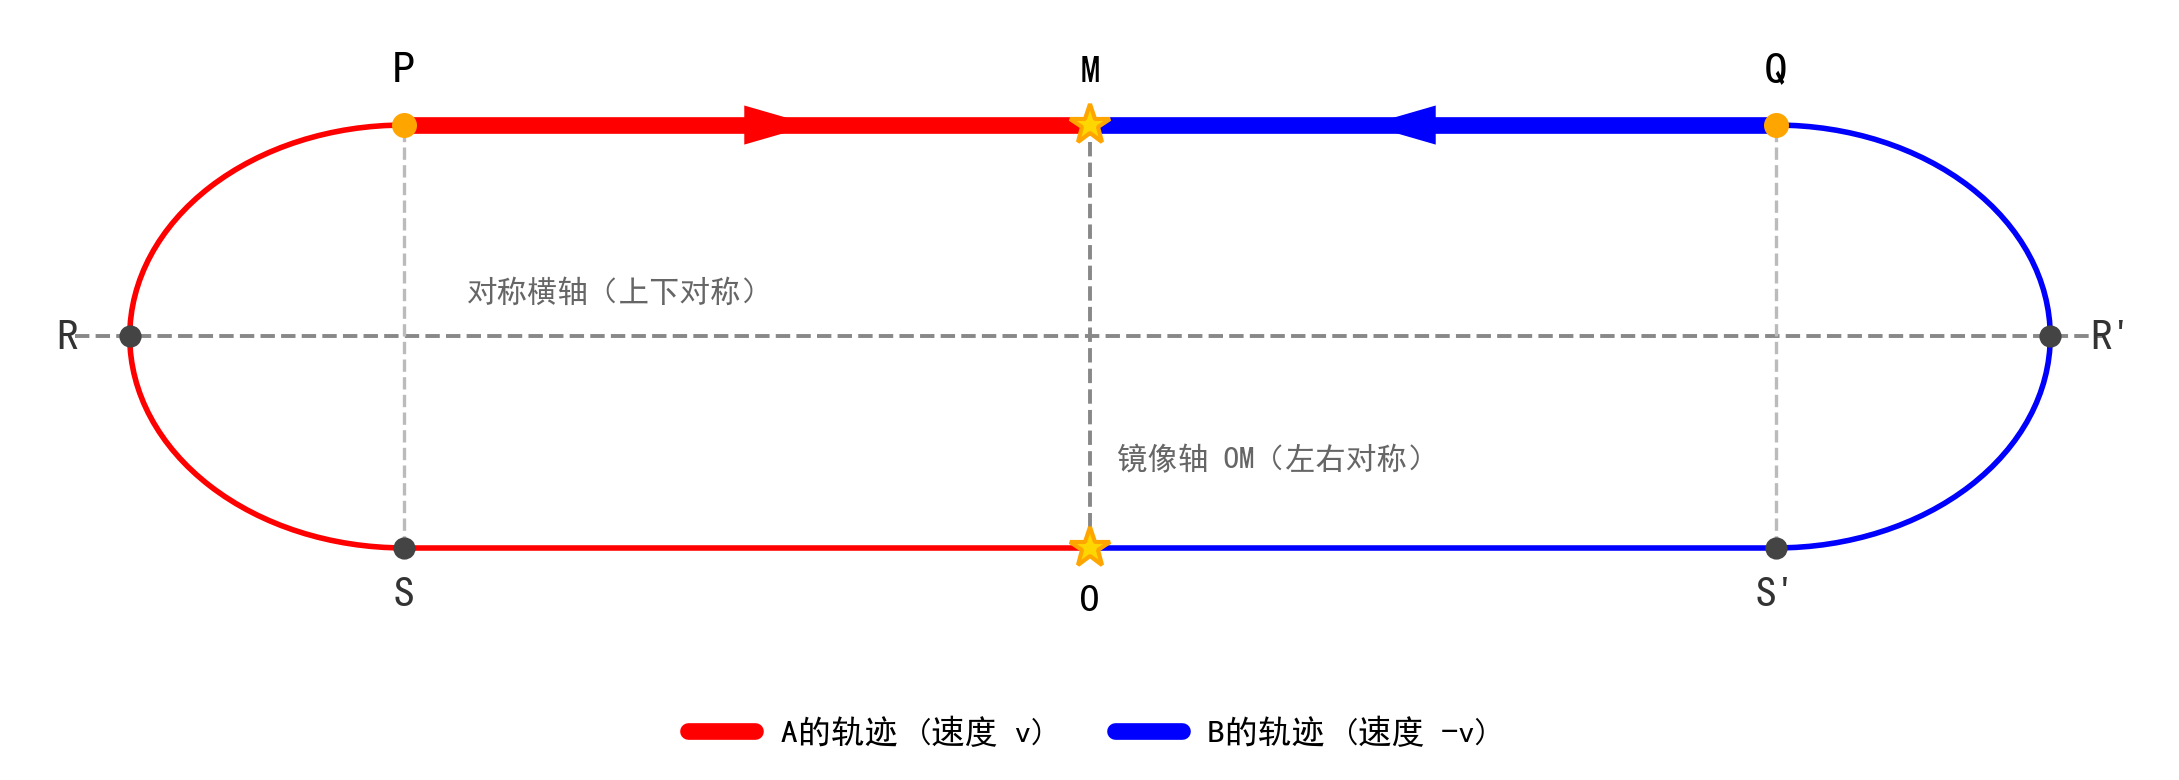
\includegraphics[width=0.92\linewidth,height=\textheight,keepaspectratio]{chapters/images/symmetric.png}

}

\caption{\label{fig-twins-comparison}对称双生子实验}

\end{figure}%

\begin{itemize}
\tightlist
\item
  在事件 \(O\) 处，A 与 B 相遇并对表，两者随身钟读数相同；
\item
  此后 A 经弧线到 \(P\)、B 经镜像弧线到 \(Q\)（这两段含加速与转向）；
\item
  自 \(P\) 起，A 沿直线以恒定速度向 \(M\) 运动；自 \(Q\) 起，B
  沿镜像直线以同样速率向 \(M\) 运动；
\item
  二者在 \(M\) 再次相遇。
\end{itemize}

\textbf{本章只研究直线段 \(P\to M\) 与
\(Q\to M\)}，即两段惯性运动。这是为了只使用匀速运动的变换公式，不引入加速情形的额外假设。

\subsection{坐标系}\label{ux5750ux6807ux7cfb}

取使两条直线段镜像对称的坐标系（\(x\) 轴水平，\(x=0\)
为对称轴），并把直线段的起点时刻记为 \(t=0\)。设
\(P=(-d,\,0)\)、\(Q=(+d,\,0)\)、\(M=(0,\,d/v)\)，其中 \(v\)
为直线段上的速率。

于是直线段上的两条轨迹为

\begin{equation}\protect\phantomsection\label{eq-trajectories}{
\text{A：}\ x_A(t)=-d+vt,\qquad \text{B：}\ x_B(t)=+d-vt
}\end{equation}

镜像映射 \(\iota(t,x):=(t,-x)\) 把 A 的轨迹映为 B 的轨迹：

\begin{equation}\protect\phantomsection\label{eq-iota-lines}{
\iota\bigl(t,\,-d+vt\bigr)=\bigl(t,\,d-vt\bigr)
}\end{equation}

\textbf{式~\ref{eq-iota-lines} 中两事件的时间分量相同，都是
\(t\)。这就是``对称对同时''。} 这句话的全部内容是：\(\iota\)
保持时间分量不变。它不需要任何外部参考系，也不需要任何观察者------时间方向是镜像对称自己挑出来的（\(\iota\)
的 \(+1\) 特征方向）。

\section{输入清单}\label{sec-tc-inputs}

三组输入彼此独立，本章分别使用，不混合。

\subsection{对称组（编号 S）}\label{ux5bf9ux79f0ux7ec4ux7f16ux53f7-s}

\textbf{(S1) 直线段完全镜像对称。} 由 式~\ref{eq-iota-lines} 表达。

\textbf{(S2) 起点读数相同。} 在 \(O\) 处两只钟读数相同。

\textbf{(S3) 钟的读数由该钟自身经历的过程决定。}
两只钟若经历完全相同的运动过程，其读数相同。

\subsection{洛伦兹组（编号
L）}\label{ux6d1bux4f26ux5179ux7ec4ux7f16ux53f7-l}

\textbf{(L1) 洛伦兹变换。} 相对速度 \(u\)
的两系之间（\(\gamma_u:=1/\sqrt{1-u^{2}/c^{2}}\)）：

\begin{equation}\protect\phantomsection\label{eq-L1}{
t'=\gamma_u\Bigl(t-\frac{u\,x}{c^{2}}\Bigr),\qquad x'=\gamma_u\,(x-ut)
}\end{equation}

\textbf{(L2)} 静止于某惯性系的钟，其读数等于该系的坐标时。

\subsection{伽利略组（编号
G）}\label{ux4f3dux5229ux7565ux7ec4ux7f16ux53f7-g}

\textbf{(G1) 伽利略变换。} 相对速度 \(u\) 的两系之间：

\begin{equation}\protect\phantomsection\label{eq-G1}{
t'=t,\qquad x'=x-ut
}\end{equation}

\textbf{(G2)} 与 (L2) 相同：静止于某惯性系的钟，其读数等于该系的坐标时。

\textbf{注意 (G1) 与 (L1) 的差别只在第一式}：一个说 \(t'=t\)，一个说
\(t'=\gamma_u(t-ux/c^{2})\)。本章的全部差别都从这一条产生。

\section{第一种算法：只用对称}\label{sec-tc-symmetry}

\begin{proposition}[对称对上两只钟读数相同]\protect\hypertarget{prp-tc-equal}{}\label{prp-tc-equal}

设 \(e_A\) 与 \(e_B\) 是直线段上的一对对称对（即
\(\iota(e_A)=e_B\)），则 \(\tau_A(e_A)=\tau_B(e_B)\)

\end{proposition}

\textbf{证明} 分三步。

\textbf{第一步}：由 (S1) 与 式~\ref{eq-iota-lines}，\(\iota\) 把 A 从
\(P\) 到 \(e_A\) 的整段过程映为 B 从 \(Q\) 到 \(e_B\)
的整段过程，两段过程的运动情形（速率大小、持续时间）逐一对应相同------反射只改变空间方向，不改变运动的任何其他内容。

\textbf{第二步}：由 (S3)，经历相同过程的两只钟，读数增量相同：

\begin{equation}\protect\phantomsection\label{eq-tc-inc}{
\tau_A(e_A)-\tau_A(P)=\tau_B(e_B)-\tau_B(Q)
}\end{equation}

\textbf{第三步}：由 (S2)，A 在 \(O\) 与 B 在 \(O\) 读数相同；而
\(O\to P\) 与 \(O\to Q\)
两段弧线亦互为镜像，同理（重复使用第二步与第三步）得
\(\tau_A(P)=\tau_B(Q)\)。把它代入
式~\ref{eq-tc-inc}，左端减左端、右端减右端：

\[
\begin{aligned}
\bigl[\tau_A(e_A)-\tau_A(P)\bigr]-\bigl[\tau_B(e_B)-\tau_B(Q)\bigr]&=0\\[4pt]
\tau_A(e_A)-\tau_B(e_B)-\bigl[\tau_A(P)-\tau_B(Q)\bigr]&=0\\[4pt]
\tau_A(e_A)-\tau_B(e_B)&=0
\end{aligned}
\]

即 \(\tau_A(e_A)=\tau_B(e_B)\)。

\subsection{跨系可知}\label{ux8de8ux7cfbux53efux77e5}

命题~\ref{prp-tc-equal} 的直接后果：\textbf{A
只要在本地读出自己的钟，就知道 B
的钟读的是什么数}------同一个数。这不是测量，不需要通信，不需要比对，也不需要第三者。

\subsection{比值}\label{ux6bd4ux503c}

由 命题~\ref{prp-tc-equal}，在对称对上 \(\tau_A=\tau_B\)
逐点成立，故沿直线段取微分：

\begin{equation}\protect\phantomsection\label{eq-tc-ratio-S}{
\boxed{\dfrac{\mathrm{d}\tau_B}{\mathrm{d}\tau_A}=1}
}\end{equation}

\section{第二种算法：只用洛伦兹变换}\label{sec-tc-lorentz}

本节不使用 (S1)---(S3)，只用 (L1)、(L2)。

\subsection{第一步：A 与 B
的相对速度}\label{ux7b2cux4e00ux6b65a-ux4e0e-b-ux7684ux76f8ux5bf9ux901fux5ea6}

由 式~\ref{eq-L1} 推出速度合成公式（标准推论，推导见
章节~\ref{sec-transform-derivation}）：两者相向运动、速率各为 \(v\)
时，相对速度大小为

\begin{equation}\protect\phantomsection\label{eq-tc-w}{
w=\frac{2v}{1+\dfrac{v^{2}}{c^{2}}},\qquad
\gamma_w=\frac{1}{\sqrt{1-\dfrac{w^{2}}{c^{2}}}}
=\frac{1+\dfrac{v^{2}}{c^{2}}}{1-\dfrac{v^{2}}{c^{2}}}
}\end{equation}

\subsection{第二步：B
的钟的两个相邻事件}\label{ux7b2cux4e8cux6b65b-ux7684ux949fux7684ux4e24ux4e2aux76f8ux90bbux4e8bux4ef6}

取 B 的钟上的两个相邻事件。在 B 的静止系中，B 的位置不变，故

\begin{equation}\protect\phantomsection\label{eq-tc-dxB}{
\mathrm{d}x_B=0,\qquad \mathrm{d}t_B=\mathrm{d}\tau_B\quad\text{（由 L2）}
}\end{equation}

\subsection{第三步：换到 A
系}\label{ux7b2cux4e09ux6b65ux6362ux5230-a-ux7cfb}

把这两个事件从 B 系换到 A 系。A 看 B 以速率 \(w\) 运动，由
式~\ref{eq-L1} 的第一式（取 \(u\) 为 A 系相对 B
系的速度，\(\gamma=\gamma_w\)）：

\begin{equation}\protect\phantomsection\label{eq-tc-dtA}{
\mathrm{d}t_A=\gamma_w\Bigl(\mathrm{d}t_B+\frac{w\,\mathrm{d}x_B}{c^{2}}\Bigr)
}\end{equation}

代入 式~\ref{eq-tc-dxB} 的第二式与第一式：

\begin{equation}\protect\phantomsection\label{eq-tc-dtA2}{
\mathrm{d}t_A=\gamma_w\Bigl(\mathrm{d}\tau_B+\frac{w\cdot 0}{c^{2}}\Bigr)=\gamma_w\,\mathrm{d}\tau_B
}\end{equation}

即

\begin{equation}\protect\phantomsection\label{eq-tc-tauB-L}{
\mathrm{d}\tau_B=\frac{\mathrm{d}t_A}{\gamma_w}
}\end{equation}

\subsection{第四步：A
自己的钟}\label{ux7b2cux56dbux6b65a-ux81eaux5df1ux7684ux949f}

A 在 A 系中静止，由 (L2)，A 的钟读数等于 A 系坐标时：

\begin{equation}\protect\phantomsection\label{eq-tc-tauA-L}{
\mathrm{d}\tau_A=\mathrm{d}t_A
}\end{equation}

\subsection{第五步：比值}\label{ux7b2cux4e94ux6b65ux6bd4ux503c}

把 式~\ref{eq-tc-tauA-L} 代入 式~\ref{eq-tc-tauB-L}：

\begin{equation}\protect\phantomsection\label{eq-tc-ratio-L}{
\boxed{\dfrac{\mathrm{d}\tau_B}{\mathrm{d}\tau_A}=\dfrac{1}{\gamma_w}}
}\end{equation}

由 式~\ref{eq-tc-w}，\(v\neq0\) 时 \(\gamma_w>1\)，故此比值小于
1。这就是``A 测得 B 的钟变慢''在洛伦兹框架中的数学内容。

\section{第三种算法：只用伽利略变换}\label{sec-tc-galilei}

本节不使用 (S1)---(S3)，也不使用 (L1)，只用 (G1)、(G2)。

\subsection{第一步：时间坐标是全局的}\label{ux7b2cux4e00ux6b65ux65f6ux95f4ux5750ux6807ux662fux5168ux5c40ux7684}

由 式~\ref{eq-G1}
的第一式，\(t'=t\)。\textbf{任意两个惯性系的时间坐标相同}，故所有系共享同一个时间坐标
\(t\)。

\subsection{第二步：两只钟的读数}\label{ux7b2cux4e8cux6b65ux4e24ux53eaux949fux7684ux8bfbux6570}

由 (G2)，静止于某惯性系的钟，其读数等于该系的坐标时。

\begin{itemize}
\tightlist
\item
  A 的钟静止于 A 系，故 \(\mathrm{d}\tau_A=\mathrm{d}t_A\)；而由
  式~\ref{eq-G1}，\(\mathrm{d}t_A=\mathrm{d}t\)。
\item
  B 的钟静止于 B 系，故 \(\mathrm{d}\tau_B=\mathrm{d}t_B\)；而由
  式~\ref{eq-G1}，\(\mathrm{d}t_B=\mathrm{d}t\)。
\end{itemize}

于是

\begin{equation}\protect\phantomsection\label{eq-tc-tau-G}{
\mathrm{d}\tau_A=\mathrm{d}t=\mathrm{d}\tau_B
}\end{equation}

\subsection{第三步：比值}\label{ux7b2cux4e09ux6b65ux6bd4ux503c}

\begin{equation}\protect\phantomsection\label{eq-tc-ratio-G}{
\boxed{\dfrac{\mathrm{d}\tau_B}{\mathrm{d}\tau_A}=1}
}\end{equation}

\section{三个答案并排}\label{sec-tc-table}

同一个问题：\textbf{A 的钟走一小段 \(\mathrm{d}\tau_A\) 时，B
的钟走多少？}

\begin{longtable}[]{@{}llll@{}}
\caption{三个答案}\label{tbl-tc-ratios}\tabularnewline
\toprule\noalign{}
& 输入 & 配对规则 & \(\mathrm{d}\tau_B/\mathrm{d}\tau_A\) \\
\midrule\noalign{}
\endfirsthead
\toprule\noalign{}
& 输入 & 配对规则 & \(\mathrm{d}\tau_B/\mathrm{d}\tau_A\) \\
\midrule\noalign{}
\endhead
\bottomrule\noalign{}
\endlastfoot
对称 & S1、S2、S3 & 对称对 \(\iota(e_A)=e_B\) & \(1\) \\
伽利略变换 & G1、G2 & 同一全局时间 \(t\) & \(1\) \\
洛伦兹变换 & L1、L2 & A 系同一坐标时 \(t_A\) & \(1/\gamma_w\) \\
\end{longtable}

\textbf{对称与伽利略给出同一个数（\(1\)），洛伦兹给出另一个数（\(1/\gamma_w\)）。}

\subsection{数值对照}\label{ux6570ux503cux5bf9ux7167}

取 \(v=0.6c\)。由 式~\ref{eq-tc-w}：

\[
w=\frac{2\times0.6c}{1+0.36}=0.8824c,\qquad
\gamma_w=\frac{1+0.36}{1-0.36}=2.125
\]

\begin{longtable}[]{@{}lll@{}}
\caption{\(v=0.6c\) 时的三个数}\label{tbl-tc-numeric}\tabularnewline
\toprule\noalign{}
& \(\mathrm{d}\tau_B/\mathrm{d}\tau_A\) & A 走 \(1\) 秒时 B 走 \\
\midrule\noalign{}
\endfirsthead
\toprule\noalign{}
& \(\mathrm{d}\tau_B/\mathrm{d}\tau_A\) & A 走 \(1\) 秒时 B 走 \\
\midrule\noalign{}
\endhead
\bottomrule\noalign{}
\endlastfoot
对称 & \(1\) & \(1\) 秒 \\
伽利略变换 & \(1\) & \(1\) 秒 \\
洛伦兹变换 & \(1/2.125=0.4706\) & \(0.4706\) 秒 \\
\end{longtable}

\subsection{对称对在 A
系中的坐标时差}\label{ux5bf9ux79f0ux5bf9ux5728-a-ux7cfbux4e2dux7684ux5750ux6807ux65f6ux5dee}

三个答案的差别还可以从另一处直接看出：\textbf{同一对对称对，在 A
系中的时间坐标是否相同？}

由 式~\ref{eq-trajectories}，对称对为 \(e_A=(t,\,-d+vt)\) 与
\(e_B=(t,\,+d-vt)\)。

\textbf{伽利略变换下}（\(t_A=t\)）：

\begin{equation}\protect\phantomsection\label{eq-tc-diff-G}{
t_A(e_B)-t_A(e_A)=t-t=0
}\end{equation}

\textbf{洛伦兹变换下}（\(t_A=\gamma_v(t-vx/c^{2})\)，A 沿 \(+x\)
运动，故 \(u=+v\)）：

\[
\begin{aligned}
t_A(e_A)&=\gamma_v\Bigl(t-\frac{v(-d+vt)}{c^{2}}\Bigr)=\gamma_v\Bigl(t+\frac{vd}{c^{2}}-\frac{v^{2}t}{c^{2}}\Bigr)\\[4pt]
t_A(e_B)&=\gamma_v\Bigl(t-\frac{v(+d-vt)}{c^{2}}\Bigr)=\gamma_v\Bigl(t-\frac{vd}{c^{2}}+\frac{v^{2}t}{c^{2}}\Bigr)
\end{aligned}
\]

两式相减，逐项相减：

\begin{equation}\protect\phantomsection\label{eq-tc-diff-L}{
\begin{aligned}
t_A(e_B)-t_A(e_A)
&=\gamma_v\Bigl(t-\frac{vd}{c^{2}}+\frac{v^{2}t}{c^{2}}\Bigr)-\gamma_v\Bigl(t+\frac{vd}{c^{2}}-\frac{v^{2}t}{c^{2}}\Bigr)\\[4pt]
&=\gamma_v\Bigl[\Bigl(t-t\Bigr)+\Bigl(-\frac{vd}{c^{2}}-\frac{vd}{c^{2}}\Bigr)+\Bigl(\frac{v^{2}t}{c^{2}}+\frac{v^{2}t}{c^{2}}\Bigr)\Bigr]\\[4pt]
&=\gamma_v\Bigl(-\frac{2vd}{c^{2}}+\frac{2v^{2}t}{c^{2}}\Bigr)\\[4pt]
&=\frac{2\gamma_v v}{c^{2}}\,(vt-d)
\end{aligned}
}\end{equation}

\textbf{检验}：在 \(t=d/v\)（即 \(M\) 处，由 式~\ref{eq-trajectories}
两者位置都是 \(x=0\)），式~\ref{eq-tc-diff-L} 给出 \(0\)------两事件在
\(M\) 处重合，坐标时必然相同，与计算一致。

\textbf{结论}：

\begin{longtable}[]{@{}
  >{\raggedright\arraybackslash}p{(\linewidth - 2\tabcolsep) * \real{0.5000}}
  >{\raggedright\arraybackslash}p{(\linewidth - 2\tabcolsep) * \real{0.5000}}@{}}
\caption{同时性是否随参考系改变}\label{tbl-tc-simultaneity}\tabularnewline
\toprule\noalign{}
\begin{minipage}[b]{\linewidth}\raggedright
变换
\end{minipage} & \begin{minipage}[b]{\linewidth}\raggedright
对称对在 A 系中的坐标时差
\end{minipage} \\
\midrule\noalign{}
\endfirsthead
\toprule\noalign{}
\begin{minipage}[b]{\linewidth}\raggedright
变换
\end{minipage} & \begin{minipage}[b]{\linewidth}\raggedright
对称对在 A 系中的坐标时差
\end{minipage} \\
\midrule\noalign{}
\endhead
\bottomrule\noalign{}
\endlastfoot
伽利略 & \(0\)（同时性不随参考系改变） \\
洛伦兹 & \(\dfrac{2\gamma_v v}{c^{2}}(vt-d)\)，一般非零（\(t\neq d/v\)
时） \\
\end{longtable}

\section{闵氏几何图：三种视角}\label{sec-tc-geometry}

前面的三个数来自代数。本节把同一件事画在闵氏几何图上。本节与前面的关系是：\textbf{(S)
组、(L) 组、(G)
组各自的配对规则，在图上各自对应一种几何形象}------对称配对的形象是校准双曲线，洛伦兹配对的形象是本系的同时线，伽利略配对的形象是与参考系无关的水平直线。三个视角（A、B、地球）各画一张图，最后看伽利略极限下图形如何变化。

\subsection{从前文的坐标系到 A
视角}\label{ux4eceux524dux6587ux7684ux5750ux6807ux7cfbux5230-a-ux89c6ux89d2}

式~\ref{eq-trajectories} 写在 小节~\ref{sec-tc-setup}
的镜像对称系中（本节右图``地球视角''沿用这一系）。画 A 视角图只需两步：

\begin{enumerate}
\def\labelenumi{\arabic{enumi}.}
\tightlist
\item
  \textbf{平移}：把 A 的直线段起点 \(P\) 平移到原点
  \(O\)。平移不改变任何一只钟的任何一段读数（所有钟的读数增量照旧），只改变事件的名字。
\item
  \textbf{换系}：用 (L1) 把坐标换到 A 的静止系。A 在 A 系中静止，故 A
  的世界线是纵轴本身；B 在 A 系中做惯性运动，速率由 式~\ref{eq-tc-w}
  给出（两系相向、各以 \(v\) 运动，相对速率 \(w\)），世界线是过 \(O\)
  的直线
\end{enumerate}

\[
x=-wt.
\]

以下三张图里，横轴都是 A 系（或相应系）的空间坐标
\(x\)，纵轴都是时间坐标 \(t\)，\(\tau\) 是任取的一个读数单位；数值沿用
表~\ref{tbl-tc-numeric} 的 \(v=0.6c\)，即
\(w=0.8824c\)、\(\gamma_w=2.125\)。

\subsection{第一步：把钟的读数标注到图上}\label{ux7b2cux4e00ux6b65ux628aux949fux7684ux8bfbux6570ux6807ux6ce8ux5230ux56feux4e0a}

由 (L2)：静止于某惯性系的钟，读数等于该系的坐标时。

\begin{itemize}
\tightlist
\item
  \textbf{A 的钟}：A 静止于 A 系，故 A 的读数就是纵轴上的 \(t\)
  本身------A 世界线上每个事件直接按 \(t\) 标读数。
\item
  \textbf{B 的钟}：B 静止于 B 系，B 的读数等于 B 系坐标时 \(t_B\)。B
  世界线上、A 系坐标时为 \(t\) 的事件，其 B 读数由 (L1) 算出：B 系相对 A
  系以 \(-w\) 运动，故 \(t_B=\gamma_w\bigl(t+w\,x/c^{2}\bigr)\)；代入 B
  的世界线 \(x=-wt\)：
\end{itemize}

\begin{equation}\protect\phantomsection\label{eq-tc-Bclock}{
t_B=\gamma_w\bigl(t-w^{2}t/c^{2}\bigr)=\gamma_w\,t\bigl(1-w^{2}/c^{2}\bigr)=\frac{t}{\gamma_w}.
}\end{equation}

即：\textbf{B 世界线上坐标时为 \(t\) 的事件，B 的钟读数是
\(t/\gamma_w\)}。在图上，B 的读数刻度沿 B
的世界线越往上越``疏''------同一个读数 \(\tau\)，在 A 的纵轴上位于
\(t=\tau\)，在 B 的世界线上位于 \(t=\gamma_w\tau\)。

\subsection{第二步：等读数点的轨迹}\label{ux7b2cux4e8cux6b65ux7b49ux8bfbux6570ux70b9ux7684ux8f68ux8ff9}

现在问一个只涉及几何的问题：从 \(O\) 出发、以任意恒定速度 \(u\)
运动的钟，当它读数为 \(\tau\) 时，它所在的事件在图上构成什么曲线？

由 (L2) 与 (L1)（与 式~\ref{eq-tc-Bclock} 同样的计算）：这个钟的读数是
\(t\sqrt{1-u^{2}/K^{2}}\)，其中 \(K\) 是不变量速度（第
章节~\ref{sec-invariant-speed-group} 章；\(K=c\) 为洛伦兹，\(K=\infty\)
为伽利略）。令读数等于 \(\tau\)，得
\(t=\tau\big/\sqrt{1-u^{2}/K^{2}}\)。事件坐标是 \((t,\,x=ut)\)，故
\(u=x/t\)，代入：

\begin{proposition}[等固有读数点的轨迹是校准双曲线]\protect\hypertarget{prp-tc-hyperbola}{}\label{prp-tc-hyperbola}

从 \(O\) 出发、以任意恒定速度运动的钟读数为 \(\tau\) 的全部事件构成曲线

\begin{equation}\protect\phantomsection\label{eq-tc-hyperbola}{
t^{2}-\frac{x^{2}}{K^{2}}=\tau^{2},
}\end{equation}

且该曲线与 B 的世界线 \(x=-wt\) 交于 B 读数恰为 \(\tau\) 的一点，其 A
系坐标时为 \(\gamma_w\tau\)。

\end{proposition}

\textbf{证明}：上面两行代入已是证明。与 B 世界线的交点：取 \(u=-w\)，则
\(t=\tau\big/\sqrt{1-w^{2}/K^{2}}=\gamma_w\tau\)，由
式~\ref{eq-tc-Bclock} 该点的 B 读数为 \(\gamma_w\tau/\gamma_w=\tau\)。

曲线的形状值得看清：\(x=0\) 处 \(t=\tau\)（最低点）；\(|x|\) 越大 \(t\)
越大；渐近线是光锥 \(x=\pm Kt\)。它是\textbf{凹向 \(t\)
轴的双曲线}，不是圆。

\textbf{与圆弧的对照。} 一种常见的直觉是``以 \(O\) 为圆心、\(OM_t\)
为半径画圆弧，用它在两条世界线之间定位对称点''。这个做法不成立：在 A
视角的标准闵氏图中，\textbf{欧氏圆 \(t^{2}+x^{2}=\tau^{2}\)
不是任何钟的读数轨迹}------它到原点的距离是欧氏距离，而钟读数走的是
式~\ref{eq-tc-hyperbola}。欧氏圆与 式~\ref{eq-tc-hyperbola} 仅在
\(u=0\)（即 \(M_t\) 本身）相触；圆弧与 B 世界线的交点上，钟的读数是

\[
\tau\sqrt{\frac{1-w^{2}/K^{2}}{1+w^{2}/K^{2}}}\ \neq\ \tau,
\]

故圆弧交点\textbf{不是}对称点：它把对称点画近了。修正只改变图中对称点与投影点的\textbf{位置}，不改变本章的任何结论：对称配对上读数相同（命题~\ref{prp-tc-equal}）、洛伦兹配对给出
\(1/\gamma_w\)（式~\ref{eq-tc-ratio-L}）、两套配对是不同的配对（表~\ref{tbl-tc-ratios}），全部保持。

\subsection{第三步：两套配对的形象}\label{ux7b2cux4e09ux6b65ux4e24ux5957ux914dux5bf9ux7684ux5f62ux8c61}

``配对规则''的几何形象是一条把两个事件连成一对的\textbf{线}。

\begin{itemize}
\tightlist
\item
  \textbf{对称配对（S 组）}：命题~\ref{prp-tc-equal}
  配的是对称点对------A 读 \(\tau\) 的事件 \(M_t=(\tau,0)\) 与 B 读
  \(\tau\) 的事件 \(M_{t'}\)。由 命题~\ref{prp-tc-hyperbola}，这些点对沿
  式~\ref{eq-tc-hyperbola} 排列。\textbf{对称配对的形象是校准双曲线}。
\item
  \textbf{洛伦兹配对（L 组）}：式~\ref{eq-tc-ratio-L} 配的是``A
  系坐标时相等''的事件。A 系的同时线在 A 视角图中是水平线 \(t=\) 常数（A
  系的坐标时就是纵轴）。\textbf{洛伦兹配对的形象是水平线}。
\end{itemize}

\begin{corollary}[投影时与对称读数]\protect\hypertarget{cor-tc-projection}{}\label{cor-tc-projection}

过 B 读 \(\tau\) 的对称点 \(M_{t'}\) 作水平线（A 系同时线），交 A
的世界线于 A 系坐标时 \(\gamma_w\tau\) 处：\textbf{投影时
\(=\gamma_w\tau>\tau\)，投影点在 \(M_t\) 上方}。反过来，过 A 读 \(\tau\)
的事件 \(M_t\) 作水平线，交 B 世界线于 B 读 \(\tau/\gamma_w\)
处（式~\ref{eq-tc-Bclock}）。两个数之比 \(\gamma_w\)
全部来自``用哪条线配对''的选择，不来自任何一只钟的内部。

\end{corollary}

\subsection{三视角对照}\label{ux4e09ux89c6ux89d2ux5bf9ux7167}

\begin{figure}

\centering{

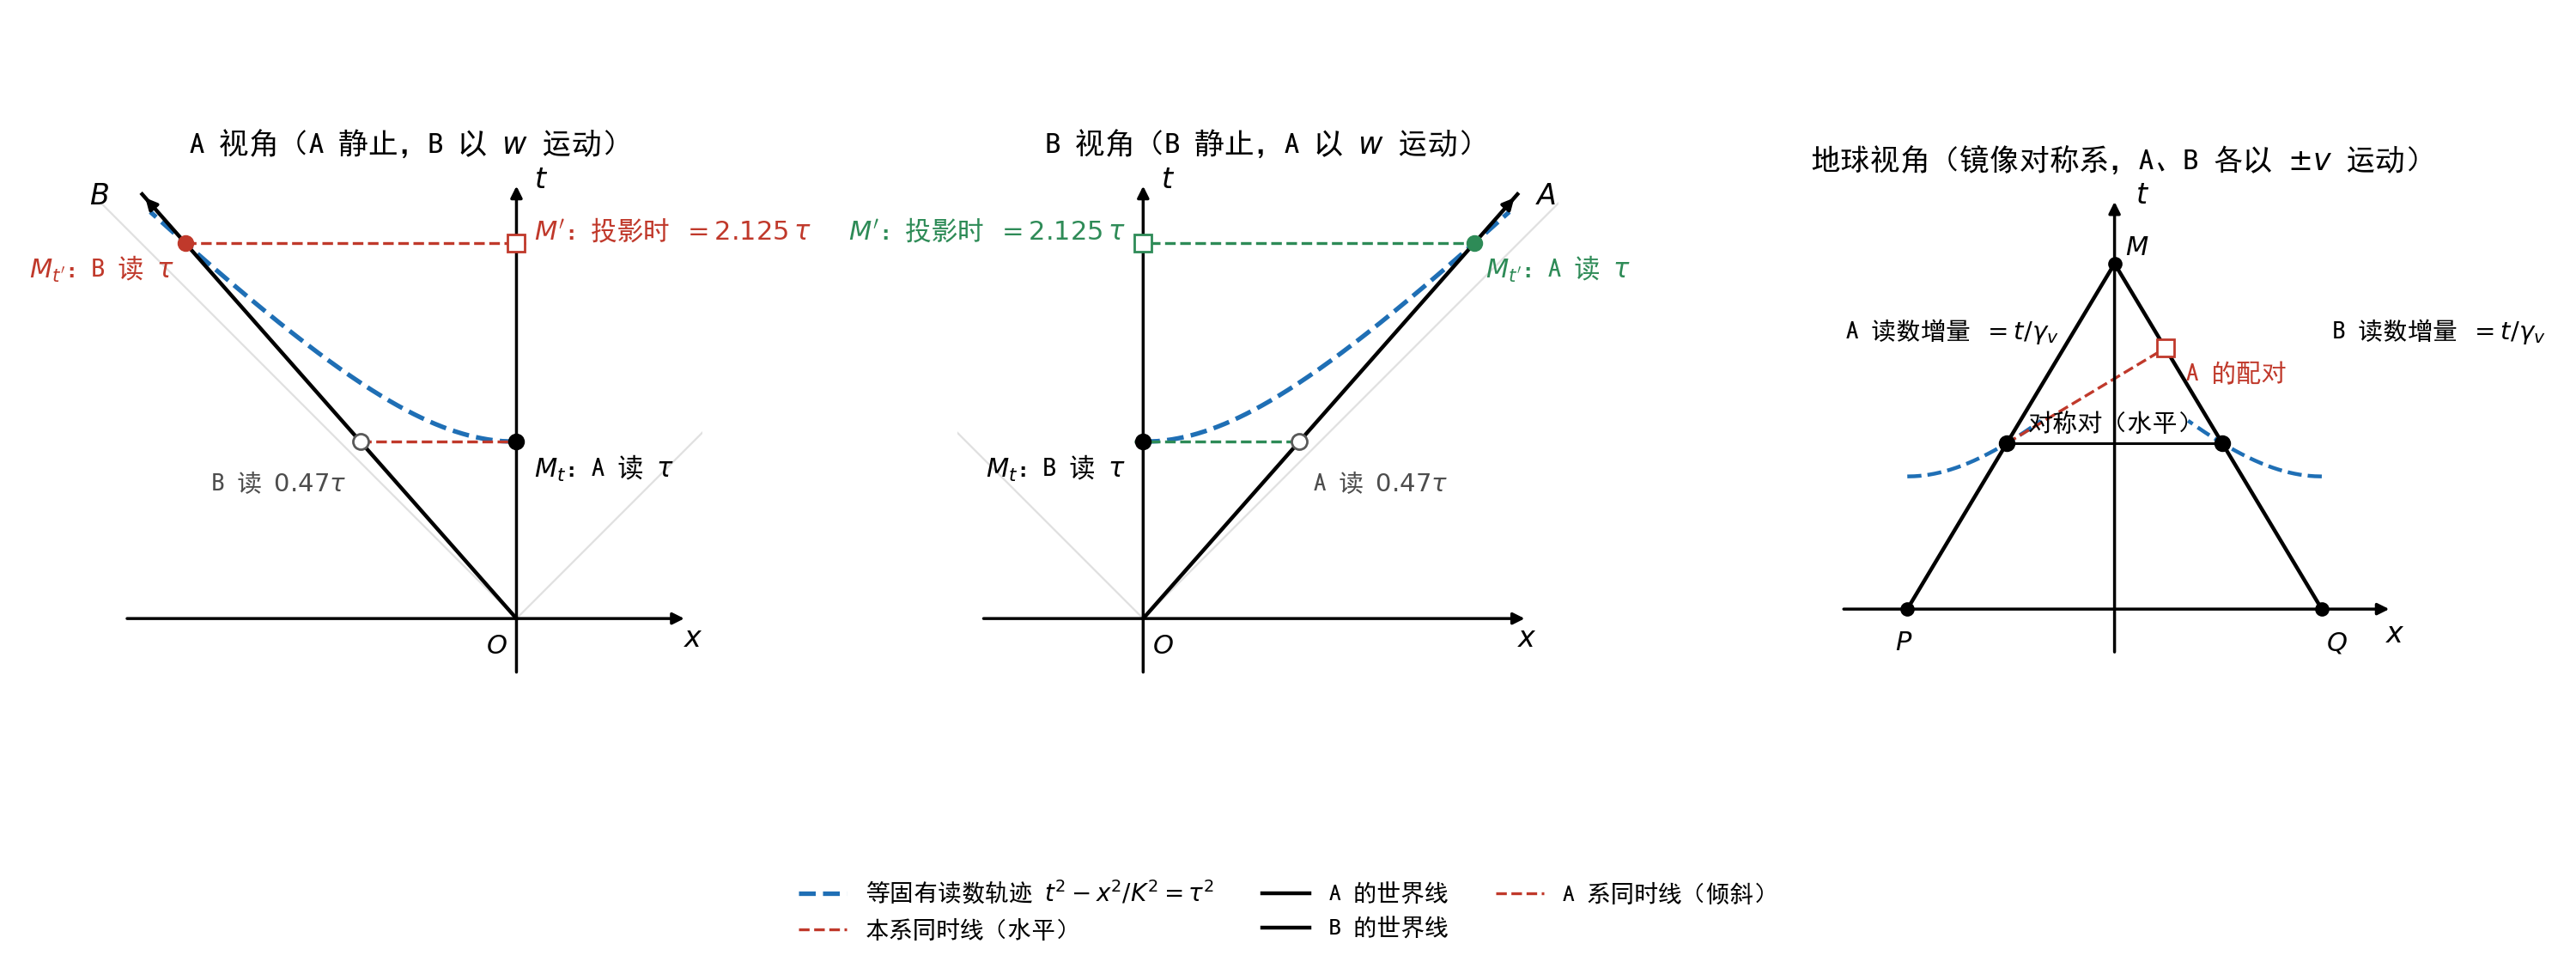
\includegraphics[width=1\linewidth,height=\textheight,keepaspectratio]{chapters/images/twins-three-views.png}

}

\caption{\label{fig-tc-three-views}对称双生子的三视角闵氏几何图（\(v=0.6c\)，\(w=0.8824c\)，\(\gamma_w=2.125\)）}

\end{figure}%

\textbf{左：A 视角。} 图上同时画着两套配对线。蓝色虚线是校准双曲线
式~\ref{eq-tc-hyperbola}：\(M_t\)（A 读 \(\tau\)）与 \(M_{t'}\)（B 读
\(\tau\)）在同一条双曲线上------这是 (S) 组的配对，读数相同，且 A
在本地读出 \(\tau\) 就知道 B 也是
\(\tau\)，无需测量（命题~\ref{prp-tc-equal}
的``跨系可知''）。红色虚线是水平线（A 系同时线）：过 \(M_t\) 的水平线交
B 世界线于 B 读 \(0.47\tau=\tau/\gamma_w\) 处，过 \(M_{t'}\) 的水平线交
A 世界线于投影点 \(M'\)（A 系坐标时
\(\gamma_w\tau=2.125\tau\)）------这是 (L) 组的配对，B 的读数落后一个
\(\gamma_w\) 因子，正是 式~\ref{eq-tc-ratio-L} 的几何形式。

\textbf{中：B 视角。} 把左图作镜像 \(x\to-x\)、A 与 B
互换，得到完全相同的图：B 静止，A 以 \(w\) 沿 \(+x\)
运动，双曲线、投影、比值逐一对应。这就是``B 看 A
只是身份互换，效果等价''的几何内容：两张图互为镜像，没有任何一张拥有特殊地位。

\textbf{右：地球视角。} 这就是 小节~\ref{sec-tc-setup}
的镜像对称系（式~\ref{eq-trajectories} 的主坐标系）：A、B 各以 \(\pm v\)
运动。三件事值得逐一指出：

\begin{enumerate}
\def\labelenumi{\arabic{enumi}.}
\tightlist
\item
  \textbf{对称配对与同时配对在此重合。} 由
  式~\ref{eq-iota-lines}，对称对 \(\iota(e_A)=e_B\)
  的时间分量相同------对称对落在同一条水平线上。故 (S)
  组的配对与``地球系坐标时相等''的配对（用 (L2)
  与地球系坐标）是同一套配对。双曲线弧（以 \(P\)、\(Q\) 为心的
  式~\ref{eq-tc-hyperbola}，因两钟直线段的读数从 \(P\)、\(Q\)
  起算）分别穿过两个对称点。
\item
  \textbf{同一水平线上三只钟的读数。} A 与 B 的读数增量都是
  \(t/\gamma_v\)（两者相同------(S) 组结论在图上的样子），地球钟是
  \(t\)。地球视角中的``钟慢''是 A、B 各自相对地球的，\textbf{不是 A 与 B
  相互的}。
\item
  \textbf{A 系同时线在此系中倾斜。} 由 (L1) 第一式
  \(t_A=\gamma_v\bigl(t-vx/c^{2}\bigr)\)，令 \(t_A\) 为常数得
  \(t=\text{常数}+(v/c^{2})x\)：斜率 \(v/c^{2}>0\) 的直线。它过 A
  世界线上 \((t,\,-d+vt)\) 的事件，与 B 世界线 \(x=d-vt\) 联立，交点为
\end{enumerate}

\begin{equation}\protect\phantomsection\label{eq-tc-tprime}{
t'=\frac{t\bigl(1-v^{2}/c^{2}\bigr)+2vd/c^{2}}{1+v^{2}/c^{2}}.
}\end{equation}

\(t\to\infty\) 时 B 与 A 的读数增量比趋于
\((1-v^{2}/c^{2})/(1+v^{2}/c^{2})=1/\gamma_w\)，与
式~\ref{eq-tc-ratio-L} 一致（符号核验：\(v=0.6c\) 时该比为
\((15d+8t)/(17t)\)，极限 \(8/17\)）。有限 \(t\) 处的偏差来自
\(P\neq Q\)------两钟的读数在弧线段上已有偏移；这正是
式~\ref{eq-tc-ratio-L} 采用微分形式的原因，也是 式~\ref{eq-tc-key}
中那个差一项的来源。

\subsection{物理诠释：两只寿命八十年的钟}\label{sec-tc-lifespan}

把 \(\tau\) 取成一个具体的数，配对差就变成看得见的东西。设 A 与 B
都是寿命八十年的生命（或寿命八十年的钟）------``寿命''指各自随身钟的读数从
\(O\) 走到 80。

\textbf{对称判据（(S) 组）：两人都活到了 80 岁。} A 活到 80 岁的事件
\(e_A\) 与 B 活到 80 岁的事件 \(e_B\)
互为对称点（\(\iota(e_A)=e_B\)，式~\ref{eq-iota-lines}），由
命题~\ref{prp-tc-equal} 两者读数相同。这是本章的``同时''：A
在本地读出自己的 80，就知道 B 也是
80------不需要测量，不需要通信，不需要第三者。

\textbf{洛伦兹测量（(L) 组）：A 测得 B 的读数落后。} A 在自己 80
岁的``现在''作 A 系同时线（左图的水平线），它与 B 的世界线交于 B 读
\(80/\gamma_w\) 岁的事件。按 表~\ref{tbl-tc-numeric} 的
\(\gamma_w=2.125\)，这个数是 \(37.6\) 岁；相对速度更小时更接近 80（例如
\(w\approx0.5c\) 时约 69 岁）------但只要 \(w\neq0\)，它总比 80
小。反过来，B 的 80 岁事件 \(M_{t'}\) 在 A 的水平线上配到 A 读
\(\gamma_w\times80=170\) 岁：A 要活到 170 岁，自己的``现在''才碰到 B 的
80 岁。

这就是``基于钟慢效应的时空旅行不成立''的物理内容：钟慢从不缩短任何一只钟自己的寿命------它只是
A 的``现在''切片在 B 的世界线上切得偏早。切片的偏移随 \(K\to\infty\)
消失（下一节），随 \(K\to c\) 增大；它在任何情况下都不是生命本身的改变。

\section{伽利略极限}\label{sec-tc-galilean-geometry}

式~\ref{eq-tc-hyperbola} 含有参数 \(K\)。令 \(K\)
变化，就得到从洛伦兹到伽利略的连续过渡：

\begin{figure}

\centering{

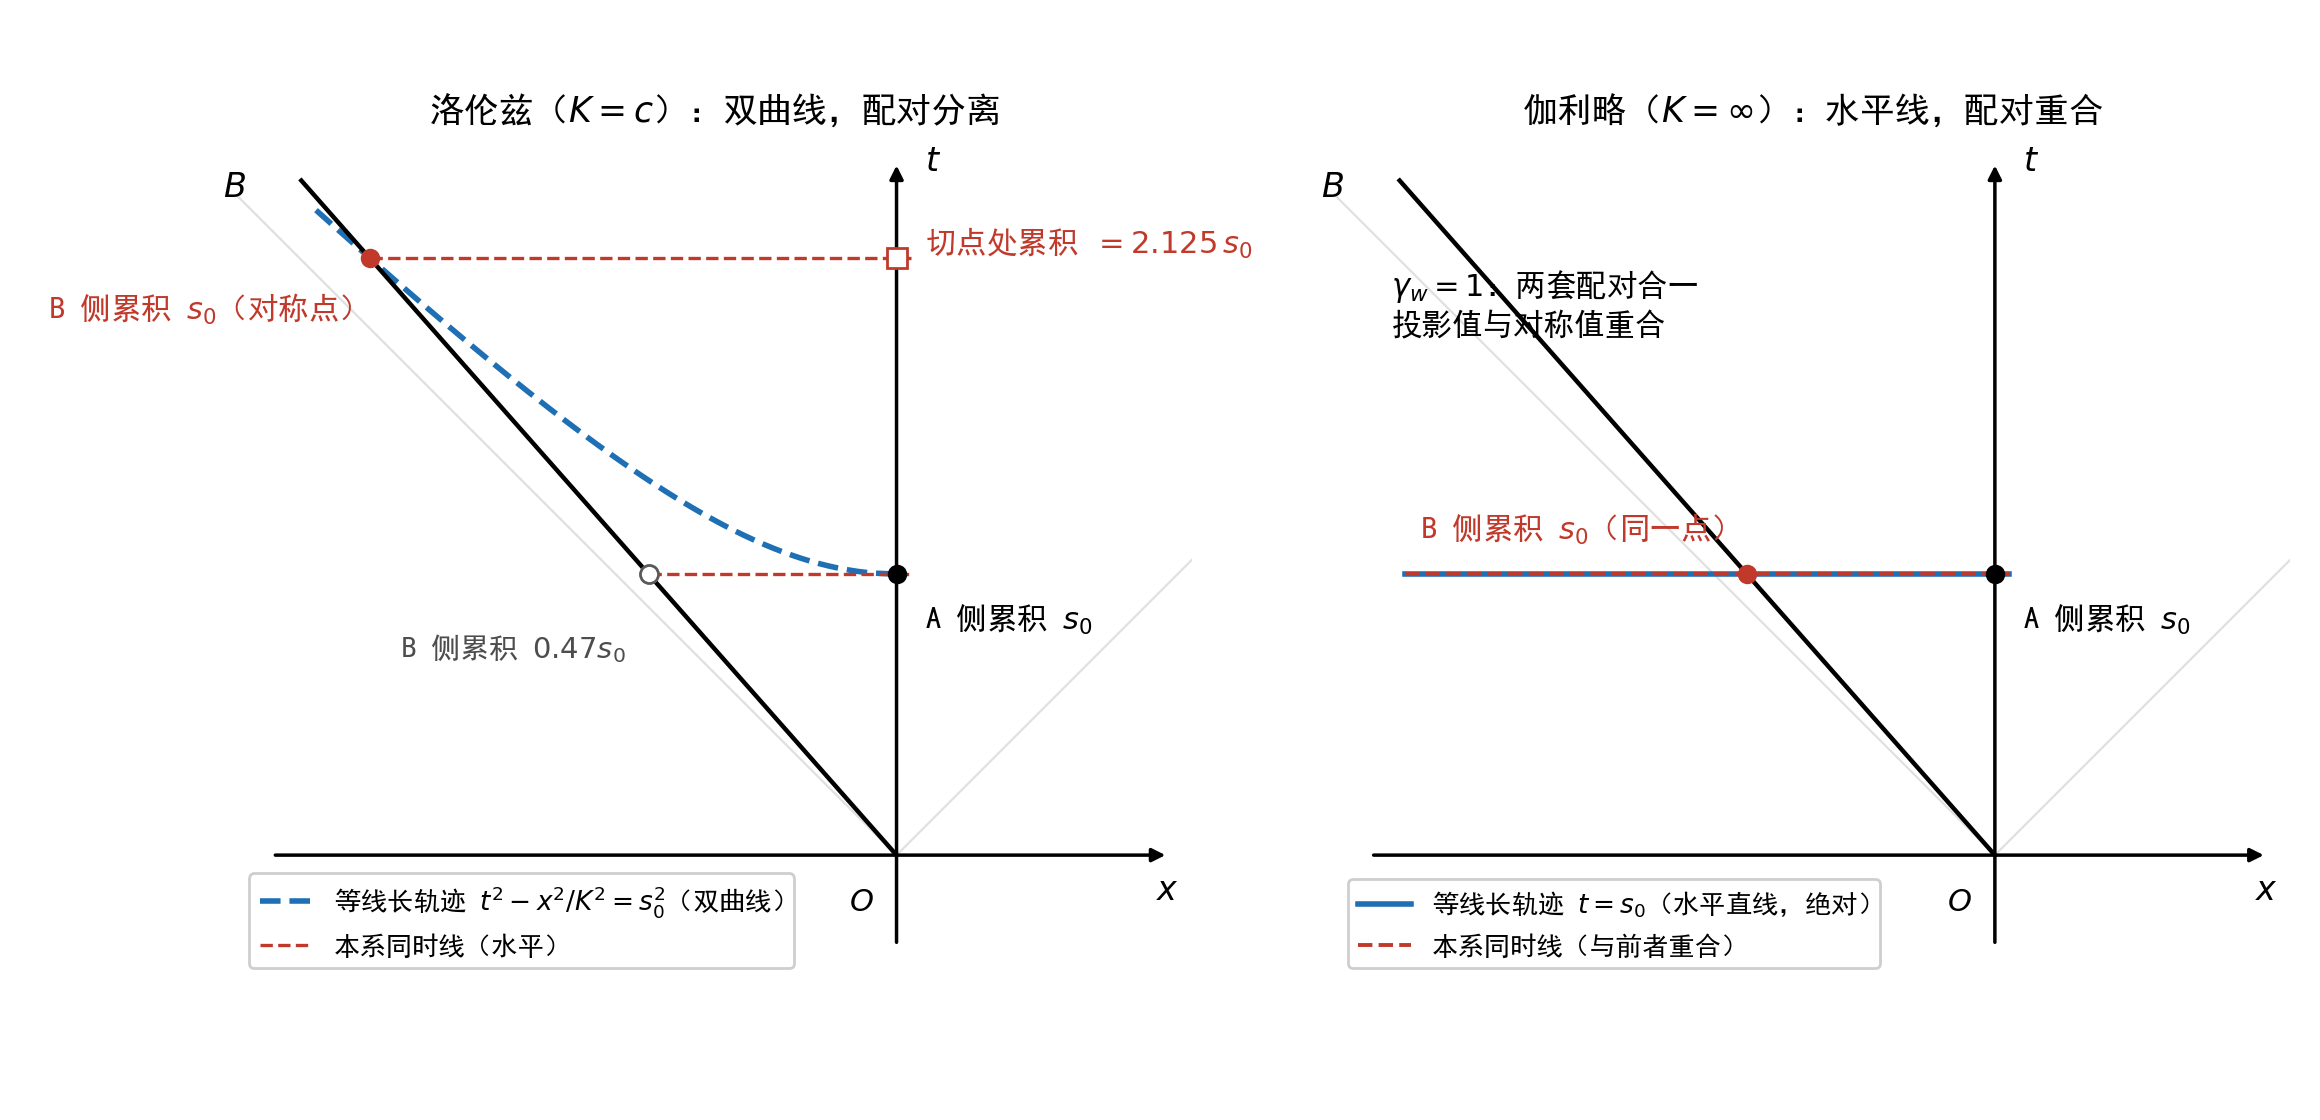
\includegraphics[width=1\linewidth,height=\textheight,keepaspectratio]{chapters/images/twins-galilean-compare.png}

}

\caption{\label{fig-tc-galilean}洛伦兹与伽利略的对照：等读数轨迹从双曲线变为水平直线}

\end{figure}%

\textbf{双曲线的退化。} \(K\to\infty\) 时 式~\ref{eq-tc-hyperbola} 中
\(x^{2}/K^{2}\to0\)，曲线变为水平直线
\(t=\tau\)------\textbf{与参考系无关的绝对同时面}。对称点的 A 系坐标时
\(\gamma_w\tau\to\tau\)：投影时与对称读数重合，推论~\ref{cor-tc-projection}
中的两个配对合一。这与 式~\ref{eq-tc-diff-G}（伽利略下对称对坐标时差为
\(0\)）是同一件事的两种说法。

\textbf{\(\gamma_w\) 随 \(K\) 的变化}（固定 \(w=0.8824c\)）：

\begin{longtable}[]{@{}lllll@{}}
\caption{投影分歧随不变量速度 \(K\)
的变化}\label{tbl-tc-gamma}\tabularnewline
\toprule\noalign{}
\(K\) & \(\infty\) & \(3c\) & \(1.5c\) & \(c\) \\
\midrule\noalign{}
\endfirsthead
\toprule\noalign{}
\(K\) & \(\infty\) & \(3c\) & \(1.5c\) & \(c\) \\
\midrule\noalign{}
\endhead
\bottomrule\noalign{}
\endlastfoot
\(\gamma_w\) & \(1\) & \(1.046\) & \(1.237\) & \(2.125\) \\
\end{longtable}

\textbf{结论}：投影分歧 \(\gamma_w-1\) 全部来自 式~\ref{eq-tc-hyperbola}
中的 \(1/K^{2}\) 项。\(K\)
有限时等读数轨迹是双曲线，各系的同时线互不平行，配对分离（图~\ref{fig-tc-galilean}
左）；\(K\to\infty\)
时曲线拉平为直线，所有系共享同一同时面，配对重合（图~\ref{fig-tc-galilean}
右）。用 小节~\ref{sec-tc-lifespan} 的比喻说：\(K\to\infty\)
时所有人的``书签''都水平，插的位置与书的页码一致------书签与书页不再有差。这与第
章节~\ref{sec-invariant-speed-group} 章的群收缩（结构常数
\(1/K^{2}\to0\)）和第 章节~\ref{sec-quantum-phase}
章量子相态的条件（\(K\to\infty\) 且 \(\vec\nabla K=0\)）是同一个极限。

\section{只用变换能推出什么}\label{sec-tc-only-transform}

作为对照：如果\textbf{完全不使用对称}，只使用变换与
(L2)/(G2)，能推出什么？

记 \(\Delta\tau_A\) 为 A 的钟在 \(P\to M\)
上的读数增量，\(\Delta\tau_B\) 为 B 的钟在 \(Q\to M\) 上的读数增量。

\textbf{洛伦兹情形}：只用 (L1)、(L2)，推导如下。由 (L2)：A 在 A
系中静止，故 \(\Delta\tau_A=t_A^{M}-t_A^{P}\)；B 在 B 系中静止，故
\(\Delta\tau_B=t_B^{M}-t_B^{Q}\)。对 B 的这两个事件用 (L1) 换到 A 系：B
在 B 系中位置不变（\(x_B\) 为常数），故

\[
t_A^{M}-t_A^{Q}=\gamma_w\Bigl[\bigl(t_B^{M}-t_B^{Q}\bigr)+\frac{w\,\bigl(x_B^{M}-x_B^{Q}\bigr)}{c^{2}}\Bigr]=\gamma_w\,\Delta\tau_B,
\]

再代入
\(\Delta\tau_A=t_A^{M}-t_A^{P}\)，逐项相减，得到的\textbf{全部}约束是

\begin{equation}\protect\phantomsection\label{eq-tc-key}{
t_A^{P}-t_A^{Q}=\gamma_w\,\Delta\tau_B-\Delta\tau_A
}\end{equation}

其中 \(t_A^{P}\)、\(t_A^{Q}\) 是 \(P\)、\(Q\) 两事件在 A
系中的时间坐标。要由此得到
\(\Delta\tau_A=\Delta\tau_B\)，需要右端为零，即
\(\Delta\tau_A=\gamma_w\Delta\tau_B\)------\textbf{这个等式不属于
(L1)，也不属于 (L2)}。

\textbf{伽利略情形}：由
式~\ref{eq-tc-tau-G}，\(\mathrm{d}\tau_A=\mathrm{d}t=\mathrm{d}\tau_B\)
直接成立，积分得

\begin{equation}\protect\phantomsection\label{eq-tc-equal-G}{
\Delta\tau_A=\Delta\tau_B
}\end{equation}

这是 (G1)、(G2) 的推论，\textbf{不需要借助对称}。

\textbf{结论}：

\begin{longtable}[]{@{}
  >{\raggedright\arraybackslash}p{(\linewidth - 2\tabcolsep) * \real{0.5000}}
  >{\raggedright\arraybackslash}p{(\linewidth - 2\tabcolsep) * \real{0.5000}}@{}}
\caption{只用变换能推出什么}\label{tbl-tc-only}\tabularnewline
\toprule\noalign{}
\begin{minipage}[b]{\linewidth}\raggedright
\end{minipage} & \begin{minipage}[b]{\linewidth}\raggedright
只用变换能否推出 \(\Delta\tau_A=\Delta\tau_B\)
\end{minipage} \\
\midrule\noalign{}
\endfirsthead
\toprule\noalign{}
\begin{minipage}[b]{\linewidth}\raggedright
\end{minipage} & \begin{minipage}[b]{\linewidth}\raggedright
只用变换能否推出 \(\Delta\tau_A=\Delta\tau_B\)
\end{minipage} \\
\midrule\noalign{}
\endhead
\bottomrule\noalign{}
\endlastfoot
洛伦兹变换 & \textbf{不能}（还差一个条件
\(\Delta\tau_A=\gamma_w\Delta\tau_B\)） \\
伽利略变换 & \textbf{能}（\(t'=t\) 的直接推论） \\
\end{longtable}

\section{地球版双生子}\label{sec-twins-absolute}

\subsection{本节做什么}\label{sec-ta-scope}

前面处理的是\textbf{对称}实验：两人镜像飞离、镜像折返，三套输入（对称、洛伦兹、伽利略）各给出一个数。本节换一个实验------\textbf{地球版双生子}：弟弟留在地球，哥哥一个人飞出去一圈再回来。这是一个\textbf{不对称}的实验，掉头的只有一个人。

本节把同一个实验放进恒速群的两端：\(K=c\) 与
\(K=\infty\)。两支各列其公理，各推其结果，并列摆放。

\subsection{实验设定}\label{sec-ta-setup}

\begin{definition}[地球版双生子]\protect\hypertarget{def-ta-setup}{}\label{def-ta-setup}

在地球系中，弟弟 \(D\) 始终停留在 \(x=0\)；哥哥 \(G\) 以速率 \(v\)
沿直线飞离到 \(x=d\)，掉头后以同样速率飞回，在事件 \(R\) 与 \(D\)
重逢。记 \(O\) 为分离事件，取地球系全程时间 \(T=2d/v\)。

\end{definition}

与第 章节~\ref{sec-symmetric-twins}
章的镜像实验相比，差别只有一条：\textbf{掉头的只有一个人}。\(D\)
的世界线是一条直线，\(G\) 的世界线是一条折线，两者不互为镜像。

\subsection{\texorpdfstring{第一支：\(K=c\)}{第一支：K=c}}\label{sec-ta-branch-c}

\begin{conjecture}[洛伦兹公设（\(K=c\)）]\protect\hypertarget{cnj-ta-lorentz}{}\label{cnj-ta-lorentz}

恒速群取 \(K=c\)，即存在有限的不变速度 \(c\)。据此：

\begin{enumerate}
\def\labelenumi{\arabic{enumi}.}
\tightlist
\item
  \textbf{变换}：\(t'=\gamma_u\bigl(t-ux/c^{2}\bigr)\)，\(x'=\gamma_u(x-ut)\)，其中
  \(\gamma_u=1/\sqrt{1-u^{2}/c^{2}}\)。
\item
  \textbf{同时}：同时性随参考系改变，同时面为
  \(t-ux/c^{2}=\text{常数}\)。
\item
  \textbf{读数尺度}：\(\mathrm{d}s^{2}=\mathrm{d}t^{2}-\mathrm{d}x^{2}/c^{2}\)。
\end{enumerate}

\end{conjecture}

\begin{proposition}[在该公设下：读数沿各自的路径累积]\protect\hypertarget{prp-ta-lorentz-result}{}\label{prp-ta-lorentz-result}

\[
\Delta\tau=\int_{\gamma}\mathrm{d}s=\int_{\gamma}\sqrt{\mathrm{d}t^{2}-\mathrm{d}x^{2}/c^{2}}
\]

对 \(D\)（\(x=0\)）：\(\Delta\tau_D=T\)。对 \(G\)（两段匀速、速率
\(v\)、忽略掉头段）：

\[
\Delta\tau_G=T\sqrt{1-v^{2}/c^{2}}=\frac{T}{\gamma},\qquad \gamma=\frac{1}{\sqrt{1-v^{2}/c^{2}}}
\]

\end{proposition}

由此得到：\(v\neq0\) 时 \(\Delta\tau_G<\Delta\tau_D\)，重逢时 \(G\)
的读数小于 \(D\) 的读数。掉头段只通过它占用的 \(\mathrm{d}t\)
进入积分；令掉头段历时趋于零，上式不变。

\subsection{\texorpdfstring{第二支：\(K=\infty\)}{第二支：K=\textbackslash infty}}\label{sec-ta-branch-infty}

\begin{conjecture}[绝对时间公设（\(K=\infty\)）]\protect\hypertarget{cnj-ta-absolute-time}{}\label{cnj-ta-absolute-time}

恒速群取
\(K=\infty\)，即不变速度为无穷大（不存在有限的不变速度）。据此：

\begin{enumerate}
\def\labelenumi{\arabic{enumi}.}
\tightlist
\item
  \textbf{变换}：\(t'=t\)，\(x'=x-vt\)。时间坐标不随参考系改变。
\item
  \textbf{同时}：同时是绝对的，所有参考系共享同一族同时面
  \(t=\text{常数}\)。
\item
  \textbf{读数尺度}：\(\mathrm{d}s^{2}=\mathrm{d}t^{2}-\mathrm{d}x^{2}/K^{2}\)
  中 \(1/K^{2}\to0\)，变为 \(\mathrm{d}s^{2}=\mathrm{d}t^{2}\)。
\end{enumerate}

\end{conjecture}

\begin{proposition}[在该公设下：两条世界线的读数相同]\protect\hypertarget{prp-ta-equal}{}\label{prp-ta-equal}

\begin{equation}\protect\phantomsection\label{eq-ta-integral}{
\Delta\tau=\int_{\gamma}\mathrm{d}s=\int_{\gamma}\mathrm{d}t=t(R)-t(O)=T
}\end{equation}

右端只含两端事件的时间坐标，与路径 \(\gamma\) 的形状无关。\(D\) 与 \(G\)
的世界线都从 \(O\) 到 \(R\)，故

\[
\Delta\tau_D=\Delta\tau_G=T
\]

\end{proposition}

由此得到三点：

\begin{enumerate}
\def\labelenumi{\arabic{enumi}.}
\tightlist
\item
  \textbf{掉头不进入结果。} 加速、减速、掉头只改变空间坐标 \(x(t)\)，而
  式~\ref{eq-ta-integral} 中被积的是 \(\mathrm{d}t\)。
\item
  \textbf{速率不进入结果。} \(v\) 只出现在 \(T=2d/v\) 这一关系里，不在
  \(\Delta\tau\) 的表达式中。
\item
  \textbf{不需要对称这个前提。} 式~\ref{eq-ta-integral} 对任意两条从
  \(O\) 到 \(R\) 的路径都成立，包括不对称的。
\end{enumerate}

\subsection{两支并排}\label{sec-ta-compare}

\begin{figure}

\centering{

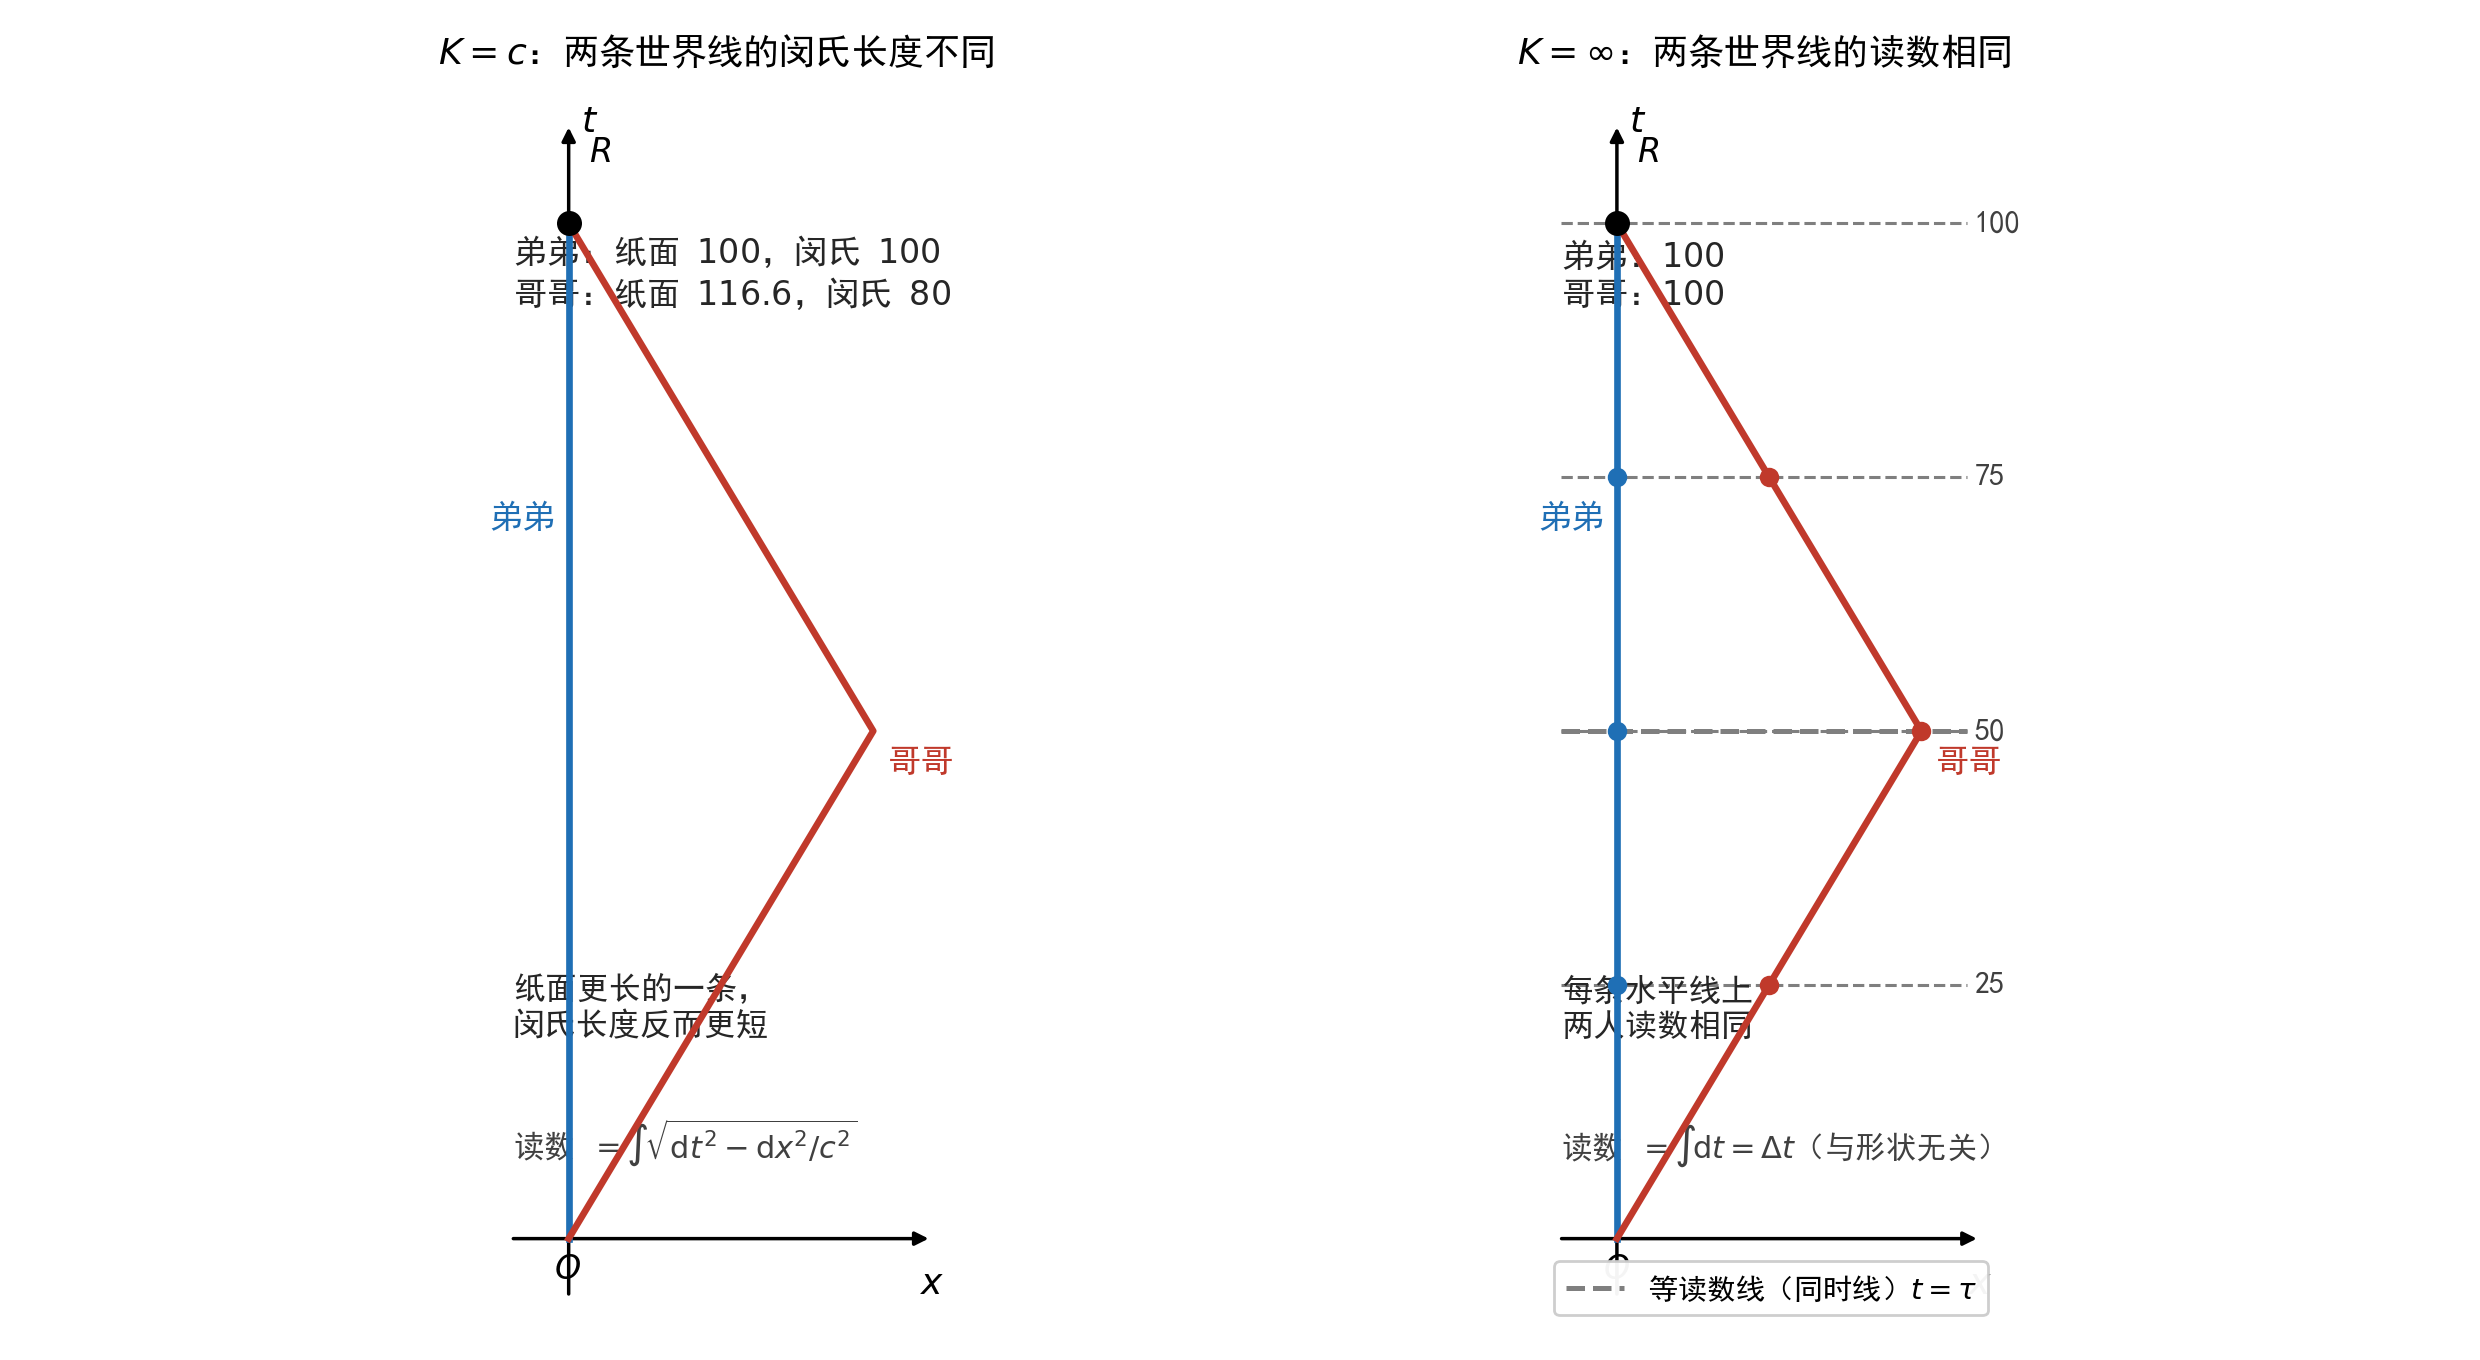
\includegraphics[width=1\linewidth,height=\textheight,keepaspectratio]{chapters/images/twins-earth-two-branches.png}

}

\caption{\label{fig-ta-two-branches}地球版双生子的两支对照：左为
\(K=c\)，两条世界线的闵氏长度不同；右为
\(K=\infty\)，等读数线变为水平直线，两条世界线读数相同}

\end{figure}%

左图中，弟弟的世界线纸面长 \(100\)、闵氏长 \(100\)；哥哥的折线纸面长
\(2\sqrt{50^{2}+30^{2}}=116.6\)、闵氏长
\(2\sqrt{50^{2}-30^{2}}=80\)------\textbf{纸面更长的一条，闵氏长度反而更短}。右图中，等读数线是水平直线
\(t=\tau\)，两条世界线被同一族水平线扫描，读数处处相同。

取 \(v=0.6c\)、\(d=30\) 光年、\(T=100\) 年，同一设定在两支下：

\begin{longtable}[]{@{}lll@{}}
\caption{同一设定在两支下的结果}\label{tbl-ta-numbers}\tabularnewline
\toprule\noalign{}
& \(K=c\) & \(K=\infty\) \\
\midrule\noalign{}
\endfirsthead
\toprule\noalign{}
& \(K=c\) & \(K=\infty\) \\
\midrule\noalign{}
\endhead
\bottomrule\noalign{}
\endlastfoot
弟弟读数 & \(100\) 年 & \(100\) 年 \\
哥哥读数 & \(100/\gamma=80\) 年 & \(100\) 年 \\
重逢读数差 & \(20\) 年 & \(0\) \\
读数是否依赖路径 & 依赖 & 不依赖 \\
钟慢因子 & \(\gamma=1.25\) & \(\gamma=1\) \\
\end{longtable}

\subsection{同时面与配对}\label{sec-ta-simultaneity}

两支的差别在几何上表现为同时面的形状：

\begin{itemize}
\tightlist
\item
  \textbf{\(K=c\)}：等固有读数轨迹是校准双曲线
  \(t^{2}-x^{2}/c^{2}=\tau^{2}\)（见
  小节~\ref{sec-tc-geometry}），同时面随参考系倾斜。
\item
  \textbf{\(K=\infty\)}：该双曲线变为水平直线
  \(t=\tau\)，与同时面重合，所有参考系共享。
\end{itemize}

表 表~\ref{tbl-tc-ratios} 中``对称与伽利略给出同一个数 \(1\)、洛伦兹给出
\(1/\gamma_w\)''这一点，在这一支里的对应说法是：对称判据所用的配对（起点相同
+ 过程对称 ⟹ 同时）是绝对同时的配对，正是 \(K=\infty\)
这一支的水平同时面；而 命题~\ref{prp-ta-equal}
表明，在这一支里该结论不需要对称这个前提。

（坐标非惯性时的处理，见第 章节~\ref{sec-twins-noninertial} 章。）

\subsection{适用域}\label{sec-ta-domain}

\begin{itemize}
\tightlist
\item
  \textbf{\(K=c\)}：变换的适用域为 \(v\le c\)。\(c\)
  是该结构的不变速度，同时是它的速度上界；超出时 \(\gamma\)
  出虚数，该结构不再适用。
\item
  \textbf{\(K=\infty\)}：变换 \(t'=t\)、\(x'=x-vt\) 对 \(v\)
  没有限制，\(v\) 取多大都成立。
\end{itemize}

\subsection{两支公设及其结果}\label{sec-ta-conclusion}

\begin{longtable}[]{@{}
  >{\raggedright\arraybackslash}p{(\linewidth - 4\tabcolsep) * \real{0.3333}}
  >{\raggedright\arraybackslash}p{(\linewidth - 4\tabcolsep) * \real{0.3333}}
  >{\raggedright\arraybackslash}p{(\linewidth - 4\tabcolsep) * \real{0.3333}}@{}}
\caption{两支公设及其结果}\label{tbl-ta-conclusion}\tabularnewline
\toprule\noalign{}
\begin{minipage}[b]{\linewidth}\raggedright
\end{minipage} & \begin{minipage}[b]{\linewidth}\raggedright
\(K=c\)
\end{minipage} & \begin{minipage}[b]{\linewidth}\raggedright
\(K=\infty\)
\end{minipage} \\
\midrule\noalign{}
\endfirsthead
\toprule\noalign{}
\begin{minipage}[b]{\linewidth}\raggedright
\end{minipage} & \begin{minipage}[b]{\linewidth}\raggedright
\(K=c\)
\end{minipage} & \begin{minipage}[b]{\linewidth}\raggedright
\(K=\infty\)
\end{minipage} \\
\midrule\noalign{}
\endhead
\bottomrule\noalign{}
\endlastfoot
不变速度 & 有限（\(c\)） & 无穷（不存在有限的不变速度） \\
时间坐标 & 随参考系改变 & 不随参考系改变 \\
读数尺度 & \(\mathrm{d}s^{2}=\mathrm{d}t^{2}-\mathrm{d}x^{2}/c^{2}\) &
\(\mathrm{d}s^{2}=\mathrm{d}t^{2}\) \\
同时面 & 随参考系倾斜 & 水平，所有系共享 \\
读数是否依赖路径 & 依赖 & 不依赖 \\
地球版双生子的读数 & \(\Delta\tau_D=T\)，\(\Delta\tau_G=T/\gamma\) &
\(\Delta\tau_D=\Delta\tau_G=T\) \\
适用域 & \(v\le c\) & 对 \(v\) 无限制 \\
\end{longtable}

\section{结论}\label{sec-tc-conclusion}

\begin{longtable}[]{@{}
  >{\raggedright\arraybackslash}p{(\linewidth - 2\tabcolsep) * \real{0.5000}}
  >{\raggedright\arraybackslash}p{(\linewidth - 2\tabcolsep) * \real{0.5000}}@{}}
\caption{各命题及其依据}\label{tbl-tc-conclusion}\tabularnewline
\toprule\noalign{}
\begin{minipage}[b]{\linewidth}\raggedright
命题
\end{minipage} & \begin{minipage}[b]{\linewidth}\raggedright
依据
\end{minipage} \\
\midrule\noalign{}
\endfirsthead
\toprule\noalign{}
\begin{minipage}[b]{\linewidth}\raggedright
命题
\end{minipage} & \begin{minipage}[b]{\linewidth}\raggedright
依据
\end{minipage} \\
\midrule\noalign{}
\endhead
\bottomrule\noalign{}
\endlastfoot
对称对上 \(\mathrm{d}\tau_B/\mathrm{d}\tau_A=1\) &
S1、S2、S3（命题~\ref{prp-tc-equal}） \\
A 本地读数即知 B 的读数 & 上一条的推论，不需要测量 \\
伽利略变换给出 \(\mathrm{d}\tau_B/\mathrm{d}\tau_A=1\) &
G1、G2（式~\ref{eq-tc-ratio-G}） \\
洛伦兹变换给出 \(\mathrm{d}\tau_B/\mathrm{d}\tau_A=1/\gamma_w\) &
L1、L2（式~\ref{eq-tc-ratio-L}） \\
只用洛伦兹变换推不出 \(\Delta\tau_A=\Delta\tau_B\) &
式~\ref{eq-tc-key} \\
只用伽利略变换能推出 \(\Delta\tau_A=\Delta\tau_B\) &
式~\ref{eq-tc-equal-G} \\
等固有读数点的轨迹是校准双曲线，不是欧氏圆 &
命题~\ref{prp-tc-hyperbola} \\
投影时 \(=\gamma_w\tau>\tau\)；投影差全部来自配对规则 &
推论~\ref{cor-tc-projection} \\
A 80 岁时 B 也 80 岁（对称）；A 的洛伦兹测量给 \(80/\gamma_w\)（配对） &
小节~\ref{sec-tc-lifespan} \\
地球视角中对称配对与同时配对重合；A、B 相互无钟慢 &
图~\ref{fig-tc-three-views} \\
\(K\to\infty\) 时双曲线变为水平线，各配对重合 &
小节~\ref{sec-tc-galilean-geometry}、表~\ref{tbl-tc-gamma} \\
地球版双生子：\(K=c\) 下 \(\Delta\tau_D=T\)、\(\Delta\tau_G=T/\gamma\) &
命题~\ref{prp-ta-lorentz-result} \\
地球版双生子：\(K=\infty\) 下 \(\Delta\tau_D=\Delta\tau_G=T\) &
命题~\ref{prp-ta-equal} \\
非惯性坐标下的线元与成立条件 & 第 章节~\ref{sec-twins-noninertial} 章 \\
\end{longtable}

\textbf{三个数：}

\[
\text{对称：}\ 1\qquad\qquad
\text{伽利略变换：}\ 1\qquad\qquad
\text{洛伦兹变换：}\ \frac{1}{\gamma_w}
\]

\bookmarksetup{startatroot}

\chapter{非惯性系下的对称双生子}\label{sec-twins-noninertial}

\section{本章的范围}\label{sec-tn-scope}

第 章节~\ref{sec-twins-comparison}
章的推导都在惯性坐标中进行。本章把坐标换成\textbf{沿曲线 A（或曲线
B）自身建立的坐标}------坐标非惯性------在 \(K=c\) 与 \(K=\infty\)
两支下分别画出 A 视角与 B
视角的时空图，并沿图上的像计算读数；最后沿三段结构（直线段---转向段---直线段）用校验线切割逐段比较两侧读数（小节~\ref{sec-tn-cut}）。

\textbf{输入清单}（全部是数学对象）：

{\def\LTcaptype{none} % do not increment counter
\begin{longtable}[]{@{}
  >{\raggedright\arraybackslash}p{(\linewidth - 4\tabcolsep) * \real{0.3333}}
  >{\raggedright\arraybackslash}p{(\linewidth - 4\tabcolsep) * \real{0.3333}}
  >{\raggedright\arraybackslash}p{(\linewidth - 4\tabcolsep) * \real{0.3333}}@{}}
\toprule\noalign{}
\begin{minipage}[b]{\linewidth}\raggedright
编号
\end{minipage} & \begin{minipage}[b]{\linewidth}\raggedright
对象
\end{minipage} & \begin{minipage}[b]{\linewidth}\raggedright
内容
\end{minipage} \\
\midrule\noalign{}
\endhead
\bottomrule\noalign{}
\endlastfoot
(M1) & 底空间与二次型 &
\(\mathrm{d}s^{2}_{K}=\mathrm{d}t^{2}-\mathrm{d}x^{2}/K^{2}\)，\(K=c\)
或 \(K=\infty\) \\
(M2) & 两条曲线 & \(\gamma_A\)、\(\gamma_B\)：从 \(O\) 到 \(M\)
的分段光滑类时曲线，每段或为直线段（曲率恒为零）或为曲线段（曲率不恒为零）；记号沿用：第一段
\(O\to P\)、\(O\to Q\)，末段
\(P\to M\)、\(Q\to M\)；小节~\ref{sec-tn-cut}
使用三段结构（直线段---转向段---直线段） \\
(M3) & 映射 \(\iota\) &
\(\iota(t,x)=(t,-x)\)；\(\iota(\gamma_A)=\gamma_B\)，\(\iota(O)=O\)，\(\iota(M)=M\) \\
(M4) & 读数定义 &
\(s[\gamma]=\displaystyle\int_{\gamma}\sqrt{\mathrm{d}t^{2}-\mathrm{d}x^{2}/K^{2}}\) \\
\end{longtable}
}

\textbf{两条纪律}：

\begin{enumerate}
\def\labelenumi{\arabic{enumi}.}
\tightlist
\item
  \textbf{不引入第三个坐标系}。全程只出现 A 视角坐标与 B
  视角坐标；\(K=c\)
  支中两系之间的变换是洛伦兹变换（它本身只连接两个坐标系）。
\item
  \textbf{\(\iota\) 只作几何输入}。(M3)
  定义了曲线对的镜像关系；本章不在任何计算步骤中用``因为镜像，所以读数相等''来替代或改动计算。所有读数都由积分算出；镜像能推出什么，由
  命题~\ref{prp-tn-isometry} 的证明给出。
\end{enumerate}

\textbf{不使用的内容}：本章不引用任何实验、不引入任何物理机制、不使用任何物理直觉；所有结论由代数与积分给出。

\section{数学准备}\label{sec-tn-math}

\subsection{镜像映射保持二次型}\label{ux955cux50cfux6620ux5c04ux4fddux6301ux4e8cux6b21ux578b}

\begin{proposition}[\(\iota\) 保持
\(\mathrm{d}s^{2}_{K}\)]\protect\hypertarget{prp-tn-isometry}{}\label{prp-tn-isometry}

对 \(K=c\) 与 \(K=\infty\)，\(\iota(t,x)=(t,-x)\) 满足
\(\iota^{*}\mathrm{d}s^{2}_{K}=\mathrm{d}s^{2}_{K}\)。

\end{proposition}

\textbf{证明}：\(\iota^{*}\mathrm{d}t=\mathrm{d}t\)，\(\iota^{*}\mathrm{d}x=-\mathrm{d}x\)，故
\(\iota^{*}\mathrm{d}s^{2}_{K}=\mathrm{d}t^{2}-(-\mathrm{d}x)^{2}/K^{2}=\mathrm{d}s^{2}_{K}\)。

\begin{corollary}[两条曲线的读数相等]\protect\hypertarget{cor-tn-length}{}\label{cor-tn-length}

\(s[\gamma_B]=s[\gamma_A]\)，对 \(K=c\) 与 \(K=\infty\) 都成立。

\end{corollary}

\textbf{证明}：曲线在等距映射下的长度不变（换元
\(y=\iota(x)\)，被积式与积分域都被 \(\iota\)
保形搬移，积分值不变）。\(\gamma_B=\iota(\gamma_A)\)，故
\(s[\gamma_B]=s[\gamma_A]\)。

推论~\ref{cor-tn-length} 是 (M3) 与 (M4)
的直接推论，全程未使用任何变换公式。它给出\textbf{整段读数}（从 \(O\) 到
\(M\)）的关系。本章其余部分把读数\textbf{分段、分视角}地算出来，并检查图上的像。

\subsection{两支的变换与读数因子}\label{ux4e24ux652fux7684ux53d8ux6362ux4e0eux8bfbux6570ux56e0ux5b50}

\(K=c\) 支中，相对速率 \(w\) 的两个坐标系之间：

\begin{equation}\protect\phantomsection\label{eq-tn-lorentz}{
t'=\gamma_w\Bigl(t-\frac{u\,x}{c^{2}}\Bigr),\qquad x'=\gamma_u(x-ut),\qquad
\gamma_u=\frac{1}{\sqrt{1-u^{2}/c^{2}}}
}\end{equation}

\(K=\infty\) 支中：

\begin{equation}\protect\phantomsection\label{eq-tn-galilei}{
t'=t,\qquad x'=x-ut
}\end{equation}

两支合起来可写为 \(\gamma_u(K)=1/\sqrt{1-u^{2}/K^{2}}\)：\(K=c\)
时即洛伦兹因子，\(K=\infty\) 时 \(\gamma_u(\infty)=1\)。

\section{A 视角坐标的构造}\label{sec-tn-construct}

设曲线 \(\gamma_A\) 以弧长参数（读数）\(\tau\) 描写，其一维情形下由快度
\(\theta(\tau)\) 给出（\(\mathrm{d}\theta/\mathrm{d}\tau=a(\tau)\)
为曲率，直线上 \(a=0\)）。\textbf{A 视角坐标}定义为

\begin{equation}\protect\phantomsection\label{eq-tn-fermi}{
t=T(\tau)+x_A\sinh\theta(\tau),\qquad
x=X(\tau)+x_A\cosh\theta(\tau),
}\end{equation}

其中
\(T(\tau)=\int_0^{\tau}\cosh\theta(u)\,\mathrm{d}u\)，\(X(\tau)=\int_0^{\tau}\sinh\theta(u)\,\mathrm{d}u\)。几何意义：从
\(\gamma_A\) 上参数为 \(\tau\) 的点出发，沿该点的正交单位方向移动距离
\(x_A\)。\(\gamma_A\) 在此坐标中是 \(x_A=0\)，且
\(t_A=\tau_A\)（纵轴即参数本身）。

\begin{proposition}[A
视角坐标中的线元（\(K=c\)）]\protect\hypertarget{prp-tn-metric}{}\label{prp-tn-metric}

\begin{equation}\protect\phantomsection\label{eq-tn-metric-c}{
\mathrm{d}s^{2}=\bigl(1+a(\tau)\,x_A\bigr)^{2}\,\mathrm{d}\tau^{2}-\mathrm{d}x_A^{2}
}\end{equation}

\end{proposition}

\textbf{证明}：对 式~\ref{eq-tn-fermi}
求偏导：\(\partial_\tau T=(1+a x_A)\cosh\theta\)，\(\partial_{x_A}T=\sinh\theta\)，\(\partial_\tau X=(1+a x_A)\sinh\theta\)，\(\partial_{x_A}X=\cosh\theta\)。代入
\(\mathrm{d}t^{2}-\mathrm{d}x^{2}\)，用
\(\cosh^{2}\theta-\sinh^{2}\theta=1\) 逐项化简即得。该式对任意
\(a(\tau)\) \textbf{精确成立}，不是近似。

\begin{proposition}[A
视角坐标中的线元（\(K=\infty\)）]\protect\hypertarget{prp-tn-metric-inf}{}\label{prp-tn-metric-inf}

\begin{equation}\protect\phantomsection\label{eq-tn-metric-inf}{
\mathrm{d}s^{2}=\mathrm{d}\tau^{2}
}\end{equation}

\end{proposition}

\textbf{证明}：\(K=\infty\) 支的变换 式~\ref{eq-tn-galilei} 中 \(t\)
不变，取 A 视角坐标 \(t_A=t\)、\(x_A=x-X(t)\)（沿 \(\gamma_A\)
的横移），代入 \(\mathrm{d}s^{2}=\mathrm{d}t^{2}\) 得
\(\mathrm{d}s^{2}=\mathrm{d}t_A^{2}\)；加速轨迹 \(X(t)\)
不出现在结果中。

两式并排：

\begin{longtable}[]{@{}
  >{\raggedright\arraybackslash}p{(\linewidth - 4\tabcolsep) * \real{0.3333}}
  >{\raggedright\arraybackslash}p{(\linewidth - 4\tabcolsep) * \real{0.3333}}
  >{\raggedright\arraybackslash}p{(\linewidth - 4\tabcolsep) * \real{0.3333}}@{}}
\caption{A 视角线元的两支对照}\label{tbl-tn-metric}\tabularnewline
\toprule\noalign{}
\begin{minipage}[b]{\linewidth}\raggedright
\end{minipage} & \begin{minipage}[b]{\linewidth}\raggedright
\(K=c\)
\end{minipage} & \begin{minipage}[b]{\linewidth}\raggedright
\(K=\infty\)
\end{minipage} \\
\midrule\noalign{}
\endfirsthead
\toprule\noalign{}
\begin{minipage}[b]{\linewidth}\raggedright
\end{minipage} & \begin{minipage}[b]{\linewidth}\raggedright
\(K=c\)
\end{minipage} & \begin{minipage}[b]{\linewidth}\raggedright
\(K=\infty\)
\end{minipage} \\
\midrule\noalign{}
\endhead
\bottomrule\noalign{}
\endlastfoot
A 视角线元 &
\(\bigl(1+a(\tau)x_A\bigr)^{2}\mathrm{d}\tau^{2}-\mathrm{d}x_A^{2}\) &
\(\mathrm{d}\tau^{2}\) \\
线元是否含 \(x_A\) & 含（\(a\neq0\) 时） & 不含 \\
曲率 \(a(\tau)\) 是否进入线元 & 进入 & 不进入 \\
\end{longtable}

\begin{figure}

\centering{

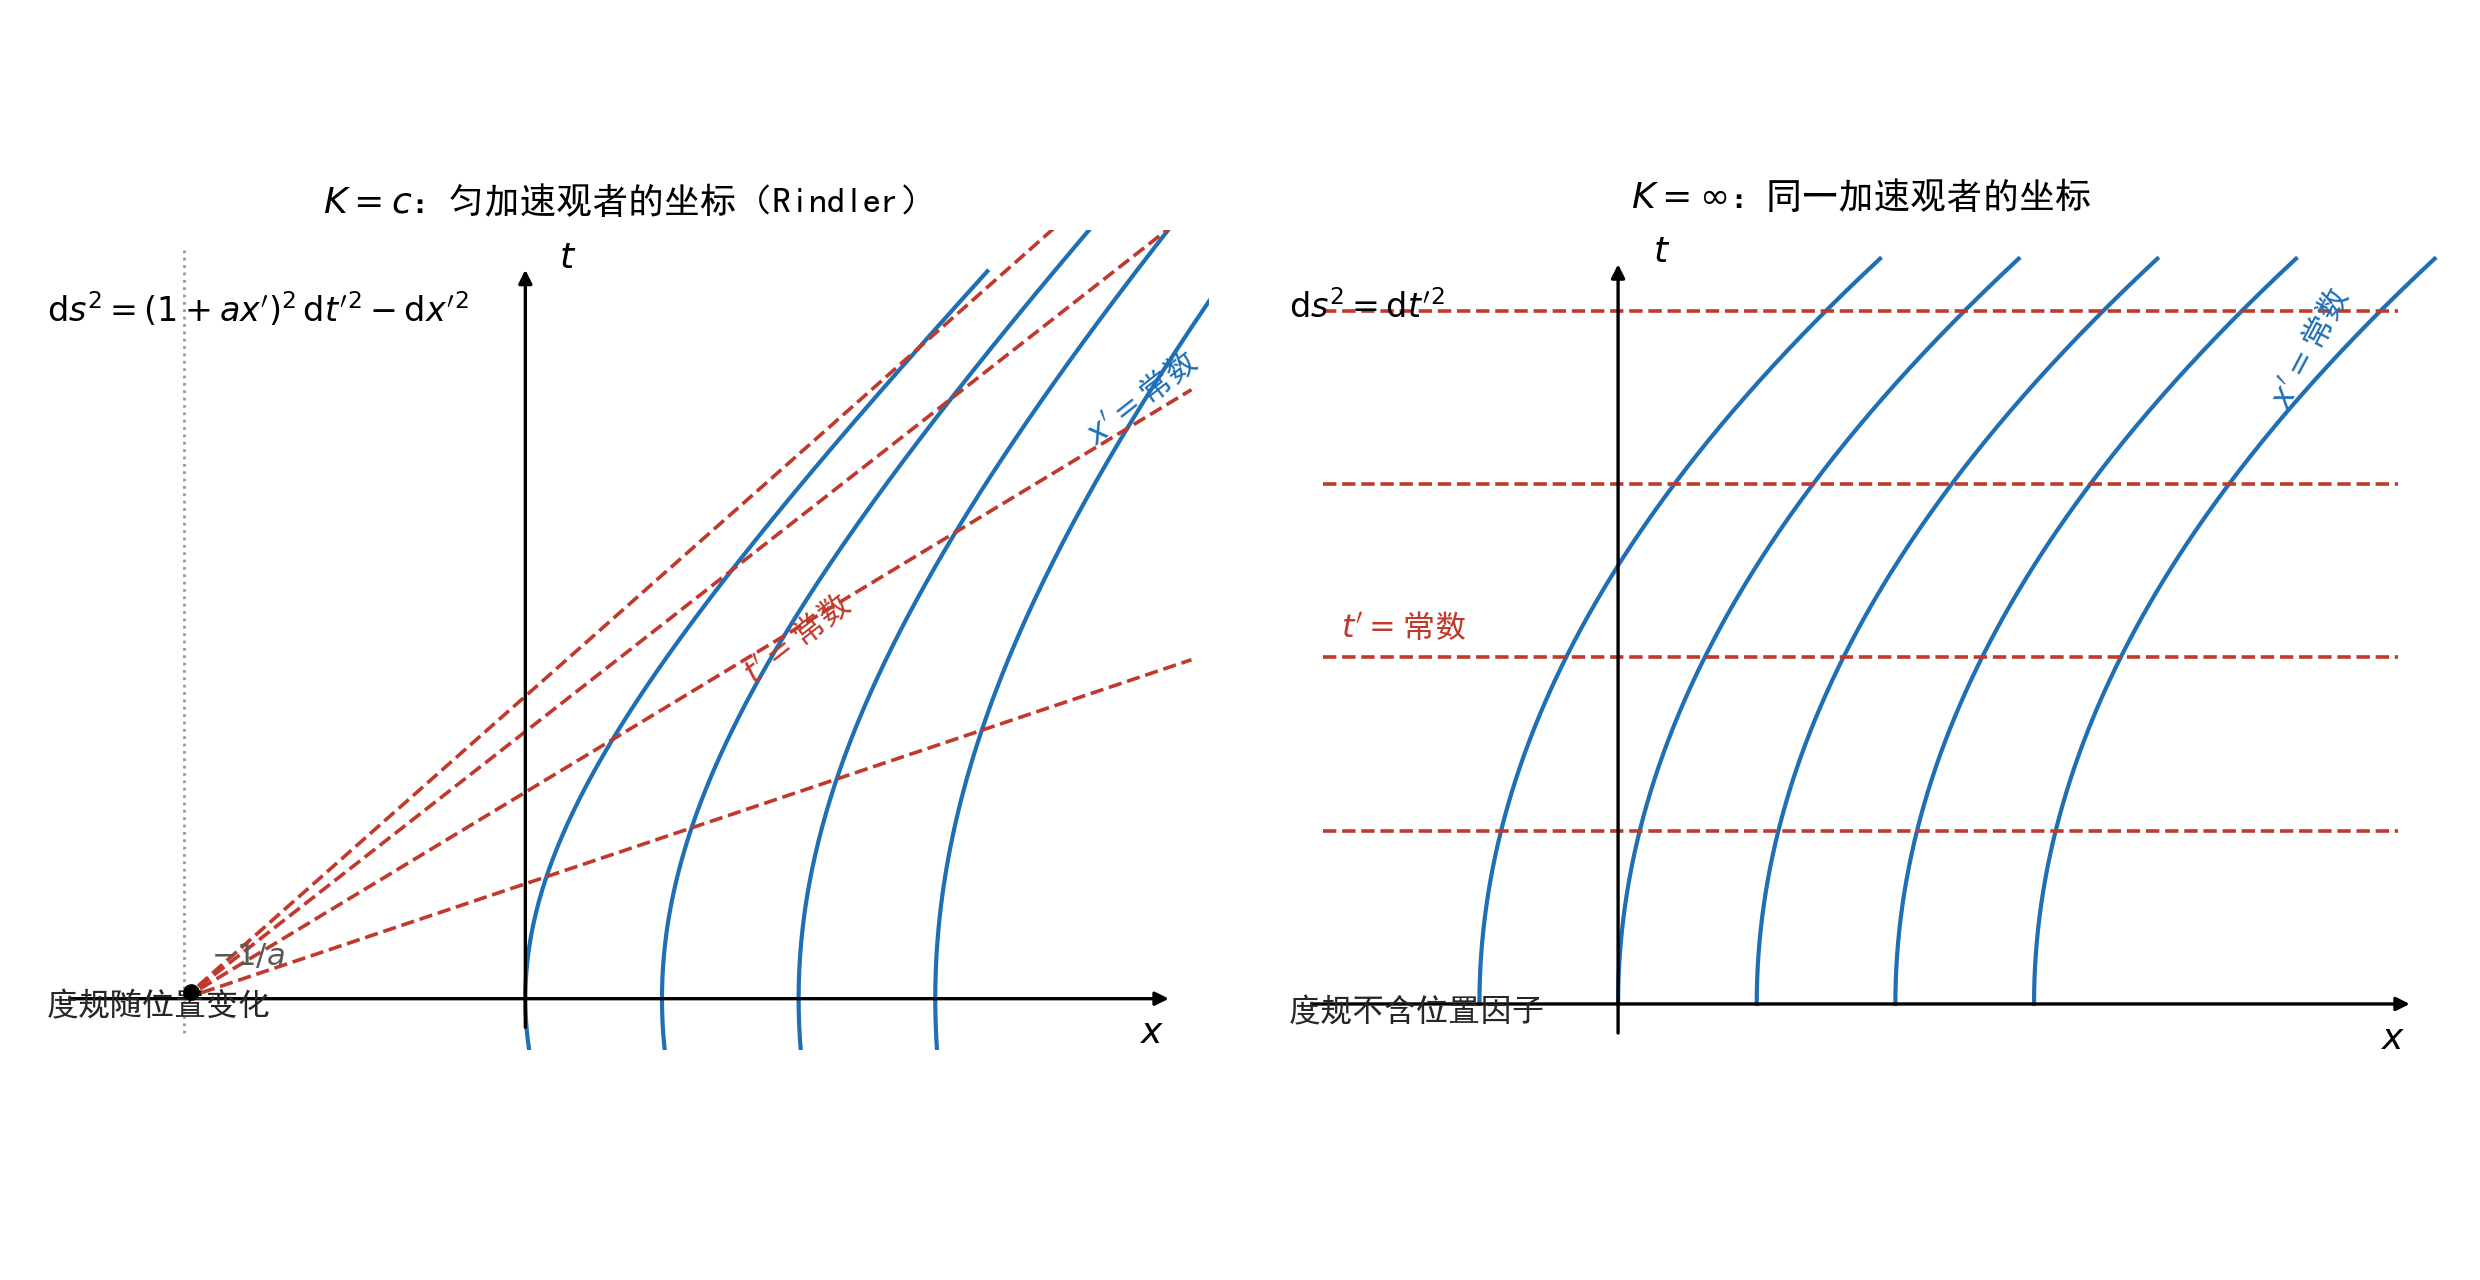
\includegraphics[width=1\linewidth,height=\textheight,keepaspectratio]{chapters/images/twins-noninertial-compare.png}

}

\caption{\label{fig-tn-compare}A 视角坐标画在 \((t,x)\) 平面上：左为
\(K=c\) 支，\(x_A=\)常数 是双曲线，\(t_A=\)常数 是过 \((-c^{2}/a,0)\)
的直线，线元随位置改变；右为 \(K=\infty\) 支，线元不变，\(t_A=\)常数
仍是水平线}

\end{figure}%

\section{坐标映射为单射的条件}\label{sec-tn-injective}

一张视角图要能画，坐标映射 \((\tau,x_A)\mapsto(t,x)\)
须在该处一一对应。两支的条件不同。

\begin{proposition}[\(K=c\)
支的单射条件]\protect\hypertarget{prp-tn-domain}{}\label{prp-tn-domain}

映射 式~\ref{eq-tn-fermi} 在点 \((\tau,x_A)\) 附近一一对应，当且仅当

\begin{equation}\protect\phantomsection\label{eq-tn-condition-c}{
1+\frac{a(\tau)\,x_A}{c^{2}}>0 .
}\end{equation}

\end{proposition}

\textbf{证明}：\(g_{\tau\tau}=(1+a x_A/c^{2})^{2}\) 在 \(x_A=-c^{2}/a\)
处为零。几何上，\(t_A=\text{常数}\) 的线在 \((t,x)\) 平面中是直线
\(t=\bigl(x+c^{2}/a\bigr)\tanh(a t_A/c)\)（\(a\)
为常数时），它们\textbf{全部过点}
\((-c^{2}/a,\,0)\)。该点是这族直线的公共交点：越过它，不同的
\((\tau,x_A)\) 对应同一事件，映射不再一一对应。公共交点位于 \(\gamma_A\)
的曲率反方向、距离 \(c^{2}/a\) 处。

\begin{proposition}[\(K=\infty\)
支的单射条件]\protect\hypertarget{prp-tn-domain-inf}{}\label{prp-tn-domain-inf}

映射 \(t_A=t\)、\(x_A=x-X(t)\) 的雅可比行列式为 \(1\)，处处非零；条件
式~\ref{eq-tn-condition-c} 在该支\textbf{没有对应的限制}，映射在全体
\((t,x)\) 上一一对应。

\end{proposition}

\textbf{证明}：\(\partial(t_A,x_A)/\partial(t,x)=\det\begin{pmatrix}1&0\\-X'(t)&1\end{pmatrix}=1\)。

\section{\texorpdfstring{\(K=c\) 支：对称双生子的 A 视角与 B
视角}{K=c 支：对称双生子的 A 视角与 B 视角}}\label{sec-tn-lorentz}

\subsection{直线段：两视角的读数计算}\label{ux76f4ux7ebfux6bb5ux4e24ux89c6ux89d2ux7684ux8bfbux6570ux8ba1ux7b97}

直线段上 \(a=0\)，线元为
\(\mathrm{d}s^{2}=\mathrm{d}t^{2}-\mathrm{d}x^{2}/c^{2}\)，坐标映射处处单射。设
A、B 的相对速率为 \(w\)（两坐标系之间由 式~\ref{eq-tn-lorentz}
直接连接）。

\textbf{A
视角}。取直线段起点为原点。\(\gamma_A\)：\(x_A=0\)；\(\gamma_B\)：\(x_A=-w\,t_A\)。

沿 \(\gamma_B\) 取读数增量为 \(\mathrm{d}\tau_B\) 的两个相邻事件，用
式~\ref{eq-tn-lorentz} 换到 A 坐标（B
在自己的坐标中位置不变，\(\mathrm{d}x_B=0\)）：

\begin{equation}\protect\phantomsection\label{eq-tn-ratio-A}{
\mathrm{d}t_A=\gamma_w\,\mathrm{d}\tau_B
\qquad\Longrightarrow\qquad
\boxed{\ \mathrm{d}\tau_B=\frac{\mathrm{d}t_A}{\gamma_w}\ }
}\end{equation}

\textbf{B 视角}。同一计算，A 与 B
互换（\(\gamma_B\)：\(x_B=0\)；\(\gamma_A\)：\(x_B=+w\,t_B\)；换算时
\(w\to-w\)，\(\gamma_w\) 不变）：

\begin{equation}\protect\phantomsection\label{eq-tn-ratio-B}{
\boxed{\ \mathrm{d}\tau_A=\frac{\mathrm{d}t_B}{\gamma_w}\ }
}\end{equation}

式~\ref{eq-tn-ratio-A} 与 式~\ref{eq-tn-ratio-B}
是\textbf{两个独立的计算}：前者把 \(\gamma_B\) 上的事件对换到 A
坐标，后者把 \(\gamma_A\) 上的事件对换到 B
坐标；两组事件对不同，两个关系式分别成立，二者之间没有矛盾。两个式子互为镜像（把
A、B 互换即得对方）------这一条由 式~\ref{eq-tn-lorentz} 在 \(u\to-u\)
下的不变性给出，是计算的性质，不是外加的假设。

\textbf{图上的两条线}（图~\ref{fig-tn-views} 上行）：

\begin{itemize}
\tightlist
\item
  \textbf{等读数线}：从原点出发、以任意恒定速率运动的曲线，读数为
  \(\tau\) 的事件满足 \(t^{2}-x^{2}/c^{2}=\tau^{2}\)（把 \(u=x/t\)
  代入读数式即得）。\(\gamma_A\) 上读 \(\tau\) 的事件 \((\tau,0)\) 与
  \(\gamma_B\) 上读 \(\tau\) 的事件 \((\gamma_w\tau,-w\gamma_w\tau)\)
  在同一条曲线上。
\item
  \textbf{本系同时线}：\(t_A=\text{常数}\)，水平线。过 \((\tau,0)\)
  的水平线与 \(\gamma_B\) 交于 \(t_A=\tau\) 处，由
  式~\ref{eq-tn-ratio-A} 该点的 B 读数为 \(\tau/\gamma_w\)。
\end{itemize}

\subsection{弧线段：像的定义域}\label{ux5f27ux7ebfux6bb5ux50cfux7684ux5b9aux4e49ux57df}

弧线段上 \(a\neq0\)，A 视角坐标的线元由 式~\ref{eq-tn-metric-c}
给出，单射条件由 命题~\ref{prp-tn-domain}
给出。取解析可解的镜像曲线对------\(\gamma_A\) 以固定曲率 \(+a\)
弯曲、\(\gamma_B\) 以 \(-a\) 镜像弯曲（\(c=1\)）------求 \(\gamma_B\) 在
A 视角坐标中的像。

\(\gamma_B\) 上参数为 \(u=a\tau_A\) 的事件在 A 视角坐标中满足（记
\(\rho=1+x_A\)）：

\[
\rho\sinh(a\tau')=\sinh u,\qquad \rho\cosh(a\tau')=2-\cosh u,
\]

两式平方相减消去 \(\tau'\)：

\begin{equation}\protect\phantomsection\label{eq-tn-rho}{
\rho^{2}=5-4\cosh u .
}\end{equation}

实像存在当且仅当 \(\rho^{2}>0\)：

\begin{equation}\protect\phantomsection\label{eq-tn-ln2}{
\cosh u<\frac54
\qquad\Longleftrightarrow\qquad
u<\operatorname{arccosh}\tfrac54=\ln 2 .
}\end{equation}

\begin{corollary}[镜像弯曲曲线对的像区间]\protect\hypertarget{cor-tn-domain-ln2}{}\label{cor-tn-domain-ln2}

\(K=c\) 支中，A 视角坐标里 \(\gamma_B\) 的像存在的条件是

\[
a\,\tau_A<\ln 2\approx0.693 .
\]

临界处 \(\rho=\sqrt{5-4\cosh(\ln 2)}=0\)，即
\(x_A=-c^{2}/a\)：\(\gamma_B\) 的像恰好到达 式~\ref{eq-tn-condition-c}
的边界。\(a\tau_A\geq\ln2\)
时该处\textbf{没有实像}------图上该段无法表示 \(\gamma_B\)。

\end{corollary}

\begin{figure}

\centering{

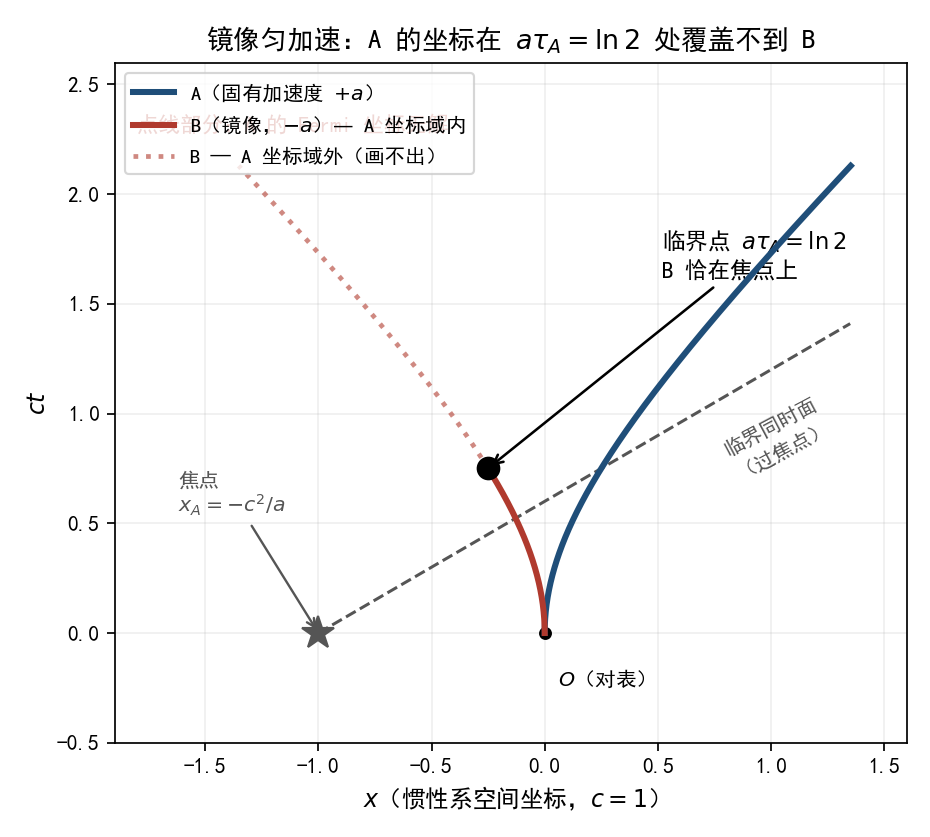
\includegraphics[width=0.82\linewidth,height=\textheight,keepaspectratio]{chapters/images/twins-noninertial-domain.png}

}

\caption{\label{fig-tn-domain}\(K=c\) 支：镜像弯曲曲线对中 \(\gamma_B\)
在 A 视角坐标中的像。\(a\tau_A<\ln2\) 时像存在；临界处像到达
\(x_A=-c^{2}/a\)；其后（点线）没有实像}

\end{figure}%

\textbf{数值标度}（\(c=1\) 时 \(a\tau\) 无量纲；恢复 \(c\) 后
\(\tau_A<(c/a)\ln2\)）：

\begin{longtable}[]{@{}lll@{}}
\caption{\(K=c\) 支像区间的数值标度}\label{tbl-tn-scale}\tabularnewline
\toprule\noalign{}
\(a\) & \(c^{2}/a\) & \(\tau_A^{*}=(c/a)\ln2\) \\
\midrule\noalign{}
\endfirsthead
\toprule\noalign{}
\(a\) & \(c^{2}/a\) & \(\tau_A^{*}=(c/a)\ln2\) \\
\midrule\noalign{}
\endhead
\bottomrule\noalign{}
\endlastfoot
\(9.8\,\mathrm{m/s^{2}}\) & \(0.97\) 光年 & \(0.67\) 年 \\
\(0.98\,\mathrm{m/s^{2}}\) & \(9.7\) 光年 & \(6.7\) 年 \\
\(0.098\,\mathrm{m/s^{2}}\) & \(97\) 光年 & \(67\) 年 \\
\end{longtable}

\subsection{B 视角}\label{b-ux89c6ux89d2}

B 视角坐标由同一个构造沿 \(\gamma_B\) 建立。命题~\ref{prp-tn-isometry}
的镜像映射把 \((\gamma_A,a,+x)\) 换为 \((\gamma_B,a,-x)\)，故
式~\ref{eq-tn-rho}、推论~\ref{cor-tn-domain-ln2} 与
表~\ref{tbl-tn-scale} 对 B 视角\textbf{逐字成立}（把 \(x_A\) 换为
\(x_B\)、\(\gamma_A\) 换为 \(\gamma_B\)）------这一条由 \(\iota\)
保形搬移全部等式给出，是代数性质。

\subsection{整段读数}\label{ux6574ux6bb5ux8bfbux6570}

由
推论~\ref{cor-tn-length}：\(s[\gamma_A]=s[\gamma_B]\)。分段看：直线段上
A 视角与 B
视角各自的计算（式~\ref{eq-tn-ratio-A}、式~\ref{eq-tn-ratio-B}）给出的是\textbf{对方读数与本系坐标时的关系}，不是整段读数的比较；整段读数由积分
式~\ref{eq-tn-rho} 所属的同一套线元沿两条曲线分别积分，其相等由
推论~\ref{cor-tn-length} 保证。

\section{\texorpdfstring{\(K=\infty\) 支：对称双生子的 A 视角与 B
视角}{K=\textbackslash infty 支：对称双生子的 A 视角与 B 视角}}\label{sec-tn-galilean}

\subsection{线元与像}\label{ux7ebfux5143ux4e0eux50cf}

A 视角线元为
\(\mathrm{d}s^{2}=\mathrm{d}\tau^{2}\)（命题~\ref{prp-tn-metric-inf}），坐标映射处处单射（命题~\ref{prp-tn-domain-inf}）。\(\gamma_B\)
在 A 视角坐标中的像：设 \(\gamma_B\) 为 \(x=\xi(t)\)，则像为

\begin{equation}\protect\phantomsection\label{eq-tn-image-inf}{
t_A=t,\qquad x_A=\xi(t)-X(t),
}\end{equation}

对任意 \(\xi\) 存在，无定义域限制。沿像的读数：

\begin{equation}\protect\phantomsection\label{eq-tn-read-inf}{
\mathrm{d}\tau_B=\mathrm{d}t_A
\qquad\Longrightarrow\qquad
s[\gamma_B]=t_A(M)-t_A(O).
}\end{equation}

右端只含端点的 \(t_A\) 坐标，与 \(\xi\) 的形状无关。\(\gamma_A\)
同理：\(s[\gamma_A]=t_A(M)-t_A(O)\)。

\subsection{B 视角}\label{b-ux89c6ux89d2-1}

同一构造沿 \(\gamma_B\) 建立：\(t_B=t\)，\(x_B=x-\Xi(t)\)（\(\Xi\) 为
\(\gamma_B\) 的轨迹）。雅可比同样恒为 \(1\)，线元同样为
\(\mathrm{d}s^{2}=\mathrm{d}t_B^{2}\)，读数同样只由端点给出。A 视角与 B
视角的两个时间坐标相等（式~\ref{eq-tn-galilei}
的第一式），故两视角给出同一个数。

\subsection{\texorpdfstring{图（图~\ref{fig-tn-views}
下行）}{图（图~ 下行）}}\label{ux56fefig-tn-views-ux4e0bux884c}

\(K=\infty\) 支的等读数线与同时线重合，都是水平直线 \(t=\tau\)；A 视角与
B 视角互为镜像，两条曲线上的等读数点落在同一条水平线上。

\section{校验线切割：惯性段的读数贡献}\label{sec-tn-cut}

前两节分别给出了每支里两视角各自的计算。本节回到
(M1)---(M4)，回答一个更细的问题：把两条曲线分成对应的段，逐段比较两侧读数，\textbf{差从哪些段来}。本节只使用
(M1)---(M4) 已有的坐标描述与映射 \(\iota\)，不引入新的坐标系。

\subsection{三段结构}\label{ux4e09ux6bb5ux7ed3ux6784}

\textbf{结构假设 (S)}：\(\gamma_A\)、\(\gamma_B\) 各由三段组成------段
I：从 \(O\) 出发的直线段；段 II：曲率不恒为零的转向段；段 III：到达
\(M\) 的直线段。

由 命题~\ref{prp-tn-isometry}，\(\iota\)
保持二次型，因而保持曲线的曲率。\(\gamma_B=\iota(\gamma_A)\) 时，把
\(\gamma_A\) 按曲率分段，\(\gamma_B\) 的对应分段由 \(\iota\)
直接给出：\(\iota\) 把 \(\gamma_A\) 的段 I、II、III 分别映为
\(\gamma_B\) 的段 I、II、III。这不是附加假设，是 (M3) 的推论。

\subsection{校验线}\label{ux6821ux9a8cux7ebf}

\begin{definition}[校验线]\protect\hypertarget{def-tn-calibration}{}\label{def-tn-calibration}

\(K=c\) 支中，以 \(O\) 为心、参数 \(\tau\) 的校验线与以 \(M\) 为心、参数
\(\sigma\) 的校验线为

\begin{equation}\protect\phantomsection\label{eq-tn-calibration}{
\Lambda_O(\tau)=\bigl\{X:\ t^{2}-x^{2}/c^{2}=\tau^{2},\ t>0\bigr\},
}\end{equation}

\begin{equation}\protect\phantomsection\label{eq-tn-calibration-m}{
\Lambda_M(\sigma)=\bigl\{X:\ (t_M-t)^{2}-(x-x_M)^{2}/c^{2}=\sigma^{2},\ t<t_M\bigr\}.
}\end{equation}

\(K=\infty\) 支中，校验线为 \(t=t_O+\tau\) 与 \(t=t_M-\sigma\)。

\end{definition}

\(K=c\) 支的校验线即 图~\ref{fig-tn-views}
中的等读数线（\(t^{2}-x^{2}/c^{2}=\tau^{2}\)），也就是第
章节~\ref{sec-twins-comparison}
章的\textbf{校准双曲线}（式~\ref{eq-tc-hyperbola}）：落在
\(\Lambda_O(\tau)\) 上当且仅当该事件由 \(O\) 出发的读数为
\(\tau\)。本节把它用作切割工具。\(K=\infty\)
支的校验线是水平线（等读数线与同时线重合，见
小节~\ref{sec-tn-galilean}）。

\begin{proposition}[校准引理]\protect\hypertarget{prp-tn-calibration}{}\label{prp-tn-calibration}

\(K=c\) 支中，设事件 \(X\) 由 \(O\) 出发沿直线段（任意恒定速率
\(|u|<c\)）到达，读数为 \(s\)，则 \(s^{2}=t(X)^{2}-x(X)^{2}/c^{2}\)，即
\(X\in\Lambda_O(s)\)，\textbf{与速率 \(u\) 无关}。\(K=\infty\) 支中，从
\(O\) 出发到 \(X\) 的读数为
\(t(X)-t(O)\)，与路径形状无关，同一校验线上每点的读数相同。

\end{proposition}

\textbf{证明}：直线 \(x=ut\)
上，\(s=\displaystyle\int_{0}^{t(X)}\sqrt{1-u^{2}/c^{2}}\,\mathrm{d}t'=t(X)\sqrt{1-u^{2}/c^{2}}\)，而
\(t(X)^{2}-x(X)^{2}/c^{2}=t(X)^{2}\bigl(1-u^{2}/c^{2}\bigr)=s^{2}\)。\(K=\infty\)
支即 式~\ref{eq-tn-read-inf} 的直接读出。

引理的要点是\textbf{与速率无关}：两个以不同恒定速率从 \(O\)
出发的人，跨过同一条 \(\Lambda_O(\tau)\) 时读数同为
\(\tau\)（数值核验：\(u=0.1,0.6,0.9,0.99\) 的直线跨
\(\Lambda_O(0.4)\)，读数均为 \(0.4\)）。

\subsection{分段定理}\label{ux5206ux6bb5ux5b9aux7406}

沿每条曲线，段 I 上的读数从 \(0\)（在 \(O\)）起严格递增，段 III
上的读数到 \(M\) 止严格递增。故当 \(\tau_1\) 小于段 I
的读数、\(\sigma_1\) 小于段 III 的读数时，\(\Lambda_O(\tau_1)\) 与段 I
有唯一交点，\(\Lambda_M(\sigma_1)\) 与段 III
有唯一交点------由校准引理，交点即读数为 \(\tau_1\)、\(\sigma_1\)
的事件。称这样的 \(\tau_1,\sigma_1\) 为\textbf{容许切割}。

\begin{theorem}[分段定理]\protect\hypertarget{thm-tn-cut}{}\label{thm-tn-cut}

取容许切割 \(\tau_1,\sigma_1\)，记段 I 与 \(\Lambda_O(\tau_1)\) 的交点为
\(E_A,E_B\)，段 III 与 \(\Lambda_M(\sigma_1)\) 的交点为 \(F_A,F_B\)。则

\begin{enumerate}
\def\labelenumi{\arabic{enumi}.}
\tightlist
\item
  \(s[O\to E_A]=s[O\to E_B]=\tau_1\)；
\item
  \(s[F_A\to M]=s[F_B\to M]=\sigma_1\)；
\item
  \(s[E_A\to F_A]=s[E_B\to F_B]\)；
\item
  \(s[\gamma_A]=s[\gamma_B]=\tau_1+s[E_A\to F_A]+\sigma_1\)；
\item
  结论 1、2、4 对一切容许切割成立，与 \(\tau_1,\sigma_1\) 的取值无关。
\end{enumerate}

\end{theorem}

\textbf{证明}：

\begin{enumerate}
\def\labelenumi{\arabic{enumi}.}
\tightlist
\item
  段 I 上读数为 \(\tau_1\) 的事件由校准引理落在 \(\Lambda_O(\tau_1)\)
  上，读数严格递增给出唯一性；A、B 两侧同一论证。
\item
  把校准引理用于以 \(M\) 为心、时间反向的校验线，同一论证。
\item
  \(\iota\) 保持 \(t^{2}-x^{2}/c^{2}\) 与
  \(t\)（命题~\ref{prp-tn-isometry} 的计算），故
  \(\iota\bigl(\Lambda_O(\tau_1)\bigr)=\Lambda_O(\tau_1)\)、\(\iota\bigl(\Lambda_M(\sigma_1)\bigr)=\Lambda_M(\sigma_1)\)，且
  \(\iota\) 把 \(\gamma_A\) 的段 I、III 分别映为 \(\gamma_B\) 的段
  I、III。交点唯一给出 \(\iota(E_A)=E_B\)、\(\iota(F_A)=F_B\)；\(\iota\)
  保持线元，子段的读数不变（推论~\ref{cor-tn-length}
  的同一论证用于子段）。
\item
  三段相加，用 1、2、3。
\item
  1、2 的论证对每个容许 \(\tau_1,\sigma_1\) 逐字重复；4 由 1、2、3
  相加。
\end{enumerate}

注：结论 1、2
只用了校准引理，没有用到镜像性------即使两条惯性段的速率不同，1、2
仍成立；镜像性只在结论 3（中间段）处进入。

\begin{corollary}[惯性段的贡献]\protect\hypertarget{cor-tn-legs}{}\label{cor-tn-legs}

段 I 与段 III 对两侧总读数之差的贡献为
\(0\)；此贡献与切割位置无关（定理~\ref{thm-tn-cut} 第 5
条），与两段上的速率取值无关（校准引理）。两侧读数的全部共同部分由中间段给出，而中间段两侧读数相等（定理~\ref{thm-tn-cut}
第 3 条）。

\end{corollary}

\subsection{显式算例}\label{ux663eux5f0fux7b97ux4f8b}

取 \(c=1\)，\(O=(0,0)\)，\(M=(4,0)\)：

\begin{equation}\protect\phantomsection\label{eq-tn-example}{
\gamma_A:\quad
x(t)=\begin{cases}
-0.6\,t, & 0\le t\le 1,\\[2pt]
0.3\,t^{2}-1.2\,t+0.3, & 1\le t\le 3,\\[2pt]
0.6\,t-2.4, & 3\le t\le 4,
\end{cases}
}\end{equation}

其中 \(\gamma_B:\ x(t)=-x_A(t)\)。

逐项检查：三段在 \(t=1,3\) 处位置连续（值 \(-0.6\)）且速率连续（从
\(-0.6\) 变到
\(+0.6\)）；\(|\mathrm{d}x/\mathrm{d}t|\le 0.6<1\)，全程类时；段 II
的切线方向连续变化，曲率不恒为零，确为转向段。\(\gamma_B\) 与
\(\gamma_A\) 同起于 \(O\)、同终于 \(M\)，互为镜像。

\begin{longtable}[]{@{}
  >{\raggedright\arraybackslash}p{(\linewidth - 4\tabcolsep) * \real{0.3333}}
  >{\raggedright\arraybackslash}p{(\linewidth - 4\tabcolsep) * \real{0.3333}}
  >{\raggedright\arraybackslash}p{(\linewidth - 4\tabcolsep) * \real{0.3333}}@{}}
\caption{算例的三段读数}\label{tbl-tn-example}\tabularnewline
\toprule\noalign{}
\begin{minipage}[b]{\linewidth}\raggedright
段
\end{minipage} & \begin{minipage}[b]{\linewidth}\raggedright
读数（闭式）
\end{minipage} & \begin{minipage}[b]{\linewidth}\raggedright
数值
\end{minipage} \\
\midrule\noalign{}
\endfirsthead
\toprule\noalign{}
\begin{minipage}[b]{\linewidth}\raggedright
段
\end{minipage} & \begin{minipage}[b]{\linewidth}\raggedright
读数（闭式）
\end{minipage} & \begin{minipage}[b]{\linewidth}\raggedright
数值
\end{minipage} \\
\midrule\noalign{}
\endhead
\bottomrule\noalign{}
\endlastfoot
段 I（惯性） & \(0.8\) & \(0.8\) \\
段 II（转向） & \(\sqrt{1-0.6^{2}}+\arcsin(0.6)/0.6\) &
\(1.8725018\ldots\) \\
段 III（惯性） & \(0.8\) & \(0.8\) \\
总读数 & & \(3.4725018\ldots\) \\
\end{longtable}

A、B 两侧逐段相同（镜像）。

切割：取
\(\tau_1=\sigma_1=0.4\)。\(E_A=(0.5,-0.3)\)、\(E_B=(0.5,0.3)\)：核对
\(0.5^{2}-0.3^{2}=0.16=0.4^{2}\)；\(F_A=(3.5,-0.3)\)、\(F_B=(3.5,0.3)\)：核对
\((4-3.5)^{2}-0.3^{2}=0.16\)。中间段读数为
\(3.4725-0.4-0.4=2.6725\)，两侧相同。把 \(\tau_1,\sigma_1\) 换为
\(0.2,0.6,0.8\) 逐项重算，段 I、段 III 两侧之差在每种取法下均为
\(0\)。以上数值由符号计算与高精度积分逐项核验。

\begin{figure}

\centering{

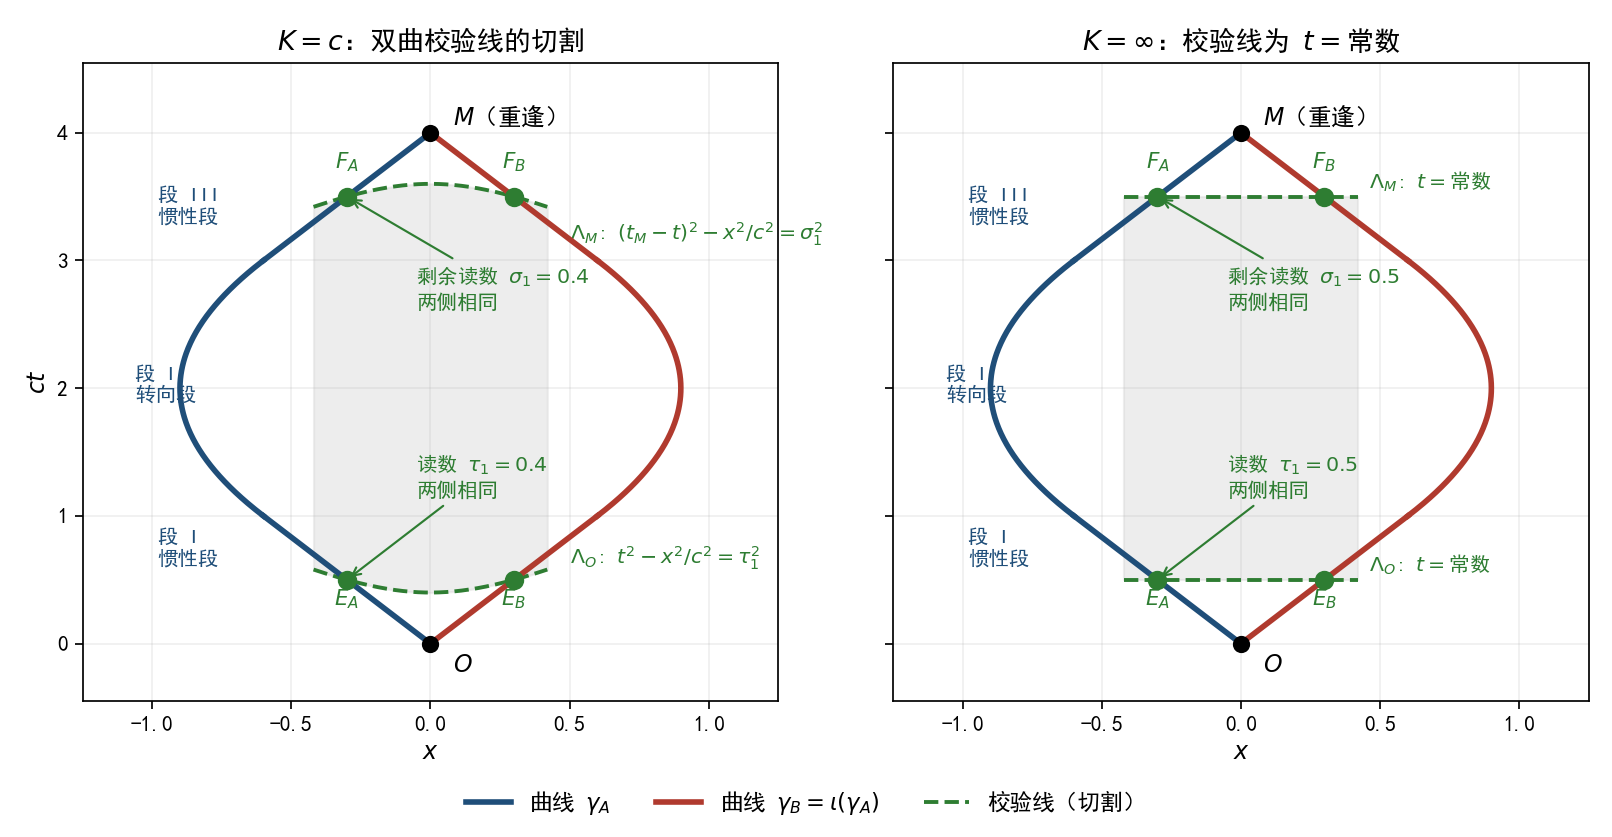
\includegraphics[width=1\linewidth,height=\textheight,keepaspectratio]{chapters/images/twins-calibration-cut.png}

}

\caption{\label{fig-tn-cut}对称双生子的三段结构与校验线切割。左：\(K=c\)，切割线为以
\(O\)、\(M\)
为心的双曲校验线；右：\(K=\infty\)，切割线为水平线（该支读数即 \(t\)
之差，同一切点的读数值相应为 \(0.5\)）。\(E_A,E_B\) 与 \(F_A,F_B\)
处两侧读数相同}

\end{figure}%

\subsection{与同时面配对的关系}\label{ux4e0eux540cux65f6ux9762ux914dux5bf9ux7684ux5173ux7cfb}

式~\ref{eq-tn-ratio-A} 与 式~\ref{eq-tn-ratio-B}
用的是\textbf{本系同时线}配出的事件对：把 \(\gamma_B\) 上的事件与
\(\gamma_A\) 坐标时相同的事件配对，读出因子
\(1/\gamma_w\)。本节的校验线用的是\textbf{另一种事件对}：把两条曲线上读数相同的事件配对（定理~\ref{thm-tn-cut}
第 1、2 条），读出 \(1\)。

两套事件对不同，两个结论分别成立，不相互矛盾；它们都是关于\textbf{配对}的陈述。总读数不经任何配对：由
(M4) 沿曲线积分给出，定理~\ref{thm-tn-cut} 第 4 条给出两侧相等、第 5
条给出与切割位置无关。

又：本节的切割只用到两条曲线上的事件与 \(\iota\)，不需要把 \(\gamma_B\)
表示到 A 自己的视角坐标里，故 推论~\ref{cor-tn-domain-ln2}
的像区间限制不涉及本节的结论。

\subsection{物理诠释}\label{ux7269ux7406ux8be0ux91ca}

以下诠释不引入新的数学对象，只复述已证结果在本章结构 (S) 中的含义。

\textbf{在对称双生子实验中，惯性运动部分不会造成任何实质性的时间变慢。}
依据是 推论~\ref{cor-tn-legs}：两段惯性段对读数之差的贡献恒等于
\(0\)，与切割位置无关、与速率无关。

\begin{enumerate}
\def\labelenumi{\arabic{enumi}.}
\tightlist
\item
  两条互为镜像的曲线，重逢时读数相同（推论~\ref{cor-tn-length}）；分段看，差只能来自中间段，而中间段两侧读数相等（定理~\ref{thm-tn-cut}
  第 3 条）。
\item
  ``变慢''的因子随配对的出现而出现、随配对的更换而消失：用某一方自己的同时面配对，读出
  \(1/\gamma_w\)（式~\ref{eq-tn-ratio-A}、式~\ref{eq-tn-ratio-B}）；用校验线配对，读出
  \(1\)（定理~\ref{thm-tn-cut}）。因子的取值是配对的属性；曲线的读数------(M4)
  的积分------不是配对的属性，它不随配对改变。
\item
  转向段在这一实验中也不构成两侧的差异：两侧读数相等由镜像等距给出（定理~\ref{thm-tn-cut}
  第 3 条）。
\end{enumerate}

\section{两支对照}\label{sec-tn-compare}

\begin{longtable}[]{@{}
  >{\raggedright\arraybackslash}p{(\linewidth - 4\tabcolsep) * \real{0.3333}}
  >{\raggedright\arraybackslash}p{(\linewidth - 4\tabcolsep) * \real{0.3333}}
  >{\raggedright\arraybackslash}p{(\linewidth - 4\tabcolsep) * \real{0.3333}}@{}}
\caption{两支对照}\label{tbl-tn-summary}\tabularnewline
\toprule\noalign{}
\begin{minipage}[b]{\linewidth}\raggedright
\end{minipage} & \begin{minipage}[b]{\linewidth}\raggedright
\(K=c\)
\end{minipage} & \begin{minipage}[b]{\linewidth}\raggedright
\(K=\infty\)
\end{minipage} \\
\midrule\noalign{}
\endfirsthead
\toprule\noalign{}
\begin{minipage}[b]{\linewidth}\raggedright
\end{minipage} & \begin{minipage}[b]{\linewidth}\raggedright
\(K=c\)
\end{minipage} & \begin{minipage}[b]{\linewidth}\raggedright
\(K=\infty\)
\end{minipage} \\
\midrule\noalign{}
\endhead
\bottomrule\noalign{}
\endlastfoot
A 视角线元 &
\(\bigl(1+a(\tau)x_A\bigr)^{2}\mathrm{d}\tau^{2}-\mathrm{d}x_A^{2}\) &
\(\mathrm{d}\tau^{2}\) \\
直线段：对方读数与本系坐标时 &
\(\mathrm{d}\tau_B=\mathrm{d}t_A/\gamma_w\)（A
视角）；\(\mathrm{d}\tau_A=\mathrm{d}t_B/\gamma_w\)（B 视角） &
\(\mathrm{d}\tau_B=\mathrm{d}t_A\)；\(\mathrm{d}\tau_A=\mathrm{d}t_B\) \\
弧线段：坐标映射单射条件 & \(1+a x_A/c^{2}>0\) & 恒成立（雅可比
\(=1\)） \\
弧线段：\(\gamma_B\) 在 A 视角中的像 & 存在当且仅当
\(a\tau_A<\ln2\)（镜像弯曲曲线对） & 处处存在 \\
校验线切割后的惯性段读数 & 两侧相同（定理~\ref{thm-tn-cut}） &
两侧相同（定理~\ref{thm-tn-cut}） \\
整段读数 & \(s[\gamma_A]=s[\gamma_B]\) &
\(s[\gamma_A]=s[\gamma_B]\)，且都等于端点 \(t\) 之差 \\
\end{longtable}

\begin{figure}

\centering{

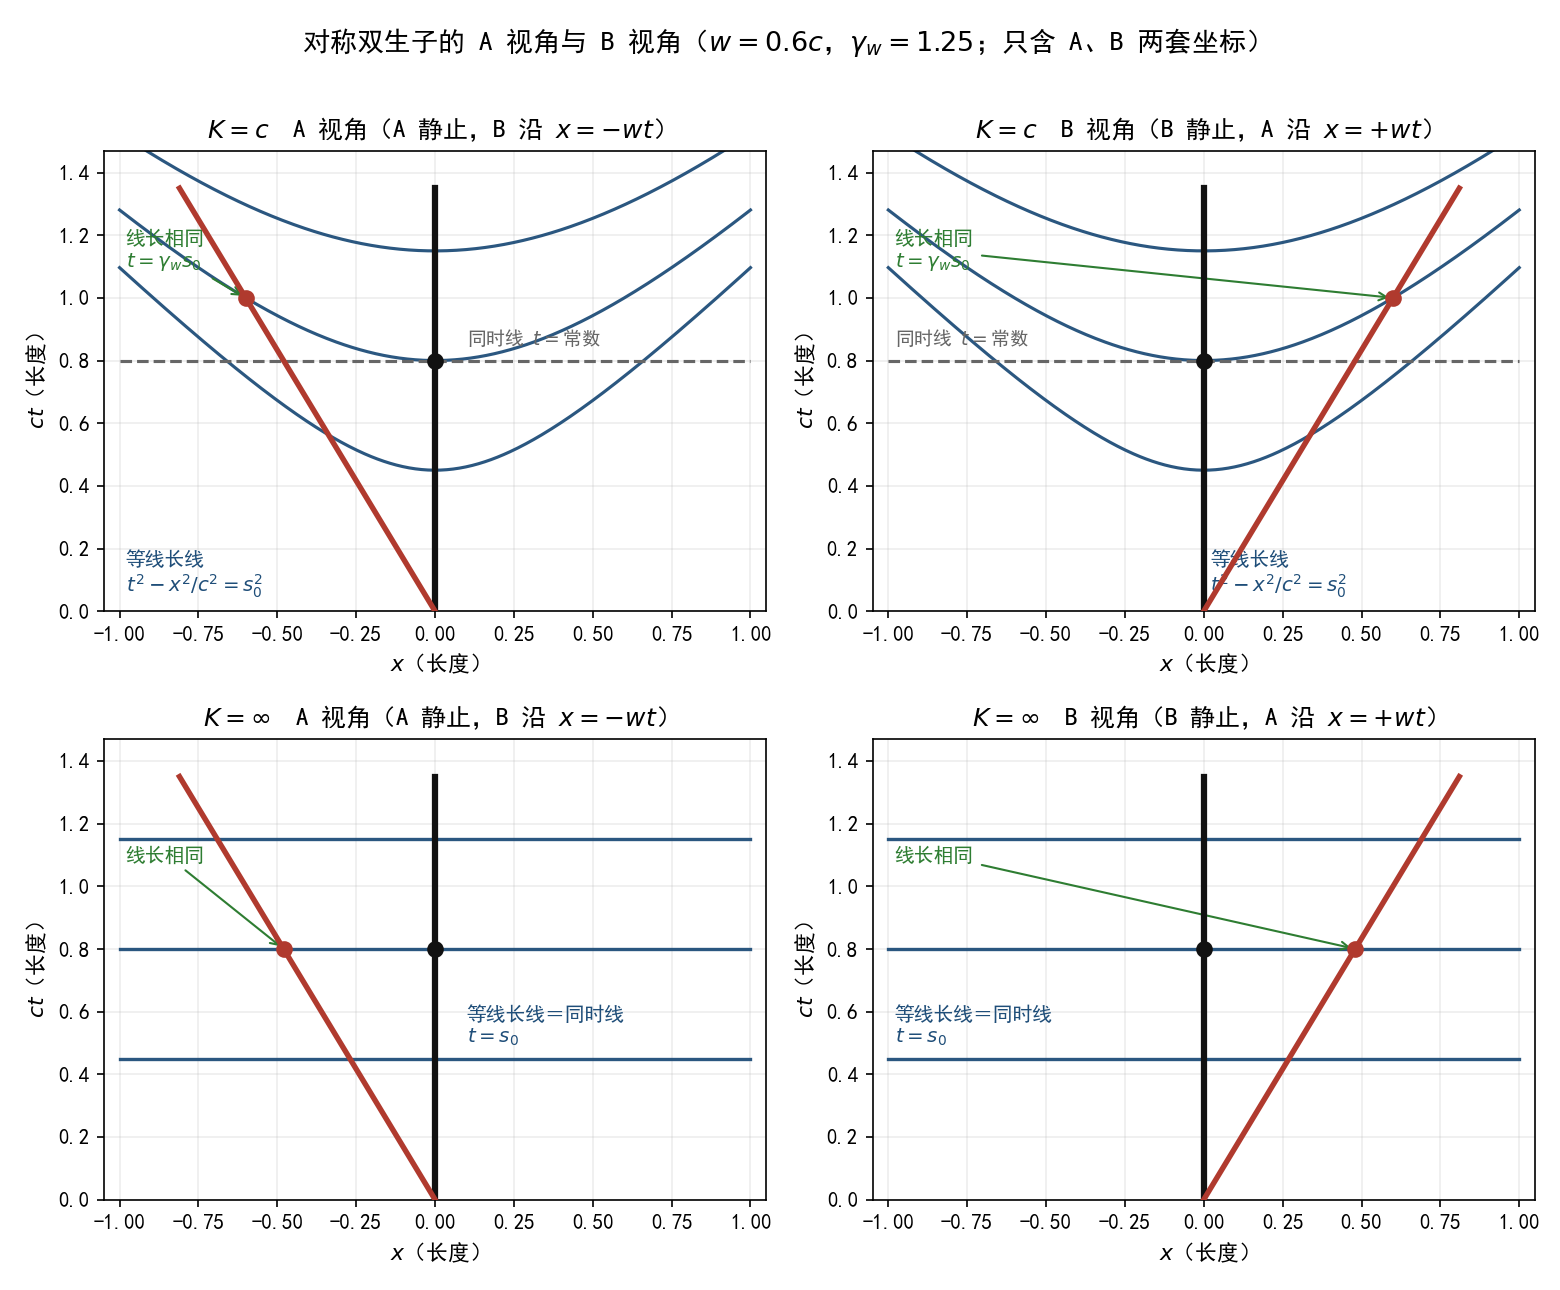
\includegraphics[width=1\linewidth,height=\textheight,keepaspectratio]{chapters/images/twins-ab-views.png}

}

\caption{\label{fig-tn-views}A 视角与 B
视角（\(w=0.6c\)，\(\gamma_w=1.25\)；每个面板只含所画视角的坐标与两条曲线）。上行
\(K=c\)：等读数线为
\(t^{2}-x^{2}/c^{2}=\tau^{2}\)，本系同时线为水平线，两线不同；下行
\(K=\infty\)：等读数线与同时线重合，均为 \(t=\tau\)。两支中 B 视角都是 A
视角的镜像}

\end{figure}%

\section{结果}\label{sec-tn-results}

本章推导得出的结果，逐条列出：

\begin{enumerate}
\def\labelenumi{\arabic{enumi}.}
\tightlist
\item
  \textbf{镜像映射保持读数}（命题~\ref{prp-tn-isometry}、推论~\ref{cor-tn-length}）：\(s[\gamma_A]=s[\gamma_B]\)，两支都成立。依据是
  \(\iota\) 保二次型与曲线长度在等距映射下不变，未使用任何变换公式。
\item
  \textbf{\(K=c\)
  支，直线段}（式~\ref{eq-tn-ratio-A}、式~\ref{eq-tn-ratio-B}）：A
  视角算得 \(\mathrm{d}\tau_B=\mathrm{d}t_A/\gamma_w\)；B 视角算得
  \(\mathrm{d}\tau_A=\mathrm{d}t_B/\gamma_w\)。两式互为镜像，分别关于不同的事件对。
\item
  \textbf{\(K=c\)
  支，弧线段}（命题~\ref{prp-tn-metric}、命题~\ref{prp-tn-domain}、推论~\ref{cor-tn-domain-ln2}）：A
  视角线元为
  \(\bigl(1+a x_A/c^{2}\bigr)^{2}\mathrm{d}\tau^{2}-\mathrm{d}x_A^{2}\)；坐标映射的单射条件为
  \(1+a x_A/c^{2}>0\)；镜像弯曲曲线对中 \(\gamma_B\) 的像存在当且仅当
  \(a\tau_A<\ln2\)，临界处像到达 \(x_A=-c^{2}/a\)，其后没有实像。B
  视角逐字相同。
\item
  \textbf{\(K=\infty\)
  支}（命题~\ref{prp-tn-metric-inf}、命题~\ref{prp-tn-domain-inf}、式~\ref{eq-tn-read-inf}）：A
  视角线元为
  \(\mathrm{d}\tau^{2}\)，加速轨迹不进入；坐标映射处处单射；\(\gamma_B\)
  的像处处存在；读数只由端点的 \(t\) 坐标给出，与路径形状无关。B
  视角相同。
\item
  \textbf{对比}（表~\ref{tbl-tn-summary}、图~\ref{fig-tn-views}）：两支的差别集中在弧线段------\(K=c\)
  支的 A 视角（及 B 视角）坐标对另一条曲线的像有区间限制，\(K=\infty\)
  支没有；直线段上，\(K=c\) 支的两视角各给出一个 \(1/\gamma_w\)
  因子，\(K=\infty\) 支给出 \(1\)。
\item
  \textbf{分段与配对}（命题~\ref{prp-tn-calibration}、定理~\ref{thm-tn-cut}、推论~\ref{cor-tn-legs}）：以
  \(O\)、\(M\)
  为心的校验线切割三段结构后，两段惯性段对读数之差的贡献恒为
  \(0\)------与切割位置无关、与速率无关；中间段两侧读数相等；总读数
  \(s[\gamma_A]=s[\gamma_B]\) 与切割位置无关。\(1/\gamma_w\)
  因子与本节的 \(1\) 是两套配对各自的结果（见 小节~\ref{sec-tn-cut}
  ``与同时面配对的关系''一节）。
\end{enumerate}

\bookmarksetup{startatroot}

\chapter*{符号与约定}\label{sec-notation}
\addcontentsline{toc}{chapter}{符号与约定}

\markboth{符号与约定}{符号与约定}

本书跨十三章、涉及群论、微分几何、量子力学与场论，同一个字母在不同章可能承担不同角色。本表登记全书主要符号及其角色，供查阅。

\section*{时空、坐标与指标}\label{sec-notation-coords}
\addcontentsline{toc}{section}{时空、坐标与指标}

\markright{时空、坐标与指标}

{\def\LTcaptype{none} % do not increment counter
\begin{longtable}[]{@{}
  >{\raggedright\arraybackslash}p{(\linewidth - 4\tabcolsep) * \real{0.3333}}
  >{\raggedright\arraybackslash}p{(\linewidth - 4\tabcolsep) * \real{0.3333}}
  >{\raggedright\arraybackslash}p{(\linewidth - 4\tabcolsep) * \real{0.3333}}@{}}
\toprule\noalign{}
\begin{minipage}[b]{\linewidth}\raggedright
符号
\end{minipage} & \begin{minipage}[b]{\linewidth}\raggedright
含义
\end{minipage} & \begin{minipage}[b]{\linewidth}\raggedright
主要出处
\end{minipage} \\
\midrule\noalign{}
\endhead
\bottomrule\noalign{}
\endlastfoot
\((t,x^{i})\)、\((t,x)\) & 时间坐标与空间坐标（第 13 章用 \((t,x)\)
平面） & 全书 \\
\(M\) & 时空流形 & 第 4---6、11 章 \\
\(\mu,\nu,\rho,\sigma\) & 四维时空指标，取值 \(0,1,2,3\) & 第 4---6、11
章 \\
\(i,j,k\) & 三维空间指标，取值 \(1,2,3\) & 第 4---6、11 章 \\
\(\partial_{\mu}\)、\(\partial_{t}\) &
偏导数；\(\partial_{0}\equiv\partial_{t}\) & 全书 \\
\(\mathbf{x},\mathbf{v},\mathbf{k}\) & 三维欧氏向量（粗体） & 第 7---9
章 \\
\(\eta_{\mu\nu}\) & 闵氏度规；第 5、11 章用作\textbf{固定背景}张量 & 第
5、11 章 \\
\(g_{\mu\nu}\) & 时空度规 & 第 4---6、11 章 \\
\end{longtable}
}

\textbf{约定}：指标由所在章指定的度规升降（第 11 章明确用 \(\eta\)
升降）；\(\partial_{\mu}\) 与 \(\partial_{0}\) 在同一章内不混用。

\section*{恒速场与恒速群}\label{sec-notation-K}
\addcontentsline{toc}{section}{恒速场与恒速群}

\markright{恒速场与恒速群}

{\def\LTcaptype{none} % do not increment counter
\begin{longtable}[]{@{}
  >{\raggedright\arraybackslash}p{(\linewidth - 4\tabcolsep) * \real{0.3333}}
  >{\raggedright\arraybackslash}p{(\linewidth - 4\tabcolsep) * \real{0.3333}}
  >{\raggedright\arraybackslash}p{(\linewidth - 4\tabcolsep) * \real{0.3333}}@{}}
\toprule\noalign{}
\begin{minipage}[b]{\linewidth}\raggedright
符号
\end{minipage} & \begin{minipage}[b]{\linewidth}\raggedright
含义
\end{minipage} & \begin{minipage}[b]{\linewidth}\raggedright
主要出处
\end{minipage} \\
\midrule\noalign{}
\endhead
\bottomrule\noalign{}
\endlastfoot
\(K\) & \textbf{恒速场}，恒速群的参数；\(K=c\) 为洛伦兹支，\(K=\infty\)
为伽利略支，\(K=0\) 为 Carroll 极限 & 第 2---7、13 章 \\
\(G_{K}\) & 恒速群（参数 \(K\) 的李群族） & 第 3、7 章 \\
\(c\) & \(K\) 取有限值时的记号；\(c\) \textbf{不是}独立于 \(K\)
的常数，\(K=c\) 只是这一支的写法 & 第 2、3 章 \\
\(u\) & 坐标变换（boost）的变换速度参数 & 第 2、3 章 \\
\(v\) & 两系相对速度，或源相对介质的速度（按章在首次使用时说明） & 第
2、10 章 \\
\(w\) & 合成速度；第 13 章 \(w=\dfrac{2v}{1+v^{2}/c^{2}}\) & 第 13 章 \\
\(\gamma_{u}\) & \(\bigl(1-u^{2}/K^{2}\bigr)^{-1/2}\)；\(K=c\)
时为通常的 \(\gamma\) & 第 2、13 章 \\
\(\gamma_{w}\) & 第 13 章中 \(w\) 对应的因子
\(=\dfrac{1+v^{2}/c^{2}}{1-v^{2}/c^{2}}\) & 第 13 章 \\
\(\beta^{i}\)、\(h_{ij}\) & ADM 分解中的 shift 与空间度规 & 第 6 章 \\
\end{longtable}
}

\textbf{\(K\) 的三种出现（务必区分）}：

\begin{enumerate}
\def\labelenumi{\arabic{enumi}.}
\tightlist
\item
  \textbf{恒速场 / 群参数} ------ 全书的默认含义（第 2---7、13 章）。
\item
  \textbf{ADM 分解中的 lapse} ------ 第 6 章。该章明确取 lapse
  即恒速场，故与第 1 条是\textbf{同一对象}，不是符号冲突。
\item
  \textbf{约束算子} ------ 第 12 章曾用
  \(K:=A_{R}\otimes 1-1\otimes A_{C}\)，与恒速场无关；现改用
  \(\mathscr{C}\)，避免混淆。
\end{enumerate}

\textbf{定义域}：\(K\) 的参数空间取 \((0,\infty]\)；\(K=0\)（Carroll）与
\(K=\infty\)（伽利略）作为边界/极限点处理。第 6 章 Schwarzschild 视界处
\(K\to0\)，按退化边界理解，不作为 \(K\) 的正则取值。

\section*{读数、几何与曲率}\label{sec-notation-geometry}
\addcontentsline{toc}{section}{读数、几何与曲率}

\markright{读数、几何与曲率}

{\def\LTcaptype{none} % do not increment counter
\begin{longtable}[]{@{}
  >{\raggedright\arraybackslash}p{(\linewidth - 4\tabcolsep) * \real{0.3333}}
  >{\raggedright\arraybackslash}p{(\linewidth - 4\tabcolsep) * \real{0.3333}}
  >{\raggedright\arraybackslash}p{(\linewidth - 4\tabcolsep) * \real{0.3333}}@{}}
\toprule\noalign{}
\begin{minipage}[b]{\linewidth}\raggedright
符号
\end{minipage} & \begin{minipage}[b]{\linewidth}\raggedright
含义
\end{minipage} & \begin{minipage}[b]{\linewidth}\raggedright
主要出处
\end{minipage} \\
\midrule\noalign{}
\endhead
\bottomrule\noalign{}
\endlastfoot
\(\tau\) & 随身钟的读数（沿世界线累积） & 第 1、13 章 \\
\(\mathrm{d}s^{2}\) & 读数尺度；\(K=c\) 时
\(\mathrm{d}t^{2}-\mathrm{d}x^{2}/c^{2}\)，\(K=\infty\) 时退化为
\(\mathrm{d}t^{2}\) & 第 3、13 章 \\
\(\int\mathrm{d}s\) & 沿世界线的累积读数 & 第 13 章 \\
\(\iota\) & 镜像映射 \((t,x)\mapsto(t,-x)\) & 第 13 章 \\
\(R^{\mu}{}_{\nu\rho\sigma}\)、\(R_{\mu\nu}\)、\(R\) & 黎曼张量、Ricci
张量、Ricci 标量 & 第 4---6、11 章 \\
\(G_{\mu\nu}\) & Einstein 张量 \(R_{\mu\nu}-\tfrac12 g_{\mu\nu}R\) & 第
5、6、11 章 \\
\(C_{\mu\nu\rho\sigma}\) & Weyl 张量 & 第 6 章 \\
\(\kappa\) & 引力耦合常数；第 5 章取 \(\kappa=8\pi G/K_{0}^{4}\) & 第
5、6、11 章 \\
\end{longtable}
}

\textbf{曲率约定}（各章一致，由 \texttt{chapters/images/}
下的符号计算脚本按此式逐项给出）：

\[
R_{\mu\nu}
=\partial_{\rho}\Gamma^{\rho}_{\nu\mu}
-\partial_{\nu}\Gamma^{\rho}_{\rho\mu}
+\Gamma^{\rho}_{\rho\lambda}\Gamma^{\lambda}_{\nu\mu}
-\Gamma^{\rho}_{\nu\lambda}\Gamma^{\lambda}_{\rho\mu},
\qquad R=g^{\mu\nu}R_{\mu\nu}
\]

\section*{电磁场}\label{sec-notation-em}
\addcontentsline{toc}{section}{电磁场}

\markright{电磁场}

{\def\LTcaptype{none} % do not increment counter
\begin{longtable}[]{@{}lll@{}}
\toprule\noalign{}
符号 & 含义 & 主要出处 \\
\midrule\noalign{}
\endhead
\bottomrule\noalign{}
\endlastfoot
\(\mathbf{E},\mathbf{B}\) & 电场、磁场 & 第 8、9 章 \\
\(F_{\mu\nu}\) & 电磁场张量 & 第 8、9 章 \\
\(a\) & 第 9 章中待定的变换系数 & 第 9 章 \\
\end{longtable}
}

\section*{量子部分}\label{sec-notation-quantum}
\addcontentsline{toc}{section}{量子部分}

\markright{量子部分}

{\def\LTcaptype{none} % do not increment counter
\begin{longtable}[]{@{}
  >{\raggedright\arraybackslash}p{(\linewidth - 4\tabcolsep) * \real{0.3333}}
  >{\raggedright\arraybackslash}p{(\linewidth - 4\tabcolsep) * \real{0.3333}}
  >{\raggedright\arraybackslash}p{(\linewidth - 4\tabcolsep) * \real{0.3333}}@{}}
\toprule\noalign{}
\begin{minipage}[b]{\linewidth}\raggedright
符号
\end{minipage} & \begin{minipage}[b]{\linewidth}\raggedright
含义
\end{minipage} & \begin{minipage}[b]{\linewidth}\raggedright
主要出处
\end{minipage} \\
\midrule\noalign{}
\endhead
\bottomrule\noalign{}
\endlastfoot
\(\hbar\) & 约化普朗克常数 & 第 7、12 章 \\
\(\hat{X}\) & 算符（帽号） & 第 7、12 章 \\
\(m\) & 质量；第 7 章中作为\textbf{中央荷}出现（非 Casimir 本征值） & 第
7 章 \\
\(\hat{B}_{i},\hat{P}_{j},\hat{H}\) & boost、动量、哈密顿算符 & 第 7
章 \\
\(\xi(g_{2},g_{1})\) & 群 2-闭上链 & 第 7 章 \\
\end{longtable}
}

\textbf{\(\hbar\) 与 \(h\)}：\(\hbar\) 恒为约化普朗克常数；\(h\)
另有两种含义（见下），与 \(\hbar\) 无关。

\section*{第 11---12 章}\label{sec-notation-later}
\addcontentsline{toc}{section}{第 11---12 章}

\markright{第 11---12 章}

{\def\LTcaptype{none} % do not increment counter
\begin{longtable}[]{@{}
  >{\raggedright\arraybackslash}p{(\linewidth - 4\tabcolsep) * \real{0.3333}}
  >{\raggedright\arraybackslash}p{(\linewidth - 4\tabcolsep) * \real{0.3333}}
  >{\raggedright\arraybackslash}p{(\linewidth - 4\tabcolsep) * \real{0.3333}}@{}}
\toprule\noalign{}
\begin{minipage}[b]{\linewidth}\raggedright
符号
\end{minipage} & \begin{minipage}[b]{\linewidth}\raggedright
含义
\end{minipage} & \begin{minipage}[b]{\linewidth}\raggedright
主要出处
\end{minipage} \\
\midrule\noalign{}
\endhead
\bottomrule\noalign{}
\endlastfoot
\(h\)、\(h_{\mu\nu}\) & 度规扰动，\(g=\eta+h\)；第 12 章的 \(h_{i}\)
是\textbf{函数}（另一含义） & 第 11、12 章 \\
\(\Phi\) & 背景场（第 12 章中为\textbf{给定的自变量}，不由方程决定） &
第 10、12 章 \\
\(f_{i}\) & 第 \(i\) 类钟的速率函数 & 第 12 章 \\
\(X_{ij}=f_{i}/f_{j}\) & 两类钟的比值 & 第 12 章 \\
\(Q_{ij}\)、\(P_{i}\) & 两点比较量；\(Q_{ij}\) 落在 \(\mathscr{M}\)
上，\(P_{i}\) 依赖代表 & 第 12 章 \\
\(\mathscr{M}\) & 模空间（等价类空间） & 第 12 章 \\
\(\mathscr{C}\) & 约束算子 \(A_{R}\otimes 1-1\otimes A_{C}\) & 第 12
章 \\
\(E\)、\(E_{C}\) & POVM、时钟子系统的 POVM & 第 12 章 \\
\end{longtable}
}

\section*{双生子实验}\label{sec-notation-twins}
\addcontentsline{toc}{section}{双生子实验}

\markright{双生子实验}

{\def\LTcaptype{none} % do not increment counter
\begin{longtable}[]{@{}ll@{}}
\toprule\noalign{}
符号 & 含义 \\
\midrule\noalign{}
\endhead
\bottomrule\noalign{}
\endlastfoot
\(A\)、\(B\) & 两个对称的观者（第 1、13 章） \\
\(D\)、\(G\) & 地球版双生子中的弟弟、哥哥（第 13 章） \\
\(O\)、\(R\)、\(M\) & 分离事件、重逢事件、中间事件 \\
\(P\)、\(Q\) & 两条世界线上的对称点 \\
\(d\) & 单程距离；\(T=2d/v\) 为地球系全程 \\
\end{longtable}
}

\section*{体例约定}\label{sec-notation-style}
\addcontentsline{toc}{section}{体例约定}

\markright{体例约定}

\begin{enumerate}
\def\labelenumi{\arabic{enumi}.}
\tightlist
\item
  \textbf{定理类环境}：公理（\texttt{cnj}）、定义（\texttt{def}）、命题（\texttt{prp}）、定理（\texttt{thm}）、引理（\texttt{lem}）、推论（\texttt{cor}），按章连续编号。
\item
  \textbf{公式编号}按章连续；交叉引用使用超链接，不用手写式号。
\item
  \textbf{证明结束}不另加结束符号。
\item
  \textbf{计算来源}：各章闭式由 \texttt{chapters/images/}
  下的符号计算脚本给出，脚本与正文同源；改动公式须同步改动脚本。
\end{enumerate}

\bookmarksetup{startatroot}

\chapter*{参考文献}\label{ux53c2ux8003ux6587ux732e}
\addcontentsline{toc}{chapter}{参考文献}

\markboth{参考文献}{参考文献}

\protect\phantomsection\label{refs}
\begin{CSLReferences}{0}{0}
\bibitem[\citeproctext]{ref-einstein1905}
\CSLLeftMargin{{[}1{]} }%
\CSLRightInline{EINSTEIN A. Zur Elektrodynamik bewegter
K{ö}rper{[}J/OL{]}. Annalen der Physik, 1905, 322(10): 891-921.
DOI:\href{https://doi.org/10.1002/andp.19053221004}{10.1002/andp.19053221004}.}

\bibitem[\citeproctext]{ref-levyleblond1976}
\CSLLeftMargin{{[}2{]} }%
\CSLRightInline{LÉVY-LEBLOND J M. One more derivation of the Lorentz
transformation{[}J/OL{]}. American Journal of Physics, 1976, 44(3):
271-277. DOI:\href{https://doi.org/10.1119/1.10490}{10.1119/1.10490}.}

\bibitem[\citeproctext]{ref-berzigorini1969}
\CSLLeftMargin{{[}3{]} }%
\CSLRightInline{BERZI V, GORINI V. Reciprocity Principle and the Lorentz
Transformations{[}J/OL{]}. Journal of Mathematical Physics, 1969, 10(8):
1518-1524.
DOI:\href{https://doi.org/10.1063/1.1665000}{10.1063/1.1665000}.}

\bibitem[\citeproctext]{ref-landaulifshitz1975}
\CSLLeftMargin{{[}4{]} }%
\CSLRightInline{LANDAU L D, LIFSHITZ E M. The Classical Theory of
Fields: 卷 2{[}M{]}. 4 版. Oxford: Pergamon Press, 1975.}

\bibitem[\citeproctext]{ref-jackson1999}
\CSLLeftMargin{{[}5{]} }%
\CSLRightInline{JACKSON J D. Classical Electrodynamics{[}M{]}. 3 版. New
York: John Wiley \& Sons, 1999.}

\bibitem[\citeproctext]{ref-feynman2020vol2}
\CSLLeftMargin{{[}6{]} }%
\CSLRightInline{FEYNMAN R P, LEIGHTON R B, SANDS M. 费曼物理学讲义:
新千年版. 第2卷{[}M{]}. 李洪芳, 王子辅, 钟万蘅, 译. 第1版 版. 上海:
上海科学技术出版社, 2020.}

\bibitem[\citeproctext]{ref-griffiths2025}
\CSLLeftMargin{{[}7{]} }%
\CSLRightInline{GRIFFITHS D J. 电动力学导论{[}M{]}. 贾瑜, 张鹏飞, 译. 4
版. 北京: 机械工业出版社, 2025.}

\bibitem[\citeproctext]{ref-lebellac1973}
\CSLLeftMargin{{[}8{]} }%
\CSLRightInline{LE BELLAC M, LÉVY-LEBLOND J M. Galilean
electromagnetism{[}J/OL{]}. Il Nuovo Cimento B, 1973, 14(2): 217-234.
DOI:\href{https://doi.org/10.1007/BF02895715}{10.1007/BF02895715}.}

\bibitem[\citeproctext]{ref-hertz1890}
\CSLLeftMargin{{[}9{]} }%
\CSLRightInline{HERTZ H. Ueber die Grundgleichungen der Electrodynamik
f{ü}r bewegte K{ö}rper{[}J/OL{]}. Annalen der Physik, 1890, 277(11):
369-399.
DOI:\href{https://doi.org/10.1002/andp.18902771102}{10.1002/andp.18902771102}.}

\bibitem[\citeproctext]{ref-duval1985}
\CSLLeftMargin{{[}10{]} }%
\CSLRightInline{DUVAL C, BURDET G, KÜNZLE H P, 等. Bargmann structures
and Newton--Cartan theory{[}J/OL{]}. Physical Review D, 1985, 31(8):
1841-1853.
DOI:\href{https://doi.org/10.1103/PhysRevD.31.1841}{10.1103/PhysRevD.31.1841}.}

\bibitem[\citeproctext]{ref-horava2009}
\CSLLeftMargin{{[}11{]} }%
\CSLRightInline{HOŘAVA P. Quantum gravity at a Lifshitz point{[}J/OL{]}.
Physical Review D, 2009, 79(8): 084008.
DOI:\href{https://doi.org/10.1103/PhysRevD.79.084008}{10.1103/PhysRevD.79.084008}.}

\bibitem[\citeproctext]{ref-fierzpauli1939}
\CSLLeftMargin{{[}12{]} }%
\CSLRightInline{FIERZ M, PAULI W. On relativistic wave equations for
particles of arbitrary spin in an electromagnetic field{[}J/OL{]}.
Proceedings of the Royal Society of London. Series A, 1939, 173(953):
211-232.
DOI:\href{https://doi.org/10.1098/rspa.1939.0140}{10.1098/rspa.1939.0140}.}

\bibitem[\citeproctext]{ref-gupta1954}
\CSLLeftMargin{{[}13{]} }%
\CSLRightInline{GUPTA S N. Gravitation and electromagnetism{[}J/OL{]}.
Physical Review, 1954, 96(6): 1683-1685.
DOI:\href{https://doi.org/10.1103/PhysRev.96.1683}{10.1103/PhysRev.96.1683}.}

\bibitem[\citeproctext]{ref-weinberg1964}
\CSLLeftMargin{{[}14{]} }%
\CSLRightInline{WEINBERG S. Photons and gravitons in S-matrix theory:
Derivation of charge conservation and equality of gravitational and
inertial mass{[}J/OL{]}. Physical Review, 1964, 135(4B): B1049-B1056.
DOI:\href{https://doi.org/10.1103/PhysRev.135.B1049}{10.1103/PhysRev.135.B1049}.}

\bibitem[\citeproctext]{ref-ortin2015}
\CSLLeftMargin{{[}15{]} }%
\CSLRightInline{ORTÍN T. Gravity and Strings{[}M/OL{]}. 2 版. Cambridge:
Cambridge University Press, 2015.
DOI:\href{https://doi.org/10.1017/CBO9781139019750}{10.1017/CBO9781139019750}.}

\bibitem[\citeproctext]{ref-barcelo2014}
\CSLLeftMargin{{[}16{]} }%
\CSLRightInline{BARCELÓ C, CARBALLO-RUBIO R, GARAY L J. Unimodular
gravity and general relativity from graviton
self-interactions{[}J/OL{]}. Physical Review D, 2014, 89(12): 124019.
DOI:\href{https://doi.org/10.1103/PhysRevD.89.124019}{10.1103/PhysRevD.89.124019}.}

\bibitem[\citeproctext]{ref-rosen1940}
\CSLLeftMargin{{[}17{]} }%
\CSLRightInline{ROSEN N. General relativity and flat space. I{[}J/OL{]}.
Physical Review, 1940, 57(2): 147-150.
DOI:\href{https://doi.org/10.1103/PhysRev.57.147}{10.1103/PhysRev.57.147}.}

\bibitem[\citeproctext]{ref-kraichnan1955}
\CSLLeftMargin{{[}18{]} }%
\CSLRightInline{KRAICHNAN R H. Special-relativistic derivation of
generally covariant gravitation theory{[}J/OL{]}. Physical Review, 1955,
98(4): 1118-1122.
DOI:\href{https://doi.org/10.1103/PhysRev.98.1118}{10.1103/PhysRev.98.1118}.}

\bibitem[\citeproctext]{ref-feynman1995}
\CSLLeftMargin{{[}19{]} }%
\CSLRightInline{FEYNMAN R P, MORINIGO F B, WAGNER W G. Feynman Lectures
on Gravitation{[}M{]}. Reading, MA: Addison-Wesley, 1995.}

\bibitem[\citeproctext]{ref-deser1970}
\CSLLeftMargin{{[}20{]} }%
\CSLRightInline{DESER S. Self-interaction and gauge
invariance{[}J/OL{]}. General Relativity and Gravitation, 1970, 1(1):
9-18.
DOI:\href{https://doi.org/10.1007/BF00759198}{10.1007/BF00759198}.}

\bibitem[\citeproctext]{ref-deser2010}
\CSLLeftMargin{{[}21{]} }%
\CSLRightInline{DESER S. Gravity from self-interaction redux{[}J/OL{]}.
General Relativity and Gravitation, 2010, 42(3): 641-646.
DOI:\href{https://doi.org/10.1007/s10714-009-0912-9}{10.1007/s10714-009-0912-9}.}

\bibitem[\citeproctext]{ref-butcher2009}
\CSLLeftMargin{{[}22{]} }%
\CSLRightInline{BUTCHER L M, HOBSON M, LASENBY A. Bootstrapping gravity:
A consistent approach to energy-momentum self-coupling{[}J/OL{]}.
Physical Review D, 2009, 80(8): 084014.
DOI:\href{https://doi.org/10.1103/PhysRevD.80.084014}{10.1103/PhysRevD.80.084014}.}

\bibitem[\citeproctext]{ref-padmanabhan2008}
\CSLLeftMargin{{[}23{]} }%
\CSLRightInline{PADMANABHAN T. From gravitons to gravity: Myths and
reality{[}J/OL{]}. International Journal of Modern Physics D, 2008,
17(3): 367-398.
DOI:\href{https://doi.org/10.1142/S0218271808012085}{10.1142/S0218271808012085}.}

\bibitem[\citeproctext]{ref-kretschmann1917}
\CSLLeftMargin{{[}24{]} }%
\CSLRightInline{KRETSCHMANN E. {Ü}ber den physikalischen Sinn der
Relativit{ä}tspostulate. A. Einsteins neue und seine urspr{ü}ngliche
Relativit{ä}tstheorie{[}J{]}. Annalen der Physik, 1917, 53: 575-614.}

\bibitem[\citeproctext]{ref-wald1986}
\CSLLeftMargin{{[}25{]} }%
\CSLRightInline{WALD R M. Spin-2 fields and general
covariance{[}J/OL{]}. Physical Review D, 1986, 33(12): 3613-3625.
DOI:\href{https://doi.org/10.1103/PhysRevD.33.3613}{10.1103/PhysRevD.33.3613}.}

\bibitem[\citeproctext]{ref-vandam1970}
\CSLLeftMargin{{[}26{]} }%
\CSLRightInline{DAM H van, VELTMAN M J G. Massive and massless
Yang-Mills and gravitational fields{[}J/OL{]}. Nuclear Physics B, 1970,
22(2): 397-411.
DOI:\href{https://doi.org/10.1016/0550-3213(70)90416-5}{10.1016/0550-3213(70)90416-5}.}

\bibitem[\citeproctext]{ref-deser2017}
\CSLLeftMargin{{[}27{]} }%
\CSLRightInline{DESER S. Higher curvature gravities, unlike GR, cannot
be bootstrapped from their (usual) linearizations{[}J/OL{]}. General
Relativity and Gravitation, 2017, 49(12): 149.
DOI:\href{https://doi.org/10.1007/s10714-017-2308-6}{10.1007/s10714-017-2308-6}.}

\bibitem[\citeproctext]{ref-hassanrosen2012}
\CSLLeftMargin{{[}28{]} }%
\CSLRightInline{HASSAN S F, ROSEN R A. Bimetric gravity from ghost-free
massive gravity{[}J/OL{]}. Journal of High Energy Physics, 2012,
2012(2): 126.
DOI:\href{https://doi.org/10.1007/JHEP02(2012)126}{10.1007/JHEP02(2012)126}.}

\bibitem[\citeproctext]{ref-nielsenchuang2000}
\CSLLeftMargin{{[}29{]} }%
\CSLRightInline{NIELSEN M A, CHUANG I L. Quantum Computation and Quantum
Information{[}M{]}. Cambridge: Cambridge University Press, 2000.}

\bibitem[\citeproctext]{ref-busch1995}
\CSLLeftMargin{{[}30{]} }%
\CSLRightInline{BUSCH P, GRABOWSKI M, LAHTI P J. Operational Quantum
Physics: 卷 31{[}M/OL{]}. Berlin: Springer, 1995.
DOI:\href{https://doi.org/10.1007/978-3-540-49239-9}{10.1007/978-3-540-49239-9}.}

\bibitem[\citeproctext]{ref-pagewootters1983}
\CSLLeftMargin{{[}31{]} }%
\CSLRightInline{PAGE D N, WOOTTERS W K. Evolution without evolution:
Dynamics described by stationary observables{[}J/OL{]}. Physical Review
D, 1983, 27(12): 2885-2892.
DOI:\href{https://doi.org/10.1103/PhysRevD.27.2885}{10.1103/PhysRevD.27.2885}.}

\bibitem[\citeproctext]{ref-mandelstamtamm1945}
\CSLLeftMargin{{[}32{]} }%
\CSLRightInline{MANDELSHTAM L I, TAMM I E. The uncertainty relation
between energy and time in non-relativistic quantum mechanics{[}J{]}.
Journal of Physics (USSR), 1945, 9: 249-254.}

\end{CSLReferences}


\backmatter


\end{document}
